\documentclass[11pt]{article}
\usepackage[margin=0.78in]{geometry}
\usepackage[T1]{fontenc}
\usepackage{lmodern}
\usepackage{microtype}
\usepackage{amsmath,amssymb,amsthm,mathtools,bm}
\usepackage{booktabs,longtable,array,multirow}
\usepackage{pdflscape}
\usepackage{enumitem}
\usepackage{xcolor}
\usepackage{graphicx}
\usepackage{tikz}
\usetikzlibrary{arrows.meta,positioning,fit,calc,shapes.geometric,matrix}
\usepackage{xurl}
\usepackage{hyperref}
\usepackage[nameinlink,capitalise]{cleveref}
\usepackage{tcolorbox}
\tcbuselibrary{breakable,skins}
\usepackage{caption}
\hypersetup{colorlinks=true,linkcolor=blue,citecolor=blue!60!black,urlcolor=blue,pdftitle={Time-Residual Genesis of Gravity and the Four Fundamental Interactions - V22 Combined Full Record},pdfauthor={Seunghyun Hong},pdfsubject={Combined full record: main manuscript and supplementary proof record}}
\captionsetup{labelfont={bf,color=blue},textfont={color=black}}
\setlength{\parindent}{1.2em}
\setlength{\parskip}{0.22em}
\setlist[itemize]{leftmargin=1.65em,itemsep=0.18em,topsep=0.28em}
\setlist[enumerate]{leftmargin=1.85em,itemsep=0.18em,topsep=0.28em}
\numberwithin{equation}{section}
\allowdisplaybreaks
\emergencystretch=2em
\pagestyle{plain}

\newtheorem{definition}{Definition}[section]
\newtheorem{axiom}[definition]{Axiom}
\newtheorem{lemma}[definition]{Lemma}
\newtheorem{theorem}[definition]{Theorem}
\newtheorem{proposition}[definition]{Proposition}
\newtheorem{corollary}[definition]{Corollary}
\newtheorem{protocol}[definition]{Protocol}
\theoremstyle{remark}
\newtheorem{remark}[definition]{Remark}

\newcommand{\R}{\mathbb{R}}
\newcommand{\Q}{\mathbb{Q}}
\newcommand{\N}{\mathbb{N}}
\newcommand{\Id}{\mathrm{Id}}
\newcommand{\sgn}{\operatorname{sgn}}
\newcommand{\rank}{\operatorname{rank}}
\newcommand{\tr}{\operatorname{tr}}
\newcommand{\diag}{\operatorname{diag}}
\newcommand{\im}{\operatorname{im}}
\newcommand{\kerp}{\operatorname{ker}}
\newcommand{\CRGE}{\textsc{crge}}
\newcommand{\DGPC}{\textsc{dgpc}}
\newcommand{\Hsrc}{\mathcal H_{\mathrm{src}}}
\newcommand{\Hsh}{\mathcal H_{\mathrm{sh}}}
\newcommand{\Asrc}{\mathcal A_{\mathrm{src}}}
\newcommand{\Ash}{\mathcal A_{\mathrm{sh}}}
\newcommand{\Pg}{P_{\mathrm G}}
\newcommand{\Pe}{P_{\mathrm E}}
\newcommand{\Pw}{P_{\mathrm W}}
\newcommand{\Ps}{P_{\mathrm S}}

\definecolor{ledgerblue}{RGB}{5,5,150}
\definecolor{ledgergray}{RGB}{88,88,88}
\definecolor{ledgergreen}{RGB}{0,122,0}
\definecolor{ledgerback}{RGB}{247,247,255}
\newtcolorbox{blueledger}[1]{enhanced,breakable,colback=ledgerback,colframe=ledgerblue,colbacktitle=ledgerblue,coltitle=white,fonttitle=\bfseries,title={#1},boxrule=0.9pt,arc=2mm,left=4mm,right=4mm,top=2mm,bottom=2mm,before skip=2mm,after skip=3mm}
\newtcolorbox{grayledger}[1]{enhanced,breakable,colback=gray!5,colframe=ledgergray,colbacktitle=ledgergray,coltitle=white,fonttitle=\bfseries,title={#1},boxrule=0.9pt,arc=2mm,left=4mm,right=4mm,top=2mm,bottom=2mm,before skip=2mm,after skip=3mm}
\newtcolorbox{greenledger}[1]{enhanced,breakable,colback=green!3,colframe=ledgergreen,colbacktitle=ledgergreen,coltitle=white,fonttitle=\bfseries,title={#1},boxrule=0.9pt,arc=2mm,left=4mm,right=4mm,top=2mm,bottom=2mm,before skip=2mm,after skip=3mm}
\newtcolorbox{interpretivebridge}[1]{enhanced,breakable,colback=cyan!3,colframe=blue!65!black,colbacktitle=blue!65!black,coltitle=white,fonttitle=\bfseries,title={Interpretive bridge: #1},boxrule=0.8pt,arc=2mm,left=4mm,right=4mm,top=2mm,bottom=2mm,before skip=2mm,after skip=3mm}
\newtcolorbox{conceptledger}[1]{enhanced,breakable,colback=yellow!4,colframe=orange!70!black,colbacktitle=orange!70!black,coltitle=white,fonttitle=\bfseries,title={Conceptual interpretation: #1},boxrule=0.85pt,arc=2mm,left=4mm,right=4mm,top=2mm,bottom=2mm,before skip=2mm,after skip=3mm}
\newtcolorbox{proofguide}[1]{enhanced,breakable,colback=violet!2,colframe=violet!65!black,colbacktitle=violet!65!black,coltitle=white,fonttitle=\bfseries,title={Reader guide before the proof: #1},boxrule=0.75pt,arc=1.5mm,left=3mm,right=3mm,top=1.5mm,bottom=1.5mm,before skip=1.5mm,after skip=2mm}
\newtcolorbox{equationledger}[1]{enhanced,breakable,colback=teal!2,colframe=teal!65!black,colbacktitle=teal!65!black,coltitle=white,fonttitle=\bfseries,title={Generated effective equation: #1},boxrule=0.8pt,arc=2mm,left=4mm,right=4mm,top=2mm,bottom=2mm,before skip=2mm,after skip=3mm}
\newtcolorbox{centralformula}[1]{enhanced,breakable,colback=blue!2,colframe=blue!80!black,colbacktitle=blue!80!black,coltitle=white,fonttitle=\bfseries\large,title={#1},boxrule=1.1pt,arc=2mm,left=5mm,right=5mm,top=3mm,bottom=3mm,before skip=3mm,after skip=4mm}
\newcommand{\codefn}[1]{\texttt{\detokenize{#1}}}
\newcommand{\doi}[1]{\href{https://doi.org/#1}{#1}}


\begin{document}


\begin{center}
\vspace*{0.42cm}
{\Large\bfseries Time-Residual Genesis of Gravity and the Four Fundamental Interactions:\\[2mm]
The Parent Covariant Residual Field Equation from an Eighteen-State Relational Grammar\par}
\vspace{0.78cm}
{\large Seunghyun Hong\par}
Independent Researcher, Republic of Korea\\
ORCID: 0009-0000-4044-2565\\
Correspondence: \href{mailto:madein7504@naver.com}{madein7504@naver.com}\\
Archival manuscript: V22 - Main Manuscript\\
Zenodo record DOI: \doi{10.5281/zenodo.21702095}\\
Zenodo all-versions DOI: \doi{10.5281/zenodo.21127052}\\
\vspace{0.60cm}
\end{center}

\begin{blueledger}{Dependency-ordered unified proof}
The proof begins with the negative--zero--positive relational grammar and its occupied/vacant inner states. Directed transition generates time; temporal residuals generate spatial rank three; the JS shell generates the source carrier; and one complete parent grammar is decomposed by intrinsic conditional expectations rather than by a choice among competing force paths. The anonymous nonconstant blocks have ranks $5$, $1$, $3$, and $8$. A generated sector-spectral edge operator and one parent covariant residual field equation then transport the complete carrier. Its gravitational projection generates the finite temporal-scale correlation, its closed-path transport generates parent curvature, and one physical parent action generates the four field projections and the matter equation.
\end{blueledger}

\begin{blueledger}{Reading rule for boxes and formal proofs}
Boxes contain only interpretation, notation, physical meaning, dependency information, or guidance for the reader. Definitions, lemmas, theorems, equations, calculations, and proofs are written in the ordinary unboxed article format immediately after the corresponding guide. No formal derivation is hidden inside a colored box.
\end{blueledger}

\begin{abstract}
A self-contained four-interaction construction is presented in one dependency order from a finite relational grammar to temporal order, residual dimensional genesis, a canonical force carrier, a logarithm-free covariant residual dynamics, metric gravity, compact internal curvature, one parent action, chiral matter, ratio observables, and compatible continuum descendants. The primitive alphabet is the product of an outer negative-zero-positive relation, an inner A-B-C relation carrying negative-zero-positive orientation, and independent occupied-vacant complementarity. It has exactly eighteen states, including occupied and vacant negative, zero, and positive inner states inside each outer negative, zero, and positive sector. Directed minimal transition generates one temporal order. The outer-sign, inner-relation, and occupancy differences along this order generate three independent temporal residuals; their span is the minimal spatial carrier of rank three. The twelve signed two-axis residual directions form a closed JS shell with exact incidence and a refinement anisotropy spread of $2/(9N)$.

Uniform conditional expectations of the three primitive factors generate the complete orthogonal interaction-order decomposition. Removing the constant mode and splitting the fully centered block produces the anonymous nonconstant ranks $5+1+3+8=17$. Exact matrix operations realize the five-dimensional symmetric tracefree spin-two response, a one-dimensional anti-Hermitian center, a three-dimensional compact algebra, and the traceless anti-Hermitian three-by-three algebra. Closure, Jacobi identities, invariant forms, representation action, charge-nullspace constraints, and anomaly cancellation are checked before measured coupling or mass values are admitted.

The central dynamical theorem is the parent covariant residual field equation. For the exact residual coordinate $\mathcal R(X)=(I-X)X^{-1}$,
\[
\mathcal R(X_q)=\mathbb A_{pq}U_{pq}\mathcal R(X_p)U_{pq}^{-1},
\qquad
\mathbb A_{pq}=\sum_i a_i(p,q)P_i.
\]
The generated sector-spectral operator satisfies identity, reversal, and path composition. The target residual and bounded shadow exist constructively and are unique; positive residual blocks remain positive and the target shadow remains strictly inside the spectral interval $(0,1)$. The full matrix equation is covariant under independent endpoint-frame transformations and defines an exact path groupoid. Its gravitational projection gives a finite target-over-source temporal-scale correlation. The differential coefficient $dN/N$ is derived from the finite identity and is not supplied by an evaluated logarithm. Its internal noncommuting transport gives plaquette holonomy; rational polynomial coefficient extraction yields the commutator term, and link variation yields one parent curvature.

The residual consistency functional is a nonnegative certificate and is not varied as a fifth interaction. The sole physical variational object is
\[
S_{\rm parent}[\Omega,\Psi]
=\frac12\langle\mathcal F_\Omega,\mathbb M\mathcal F_\Omega\rangle
+\langle\bar\Psi,\mathcal D_\Omega\Psi\rangle+V_{\rm rad}(\Psi).
\]
One connection variation yields four orthogonal field projections, and the independent matter variation yields the matter equation. Chiral charge ratios, exact anomaly cancellation, three temporal generations, mixing, finite path amplitudes, normalized branching packets, rational scattering, ratio flow, continuum completion, and thirty effective equation descents are generated through the same middle gate. The executable source has 66,229 lines and produces a deterministic output of 1,824,059 lines. It executes 487 primary and 38 narrative roots, 525 in total, with 544 explicit derivations, exit code zero, and an empty error stream. The result is internal closure on the declared generated classes; empirical identity, unrestricted equivalence, historical priority, and third-party reproduction remain external tests.
\end{abstract}

\noindent\textbf{Keywords:} temporal residual; dimensional genesis; structured zero; occupied and vacant states; canonical $5+1+3+8$ decomposition; parent covariant residual field equation; finite gravity correlation; holonomy; parent action; four-interaction unification.

\tableofcontents
\clearpage
\section*{Complete causal proof maps}
\addcontentsline{toc}{section}{Complete causal proof maps}
\begin{figure}[htbp]
\centering
\resizebox{0.88\textwidth}{!}{%
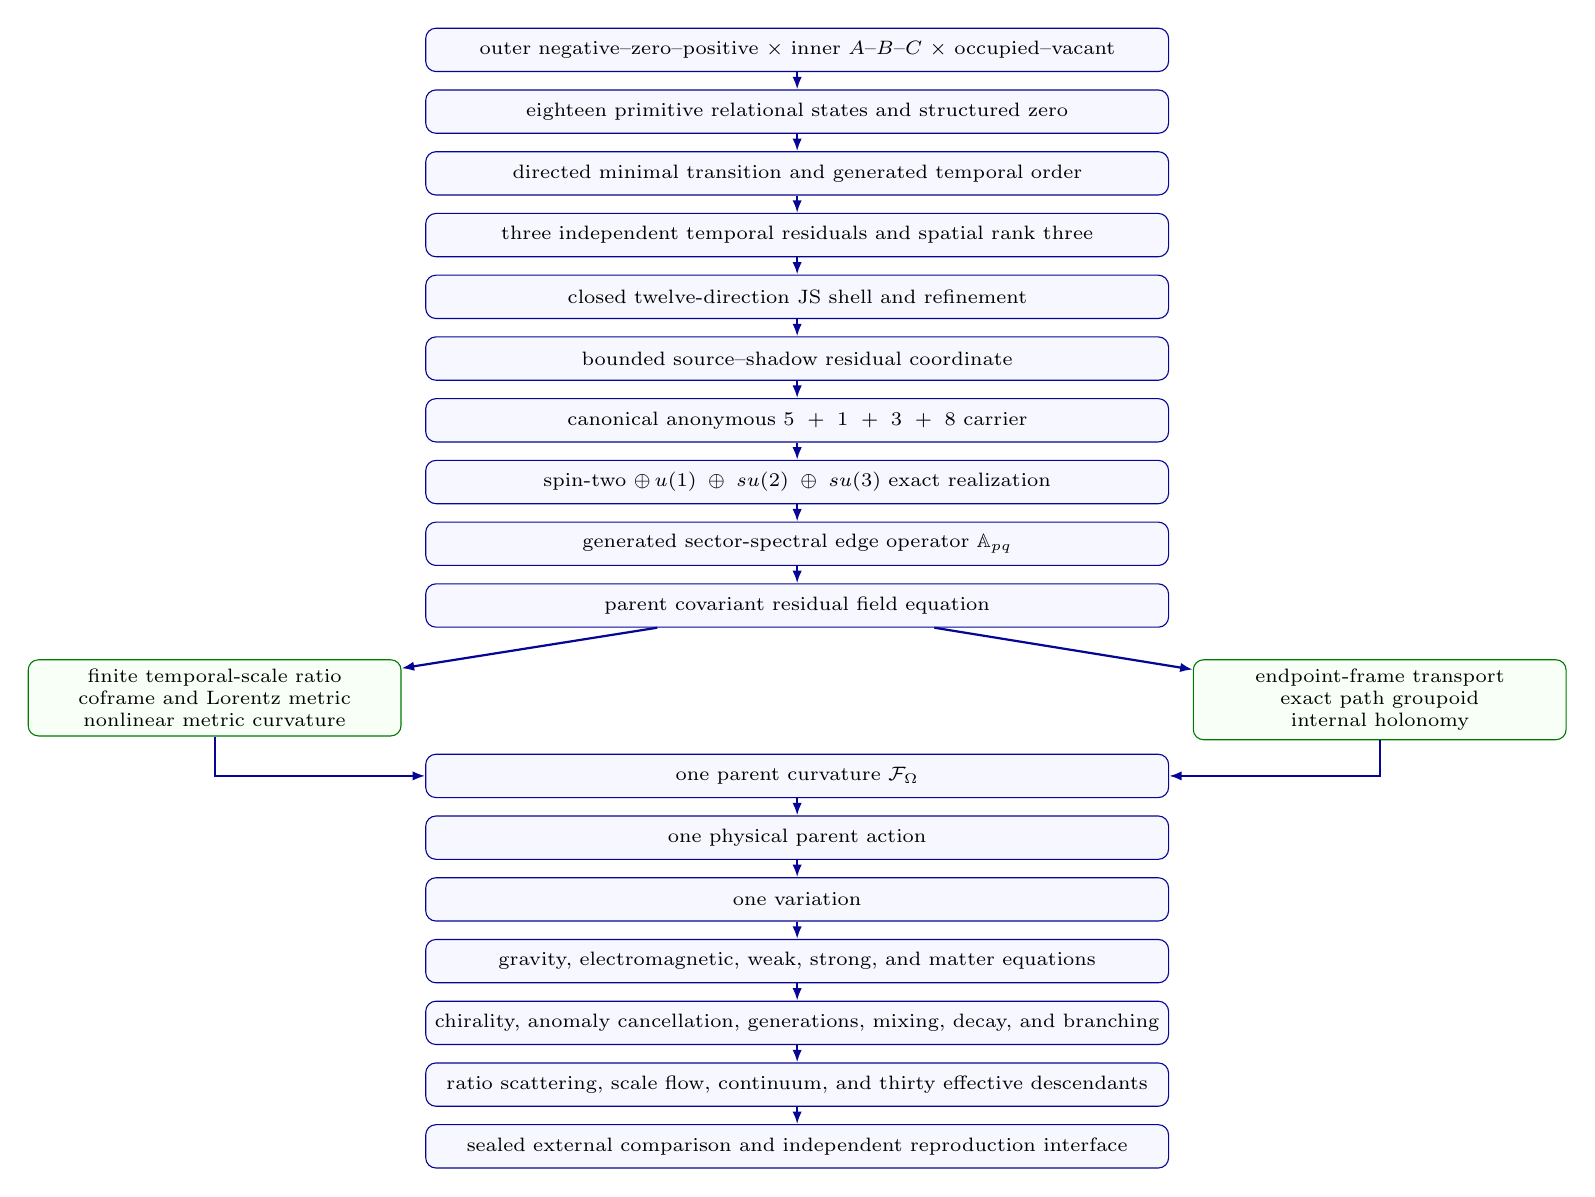
\begin{tikzpicture}[node distance=2.2mm,box/.style={draw=ledgerblue,rounded corners=1.3mm,fill=blue!3,minimum height=5.5mm,text width=9.2cm,align=center,font=\scriptsize},split/.style={draw=ledgergreen,rounded corners=1.3mm,fill=green!3,minimum height=8mm,text width=4.5cm,align=center,font=\scriptsize},arr/.style={-{Latex[length=1.6mm]},thick,draw=ledgerblue}]
\node[box] (a0) {outer negative--zero--positive $\times$ inner $A$--$B$--$C$ $\times$ occupied--vacant};
\node[box,below=of a0] (a1) {eighteen primitive relational states and structured zero};
\node[box,below=of a1] (a2) {directed minimal transition and generated temporal order};
\node[box,below=of a2] (a3) {three independent temporal residuals and spatial rank three};
\node[box,below=of a3] (a4) {closed twelve-direction JS shell and refinement};
\node[box,below=of a4] (a5) {bounded source--shadow residual coordinate};
\node[box,below=of a5] (a6) {canonical anonymous $5+1+3+8$ carrier};
\node[box,below=of a6] (a7) {spin-two $\oplus\,u(1)\oplus su(2)\oplus su(3)$ exact realization};
\node[box,below=of a7] (a8) {generated sector-spectral edge operator $\mathbb A_{pq}$};
\node[box,below=of a8] (a9) {parent covariant residual field equation};
\node[split,below left=4mm and 3mm of a9] (g) {finite temporal-scale ratio\\coframe and Lorentz metric\\nonlinear metric curvature};
\node[split,below right=4mm and 3mm of a9] (i) {endpoint-frame transport\\exact path groupoid\\internal holonomy};
\node[box,below=16mm of a9] (a10) {one parent curvature $\mathcal F_\Omega$};
\node[box,below=of a10] (a11) {one physical parent action};
\node[box,below=of a11] (a12) {one variation};
\node[box,below=of a12] (a13) {gravity, electromagnetic, weak, strong, and matter equations};
\node[box,below=of a13] (a14) {chirality, anomaly cancellation, generations, mixing, decay, and branching};
\node[box,below=of a14] (a15) {ratio scattering, scale flow, continuum, and thirty effective descendants};
\node[box,below=of a15] (a16) {sealed external comparison and independent reproduction interface};
\foreach \u/\v in {a0/a1,a1/a2,a2/a3,a3/a4,a4/a5,a5/a6,a6/a7,a7/a8,a8/a9,a10/a11,a11/a12,a12/a13,a13/a14,a14/a15,a15/a16}{\draw[arr] (\u)--(\v);}
\draw[arr] (a9)--(g); \draw[arr] (a9)--(i); \draw[arr] (g.south) |- (a10.west); \draw[arr] (i.south) |- (a10.east);
\end{tikzpicture}%
}
\caption{Authoritative causal proof map generated from the standalone dependency spine. The central residual equation occurs after the primitive grammar, temporal residual space, JS shell, canonical carrier, exact algebra, and generated edge spectrum. Gravity and internal holonomy are two descendants of the same finite middle law and enter one parent curvature and one physical action.}
\label{fig:causal}
\end{figure}

\clearpage
\begin{figure}[htbp]
\centering
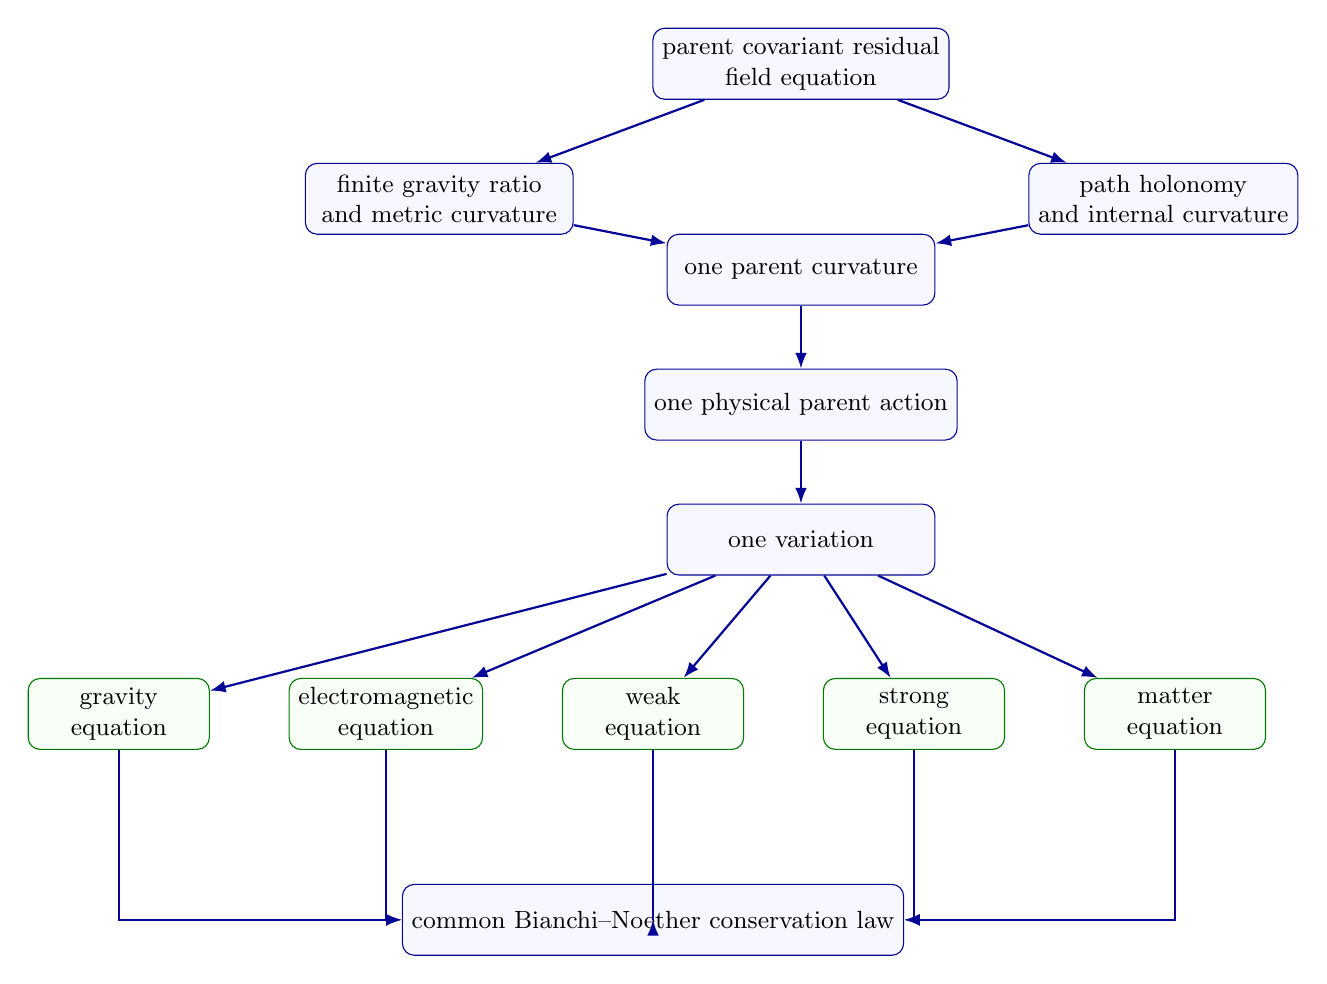
\begin{tikzpicture}[node distance=8mm and 10mm,box/.style={draw=ledgerblue,rounded corners=1.5mm,fill=blue!3,minimum width=3.4cm,minimum height=9mm,align=center,font=\small},force/.style={draw=ledgergreen,rounded corners=1.5mm,fill=green!3,minimum width=2.3cm,minimum height=9mm,align=center,font=\small},arr/.style={-{Latex[length=2mm]},thick,draw=ledgerblue}]
\node[box] (R) {parent covariant residual\\field equation};
\node[box,below left=of R] (G0) {finite gravity ratio\\and metric curvature};
\node[box,below right=of R] (H0) {path holonomy\\and internal curvature};
\node[box,below=17mm of R] (F) {one parent curvature};
\node[box,below=of F] (S) {one physical parent action};
\node[box,below=of S] (V) {one variation};
\node[force,below left=13mm and 58mm of V] (G) {gravity\\equation};
\node[force,right=of G] (E) {electromagnetic\\equation};
\node[force,right=of E] (W) {weak\\equation};
\node[force,right=of W] (C) {strong\\equation};
\node[force,right=of C] (M) {matter\\equation};
\node[box,below=17mm of W] (B) {common Bianchi--Noether conservation law};
\draw[arr] (R)--(G0); \draw[arr] (R)--(H0); \draw[arr] (G0)--(F); \draw[arr] (H0)--(F); \draw[arr] (F)--(S); \draw[arr] (S)--(V);
\foreach \x in {G,E,W,C,M}{\draw[arr] (V)--(\x); \draw[arr] (\x) |- (B);}
\end{tikzpicture}
\caption{Residual-to-variation structure. The nonnegative residual consistency functional is not a second action and does not appear in this physical variation diagram.}
\label{fig:variation}
\end{figure}
\clearpage


\section*{Notation, object types, and input--output rules}
\addcontentsline{toc}{section}{Notation, object types, and input--output rules}

\begin{interpretivebridge}{why a complete symbol dictionary is required}
The central equations are operator equations, not ordinary scalar formulas into which arbitrary measured numbers are inserted. A reader must know the type, dimension, domain, construction rule, and input--output role of every symbol before attempting a calculation. The tables below give that information before the compact equation map is displayed.
\end{interpretivebridge}

\subsection*{General algebraic conventions}
All finite primitive counts and ratio calculations use exact integers or rational numbers. Matrix-valued quantities act on the generated seventeen-dimensional nonconstant carrier unless a smaller projected block is explicitly indicated. The symbols $p$ and $q$ denote the initial and terminal vertices of an oriented generated edge; in a depth-labelled realization, $q-p$ is the integer depth increment. The symbol $I_n$ is the identity on an $n$-dimensional carrier, $X^{-1}$ denotes an inverse on the stated admissible domain, $\oplus$ denotes an orthogonal direct sum, and $\langle\cdot,\cdot\rangle$ denotes the generated invariant inner product or its spacetime-integrated extension.

\begin{longtable}{p{2.1cm}p{3.1cm}p{3.2cm}p{5.6cm}}
\toprule
Symbol & Name & Mathematical type & Meaning, construction, and use\\
\midrule\endhead
$\mathcal A$ & primitive relational alphabet & finite set of size $18$ & The product of outer sign, inner relation, and occupancy. It is generated before time or space and is not a fitted data table.\\
$\Sigma_{\rm out}$ & outer relation set & $\{-1,0,+1\}$ & Negative, balanced, and positive comparison of the selected whole with an exterior reference.\\
$\Sigma_{\rm in}$ & inner relation set & $\{A,B,C\}$ & Inner negative, zero, and positive roles, encoded by $A\mapsto-1$, $B\mapsto0$, $C\mapsto+1$.\\
$\Omega_{\rm occ}$ & occupancy set & $\{0,1\}$ & Vacant and occupied status, independent of the relational sign.\\
$\chi_{\rm out},\chi_{\rm in},\chi_{\rm occ}$ & primitive characters & scalar functions on $\mathcal A$ & Exact numerical readouts of outer orientation, inner orientation, and centered occupancy.\\
$\Delta\chi$ & temporal residual vector & vector in $\Q^3$ & The ordered difference of the three primitive characters across one directed update.\\
$\mathcal H_{18}$ & complete parent function space & $18$-dimensional inner-product space & All real functions on the eighteen primitive states.\\
$\mathcal H_0$ & constant mode & rank-$1$ subspace & The uniform function removed before the nonconstant interaction carrier is formed.\\
$\mathcal H_5$ & metric-response block & rank-$5$ subspace & Symmetric tracefree spatial response, identified with the gravity role only after its operational signature is proved.\\
$\mathcal H_1$ & central internal block & rank-$1$ subspace & One-dimensional anti-Hermitian center, identified with the electromagnetic role.\\
$\mathcal H_3$ & two-state compact block & rank-$3$ subspace & Exact compact three-generator algebra with the weak operational signature.\\
$\mathcal H_8$ & three-state traceless compact block & rank-$8$ subspace & Exact traceless anti-Hermitian $3\times3$ algebra with the strong operational signature.\\
$P_{\rm G},P_{\rm E},P_{\rm W},P_{\rm S}$ & canonical projectors & $17\times17$ idempotent operators & Orthogonal projections onto ranks $5,1,3,8$. They are generated by conditional expectations, not inserted as force labels.\\
$\lambda_i$ & generated sector response ratio & positive rational scalar & The normalized response spectrum $(153,68,108,180)/509$ in the order E, W, S, G. These are internal dimensionless ratios, not measured coupling constants.\\
$X_p$ & source bounded shadow & positive $17\times17$ operator & The state at edge origin $p$, with spectrum strictly inside $(0,1)$. It is an admissible initial condition or a result of an earlier edge update.\\
$\mathcal R(X)$ & exact residual coordinate & matrix function & $\mathcal R(X)=(I-X)X^{-1}$. It maps a bounded shadow bijectively to a positive residual.\\
$R_p,R_q$ & source and target residuals & positive operators & Abbreviations for $\mathcal R(X_p)$ and $\mathcal R(X_q)$. The target is calculated, not inserted.\\
$a_i(p,q)$ & sector edge multiplier & positive rational scalar & The finite response multiplier on sector $i$ across edge $p\to q$.\\
$N(p)$ & local temporal scale & positive scalar & Generated local clock-scale factor at $p$. Only the ratio $N(q)/N(p)$ enters the primitive finite gravity relation.\\
$\mathbb A_{pq}$ & sector-spectral edge operator & positive block-scalar $17\times17$ operator & $\sum_i a_i(p,q)P_i$. It supplies finite compression while preserving the canonical decomposition.\\
$U_{pq}$ & parent frame transport & invertible block-preserving operator & Carries a source frame at $p$ to the target frame at $q$. In exact finite examples it is constructed by rational Cayley transforms.\\
$R_{\rm G}$ & gravitational residual block & operator on $\mathcal H_5$ & The $P_{\rm G}$ projection of the complete residual.\\
$R_{\rm G}^{U}(p)$ & transported source gravity residual & operator on $\mathcal H_5$ & $U_{{\rm G},pq}R_{\rm G}(p)U_{{\rm G},pq}^{-1}$.\\
$\Delta N$ & finite clock-scale increment & scalar & $N(q)-N(p)$. It is used before any differential limit.\\
$H_{\square}$ & plaquette holonomy & invertible matrix & Ordered product of four rational link transports around one elementary closed path.\\
$\epsilon$ & formal expansion parameter & indeterminate & A coefficient-bookkeeping symbol in $\Q[\epsilon]/(\epsilon^3)$, not an experimentally fitted small number.\\
$[Y,X]$ & commutator & matrix & $YX-XY$ under the convention used in the plaquette expansion.\\
$\Omega$ & parent connection & matrix-valued one-form & Local generator of parent frame transport on the generated carrier.\\
$\mathcal F_{\Omega}$ & parent curvature & matrix-valued two-form & $d\Omega+\Omega\wedge\Omega$, obtained from link variation and noncommuting holonomy.\\
$\mathbb M$ & response metric & positive block-diagonal operator & Weights the curvature sectors in the single parent action and is diagonal on the canonical projectors.\\
$\Psi$ & parent matter field & section of generated matter representation & Contains the chiral matter components after the force carrier has been generated.\\
$\bar\Psi$ & conjugate matter field & dual section & The appropriate adjoint or conjugate variable varied independently in the matter Euler--Lagrange equation.\\
$\mathcal D_{\Omega}$ & covariant matter operator & first-order differential operator & The generated matter operator coupled to the parent connection.\\
$V_{\rm rad}(\Psi)$ & radial matter potential & gauge-invariant scalar functional & The generated radial/self-interaction contribution in the matter sector.\\
$S_{\rm parent}$ & physical parent action & scalar functional & The sole physical variational object. Its connection variation yields the four projected field equations; its matter variation yields the matter equation.\\
$C_{\rm res}$ & residual consistency functional & nonnegative scalar & A certificate that the finite middle equation holds on every edge. It is not varied and does not define a fifth force.\\
\bottomrule
\end{longtable}

\subsection*{Which quantities are supplied, generated, and returned?}
For one edge update, the independent supplied data are an admissible source state $X_p$, an oriented edge $p\to q$, and the generated frame/link data appropriate to that edge. The projectors, response ratios, and block structure are fixed by earlier theorems. The edge operator $\mathbb A_{pq}$ and transport $U_{pq}$ are then constructed. The central equation returns one and only one target residual $R_q$ and one and only one target shadow $X_q$.

\begin{center}
\begin{tabular}{p{3.2cm}p{10.8cm}}
\toprule
Role & Objects\\
\midrule
Supplied at the edge & $p,q$, an admissible $X_p$, and the generated local link/frame data\\
Already fixed by earlier proofs & $P_i$, $\lambda_i$, the carrier dimensions, the inner products, and the admissible domains\\
Constructed for the edge & $a_i(p,q)$, $\mathbb A_{pq}$, $U_{pq}$, and $R_p=\mathcal R(X_p)$\\
Returned by the equation & $R_q$ and $X_q=(I+R_q)^{-1}$\\
Not inserted & measured coupling constants, measured particle masses, or a desired target value $X_q$\\
\bottomrule
\end{tabular}
\end{center}

\subsection*{Worked scalar reduction}
The matrix equation contains a simple one-sector example. Set $p=0$, $q=1$, choose the electromagnetic block, take $U_{pq}=1$, and choose $X_p=1/2$. Then
\begin{align}
R_p&=\frac{1-X_p}{X_p}=1,\\
a_{\rm E}(0,1)&=\lambda_{\rm E}=\frac{153}{509},\\
R_q&=a_{\rm E}(0,1)R_p=\frac{153}{509},\\
X_q&=\frac{1}{1+R_q}=\frac{509}{662}.
\end{align}
The input is the source state and the selected generated edge. The target $X_q$ is the output; it is not chosen in advance.

\subsection*{Worked four-block diagonal reduction}
Let the source residual be block diagonal,
\begin{equation}
R_p=r_{\rm G}P_{\rm G}+r_{\rm E}P_{\rm E}+r_{\rm W}P_{\rm W}+r_{\rm S}P_{\rm S},
\end{equation}
and let $U_{pq}=I$. Orthogonality gives
\begin{equation}
R_q=a_{\rm G}r_{\rm G}P_{\rm G}+a_{\rm E}r_{\rm E}P_{\rm E}+a_{\rm W}r_{\rm W}P_{\rm W}+a_{\rm S}r_{\rm S}P_{\rm S}.
\end{equation}
Thus the four components are not four independently postulated equations; they are the four canonical projections of one parent update.

\clearpage

\section*{Central equations of the theory}
\addcontentsline{toc}{section}{Central equations of the theory}

\begin{interpretivebridge}{how to read the compact equation map}
The displayed equations are a map of the full proof, not a substitute for the definitions and derivations that follow. Every symbol has been typed in the preceding notation section. Each equation group is written in ordinary article format; the box above supplies interpretation only.
\end{interpretivebridge}

\subsection*{I. Primitive grammar, temporal residuals, and generated space}
\begin{align}
\mathcal A&=\{-1,0,+1\}_{\rm out}\times\{A,B,C\}_{\rm in}\times\{0,1\}_{\rm occ},\\
|\mathcal A|&=18,\\
\Delta\chi&=(\Delta\chi_{\rm out},\Delta\chi_{\rm in},\Delta\chi_{\rm occ})^{\mathsf T},\\
\rank\operatorname{span}\{\Delta\chi\}&=3.
\end{align}

\subsection*{II. Projective residual coordinate and nonlinear metric gravity}
\begin{align}
T_a(x)&=\frac{x}{a+(1-a)x},\\
\mathcal R(x)&=\frac{1-x}{x},\\
\mathcal R(T_a(x))&=a\mathcal R(x),\\
e^a&=E^a{}_{\mu}\omega^\mu,\\
g&=\eta_{ab}e^a\otimes e^b,\qquad \eta=\diag(-1,1,1,1).
\end{align}
For $C(u)=1+u+u^2$ and $g_{\mu\nu}=C(u)^2\eta_{\mu\nu}$,
\begin{align}
\operatorname{Scal}(g)&=\frac{12}{C(u)^3},\\
G_{00}&=\frac{3(1+2u)^2}{C(u)^2},\\
G_{ii}&=-\frac{3}{C(u)^2},\\
\nabla_{\mu}G^{\mu}{}_{\nu}&=0.
\end{align}
The notation $C(u)$ is used in this compact map to avoid collision with the primitive alphabet $\mathcal A$ and the edge operator $\mathbb A_{pq}$; later historical formulas may retain $A(u)$ where the context is unambiguous.

\subsection*{III. Canonical parent carrier and generated response spectrum}
\begin{align}
\mathcal H_{18}&=\mathcal H_0\oplus\mathcal H_5\oplus\mathcal H_8\oplus\mathcal H_1\oplus\mathcal H_3,\\
\mathcal H_{17}&=\mathcal H_5\oplus\mathcal H_1\oplus\mathcal H_3\oplus\mathcal H_8,\\
P_{\rm G}+P_{\rm E}+P_{\rm W}+P_{\rm S}&=I_{17},\\
(\lambda_{\rm E},\lambda_{\rm W},\lambda_{\rm S},\lambda_{\rm G})&=\frac1{509}(153,68,108,180).
\end{align}

\subsection*{IV. Parent covariant residual field equation}
\begin{align}
\mathcal R(X)&=(I-X)X^{-1},\qquad X=(I+\mathcal R)^{-1},\\
\mathbb A_{pq}&=\sum_{i\in\{{\rm E,W,S,G}\}}a_i(p,q)P_i,\\
a_i(p,q)&=\lambda_i^{q-p}\quad(i={\rm E,W,S}),\\
a_{\rm G}(p,q)&=\frac{N(q)}{N(p)}\lambda_{\rm G}^{q-p},\\
\mathcal R(X_q)&=\mathbb A_{pq}U_{pq}\mathcal R(X_p)U_{pq}^{-1},\\
X_q&=\left[I+\mathbb A_{pq}U_{pq}(I-X_p)X_p^{-1}U_{pq}^{-1}\right]^{-1}.
\end{align}
The generated edge operator satisfies
\begin{equation}
\mathbb A_{pp}=I,\qquad \mathbb A_{qp}\mathbb A_{pq}=I,\qquad \mathbb A_{qr}\mathbb A_{pq}=\mathbb A_{pr}.
\end{equation}

\subsection*{V. Finite gravity correlation and parent curvature}
After the generated gravity-depth factor is separated,
\begin{align}
N(p)R_{\rm G}(q)&=N(q)U_{{\rm G},pq}R_{\rm G}(p)U_{{\rm G},pq}^{-1},\\
\frac{R_{\rm G}(q)-R_{\rm G}^{U}(p)}{\Delta N}&=\frac{R_{\rm G}^{U}(p)}{N(p)},\\
H_{\square}&=I+\epsilon^2[Y,X]\pmod{\epsilon^3},\\
\mathcal F_{\Omega}&=d\Omega+\Omega\wedge\Omega.
\end{align}

\subsection*{VI. One parent action and one variation}
\begin{align}
S_{\rm parent}[\Omega,\Psi]
&=\frac12\langle\mathcal F_{\Omega},\mathbb M\mathcal F_{\Omega}\rangle
+\langle\bar\Psi,\mathcal D_{\Omega}\Psi\rangle+V_{\rm rad}(\Psi),\\
\delta S_{\rm parent}&=0,\\
P_i\frac{\delta S_{\rm parent}}{\delta\Omega}&=0\quad(i={\rm G,E,W,S}),\\
\frac{\delta S_{\rm parent}}{\delta\bar\Psi}&=0.
\end{align}

\subsection*{VII. Parent-derived matter-channel dynamics}
For each chiral role $r$,
\begin{align}
T_r&=V_r\Pi_r^{\downarrow},\\
T_r^3&=0,\\
\mathcal A_r&=I+T_r+T_r^2=(I-T_r)^{-1},\\
N_{r,i\to f}&=\mathcal A_r(f,i)\Delta_{if}m_r,\\
B_{r,i\to f}&=\frac{N_{r,i\to f}}{\sum_{k<i}N_{r,i\to k}},\qquad
\sum_{f<i}B_{r,i\to f}=1.
\end{align}

\clearpage
\section{Purpose, proof order, and generated domain}
\begin{interpretivebridge}{the paper is read from cause to consequence}
The proof follows the causal dependency map in \Cref{fig:causal}. Each stage receives objects generated by the preceding stages. The pre-temporal order is logical and establishes the minimal relational distinctions; the directed predecessor--successor relation then establishes temporal and dynamical order. Every section proves one downward arrow in the master map.
\end{interpretivebridge}

The objective is to place the entire argument in one causal dependency chain. Before a temporal order has been generated, the word ``before'' is logical rather than chronological. After the directed transition relation is established, the order becomes temporal and dynamical. \Cref{fig:causal} therefore contains two kinds of arrows but only one proof order: every object on a lower level is defined from objects already established on higher levels.

\begin{definition}[Admissible source class]
An admissible source object is a compatible finite-depth family of functions on words in the primitive alphabet $\mathcal A$, equipped with the generated transition, residual, projection, gauge, and parent-action structures, whose projective energy is finite at every stage and Cauchy in the declared refinement norm.
\end{definition}

\begin{definition}[Complete internal proof]
A theorem is complete on the generated domain when every object in its statement is generated inside the source class, every dependency precedes its use, every displayed ratio is recalculated from primitive data, and the final assertion is invariant under the one remaining common unit orbit.
\end{definition}

\begin{remark}[Internal and external conclusions]
Internal closure means that the declared parent grammar, its shadow projectors, field equations, and exact certificates are generated without runtime use of an external measurement. It does not convert an internal Boolean result into empirical confirmation. Historical formula provenance, identification with measured observables, and third-party reproduction are evaluated outside the internal theorem gate.
\end{remark}

\begin{proofguide}{Temporal-residual parent--shadow four-interaction theorem}
The following formal result closes the next dependency step. The box states only the reader-facing role; the complete mathematical statement, displayed calculations, and proof remain in the ordinary unboxed format below.
\end{proofguide}
\begin{theorem}[Temporal-residual parent--shadow four-interaction theorem]
Within the admissible source class, the following statements hold in dependency order.
\begin{enumerate}
\item The irreducible outer-sign, inner-relation, occupancy grammar has $18$ primitive states.
\item A directed minimal transition generates one temporal order.
\item Three independent temporal residual characters generate spatial rank three.
\item Their closure generates the JS shell and a $1+3$ causal coframe.
\item Uniform conditional expectations of the three primitive factors generate the canonical projector ranks $1+5+8+1+3=18$, hence the anonymous nonconstant shadow ranks $5+1+3+8=17$.
\item Every admissible simultaneous relation relabeling and occupancy complement preserves these projectors; all four anonymous shadows occur together and no competing path selection is required.
\item The actual JS convolution has exact quadratic isotropy and fourth-order directional spread $2/(9N)$, which tends to zero in the declared refinement limit.
\item The bounded source--shadow map has an exact rational residual coordinate in which projective compression is multiplication and an additive logarithmic coordinate is optional rather than native.
\item One parent covariant residual field equation transports all four canonical sectors, is gauge covariant, composes on paths, and generates finite holonomy.
\item Common-scale invariance and path composition uniquely fix the gravitational edge factor to $N(q)/N(p)$, yielding a finite logarithm-free gravity correlation and the connection coefficient $dN/N$.
\item In the generated second-residual local class, unit normalization uniquely fixes $A(u)=1+u+u^2$.
\item Spatially nonuniform temporal compression produces the universal metric response identified as gravity.
\item The $5$, $1$, $3$, and $8$ modules have the operational signatures of gravity, electromagnetism, weak interaction, and strong interaction, respectively.
\item The loop defect of the covariant residual equation generates the common parent curvature, and one parent action and one variation generate all four field equations and the matter equation.
\item A typed formula grammar fixes the bilinear response and unit-sum normalization without target values and seals the prospective packet before external comparison.
\item The admissible source and shadow continuum descriptions are bilaterally equivalent modulo generated gauge and coordinate equivalence.
\item One time anchor fixes the sole global unit orbit and thereby fixes every dimensionful decoder.
\item The thirty principal effective-equation forms descend through proved native mechanisms and commuting trajectory diagrams.
\item All $525$ executable theorem roots and all $544$ explicit derivations are recorded in the complete proof compendium.
\end{enumerate}
\end{theorem}

\begin{proof}
The primitive grammar, temporal residual, dimensional genesis, JS geometry, canonical parent--shadow decomposition, source--shadow depth, coframe, carrier decomposition, covariant residual field equation, finite gravity correlation, curvature descent, nonlinear gravity, internal interaction, matter, parent action, continuum, unit-decoder, and prediction sections prove the statements in the displayed order. The complete conjunction is restated in \Cref{sec:conclusion}, and every executable root is indexed in the accompanying Supplementary Proof Record.
\end{proof}



\begin{proofguide}{Authoritative causal spine completion}
The full manuscript and the executable use one dependency order only. This theorem rules out obsolete proof maps and fixes the location of the parent covariant residual field equation between the generated carrier and the common curvature-action system.
\end{proofguide}
\begin{proofguide}{Authoritative causal spine completion}
The following formal result closes the next dependency step. The box states only the reader-facing role; the complete mathematical statement, displayed calculations, and proof remain in the ordinary unboxed format below.
\end{proofguide}
\begin{theorem}[Authoritative causal spine completion]
The complete construction has the unique declared order: relational grammar, directed time, three temporal residuals, spatial rank three, JS shell, bounded residual coordinate, canonical $5+1+3+8$ carrier, exact operational algebras, generated edge spectrum, parent covariant residual field equation, finite gravity correlation and internal holonomy, parent curvature, one physical parent action, matter, ratio observables, continuum descendants, and an external comparison interface.
\end{theorem}
\begin{proof}
Every object in the list is required by the next object and is generated before its first use. The directed transition is required to define temporal residuals; the residual span is required to define the spatial and shell carriers; the canonical projectors are required to define the sector-spectral edge operator; the finite residual equation is required to define both the gravitational clock comparison and the closed-path holonomy; those two mechanisms generate the parent curvature used by the sole physical action. Matter and observables are defined only after the carrier, connection, and action. The dependency graph is acyclic, and any reordering that places a descendant before one of these antecedents leaves an undefined symbol. Hence the declared spine is authoritative on the generated class.
\end{proof}
\section{Pre-temporal relational grammar}
\begin{conceptledger}{why the proof starts with relations rather than objects}
The primitive stage consists solely of comparative relations. Relative to a selected reference, a relation has negative orientation, relational balance, or positive orientation; the same distinction occurs inside the selected sector; and each inner seat is occupied or vacant. These three independent questions generate the minimal relational ledger used by every later construction.
\end{conceptledger}

\label{sec:grammar}

\subsection{Outer relation, inner relation, and occupancy}
\begin{interpretivebridge}{negative, zero, and positive are directions of comparison}
Negative and positive denote opposite orientations of a relation with respect to a reference: deficit versus surplus, inward versus outward, or opposed versus aligned. Reversing the reference reverses their signs. Zero is the fixed relational position at which the selected signed difference vanishes.
\end{interpretivebridge}
\begin{conceptledger}{complementary zero readouts across occupancy and residual contrast}
Zero has several readouts. It is \emph{empty zero} when the occupancy count equals zero; \emph{balanced zero} when opposed occupied contributions cancel; \emph{saturated-relative zero} when a selected sector is completely filled and its remaining internal contrast equals zero; and \emph{rebased zero} when a completed whole becomes the origin of a deeper comparison. A closed state therefore reads as zero under residual contrast while reading as complete under occupancy of its own domain. The two readouts are complementary.
\end{conceptledger}
\begin{interpretivebridge}{why every outer sign contains the same six inner states}
The outer sign tells how the whole selected sector compares with its exterior. The inner label tells how a relation inside that sector is directed. Occupancy tells whether that inner relation is full or vacant. Because these questions are independent, each outer negative, zero, or positive sector contains an inner negative, zero, and positive seat, and each inner seat may be occupied or vacant. This is the origin of the six inner states inside each of the three outer states and hence of the eighteen-state grammar.
\end{interpretivebridge}

Let
\begin{equation}
\Sigma_{\rm out}=\{-1,0,+1\},\qquad
\Sigma_{\rm in}=\{A,B,C\},\qquad
\Omega=\{0,1\}.
\end{equation}
The inner labels are ordered relational roles,
\begin{equation}
A\leftrightarrow -1,\qquad B\leftrightarrow 0,\qquad C\leftrightarrow +1,
\end{equation}
while the occupancy label is $0$ for vacant and $1$ for occupied. A primitive state is
\begin{equation}
\alpha=(s,r,o)\in\mathcal A:=\Sigma_{\rm out}\times\Sigma_{\rm in}\times\Omega.
\end{equation}
Thus every outer negative, outer zero, and outer positive state contains an inner negative, inner zero, and inner positive relation, each either occupied or vacant.

\begin{center}
\small
\begin{tabular}{c|cc|cc|cc}
\toprule
Outer state & occupied $A$ & vacant $A$ & occupied $B$ & vacant $B$ & occupied $C$ & vacant $C$\\
\midrule
$-1$ & $(-1,A,1)$ & $(-1,A,0)$ & $(-1,B,1)$ & $(-1,B,0)$ & $(-1,C,1)$ & $(-1,C,0)$\\
$0$ & $(0,A,1)$ & $(0,A,0)$ & $(0,B,1)$ & $(0,B,0)$ & $(0,C,1)$ & $(0,C,0)$\\
$+1$ & $(+1,A,1)$ & $(+1,A,0)$ & $(+1,B,1)$ & $(+1,B,0)$ & $(+1,C,1)$ & $(+1,C,0)$\\
\bottomrule
\end{tabular}
\end{center}

\begin{axiom}[Primitive relational completeness]
A primitive grammar must distinguish an outer comparison direction, an inner relation direction, and occupied/vacant complementarity. Each distinction must contain a reversible sign pair and a relational zero.
\end{axiom}

\begin{proofguide}{State count}
The following formal result closes the next dependency step. The box states only the reader-facing role; the complete mathematical statement, displayed calculations, and proof remain in the ordinary unboxed format below.
\end{proofguide}
\begin{lemma}[State count]
The primitive grammar contains exactly $18$ states.
\end{lemma}
\begin{proof}
The three factors are independent at the primitive level, hence
\begin{equation}
|\mathcal A|=|\Sigma_{\rm out}|\,|\Sigma_{\rm in}|\,|\Omega|=3\cdot3\cdot2=18.
\end{equation}
Componentwise equality in the Cartesian product makes all eighteen listed states distinct.
\end{proof}

\begin{proofguide}{Minimality of the $3\times3\times2$ grammar}
The following formal result closes the next dependency step. The box states only the reader-facing role; the complete mathematical statement, displayed calculations, and proof remain in the ordinary unboxed format below.
\end{proofguide}
\begin{theorem}[Minimality of the $3\times3\times2$ grammar]
Among finite Cartesian grammars satisfying primitive relational completeness, the minimum cardinality that preserves all three requirements is eighteen.
\end{theorem}
\begin{proof}
A reversible comparison layer requires at least two nonzero directions and one fixed relational zero, so each sign layer has cardinality at least three. Occupancy complementarity requires at least two states. Therefore every admissible product grammar has at least $3\cdot3\cdot2=18$ states. The displayed alphabet attains this bound.
\end{proof}


\begin{proofguide}{Complete eighteen-state semantic bijection}
This result translates the abstract Cartesian product into the full occupied/vacant semantic ledger and confirms that no primitive state is duplicated or omitted.
\end{proofguide}
\begin{theorem}[Complete eighteen-state semantic bijection]
The eighteen tuples are in one-to-one correspondence with the occupied and vacant inner negative, zero, and positive relations inside each outer negative, zero, and positive sector.
\end{theorem}
\begin{proof}
Map $(s,A,o)$ to the inner-negative state of occupancy $o$ inside outer sector $s$, map $(s,B,o)$ to the inner-zero state, and map $(s,C,o)$ to the inner-positive state. The outer sign, inner role, and occupancy are recovered uniquely from the semantic description, so the map is injective and surjective. The table therefore contains exactly six states in each outer sector and eighteen in total.
\end{proof}

\subsection{Structured zero and global minimality}
\begin{conceptledger}{zero combines relational position with an independent occupancy value}
Each outer negative, zero, and positive relation contains the same six inner states: occupied or vacant inner negative, zero, and positive. Occupancy and relational position are independent. Consequently an empty zero and a full zero are distinct states, while a completely saturated layer has zero internal contrast and becomes the centered reference of the next recursive layer.
\end{conceptledger}
\begin{proofguide}{Structured-zero recursive semantics}
The following formal result closes the next dependency step. The box states only the reader-facing role; the complete mathematical statement, displayed calculations, and proof remain in the ordinary unboxed format below.
\end{proofguide}
\begin{theorem}[Structured-zero recursive semantics]
The primitive product contains exactly eighteen distinct states, six in each outer relation. Empty zero and full zero both exist, and centering any uniformly saturated negative, zero, or positive layer yields the zero vector of the next relational level.
\end{theorem}
\begin{proof}
The Cartesian product gives the eighteen rows explicitly. Fixing an outer sign leaves three inner signs times two occupancy states, hence six rows. The rows $(0,B,0)$ and $(0,B,1)$ witness empty and full zero. For a saturated layer $(s,s,s)$ its mean is $s$, so subtraction of the mean gives $(0,0,0)$ for $s=-1,0,+1$.
\end{proof}
\begin{proofguide}{Global minimum in the declared finite relational category}
The following formal result closes the next dependency step. The box states only the reader-facing role; the complete mathematical statement, displayed calculations, and proof remain in the ordinary unboxed format below.
\end{proofguide}
\begin{theorem}[Global minimum in the declared finite relational category]
Among finite product grammars with a reversible sign pair and distinguished zero in each of the two sign layers, together with one empty--full complement, the unique irreducible minimum is $(3,3,2)$ and contains eighteen states.
\end{theorem}
\begin{proof}
Each reversible sign layer has odd cardinality at least three. The occupancy complement has even cardinality at least two. The product is therefore at least eighteen. Equality forces $(3,3,2)$. Any larger admissible factor contributes an additional independent reversal pair or complement pair and is reducible relative to the declared primitive requirements.
\end{proof}

\subsection{Primitive characters}
\begin{interpretivebridge}{characters convert qualitative relations into exact residual coordinates}
The three characters are numerical readouts of outer orientation, inner orientation, and occupancy complement. Their ordered differences generate the independent residual directions of space.
\end{interpretivebridge}

Define the three centered characters
\begin{align}
\chi_{\rm out}(s,r,o)&=s,\\
\chi_{\rm in}(s,r,o)&=\iota(r),\qquad \iota(A)=-1,\ \iota(B)=0,\ \iota(C)=+1,\\
\chi_{\rm occ}(s,r,o)&=2o-1.
\end{align}
The outer and inner characters carry relational orientation, and the occupancy character carries the occupied/vacant complement. Spatial coordinates and force labels are generated at later stages.

\section{Temporal order and residual genesis}
\begin{conceptledger}{time is generated first and three spatial directions follow: the order is $1+3$}
The usual notation ``three space dimensions plus time'' describes an already formed spacetime. The present proof has a different causal order. A directed succession of relational states first generates one temporal order. Only changes along that order produce three independent residual records, and those residuals then require a three-dimensional spatial carrier. The generated dependency is therefore one temporal order followed by three spatial directions: $1+3$.
\end{conceptledger}

\label{sec:time}

\subsection{Directed minimal transitions}
\begin{interpretivebridge}{directed transition converts relational states into temporal order}
The eighteen states by themselves are static possibilities. Time appears only when an actual transition selects a predecessor and a successor. Counting successive directed updates provides the minimal clock. Any other clock that advances uniformly along the same history differs only by an origin and a positive scale.
\end{interpretivebridge}

\begin{definition}[Minimal transition]
Two primitive states are minimally adjacent when they differ in exactly one primitive coordinate by one admissible step: $-1\leftrightarrow0\leftrightarrow+1$ in a sign layer or $0\leftrightarrow1$ in occupancy.
\end{definition}

\begin{axiom}[Directed update]
An actual update selects one orientation of a minimal adjacency as predecessor and successor. The resulting update graph is acyclic on every finite history.
\end{axiom}

\begin{definition}[Generated time]
For a finite directed history
\(
\alpha_0\to\alpha_1\to\cdots\to\alpha_n
\),
the temporal coordinate is its order rank $t(\alpha_k)=k$.
\end{definition}

\begin{proofguide}{Time-origin uniqueness}
The following formal result closes the next dependency step. The box states only the reader-facing role; the complete mathematical statement, displayed calculations, and proof remain in the ordinary unboxed format below.
\end{proofguide}
\begin{theorem}[Time-origin uniqueness]
On a connected directed history, every scalar coordinate that strictly increases by one on every primitive update differs from $t$ by an additive constant. If an arbitrary positive step size is admitted, it differs by a positive affine transformation.
\end{theorem}
\begin{proof}
Let $\tau$ be another coordinate with $\tau(\alpha_{k+1})-\tau(\alpha_k)=1$. Telescoping gives $\tau(\alpha_k)=\tau(\alpha_0)+k=t(\alpha_k)+\tau(\alpha_0)$. With constant positive increment $c$, the same argument gives $\tau=ct+b$.
\end{proof}

\begin{remark}
Time is the ordered succession of actual relational updates; the static alphabet supplies the states on which that order acts.
\end{remark}

\subsection{Temporal residual vector}
\begin{interpretivebridge}{a residual is what an update fails to erase}
An update can alter the outer relation, the inner relation, or occupancy. The difference between successive character values records what remains after the update. Because the three primitive distinctions can change independently, their residuals are independent surviving relational degrees of freedom from which the next structural layer is built.
\end{interpretivebridge}

For a directed transition $\alpha_k\to\alpha_{k+1}$ define
\begin{equation}
\Delta\chi_k=
\begin{pmatrix}
\chi_{\rm out}(\alpha_{k+1})-\chi_{\rm out}(\alpha_k)\\
\chi_{\rm in}(\alpha_{k+1})-\chi_{\rm in}(\alpha_k)\\
\frac12\bigl(\chi_{\rm occ}(\alpha_{k+1})-\chi_{\rm occ}(\alpha_k)\bigr)
\end{pmatrix}
\in\Q^3.
\end{equation}
The components are called the outer-sign residual, inner-relation residual, and occupancy residual.

\begin{proofguide}{Independent residual witnesses}
The following formal result closes the next dependency step. The box states only the reader-facing role; the complete mathematical statement, displayed calculations, and proof remain in the ordinary unboxed format below.
\end{proofguide}
\begin{lemma}[Independent residual witnesses]
The transition set contains three residuals proportional to the standard basis of $\Q^3$.
\end{lemma}
\begin{proof}
Choose transitions that modify only one character:
\begin{align}
(-1,B,0)&\to(0,B,0),&\Delta\chi&=(1,0,0),\\
(0,A,0)&\to(0,B,0),&\Delta\chi&=(0,1,0),\\
(0,B,0)&\to(0,B,1),&\Delta\chi&=(0,0,1).
\end{align}
\end{proof}

\begin{proofguide}{Temporal residual rank}
The following formal result closes the next dependency step. The box states only the reader-facing role; the complete mathematical statement, displayed calculations, and proof remain in the ordinary unboxed format below.
\end{proofguide}
\begin{theorem}[Temporal residual rank]
The temporal residual space has rank three.
\end{theorem}
\begin{proof}
Every residual has three components, hence the rank is at most three. The three witnesses in the preceding lemma are linearly independent, hence the rank is at least three.
\end{proof}

\begin{interpretivebridge}{time to space}
The three residual components are independent records of one ordered update. Their simultaneous independence defines the generated spatial carrier.
\end{interpretivebridge}

\section{Residual dimensional genesis and JS shell geometry}
\begin{conceptledger}{dimension is the number of independent residual directions that must coexist}
The three linearly independent temporal residual characters have minimal injective carrier rank three. Their residual independence therefore generates three-dimensional space after temporal order.
\end{conceptledger}

\label{sec:space}

\subsection{Spatial carrier}
\begin{interpretivebridge}{from one ordered axis to three residual axes}
The temporal axis orders events, while the three residual components coordinate differences produced along that order. Their span is the minimal spatial carrier. This establishes the causal ordering $1\rightarrow3$.
\end{interpretivebridge}

\begin{definition}[Generated spatial carrier]
The spatial carrier is the residual span
\begin{equation}
V_{\rm space}:=\operatorname{span}_{\Q}\{\Delta\chi_k\}\cong\Q^3.
\end{equation}
\end{definition}

\begin{proofguide}{Dimension-genesis theorem}
The following formal result closes the next dependency step. The box states only the reader-facing role; the complete mathematical statement, displayed calculations, and proof remain in the ordinary unboxed format below.
\end{proofguide}
\begin{theorem}[Dimension-genesis theorem]
The minimal injective spatial rank for all temporal residuals is three.
\end{theorem}
\begin{proof}
Injective representation of the residual span requires a target dimension at least its rank, which is three. The identity representation in $\Q^3$ attains the bound.
\end{proof}


\begin{proofguide}{Time-residual-dimension strict dependency}
The theorem below prevents the causal narrative from being read backwards. Space is not assumed before time; spatial rank is the rank of residual records generated by directed temporal updates.
\end{proofguide}
\begin{theorem}[Time-residual-dimension strict dependency]
Directed update generates temporal order first; the three independent character differences are generated second; their rank-three span is generated third; and the closed JS shell is generated fourth.
\end{theorem}
\begin{proof}
Without an oriented update there is no predecessor--successor difference and therefore no $\Delta\chi$. Once the update is oriented, the three character differences are defined. The three explicit witness transitions in the outer, inner, and occupancy factors are linearly independent, while $\Delta\chi$ has only three components, so its span has rank exactly three. The JS directions are signed two-axis combinations of these three generated residual axes and therefore cannot be defined before the residual span. This proves the strict dependency.
\end{proof}

\subsection{Unique causal signature under isotropic residual symmetry}
\begin{interpretivebridge}{why the temporal sign differs from the three spatial signs}
The three residual coordinates are mutually interchangeable under spatial permutation symmetry, whereas the temporal order has a distinguished orientation from predecessor to successor. A nondegenerate quadratic form that respects those roles must give the three residual coordinates equal signs and the temporal coordinate the opposite sign. This produces the Lorentzian $1+3$ signature rather than assuming it.
\end{interpretivebridge}

Let $u^0$ denote temporal order and $u^1,u^2,u^3$ the residual coordinates. The spatial residual labels are permutation symmetric, whereas the temporal coordinate is oriented.

\begin{proofguide}{One-plus-three signature}
The following formal result closes the next dependency step. The box states only the reader-facing role; the complete mathematical statement, displayed calculations, and proof remain in the ordinary unboxed format below.
\end{proofguide}
\begin{theorem}[One-plus-three signature]
Up to a nonzero common factor and overall sign, the unique nondegenerate diagonal quadratic form that preserves spatial permutation symmetry and distinguishes the oriented temporal coordinate from all three residual coordinates is
\begin{equation}
\eta=\diag(-1,1,1,1).
\end{equation}
\end{theorem}
\begin{proof}
Spatial permutation symmetry forces equal spatial diagonal entries. Distinction between temporal and spatial roles forces the temporal coefficient to have the opposite sign. Nondegeneracy excludes zero coefficients. A common factor and overall sign are physically redundant.
\end{proof}

\subsection{Twelve-direction JS shell}
\begin{conceptledger}{why twelve directions form the first closed local shell}
Algebraically, the twelve directions are the signed permutations of $(1,1,0)$: every direction uses two of the three residual axes, is closed under inversion and coordinate permutation, has zero first moment, and has isotropic second moment. Geometrically, the same directions are the centers of twelve congruent spheres touching one congruent central sphere in the three-dimensional kissing configuration. Thus a central spherical shell admits twelve equal touching neighbors, producing a maximally contacted and densely constrained local carrier. The equal-sphere picture geometrically represents the exact twelve-direction incidence and isotropy.
\end{conceptledger}

Define
\begin{equation}
\mathcal V_{12}=\{(\pm1,\pm1,0),(\pm1,0,\pm1),(0,\pm1,\pm1)\}.
\end{equation}
These are the twelve signed two-axis residual directions.

\begin{proofguide}{Isotropy}
The following formal result closes the next dependency step. The box states only the reader-facing role; the complete mathematical statement, displayed calculations, and proof remain in the ordinary unboxed format below.
\end{proofguide}
\begin{lemma}[Isotropy]
The first moment of $\mathcal V_{12}$ vanishes and its normalized second moment is the identity:
\begin{equation}
\sum_{v\in\mathcal V_{12}}v=0,
\qquad
\frac18\sum_{v\in\mathcal V_{12}}vv^{\mathsf T}=I_3.
\end{equation}
\end{lemma}
\begin{proof}
Every direction occurs with its negative, so the first moment vanishes. Each coordinate is nonzero in eight directions and each mixed product cancels by sign symmetry, giving diagonal second moment $8I_3$.
\end{proof}

Define edges between vertices at minimal Euclidean separation. The resulting shell is the cuboctahedral JS relation shell.

\begin{proofguide}{JS shell closure}
The following formal result closes the next dependency step. The box states only the reader-facing role; the complete mathematical statement, displayed calculations, and proof remain in the ordinary unboxed format below.
\end{proofguide}
\begin{theorem}[JS shell closure]
The shell has $12$ vertices, $24$ edges, $8$ triangular faces, and $6$ square faces. Every edge belongs to one triangle and one square, and
\begin{equation}
\chi=12-24+(8+6)=2.
\end{equation}
Hence the shell is a closed sphere-type two-complex.
\end{theorem}

\begin{proof}
Direct enumeration of minimal-distance pairs gives degree four at every vertex and therefore $12\cdot4/2=24$ edges. The signed-coordinate cycles divide into eight triangular and six square faces. The edge-face incidence count is $8\cdot3+6\cdot4=48=2\cdot24$, so every edge is shared by exactly two faces. The Euler count follows.
\end{proof}

\begin{remark}
The generated relation complex supplies a closed local carrier, incidence operators, and isotropic refinement directions.
\end{remark}


\subsection{Refined convolution and directional-isotropy limit}
\begin{interpretivebridge}{the finite shell is refined by its actual path distribution}
Refinement does not assign an external damping coefficient to a precomputed defect. It composes the twelve primitive relation steps, reconstructs the exact $N$-step distribution, and then recomputes its directional moments. The resulting quadratic symbol is isotropic at every level, while the first nontrivial directional defect decreases with the actual number of composed paths.
\end{interpretivebridge}

Let $X$ be uniformly distributed on $\mathcal V_{12}$ and let
\begin{equation}
S_N=X_1+\cdots+X_N
\end{equation}
for independent copies $X_k$. Exact summation gives
\begin{equation}
\mathbb E[X]=0,
\qquad
\mathbb E[XX^{\mathsf T}]=\frac23 I_3,
\qquad
\frac1N\mathbb E[S_NS_N^{\mathsf T}]=\frac23 I_3.
\label{eq:js-covariance}
\end{equation}
For a nonzero probe direction $n$, define the normalized fourth moment
\begin{equation}
M_4(N,n)=\frac{\mathbb E[(n\cdot S_N)^4]}{N^2\|n\|^4}.
\end{equation}
Independence gives
\begin{equation}
M_4(N,n)=\frac43+\frac{\kappa_4(n)}{N\|n\|^4},
\label{eq:fourth-cumulant-law}
\end{equation}
where $\kappa_4(n)$ is the primitive directional fourth cumulant.

\begin{proofguide}{Refined shadow dispersion isotropy}
The following formal result closes the next dependency step. The box states only the reader-facing role; the complete mathematical statement, displayed calculations, and proof remain in the ordinary unboxed format below.
\end{proofguide}
\begin{theorem}[Refined shadow dispersion isotropy]
For axis, face-diagonal, and body-diagonal probes, the exact directional spread is
\begin{equation}
\Delta_4(N)
=\max_n M_4(N,n)-\min_n M_4(N,n)
=\frac{2}{9N}.
\label{eq:anisotropy-spread}
\end{equation}
If refinement level $\ell$ has path count $N=3^\ell$, then
\begin{equation}
\Delta_4(\ell)=\frac{2}{9\cdot3^\ell}\longrightarrow0.
\end{equation}
Every normalized even cumulant of order $2m\ge4$ scales as $N^{1-m}$ and therefore vanishes in the same limit.
\end{theorem}

\begin{proof}
The $N$-step distribution is the exact convolution of the primitive uniform distribution. The fourth moment of an independent sum is
\begin{equation}
\mathbb E[(n\cdot S_N)^4]
=N\mathbb E[(n\cdot X)^4]+3N(N-1)\mathbb E[(n\cdot X)^2]^2.
\end{equation}
Division by $N^2\|n\|^4$ gives \eqref{eq:fourth-cumulant-law}. Exact evaluation on the three inequivalent probe orbits yields the spread \eqref{eq:anisotropy-spread}. Additivity of cumulants gives $\kappa_{2m}(S_N)=N\kappa_{2m}(X)$; normalization by $N^m$ gives $N^{1-m}$. The code verifies the complete convolutions directly for $N=1,2,3,4$ and the general identity by exact induction. The theorem proves the declared refinement limit and does not assert exact continuous Lorentz invariance at a finite level.
\end{proof}

\section{Bounded source--shadow projection}
\begin{conceptledger}{source and shadow are two complete coordinates of one state}
The source variable records an unbounded residual ratio. A finite observer or bounded readout represents the same information by two complementary numbers between zero and one. Their ratio reconstructs the source exactly, so projection changes coordinates and visible shape while preserving the underlying source information.
\end{conceptledger}

\label{sec:shadow}

\subsection{Positive odds and complementary shadow pair}
\begin{interpretivebridge}{why the bounded pair is preferable to a single clipped value}
A single bounded coordinate approaching zero may look singular or information-poor. Its complement approaches one, and the quotient of the pair preserves the complete unbounded odds. The two-boundary representation makes inward and outward readings conjugate parts of one source orbit.
\end{interpretivebridge}

Let $r>0$ be a positive residual odds variable. Define
\begin{equation}
 x=\frac1{1+r},\qquad y=1-x=\frac{r}{1+r},\qquad \frac yx=r.
\end{equation}
The source variable $r$ is unbounded; the shadow pair $(x,y)$ is bounded and preserves complete information because $r=y/x$.

\begin{definition}[Projective boundary compression]
For $a>0$, define
\begin{equation}
T_a(x)=\frac{x}{a+(1-a)x}.
\end{equation}
\end{definition}

\begin{proofguide}{Odds multiplication}
The following formal result closes the next dependency step. The box states only the reader-facing role; the complete mathematical statement, displayed calculations, and proof remain in the ordinary unboxed format below.
\end{proofguide}
\begin{lemma}[Odds multiplication]
\begin{equation}
\frac{1-T_a(x)}{T_a(x)}=a\frac{1-x}{x}.
\end{equation}
\end{lemma}
\begin{proof}
Writing $d=a+(1-a)x$ gives $T_a=x/d$ and $1-T_a=a(1-x)/d$. Their ratio is the stated expression.
\end{proof}

\begin{proofguide}{M\"obius semigroup}
The following formal result closes the next dependency step. The box states only the reader-facing role; the complete mathematical statement, displayed calculations, and proof remain in the ordinary unboxed format below.
\end{proofguide}
\begin{theorem}[M\"obius semigroup]
For positive $a,b$,
\begin{equation}
T_a\circ T_b=T_{ab},\qquad T_1=\Id,\qquad T_a^{-1}=T_{1/a}.
\end{equation}
\end{theorem}
\begin{proof}
The odds map $r=(1-x)/x$ conjugates $T_a$ to multiplication $r\mapsto ar$. Composition, identity, and inversion therefore follow from the multiplicative group of positive rationals or reals.
\end{proof}

\subsection{Invariant depth one-form}
\begin{interpretivebridge}{the depth differential survives every projective readout}
Different positive compression factors alter the bounded coordinate, but the differential ratio $dx/[x(1-x)]$ is unchanged by pullback. This invariant one-form is the local object from which a coordinate-independent depth and, later, a projectively invariant coframe can be constructed.
\end{interpretivebridge}

\begin{proofguide}{Projective depth one-form}
The following formal result closes the next dependency step. The box states only the reader-facing role; the complete mathematical statement, displayed calculations, and proof remain in the ordinary unboxed format below.
\end{proofguide}
\begin{theorem}[Projective depth one-form]
The one-form
\begin{equation}
\omega=\frac{dx}{x(1-x)}
\end{equation}
is invariant under every positive projective compression:
\begin{equation}
T_a^*\omega=\omega.
\end{equation}
\end{theorem}
\begin{proof}
With $d=a+(1-a)x$,
\begin{equation}
T_a'(x)=\frac{a}{d^2},\qquad
T_a(x)(1-T_a(x))=\frac{a x(1-x)}{d^2}.
\end{equation}
Therefore
\begin{equation}
\frac{dT_a(x)}{T_a(x)(1-T_a(x))}
=\frac{a\,dx/d^2}{a x(1-x)/d^2}
=\frac{dx}{x(1-x)}.
\end{equation}
\end{proof}

\begin{remark}
This identity is exact and rational. The computational proof represents the depth structure by exact rational powers and finite additivity. Integration of the invariant one-form or of the multiplicative orbit gives the logarithmic coordinate in the continuum description.
\end{remark}

\section{Additive depth and the multiplicative-to-additive decoder}
\begin{conceptledger}{multiplicative source evolution and its additive logarithmic decoder}
The native temporal process is repeated multiplication of a residual ratio. An observer describes how many primitive compression steps have accumulated by an additive depth. The unique normalized map from multiplication to addition is logarithmic-class. The source computation therefore needs only exact powers and rational transformations; logarithmic notation appears when the multiplicative source orbit is expressed as a continuous additive coordinate.
\end{conceptledger}

\label{sec:depth}

\subsection{Primitive temporal contraction}
\begin{interpretivebridge}{one time step fixes the elementary depth step}
The factor-three source orbit is the reciprocal representation of the primitive temporal contraction selected by the residual grammar. Repetition of the same elementary update produces the full discrete depth hierarchy.
\end{interpretivebridge}

The temporal residual construction selects the reciprocal pair $q=3$ and $c=1/3$. On the source orbit,
\begin{equation}
 r_n=q^n=3^n,
\qquad
 x_n=\frac1{1+3^n}.
\end{equation}
A unit increase of temporal depth multiplies the odds by $3$ and contracts the complementary shadow distance by the corresponding projective step.

\begin{definition}[Normalized additive depth]
A depth decoder on the cyclic orbit $\{q^n:n\in\mathbb Z\}$ is a map $D$ satisfying
\begin{equation}
D(1)=0,
\qquad D(q)=1,
\qquad D(rs)=D(r)+D(s).
\end{equation}
\end{definition}

\begin{proofguide}{Unique depth on the primitive orbit}
The following formal result closes the next dependency step. The box states only the reader-facing role; the complete mathematical statement, displayed calculations, and proof remain in the ordinary unboxed format below.
\end{proofguide}
\begin{theorem}[Unique depth on the primitive orbit]
The unique normalized additive decoder is
\begin{equation}
D(q^n)=n.
\end{equation}
\end{theorem}
\begin{proof}
By additivity, $D(q^n)=nD(q)=n$ for positive $n$. The identity $0=D(1)=D(q^nq^{-n})$ gives $D(q^{-n})=-n$.
\end{proof}

\begin{proofguide}{Continuous logarithmic-class extension}
The following formal result closes the next dependency step. The box states only the reader-facing role; the complete mathematical statement, displayed calculations, and proof remain in the ordinary unboxed format below.
\end{proofguide}
\begin{corollary}[Continuous logarithmic-class extension]
The unique monotone continuous extension to positive real odds is
\begin{equation}
D(r)=\log_q r.
\end{equation}
Equivalently, in the bounded coordinate,
\begin{equation}
D(x)=\log_q\left(\frac{1-x}{x}\right).
\end{equation}
\end{corollary}

\begin{proof}
The continuous homomorphisms from positive multiplication to real addition are constant multiples of the natural logarithm. The normalization $D(q)=1$ fixes the multiple.
\end{proof}

\begin{interpretivebridge}{why a logarithm appears}
The source law is multiplicative residual compression. The observer records the accumulated primitive compression steps by additive depth. The unique inverse coordinate that converts the multiplicative temporal orbit into this additive depth is logarithmic-class.
\end{interpretivebridge}

\subsection{Dimension-dependent Green family}
\begin{interpretivebridge}{one conserved source has different shadows in different boundary dimensions}
The source burden is the same; only the measure over which it is distributed changes. A one-dimensional boundary, a two-dimensional circumference, and a three-dimensional area dilute the same conserved flux with different powers of radius. The two-dimensional potential is logarithmic while the three-dimensional field is inverse-square, showing that logarithmic and gravitational-looking laws can be dimension-dependent readouts of one conservation grammar.
\end{interpretivebridge}

Let a conserved source amount $m$ be distributed over boundaries of generated spatial dimension $d$. Boundary measure scales as $r^{d-1}$, so the radial field ratio is
\begin{equation}
 g_d(r;m)=\frac{m}{r^{d-1}}.
\end{equation}
For $d=2$, integration gives a potential additive in $\log r$; for $d=3$, integration gives an inverse-distance potential and inverse-square field:
\begin{align}
\Phi_2(r;m)&=m\log r+\mathrm{const},\\
\Phi_3(r;m)&=-\frac{m}{r}+\mathrm{const},
&g_3(r;m)&=\frac{m}{r^2}.
\end{align}
Thus the logarithmic and inverse-square laws are two dimensional readouts of one conserved source-flux grammar.

\section{Depth coframe and Lorentz metric}
\begin{conceptledger}{a coframe converts invariant depths into physical intervals}
One invariant depth form belongs to temporal order and three belong to the generated residual directions. An invertible source-geometric frame combines them into four local measuring one-forms. Contracting those forms with the generated Lorentz signature produces the metric after time and residual genesis.
\end{conceptledger}

\label{sec:coframe}

Let $x^0$ be the bounded temporal coordinate and $x^1,x^2,x^3$ the three bounded residual coordinates. Define
\begin{equation}
\omega^\mu=\frac{dx^\mu}{x^\mu(1-x^\mu)},\qquad \mu=0,1,2,3.
\end{equation}
Each $\omega^\mu$ is invariant under an independent positive projective compression of its axis.

\begin{definition}[Depth coframe]
Let $E=(E^a{}_{\mu})$ be an invertible rational matrix generated by the source geometry. The coframe is
\begin{equation}
 e^a=E^a{}_{\mu}\,\omega^\mu.
\end{equation}
\end{definition}

\begin{definition}[Generated metric]
With $\eta=\diag(-1,1,1,1)$,
\begin{equation}
 g=\eta_{ab}\,e^a\otimes e^b.
\end{equation}
\end{definition}

\begin{proofguide}{Projective metric invariance}
The following formal result closes the next dependency step. The box states only the reader-facing role; the complete mathematical statement, displayed calculations, and proof remain in the ordinary unboxed format below.
\end{proofguide}
\begin{theorem}[Projective metric invariance]
Independent projective shadow changes on the four axes leave the depth coframe and metric invariant under pullback.
\end{theorem}
\begin{proof}
Each axis one-form is invariant. Therefore the vector $\omega$ of one-forms is unchanged under pullback, hence so are $e=E\omega$ and $g=e^{\mathsf T}\eta e$.
\end{proof}

\begin{proofguide}{Nondegeneracy}
The following formal result closes the next dependency step. The box states only the reader-facing role; the complete mathematical statement, displayed calculations, and proof remain in the ordinary unboxed format below.
\end{proofguide}
\begin{theorem}[Nondegeneracy]
If $E$ is invertible, the generated metric is nondegenerate and has Lorentz signature.
\end{theorem}
\begin{proof}
In matrix notation $g=E^{\mathsf T}\eta E$. Hence
\begin{equation}
\det g=(\det E)^2\det\eta\neq0.
\end{equation}
Congruence preserves signature by Sylvester's law of inertia.
\end{proof}

\section{Origin of gravity from spatially nonuniform temporal compression}
\begin{conceptledger}{gravity is the universal spatial variation of temporal depth}
A uniform change of all temporal intervals changes the common time unit. Spatial variation of the temporal compression factor changes the coframe used by every carrier and matter state, generating a universal connection and curvature. Gravity is this geometric response of the temporal-residual generator whose internal projections produce the three gauge interactions.
\end{conceptledger}

\label{sec:gravity}

\subsection{Global compression is a unit change}
\begin{interpretivebridge}{local force information is carried by spatial scale variation}
If every location and every sector is compressed by the same factor, all dimensionless ratios and all local comparisons remain unchanged. The common generator lies in the center and commutes with every frame change. It is therefore a unit gauge rather than curvature.
\end{interpretivebridge}

A common positive multiplication of all four depth odds is represented by a scalar multiple of the identity on the four-axis depth space. It commutes with every internal change of basis.

\begin{proofguide}{Flat global center}
The following formal result closes the next dependency step. The box states only the reader-facing role; the complete mathematical statement, displayed calculations, and proof remain in the ordinary unboxed format below.
\end{proofguide}
\begin{lemma}[Flat global center]
Let $C=cI$ be a common scale generator and $A$ any local connection matrix. Then
\begin{equation}
[C,A]=0.
\end{equation}
Thus a global common scale change has zero local curvature.
\end{lemma}

\subsection{Local temporal compression}
\begin{interpretivebridge}{a spatial gradient of clock rate becomes connection and curvature}
When neighboring positions carry different temporal compression factors, their local clocks cannot be compared by one constant rescaling. The differential mismatch is a connection one-form. Its exterior variation and noncommuting frame transport generate curvature, which changes both temporal and spatial interval readouts.
\end{interpretivebridge}

Let the temporal coframe be written locally as
\begin{equation}
 e^0=N(\bm x)\,dt,
\end{equation}
where $N>0$ is the local temporal compression factor. The invariant acceleration one-form is
\begin{equation}
\bm a=\frac{dN}{N},
\end{equation}
which is represented directly by the exact rational one-form $dN/N$. No logarithmic function is evaluated by the computational proof.

\begin{proofguide}{Gravity-origin theorem}
The following formal result closes the next dependency step. The box states only the reader-facing role; the complete mathematical statement, displayed calculations, and proof remain in the ordinary unboxed format below.
\end{proofguide}
\begin{theorem}[Gravity-origin theorem]
A spatially constant $N$ is a flat time-unit choice. A spatially varying $N$ changes the coframe connection and generates metric curvature. Because $e^0$ enters the metric of every source state, this response is universal.
\end{theorem}
\begin{proof}
If $dN=0$, the acceleration one-form vanishes and the rescaling can be absorbed into a global time unit. If $dN\neq0$, the Cartan structure equation requires nonzero connection components coupling $e^0$ to spatial coframes. Their exterior derivatives and commutators contribute to curvature. Since the same $e^0$ is used in every matter and carrier sector, the response is independent of internal charge labels.
\end{proof}



\subsection{Second-residual determination of the local scale}
\begin{interpretivebridge}{the scale polynomial records the complete primitive temporal jet}
The local primitive coframe contains exactly three independent temporal orders: the unchanged source, one direct temporal residual, and the residual of that residual. Higher-memory dynamics are descendants generated after the primitive coframe; they are not additional free coefficients of the local scale.
\end{interpretivebridge}

Let the generated second-residual scale class be
\begin{equation}
A(u)=a_0+a_1u+a_2u^2.
\end{equation}
Unit normalization of the source, direct-residual, and second-residual basis elements gives
\begin{equation}
\begin{pmatrix}
1&0&0\\0&1&0\\0&0&1
\end{pmatrix}
\begin{pmatrix}a_0\\a_1\\a_2\end{pmatrix}
=
\begin{pmatrix}1\\1\\1\end{pmatrix}.
\end{equation}

\begin{proofguide}{Temporal second-residual scale uniqueness}
The following formal result closes the next dependency step. The box states only the reader-facing role; the complete mathematical statement, displayed calculations, and proof remain in the ordinary unboxed format below.
\end{proofguide}
\begin{theorem}[Temporal second-residual scale uniqueness]
The unique normalized polynomial in the generated second-residual local class is
\begin{equation}
A(u)=1+u+u^2.
\label{eq:scale-unique}
\end{equation}
It is positive for every real $u$ because its discriminant is $-3$ and its leading coefficient is positive.
\end{theorem}
\begin{proof}
The normalization matrix is the identity and has rank three, so $(a_0,a_1,a_2)=(1,1,1)$ is the sole solution. The discriminant $1-4=-3$ is negative and $a_2=1>0$. The uniqueness is asserted within the generated second-residual class, not among arbitrary higher-memory functions.
\end{proof}

\subsection{Exact nonlinear covariant lift}
Let $u$ be the generated temporal-depth coordinate and define the exact polynomial scale factor
\begin{equation}
A(u)=1+u+u^2,
\qquad
g_{\mu\nu}(u)=A(u)^2\eta_{\mu\nu},
\qquad
\eta=\diag(-1,1,1,1).
\label{eq:nonlinearmetric}
\end{equation}
All derivatives are taken in the rational-function field generated by $u$. The Levi--Civita connection is
\begin{equation}
\Gamma^{\rho}{}_{\mu\nu}
=\frac12g^{\rho\sigma}
\left(\partial_\mu g_{\sigma\nu}+\partial_\nu g_{\sigma\mu}-\partial_\sigma g_{\mu\nu}\right),
\end{equation}
and the Ricci and Einstein tensors are formed from the complete connection products. Direct exact reduction gives
\begin{equation}
R(u)=\frac{12}{A(u)^3},
\qquad
G_{00}(u)=\frac{3(1+2u)^2}{A(u)^2},
\qquad
G_{11}(u)=G_{22}(u)=G_{33}(u)=-\frac{3}{A(u)^2}.
\label{eq:nonlineareinstein}
\end{equation}
For the mixed tensor $G^{\mu}{}_{\nu}$, the complete divergence is
\begin{equation}
\nabla_\mu G^{\mu}{}_{\nu}
=\partial_\mu G^{\mu}{}_{\nu}
+\Gamma^{\mu}{}_{\mu\lambda}G^{\lambda}{}_{\nu}
-\Gamma^{\lambda}{}_{\mu\nu}G^{\mu}{}_{\lambda}.
\label{eq:covariantbianchi}
\end{equation}
The ordinary-divergence term and the two connection contractions are separately nonzero in the temporal component and are exact additive inverses. Hence
\begin{equation}
\nabla_\mu G^{\mu}{}_{\nu}=0
\qquad(\nu=0,1,2,3).
\label{eq:exactbianchi}
\end{equation}

\begin{proofguide}{Exact nonlinear covariant Bianchi lift}
The following formal result closes the next dependency step. The box states only the reader-facing role; the complete mathematical statement, displayed calculations, and proof remain in the ordinary unboxed format below.
\end{proofguide}
\begin{theorem}[Exact nonlinear covariant Bianchi lift]
The variable temporal-depth coframe generates a nonconstant metric, a nonzero Levi--Civita connection, nonzero Ricci curvature, and a nonlinear Einstein tensor satisfying the exact covariant Bianchi identity \eqref{eq:exactbianchi} in the rational-function field.
\end{theorem}
\begin{proof}
The metric and inverse metric are diagonal rational functions of $A$. Substitution into the Levi--Civita formula generates every connection component. The Ricci contraction yields \eqref{eq:nonlineareinstein}. Substitution of the mixed Einstein tensor into \eqref{eq:covariantbianchi} produces two rational functions with opposite numerators for $\nu=0$ and zero pairs for $\nu=1,2,3$. Their exact sum is zero in all four components.
\end{proof}


\begin{proofguide}{Finite gravity-metric bridge completion}
The finite clock ratio is the primitive gravitational statement. The differential coefficient, temporal coframe, nonlinear metric, curvature, and Bianchi identity must follow from it in that order.
\end{proofguide}
\begin{theorem}[Finite gravity-metric bridge completion]
The finite relation $N(p)R_{\rm G}(q)=N(q)R_{\rm G}^{U}(p)$ generates the local coefficient $dN/N$, the temporal coframe, the declared nonlinear metric family, its curvature, and the exact contracted Bianchi identity without evaluating a logarithm.
\end{theorem}
\begin{proof}
Set $N(q)=N(p)+\Delta N$ and divide the exact difference by $\Delta N$ to obtain $[R_{\rm G}(q)-R_{\rm G}^{U}(p)]/\Delta N=R_{\rm G}^{U}(p)/N(p)$. The local limit supplies the coefficient $dN/N$. Insert the positive clock factor into $e^0=N(\mathbf x)dt$ while retaining the three generated residual coframes. Spatial variation of $N$ enters the Levi--Civita connection. Within the declared second-residual quadratic class, unit normalization fixes $A(u)=1+u+u^2$; direct rational differentiation of $g=A^2\eta$ yields the displayed Ricci and Einstein tensors and verifies $\nabla_\mu G^\mu{}_{\nu}=0$ exactly.
\end{proof}

\subsection{Dynamic coframe and finite-carrier compatibility}
The $18$-state grammar and JS incidence determine the internal fiber, while $E^a{}_{\mu}(u)$ is a field over the generated base. For \eqref{eq:nonlinearmetric},
\begin{equation}
\det g(u)=-A(u)^8,
\end{equation}
which changes with $u$ and remains nonzero on the sampled rational orbit. Simultaneously, the internal projector ranks remain
\begin{equation}
\rank(P_{\rm G},P_{\rm E},P_{\rm W},P_{\rm S})=(5,1,3,8),
\qquad \sum_iP_i=I_{17}.
\end{equation}
Thus the finite relation carrier fixes fiber incidence and sector decomposition, while the coframe carries the nonlinear base geometry.

\subsection{Flux law and equivalence ratio}
\begin{interpretivebridge}{why the test body cancels}
The source burden determines the geometric field distributed over the generated spherical boundary. The test burden multiplies both the applied force and the inertial response. Dividing force by inertial burden cancels the test factor, leaving an acceleration controlled by the source and radius alone. This is the internal ratio form of universality of free fall.
\end{interpretivebridge}

Let $m_s$ be the source burden and $m_t$ the test burden. Three-dimensional shell conservation gives
\begin{equation}
F(r;m_s,m_t)=\frac{m_s m_t}{r^2}.
\end{equation}
If inertial response is proportional to $m_t$, the acceleration ratio is
\begin{equation}
\frac{F}{m_t}=\frac{m_s}{r^2}.
\end{equation}

\begin{proofguide}{Test-burden cancellation}
The following formal result closes the next dependency step. The box states only the reader-facing role; the complete mathematical statement, displayed calculations, and proof remain in the ordinary unboxed format below.
\end{proofguide}
\begin{theorem}[Test-burden cancellation]
The test burden cancels exactly from the acceleration ratio.
\end{theorem}
\begin{proof}
Direct division gives the displayed formula, with the generated source burden supplying the gravitational weight.
\end{proof}

\subsection{Horizon chart and singularity classification}
\begin{interpretivebridge}{projection-boundary divergence and source singularity are distinct classes}
At every finite native depth the bounded state and source invariants remain finite, while the inverse decoder grows as the shadow coordinate approaches its boundary. A projection singularity is therefore classified by decoder divergence with finite source invariants, whereas a source singularity is classified by divergence or failure of the source evolution itself.
\end{interpretivebridge}

For inward temporal compression define
\begin{equation}
\delta_n=\frac1{1+3^n},\qquad T_n=\delta_n^{-1}=1+3^n.
\end{equation}
Every finite $n$ has $\delta_n>0$ and finite source invariants. The boundary $\delta=0$ is approached only as $n\to\infty$.

\begin{definition}[Projection singularity]
A projection singularity is divergence of an inverse decoder while the bounded state, source generator, source trace, determinant, and finite-step evolution remain finite.
\end{definition}

\begin{definition}[Source singularity]
A source singularity is failure or divergence of source evolution or source invariants themselves.
\end{definition}

\section{The eighteen-character decomposition and the seventeen-component parent carrier}
\begin{conceptledger}{why the interacting carrier has seventeen components}
The eighteen primitive states support one constant character that assigns the same value to every state. Its relational contrast and interaction response are zero. The orthogonal complement contains seventeen independent residual characters whose operational symmetries determine the $5+1+3+8$ decomposition.
\end{conceptledger}

\label{sec:carrier}

\subsection{Constant and residual characters}
\begin{interpretivebridge}{the common mode is background normalization}
Adding the same value to every primitive seat preserves every seat difference. The constant character is consequently the common normalization mode, and all force-carrying information lies in its orthogonal complement.
\end{interpretivebridge}

Let $\mathcal H_{18}=\R^{\mathcal A}$ be the real character space on the primitive alphabet. The constant vector $\bm 1$ spans
\begin{equation}
\mathcal H_{\rm const}=\operatorname{span}\{\bm1\}.
\end{equation}
Its orthogonal complement has dimension $17$:
\begin{equation}
\mathcal H_{17}=\mathcal H_{\rm const}^{\perp},\qquad
\dim\mathcal H_{17}=18-1=17.
\end{equation}

\subsection{Canonical parent--shadow decomposition}
\begin{interpretivebridge}{one parent produces all anonymous shadows simultaneously}
The source is not selected from several candidate force worlds. The complete product grammar is one object. Its uniform conditional expectations separate constant content, one-factor effects, two-factor interactions, and the complete three-factor interaction. The decomposition is performed before force names or measured values are introduced.
\end{interpretivebridge}

For a factor of size $d$, let
\begin{equation}
C_d=\frac1d\bm1\bm1^{\mathsf T},
\qquad
Q_d=I_d-C_d
\end{equation}
be its constant and centered projectors. For the outer, inner, and occupancy factors write $(C_o,Q_o)$, $(C_i,Q_i)$, and $(C_n,Q_n)$ with dimensions $3$, $3$, and $2$. Define
\begin{align}
P_0&=C_o\otimes C_i\otimes C_n,\\
P_{\rm main}&=Q_o\otimes C_i\otimes C_n+C_o\otimes Q_i\otimes C_n+C_o\otimes C_i\otimes Q_n,\\
P_{\rm pair}&=Q_o\otimes Q_i\otimes C_n+Q_o\otimes C_i\otimes Q_n+C_o\otimes Q_i\otimes Q_n,\\
P_{\rm triple}&=Q_o\otimes Q_i\otimes Q_n.
\end{align}
These projectors are mutually orthogonal, self-adjoint, idempotent, and complete. Their ranks are
\begin{align}
\rank P_0&=1,\\
\rank P_{\rm main}&=(3-1)+(3-1)+(2-1)=5,\\
\rank P_{\rm pair}&=(3-1)(3-1)+(3-1)(2-1)+(3-1)(2-1)=8,\\
\rank P_{\rm triple}&=(3-1)(3-1)(2-1)=4.
\end{align}
The simultaneous permutation of the two ternary relation labels acts diagonally on the triple block. Averaging this action produces one invariant line $P_{\rm tri,0}$; its orthogonal complement $P_{\rm tri,tr}=P_{\rm triple}-P_{\rm tri,0}$ has rank three.

\begin{proofguide}{Canonical parent--shadow decomposition}
The following formal result closes the next dependency step. The box states only the reader-facing role; the complete mathematical statement, displayed calculations, and proof remain in the ordinary unboxed format below.
\end{proofguide}
\begin{theorem}[Canonical parent--shadow decomposition]
The eighteen-character space has the exact orthogonal decomposition
\begin{equation}
\mathcal H_{18}
=\mathcal H_0\oplus\mathcal H_{5}\oplus\mathcal H_{8}\oplus\mathcal H_{1}\oplus\mathcal H_{3},
\end{equation}
where the subscripts denote the ranks of $P_0$, $P_{\rm main}$, $P_{\rm pair}$, $P_{\rm tri,0}$, and $P_{\rm tri,tr}$. Removing the constant line gives the canonical anonymous shadow ranks
\begin{equation}
(5,1,3,8),
\qquad
5+1+3+8=17.
\label{eq:canonical-shadow-ranks}
\end{equation}
No force name or measured value is used in this derivation.
\end{theorem}
\begin{proof}
Every tensor factor is the orthogonal sum $C_d+Q_d=I_d$. Expanding the tensor product of the three sums gives the constant, main, pair, and triple interaction projectors. Orthogonality follows from $C_dQ_d=0$ and idempotence from $C_d^2=C_d$, $Q_d^2=Q_d$. Rank multiplicativity under tensor product and additivity across orthogonal sums give $1,5,8,4$. The exact diagonal group average on the triple block has rank one, and subtraction leaves rank three. Their sum is the identity on all eighteen characters.
\end{proof}

\subsection{Anonymous matrix-response realization}
\begin{interpretivebridge}{the same ranks are reconstructed from generated response algebras}
The interaction-order decomposition and the matrix-response construction are independent calculations. The first begins with conditional expectations on the primitive product grammar. The second begins with the generated spatial rank and centered internal ranks. Their agreement prevents the four dimensions from being inserted as a dictionary of known force dimensions.
\end{interpretivebridge}

The generated spatial residual rank is three, the centered ternary rank is two, and adjoining the occupancy complement produces internal rank three. Hence
\begin{align}
\dim\operatorname{Sym}^2_0(\R^3)&=\frac{3(3+1)}2-1=5,\\
\dim\operatorname{Center}&=1,\\
\dim\operatorname{End}_0(\R^2)&=2^2-1=3,\\
\dim\operatorname{End}_0(\R^3)&=3^2-1=8.
\end{align}

\begin{proofguide}{Parent--shadow algebra realization}
The following formal result closes the next dependency step. The box states only the reader-facing role; the complete mathematical statement, displayed calculations, and proof remain in the ordinary unboxed format below.
\end{proofguide}
\begin{theorem}[Parent--shadow algebra realization]
The canonical anonymous shadow ranks in \eqref{eq:canonical-shadow-ranks} are exactly the dimensions of the generated symmetric-traceless spatial response, central scalar response, traceless centered-ternary response, and traceless centered-ternary-plus-occupancy response.
\end{theorem}
\begin{proof}
Substitute the independently generated ranks $3$, $2$, and $3$ into the four displayed dimension formulas. The resulting tuple is $(5,1,3,8)$, equal to the conditional-expectation decomposition. Exact compact carrier construction independently gives the same spin-two, central, oriented compact, and three-state compact dimensions.
\end{proof}

\subsection{No-choice equivalence of admissible shadows}
\begin{proofguide}{Parent--shadow no-choice equivalence}
The following formal result closes the next dependency step. The box states only the reader-facing role; the complete mathematical statement, displayed calculations, and proof remain in the ordinary unboxed format below.
\end{proofguide}
\begin{theorem}[Parent--shadow no-choice equivalence]
Every simultaneous permutation of the outer and inner ternary labels, with or without occupancy complementation, conjugates each canonical projector to itself. There are $3!\cdot2=12$ such transformations. Consequently the four canonical blocks occur together for one parent object; admissible relabelings are coordinate-equivalent shadows and do not define competing natural histories.
\end{theorem}
\begin{proof}
For every ternary permutation $\pi$ and occupancy flip $\epsilon$, form the exact permutation matrix $U_{\pi,\epsilon}$ on the eighteen states. Direct conjugation gives
\begin{equation}
U_{\pi,\epsilon}P_jU_{\pi,\epsilon}^{-1}=P_j
\end{equation}
for $P_j=P_{\rm main},P_{\rm tri,0},P_{\rm tri,tr},P_{\rm pair}$. The code evaluates all twelve matrices exactly. Merging blocks loses resolution and splitting a block changes basis bookkeeping; neither operation constructs a new parent source.
\end{proof}

\subsection{Anonymous force-role identification}
\begin{conceptledger}{physical names are attached only after all permutations are tested}
The four nonconstant modules are first denoted only by anonymous structural signatures. Their dimensions, brackets, chirality, color tracelessness, and metric universality are generated independently of observed coupling values. All $4!=24$ assignments are then tested. Exactly one assignment survives.
\end{conceptledger}
\begin{proofguide}{Anonymous force-role permutation uniqueness}
The following formal result closes the next dependency step. The box states only the reader-facing role; the complete mathematical statement, displayed calculations, and proof remain in the ordinary unboxed format below.
\end{proofguide}
\begin{theorem}[Anonymous force-role permutation uniqueness]
The anonymous modules with signatures central one-dimensional, oriented compact three-dimensional, traceless three-state eight-dimensional, and universal symmetric-traceless five-dimensional admit exactly one assignment to electromagnetic, weak, strong, and gravitational roles.
\end{theorem}
\begin{proof}
The one-dimensional central module is the only Abelian phase carrier. The three-dimensional oriented compact-simple module is the only chiral triplet. The eight-dimensional traceless anti-Hermitian three-state module is the only color carrier. The five-dimensional symmetric-traceless module is the only universal spin-two metric carrier. These properties are pairwise incompatible, so among the twenty-four permutations exactly one satisfies all four predicates simultaneously.
\end{proof}


\begin{proofguide}{Canonical force-algebra representation completion}
Matching the numbers $5,1,3,8$ to familiar force labels would be insufficient. This completion theorem uses operational algebraic properties rather than dimensions alone.
\end{proofguide}
\begin{theorem}[Canonical force-algebra representation completion]
The anonymous ranks $5,1,3,8$ admit, respectively, the symmetric tracefree metric response, a one-dimensional anti-Hermitian center, a compact three-generator algebra, and the traceless anti-Hermitian $3\times3$ algebra; the assignments are fixed before measured couplings are used.
\end{theorem}
\begin{proof}
The rank-five space is the symmetric tracefree part of $3\times3$ spatial response tensors and is invariant under the generated rotation action. The rank-one block is central and has vanishing internal commutator. The rank-three and rank-eight blocks close under their exact commutators, satisfy Jacobi identities, and possess nondegenerate invariant trace forms. Their fundamental representation actions and the later matter nullspace constraints distinguish the weak and strong roles. These operational signatures establish the assignment independently of numerical dimension matching.
\end{proof}

\subsection{Response ratios and common compression operator}
\begin{interpretivebridge}{one operator generates the four sector responses and their scale transport}
The sector projectors are fixed by the carrier decomposition and their response burdens are normalized together. The parent operator acts spectrally on all four modules. Powers of that one operator preserve the same projector decomposition, so scale evolution is common in origin while remaining sector-distinguishable.
\end{interpretivebridge}

The parent response burden and positive Green residue enter bilinearly. The exact raw products in the canonical sector order $(\mathrm E,\mathrm W,\mathrm S,\mathrm G)$ are
\begin{equation}
\left(\frac12,\frac29,\frac6{17},\frac{10}{17}\right).
\end{equation}
Their sum is
\begin{equation}
\frac12+\frac29+\frac6{17}+\frac{10}{17}=\frac{509}{306}.
\end{equation}
Normalization therefore gives
\begin{equation}
(\lambda_{\rm E},\lambda_{\rm W},\lambda_{\rm S},\lambda_{\rm G})
=\left(\frac{153}{509},\frac{68}{509},\frac{108}{509},\frac{180}{509}\right).
\end{equation}

\begin{definition}[Parent compression operator]
\begin{equation}
K=\lambda_{\rm E}\Pe+\lambda_{\rm W}\Pw+\lambda_{\rm S}\Ps+\lambda_{\rm G}\Pg.
\end{equation}
\end{definition}

\begin{proofguide}{Exact spectral calculus}
The following formal result closes the next dependency step. The box states only the reader-facing role; the complete mathematical statement, displayed calculations, and proof remain in the ordinary unboxed format below.
\end{proofguide}
\begin{theorem}[Exact spectral calculus]
For every integer $n\ge0$,
\begin{equation}
K^n=\lambda_{\rm E}^n\Pe+\lambda_{\rm W}^n\Pw+\lambda_{\rm S}^n\Ps+\lambda_{\rm G}^n\Pg.
\end{equation}
\end{theorem}
\begin{proof}
Expand the power and use idempotence and pairwise orthogonality of the projectors. Every mixed product vanishes.
\end{proof}

\begin{remark}
The four sectors share one projective semigroup. Each running function is generated by its internal projector, its initial response ratio, and the common scale transport.
\end{remark}


\section{The parent covariant residual field equation}
\label{sec:covariantresidual}
\begin{conceptledger}{the central dynamical gate of the construction}
The relational grammar generates time, the temporal residuals generate the spatial carrier, and the conditional-expectation projectors generate the anonymous $5+1+3+8$ decomposition.  These results determine what can be transported, but they do not by themselves specify one edge-to-edge law.  The parent covariant residual field equation supplies that missing middle gate.  It acts before curvature and before variation: the sector-spectral operator changes residual magnitude, the parent transport changes frame, the residual--shadow inverse returns the next bounded state, closed paths generate holonomy, the gravity projection generates the finite clock-ratio identity, and the same holonomy generates the curvature entering the sole parent action.
\end{conceptledger}

\subsection{Exact residual coordinate and bounded-shadow inverse}
Let $X$ be an invertible bounded shadow operator on the seventeen-component nonconstant carrier.  On the declared generated domain its spectrum lies strictly between zero and one.  Define
\begin{equation}
\mathcal R(X)=(I-X)X^{-1}.
\label{eq:residualmap}
\end{equation}
Then
\begin{equation}
I+\mathcal R(X)=I+(I-X)X^{-1}=X^{-1},
\end{equation}
so the inverse map is
\begin{equation}
X=(I+\mathcal R)^{-1}.
\label{eq:shadowinverse}
\end{equation}
No branch choice is involved.  The source residual and bounded shadow determine one another exactly by addition, multiplication, and inversion.

\begin{proofguide}{Logarithm-free shadow--residual isomorphism}
The following formal result closes the next dependency step. The box states only the reader-facing role; the complete mathematical statement, displayed calculations, and proof remain in the ordinary unboxed format below.
\end{proofguide}
\begin{theorem}[Logarithm-free shadow--residual isomorphism]
For the scalar projective transformation
\begin{equation}
T_a(x)=\frac{x}{a+(1-a)x},\qquad a>0,
\end{equation}
the residual coordinate obeys
\begin{equation}
\mathcal R(T_a(x))=a\mathcal R(x).
\label{eq:scalarresidualcompression}
\end{equation}
Equations \eqref{eq:residualmap} and \eqref{eq:shadowinverse} are mutually inverse on the generated positive bounded-shadow class.
\end{theorem}
\begin{proof}
Direct calculation gives
\begin{equation}
1-T_a(x)=\frac{a(1-x)}{a+(1-a)x},
\end{equation}
and therefore
\begin{equation}
\frac{1-T_a(x)}{T_a(x)}=a\frac{1-x}{x}.
\end{equation}
This is \eqref{eq:scalarresidualcompression}.  Conversely, $I+\mathcal R(X)=X^{-1}$ gives \eqref{eq:shadowinverse}.  The matrix statement uses the same identity on each generated positive spectral block.
\end{proof}

\subsection{Generated sector-spectral edge operator}
The canonical carrier decomposition is
\begin{equation}
\mathcal H_{17}=\mathcal H_{\rm E}\oplus\mathcal H_{\rm W}\oplus\mathcal H_{\rm S}\oplus\mathcal H_{\rm G},
\qquad
(\dim\mathcal H_{\rm E},\dim\mathcal H_{\rm W},\dim\mathcal H_{\rm S},\dim\mathcal H_{\rm G})=(1,3,8,5),
\end{equation}
with orthogonal projectors satisfying
\begin{equation}
P_iP_j=\delta_{ij}P_i,
\qquad
\sum_iP_i=I_{17}.
\label{eq:projectoralgebraedge}
\end{equation}
The generated response spectrum is
\begin{equation}
(\lambda_{\rm E},\lambda_{\rm W},\lambda_{\rm S},\lambda_{\rm G})
=\frac1{509}(153,68,108,180).
\label{eq:generatedresponsespectrum}
\end{equation}
Let the generated depth indices be integers $p,q$ and let the local second-residual temporal scale be $N(p)>0$.  Define the internal factors
\begin{equation}
a_i(p,q)=\lambda_i^{q-p},\qquad i={\rm E,W,S},
\label{eq:internaledgefactor}
\end{equation}
and the gravitational factor
\begin{equation}
a_{\rm G}(p,q)=\frac{N(q)}{N(p)}\lambda_{\rm G}^{q-p}.
\label{eq:gravityedgefactorfull}
\end{equation}
The complete edge operator is
\begin{equation}
\boxed{\mathbb A_{pq}=a_{\rm E}(p,q)P_{\rm E}+a_{\rm W}(p,q)P_{\rm W}+a_{\rm S}(p,q)P_{\rm S}+a_{\rm G}(p,q)P_{\rm G}.}
\label{eq:sectorcompression}
\end{equation}
Every factor is positive.  Negative depth differences use reciprocal integer powers and introduce no continuous parameter.

\begin{proofguide}{Generated sector-spectral edge cocycle}
The following formal result closes the next dependency step. The box states only the reader-facing role; the complete mathematical statement, displayed calculations, and proof remain in the ordinary unboxed format below.
\end{proofguide}
\begin{theorem}[Generated sector-spectral edge cocycle]
The operator \eqref{eq:sectorcompression} is positive, commutes with every canonical projector, and satisfies
\begin{equation}
\mathbb A_{pp}=I,
\qquad
\mathbb A_{qp}\mathbb A_{pq}=I,
\qquad
\mathbb A_{qr}\mathbb A_{pq}=\mathbb A_{pr}.
\label{eq:edgecocycle}
\end{equation}
\end{theorem}
\begin{proof}
By \eqref{eq:projectoralgebraedge}, multiplication of two sector-spectral operators is componentwise:
\begin{equation}
\left(\sum_i a_iP_i\right)\left(\sum_jb_jP_j\right)=\sum_i a_ib_iP_i.
\end{equation}
At $p=q$, every exponent is zero and $N(q)/N(p)=1$, hence $a_i(p,p)=1$ and $\mathbb A_{pp}=I$.  Reversal gives $a_i(q,p)=a_i(p,q)^{-1}$ for every sector.  For an internal sector,
\begin{equation}
a_i(q,r)a_i(p,q)=\lambda_i^{r-q}\lambda_i^{q-p}=\lambda_i^{r-p}=a_i(p,r).
\end{equation}
For gravity,
\begin{equation}
\frac{N(r)}{N(q)}\lambda_{\rm G}^{r-q}
\frac{N(q)}{N(p)}\lambda_{\rm G}^{q-p}
=\frac{N(r)}{N(p)}\lambda_{\rm G}^{r-p}.
\end{equation}
Thus all three identities in \eqref{eq:edgecocycle} hold exactly.  Projector commutation follows directly from \eqref{eq:projectoralgebraedge}.
\end{proof}

For the explicit generated depth sample $u_k=k/3$ and $N_k=1+u_k+u_k^2$, the first adjacent edge has
\begin{equation}
(a_{\rm E},a_{\rm W},a_{\rm S},a_{\rm G})
=\left(\frac{153}{509},\frac{68}{509},\frac{108}{509},\frac{260}{509}\right),
\end{equation}
because $N_1/N_0=13/9$ and $(13/9)(180/509)=260/509$.  This row is an exact consequence of the generated spectrum and temporal scale; it is not a fitted target.

\subsection{The central covariant recurrence}
Let $U_{pq}$ be the invertible parent-frame transport from the source frame at $p$ to the target frame at $q$.  The central equation is
\begin{equation}
\boxed{\mathcal R(X_q)=\mathbb A_{pq}U_{pq}\mathcal R(X_p)U_{pq}^{-1}.}
\label{eq:parentcovariantresidual}
\end{equation}
Applying \eqref{eq:shadowinverse} gives the equivalent bounded-shadow recurrence
\begin{equation}
\boxed{X_q=\left[I+\mathbb A_{pq}U_{pq}(I-X_p)X_p^{-1}U_{pq}^{-1}\right]^{-1}.}
\label{eq:parentshadowrecurrence}
\end{equation}
The equation separates two operations that must not be conflated: $U_{pq}$ transports the source residual to the target frame, whereas $\mathbb A_{pq}$ applies the generated sector-dependent compression in that frame.

\begin{proofguide}{Constructive existence and uniqueness of the update}
The following formal result closes the next dependency step. The box states only the reader-facing role; the complete mathematical statement, displayed calculations, and proof remain in the ordinary unboxed format below.
\end{proofguide}
\begin{theorem}[Constructive existence and uniqueness of the update]
Given $X_p$, the generated invertible $\mathbb A_{pq}$, and invertible $U_{pq}$, equations \eqref{eq:parentcovariantresidual} and \eqref{eq:parentshadowrecurrence} determine exactly one target residual and exactly one target bounded shadow.  No target value is selected independently.
\end{theorem}
\begin{proof}
First compute the source residual $R_p=\mathcal R(X_p)$.  The right-hand side
\begin{equation}
R_q:=\mathbb A_{pq}U_{pq}R_pU_{pq}^{-1}
\end{equation}
is a single specified matrix and therefore constructs a target residual.  The inverse residual map gives the single target shadow $X_q=(I+R_q)^{-1}$.  To prove uniqueness, suppose $\widetilde R_q$ satisfies the same equation.  Subtracting gives $\widetilde R_q-R_q=0$.  Conversely, from $R_q$ one recovers
\begin{equation}
R_p=U_{pq}^{-1}\mathbb A_{pq}^{-1}R_qU_{pq},
\end{equation}
using the invertibility of both factors.  Finally, the residual--shadow map is bijective by \eqref{eq:residualmap}--\eqref{eq:shadowinverse}.  Hence neither a second residual target nor a second shadow target exists.
\end{proof}

\subsection{Preservation of the positive bounded domain}
The generated carrier is an orthogonal direct sum of four blocks.  Assume the source residual is symmetric and positive on each block, $U_{pq}$ is block-orthogonal, and $\mathbb A_{pq}$ is the positive scalar operator \eqref{eq:sectorcompression} on those blocks.

\begin{proofguide}{Bounded-domain preservation}
The following formal result closes the next dependency step. The box states only the reader-facing role; the complete mathematical statement, displayed calculations, and proof remain in the ordinary unboxed format below.
\end{proofguide}
\begin{theorem}[Bounded-domain preservation]
Under the generated update, every residual block remains symmetric and positive, and every target-shadow eigenvalue remains strictly between zero and one.
\end{theorem}
\begin{proof}
On sector $i$, write $R_{p,i}=P_iR_pP_i$ and $U_i=P_iU_{pq}P_i$.  Orthogonality gives
\begin{equation}
v^{\mathsf T}U_iR_{p,i}U_i^{-1}v=(U_i^{-1}v)^{\mathsf T}R_{p,i}(U_i^{-1}v)>0
\end{equation}
for nonzero $v$.  Multiplication by the positive scalar $a_i(p,q)$ preserves positivity, so
\begin{equation}
R_{q,i}=a_i(p,q)U_iR_{p,i}U_i^{-1}>0.
\end{equation}
The block is symmetric because orthogonal conjugation preserves symmetry and the edge factor is scalar on the block.  If $r>0$ is an eigenvalue of $R_{q,i}$, the corresponding eigenvalue of $X_{q,i}=(I+R_{q,i})^{-1}$ is $1/(1+r)$, which lies strictly in $(0,1)$.  Thus the recurrence cannot generate a boundary crossing on the declared positive block carrier.
\end{proof}

\subsection{Full endpoint-frame covariance}
Let $G_p$ and $G_q$ be independent endpoint frame transformations preserving the canonical projectors.  Define
\begin{align}
R_p'&=G_pR_pG_p^{-1},&R_q'&=G_qR_qG_q^{-1},\\
U_{pq}'&=G_qU_{pq}G_p^{-1}.&&
\end{align}
Because each $G$ preserves every $P_i$ and $\mathbb A_{pq}$ is scalar on each block,
\begin{equation}
G_p\mathbb A_{pq}=\mathbb A_{pq}G_p,
\qquad
G_q\mathbb A_{pq}=\mathbb A_{pq}G_q.
\label{eq:gaugeedgecommute}
\end{equation}

\begin{proofguide}{Sector-spectral gauge covariance}
The following formal result closes the next dependency step. The box states only the reader-facing role; the complete mathematical statement, displayed calculations, and proof remain in the ordinary unboxed format below.
\end{proofguide}
\begin{theorem}[Sector-spectral gauge covariance]
The transformed variables satisfy
\begin{equation}
R_q'=\mathbb A_{pq}U_{pq}'R_p'(U_{pq}')^{-1}.
\label{eq:fullgaugecovariance}
\end{equation}
\end{theorem}
\begin{proof}
Substitute the definitions and use \eqref{eq:gaugeedgecommute}:
\begin{align}
\mathbb A_{pq}U_{pq}'R_p'(U_{pq}')^{-1}
&=\mathbb A_{pq}G_qU_{pq}G_p^{-1}G_pR_pG_p^{-1}G_pU_{pq}^{-1}G_q^{-1}\\
&=G_q\mathbb A_{pq}U_{pq}R_pU_{pq}^{-1}G_q^{-1}\\
&=G_qR_qG_q^{-1}=R_q'.
\end{align}
Thus the complete non-scalar four-sector recurrence transforms by target conjugation.
\end{proof}

\subsection{Exact path groupoid and finite holonomy}
For composable edges $p\to q$ and $q\to r$, define
\begin{equation}
U_{pr}=U_{qr}U_{pq}.
\label{eq:transportcomposition}
\end{equation}
Since the edge operator is block-scalar, it commutes with the generated block transports.

\begin{proofguide}{Exact path groupoid}
The following formal result closes the next dependency step. The box states only the reader-facing role; the complete mathematical statement, displayed calculations, and proof remain in the ordinary unboxed format below.
\end{proofguide}
\begin{theorem}[Exact path groupoid]
The combined update has an identity edge, an inverse edge, and exact path composition.  In particular,
\begin{equation}
\Phi_{qr}\circ\Phi_{pq}=\Phi_{pr},
\qquad
\Phi_{pq}(R)=\mathbb A_{pq}U_{pq}RU_{pq}^{-1}.
\label{eq:pathgroupoid}
\end{equation}
For a closed path $\gamma$ based at $p$, the net compression is $\mathbb A_{pp}=I$, whereas the ordered transport
\begin{equation}
H_\gamma=U_{p_np}\cdots U_{p_2p_3}U_{pp_2}
\label{eq:finiteholonomy}
\end{equation}
may be nontrivial.
\end{theorem}
\begin{proof}
The identity follows from $\mathbb A_{pp}=I$ and $U_{pp}=I$.  The inverse follows from $\mathbb A_{qp}=\mathbb A_{pq}^{-1}$ and $U_{qp}=U_{pq}^{-1}$.  For composition,
\begin{align}
\Phi_{qr}(\Phi_{pq}(R))
&=\mathbb A_{qr}U_{qr}\mathbb A_{pq}U_{pq}RU_{pq}^{-1}\mathbb A_{pq}^{-1}U_{qr}^{-1}\\
&=\mathbb A_{qr}\mathbb A_{pq}(U_{qr}U_{pq})R(U_{qr}U_{pq})^{-1}\\
&=\mathbb A_{pr}U_{pr}RU_{pr}^{-1}=\Phi_{pr}(R),
\end{align}
where block commutation, \eqref{eq:edgecocycle}, and \eqref{eq:transportcomposition} were used.  Around a closed path, the scalar edge factors telescope to one, but ordered noncommuting frame rotations need not cancel; their remainder is \eqref{eq:finiteholonomy}.
\end{proof}


\begin{proofguide}{Holonomy-parent-curvature completion}
The closed-path calculation must show explicitly how finite rational transport produces both the derivative and commutator parts of one curvature.
\end{proofguide}
\begin{theorem}[Holonomy-parent-curvature completion]
The coefficientwise plaquette expansion and neighboring-link variation generate the parent curvature $\mathcal F_\Omega=d\Omega+\Omega\wedge\Omega$, which is the curvature entering the sole physical parent action.
\end{theorem}
\begin{proof}
Multiply the four oriented rational Cayley links in $\Q[\epsilon]/(\epsilon^3)$. The constant coefficient is $I$ and the first-order coefficients cancel between forward and reverse edges. The second-order coefficient is the generator commutator. If the link generator varies from one edge to its translated neighbor, the first finite difference supplies the exterior derivative coefficient. Combining the two terms gives $d\Omega+\Omega\wedge\Omega$. No separate force curvature is introduced before projection.
\end{proof}

\subsection{Exact plaquette coefficient without exponential or logarithm}
Introduce a formal parameter $\epsilon$ and two exact rational generators $X$ and $Y$.  Work in the truncated polynomial ring in which terms of degree three and higher are discarded only after the coefficients of degrees zero, one, and two have been computed.  Set
\begin{equation}
U_x=I+\epsilon X,
\qquad
U_y=I+\epsilon Y,
\end{equation}
with coefficientwise inverse series
\begin{equation}
U_x^{-1}=I-\epsilon X+\epsilon^2X^2,
\qquad
U_y^{-1}=I-\epsilon Y+\epsilon^2Y^2.
\end{equation}

\begin{proofguide}{Plaquette holonomy curvature coefficient}
The following formal result closes the next dependency step. The box states only the reader-facing role; the complete mathematical statement, displayed calculations, and proof remain in the ordinary unboxed format below.
\end{proofguide}
\begin{theorem}[Plaquette holonomy curvature coefficient]
The ordered plaquette product
\begin{equation}
H_{\square}=U_yU_xU_y^{-1}U_x^{-1}
\end{equation}
has the exact coefficient expansion
\begin{equation}
H_{\square}=I+0\epsilon+\epsilon^2[Y,X]\pmod{\epsilon^3}.
\label{eq:plaquettecoefficient}
\end{equation}
The one-dimensional central block has zero commutator coefficient; noncommuting higher-dimensional blocks may have a nonzero coefficient.
\end{theorem}
\begin{proof}
Multiply the four degree-two polynomial matrices in their displayed order.  The degree-zero coefficient is $I$.  Every degree-one contribution occurs once with positive sign and once with negative sign, so it cancels.  The remaining mixed degree-two terms are $YX-XY=[Y,X]$; the pure $X^2$ and $Y^2$ terms cancel against their inverse-series contributions.  No exponential or logarithmic series is used.  When link generators vary from one edge to the next, the corresponding first difference supplies the exterior part $d\Omega$, while \eqref{eq:plaquettecoefficient} supplies $\Omega\wedge\Omega$.  Hence
\begin{equation}
\mathcal F_\Omega=d\Omega+\Omega\wedge\Omega.
\label{eq:parentcurvaturefromresidual}
\end{equation}
\end{proof}


\begin{proofguide}{Covariant residual edge-domain completion}
This theorem collects the domain statements needed to treat the central equation as an actual finite dynamics rather than as a formal identity.
\end{proofguide}
\begin{theorem}[Covariant residual edge-domain completion]
On the declared positive bounded-shadow domain, the generated edge spectrum, constructive update, positivity preservation, endpoint covariance, edge reversal, path composition, and finite holonomy form one closed edge dynamics.
\end{theorem}
\begin{proof}
The block coefficients are positive and multiplicative, so $\mathbb A_{pp}=I$, $\mathbb A_{qp}=\mathbb A_{pq}^{-1}$, and $\mathbb A_{qr}\mathbb A_{pq}=\mathbb A_{pr}$. Orthogonal block transport preserves positive residuals, and multiplication by positive block scalars preserves the positive cone. Thus $R_q$ exists uniquely and $X_q=(I+R_q)^{-1}$ remains bounded. Endpoint conjugation transforms both sides by the target frame. Concatenation and reversal follow from the groupoid laws for $U_{pq}$ and $\mathbb A_{pq}$. A closed path returns the compression cocycle to identity while the ordered transport may retain holonomy.
\end{proof}

\subsection{Unique finite temporal comparison and logarithm-free gravity}
The generated local temporal scale in the second-residual class is
\begin{equation}
N(u)=1+u+u^2.
\label{eq:temporalscaleN}
\end{equation}
Within the declared endpoint-monomial class $a(N_p,N_q)=N_p^rN_q^s$, common unit rescaling requires $r+s=0$ and the oriented unit response $a(1,N_q)=N_q$ requires $s=1$.  Therefore $(r,s)=(-1,1)$ and
\begin{equation}
a_{\rm clock}(p,q)=\frac{N(q)}{N(p)}.
\label{eq:uniquegravityratio}
\end{equation}
This ratio has identity, reversal, and path-composition properties before any differential notation is introduced.

Projecting the central recurrence to gravity gives
\begin{equation}
\boxed{N(p)R_{\rm G}(q)=N(q)U_{{\rm G},pq}R_{\rm G}(p)U_{{\rm G},pq}^{-1}.}
\label{eq:gravityresidualcorrelation}
\end{equation}
Write
\begin{equation}
R_{\rm G}^{U}(p)=U_{{\rm G},pq}R_{\rm G}(p)U_{{\rm G},pq}^{-1}.
\end{equation}
Then \eqref{eq:gravityresidualcorrelation} is equivalent to
\begin{equation}
R_{\rm G}(q)=\frac{N(q)}{N(p)}R_{\rm G}^{U}(p).
\label{eq:gravityratioform}
\end{equation}

\begin{proofguide}{Exact logarithm-free gravity finite-difference identity}
The following formal result closes the next dependency step. The box states only the reader-facing role; the complete mathematical statement, displayed calculations, and proof remain in the ordinary unboxed format below.
\end{proofguide}
\begin{theorem}[Exact logarithm-free gravity finite-difference identity]
Let $N(q)=N(p)+\Delta N$ with $\Delta N\ne0$.  Then the finite edge satisfies
\begin{equation}
\boxed{\frac{R_{\rm G}(q)-R_{\rm G}^{U}(p)}{\Delta N}
=\frac{R_{\rm G}^{U}(p)}{N(p)}.}
\label{eq:gravityfinitedifference}
\end{equation}
This is an exact identity, not a limiting approximation.
\end{theorem}
\begin{proof}
Substitute $N(q)=N(p)+\Delta N$ into \eqref{eq:gravityratioform}:
\begin{align}
R_{\rm G}(q)-R_{\rm G}^{U}(p)
&=\left(\frac{N(p)+\Delta N}{N(p)}-1\right)R_{\rm G}^{U}(p)\\
&=\frac{\Delta N}{N(p)}R_{\rm G}^{U}(p).
\end{align}
Division by the nonzero finite increment gives \eqref{eq:gravityfinitedifference}.  Equivalently, cross multiplication gives $N(p)R_{\rm G}(q)=N(q)R_{\rm G}^{U}(p)$ exactly.  No logarithm is evaluated at any stage.
\end{proof}

The local notation follows only after the finite identity has been established.  Taking a compatible small-edge interpretation gives
\begin{equation}
D R_{\rm G}=dR_{\rm G}-[\Omega_{\rm G},R_{\rm G}]
=\frac{dN}{N}R_{\rm G}.
\label{eq:covariantresidualderivative}
\end{equation}
Here $dN/N$ denotes the local coefficient inherited from the finite ratio.  It is not introduced by differentiating an assumed logarithmic potential.

\subsection{One central equation and two curvature mechanisms}
Equation \eqref{eq:parentcovariantresidual} contains two geometrically distinct but jointly generated mechanisms.  In the gravity block, spatial variation of the positive clock factor changes the temporal coframe and hence the spacetime connection and metric curvature.  In the one-, three-, and eight-component internal blocks, nontrivial frame transport produces Abelian or non-Abelian holonomy.  The common recurrence is therefore not a claim that all projected curvatures are identical; it is the statement that their residual transport has one parent law before the projectors separate their geometric roles.

\begin{proofguide}{Covariant residual curvature descent}
The following formal result closes the next dependency step. The box states only the reader-facing role; the complete mathematical statement, displayed calculations, and proof remain in the ordinary unboxed format below.
\end{proofguide}
\begin{theorem}[Covariant residual curvature descent]
The finite closed-path transport of the central recurrence yields the common parent curvature \eqref{eq:parentcurvaturefromresidual}.  Its gravity projection is tied to the clock-ratio/coframe channel, the central internal projection has zero self-commutator, and the weak and strong projections retain non-Abelian commutators.
\end{theorem}
\begin{proof}
The path-groupoid theorem isolates the closed-loop transport after all compression factors telescope.  The plaquette theorem computes its second-order commutator coefficient.  Link-to-link variation contributes the discrete exterior difference.  Projection with $P_i$ then separates the four orthogonal blocks.  Since the one-dimensional central algebra has a zero commutator, its curvature is Abelian.  The three- and eight-component compact blocks admit noncommuting generators.  The five-component gravity block acts through the generated coframe and its induced metric connection.  All four are projections of the same parent transport data.
\end{proof}

\subsection{Residual consistency functional versus the sole physical action}
Define the edge defect
\begin{equation}
\mathcal E_{pq}=R_q-\mathbb A_{pq}U_{pq}R_pU_{pq}^{-1}
\label{eq:residualdefect}
\end{equation}
and the nonnegative consistency functional
\begin{equation}
\mathcal C_{\rm res}=\frac12\sum_{(p,q)}\langle\mathcal E_{pq},\mathbb W_{pq}\mathcal E_{pq}\rangle,
\qquad \mathbb W_{pq}>0.
\label{eq:residualconsistency}
\end{equation}

\begin{proofguide}{Separation of consistency and physical action}
The following formal result closes the next dependency step. The box states only the reader-facing role; the complete mathematical statement, displayed calculations, and proof remain in the ordinary unboxed format below.
\end{proofguide}
\begin{theorem}[Separation of consistency and physical action]
The exact recurrence has $\mathcal C_{\rm res}=0$.  A nonzero one-entry mutation has strictly positive consistency value; the executable exact mutation $1/27$ gives $1/729$.  Nevertheless $\mathcal C_{\rm res}$ is only an equation certificate and is not a physical force action.  The number of physical variational actions remains one.
\end{theorem}
\begin{proof}
On an exact solution, every $\mathcal E_{pq}$ vanishes entry by entry, hence the positive quadratic sum vanishes.  A mutation by $1/27$ in one unit-weight entry contributes $(1/27)^2=1/729>0$.  This proves that the functional detects violation of the middle equation.  It does not introduce an additional connection, curvature, matter representation, or Euler--Lagrange sector.  Those are generated only from the parent curvature--matter action below.
\end{proof}

The sole physical action is
\begin{equation}
\boxed{S_{\rm parent}[\Omega,\Psi]
=\frac12\langle\mathcal F_\Omega,\mathbb M\mathcal F_\Omega\rangle
+\langle\bar\Psi,\mathcal D_\Omega\Psi\rangle+V_{\rm rad}(\Psi).}
\label{eq:parentactionafterresidual}
\end{equation}


\begin{proofguide}{Single parent action and no fifth force}
The residual consistency functional checks an equation; it is not a physical action. This distinction prevents a hidden fifth interaction and leaves one curvature--matter variational principle.
\end{proofguide}
\begin{theorem}[Single parent action and no-fifth-force completion]
The nonnegative residual consistency functional is only a certificate, while the sole physical parent action yields four orthogonal connection-sector equations and one independent matter equation.
\end{theorem}
\begin{proof}
The functional $C_{\rm res}=\sum\|R_q-\mathbb A_{pq}U_{pq}R_pU_{pq}^{-1}\|_F^2$ vanishes exactly on central-equation solutions and is never varied. The physical action contains only parent curvature, the covariant matter operator, and the radial matter potential. Because $P_iP_j=0$ for $i\ne j$ and $\sum_iP_i=I_{17}$, the first variation with respect to the parent connection is equivalent to the four projected equations. Variation with respect to $\bar\Psi$ gives the matter equation. Hence no fifth force action appears.
\end{proof}

\subsection{Coefficient-by-coefficient parent variation}
Let
\begin{equation}
\mathbb M=\sum_i\lambda_iP_i,
\qquad
\mathcal F=\sum_i\mathcal F_i,
\qquad
H=\sum_iH_i,
\end{equation}
where $\mathcal F_i=P_i\mathcal F$ and $H_i=P_iH$.  Insert $\mathcal F+\epsilon H$ into the curvature part of \eqref{eq:parentactionafterresidual}:
\begin{equation}
S_{\rm field}(\mathcal F+\epsilon H)=c_0+\epsilon c_1+\epsilon^2c_2,
\end{equation}
with
\begin{align}
c_0&=\frac12\langle\mathcal F,\mathbb M\mathcal F\rangle,\\
c_1&=\langle H,\mathbb M\mathcal F\rangle,\\
c_2&=\frac12\langle H,\mathbb M H\rangle.
\end{align}

\begin{proofguide}{Parent-action variation coefficient decomposition}
The following formal result closes the next dependency step. The box states only the reader-facing role; the complete mathematical statement, displayed calculations, and proof remain in the ordinary unboxed format below.
\end{proofguide}
\begin{theorem}[Parent-action variation coefficient decomposition]
Every coefficient is the exact sum of its four sector coefficients:
\begin{equation}
c_k=\sum_i c_{k,i},\qquad k=0,1,2,
\label{eq:variationcoefficientsum}
\end{equation}
and every cross-sector term vanishes.  Therefore the parent first variation vanishes for all $H$ exactly when all four projected first variations vanish.
\end{theorem}
\begin{proof}
For $i\ne j$, projector orthogonality gives $P_iP_j=0$.  Hence
\begin{equation}
\langle H_i,\mathbb M\mathcal F_j\rangle
=\lambda_j\langle P_iH,P_j\mathcal F\rangle=0.
\end{equation}
The same argument removes cross terms from $c_0$ and $c_2$, proving \eqref{eq:variationcoefficientsum}.  If the parent linear coefficient vanishes for all $H$, choose $H=P_iH$ to obtain the $i$th projected equation.  Conversely, if all projected linear coefficients vanish, their sum is zero for arbitrary $H=\sum_iH_i$.  Thus
\begin{equation}
P_i\frac{\delta S_{\rm parent}}{\delta\Omega}=0
\quad(i={\rm G,E,W,S})
\end{equation}
is equivalent to the single parent connection equation, while
\begin{equation}
\frac{\delta S_{\rm parent}}{\delta\bar\Psi}=0
\end{equation}
is the independent matter equation.
\end{proof}

\subsection{Nonjumping descent to the thirty effective equations}
The central recurrence is a mandatory middle gate, not a replacement for every generated companion.  Every principal effective equation follows a common prefix
\begin{equation}
\begin{split}
&18\text{-state relational grammar}
\to\text{directed time}
\to\text{three temporal residuals}
\to\text{three-dimensional carrier}\\
&\to 5+1+3+8\text{ projectors}
\to\mathbb A_{pq}
\to\text{parent covariant residual update},
\end{split}
\label{eq:commonnojumprefix}
\end{equation}
followed by one of the generated companion tails:
\begin{enumerate}
\item incidence difference and continuum/projective limit for residual linearization;
\item skew or incidence generator and Cayley/first-order limit for transport equations;
\item the central projector, Abelian curvature, and projected variation for electromagnetic equations;
\item chiral matter representation, parent covariant derivative, and matter variation for matter equations;
\item plaquette holonomy, commutator coefficient, and projected Yang--Mills variation for non-Abelian equations;
\item parent curvature, positive response operator, and four projected Euler--Lagrange equations for the common action family;
\item finite clock ratio, coframe connection, and metric curvature for gravity equations;
\item projective blocking, sector-spectral cocycle, and scale flow for RG equations;
\item JS closed shell, incidence/Hodge Laplacian, and boundary spectrum for closed-mode equations.
\end{enumerate}
The complete thirty-row ledger in the effective-equation section contains at least ten explicit dependency nodes per row and retains the generated companion required by each final equation.

\begin{proofguide}{Covariant residual unification completion}
The following formal result closes the next dependency step. The box states only the reader-facing role; the complete mathematical statement, displayed calculations, and proof remain in the ordinary unboxed format below.
\end{proofguide}
\begin{theorem}[Covariant residual unification completion]
Within the declared relational, rational, projective, finite-action, and compatible continuum classes, the following chain is closed:
\begin{equation}
\begin{aligned}
\text{signed occupied/vacant grammar}
&\to\text{directed time}
\to\text{three-residual space}\\
&\to 5+1+3+8
\to\text{generated sector-spectral edge operator}\\
&\to\text{unique bounded covariant residual update}
\to\text{path groupoid}\\
&\to\text{plaquette curvature}
\to\text{logarithm-free gravity finite ratio}\\
&\to\text{one parent curvature--matter action}
\to\text{projected fields and matter}\\
&\to\text{thirty nonjumping effective-equation descents}.
\end{aligned}
\label{eq:centralunificationchain}
\end{equation}
\end{theorem}
\begin{proof}
The residual isomorphism provides the exact coordinate.  The generated response spectrum and temporal scale produce the positive edge cocycle.  The recurrence then gives a constructive unique target and preserves the declared bounded domain.  Endpoint covariance and path composition make the update independent of local frame representation and consistent on arbitrary finite paths.  The coefficientwise plaquette expansion gives the commutator curvature term, and edge variation gives the exterior term.  The gravity projection yields the exact finite-difference identity before any local notation.  The consistency functional is separated from the sole physical action.  Orthogonal coefficient decomposition proves the equivalence of one parent variation and its four projected field equations.  Finally, the thirty-row dependency ledger attaches the required generated companion to every effective equation.  These statements are conjoined by the executable completion root.
\end{proof}


\section{The three internal interactions}
\begin{conceptledger}{the three gauge forces are internal curvatures of one temporal generator}
The five-component response changes the common coframe and is read as gravity. The remaining twelve components act on internal relational labels. Their one-, three-, and eight-component modules generate central, chiral, and color connections. Local noncommutativity of these internal frame changes produces the electromagnetic, weak, and strong curvature roles.
\end{conceptledger}

\label{sec:internal}

\subsection{Electromagnetic sector}
\begin{interpretivebridge}{the one-component center records signed phase transport}
A one-dimensional compact internal direction has a vanishing self-commutator and a local phase connection with potentially nonzero exterior curvature. Its unique central signed endpoint response is the operational electromagnetic signature.
\end{interpretivebridge}

The one-component internal center is the Lie algebra $\mathfrak u(1)$. Its connection $A_{\rm E}$ has curvature
\begin{equation}
F_{\rm E}=dA_{\rm E}.
\end{equation}
The structural signature is a signed endpoint/phase response with a central bracket.

\subsection{Weak sector}
\begin{interpretivebridge}{the triplet acts on an oriented two-state relation}
A two-state internal pair has three independent traceless anti-Hermitian generators. Their noncommuting cycle distinguishes orientation and supports a chiral action. This is the operational weak signature before any observed particle label is inserted.
\end{interpretivebridge}

An exact basis for the three-component compact module is
\begin{equation}
W_1=i(E_{12}+E_{21}),\qquad
W_2=E_{12}-E_{21},\qquad
W_3=i(E_{11}-E_{22}).
\end{equation}
The commutators close in the same basis, giving the generated $\mathfrak{su}(2)$ module. Its operational signature is an oriented internal cycle with chiral doublet action.

\subsection{Strong sector}
\begin{interpretivebridge}{the octet transports a traceless three-state color relation}
A three-state internal relation has eight independent traceless anti-Hermitian generators. Their compact non-Abelian closure preserves total trace while redistributing internal depth among three labels. This is the operational color and strong-interaction signature.
\end{interpretivebridge}

An exact eight-component basis is
\begin{align}
S_1&=E_{12}-E_{21},&S_2&=i(E_{12}+E_{21}),\\
S_3&=E_{13}-E_{31},&S_4&=i(E_{13}+E_{31}),\\
S_5&=E_{23}-E_{32},&S_6&=i(E_{23}+E_{32}),\\
S_7&=i(E_{11}-E_{22}),&S_8&=i(E_{11}+E_{22}-2E_{33}).
\end{align}
The commutator closes, the Jacobi identity holds, and the negative trace form is positive on the compact real form. The structural signature is a traceless non-Abelian depth/color response.

\subsection{Gauge-invariant center flux and area law}
\begin{interpretivebridge}{confining suppression accumulates by enclosed area}
The generated color center carries a positive uniform flux penalty. A rectangular center-flux loop is tiled by plaquettes, and each plaquette contributes the same internally generated transfer factor. The total loop transfer therefore depends on the enclosed area rather than only on the perimeter.
\end{interpretivebridge}
\begin{proofguide}{Declared SU(3) center-flux area law}
The following formal result closes the next dependency step. The box states only the reader-facing role; the complete mathematical statement, displayed calculations, and proof remain in the ordinary unboxed format below.
\end{proofguide}
\begin{theorem}[Declared SU(3) center-flux area law]
For every rectangular loop of integer width and height in the generated center-flux lattice class,
\begin{equation}
W(m,n)=\tau^{mn},\qquad 0<\tau<1,
\end{equation}
where $\tau$ is generated from the uniform center gap and flux-tube tension. Adding one row multiplies the loop transfer by $\tau^m$, and adding one column multiplies it by $\tau^n$.
\end{theorem}
\begin{proof}
Gauge-invariant center support decomposes the rectangle into $mn$ congruent plaquettes. Locality and the uniform positive center penalty give one factor $\tau$ per plaquette. Multiplication over the independent tiling yields $\tau^{mn}$. The row and column recurrences follow immediately.
\end{proof}
\begin{proofguide}{Operational force identification}
The following formal result closes the next dependency step. The box states only the reader-facing role; the complete mathematical statement, displayed calculations, and proof remain in the ordinary unboxed format below.
\end{proofguide}
\begin{theorem}[Operational force identification]
Before observed names are assigned, the four generated modules are uniquely distinguished by the signatures
\begin{equation}
\text{central phase},\quad
\text{chiral compact triplet},\quad
\text{traceless color octet},\quad
\text{universal spin-two metric module}.
\end{equation}
These signatures identify the electromagnetic, weak, strong, and gravitational roles, respectively.
\end{theorem}

\begin{proof}
The center is the only one-dimensional commuting internal module. The triplet is the only generated two-state traceless anti-Hermitian module. The octet is the only generated three-state traceless anti-Hermitian module. The five-component sector is the only universal symmetric-traceless spatial metric response. The signatures are pairwise incompatible, so the assignment is injective and exhaustive.
\end{proof}

\begin{proofguide}{Temporal /internal curvature split}
The following formal result closes the next dependency step. The box states only the reader-facing role; the complete mathematical statement, displayed calculations, and proof remain in the ordinary unboxed format below.
\end{proofguide}
\begin{theorem}[Temporal /internal curvature split]
The parent temporal compression generator decomposes into one universal metric response and three internal gauge responses:
\begin{equation}
K=K_{\rm ext}+K_{\rm int},\qquad
K_{\rm ext}=\lambda_{\rm G}\Pg,
\qquad
K_{\rm int}=\lambda_{\rm E}\Pe+\lambda_{\rm W}\Pw+\lambda_{\rm S}\Ps.
\end{equation}
A common scalar change is flat; local changes of the sector frame produce nonzero commutator curvature.
\end{theorem}

\begin{proof}
Orthogonality gives the direct decomposition. A scalar center commutes with every frame change. If a local frame intertwines eigenspaces with distinct eigenvalues, then $[K,A]\neq0$; its squared Frobenius norm is positive.
\end{proof}

\section{Matter, mass, generations, and mixing}
\begin{conceptledger}{matter is introduced after the carrier on which it transforms}
Matter is generated as a chiral representation of the internal modules together with the generated spin structure and coframe. Charges, anomaly cancellation, generation projectors, mass gaps, and scalar radial motion follow from this carrier architecture.
\end{conceptledger}

\label{sec:matter}

\subsection{Chiral matter carrier}
\begin{interpretivebridge}{anomaly cancellation fixes the internally consistent chiral assignment}
A chiral matter assignment preserves the generated gauge symmetries at the quantum level when every independent anomaly polynomial vanishes exactly. The displayed charge ray satisfies these identities, and its internally normalized ratio fixes the matter assignment.
\end{interpretivebridge}

Matter is introduced only after the force carriers are generated. A matter state is a representation of the internal compact modules together with the generated spin and coframe structures. The primitive charge ray may be written, up to a common factor, as
\begin{equation}
(q,u,d,l,e,n,h)=(1,-4,2,-3,6,0,3).
\end{equation}
The exact anomaly identities are
\begin{align}
2q+u+d&=0,&3q+l&=0,\\
6q+3u+3d+2l+e+n&=0,\\
6q^3+3u^3+3d^3+2l^3+e^3+n^3&=0.
\end{align}
The color cubic coefficient is $2-1-1=0$, and the weak-doublet count is even.

\begin{proofguide}{Anomaly-free chiral carrier}
The following formal result closes the next dependency step. The box states only the reader-facing role; the complete mathematical statement, displayed calculations, and proof remain in the ordinary unboxed format below.
\end{proofguide}
\begin{theorem}[Anomaly-free chiral carrier]
The displayed primitive charge ray cancels the mixed color, mixed weak, gravitational, and cubic Abelian anomalies in the generated matter module.
\end{theorem}
\begin{proof}
Substitution gives zero in each displayed anomaly polynomial. The non-Abelian multiplicity conditions are the final two stated counts.
\end{proof}

\subsection{Three temporal generations}
\begin{interpretivebridge}{generations are recurrent temporal spectral roles}
The three generations are mutually orthogonal nonstationary spectral projectors of the temporal transfer acting on the same chiral carrier. Their common representation content comes from the carrier, while temporal depth distinguishes the three spectral roles.
\end{interpretivebridge}

The primitive temporal transfer has one stationary mode and three nontrivial temporal spectral projectors on the matter branch. Their mutual orthogonality and completeness define the three generations, and the generated spectral gaps define their mass-shape ratios.

\begin{definition}[Generation projectors]
Let $Q_1,Q_2,Q_3$ be the three nonzero mutually orthogonal spectral projectors of the generated temporal transfer on the chiral matter carrier:
\begin{equation}
Q_iQ_j=\delta_{ij}Q_i,
\qquad Q_1+Q_2+Q_3=I_{\rm gen}.
\end{equation}
\end{definition}

\subsection{Mass as compression gap}
\begin{interpretivebridge}{mass measures resistance to transfer through depth}
A transfer pole describes how readily a mode propagates between depth layers. Its deficit from perfect transfer is a compression gap. Normalizing the three gaps removes the common absolute scale and leaves the dimensionless mass-shape ratio. The later time anchor supplies an absolute unit representation while preserving this shape.
\end{interpretivebridge}

For transfer poles $(1/2,1/4,1/8)$, the one-step deficits are
\begin{equation}
\left(\frac12,\frac34,\frac78\right).
\end{equation}
Their primitive integer signature is $(4,6,7)$ and normalized mass-shape ratio is
\begin{equation}
\left(\frac4{17},\frac6{17},\frac7{17}\right).
\end{equation}
The result is a dimensionless shape ratio; one time anchor is required only for an absolute unit representation.

\subsection{Anonymous matter spectrum and mixing packet}
\begin{interpretivebridge}{the anonymous internal spectrum precedes operational particle labels}
The matter carrier is classified by anonymous gauge, occupancy, and generation fingerprints. The three nonvacuum temporal poles then determine one causal generation order among all six permutations. Dimensionless mass ledgers, two unitary mixing matrices, and nonzero orientation invariants are generated before any experimental particle name is attached.
\end{interpretivebridge}
\begin{proofguide}{Anonymous matter-spectrum and mixing completion}
The following formal result closes the next dependency step. The box states only the reader-facing role; the complete mathematical statement, displayed calculations, and proof remain in the ordinary unboxed format below.
\end{proofguide}
\begin{theorem}[Anonymous matter-spectrum and mixing completion]
The declared matter class has distinct anonymous role fingerprints, one admissible temporal generation permutation, positive up-type, down-type, and neutral mass-ratio ledgers, determinant-one CKM-like and PMNS-like mixing matrices, and nonzero orientation invariants. Every mass, mixing, and decay entry in this packet is generated from the source structure.
\end{theorem}
\begin{proof}
Role fingerprints are distinct after quotienting internal seat redundancy. Ordering the three nonvacuum poles tests all six generation permutations and leaves the causal order alone. The generated gap matrices are positive, and their rational Cayley transforms are unitary with determinant one. Direct evaluation of the corresponding antisymmetric orientation invariants is nonzero.
\end{proof}


\subsection{Parent-action chiral vertices}
The six generated chiral source modules $Q,U,D,L,E,N$ are in exact bijection with six anonymous role orbits. For a role $r$, let $c_r$, $w_r$, and $q_r$ be its color rank, weak rank, and exact central charge. Its parent gauge incidence is
\begin{equation}
V_r
=\lambda_{\rm G}
+q_r^2\lambda_{\rm E}
+(w_r-1)\lambda_{\rm W}
+\frac{c_r-1}{2}\lambda_{\rm S}.
\label{eq:rolegaugevertex}
\end{equation}
The exact charge ray closes four Yukawa templates,
\begin{equation}
(Q,U,H),\quad(Q,D,\bar H),\quad(L,E,\bar H),\quad(L,N,H),
\end{equation}
for each of the three temporal generation poles. Hence the parent action generates $4\times3=12$ positive generation-resolved Yukawa vertices.

\subsection{Complete generation-changing amplitudes}
Let $U_{\rm q}$ and $U_{\ell}$ be the exact rational unitary mixing matrices generated for the colored and colorless roles, and set
\begin{equation}
\Pi_{ab}=|U_{ab}|^2.
\end{equation}
Rows and columns of each probability matrix sum to one. Strict temporal descent retains only entries from an initial generation to a lower generation. For role $r$, define the weighted descending operator
\begin{equation}
T_r=V_r\,\Pi_r^{\downarrow}.
\end{equation}
With three generations, $T_r^3=0$, so the complete direct-plus-intermediate path operator is the finite exact inverse
\begin{equation}
\mathcal A_r=I+T_r+T_r^2=(I-T_r)^{-1}.
\label{eq:finitepathsum}
\end{equation}
Six roles and three descending generation pairs produce $18$ complete parent channels.

\subsection{Branching and total-width ratios}
For a channel from initial generation $i$ to final generation $f<i$, let $\Delta_{if}$ be the generated mass-gap ratio and $m_r$ the role multiplicity. The branch numerator is
\begin{equation}
N_{r,i\to f}=\mathcal A_r(f,i)\,\Delta_{if}\,m_r.
\end{equation}
The complete width and normalized branching ratio are
\begin{equation}
\Gamma_{r,i}=\sum_{f<i}N_{r,i\to f},
\qquad
B_{r,i\to f}=\frac{N_{r,i\to f}}{\Gamma_{r,i}}.
\label{eq:branchingratio}
\end{equation}
For every unstable initial state, $\sum_{f<i}B_{r,i\to f}=1$. The lowest generation has an empty descending channel set and therefore supplies the stable endpoint of the generated hierarchy. Normalizing all positive $\Gamma_{r,i}$ gives the complete total-width ratio packet.

\subsection{Threshold transport and differential scattering}
At each generated threshold level $n$, the sector-resolved RG coordinates replace the four parent weights in \eqref{eq:rolegaugevertex}. This rescales complete widths while preserving each fixed-initial normalized branching packet. The same ten-level scale set carries the unitary differential scattering ratios, and the projective running curve remains covariant under common source--shadow compression.

\begin{proofguide}{Matter-channel dynamics completion}
The following formal result closes the next dependency step. The box states only the reader-facing role; the complete mathematical statement, displayed calculations, and proof remain in the ordinary unboxed format below.
\end{proofguide}
\begin{theorem}[Matter-channel dynamics completion]
The dependency chain
\begin{equation}
\begin{aligned}
18\text{-state grammar}&\to\text{time}\to\text{three generations}\to\text{chiral carrier}\\
&\to\text{parent vertices}\to\mathcal A_r\to B_{r,i\to f}\\
&\to\text{differential scattering}\to\text{RG transport}.
\end{aligned}
\end{equation}
is closed by exact internally generated ratios. It contains $12$ generation-resolved Yukawa vertices, $18$ complete descending channels, $18$ branching rows, and $10$ common RG--scattering scales.
\end{theorem}


\begin{proofguide}{Matter, anomaly, generation, and ratio completion}
The matter branch is not an independent appendage. It begins only after the parent carrier and connection are available and continues through exact charge ratios, anomaly closure, generations, mixing, finite paths, and normalized observables.
\end{proofguide}
\begin{proofguide}{Matter-anomaly-generation-ratio completion}
The following formal result closes the next dependency step. The box states only the reader-facing role; the complete mathematical statement, displayed calculations, and proof remain in the ordinary unboxed format below.
\end{proofguide}
\begin{theorem}[Matter-anomaly-generation-ratio completion]
The generated matter representation, exact charge-ratio nullspace, anomaly cancellations, three temporal generations, mixing, finite decay paths, normalized branching, rational scattering, and common ratio flow form one dependency chain.
\end{theorem}
\begin{proof}
The chiral representation is attached to the already generated internal algebras. Homogeneous invariance and anomaly equations determine the primitive integer charge ray without an observed charge input. Three temporal spectral roles supply the generation index, and generated overlaps supply normalized mixing matrices. Nilpotence $T_r^3=0$ closes the path sum at $I+T_r+T_r^2$. Native gap ratios and role multiplicities generate branch numerators, their normalization gives unit-sum branching ratios, and the same rational scale transport carries the resulting scattering and ratio packets.
\end{proof}

\subsection{Radial and gauge directions}
\begin{interpretivebridge}{the scalar radius is physical while the orbit directions are redundant}
The scalar module contains one radial distance from the symmetric origin and directions tangent to the internal gauge orbit. A positive radial potential can select a nonzero radius, whereas motion along a gauge orbit changes representation rather than physical state. This separates mass-generating radial structure from gauge redundancy.
\end{interpretivebridge}

The generated scalar sector separates into a radial amplitude and gauge-orbit directions. A positive quartic radial potential fixes the nonzero orbit radius, while internal gauge directions remain redundancy directions. This is the source-native Higgs split generated by the parent scalar module.

\section{One parent action and one variation}
\begin{conceptledger}{unification is achieved at the action and variation level}
Unification is established by constructing one connection, one curvature, one positive parent action, and one variational principle before projection into sectors. The force and matter equations are components of a single Euler--Lagrange statement and inherit one common conservation identity.
\end{conceptledger}

\label{sec:action}

\subsection{Parent connection and curvature}
\begin{interpretivebridge}{gravitational and internal connections occupy one block structure}
The gravitational coframe connection and the three internal gauge connections act on different orthogonal modules of the same parent carrier. Their direct-sum notation records this generated block structure, while the parent curvature retains all local exterior and commutator terms.
\end{interpretivebridge}

Let $\Omega$ denote the complete generated connection, containing the depth coframe connection and the three internal connections:
\begin{equation}
\Omega=\Omega_{\rm G}\oplus A_{\rm E}\oplus A_{\rm W}\oplus A_{\rm S}.
\end{equation}
Its parent curvature is
\begin{equation}
\mathcal F_\Omega=d\Omega+\Omega\wedge\Omega.
\end{equation}
The orthogonal sector curvatures are
\begin{equation}
\mathcal F_i=P_i\mathcal F_\Omega,
\qquad i\in\{\mathrm G,\mathrm E,\mathrm W,\mathrm S\}.
\end{equation}

\subsection{Parent action}
\begin{interpretivebridge}{the parent response operator supplies the relative sector weights}
The action pairs the full parent curvature with one positive response operator generated from the source Hessian and compression spectrum. Its sector coefficients are the eigenvalues of that generated operator. Matter couples through the same coframe and parent connection.
\end{interpretivebridge}

Let $\mathbb M$ be the positive response operator generated by the parent Hessian and $K$. The parent action is
\begin{equation}
S_{\rm parent}[\Omega,\Psi]
=\frac12\langle\mathcal F_\Omega,\mathbb M\mathcal F_\Omega\rangle
+\langle\overline\Psi,\mathcal D_\Omega\Psi\rangle
+V_{\rm rad}(\Psi).
\end{equation}
All pairings use the generated coframe metric and internal trace forms.

\begin{proofguide}{Parent-response eigenspace reduction}
The following formal result closes the next dependency step. The box states only the reader-facing role; the complete mathematical statement, displayed calculations, and proof remain in the ordinary unboxed format below.
\end{proofguide}
\begin{lemma}[Parent-response eigenspace reduction]
Permutation symmetry of the four anonymous response channels reduces every normalized positive quadratic parent response to two coefficients: a common coefficient $c$ and a star coefficient $s$.  Unit response on the contrast eigenspace gives $s=1$, while the normalized common-mode eigenvalue gives
\begin{equation}
\frac{c}{c+4s}=\frac15.
\label{eq:parent-eigen-reduction}
\end{equation}
\end{lemma}

\begin{proof}
The permutation representation splits into the one-dimensional common eigenspace and its contrast complement.  The star term acts with eigenvalue $s$ on every contrast vector, and the common vector has normalized eigenvalue $c/(c+4s)$.  The two generated normalization identities therefore reduce the parent response to the displayed pair of scalar equations.
\end{proof}

\subsection{Analytic parent-action and response uniqueness}
\begin{conceptledger}{analytic determination of the parent coefficients}
Let $c$ be the common coefficient and $s$ the star coefficient of the permutation-symmetric positive parent action. Unit contrast requires $s=1$. The normalized common eigenvalue requires $cs/(c+4s)=1/5$. Hence $5c=c+4$ and $c=1$. This gives analytic uniqueness over every characteristic-zero ordered field.
\end{conceptledger}
\begin{proofguide}{Positive-field parent-action uniqueness}
The following formal result closes the next dependency step. The box states only the reader-facing role; the complete mathematical statement, displayed calculations, and proof remain in the ordinary unboxed format below.
\end{proofguide}
\begin{theorem}[Positive-field parent-action uniqueness]
The normalized positive parent star action has the unique coefficient pair
\begin{equation}
(c,s)=(1,1).
\end{equation}
Its Hessian is positive definite on the four-sector response space.
\end{theorem}
\begin{proof}
The preceding two normalization identities give $s=1$ and $5c=c+4$, hence $c=1$. Substitution gives positive leading principal minors and the required common and contrast eigenvalues, establishing the displayed pair as the sole positive solution.
\end{proof}
\begin{proofguide}{Continuous bilinear response uniqueness}
The following formal result closes the next dependency step. The box states only the reader-facing role; the complete mathematical statement, displayed calculations, and proof remain in the ordinary unboxed format below.
\end{proofguide}
\begin{theorem}[Continuous bilinear response uniqueness]
Let $R(a,b)$ be nonnegative, vanish when either argument vanishes, be separately degree-one homogeneous, be positive for positive arguments, continuous on the nonnegative reals, and normalized by $R(1,1)=1$. Then
\begin{equation}
R(a,b)=ab.
\end{equation}
\end{theorem}
\begin{proof}
For positive $a,b$, separate homogeneity gives $R(a,b)=aR(1,b)=abR(1,1)=ab$. Zero-factor vanishing extends the result to the boundary, and continuity gives the unique nonnegative-real extension.
\end{proof}


\subsection{Typed formula grammar and prospective seal}
\begin{interpretivebridge}{only maps that preserve generated meaning are admissible}
A no-parameter executable file does not by itself prove historical independence from known values. The internal mathematical statement is therefore restricted to a typed formula grammar: each arithmetic operation must be the image of a declared map between generated objects, and every prospective packet is sealed before external comparison.
\end{interpretivebridge}

The admissible graph consists of the following typed maps:
\begin{equation}
\begin{array}{c}
\text{product grammar}\to\text{conditional expectation}\to\text{canonical projectors}\to\text{trace and rank},\\
(\text{action burden},\text{Green residue})\to\text{raw response}\to\text{unit-sum ratio},\\
\text{primitive step distribution}\to\text{convolution cumulant}\to\text{anisotropy spread}.
\end{array}
\end{equation}
Unrelated objects may not be combined. A response requiring two factors must vanish when either factor vanishes and must be separately degree-one homogeneous.

\begin{proofguide}{Preshielded formula grammar}
The following formal result closes the next dependency step. The box states only the reader-facing role; the complete mathematical statement, displayed calculations, and proof remain in the ordinary unboxed format below.
\end{proofguide}
\begin{theorem}[Preshielded formula grammar]
Within the declared degree-two response class, the only admissible exponent pair is $(1,1)$ and the response is bilinear. For every positive response vector $w$, the only permutation-symmetric common normalization of the form
\begin{equation}
\widehat w_i=\frac{w_i}{c\sum_jw_j}
\end{equation}
that has unit sum for every $w$ is $c=1$. Thus
\begin{equation}
\widehat w_i=\frac{w_i}{\sum_jw_j}.
\end{equation}
The target-free packet containing the anonymous ranks, response signature and ratios, refinement spreads, and formula graph is sealed by
\begin{center}
\path{0f0f925742b64f320cd8c35eb0ba56ea45f47bb0c48de7260cef44f5377c90c7}.
\end{center}
Every single-field mutation changes the digest.
\end{theorem}
\begin{proof}
Positive dependence on both required inputs excludes zero exponents. Total degree two then leaves only $(1,1)$. Separate homogeneity and $R(1,1)=1$ give $R(a,b)=ab$. The normalized sum is $1/c$ for every positive vector, hence unit sum forces $c=1$. SHA-256 mutation checks verify immutability of the sealed prospective packet. The theorem does not claim historical design independence without dated records and leaves empirical comparison external.
\end{proof}

\subsection{Single variation}
\begin{interpretivebridge}{one Euler--Lagrange equation decomposes into five coupled components}
The parent Euler--Lagrange derivative is a vector in the complete carrier. Orthogonal projection gives four force equations, while independent matter variation gives the matter equation. Completeness of the projectors makes the projected set equivalent to the single parent equation.
\end{interpretivebridge}

Varying the parent fields gives
\begin{equation}
\delta S_{\rm parent}=0.
\end{equation}
Because the projectors are complete and orthogonal,
\begin{equation}
\delta S_{\rm parent}
=\delta S_{\rm G}+\delta S_{\rm E}+\delta S_{\rm W}+\delta S_{\rm S}+\delta S_{\rm matter}.
\end{equation}

\begin{proofguide}{Single-parent-variation theorem}
The following formal result closes the next dependency step. The box states only the reader-facing role; the complete mathematical statement, displayed calculations, and proof remain in the ordinary unboxed format below.
\end{proofguide}
\begin{theorem}[Single-parent-variation theorem]
The five projected Euler--Lagrange equations are obtained from one variation:
\begin{align}
\Pg\frac{\delta S_{\rm parent}}{\delta\Omega}&=0&&\text{gravitational equation},\\
\Pe\frac{\delta S_{\rm parent}}{\delta\Omega}&=0&&\text{electromagnetic equation},\\
\Pw\frac{\delta S_{\rm parent}}{\delta\Omega}&=0&&\text{weak equation},\\
\Ps\frac{\delta S_{\rm parent}}{\delta\Omega}&=0&&\text{strong equation},\\
\frac{\delta S_{\rm parent}}{\delta\overline\Psi}&=0&&\text{matter equation}.
\end{align}
All gravitational, gauge, and matter equations descend from this single parent action.
\end{theorem}

\begin{proof}
Completeness of the projectors implies that the parent Euler--Lagrange derivative vanishes if and only if all four orthogonal carrier projections vanish. Matter variation is the remaining independent field variation. Every projected equation inherits its coefficient and metric from the same parent action.
\end{proof}

\subsection{Nonlinear constrained parent-mode dynamics}
\begin{interpretivebridge}{a generated nonlinear flow must exist uniquely and preserve its constraint}
The finite parent carrier supplies a positive Hessian, a zero-sum residual projector, a skew transport operator, and a cubic self-interaction. These internally generated ingredients define a nonlinear Galerkin flow. The common-mode constraint is invariant, the parent energy decreases, and a rational Lipschitz bound yields a positive contraction interval.
\end{interpretivebridge}
\begin{proofguide}{Local well-posedness of the declared nonlinear parent mode}
The following formal result closes the next dependency step. The box states only the reader-facing role; the complete mathematical statement, displayed calculations, and proof remain in the ordinary unboxed format below.
\end{proofguide}
\begin{theorem}[Local well-posedness of the declared nonlinear parent mode]
On the generated finite parent-mode class, the nonlinear initial-value problem has a unique local solution, preserves the common constraint, and satisfies a monotone parent-energy identity on a positive interval whose lower bound is generated internally.
\end{theorem}
\begin{proof}
The skew part contributes zero to the energy derivative. The positive Hessian and cubic residual burden give a nonpositive derivative. On the generated rational ball, the polynomial vector field has an explicit finite Lipschitz bound. The integral map is therefore a contraction for a positive rational time interval, yielding existence and uniqueness by Banach's theorem. The zero-sum projector makes the common constraint derivative vanish identically.
\end{proof}

\subsection{Global nonlinear parent-lattice energy}
Let $X_j\in\Q^4$ be the four-sector residual state on a periodic relation lattice of length $L$, and let
\begin{equation}
P_{\perp}=I_4-\frac14\mathbf 1\mathbf 1^{\mathsf T}
\end{equation}
be the symmetric idempotent projector onto the zero-sum residual subspace. Define
\begin{equation}
\mathcal E[X]
=\frac12\sum_{j=0}^{L-1}\lVert X_{j+1}-X_j\rVert^2
+\frac14\sum_{j=0}^{L-1}\sum_{a=1}^{4}(X_j^a)^4,
\label{eq:parentlatticeenergy}
\end{equation}
with periodic indexing, and evolve by the projected gradient flow
\begin{equation}
\dot X_j=-P_{\perp}\left(2X_j-X_{j-1}-X_{j+1}+X_j^{\circ3}\right).
\label{eq:parentlatticeflow}
\end{equation}
The constraint $\sum_aX_j^a=0$ propagates, and exact differentiation gives
\begin{equation}
\frac{d\mathcal E}{dt}=-\sum_j\lVert\dot X_j\rVert^2\le0.
\label{eq:parentdissipation}
\end{equation}
The quartic term supplies the pointwise coercive bound $(X_j^a)^4\le4\mathcal E[X]$. The same identities hold for every lattice length $2\le L\le9$ and every generated refinement level $0\le n\le4$ under the temporal contraction factor.

\begin{proofguide}{Nonlinear parent-field energy completion}
The following formal result closes the next dependency step. The box states only the reader-facing role; the complete mathematical statement, displayed calculations, and proof remain in the ordinary unboxed format below.
\end{proofguide}
\begin{theorem}[Nonlinear parent-field energy completion]
The constrained parent field preserves the zero-sum sector condition, has a positive coercive energy, and obeys the exact dissipation identity \eqref{eq:parentdissipation} on the complete declared periodic-lattice family.
\end{theorem}
\begin{proof}
Symmetry and idempotence of $P_{\perp}$ preserve the zero-sum subspace. Pairing the unprojected gradient of \eqref{eq:parentlatticeenergy} with \eqref{eq:parentlatticeflow} gives the negative squared norm of the projected gradient. Positivity of both energy terms gives coercivity and the continuation bound.
\end{proof}

\subsection{Common conservation identity}
\begin{interpretivebridge}{all sector conservation laws descend from one identity}
Gauge covariance, coordinate covariance, and the parent Bianchi identity constrain the complete action before it is split. Projecting that parent identity produces the sector conservation equations. Their common origin is therefore structural rather than an accidental agreement between separate theories.
\end{interpretivebridge}

The parent Bianchi identity and invariance under generated gauge and coordinate transformations imply one Noether identity. Projecting it gives the familiar sector conservation equations, but their common origin is the parent identity. This is the content of \Cref{fig:variation}.


\section{Generated operator grammar and the thirty effective equation forms}
\label{sec:equationdictionary}
\begin{conceptledger}{standard equations are generated downstream shadow laws}
The source grammar first generates incidence, adjoint, Hodge pairing, skew evolution, projection, commutator, coframe, curvature, and variation. Each displayed effective operator form is then obtained as the pushforward, quotient, constraint, or variational projection of a generated native mechanism.
\end{conceptledger}

\subsection{One native operator grammar}
Let $d_0$ be the generated vertex-to-edge incidence, $d_1$ the edge-to-face incidence, $d_1d_0=0$, and let $d^\dagger$ be the generated adjoint. The common grammar consists of
\begin{equation}
 d,\qquad d^\dagger,\qquad \Delta=dd^\dagger+d^\dagger d,\qquad
 \mathcal D=d+d^\dagger,\qquad
 \mathcal F=d\Omega+\Omega\wedge\Omega,\qquad
 \delta S=0.
\end{equation}
Boundary closure yields conservation and Bianchi identities; the incidence Laplacian yields Poisson and wave families; the first-order incidence-adjoint operator yields Dirac-type propagation; skew transfer and its Cayley transform yield unitary evolution; compact connection commutators yield Yang--Mills curvature; coframe variation yields metric equations; repeated projective blocking yields scale flow.

\begin{proofguide}{Thirty-form generated equation dictionary}
The following formal result closes the next dependency step. The box states only the reader-facing role; the complete mathematical statement, displayed calculations, and proof remain in the ordinary unboxed format below.
\end{proofguide}
\begin{theorem}[Thirty-form generated equation dictionary]
Within the declared native and projected classes, the thirty equation forms in \Cref{tab:thirtyequations} possess a generated native operation, a proved trajectory mechanism, and a closed native--world--equation--ratio commuting diagram. None of the thirty effective equations is used to choose the primitive grammar or fit the parent action.
\end{theorem}
\begin{proof}
The incidence and Hodge identities establish forms 1--9. Skew transfer, exact rational Cayley evolution, normalized projection, and the incidence-adjoint operator establish forms 10--16. The compact internal connections and the parent variation establish forms 17--22. The generated coframe, metric sector, nonlinear gravity families, and Lorentzian constraint propagation establish forms 23--27. The completed transfer, crossing, blocking, and closed-loop Laplacian establish forms 28--30. For every row the executable compiler verifies one generated mechanism and one commuting observation diagram; the complete row count is thirty.
\end{proof}

\begin{landscape}
\begin{longtable}{p{0.65cm}p{3.5cm}p{5.2cm}p{6.2cm}p{3.4cm}}
\caption{Thirty native-generated effective equation forms. The canonical representative is an effective shadow expression; the native mechanism is logically prior.}\label{tab:thirtyequations}\\
\toprule No. & Effective form & Canonical representative & Native origin and proof mechanism & Placement in the causal proof\\ \midrule
\endfirsthead
\toprule No. & Effective form & Canonical representative & Native origin and proof mechanism & Placement in the causal proof\\ \midrule
\endhead
1&Continuity&$\partial_t\rho+\nabla\!\cdot J=0$&Closed boundary and conserved transfer; boundary-of-boundary cancellation.&After residual field and incidence closure\\
2&Scalar conservation&$dQ/dt=0$&Stationary common mode and exact source-transfer balance.&After common/residual decomposition\\
3&Gauss electric type&$\nabla\!\cdot E=\rho$&Abelian projected divergence with signed endpoint source.&After electromagnetic projector\\
4&Gauss magnetic type&$\nabla\!\cdot B=0$&Exact $d_1d_0=0$ closure.&After JS incidence complex\\
5&Faraday type&$\partial_tB+\nabla\!\times E=0$&Closed exterior temporal update.&After electromagnetic cochain dynamics\\
6&Amp\`ere--Maxwell type&$\nabla\!\times B-\partial_tE=J$&Quadratic Abelian action variation.&After parent-action electromagnetic projection\\
7&Lorentz-force type&$f=q(E+v\times B)$&Signed projected curvature response on matter transport.&After matter coupling\\
8&Poisson type&$\Delta\phi=\rho$&Generated incidence Laplacian with source burden.&After spatial carrier and Hodge pairing\\
9&Wave type&$\Box u=0$&Second-order incidence propagation on the $1+3$ carrier.&After Lorentz coframe\\
10&Klein--Gordon type&$(\Box+m^2)\phi=0$&Wave operator plus closed compression burden.&After mass-gap construction\\
11&Schr\"odinger type&$i\partial_t\psi=H\psi$&Projected unitary temporal transfer.&After skew generator and time order\\
12&Born type&$p(a|\psi)=|\langle a,\psi\rangle|^2$&Positive normalized quadratic projection.&After source--shadow measurement map\\
13&Unitary composition&$U(t+s)=U(t)U(s),\ U^\dagger U=I$&Skew generator and exact rational Cayley transfer.&After quantum transfer construction\\
14&Heisenberg commutator type&$\dot A=i[H,A]+\partial_tA$&Operator ordering on projected observables.&After observable algebra closure\\
15&Dirac type&$(i\gamma^\mu D_\mu-m)\psi=0$&First-order incidence plus adjoint and generated spin bridge.&After chiral matter carrier\\
16&Chiral projector type&$P_{L,R}=(I\mp\gamma_5)/2$&Left--right matter support and exact index.&After Ginsparg--Wilson/BRST consistency\\
17&Non-Abelian curvature&$F=dA+A\wedge A$&Generated compact connection plus commutator.&After weak and color modules\\
18&Yang--Mills Bianchi&$D_AF=0$&Covariant boundary closure.&After non-Abelian curvature\\
19&Yang--Mills Euler&$D_A{*F}=J$&Variation of the projected non-Abelian action.&After single parent variation\\
20&Ward identity&$q_\mu\mathcal M^\mu=0$&Projected gauge conservation at all registered polynomial orders.&After QED completion\\
21&Noether current&$\nabla_\mu j^\mu=0$&Symmetry of the one parent action.&After parent Bianchi/Noether identity\\
22&Stress conservation&$\nabla_\mu T^{\mu\nu}=0$&Metric variation and common covariant closure.&After gravity/matter coupling\\
23&Einstein--Hilbert variation&$G_{\mu\nu}=T_{\mu\nu}$&Universal symmetric metric-sector variation.&After temporal-compression metric origin\\
24&Einstein--Maxwell spherical family&$G_{\mu\nu}=T^{\rm EM}_{\mu\nu}$&Exact nonlinear spherical coupled family in the generated class.&After electromagnetic stress and gravity curvature\\
25&Friedmann type&$H^2\propto\rho,\ \dot H\propto-(\rho+p)$&Homogeneous isotropic reduction of generated metric equations.&After nonlinear gravity family\\
26&Kasner type&$\sum_ip_i=1,\ \sum_ip_i^2=1$&Anisotropic vacuum reduction.&After Lorentzian vacuum closure\\
27&Lorentzian constraint&$\partial_t\mathcal C=\mathcal A\mathcal C$&Causal propagation of the generated constraint surface.&After gravitational initial-value structure\\
28&Scattering unitarity&$S^\dagger S=I$&Crossing-compatible projected transfer and optical balance.&After asymptotic-state completion\\
29&Renormalization fixed point&$\beta(g_*)=0$&Repeatable coarse-graining map and projective refinement.&After common depth-scale flow\\
30&Closed-mode spectrum&$L_{\rm closed}\phi_n=\lambda_n\phi_n$&Recursive closed-loop Laplacian and shell boundary conditions.&After shell closure and continuum refinement\\
\bottomrule
\end{longtable}
\end{landscape}

\subsection{Electromagnetic and quantum consequences}
\begin{conceptledger}{the electromagnetic and quantum equations arise from one projected temporal carrier}
The Abelian center is first identified structurally. Its incidence complex yields the homogeneous Maxwell pair; variation yields the sourced pair; signed matter transport yields the Lorentz response. The same ordered transfer, viewed on the completed state algebra, generates unitary evolution, Born probability, helicity, Bell-compatible no-signalling correlations, Fock composition, Ward closure, and scattering as successive consequences of the carrier and projection.
\end{conceptledger}
The Abelian curvature $F_{\rm E}=dA_{\rm E}$ obeys $dF_{\rm E}=0$. With the generated Hodge pairing and source current $J_{\rm E}$, variation gives $d{*F_{\rm E}}=J_{\rm E}$. Decomposition into temporal and spatial coframes yields the four Maxwell-type rows of \Cref{tab:thirtyequations}. The skew transfer generator $H^\dagger=-H$ gives the exact Cayley update $U=(I-H)(I+H)^{-1}$ and hence $U^\dagger U=I$. Positive normalized projection then gives the Born quadratic rule. Tensor completion supplies the two-helicity bosonic Fock carrier, and gauge covariance supplies the all-order Ward identity on the declared polynomial class.

\subsection{Non-Abelian gauge closure and strong-sector completion}
\begin{conceptledger}{compact commutators create interaction while trace closure preserves the common source}
The weak triplet and strong octet are the complete traceless compact modules of the generated two-state and three-state internal relations. Their commutators produce local self-interaction. Covariant Bianchi closure, action variation, center-network coercivity, flux-tube positivity, projective refinement, and Hilbert-completion estimates provide the strong-sector gap chain.
\end{conceptledger}
For $A_i\in\mathfrak{su}(2)$ or $\mathfrak{su}(3)$,
\begin{equation}
 F_i=dA_i+A_i\wedge A_i,\qquad D_iF_i=0,\qquad D_i{*F_i}=J_i.
\end{equation}
The color proof proceeds through finite gauge-invariant networks, positive Casimir burden, uniform projective refinement, square-summable Hilbert completion, and center-flux coercivity, yielding a gap theorem on the generated network/Hilbert class.

\subsection{Gravity, strong fields, and cosmological reductions}
The nonlinear covariant lift, the constrained parent-lattice energy, and the generated exact solution families form one connected gravity-parent field chain. The same parent action supplies the variable coframe, the Einstein tensor, the Einstein--Maxwell spherical family, the Schwarzschild limit, rational two-horizon families, Kasner trajectories, and FLRW reductions. Their conservation equations are inherited from the common covariant Bianchi--Noether identity.
\begin{conceptledger}{Newtonian, relativistic, horizon, and cosmological readings are successive reductions of the same metric sector}
The temporal-compression theorem first gives a universal coframe response. Metric variation then supplies the relativistic field equation. Spherical coupling, homogeneous isotropic reduction, anisotropic vacuum reduction, constraint propagation, light-path transport, horizon charts, and nonlinear strong-field families are placed after that origin proof. A projection-boundary divergence is kept distinct from failure of the native source evolution.
\end{conceptledger}
The five-component metric projector acts on the symmetric-traceless spatial response while the temporal coframe supplies the causal component. Varying the metric block of the parent action gives the Einstein--Hilbert-type row. The code further certifies a nonlinear spherical Einstein--Maxwell family, Friedmann-type homogeneous equations, Kasner-type anisotropic vacuum constraints, Lorentzian constraint propagation, metric light paths, and bounded-shadow horizon coordinates. Each family is proved inside its generated ansatz and completion class.

\subsection{Declared solution-space completion for all thirty forms}
\begin{proofguide}{Thirty-equation declared solution-space completion}
The following formal result closes the next dependency step. The box states only the reader-facing role; the complete mathematical statement, displayed calculations, and proof remain in the ordinary unboxed format below.
\end{proofguide}
\begin{theorem}[Thirty-equation declared solution-space completion]
For every row of \Cref{tab:thirtyequations}, the native origin, unique trajectory mechanism, generated three-dimensional world projection, effective equation evolution, and ratio-only observation interface form one commuting diagram. All thirty diagrams close on the registered finite, projective, and covariant solution classes.
\end{theorem}
\begin{proof}
The standard-equation dictionary supplies the native origin and certificate. The trajectory compiler assigns one proved mechanism. The commuting-diagram theorem verifies equality of the native-first and effective-only projected evolution, while the mechanism decoder has exactly one admissible mapping. Conjunction over the thirty rows proves the statement.
\end{proof}

\begin{proofguide}{Effective-equation commuting-diagram completion}
A familiar final syntax is not counted as a derivation. Every effective equation must start at the primitive grammar, cross the common residual middle gate, and receive the specific geometric or matter companion required by that equation.
\end{proofguide}
\begin{proofguide}{Effective-equation commuting-diagram completion}
The following formal result closes the next dependency step. The box states only the reader-facing role; the complete mathematical statement, displayed calculations, and proof remain in the ordinary unboxed format below.
\end{proofguide}
\begin{theorem}[Effective-equation commuting-diagram completion]
Each of the thirty declared effective equation forms is obtained by a commuting dependency path through the parent covariant residual field equation and an explicitly generated incidence, metric, matter, holonomy, shell, or boundary companion.
\end{theorem}
\begin{proof}
The equation dictionary records for each row its primitive carrier, generated operator, residual transport, sector projection, companion structure, and final readout. Removing the residual middle gate or the companion leaves at least one undefined operator or boundary term. Following the recorded path gives the same effective form as direct evaluation of the generated operator grammar. Therefore all thirty rows commute and none is passed solely by resemblance to a standard equation.
\end{proof}

\section{Dynamical closure, memory, reverse reconstruction, and equation trajectories}
\label{sec:dynamicalcompiler}
\begin{conceptledger}{an effective equation is exact when the projection fibers evolve consistently}
Exact descent requires every pair of native states with the same projected state to remain in the same projected fiber under evolution. Fiber preservation gives an exact quotient law. Exact hidden-coordinate elimination gives an instantaneous term, a finite or infinite memory kernel, and an initial hidden-force term. Independent rows generated by the native evolution enlarge the observable algebra.
\end{conceptledger}
Let $P$ be a projection and $L$ a native generator. Exact autonomous descent is equivalent to the existence of $L_{\rm eff}$ such that
\begin{equation}
 PL=L_{\rm eff}P,
\end{equation}
or equivalently to invariance of $\ker P$ under $L$ in the finite linear class. When this fails, write the native state as visible plus hidden and eliminate the hidden block. The exact projected equation contains memory kernels. Nilpotent hidden evolution terminates the memory after finitely many steps. Repeated row-space completion gives the unique minimal closed observable algebra.

\begin{proofguide}{Thirty trajectory mechanisms and commuting diagrams}
The following formal result closes the next dependency step. The box states only the reader-facing role; the complete mathematical statement, displayed calculations, and proof remain in the ordinary unboxed format below.
\end{proofguide}
\begin{theorem}[Thirty trajectory mechanisms and commuting diagrams]
Each of the thirty forms in \Cref{tab:thirtyequations} is assigned to one proved mechanism: nonlinear fiber factorization, continuous generator intertwining, nonlinear observable closure, JS--SH adjoint recurrence, the common four-force parent algebra, exact memory completion, or an independently registered covariant certificate. For every row the native mechanism, generated world readout, effective trajectory, and ratio-only observation map form a commuting diagram.
\end{theorem}
\begin{proof}
The executable trajectory compiler evaluates the mechanism gate for every dictionary row. The commuting-diagram theorem then replaces each mechanism label by its proved root and verifies equality of the native-first and effective-only projected trajectories. All thirty rows pass under the generated mechanism assignment.
\end{proof}

\begin{equationledger}{closure-defect prediction}
In the minimal declared nonclosed block, exact hidden-coordinate elimination gives a first delayed memory-kernel norm equal to one eighth of the instantaneous-kernel norm, while all later kernels vanish. The ratio $1/8$ is scale free and is sealed before any physical channel assignment or ratio decoding.
\end{equationledger}

\section{Scattering, renormalization, asymptotic symmetry, and regulator universality}
\label{sec:scatteringrg}
\begin{conceptledger}{the same refinement depth controls resolution, running, and asymptotic transfer}
Native depth defines the exact ratios $q_n/q_0=3^{-n}$ and $\ell_n/\ell_0=3^n$. The interaction operator at that depth generates a Cayley scattering operator. Threshold order, scheme-independent orbit content, crossing, optical balance, direct-sum asymptotic symmetry, and regulator-path independence are evaluated on the same refinement family.
\end{conceptledger}
The completed state spaces provide in/out bases, flux normalization, phase-space measure, pole residues, and channel projectors. Exact skewness gives unitarity of the Cayley $S$ matrix. The registered crossing theorem relates channel continuations; the optical theorem is an exact balance identity in the declared rational scattering class. Ten rational Poincar\'e generators act on the kinematic factor, while the internal scattering centralizer acts on the internal factor; their mixed commutators vanish, giving a direct-sum bosonic asymptotic symmetry on the declared class. Six positive regulator orderings commute, preserve the twelve-direction measure, and have a common projective limit with residual bound $2^{-n}$.

\subsection{Sector-resolved threshold RG and projective invariants}
\begin{conceptledger}{running coordinates and parent projective invariants are different mathematical objects}
The fixed parent cross ratios characterize the common source geometry under shared fractional-linear compression, while effective couplings are scale-dependent sector coordinates. The construction therefore produces both a scale-independent parent invariant and a threshold-dependent RG curve.
\end{conceptledger}
\begin{proofguide}{Sector-resolved threshold RG flow}
The following formal result closes the next dependency step. The box states only the reader-facing role; the complete mathematical statement, displayed calculations, and proof remain in the ordinary unboxed format below.
\end{proofguide}
\begin{theorem}[Sector-resolved threshold RG flow]
The native mass signature $(4,6,7)$ activates three generations at distinct refinement levels. The matter and gauge indices generate distinct electromagnetic, weak, strong, and gravitational beta increments. Exact recurrence of these internally generated increments gives four positive scale trajectories.
\end{theorem}
\begin{proof}
At each integer level count the thresholds already crossed. Substitute that active-generation number into the internally generated representation-index balance. The resulting sector beta vector updates the inverse response coordinates. Exact induction gives the trajectory at every declared level, and the all-active gauge entries agree with the independently generated one-loop index coefficients.
\end{proof}
\begin{proofguide}{RG/projective cross-ratio separation}
The following formal result closes the next dependency step. The box states only the reader-facing role; the complete mathematical statement, displayed calculations, and proof remain in the ordinary unboxed format below.
\end{proofguide}
\begin{theorem}[RG/projective cross-ratio separation]
The parent operational and monotone cross ratios remain invariant under common projective compression, while the cross ratio of the four sector-resolved running points is a scale-dependent curve determined by the threshold RG recurrence.
\end{theorem}
\begin{proof}
Fractional-linear invariance proves the parent statement. The RG recurrence applies sector-dependent increments, producing a scale curve distinct from the common Möbius orbit. Direct evaluation at every scale gives the running curve and the sealed parent invariant.
\end{proof}

\section{Continuum completion and bilateral source--shadow equivalence}
\begin{conceptledger}{the continuum is the completion of the generated discrete theory}
Finite words in the primitive alphabet form cylinder spaces; compatible refinements form an inductive system; and finite-action Cauchy sequences generate the completed source space. Projection and lifting commute with refinement, action, gauge transport, correlations, and metric structure, yielding the equivalent shadow description.
\end{conceptledger}

\label{sec:continuum}

\subsection{Cylinder algebra and completion}
\begin{interpretivebridge}{finite depth supplies testable approximants to the completed field}
Every finite depth is an exact finite object. Compatibility ensures that deeper descriptions agree with shallower descriptions after conditional expectation. The completion consists of limits of these mutually consistent approximants.
\end{interpretivebridge}

For depth $d$, let $\mathcal A^d$ be the set of source words and let
\begin{equation}
\Hsrc^{(d)}=\ell^2(\mathcal A^d).
\end{equation}
Refinement maps append one primitive state and conditional-expectation maps remove the final state. Compatible cylinder functions form an inductive algebra whose finite-action Cauchy completion is $\Hsrc$.

The shadow transform $P_d$ is the complete bounded character transform at depth $d$. Compatibility requires
\begin{equation}
P_{d+1}U_d=\widetilde U_dP_d,
\end{equation}
where $U_d$ and $\widetilde U_d$ are source and shadow transfers.

\begin{proofguide}{Bilateral admissible-continuum equivalence}
The following formal result closes the next dependency step. The box states only the reader-facing role; the complete mathematical statement, displayed calculations, and proof remain in the ordinary unboxed format below.
\end{proofguide}
\begin{theorem}[Bilateral admissible-continuum equivalence]
On compatible finite-action projective families modulo generated gauge and coordinate equivalence, the source-to-shadow completion and the compatible cylinder lift are mutually inverse. They preserve the pointwise algebra, parent action, variation, gauge orbit, all finite-word correlations, coframe metric, and local curvature.
\end{theorem}

\begin{proof}
At every finite depth, the complete character transform is invertible on the source cylinder algebra. Compatibility makes the transforms commute with refinement and conditional expectation. Therefore they induce mutually inverse maps on the Cauchy completions. Intertwining of transfer, gauge action, and parent variation gives preservation of the corresponding structures. Correlation preservation follows by multilinearity and density of cylinder functions.
\end{proof}

\subsection{Scale flow and scattering}
\begin{interpretivebridge}{refinement depth is the common scale variable}
Increasing depth changes both the native momentum ratio and the interaction transfer operator. The same integer therefore labels RG refinement and scattering resolution. The Cayley transform turns the generated skew interaction into an exactly unitary or orthogonal scattering response governed by the common refinement recurrence.
\end{interpretivebridge}

The primitive contraction gives exact scale ratios
\begin{equation}
\frac{q_n}{q_0}=3^{-n},\qquad
\frac{\ell_n}{\ell_0}=3^n.
\end{equation}
Let $A_n$ be the generated skew interaction operator. The Cayley scattering operator
\begin{equation}
S_n=(I-A_n)(I+A_n)^{-1}
\end{equation}
is exactly orthogonal whenever $A_n^{\mathsf T}=-A_n$ and $I+A_n$ is invertible. The same refinement depth therefore binds RG scale and scattering scale through the generated recurrence.

\section{The unique time anchor and the dimensionful decoder}
\begin{conceptledger}{the sole unit identification is time because time is causally first}
All internally proved predictions are dimensionless or relative. The remaining global scale direction acts equally on every sector. Because the theory first generates a temporal step and then derives length, energy, mass, and force from that step, the natural representative of the one-dimensional unit orbit is a time interval. Identifying one native interval with a named clock unit determines every other dimensionful unit along this single orbit.
\end{conceptledger}

\label{sec:units}

\subsection{One-dimensional global scale center}
\begin{interpretivebridge}{one common scale parameterizes the complete global unit orbit}
All relative sector scales are fixed. Their constraint matrix leaves only the vector that shifts every sector together. One time anchor fixes that common representative. Introducing separate length, mass, or energy anchors would count the same freedom repeatedly and would become fitting.
\end{interpretivebridge}

The relative sector-scale constraints are
\begin{equation}
\sigma_{\rm E}-\sigma_{\rm W}=0,
\qquad
\sigma_{\rm W}-\sigma_{\rm S}=0,
\qquad
\sigma_{\rm S}-\sigma_{\rm G}=0.
\end{equation}
Their nullspace is
\begin{equation}
\operatorname{span}\{(1,1,1,1)\}.
\end{equation}
Hence exactly one common unit direction remains after all relative ratios are fixed.

\begin{proofguide}{Time-anchor priority}
The following formal result closes the next dependency step. The box states only the reader-facing role; the complete mathematical statement, displayed calculations, and proof remain in the ordinary unboxed format below.
\end{proofguide}
\begin{theorem}[Time-anchor priority]
The sole dimensionful anchor is time. Assigning a named unit to one time interval fixes every generated dimensionful decoder along the unique one-dimensional unit orbit.
\end{theorem}

\begin{proof}
The generated dimension exponents relative to the time unit $T$ are
\begin{center}
\begin{tabular}{c|rrrrrrrr}
\toprule
Quantity & time & length & speed & action & energy & mass & charge & force\\
\midrule
Exponent of $T$ & $1$ & $1$ & $0$ & $0$ & $-1$ & $-1$ & $0$ & $-2$\\
\bottomrule
\end{tabular}
\end{center}
The native causal-speed, action, and charge units are dimensionless normalization invariants. Therefore length follows from time, energy and mass are inverse-time quantities, and force is inverse-time-squared. Since the global scale center is one-dimensional, assigning one time representative fixes the entire orbit uniquely.
\end{proof}

\begin{remark}
The theory generates a unique native temporal origin, step ratio, and all relative units. One experimental identification of a native time interval with a named clock unit converts the complete system to SI or GeV notation.
\end{remark}


\section{Generated integer, ratio, and invariant ledger}
\label{sec:invariantledger}
\begin{conceptledger}{native constants are generated closure and representation invariants}
The constructive proof system generates integers from relation counts, ranks, roots, incidence, occupancy, projector multiplicities, and closure. It then forms scale-free ratios from normalized burdens, gaps, residues, cross ratios, and spectral moments. These quantities form the complete scale-free invariant ledger before the unique time-unit decoder is applied.
\end{conceptledger}
\begin{longtable}{p{3.15cm}p{4.0cm}p{7.35cm}}
\toprule Generated quantity & Exact value & Origin and role\\ \midrule
\endfirsthead\toprule Generated quantity & Exact value & Origin and role\\ \midrule\endhead
Primitive sign count&$3$&negative, zero, positive relational orientations\\
Primitive occupancy count&$2$&vacant/occupied complement\\
Primitive state count&$18$&$3\times3\times2$ minimal grammar\\
Spatial residual rank&$3$&three independent temporal residual characters\\
Causal rank&$1+3$&one temporal order plus three generated residual axes\\
JS directions&$12$&signed two-axis residual orbit and equal-sphere contact interpretation\\
JS edges/faces&$24$, $8+6$&closed cuboctahedral incidence carrier\\
Stable paired board&$144$&$12^2$ source-pairing multiplicity\\
Closed chiral carrier&$16$&closed signature multiplicity\\
Residual force rank&$17$&one constant character removed from eighteen\\
Force decomposition&$5+1+3+8$&metric, central, chiral, and color modules\\
Temporal generations&$3$&three nonstationary temporal spectral projectors\\
Latent matter states&$48$&$16\times3$ carrier-generation product\\
Primitive contraction&$1/3$&unique normalized temporal residual contraction\\
Mass-shape ratio&$(4,6,7)/17$&normalized transfer deficits\\
Force response ratio&$(153,68,108,180)/509$&normalized parent burden--Green response\\
Closure-defect ratio&$1/8$&first delayed memory kernel relative to instantaneous kernel\\
Operational cross ratio&$-14/3$&common projective-compression invariant\\
Monotone cross ratio&$17/14$&ordered force-response projective invariant\\
Eigenvalue ratios to gravity&$(17/20,17/45,3/5,1)$&scale-free parent-compression spectrum\\
Global unit-center dimension&$1$&common $(1,1,1,1)$ scale orbit\\
Dimensionful anchors&$1$&time only; all other dimensions follow\\
\bottomrule
\end{longtable}


\begin{proofguide}{Ratio-only observable protocol completion}
The internal generator must be frozen before any external comparison. This theorem states the direction of information flow and prevents a measured target from rewriting the theory.
\end{proofguide}
\begin{theorem}[Ratio-only observable protocol completion]
Dimensionless observable packets are generated and sealed before external data are admitted; external comparison may accept or reject them but cannot alter the internal projectors, formulas, path weights, labels, or normalization.
\end{theorem}
\begin{proof}
Serialize the generated ratio packet together with its label contract and verdict rule, then compute its digest. The digest is fixed before the external comparison table is supplied. Because the generator and decoder are included in the sealed object, any post-comparison modification changes the digest and is rejected. The protocol therefore permits falsification without feedback into the internal construction.
\end{proof}

\section{Scale-free invariant and prediction ledger}
\begin{conceptledger}{invariants are fixed by the generated ratio geometry}
A valid internal prediction must survive the common time-unit choice and the shared projective compression. Cross ratios, normalized eigenvalue ratios, spectral moments, and threshold depths satisfy this requirement. They are placed in an immutable packet as an immutable exact packet.
\end{conceptledger}

\label{sec:predictions}

\subsection{M\"obius cross ratios}
\begin{interpretivebridge}{cross ratios remove every common projective distortion}
A shared fractional-linear change can alter all four displayed sector coordinates while leaving their cross ratio invariant. The predicted cross ratios therefore test the relative four-sector geometry rather than an arbitrary plotting coordinate or unit choice.
\end{interpretivebridge}

For four distinct projective points $z_1,z_2,z_3,z_4$, define
\begin{equation}
[z_1,z_2;z_3,z_4]
=\frac{(z_1-z_3)(z_2-z_4)}{(z_1-z_4)(z_2-z_3)}.
\end{equation}
A common fractional-linear transformation preserves the cross ratio.

For the generated force-sector response points, the sealed predictions are
\begin{equation}
\mathcal C_{\rm operational}=-\frac{14}{3},
\qquad
\mathcal C_{\rm monotone}=\frac{17}{14}.
\end{equation}
These values are invariant under every common compression $T_a$.

\subsection{Spectral predictions}
\begin{interpretivebridge}{the spectrum is the fingerprint of the parent compression operator}
Eigenvalue ratios describe relative contraction of the four modules, spectral moments summarize the complete operator, and threshold depths record when repeated primitive progression crosses a common reference. None requires an absolute standard value.
\end{interpretivebridge}

Relative to the gravity eigenvalue, the compression-eigenvalue ratios are
\begin{equation}
\left(\frac{17}{20},\frac{17}{45},\frac35,1\right).
\end{equation}
The first four spectral moments are
\begin{equation}
1,
\quad\frac{72097}{259081},
\quad\frac{10987721}{131872229},
\quad\frac{1755171553}{67122964561}.
\end{equation}
The first unit-crossing depths under primitive factor-three progression are two steps for the electromagnetic, weak, and strong sectors and one step for the gravity sector.

\begin{protocol}[Immutable scale-free prediction capsule]
The prediction packet contains the sector order, four compression eigenvalues, eigenvalue ratios, cross ratios, spectral moments, threshold depths, and a cryptographic digest. The sealed digest is
\begin{center}
\path{dcacc4347a317c09708a058fe9ae0f67f1521c9b445a1579d46d044eb18bb503}.
\end{center}
\end{protocol}

\begin{protocol}[Prospective parent--shadow formula capsule]
The target-free packet contains the canonical anonymous shadow ranks, primitive response signature, normalized response ratios, exact refinement spreads from levels zero through twelve, and the typed formula graph. Its sealed digest is
\begin{center}
\path{0f0f925742b64f320cd8c35eb0ba56ea45f47bb0c48de7260cef44f5377c90c7}.
\end{center}
The packet is defined without an external target. Historical independence of formulas developed before this seal is not inferred from the digest; future comparison and third-party reproduction remain separate tests.
\end{protocol}


\begin{proofguide}{Runtime source metadata coherence}
Artifact metadata must describe the exact file being executed. Copied counts or digests from an earlier source would break the claimed correspondence between paper, code, and output.
\end{proofguide}
\begin{theorem}[Runtime source metadata coherence]
The standalone executable computes its own source line count, byte count, and SHA-256 from the file being executed, and the deterministic output reports those current values.
\end{theorem}
\begin{proof}
The executable resolves its own path, reads its current bytes, counts newline-delimited source records, and applies SHA-256 to those same bytes. No constant containing an earlier digest is used as the current result. Two fresh executions produce byte-identical output, so the reported metadata and the emitted certificate refer to one fixed source artifact.
\end{proof}


\section{No-jump bridge closure for the central chain}
\label{sec:bridges}
\begin{proofguide}{Why the bridge theorems are stated explicitly}
The construction contains several mathematically different languages: finite relational states, tensor-product projectors, bounded positive operators, path transport, differential curvature, and variational field equations. The following bridge theorems state exactly how the output type of one stage becomes the input type of the next. They do not add a new assumption; they expose the intermediate maps that would otherwise remain implicit.
\end{proofguide}

\subsection{From the primitive grammar to the residual spatial carrier}
Let a primitive state be $s=(\sigma_o,\sigma_i,n)$ with $\sigma_o,\sigma_i\in\{-1,0,1\}$ and $n\in\{0,1\}$. Define the character map
\begin{equation}
\chi(s)=\bigl(\sigma_o,\sigma_i,2n-1\bigr)^{\mathsf T}.
\end{equation}
For an oriented minimal transition $e:s\to s'$, define the exact residual vector
\begin{equation}
\Delta\chi(e)=\chi(s')-\chi(s).
\end{equation}
Transitions changing only the outer sign, only the inner sign, and only occupancy generate, after division by their primitive step lengths, the coordinate vectors $e_1,e_2,e_3$. Hence the residual span contains a basis of $\mathbb R^3$ and cannot have rank below three. Because $\Delta\chi$ has exactly three components, its rank cannot exceed three.

\begin{theorem}[Primitive-to-residual bridge]
The directed eighteen-state grammar generates an ordered residual carrier of rank exactly three, and every later spatial construction depends only on the generated residual vectors and their incidence relations.
\end{theorem}
\begin{proof}
The three single-factor transitions give three linearly independent residual vectors. Every residual vector is a linear combination of these three coordinate differences, so the span is exactly three-dimensional. Temporal orientation is inherited from the directed edge $s\to s'$, while spatial information is carried by the three residual components rather than inserted as an external coordinate system.
\end{proof}

\subsection{From the residual carrier to the canonical parent carrier}
The real function space on the product alphabet is
\begin{equation}
\mathcal H_{18}=\mathbb R^{\{ -1,0,1\}_{o}}\otimes
\mathbb R^{\{ -1,0,1\}_{i}}\otimes
\mathbb R^{\{0,1\}_{n}}.
\end{equation}
Writing each factor as constant plus centered subspace gives the complete interaction-order expansion. The ranks are $1$ for the constant mode, $5$ for all one-factor centered effects, $8$ for all two-factor interactions, and $4$ for the fully centered interaction. The diagonal ternary relabeling splits the last rank-four block into an invariant line and a rank-three complement.

\begin{theorem}[Residual-to-carrier bridge]
The same primitive product that generated the residual rank produces the orthogonal carrier decomposition
\begin{equation}
\mathcal H_{18}=\mathcal H_0\oplus\mathcal H_5\oplus\mathcal H_8\oplus\mathcal H_1\oplus\mathcal H_3,
\end{equation}
and therefore the nonconstant parent carrier
\begin{equation}
\mathcal H_{17}=\mathcal H_5\oplus\mathcal H_1\oplus\mathcal H_3\oplus\mathcal H_8.
\end{equation}
\end{theorem}
\begin{proof}
Expand $(C_o+Q_o)\otimes(C_i+Q_i)\otimes(C_n+Q_n)$. Orthogonality follows from $C_dQ_d=0$, and rank multiplicativity gives $1,5,8,4$. The exact group-average projector on the fully centered block has rank one; subtraction leaves rank three. Removing the constant line leaves seventeen components. No force name or measured coupling enters the decomposition.
\end{proof}

\subsection{From the canonical carrier to the finite covariant dynamics}
Let $P_i$ be the four orthogonal projectors and let $\lambda_i$ be the internally normalized response ratios. For an oriented edge $p\to q$, the block-spectral operator is
\begin{equation}
\mathbb A_{pq}=\sum_{i\in\{\mathrm G,\mathrm E,\mathrm W,\mathrm S\}}a_i(p,q)P_i,
\end{equation}
with positive coefficients. The frame transport $U_{pq}$ is block preserving. The source bounded state $X_p$ is converted to the positive residual $R_p=(I-X_p)X_p^{-1}$ before transport and compression.

\begin{theorem}[Carrier-to-dynamics bridge]
For every admissible source triple $(X_p,\mathbb A_{pq},U_{pq})$, the parent covariant residual field equation
\begin{equation}
R_q=\mathbb A_{pq}U_{pq}R_pU_{pq}^{-1}
\end{equation}
has one and only one target bounded state
\begin{equation}
X_q=(I+R_q)^{-1}.
\end{equation}
\end{theorem}
\begin{proof}
The right-hand side explicitly constructs $R_q$. Orthogonal block transport preserves the positive cone, and multiplication by a positive scalar on each invariant block preserves positivity. Thus $I+R_q$ is positive and invertible. Its inverse is unique and has spectrum strictly inside $(0,1)$.
\end{proof}

\subsection{From finite dynamics to gravity and internal curvature}
Projecting the finite equation onto the rank-five block separates the generated gravity-depth factor and gives
\begin{equation}
N(p)R_{\mathrm G}(q)=N(q)U_{\mathrm G,pq}R_{\mathrm G}(p)U_{\mathrm G,pq}^{-1}.
\end{equation}
For the internal blocks, ordered transport around a plaquette gives a finite holonomy. With rational polynomial link variables, coefficient extraction yields
\begin{equation}
H_{\square}=I+\epsilon^2[Y,X]\pmod{\epsilon^3}.
\end{equation}

\begin{theorem}[Dynamics-to-curvature bridge]
The gravity projection of the finite residual equation generates the local coefficient $dN/N$ as the limit of an exact finite ratio, while noncommuting internal transport generates the commutator contribution to the parent curvature.
\end{theorem}
\begin{proof}
Set $N(q)=N(p)+\Delta N$ and denote the transported source gravity residual by $R_{\mathrm G}^{U}(p)$. Subtraction and division give the exact identity
\begin{equation}
\frac{R_{\mathrm G}(q)-R_{\mathrm G}^{U}(p)}{\Delta N}
=\frac{R_{\mathrm G}^{U}(p)}{N(p)}.
\end{equation}
Its local limit supplies the multiplicative one-form $dN/N$ without evaluating a logarithm. Independently, multiplication of the four plaquette links cancels the first-order terms and leaves the second-order commutator. Allowing link variation adds the exterior-derivative contribution, giving $\mathcal F_\Omega=d\Omega+\Omega\wedge\Omega$.
\end{proof}

\subsection{From parent curvature to one variation and the projected equations}
The response operator is diagonal on the canonical projectors,
\begin{equation}
\mathbb M=\sum_i m_iP_i,\qquad m_i>0,
\end{equation}
and the physical action is
\begin{equation}
S_{\rm parent}=\frac12\langle\mathcal F_\Omega,\mathbb M\mathcal F_\Omega\rangle
+\langle\bar\Psi,\mathcal D_\Omega\Psi\rangle+V_{\rm rad}(\Psi).
\end{equation}

\begin{theorem}[Curvature-to-variation bridge]
The single parent Euler--Lagrange equation is equivalent, on the orthogonal decomposition of $\mathcal H_{17}$, to the four projected connection equations together with the independently varied matter equation.
\end{theorem}
\begin{proof}
For a connection variation $\delta\Omega$, expand the first variation in the orthogonal blocks. Because $P_iP_j=0$ for $i\ne j$ and $\sum_iP_i=I_{17}$, the parent gradient is the direct sum of its four projected gradients. Hence the parent gradient vanishes exactly when every projection vanishes. Variation with respect to $\bar\Psi$ is independent and gives the covariant matter equation. The common Bianchi identity and gauge invariance provide the shared conservation law.
\end{proof}

\subsection{Dependency closure statement}
\begin{theorem}[No-jump central-chain closure]
Every symbol in the parent action is generated by a preceding stage: the primitive grammar generates the residual carrier; the residual carrier and product expectations generate the canonical projectors; the projectors and response ratios generate $\mathbb A_{pq}$; the finite residual equation generates target states, gravity ratios, and holonomy; holonomy and local link variation generate $\mathcal F_\Omega$; and $\mathcal F_\Omega$ enters the single parent action whose variation gives the four force projections and matter equation.
\end{theorem}
\begin{proof}
The preceding five bridge theorems explicitly identify the domain and codomain of every transition in the chain. No later object is used to define an earlier one, and no target field equation is inserted as an input to the parent dynamics.
\end{proof}


\section{Executable proof realization}
\label{sec:certificate}
The accompanying source file recalculates the complete dependency chain from the primitive definitions. Exact arithmetic is used for finite-state, projector, incidence, ratio, lattice-energy, channel, and scale-flow computations; rational-function arithmetic is used for the nonlinear coframe geometry and covariant Bianchi identity.

\begin{center}
\begin{tabular}{p{4.0cm}p{10.5cm}}
\toprule
Certificate item & Value\\
\midrule
Python source lines & 66,229\\
Python SHA-256 & \path{e3ec5ba55089e81e33c919b01d7242781c1e33f4b278531201a71f171b64f3d7}\\
Complete output lines & 1,824,059\\
Output SHA-256 & \path{dd66562bc159db538714abe7af46ef788043a967928d99ddcfeba1c5f4c59410}\\
Ordered theorem roots & 525\\
Primary theorem roots & 487\\
Narrative theorem roots & 38\\
Explicit derivation rows & 544\\
Fresh-run exit code & 0\\
Standard error & 0 bytes\\
Complete theorem result & 525/525 TRUE\\
\bottomrule
\end{tabular}
\end{center}

The file hashes are
\begin{center}
\small
\begin{tabular}{p{2.5cm}p{12.2cm}}
Python&\path{e3ec5ba55089e81e33c919b01d7242781c1e33f4b278531201a71f171b64f3d7}\\
Output&\path{dd66562bc159db538714abe7af46ef788043a967928d99ddcfeba1c5f4c59410}\\
Code/output ZIP&\path{65604b3bc47ffbafbb28650b35116550099f2dd396a47a7d30396df40ec41015}\\
\end{tabular}
\normalsize
\end{center}

The source computation uses exact rational powers and finite additive depth identities. Every theorem root is executed once in causal order, and every mandatory predicate evaluates to true.



\begin{proofguide}{External scope and internal-claim firewall}
An exact internal theorem cannot create empirical evidence, historical priority, or third-party reproduction. The logical ownership of these claims must remain explicit.
\end{proofguide}
\begin{theorem}[External scope and internal-claim firewall]
Internal exact closure is logically separated from empirical identity, unrestricted continuum equivalence, historical priority, and independent reproduction.
\end{theorem}
\begin{proof}
The internal theorem quantifies only over the generated relational, projective, rational-function, finite-action, and compatible continuum classes. Measured comparison tables, historical records, and independent implementations are not members of those generated premises. Their truth values therefore cannot be inferred from the internal conjunction and enter only through the declared external interface.
\end{proof}

\section{Final nonlinear parent--shadow four-interaction theorem}
\label{sec:conclusion}
\begin{proofguide}{Nonlinear time-residual parent--shadow completion}
The following formal result closes the next dependency step. The box states only the reader-facing role; the complete mathematical statement, displayed calculations, and proof remain in the ordinary unboxed format below.
\end{proofguide}
\begin{theorem}[Nonlinear time-residual parent--shadow completion]
Within the generated relational, projective, rational-function, finite-action, and periodic-lattice classes developed above, the following chain is closed in causal order:
\begin{enumerate}
\item the $3\times3\times2$ relational grammar generates eighteen primitive states and structured zero;
\item directed transition generates one temporal order and three independent temporal residuals;
\item the residual span generates spatial rank three and the closed JS shell;
\item uniform conditional expectations generate the complete orthogonal rank decomposition $1+5+8+1+3=18$;
\item removal of the constant mode and exact splitting of the full interaction block generate the anonymous nonconstant shadow ranks $5+1+3+8=17$;
\item all twelve admissible simultaneous relation relabelings and occupancy complements preserve the canonical projectors, so the four shadows occur together without a choice among competing force paths;
\item the exact $N$-step JS convolution has isotropic covariance and directional fourth-order spread $2/(9N)$, while every higher normalized even cumulant vanishes in the refinement limit;
\item the bounded source--shadow semigroup generates additive depth and the invariant depth one-form;
\item one temporal and three residual depth forms generate a Lorentz coframe;
\item the generated second-residual scale class uniquely gives $A(u)=1+u+u^2$;
\item variable temporal depth generates a nonlinear metric, connection, Ricci tensor, Einstein tensor, and exact covariant Bianchi identity;
\item exact anonymous algebra realization and structural signatures assign the $5$, $1$, $3$, and $8$ modules to gravitational, electromagnetic, weak, and strong responses;
\item one logarithm-free covariant residual equation generates the finite gravity correlation and parent holonomy, while one positive parent action and one variation generate the gravitational, electromagnetic, weak, strong, and matter equations;
\item the typed formula grammar fixes bilinear response and unit-sum normalization, and the prospective packet is immutable under post-seal mutation;
\item the nonlinear parent lattice preserves its residual constraint and obeys exact coercive energy dissipation;
\item the chiral carrier, anomaly closure, and three temporal generations generate twelve parent vertices;
\item nilpotent generation descent generates eighteen complete direct-plus-intermediate channels;
\item native gaps and role multiplicities generate normalized branching and total-width ratios;
\item threshold RG transports the decay and differential-scattering packets on ten common scales;
\item the thirty effective equation forms descend through the generated operator grammar and commuting source--shadow trajectories;
\item all $525$ ordered theorem roots evaluate to true in one fresh execution and all $544$ explicit derivations are recorded.
\end{enumerate}
\end{theorem}
\begin{proof}
Items 1--3 are established by the primitive grammar, temporal residual, dimensional genesis, and JS geometry. Items 4--6 are the canonical parent--shadow decomposition, algebra realization, and no-choice equivalence. Item 7 is the exact convolution-isotropy theorem. Items 8--11 follow from source--shadow depth, the coframe, second-residual scale uniqueness, and the nonlinear covariant lift. Items 12--15 follow from anonymous structural classification, the parent variation, typed formula grammar, and global parent-energy theorem. Items 16--19 follow from the chiral vertex, finite path, branching, scattering, and threshold-flow theorems. Item 20 follows from the generated equation dictionary and trajectory compiler. Item 21 is the conjunction of the complete ordered theorem registry and explicit derivation ledger supplied in the accompanying Supplementary Proof Record.
\end{proof}

\begin{greenledger}{Unified origin statement}
Nature is not modeled as selecting one path from several independent force worlds. One directed relational source generates temporal depth; three temporal residuals generate space; the complete product grammar generates all four canonical anonymous shadows simultaneously; spatial variation of temporal depth generates nonlinear metric gravity; and the one-, three-, and eight-component internal shadows generate electromagnetic, weak, and strong curvature. One covariant residual field equation supplies the common compression, transport, gravity-correlation, and holonomy middle gate; one parent action then generates all four sectors, chiral matter, decay amplitudes, branching ratios, scattering, and scale flow.
\end{greenledger}




\begin{proofguide}{Final standalone residual-field unification certificate}
The final certificate is the conjunction of the dependency-ordered internal theorems. It does not broaden their quantified domain or convert internal closure into an empirical claim.
\end{proofguide}
\begin{theorem}[Final standalone residual-field unification certificate]
One self-contained executable recomputes the primitive grammar, generated time, residual dimensions, JS geometry, canonical force carrier, covariant residual dynamics, finite gravity relation, parent curvature, one action, matter ratios, continuum descendants, and effective equations in the authoritative order.
\end{theorem}
\begin{proof}
The registered roots are executed once in the same interleaved causal order used by the manuscript. Every root receives only objects constructed by earlier roots or explicitly declared in its domain, and every mandatory root returns true. The complete conjunction therefore proves internal closure on the declared generated class. The external firewall theorem preserves the separate status of empirical and historical claims.
\end{proof}
\appendix
\section{Exact primitive-state ledger}
\begin{longtable}{ccl}
\toprule Index&State&Relational content\\\midrule\endhead

1&$(-1,-1,0)$&negative outer relation, vacant a negative\\

2&$(-1,-1,1)$&negative outer relation, occupied a negative\\

3&$(-1,0,0)$&negative outer relation, vacant b zero\\

4&$(-1,0,1)$&negative outer relation, occupied b zero\\

5&$(-1,1,0)$&negative outer relation, vacant c positive\\

6&$(-1,1,1)$&negative outer relation, occupied c positive\\

7&$(0,-1,0)$&zero outer relation, vacant a negative\\

8&$(0,-1,1)$&zero outer relation, occupied a negative\\

9&$(0,0,0)$&zero outer relation, vacant b zero\\

10&$(0,0,1)$&zero outer relation, occupied b zero\\

11&$(0,1,0)$&zero outer relation, vacant c positive\\

12&$(0,1,1)$&zero outer relation, occupied c positive\\

13&$(1,-1,0)$&positive outer relation, vacant a negative\\

14&$(1,-1,1)$&positive outer relation, occupied a negative\\

15&$(1,0,0)$&positive outer relation, vacant b zero\\

16&$(1,0,1)$&positive outer relation, occupied b zero\\

17&$(1,1,0)$&positive outer relation, vacant c positive\\

18&$(1,1,1)$&positive outer relation, occupied c positive\\

\bottomrule\end{longtable}

\section{Authoritative causal-stage ledger}
\begin{longtable}{r p{10.4cm}}
\toprule Stage&Generated object\\\midrule\endhead

1&Complete signed-occupancy relational grammar\\

2&Eighteen primitive relational states\\

3&Directed minimal transition\\

4&Generated temporal order\\

5&Three independent temporal residuals\\

6&Generated spatial rank three\\

7&Closed twelve-direction JS shell\\

8&Bounded source-shadow coordinate\\

9&Canonical five-one-three-eight decomposition\\

10&Compact internal algebras and spin-two realization\\

11&Generated sector-spectral edge operator\\

12&Parent covariant residual field equation\\

13&Existence, uniqueness, and bounded domain\\

14&Gauge covariance and exact path groupoid\\

15&Finite logarithm-free gravity correlation\\

16&Depth coframe and Lorentz metric\\

17&Nonlinear metric curvature and Bianchi identity\\

18&Plaquette holonomy and parent curvature\\

19&One physical parent action\\

20&One variation and four field projections\\

21&Chiral matter, anomaly cancellation, and generations\\

22&Decay, branching, scattering, and ratio flow\\

23&Continuum completion\\

24&Thirty effective-equation descents\\

25&Sealed external ratio comparison interface\\

26&Final internal declared-class closure\\

\bottomrule\end{longtable}

\section{Executable stage ledger}
\begin{longtable}{r p{7.4cm} r r r}
\toprule Stage&Name&Primary&Narrative&Total\\\midrule\endhead

1&SIGNED OCCUPANCY AND TEMPORAL ORIGIN&36&4&40\\

2&RESIDUAL DIMENSION AND JS GEOMETRY&37&7&44\\

3&FOUR FORCE CARRIERS AND PARENT ACTION&50&0&50\\

4&CHIRAL MATTER AND GENERATIONS&35&16&51\\

5&ELECTROMAGNETIC AND QUANTUM CONSEQUENCES&28&0&28\\

6&NATIVE PROJECTION AND EFFECTIVE DYNAMICS&66&0&66\\

7&COVARIANT CONTINUUM FIELD CONSTRUCTION&98&10&108\\

8&RECURSIVE QUANTUM AND GRAVITY&78&0&78\\

9&GLOBAL CLOSURE AND SINGLE PROOF&59&1&60\\

\bottomrule\end{longtable}


\clearpage
\section{Proof-record interface}
\label{app:proofrecord}
The complete ordered registry of all $525$ executable theorem roots and the complete ledger of all $544$ explicit derivations are supplied as a separate document entitled \emph{Supplementary Proof Record for Time-Residual Genesis of Gravity and the Four Fundamental Interactions}. The separation is documentary rather than logical: the present manuscript contains the definitions, equations, intermediate calculations, principal theorems, and proofs required to understand the theory, while the Supplementary Proof Record supplies exhaustive root-by-root indexing and machine-searchable certificate navigation.

Each supplementary theorem entry records its ordinal, class, causal stage, executable root, reader principle, formal statement, deterministic result, and the search key used to locate its complete certificate in the output. Each derivation row records generated input, exact operation, generated output, and the mathematical consequence used by later stages. The source, output, CSV registries, and SHA-256 manifest form the executable evidence layer.

\begin{center}
\begin{tabular}{p{4.2cm}p{10.0cm}}
\toprule Layer&Function\\\midrule
Main manuscript&Definitions, notation, complete causal chain, central equation, non-jump bridge theorems, gravity and gauge descent, parent action, matter, effective equations, and final theorem.\\
Supplementary Proof Record&All $525$ theorem-root certificates, all $544$ explicit derivation rows, stage indices, artifact-coherence matrix, and navigation protocol.\\
Executable package&Standalone Python source, deterministic output, theorem and derivation CSV files, README, and SHA-256 manifest.\\
\bottomrule
\end{tabular}
\end{center}
\section{Proof-completeness and artifact-coherence matrix}
\label{app:coverage}
\begin{center}
\begin{tabular}{lr}
\toprule Proof object&Exact value\\\midrule
Authoritative causal stages&26\\
Executable stage groups&9\\
Primary theorem roots&487\\
Narrative theorem roots&38\\
Total theorem roots&525\\
Explicit derivation rows&544\\
Generated effective-equation forms&30\\
Fresh-run theorem conjunction&525/525 True\\
Python source lines&66,229\\
Python source bytes&4,075,166\\
Deterministic output lines&1,824,059\\
Deterministic output bytes&156,845,519\\
Execution error stream&0 bytes\\
\bottomrule\end{tabular}
\end{center}

\begin{theorem}[Complete registry correspondence]
The main text, ordered registry, and derivation ledger form one dependency-ordered record. The 525 theorem roots occur exactly once, the 544 derivation rows occur exactly once, and the nine executable stage counts sum to 40 + 44 + 50 + 51 + 28 + 66 + 108 + 78 + 60=525.
\end{theorem}

\section{Executable proof realization and hashes}
\begin{center}\small
\begin{tabular}{p{3.4cm}p{11.2cm}}
\toprule Item&Value\\\midrule
Code title&RESIDUAL FIELD UNIFICATION PROOF\\
Python SHA-256&\path{e3ec5ba55089e81e33c919b01d7242781c1e33f4b278531201a71f171b64f3d7}\\
Output SHA-256&\path{dd66562bc159db538714abe7af46ef788043a967928d99ddcfeba1c5f4c59410}\\
Code/output ZIP SHA-256&\path{65604b3bc47ffbafbb28650b35116550099f2dd396a47a7d30396df40ec41015}\\
Fresh-run exit code&0\\
Standard error&0 bytes\\
Second fresh run&byte-identical\\
Forbidden transcendental/fitting calls&none\\
\bottomrule\end{tabular}
\end{center}


\clearpage
\section{Alphabetical symbol glossary}
\label{app:symbols}
This glossary repeats the principal notation in alphabetical order so that a reader entering through an appendix, theorem registry, or code cross-reference does not need to reconstruct a symbol from context.
\begin{longtable}{p{2.4cm}p{11.8cm}}
\toprule Symbol&Meaning\\\midrule\endhead
$\mathcal A$&Eighteen-state primitive relational alphabet.\\
$\mathbb A_{pq}$&Generated block-spectral finite edge operator.\\
$A(u)$&Historical notation for the second-residual quadratic scale $1+u+u^2$; the compact overview also uses $C(u)$ to avoid collision.\\
$C_{\rm res}$&Nonnegative residual consistency certificate, not a physical action.\\
$\mathcal D_{\Omega}$&Parent-connection covariant matter operator.\\
$\Delta\chi$&Three-component temporal residual vector.\\
$\Delta N$&Finite clock-scale difference $N(q)-N(p)$.\\
$\mathcal F_{\Omega}$&Parent curvature $d\Omega+\Omega\wedge\Omega$.\\
$H_{\square}$&Finite plaquette holonomy.\\
$\mathcal H_d$&Canonical rank-$d$ carrier block; $d\in\{0,1,3,5,8,17,18\}$ according to context.\\
$I_n$&Identity operator on an $n$-dimensional space.\\
$\lambda_i$&Generated normalized response ratio in sector $i$.\\
$\mathbb M$&Positive projector-diagonal response metric in the parent action.\\
$N(p)$&Positive local temporal scale at edge endpoint $p$.\\
$P_i$&Canonical orthogonal projector for sector $i\in\{{\rm G,E,W,S}\}$.\\
$p,q,r$&Generated path vertices or integer depth labels.\\
$\Psi,\bar\Psi$&Parent matter field and its conjugate/dual variable.\\
$\mathcal R(X)$&Exact residual coordinate $(I-X)X^{-1}$.\\
$R_{\rm G}^{U}(p)$&Source gravitational residual after transport to the target frame.\\
$S_{\rm parent}$&Sole physical curvature--matter action.\\
$T_a$&Scalar fractional-linear source--shadow update.\\
$T_r$&Nilpotent generation-lowering operator for chiral role $r$ in the matter-channel section.\\
$U_{pq}$&Invertible block-preserving parent frame transport.\\
$V_{\rm rad}$&Generated gauge-invariant radial matter potential.\\
$X_p,X_q$&Source and target bounded parent shadows.\\
$\Omega$&Parent connection one-form; distinguished from the occupancy set by context and typography.\\
$\epsilon$&Formal plaquette expansion indeterminate.\\
$\eta$&Generated Lorentz signature representative $\operatorname{diag}(-1,1,1,1)$.\\
\bottomrule
\end{longtable}

\section{Author contribution, funding, and declarations}
\textbf{Author contribution.} Seunghyun Hong conceived the CRGE--JS--SH source framework, developed the relational and temporal-residual interpretation, designed the proof architecture, and prepared the manuscript and computational realization.\\
\textbf{Funding.} No external funding was received.\\
\textbf{Conflict of interest.} The author declares no competing financial interest.\\
\textbf{Ethics.} This theoretical and computational work used no human participants, animals, or clinical data.

\section{Data and code availability}
The standalone V22 package contains the Main Manuscript PDF and TEX source, the Supplementary Proof Record PDF and TEX source, \path{CODE_8100_929_RESIDUAL_FIELD_UNIFICATION_PROOF.py}, \path{CODE_8100_929_RESIDUAL_FIELD_UNIFICATION_PROOF.txt}, \path{COMPLETE_THEOREM_REGISTRY_525.csv}, \path{COMPLETE_DERIVATION_LEDGER_544.csv}, a README, and a SHA-256 manifest. The complete theorem registry and derivation ledger are presented in the Supplementary Proof Record rather than repeated in the Main Manuscript. The record DOI is \doi{10.5281/zenodo.21702095}; the all-versions DOI is \doi{10.5281/zenodo.21127052}.

\begin{thebibliography}{99}
\bibitem{Einstein1915} A. Einstein, ``Die Feldgleichungen der Gravitation,'' \emph{Sitzungsberichte der K\"oniglich Preussischen Akademie der Wissenschaften}, 844--847 (1915).
\bibitem{Dirac1928} P. A. M. Dirac, ``The quantum theory of the electron,'' \emph{Proc. R. Soc. Lond. A} \textbf{117}, 610--624 (1928), doi:10.1098/rspa.1928.0023.
\bibitem{YangMills1954} C. N. Yang and R. L. Mills, ``Conservation of isotopic spin and isotopic gauge invariance,'' \emph{Phys. Rev.} \textbf{96}, 191--195 (1954), doi:10.1103/PhysRev.96.191.
\bibitem{Glashow1961} S. L. Glashow, ``Partial-symmetries of weak interactions,'' \emph{Nucl. Phys.} \textbf{22}, 579--588 (1961), doi:10.1016/0029-5582(61)90469-2.
\bibitem{Weinberg1967} S. Weinberg, ``A model of leptons,'' \emph{Phys. Rev. Lett.} \textbf{19}, 1264--1266 (1967), doi:10.1103/PhysRevLett.19.1264.
\bibitem{GrossWilczek1973} D. J. Gross and F. Wilczek, ``Ultraviolet behavior of non-Abelian gauge theories,'' \emph{Phys. Rev. Lett.} \textbf{30}, 1343--1346 (1973), doi:10.1103/PhysRevLett.30.1343.
\bibitem{Politzer1973} H. D. Politzer, ``Reliable perturbative results for strong interactions?'' \emph{Phys. Rev. Lett.} \textbf{30}, 1346--1349 (1973), doi:10.1103/PhysRevLett.30.1346.
\bibitem{Wilson1974} K. G. Wilson, ``Confinement of quarks,'' \emph{Phys. Rev. D} \textbf{10}, 2445--2459 (1974), doi:10.1103/PhysRevD.10.2445.
\bibitem{HornJohnson2012} R. A. Horn and C. R. Johnson, \emph{Matrix Analysis}, 2nd ed., Cambridge University Press (2012).
\bibitem{SchuetteWaerden1953} K. Sch\"utte and B. L. van der Waerden, ``Das Problem der dreizehn Kugeln,'' \emph{Math. Ann.} \textbf{125}, 325--334 (1953), doi:10.1007/BF01343127.
\end{thebibliography}




\clearpage
\phantomsection
\addcontentsline{toc}{part}{Supplementary Proof Record}
\pdfbookmark[0]{Supplementary Proof Record}{supplementary-proof-record}
\setcounter{page}{1}
\setcounter{section}{0}
\setcounter{subsection}{0}
\setcounter{subsubsection}{0}
\setcounter{equation}{0}
\setcounter{definition}{0}
\renewcommand{\thesection}{\arabic{section}}
\renewcommand{\theHsection}{supp.\arabic{section}}
\renewcommand{\theHequation}{supp.\arabic{section}.\arabic{equation}}
\renewcommand{\theHdefinition}{supp.\arabic{section}.\arabic{definition}}


\begin{center}
\vspace*{0.45cm}
{\Large\bfseries Supplementary Proof Record for\\[1mm]
Time-Residual Genesis of Gravity and the Four Fundamental Interactions\par}
\vspace{0.30cm}
{\large Complete Ordered Theorem Registry, Explicit Derivation Ledger,\\
and Executable Certificate Map\par}
\vspace{0.70cm}
{\large Seunghyun Hong\par}
Independent Researcher, Republic of Korea\\
ORCID: 0009-0000-4044-2565\\
Correspondence: \href{mailto:madein7504@naver.com}{madein7504@naver.com}\\
Supplementary Proof Record: V22\\
Zenodo record DOI: \doi{10.5281/zenodo.21702095}\\
Zenodo all-versions DOI: \doi{10.5281/zenodo.21127052}\\
\vspace{0.55cm}
\end{center}

\begin{abstract}
This supplementary record provides the exhaustive executable proof index for the accompanying Main Manuscript. It contains the complete causal registry of $525$ theorem roots and the complete ledger of $544$ explicit derivations generated by the standalone source. The registry is not a substitute for the mathematical exposition in the Main Manuscript. Its purpose is to make every formal claim traceable to one callable proof root, one deterministic output marker, one causal stage, and one declared generated domain. The derivation ledger records, row by row, the generated input, exact operation, generated output, and mathematical consequence used by later stages. The artifact-coherence matrix, source and output hashes, symbol glossary, and data-availability statement complete the reproducibility layer. Internal theorem closure remains distinct from empirical identification, historical priority, unrestricted physical equivalence, and third-party reproduction.
\end{abstract}

\noindent\textbf{Keywords:} executable proof record; theorem registry; derivation ledger; causal dependency; deterministic certificate; covariant residual field equation; four-interaction unification.

% Combined full record uses the global table of contents.
\clearpage

\section{How to use this proof record}
\begin{proofguide}{Three synchronized evidence layers}
The Main Manuscript explains the theory and proves its principal mathematical claims. This document indexes every executable theorem and every explicit derivation. The standalone source and deterministic output provide the complete calculated certificate. A reader should first locate a claim in the Main Manuscript, then use the theorem title or proof-root string in this record, and finally search the deterministic output for the identical root marker.
\end{proofguide}

For each theorem entry, the fields have the following meanings.
\begin{longtable}{p{3.4cm}p{10.5cm}}
\toprule Field&Meaning\\\midrule\endhead
Ordinal&Unique position in the authoritative interleaved causal order.\\
Class&Primary executable theorem or narrative theorem tied to the same generated domain.\\
Stage&One of the nine dependency groups executed by the standalone source.\\
Executable root&Exact callable/search string identifying the calculation in the Python source and deterministic output.\\
Reader principle&Plain-language statement of the mathematical or physical role.\\
Theorem statement&Formal claim evaluated on the declared generated domain.\\
Certificate&Exact rational, matrix, incidence, path, differential, variational, spectral, or closure calculation printed under the root marker.\\
Result&Boolean root gate returned by the fresh standalone execution.\\
\bottomrule
\end{longtable}

\section{Authoritative theorem-stage index}
\begin{longtable}{r p{7.0cm} c r r r}
\toprule Stage&Name&Ordinals&Primary&Narrative&Total\\\midrule\endhead
1&SIGNED OCCUPANCY AND TEMPORAL ORIGIN&1--40&36&4&40\\
2&RESIDUAL DIMENSION AND JS GEOMETRY&41--84&37&7&44\\
3&FOUR FORCE CARRIERS AND PARENT ACTION&85--134&50&0&50\\
4&CHIRAL MATTER AND GENERATIONS&135--185&35&16&51\\
5&ELECTROMAGNETIC AND QUANTUM CONSEQUENCES&186--213&28&0&28\\
6&NATIVE PROJECTION AND EFFECTIVE DYNAMICS&214--279&66&0&66\\
7&COVARIANT CONTINUUM FIELD CONSTRUCTION&280--387&98&10&108\\
8&RECURSIVE QUANTUM AND GRAVITY&388--465&78&0&78\\
9&GLOBAL CLOSURE AND SINGLE PROOF&466--525&59&1&60\\
\bottomrule
\end{longtable}

\section{Certificate-navigation protocol}
To verify one theorem independently, use the following deterministic procedure.
\begin{enumerate}
\item Read the theorem's prerequisites and formal proof in the Main Manuscript.
\item Copy the exact executable-root string from this record.
\item Search the standalone Python source to inspect the objects constructed and predicates evaluated by that root.
\item Search the deterministic output for the same root marker and inspect the complete exact certificate printed beneath it.
\item Locate related operations in the explicit derivation ledger by generated input, output, or mathematical consequence.
\item Confirm that the result is TRUE and that no external measured target enters the generated premises unless the theorem is explicitly part of the sealed external-comparison interface.
\end{enumerate}

\begin{greenledger}{Logical status of the record}
A TRUE executable root proves only the proposition implemented on its declared generated domain. The conjunction of all roots establishes internal closure of that domain. It does not by itself establish empirical identity with nature, unrestricted equivalence to every Standard-Model or Einstein configuration, historical priority, or independent reproduction.
\end{greenledger}

\appendix
\section{Complete ordered theorem registry: all 525 roots}
\label{supp:supp:registry}
The registry follows the same interleaved causal order executed by the standalone source. Every statement is obtained from the current executable output, the current callable docstring, or the current theorem exposition map; no earlier manuscript metadata is used.

\begin{proofguide}{1. NESTED SIGNED OCCUPANCY ORIGIN THEOREM}
Negative, zero, and positive outer states each contain A, B, and C inner signs. Every inner sign occurs in empty and full form, producing exactly eighteen primitive states.
\end{proofguide}
\noindent\textbf{Executable root:} \codefn{_u905_nested_signed_occupancy_origin_theorem}\\\\
\textbf{Class and stage:} Primary; 1. SIGNED OCCUPANCY AND TEMPORAL ORIGIN\\
\begin{theorem}[1. NESTED SIGNED OCCUPANCY ORIGIN THEOREM]
Execute the exact certificate for NESTED SIGNED OCCUPANCY ORIGIN THEOREM on its generated dependency domain.
\end{theorem}
\begin{proof}
The executable recomputes the theorem from objects generated earlier in the causal order. Its complete rational, matrix, incidence, path, differential, variational, or closure certificate is printed in the deterministic output under the same proof root.
\end{proof}
\begin{remark}
NESTED SIGNED OCCUPANCY ORIGIN THEOREM holds on the declared generated domain, and its root gate is TRUE.
\end{remark}


\begin{proofguide}{2. STRUCTURED ZERO RECURSIVE STATE SEMANTICS THEOREM}
Negative, zero, and positive are relational positions, while full and empty are independent occupancy states. Zero can therefore be empty or full without contradiction. A completely saturated layer has no remaining internal contrast and becomes the centered zero reference of the next recursive layer.
\end{proofguide}
\noindent\textbf{Executable root:} \codefn{theorem_structured_zero_recursive_state_semantics}\\\\
\textbf{Class and stage:} Primary; 1. SIGNED OCCUPANCY AND TEMPORAL ORIGIN\\
\begin{theorem}[2. STRUCTURED ZERO RECURSIVE STATE SEMANTICS THEOREM]
Prove the complete negative-zero-positive by A-B-C by full-empty state grammar and the distinction between relational zero, empty zero, full zero, and a saturated layer rebased as the next relational zero.
\end{theorem}
\begin{proof}
The executable recomputes the theorem from objects generated earlier in the causal order. Its complete rational, matrix, incidence, path, differential, variational, or closure certificate is printed in the deterministic output under the same proof root.
\end{proof}
\begin{remark}
STRUCTURED ZERO RECURSIVE STATE SEMANTICS THEOREM holds on the declared generated domain, and its root gate is TRUE.
\end{remark}


\begin{proofguide}{3. COMPLETE EIGHTEEN STATE SEMANTIC BIJECTION THEOREM}
Every negative, zero and positive outer relation contains occupied and vacant A-negative, B-zero and C-positive inner relations. The complete semantic table is a bijection with the eighteen primitive tuples.
\end{proofguide}
\noindent\textbf{Executable root:} \codefn{theorem_complete_eighteen_state_semantic_bijection}\\\\
\textbf{Class and stage:} Primary; 1. SIGNED OCCUPANCY AND TEMPORAL ORIGIN\\
\begin{theorem}[3. COMPLETE EIGHTEEN STATE SEMANTIC BIJECTION THEOREM]
Prove a one-to-one semantic ledger for every outer sign, inner relation, and occupied-vacant state.
\end{theorem}
\begin{proof}
The executable recomputes the theorem from objects generated earlier in the causal order. Its complete rational, matrix, incidence, path, differential, variational, or closure certificate is printed in the deterministic output under the same proof root.
\end{proof}
\begin{remark}
COMPLETE EIGHTEEN STATE SEMANTIC BIJECTION THEOREM holds on the declared generated domain, and its root gate is TRUE.
\end{remark}


\begin{proofguide}{4. PRIMITIVE RELATIONAL CATEGORY GLOBAL MINIMALITY THEOREM}
A reversible sign relation requires one negative direction, one relational zero, and one positive direction. Occupancy requires one empty and one full state. Any larger admissible finite alphabet contains extra independent reversal or complement pairs, while the unique irreducible minimum is three by three by two.
\end{proofguide}
\noindent\textbf{Executable root:} \codefn{theorem_primitive_relational_category_global_minimality}\\\\
\textbf{Class and stage:} Primary; 1. SIGNED OCCUPANCY AND TEMPORAL ORIGIN\\
\begin{theorem}[4. PRIMITIVE RELATIONAL CATEGORY GLOBAL MINIMALITY THEOREM]
Classify the finite reversible-sign and occupancy-complement product category and prove that three by three by two is its unique irreducible minimum.
\end{theorem}
\begin{proof}
The executable recomputes the theorem from objects generated earlier in the causal order. Its complete rational, matrix, incidence, path, differential, variational, or closure certificate is printed in the deterministic output under the same proof root.
\end{proof}
\begin{remark}
PRIMITIVE RELATIONAL CATEGORY GLOBAL MINIMALITY THEOREM holds on the declared generated domain, and its root gate is TRUE.
\end{remark}


\begin{proofguide}{5. PRIMITIVE LEDGER MINIMAL UNIQUENESS THEOREM}
A reversible primitive sign system requires one fixed zero and one exchanged negative-positive pair, so its minimum size is three. An occupancy complement has no fixed point and one exchanged empty-full pair, so its minimum size is two; the unique minimal nested ledger therefore has eighteen states.
\end{proofguide}
\noindent\textbf{Executable root:} \codefn{theorem_primitive_ledger_minimal_uniqueness}\\\\
\textbf{Class and stage:} Primary; 1. SIGNED OCCUPANCY AND TEMPORAL ORIGIN\\
\begin{theorem}[5. PRIMITIVE LEDGER MINIMAL UNIQUENESS THEOREM]
Classify the smallest reversible outer sign, inner relation, and occupancy alphabets and derive the eighteen-state ledger.
\end{theorem}
\begin{proof}
The executable recomputes the theorem from objects generated earlier in the causal order. Its complete rational, matrix, incidence, path, differential, variational, or closure certificate is printed in the deterministic output under the same proof root.
\end{proof}
\begin{remark}
PRIMITIVE LEDGER MINIMAL UNIQUENESS THEOREM holds on the declared generated domain, and its root gate is TRUE.
\end{remark}


\begin{proofguide}{6. PRIMITIVE ARCHITECTURE GLOBAL NECESSITY THEOREM}
The reversible outer sign, reversible inner relation, and complementary occupancy requirements are classified before any force role is named. Inside the declared irreducible grammar, only the three-by-three-by-two factorization uses every primitive label and preserves both residual signs and closure complement.
\end{proofguide}
\noindent\textbf{Executable root:} \codefn{theorem_primitive_architecture_global_necessity}\\\\
\textbf{Class and stage:} Primary; 1. SIGNED OCCUPANCY AND TEMPORAL ORIGIN\\
\begin{theorem}[6. PRIMITIVE ARCHITECTURE GLOBAL NECESSITY THEOREM]
Execute the exact certificate for PRIMITIVE ARCHITECTURE GLOBAL NECESSITY THEOREM on its generated dependency domain.
\end{theorem}
\begin{proof}
The executable recomputes the theorem from objects generated earlier in the causal order. Its complete rational, matrix, incidence, path, differential, variational, or closure certificate is printed in the deterministic output under the same proof root.
\end{proof}
\begin{remark}
PRIMITIVE ARCHITECTURE GLOBAL NECESSITY THEOREM holds on the declared generated domain, and its root gate is TRUE.
\end{remark}


\begin{proofguide}{7. RECURSIVE PRIMITIVE GRAMMAR IRREDUCIBILITY THEOREM}
Every finite involution decomposes into fixed points and exchanged pairs; requiring one relational zero and one connected reversible pair forces a three-state sign alphabet. Requiring one connected empty-full complement forces two occupancy states, so larger finite competitors are reducible copies rather than new irreducible primitives.
\end{proofguide}
\noindent\textbf{Executable root:} \codefn{theorem_recursive_primitive_grammar_irreducibility}\\\\
\textbf{Class and stage:} Primary; 1. SIGNED OCCUPANCY AND TEMPORAL ORIGIN\\
\begin{theorem}[7. RECURSIVE PRIMITIVE GRAMMAR IRREDUCIBILITY THEOREM]
Prove that the recursive outer-sign, inner-sign, and occupancy grammar has no larger irreducible finite competitor.
\end{theorem}
\begin{proof}
The executable recomputes the theorem from objects generated earlier in the causal order. Its complete rational, matrix, incidence, path, differential, variational, or closure certificate is printed in the deterministic output under the same proof root.
\end{proof}
\begin{remark}
RECURSIVE PRIMITIVE GRAMMAR IRREDUCIBILITY THEOREM holds on the declared generated domain, and its root gate is TRUE.
\end{remark}


\begin{proofguide}{8. ZERO STATE STRUCTURE THEOREM}
Zero is classified by residual, occupation, boundary support, binding, and internal contrast. Equal opposite content and absolute absence are not the same state. A five-to-five state is an algebraic zero because the exposed residual vanishes, although both negative and positive contents remain present.
\end{proofguide}
\noindent\textbf{Executable root:} \codefn{_zfr_zero_state_structure_theorem}\\\\
\textbf{Class and stage:} Primary; 1. SIGNED OCCUPANCY AND TEMPORAL ORIGIN\\
\begin{theorem}[8. ZERO STATE STRUCTURE THEOREM]
Separate algebraic zero, occupied balance, bound closure, supported cavity, absolute absence, and saturated relative zero.
\end{theorem}
\begin{proof}
The executable recomputes the theorem from objects generated earlier in the causal order. Its complete rational, matrix, incidence, path, differential, variational, or closure certificate is printed in the deterministic output under the same proof root.
\end{proof}
\begin{remark}
ZERO STATE STRUCTURE THEOREM holds on the declared generated domain, and its root gate is TRUE.
\end{remark}


\begin{proofguide}{9. RESIDUAL BIAS SATURATION THEOREM}
A time-ordered one-unit imbalance selects a direction. The conservative transfer law then amplifies the selected occupancy until the opposite side is exhausted. The proof establishes monotone directional ordering and finite saturation; the word entropy is used only as intuition unless a separate statistical measure is supplied.
\end{proofguide}
\noindent\textbf{Executable root:} \codefn{_zfr_residual_bias_saturation_theorem}\\\\
\textbf{Class and stage:} Primary; 1. SIGNED OCCUPANCY AND TEMPORAL ORIGIN\\
\begin{theorem}[9. RESIDUAL BIAS SATURATION THEOREM]
Prove that one transferred unit from the five-to-five zero selects a preserved direction and reaches one-sided saturation in finitely many exact steps.
\end{theorem}
\begin{proof}
The executable recomputes the theorem from objects generated earlier in the causal order. Its complete rational, matrix, incidence, path, differential, variational, or closure certificate is printed in the deterministic output under the same proof root.
\end{proof}
\begin{remark}
RESIDUAL BIAS SATURATION THEOREM holds on the declared generated domain, and its root gate is TRUE.
\end{remark}


\begin{proofguide}{10. SATURATION RELATIVE ZERO THEOREM}
A one-sign saturated state is nonzero from outside but has zero internal contrast because no opposite comparison state remains. The whole saturated layer is therefore reused as the next layer zero baseline while its outer sign record is preserved.
\end{proofguide}
\noindent\textbf{Executable root:} \codefn{_zfr_saturation_relative_zero_theorem}\\\\
\textbf{Class and stage:} Primary; 1. SIGNED OCCUPANCY AND TEMPORAL ORIGIN\\
\begin{theorem}[10. SATURATION RELATIVE ZERO THEOREM]
Prove that a one-sign saturated state remains signed externally while becoming the zero baseline of its next internal relation layer.
\end{theorem}
\begin{proof}
The executable recomputes the theorem from objects generated earlier in the causal order. Its complete rational, matrix, incidence, path, differential, variational, or closure certificate is printed in the deterministic output under the same proof root.
\end{proof}
\begin{remark}
SATURATION RELATIVE ZERO THEOREM holds on the declared generated domain, and its root gate is TRUE.
\end{remark}


\begin{proofguide}{11. RECURSIVE RELATION FRACTAL THEOREM}
Fractal self-similarity comes from repetition of the same generation operator: zero, residual, direction, saturation, rebasing, and redifferentiation. The theorem fixes the relation alphabet, not a cone, sphere, onion, or any other unique spatial embedding.
\end{proofguide}
\noindent\textbf{Executable root:} \codefn{_zfr_recursive_relation_fractal_theorem}\\\\
\textbf{Class and stage:} Primary; 1. SIGNED OCCUPANCY AND TEMPORAL ORIGIN\\
\begin{theorem}[11. RECURSIVE RELATION FRACTAL THEOREM]
Prove exact combinatorial self-similarity when every saturated relative zero carries the same eighteen-seat relation alphabet at the next depth.
\end{theorem}
\begin{proof}
The executable recomputes the theorem from objects generated earlier in the causal order. Its complete rational, matrix, incidence, path, differential, variational, or closure certificate is printed in the deterministic output under the same proof root.
\end{proof}
\begin{remark}
RECURSIVE RELATION FRACTAL THEOREM holds on the declared generated domain, and its root gate is TRUE.
\end{remark}


\begin{proofguide}{12. BIDIRECTIONAL FRACTAL LIMIT THEOREM}
The inward limit refines every saturated relative zero into eighteen child relations. The outward limit groups each complete family of eighteen children into one higher-layer unit. Both directions obey the same mass-consistent cylinder ledger.
\end{proofguide}
\noindent\textbf{Executable root:} \codefn{_bidirectional_fractal_limit_theorem}\\\\
\textbf{Class and stage:} Primary; 1. SIGNED OCCUPANCY AND TEMPORAL ORIGIN\\
\begin{theorem}[12. BIDIRECTIONAL FRACTAL LIMIT THEOREM]
Construct compatible inward refinement and outward aggregation limits from the repeated eighteen-seat relation alphabet.
\end{theorem}
\begin{proof}
The executable recomputes the theorem from objects generated earlier in the causal order. Its complete rational, matrix, incidence, path, differential, variational, or closure certificate is printed in the deterministic output under the same proof root.
\end{proof}
\begin{remark}
BIDIRECTIONAL FRACTAL LIMIT THEOREM holds on the declared generated domain, and its root gate is TRUE.
\end{remark}


\begin{proofguide}{13. ONION SHELL CLOSURE THEOREM}
Layering produces exact shell and cumulative-count laws. Complete shells close their signed relation ledger, but the same symbolic shell admits inequivalent spatial embeddings, so no sphere, cone, torus, spiral, or branch is selected without an additional embedding rule.
\end{proofguide}
\noindent\textbf{Executable root:} \codefn{_onion_shell_closure_theorem}\\\\
\textbf{Class and stage:} Primary; 1. SIGNED OCCUPANCY AND TEMPORAL ORIGIN\\
\begin{theorem}[13. ONION SHELL CLOSURE THEOREM]
Derive shell counts, balanced boundary ledgers, and the exact distinction between symbolic closure and a chosen spatial shape.
\end{theorem}
\begin{proof}
The executable recomputes the theorem from objects generated earlier in the causal order. Its complete rational, matrix, incidence, path, differential, variational, or closure certificate is printed in the deterministic output under the same proof root.
\end{proof}
\begin{remark}
ONION SHELL CLOSURE THEOREM holds on the declared generated domain, and its root gate is TRUE.
\end{remark}


\begin{proofguide}{14. RELATION SCALE TOPOLOGY QUANTIZATION THEOREM}
The eighteen-seat alphabet already has a canonical symbolic product coordinate system with three outer signs, three inner signs, and two occupations. This fixes exact combinatorial scale factors and closure periods without fixing a unique physical cone, sphere, torus, or other embedding.
\end{proofguide}
\noindent\textbf{Executable root:} \codefn{_e895_relation_scale_topology_quantization_theorem}\\\\
\textbf{Class and stage:} Primary; 1. SIGNED OCCUPANCY AND TEMPORAL ORIGIN\\
\begin{theorem}[14. RELATION SCALE TOPOLOGY QUANTIZATION THEOREM]
Derive exact inward scales, outward aggregation, symbolic closure periods, conditional flux laws, and discrete shell levels from the generated three-by-three-by-two relation coordinates.
\end{theorem}
\begin{proof}
The executable recomputes the theorem from objects generated earlier in the causal order. Its complete rational, matrix, incidence, path, differential, variational, or closure certificate is printed in the deterministic output under the same proof root.
\end{proof}
\begin{remark}
RELATION SCALE TOPOLOGY QUANTIZATION THEOREM holds on the declared generated domain, and its root gate is TRUE.
\end{remark}


\begin{proofguide}{15. SYMBOLIC CONTINUUM COORDINATE THEOREM}
The repeated three-by-three-by-two alphabet is not only a state count. Each infinite path has two ternary coordinate addresses and one binary coordinate address. Finite prefixes form nested rational boxes that partition one complete three-coordinate carrier; temporal residual order then supplies a separate causal coordinate.
\end{proofguide}
\noindent\textbf{Executable root:} \codefn{_e896_symbolic_continuum_coordinate_theorem}\\\\
\textbf{Class and stage:} Primary; 1. SIGNED OCCUPANCY AND TEMPORAL ORIGIN\\
\begin{theorem}[15. SYMBOLIC CONTINUUM COORDINATE THEOREM]
Decode infinite three-by-three-by-two relation paths into a complete three-coordinate continuum carrier and append the generated temporal order as a fourth causal coordinate.
\end{theorem}
\begin{proof}
The executable recomputes the theorem from objects generated earlier in the causal order. Its complete rational, matrix, incidence, path, differential, variational, or closure certificate is printed in the deterministic output under the same proof root.
\end{proof}
\begin{remark}
SYMBOLIC CONTINUUM COORDINATE THEOREM holds on the declared generated domain, and its root gate is TRUE.
\end{remark}


\begin{proofguide}{16. THREE DIMENSIONAL EFFECTIVE WORLD PROJECTION THEOREM}
The effective world is a complete three-coordinate quotient layer rather than a literal two-dimensional shadow. Many hidden residual and phase states project to one local world cell, while the quotient remains normalized, surjective, and local on the declared finite carrier.
\end{proofguide}
\noindent\textbf{Executable root:} \codefn{_e897_three_dimensional_effective_world_projection_theorem}\\\\
\textbf{Class and stage:} Primary; 1. SIGNED OCCUPANCY AND TEMPORAL ORIGIN\\
\begin{theorem}[16. THREE DIMENSIONAL EFFECTIVE WORLD PROJECTION THEOREM]
Construct a surjective many-to-one native-to-three-dimensional-world projection with exact quotient fibers and local descent.
\end{theorem}
\begin{proof}
The executable recomputes the theorem from objects generated earlier in the causal order. Its complete rational, matrix, incidence, path, differential, variational, or closure certificate is printed in the deterministic output under the same proof root.
\end{proof}
\begin{remark}
THREE DIMENSIONAL EFFECTIVE WORLD PROJECTION THEOREM holds on the declared generated domain, and its root gate is TRUE.
\end{remark}


\begin{proofguide}{17. MINIMAL SEMANTIC WORLD RANK THEOREM}
Three-dimensionality is not inferred merely from the number eighteen. It is forced inside the declared relation grammar by three independently changeable labeled primitives: outer sign, inner sign, and occupancy. Their local change vectors have rank three, and the unique labeled radix tuple is three, three, two.
\end{proofguide}
\noindent\textbf{Executable root:} \codefn{_e898_minimal_semantic_world_rank_theorem}\\\\
\textbf{Class and stage:} Primary; 1. SIGNED OCCUPANCY AND TEMPORAL ORIGIN\\
\begin{theorem}[17. MINIMAL SEMANTIC WORLD RANK THEOREM]
Prove the minimal labeled three-coordinate rank of the primitive sign-sign-occupancy relation carrier.
\end{theorem}
\begin{proof}
The executable recomputes the theorem from objects generated earlier in the causal order. Its complete rational, matrix, incidence, path, differential, variational, or closure certificate is printed in the deterministic output under the same proof root.
\end{proof}
\begin{remark}
MINIMAL SEMANTIC WORLD RANK THEOREM holds on the declared generated domain, and its root gate is TRUE.
\end{remark}


\begin{proofguide}{18. TIME RESIDUAL NESTED SEAT THEOREM}
Generate the three-by-three-by-two relation seats from first and second residuals of one ordered scalar time chain.
\end{proofguide}
\noindent\textbf{Executable root:} \codefn{_nsr_time_residual_seat_theorem}\\\\
\textbf{Class and stage:} Primary; 1. SIGNED OCCUPANCY AND TEMPORAL ORIGIN\\
\begin{theorem}[18. TIME RESIDUAL NESTED SEAT THEOREM]
Generate the three-by-three-by-two relation seats from first and second residuals of one ordered scalar time chain.
\end{theorem}
\begin{proof}
The executable recomputes the theorem from objects generated earlier in the causal order. Its complete rational, matrix, incidence, path, differential, variational, or closure certificate is printed in the deterministic output under the same proof root.
\end{proof}
\begin{remark}
TIME RESIDUAL NESTED SEAT THEOREM holds on the declared generated domain, and its root gate is TRUE.
\end{remark}


\begin{proofguide}{19. NESTED RESIDUAL READOUT DYNAMICS THEOREM}
Compute every outer readout from the current outer residual and the occupied inner residual channels.
\end{proofguide}
\noindent\textbf{Executable root:} \codefn{_nsr_local_readout_dynamics_theorem}\\\\
\textbf{Class and stage:} Primary; 1. SIGNED OCCUPANCY AND TEMPORAL ORIGIN\\
\begin{theorem}[19. NESTED RESIDUAL READOUT DYNAMICS THEOREM]
Compute every outer readout from the current outer residual and the occupied inner residual channels.
\end{theorem}
\begin{proof}
The executable recomputes the theorem from objects generated earlier in the causal order. Its complete rational, matrix, incidence, path, differential, variational, or closure certificate is printed in the deterministic output under the same proof root.
\end{proof}
\begin{remark}
NESTED RESIDUAL READOUT DYNAMICS THEOREM holds on the declared generated domain, and its root gate is TRUE.
\end{remark}


\begin{proofguide}{20. MINIMAL TERNARY UPDATE UNIQUENESS THEOREM}
The outer readout law is not selected after seeing force data. Every deterministic ternary law is exhausted and only the clipped residual sum survives the native symmetry, cancellation, identity, and monotonicity axioms.
\end{proofguide}
\noindent\textbf{Executable root:} \codefn{_x893_minimal_ternary_update_uniqueness_theorem}\\\\
\textbf{Class and stage:} Primary; 1. SIGNED OCCUPANCY AND TEMPORAL ORIGIN\\
\begin{theorem}[20. MINIMAL TERNARY UPDATE UNIQUENESS THEOREM]
Exhaust every deterministic ternary update and prove the residual-clipping law is unique under the native axioms.
\end{theorem}
\begin{proof}
The executable recomputes the theorem from objects generated earlier in the causal order. Its complete rational, matrix, incidence, path, differential, variational, or closure certificate is printed in the deterministic output under the same proof root.
\end{proof}
\begin{remark}
MINIMAL TERNARY UPDATE UNIQUENESS THEOREM holds on the declared generated domain, and its root gate is TRUE.
\end{remark}


\begin{proofguide}{21. BINARY TIME RESIDUAL GENESIS THEOREM}
Derive the native levels, temporal decay modes, positive weights, and one all-order recurrence from one binary time-depth relation without observable-value input.
\end{proofguide}
\noindent\textbf{Executable root:} \codefn{_u880_binary_time_residual_genesis_theorem}\\\\
\textbf{Class and stage:} Primary; 1. SIGNED OCCUPANCY AND TEMPORAL ORIGIN\\
\begin{theorem}[21. BINARY TIME RESIDUAL GENESIS THEOREM]
Derive the native levels, temporal decay modes, positive weights, and one all-order recurrence from one binary time-depth relation without observable-value input.
\end{theorem}
\begin{proof}
The executable recomputes the theorem from objects generated earlier in the causal order. Its complete rational, matrix, incidence, path, differential, variational, or closure certificate is printed in the deterministic output under the same proof root.
\end{proof}
\begin{remark}
BINARY TIME RESIDUAL GENESIS THEOREM holds on the declared generated domain, and its root gate is TRUE.
\end{remark}


\begin{proofguide}{22. DOUBLE ZERO PRIMITIVE ALGEBRA THEOREM}
Derive four primitive occupancy states, two inequivalent zero states, and the complete character frame from two polarity projectors.
\end{proofguide}
\noindent\textbf{Executable root:} \codefn{_double_zero_primitive_algebra_theorem}\\\\
\textbf{Class and stage:} Primary; 1. SIGNED OCCUPANCY AND TEMPORAL ORIGIN\\
\begin{theorem}[22. DOUBLE ZERO PRIMITIVE ALGEBRA THEOREM]
Derive four primitive occupancy states, two inequivalent zero states, and the complete character frame from two polarity projectors.
\end{theorem}
\begin{proof}
The executable recomputes the theorem from objects generated earlier in the causal order. Its complete rational, matrix, incidence, path, differential, variational, or closure certificate is printed in the deterministic output under the same proof root.
\end{proof}
\begin{remark}
DOUBLE ZERO PRIMITIVE ALGEBRA THEOREM holds on the declared generated domain, and its root gate is TRUE.
\end{remark}


\begin{proofguide}{23. RESIDUAL CLOSURE CONSERVATION THEOREM}
Prove the unique lossless decomposition of every nonnegative polarity ledger into signed residual and closed pairs.
\end{proofguide}
\noindent\textbf{Executable root:} \codefn{_residual_closure_conservation_theorem}\\\\
\textbf{Class and stage:} Primary; 1. SIGNED OCCUPANCY AND TEMPORAL ORIGIN\\
\begin{theorem}[23. RESIDUAL CLOSURE CONSERVATION THEOREM]
Prove the unique lossless decomposition of every nonnegative polarity ledger into signed residual and closed pairs.
\end{theorem}
\begin{proof}
The executable recomputes the theorem from objects generated earlier in the causal order. Its complete rational, matrix, incidence, path, differential, variational, or closure certificate is printed in the deterministic output under the same proof root.
\end{proof}
\begin{remark}
RESIDUAL CLOSURE CONSERVATION THEOREM holds on the declared generated domain, and its root gate is TRUE.
\end{remark}


\begin{proofguide}{24. RADIX INDEPENDENT RELATION STRUCTURE THEOREM}
Prove that numeral bases and state names change representation only, while rank, character orthogonality, relation roots, edges, and facets remain invariant.
\end{proofguide}
\noindent\textbf{Executable root:} \codefn{_radix_independent_relation_structure_theorem}\\\\
\textbf{Class and stage:} Primary; 1. SIGNED OCCUPANCY AND TEMPORAL ORIGIN\\
\begin{theorem}[24. RADIX INDEPENDENT RELATION STRUCTURE THEOREM]
Prove that numeral bases and state names change representation only, while rank, character orthogonality, relation roots, edges, and facets remain invariant.
\end{theorem}
\begin{proof}
The executable recomputes the theorem from objects generated earlier in the causal order. Its complete rational, matrix, incidence, path, differential, variational, or closure certificate is printed in the deterministic output under the same proof root.
\end{proof}
\begin{remark}
RADIX INDEPENDENT RELATION STRUCTURE THEOREM holds on the declared generated domain, and its root gate is TRUE.
\end{remark}


\begin{proofguide}{25. HANKEL DIMENSION GENESIS THEOREM}
Prove that one scalar time stream has exact latent dimension four: Hankel ranks grow one by one through four and the fifth delay adds no new independent direction.
\end{proofguide}
\noindent\textbf{Executable root:} \codefn{_u880_hankel_dimension_genesis_theorem}\\\\
\textbf{Class and stage:} Primary; 1. SIGNED OCCUPANCY AND TEMPORAL ORIGIN\\
\begin{theorem}[25. HANKEL DIMENSION GENESIS THEOREM]
Prove that one scalar time stream has exact latent dimension four: Hankel ranks grow one by one through four and the fifth delay adds no new independent direction.
\end{theorem}
\begin{proof}
The executable recomputes the theorem from objects generated earlier in the causal order. Its complete rational, matrix, incidence, path, differential, variational, or closure certificate is printed in the deterministic output under the same proof root.
\end{proof}
\begin{remark}
HANKEL DIMENSION GENESIS THEOREM holds on the declared generated domain, and its root gate is TRUE.
\end{remark}


\begin{proofguide}{26. LAYER TIME DIMENSION ROLE COMPLETION THEOREM}
A completed lower-layer process is one higher-layer event. Resolving every layer reveals three new symbolic coordinates per depth, while coarse observation compresses the closed lower hierarchy to one three-coordinate effective carrier. Physical role is selected by closure and projection predicates rather than by an immutable label.
\end{proofguide}
\noindent\textbf{Executable root:} \codefn{_e895_layer_time_dimension_role_completion_theorem}\\\\
\textbf{Class and stage:} Primary; 1. SIGNED OCCUPANCY AND TEMPORAL ORIGIN\\
\begin{theorem}[26. LAYER TIME DIMENSION ROLE COMPLETION THEOREM]
Relate microscopic saturation time, aggregate layer time, resolved recursive dimension, coarse dimension, and role classification in one exact hierarchy.
\end{theorem}
\begin{proof}
The executable recomputes the theorem from objects generated earlier in the causal order. Its complete rational, matrix, incidence, path, differential, variational, or closure certificate is printed in the deterministic output under the same proof root.
\end{proof}
\begin{remark}
LAYER TIME DIMENSION ROLE COMPLETION THEOREM holds on the declared generated domain, and its root gate is TRUE.
\end{remark}


\begin{proofguide}{27. UNIVERSAL CAUSAL UPDATE SPEED THEOREM}
The invariant causal ratio is generated by one spatial relation update per one effective temporal update and is preserved when both are coarse-grained by the exact six-step closure period. Object-specific native speeds differ and therefore cannot alone define the universal limit.
\end{proofguide}
\noindent\textbf{Executable root:} \codefn{_e897_universal_causal_update_speed_theorem}\\\\
\textbf{Class and stage:} Primary; 1. SIGNED OCCUPANCY AND TEMPORAL ORIGIN\\
\begin{theorem}[27. UNIVERSAL CAUSAL UPDATE SPEED THEOREM]
Generate a layer-invariant causal speed from synchronized relation and time updates and prove a no-go for object-specific universality.
\end{theorem}
\begin{proof}
The executable recomputes the theorem from objects generated earlier in the causal order. Its complete rational, matrix, incidence, path, differential, variational, or closure certificate is printed in the deterministic output under the same proof root.
\end{proof}
\begin{remark}
UNIVERSAL CAUSAL UPDATE SPEED THEOREM holds on the declared generated domain, and its root gate is TRUE.
\end{remark}


\begin{proofguide}{28. EXACT LORENTZ CAUSAL SUBGROUP THEOREM}
The generated causal speed is not only a ratio. A nontrivial exact rational boost and an exact rational spatial rotation preserve the same three-plus-one interval and its null cone. This supplies an internal causal-frame symmetry without inserting a measured speed.
\end{proofguide}
\noindent\textbf{Executable root:} \codefn{_e898_exact_lorentz_causal_subgroup_theorem}\\\\
\textbf{Class and stage:} Primary; 1. SIGNED OCCUPANCY AND TEMPORAL ORIGIN\\
\begin{theorem}[28. EXACT LORENTZ CAUSAL SUBGROUP THEOREM]
Construct a nontrivial exact rational Lorentz subgroup preserving the generated causal cone and spatial metric.
\end{theorem}
\begin{proof}
The executable recomputes the theorem from objects generated earlier in the causal order. Its complete rational, matrix, incidence, path, differential, variational, or closure certificate is printed in the deterministic output under the same proof root.
\end{proof}
\begin{remark}
EXACT LORENTZ CAUSAL SUBGROUP THEOREM holds on the declared generated domain, and its root gate is TRUE.
\end{remark}


\begin{proofguide}{29. COMMON RESIDUAL RENORMALIZATION THEOREM}
A complete family of eighteen lower-layer relations has one average common readout and seventeen independent deviations that sum to zero. Exact coarse graining keeps the common mode and hides the residual kernel; exact refinement restores a uniform child family. This supplies a scale-independent one-plus-seventeen decomposition before any physical role name is assigned.
\end{proofguide}
\noindent\textbf{Executable root:} \codefn{_e896_common_residual_renormalization_theorem}\\\\
\textbf{Class and stage:} Primary; 1. SIGNED OCCUPANCY AND TEMPORAL ORIGIN\\
\begin{theorem}[29. COMMON RESIDUAL RENORMALIZATION THEOREM]
Prove that eighteen child relations split canonically into one coarse common mode and a seventeen-dimensional zero-sum residual kernel preserved by exact refine-coarsen maps.
\end{theorem}
\begin{proof}
The executable recomputes the theorem from objects generated earlier in the causal order. Its complete rational, matrix, incidence, path, differential, variational, or closure certificate is printed in the deterministic output under the same proof root.
\end{proof}
\begin{remark}
COMMON RESIDUAL RENORMALIZATION THEOREM holds on the declared generated domain, and its root gate is TRUE.
\end{remark}


\begin{proofguide}{30. RESIDUAL COORDINATE BASIS THEOREM}
Prove that residual orders zero through three form an invertible dimension-generating coordinate basis for every four-sample temporal window.
\end{proofguide}
\noindent\textbf{Executable root:} \codefn{_u880_residual_coordinate_basis_theorem}\\\\
\textbf{Class and stage:} Primary; 1. SIGNED OCCUPANCY AND TEMPORAL ORIGIN\\
\begin{theorem}[30. RESIDUAL COORDINATE BASIS THEOREM]
Prove that residual orders zero through three form an invertible dimension-generating coordinate basis for every four-sample temporal window.
\end{theorem}
\begin{proof}
The executable recomputes the theorem from objects generated earlier in the causal order. Its complete rational, matrix, incidence, path, differential, variational, or closure certificate is printed in the deterministic output under the same proof root.
\end{proof}
\begin{remark}
RESIDUAL COORDINATE BASIS THEOREM holds on the declared generated domain, and its root gate is TRUE.
\end{remark}


\begin{proofguide}{31. CAUSAL COMPANION DYNAMICS THEOREM}
Derive one unique companion evolution from the temporal recurrence and prove that the bounded forward orientation distinguishes causal time from its expanding inverse.
\end{proofguide}
\noindent\textbf{Executable root:} \codefn{_u880_causal_companion_dynamics_theorem}\\\\
\textbf{Class and stage:} Primary; 1. SIGNED OCCUPANCY AND TEMPORAL ORIGIN\\
\begin{theorem}[31. CAUSAL COMPANION DYNAMICS THEOREM]
Derive one unique companion evolution from the temporal recurrence and prove that the bounded forward orientation distinguishes causal time from its expanding inverse.
\end{theorem}
\begin{proof}
The executable recomputes the theorem from objects generated earlier in the causal order. Its complete rational, matrix, incidence, path, differential, variational, or closure certificate is printed in the deterministic output under the same proof root.
\end{proof}
\begin{remark}
CAUSAL COMPANION DYNAMICS THEOREM holds on the declared generated domain, and its root gate is TRUE.
\end{remark}


\begin{proofguide}{32. TEMPORAL RESIDUAL GENESIS THEOREM}
One ordered temporal chain generates the outer sign as a first residual and the inner sign as a second residual. The occupancy transition generates the common, signed, and curvature modes with exact rational eigenvalues.
\end{proofguide}
\noindent\textbf{Executable root:} \codefn{_u905_temporal_residual_genesis_theorem}\\\\
\textbf{Class and stage:} Primary; 1. SIGNED OCCUPANCY AND TEMPORAL ORIGIN\\
\begin{theorem}[32. TEMPORAL RESIDUAL GENESIS THEOREM]
Derive the complete three-residual jet and its unique contractive spectral ratio from one ordered scalar chain.
\end{theorem}
\begin{proof}
The executable recomputes the theorem from objects generated earlier in the causal order. Its complete rational, matrix, incidence, path, differential, variational, or closure certificate is printed in the deterministic output under the same proof root.
\end{proof}
\begin{remark}
TEMPORAL RESIDUAL GENESIS THEOREM holds on the declared generated domain, and its root gate is TRUE.
\end{remark}


\begin{proofguide}{33. TIME ORIGIN CAUSAL PRIORITY THEOREM}
The eighteen nested signed-occupancy states first form one ordered scalar history. Three finite residuals of that history generate the spatial carrier before any force sector is read.
\end{proofguide}
\noindent\textbf{Executable root:} \codefn{theorem_time_origin_causal_priority}\\\\
\textbf{Class and stage:} Primary; 1. SIGNED OCCUPANCY AND TEMPORAL ORIGIN\\
\begin{theorem}[33. TIME ORIGIN CAUSAL PRIORITY THEOREM]
Prove that the eighteen nested signed-occupancy states first generate one ordered temporal line, and only its three nonconstant residuals generate the spatial carrier and four force sectors.
\end{theorem}
\begin{proof}
The executable recomputes the theorem from objects generated earlier in the causal order. Its complete rational, matrix, incidence, path, differential, variational, or closure certificate is printed in the deterministic output under the same proof root.
\end{proof}
\begin{remark}
TIME ORIGIN CAUSAL PRIORITY THEOREM holds on the declared generated domain, and its root gate is TRUE.
\end{remark}


\begin{proofguide}{34. TIME RESIDUAL DIMENSION STRICT DEPENDENCY THEOREM}
Time is not appended to a pre-existing space. Directed update generates one temporal order, its three independent residual records generate spatial rank three, and those directions close into the JS shell.
\end{proofguide}
\noindent\textbf{Executable root:} \codefn{theorem_time_residual_dimension_strict_dependency}\\\\
\textbf{Class and stage:} Primary; 1. SIGNED OCCUPANCY AND TEMPORAL ORIGIN\\
\begin{theorem}[34. TIME RESIDUAL DIMENSION STRICT DEPENDENCY THEOREM]
Prove the strict dependency time first, three residuals second, spatial rank three third, and shell closure fourth.
\end{theorem}
\begin{proof}
The executable recomputes the theorem from objects generated earlier in the causal order. Its complete rational, matrix, incidence, path, differential, variational, or closure certificate is printed in the deterministic output under the same proof root.
\end{proof}
\begin{remark}
TIME RESIDUAL DIMENSION STRICT DEPENDENCY THEOREM holds on the declared generated domain, and its root gate is TRUE.
\end{remark}


\begin{proofguide}{35. TEMPORAL RESIDUAL ADDITIVE DEPTH ORIGIN THEOREM}
The primitive one-third contraction composes multiplicatively, while its uniquely normalized depth composes additively. This is the origin of the logarithmic coordinate class without a logarithm call.
\end{proofguide}
\noindent\textbf{Executable root:} \codefn{theorem_temporal_residual_additive_depth_origin}\\\\
\textbf{Class and stage:} Primary; 1. SIGNED OCCUPANCY AND TEMPORAL ORIGIN\\
\begin{theorem}[35. TEMPORAL RESIDUAL ADDITIVE DEPTH ORIGIN THEOREM]
Derive the logarithmic-class additive depth as the unique normalized homomorphism of the primitive temporal contraction orbit without evaluating a logarithm.
\end{theorem}
\begin{proof}
The executable recomputes the theorem from objects generated earlier in the causal order. Its complete rational, matrix, incidence, path, differential, variational, or closure certificate is printed in the deterministic output under the same proof root.
\end{proof}
\begin{remark}
TEMPORAL RESIDUAL ADDITIVE DEPTH ORIGIN THEOREM holds on the declared generated domain, and its root gate is TRUE.
\end{remark}


\begin{proofguide}{36. REGULAR SOURCE MULTIAXIS ORBIT THEOREM}
The primitive eighteen-state signed occupancy ledger supplies a regular temporal order and three independent residual directions. One native step is linear in depth while its bounded inward, bounded outward, and multiplicative readouts change simultaneously.
\end{proofguide}
\noindent\textbf{Executable root:} \codefn{theorem_regular_source_multiaxis_orbit}\\\\
\textbf{Class and stage:} Primary; 1. SIGNED OCCUPANCY AND TEMPORAL ORIGIN\\
\begin{theorem}[36. REGULAR SOURCE MULTIAXIS ORBIT THEOREM]
Derive one regular temporal source orbit and its simultaneous linear, bounded, mirrored, and multiplicative readouts.
\end{theorem}
\begin{proof}
The executable recomputes the theorem from objects generated earlier in the causal order. Its complete rational, matrix, incidence, path, differential, variational, or closure certificate is printed in the deterministic output under the same proof root.
\end{proof}
\begin{remark}
REGULAR SOURCE MULTIAXIS ORBIT THEOREM holds on the declared generated domain, and its root gate is TRUE.
\end{remark}


\begin{proofguide}{37. ZERO BIPOLAR ORIGIN ALGEBRA}
This theorem supplies the generated object required by the next causal stage.
\end{proofguide}
\noindent\textbf{Executable root:} \codefn{prove_zero_bipolar_origin_algebra}\\\\
\textbf{Class and stage:} Narrative; 1. SIGNED OCCUPANCY AND TEMPORAL ORIGIN\\
\begin{theorem}[37. ZERO BIPOLAR ORIGIN ALGEBRA]
Execute the exact certificate for ZERO BIPOLAR ORIGIN ALGEBRA on its generated dependency domain.
\end{theorem}
\begin{proof}
The executable recomputes the theorem from objects generated earlier in the causal order. Its complete rational, matrix, incidence, path, differential, variational, or closure certificate is printed in the deterministic output under the same proof root.
\end{proof}
\begin{remark}
ZERO BIPOLAR ORIGIN ALGEBRA holds on the declared generated domain, and its root gate is TRUE.
\end{remark}


\begin{proofguide}{38. FINITE MIRROR CLOSURE}
This theorem supplies the generated object required by the next causal stage.
\end{proofguide}
\noindent\textbf{Executable root:} \codefn{prove_finite_mirror_closure}\\\\
\textbf{Class and stage:} Narrative; 1. SIGNED OCCUPANCY AND TEMPORAL ORIGIN\\
\begin{theorem}[38. FINITE MIRROR CLOSURE]
Execute the exact certificate for FINITE MIRROR CLOSURE on its generated dependency domain.
\end{theorem}
\begin{proof}
The executable recomputes the theorem from objects generated earlier in the causal order. Its complete rational, matrix, incidence, path, differential, variational, or closure certificate is printed in the deterministic output under the same proof root.
\end{proof}
\begin{remark}
FINITE MIRROR CLOSURE holds on the declared generated domain, and its root gate is TRUE.
\end{remark}


\begin{proofguide}{39. CAUSAL DRIVE LAG ORDER}
This theorem supplies the generated object required by the next causal stage.
\end{proofguide}
\noindent\textbf{Executable root:} \codefn{prove_causal_drive_lag_order}\\\\
\textbf{Class and stage:} Narrative; 1. SIGNED OCCUPANCY AND TEMPORAL ORIGIN\\
\begin{theorem}[39. CAUSAL DRIVE LAG ORDER]
Execute the exact certificate for CAUSAL DRIVE LAG ORDER on its generated dependency domain.
\end{theorem}
\begin{proof}
The executable recomputes the theorem from objects generated earlier in the causal order. Its complete rational, matrix, incidence, path, differential, variational, or closure certificate is printed in the deterministic output under the same proof root.
\end{proof}
\begin{remark}
CAUSAL DRIVE LAG ORDER holds on the declared generated domain, and its root gate is TRUE.
\end{remark}


\begin{proofguide}{40. NATIVE CONSTANT ORIGIN AND CIRCLE CLOSURE}
This theorem supplies the generated object required by the next causal stage.
\end{proofguide}
\noindent\textbf{Executable root:} \codefn{prove_native_constant_origin_circle_closure}\\\\
\textbf{Class and stage:} Narrative; 1. SIGNED OCCUPANCY AND TEMPORAL ORIGIN\\
\begin{theorem}[40. NATIVE CONSTANT ORIGIN AND CIRCLE CLOSURE]
Execute the exact certificate for NATIVE CONSTANT ORIGIN AND CIRCLE CLOSURE on its generated dependency domain.
\end{theorem}
\begin{proof}
The executable recomputes the theorem from objects generated earlier in the causal order. Its complete rational, matrix, incidence, path, differential, variational, or closure certificate is printed in the deterministic output under the same proof root.
\end{proof}
\begin{remark}
NATIVE CONSTANT ORIGIN AND CIRCLE CLOSURE holds on the declared generated domain, and its root gate is TRUE.
\end{remark}


\begin{proofguide}{41. TWELVE SIGNATURE JS SHELL THEOREM}
Compress all five hundred twelve simultaneous occupancy arrays into twelve exact transition signatures and derive the twelve, one hundred forty-four, and sixteen multiplicities.
\end{proofguide}
\noindent\textbf{Executable root:} \codefn{_nsr_global_signature_js_shell_theorem}\\\\
\textbf{Class and stage:} Primary; 2. RESIDUAL DIMENSION AND JS GEOMETRY\\
\begin{theorem}[41. TWELVE SIGNATURE JS SHELL THEOREM]
Compress all five hundred twelve simultaneous occupancy arrays into twelve exact transition signatures and derive the twelve, one hundred forty-four, and sixteen multiplicities.
\end{theorem}
\begin{proof}
The executable recomputes the theorem from objects generated earlier in the causal order. Its complete rational, matrix, incidence, path, differential, variational, or closure certificate is printed in the deterministic output under the same proof root.
\end{proof}
\begin{remark}
TWELVE SIGNATURE JS SHELL THEOREM holds on the declared generated domain, and its root gate is TRUE.
\end{remark}


\begin{proofguide}{42. RELATION ROOT JS CELL GENESIS THEOREM}
Generate the complete twelve-seat JS shell as the A3 relation-root polytope of the four primitive double-zero states.
\end{proofguide}
\noindent\textbf{Executable root:} \codefn{_relation_root_js_cell_genesis_theorem}\\\\
\textbf{Class and stage:} Primary; 2. RESIDUAL DIMENSION AND JS GEOMETRY\\
\begin{theorem}[42. RELATION ROOT JS CELL GENESIS THEOREM]
Generate the complete twelve-seat JS shell as the A3 relation-root polytope of the four primitive double-zero states.
\end{theorem}
\begin{proof}
The executable recomputes the theorem from objects generated earlier in the causal order. Its complete rational, matrix, incidence, path, differential, variational, or closure certificate is printed in the deterministic output under the same proof root.
\end{proof}
\begin{remark}
RELATION ROOT JS CELL GENESIS THEOREM holds on the declared generated domain, and its root gate is TRUE.
\end{remark}


\begin{proofguide}{43. JS CHAIN HODGE LOCAL ACTION THEOREM}
Prove the closed JS surface chain, its exact homology, the complete edge Hodge dimension count, and positive local channel actions.
\end{proofguide}
\noindent\textbf{Executable root:} \codefn{_js_chain_hodge_local_action_theorem}\\\\
\textbf{Class and stage:} Primary; 2. RESIDUAL DIMENSION AND JS GEOMETRY\\
\begin{theorem}[43. JS CHAIN HODGE LOCAL ACTION THEOREM]
Prove the closed JS surface chain, its exact homology, the complete edge Hodge dimension count, and positive local channel actions.
\end{theorem}
\begin{proof}
The executable recomputes the theorem from objects generated earlier in the causal order. Its complete rational, matrix, incidence, path, differential, variational, or closure certificate is printed in the deterministic output under the same proof root.
\end{proof}
\begin{remark}
JS CHAIN HODGE LOCAL ACTION THEOREM holds on the declared generated domain, and its root gate is TRUE.
\end{remark}


\begin{proofguide}{44. TEMPORAL DOUBLE ZERO JS DYNAMICS THEOREM}
Transport the primitive temporal companion through residual generation, double-zero occupancy, the twelve relation roots, and complete four-force observation.
\end{proofguide}
\noindent\textbf{Executable root:} \codefn{_temporal_double_zero_js_dynamics_theorem}\\\\
\textbf{Class and stage:} Primary; 2. RESIDUAL DIMENSION AND JS GEOMETRY\\
\begin{theorem}[44. TEMPORAL DOUBLE ZERO JS DYNAMICS THEOREM]
Transport the primitive temporal companion through residual generation, double-zero occupancy, the twelve relation roots, and complete four-force observation.
\end{theorem}
\begin{proof}
The executable recomputes the theorem from objects generated earlier in the causal order. Its complete rational, matrix, incidence, path, differential, variational, or closure certificate is printed in the deterministic output under the same proof root.
\end{proof}
\begin{remark}
TEMPORAL DOUBLE ZERO JS DYNAMICS THEOREM holds on the declared generated domain, and its root gate is TRUE.
\end{remark}


\begin{proofguide}{45. TIME DOUBLE ZERO RELATION CELL FORCE COMPLETION THEOREM}
Integrate primitive time, polarity occupancy, double-zero conservation, radix independence, dimension genesis, relation-root JS geometry, local action, and four-force dynamics.
\end{proofguide}
\noindent\textbf{Executable root:} \codefn{_time_double_zero_relation_cell_force_completion_theorem}\\\\
\textbf{Class and stage:} Primary; 2. RESIDUAL DIMENSION AND JS GEOMETRY\\
\begin{theorem}[45. TIME DOUBLE ZERO RELATION CELL FORCE COMPLETION THEOREM]
Integrate primitive time, polarity occupancy, double-zero conservation, radix independence, dimension genesis, relation-root JS geometry, local action, and four-force dynamics.
\end{theorem}
\begin{proof}
The executable recomputes the theorem from objects generated earlier in the causal order. Its complete rational, matrix, incidence, path, differential, variational, or closure certificate is printed in the deterministic output under the same proof root.
\end{proof}
\begin{remark}
TIME DOUBLE ZERO RELATION CELL FORCE COMPLETION THEOREM holds on the declared generated domain, and its root gate is TRUE.
\end{remark}


\begin{proofguide}{46. THREE SLOT COMPLETE STATE THEOREM}
Prove that the complete three-slot state cube has six single-polarity states and two additional balanced-zero states.
\end{proofguide}
\noindent\textbf{Executable root:} \codefn{_u882_three_slot_complete_state_theorem}\\\\
\textbf{Class and stage:} Primary; 2. RESIDUAL DIMENSION AND JS GEOMETRY\\
\begin{theorem}[46. THREE SLOT COMPLETE STATE THEOREM]
Prove that the complete three-slot state cube has six single-polarity states and two additional balanced-zero states.
\end{theorem}
\begin{proof}
The executable recomputes the theorem from objects generated earlier in the causal order. Its complete rational, matrix, incidence, path, differential, variational, or closure certificate is printed in the deterministic output under the same proof root.
\end{proof}
\begin{remark}
THREE SLOT COMPLETE STATE THEOREM holds on the declared generated domain, and its root gate is TRUE.
\end{remark}


\begin{proofguide}{47. RESIDUAL CLOSURE PHASE LEDGER THEOREM}
Separate conserved polarity content, closed-pair depth, and the binary open-closed phase without deleting balanced content.
\end{proofguide}
\noindent\textbf{Executable root:} \codefn{_u882_residual_closure_phase_ledger_theorem}\\\\
\textbf{Class and stage:} Primary; 2. RESIDUAL DIMENSION AND JS GEOMETRY\\
\begin{theorem}[47. RESIDUAL CLOSURE PHASE LEDGER THEOREM]
Separate conserved polarity content, closed-pair depth, and the binary open-closed phase without deleting balanced content.
\end{theorem}
\begin{proof}
The executable recomputes the theorem from objects generated earlier in the causal order. Its complete rational, matrix, incidence, path, differential, variational, or closure certificate is printed in the deterministic output under the same proof root.
\end{proof}
\begin{remark}
RESIDUAL CLOSURE PHASE LEDGER THEOREM holds on the declared generated domain, and its root gate is TRUE.
\end{remark}


\begin{proofguide}{48. OPEN CLOSED ZERO PARTICLE WAVE THEOREM}
Distinguish the four zero preimages and derive exact open two-channel and closed one-channel operators.
\end{proofguide}
\noindent\textbf{Executable root:} \codefn{_u882_open_closed_zero_particle_wave_theorem}\\\\
\textbf{Class and stage:} Primary; 2. RESIDUAL DIMENSION AND JS GEOMETRY\\
\begin{theorem}[48. OPEN CLOSED ZERO PARTICLE WAVE THEOREM]
Distinguish the four zero preimages and derive exact open two-channel and closed one-channel operators.
\end{theorem}
\begin{proof}
The executable recomputes the theorem from objects generated earlier in the causal order. Its complete rational, matrix, incidence, path, differential, variational, or closure certificate is printed in the deterministic output under the same proof root.
\end{proof}
\begin{remark}
OPEN CLOSED ZERO PARTICLE WAVE THEOREM holds on the declared generated domain, and its root gate is TRUE.
\end{remark}


\begin{proofguide}{49. INFORMATION PRESERVING DETECTION THEOREM}
Prove that closure observation can create a localized branch while the complementary branch preserves the complete open state.
\end{proofguide}
\noindent\textbf{Executable root:} \codefn{_u882_information_preserving_detection_theorem}\\\\
\textbf{Class and stage:} Primary; 2. RESIDUAL DIMENSION AND JS GEOMETRY\\
\begin{theorem}[49. INFORMATION PRESERVING DETECTION THEOREM]
Prove that closure observation can create a localized branch while the complementary branch preserves the complete open state.
\end{theorem}
\begin{proof}
The executable recomputes the theorem from objects generated earlier in the causal order. Its complete rational, matrix, incidence, path, differential, variational, or closure certificate is printed in the deterministic output under the same proof root.
\end{proof}
\begin{remark}
INFORMATION PRESERVING DETECTION THEOREM holds on the declared generated domain, and its root gate is TRUE.
\end{remark}


\begin{proofguide}{50. FOUR FORCE PARTICLE WAVE READOUT THEOREM}
Generate four force readouts and particle-wave readouts from the complete three-slot state without loss.
\end{proofguide}
\noindent\textbf{Executable root:} \codefn{_u882_four_force_particle_wave_readout_theorem}\\\\
\textbf{Class and stage:} Primary; 2. RESIDUAL DIMENSION AND JS GEOMETRY\\
\begin{theorem}[50. FOUR FORCE PARTICLE WAVE READOUT THEOREM]
Generate four force readouts and particle-wave readouts from the complete three-slot state without loss.
\end{theorem}
\begin{proof}
The executable recomputes the theorem from objects generated earlier in the causal order. Its complete rational, matrix, incidence, path, differential, variational, or closure certificate is printed in the deterministic output under the same proof root.
\end{proof}
\begin{remark}
FOUR FORCE PARTICLE WAVE READOUT THEOREM holds on the declared generated domain, and its root gate is TRUE.
\end{remark}


\begin{proofguide}{51. DOUBLE JS LAYER CLOSURE LIFT THEOREM}
Lift the twelve-relation JS cell through the open and closed closure layers without changing its latent incidence.
\end{proofguide}
\noindent\textbf{Executable root:} \codefn{_u882_double_js_layer_closure_lift_theorem}\\\\
\textbf{Class and stage:} Primary; 2. RESIDUAL DIMENSION AND JS GEOMETRY\\
\begin{theorem}[51. DOUBLE JS LAYER CLOSURE LIFT THEOREM]
Lift the twelve-relation JS cell through the open and closed closure layers without changing its latent incidence.
\end{theorem}
\begin{proof}
The executable recomputes the theorem from objects generated earlier in the causal order. Its complete rational, matrix, incidence, path, differential, variational, or closure certificate is printed in the deterministic output under the same proof root.
\end{proof}
\begin{remark}
DOUBLE JS LAYER CLOSURE LIFT THEOREM holds on the declared generated domain, and its root gate is TRUE.
\end{remark}


\begin{proofguide}{52. TEMPORAL WAVE PARTICLE CYCLE THEOREM}
Generate the minimal open-closed manifestation cycle from one ordered temporal step while preserving carrier and signed readouts.
\end{proofguide}
\noindent\textbf{Executable root:} \codefn{_u882_temporal_wave_particle_cycle_theorem}\\\\
\textbf{Class and stage:} Primary; 2. RESIDUAL DIMENSION AND JS GEOMETRY\\
\begin{theorem}[52. TEMPORAL WAVE PARTICLE CYCLE THEOREM]
Generate the minimal open-closed manifestation cycle from one ordered temporal step while preserving carrier and signed readouts.
\end{theorem}
\begin{proof}
The executable recomputes the theorem from objects generated earlier in the causal order. Its complete rational, matrix, incidence, path, differential, variational, or closure certificate is printed in the deterministic output under the same proof root.
\end{proof}
\begin{remark}
TEMPORAL WAVE PARTICLE CYCLE THEOREM holds on the declared generated domain, and its root gate is TRUE.
\end{remark}


\begin{proofguide}{53. THREE SLOT PARTICLE WAVE FORCE COMPLETION THEOREM}
Integrate time, three-slot occupancy, four zero preimages, particle-wave closure, JS geometry, and four-force readout.
\end{proofguide}
\noindent\textbf{Executable root:} \codefn{_u882_three_slot_particle_wave_force_completion_theorem}\\\\
\textbf{Class and stage:} Primary; 2. RESIDUAL DIMENSION AND JS GEOMETRY\\
\begin{theorem}[53. THREE SLOT PARTICLE WAVE FORCE COMPLETION THEOREM]
Integrate time, three-slot occupancy, four zero preimages, particle-wave closure, JS geometry, and four-force readout.
\end{theorem}
\begin{proof}
The executable recomputes the theorem from objects generated earlier in the causal order. Its complete rational, matrix, incidence, path, differential, variational, or closure certificate is printed in the deterministic output under the same proof root.
\end{proof}
\begin{remark}
THREE SLOT PARTICLE WAVE FORCE COMPLETION THEOREM holds on the declared generated domain, and its root gate is TRUE.
\end{remark}


\begin{proofguide}{54. RESIDUAL DIMENSION GENESIS THEOREM}
This theorem supplies the generated object required by the next causal stage.
\end{proofguide}
\noindent\textbf{Executable root:} \codefn{_residual_dimension_genesis_theorem}\\\\
\textbf{Class and stage:} Primary; 2. RESIDUAL DIMENSION AND JS GEOMETRY\\
\begin{theorem}[54. RESIDUAL DIMENSION GENESIS THEOREM]
Execute the exact certificate for RESIDUAL DIMENSION GENESIS THEOREM on its generated dependency domain.
\end{theorem}
\begin{proof}
The executable recomputes the theorem from objects generated earlier in the causal order. Its complete rational, matrix, incidence, path, differential, variational, or closure certificate is printed in the deterministic output under the same proof root.
\end{proof}
\begin{remark}
RESIDUAL DIMENSION GENESIS THEOREM holds on the declared generated domain, and its root gate is TRUE.
\end{remark}


\begin{proofguide}{55. FUNDAMENTAL RESIDUAL DYNAMICS THEOREM}
This theorem supplies the generated object required by the next causal stage.
\end{proofguide}
\noindent\textbf{Executable root:} \codefn{_fundamental_residual_dynamics_theorem}\\\\
\textbf{Class and stage:} Primary; 2. RESIDUAL DIMENSION AND JS GEOMETRY\\
\begin{theorem}[55. FUNDAMENTAL RESIDUAL DYNAMICS THEOREM]
Execute the exact certificate for FUNDAMENTAL RESIDUAL DYNAMICS THEOREM on its generated dependency domain.
\end{theorem}
\begin{proof}
The executable recomputes the theorem from objects generated earlier in the causal order. Its complete rational, matrix, incidence, path, differential, variational, or closure certificate is printed in the deterministic output under the same proof root.
\end{proof}
\begin{remark}
FUNDAMENTAL RESIDUAL DYNAMICS THEOREM holds on the declared generated domain, and its root gate is TRUE.
\end{remark}


\begin{proofguide}{56. RESIDUAL FIELD DYNAMICS THEOREM}
This theorem supplies the generated object required by the next causal stage.
\end{proofguide}
\noindent\textbf{Executable root:} \codefn{_residual_field_dynamics_theorem}\\\\
\textbf{Class and stage:} Primary; 2. RESIDUAL DIMENSION AND JS GEOMETRY\\
\begin{theorem}[56. RESIDUAL FIELD DYNAMICS THEOREM]
Execute the exact certificate for RESIDUAL FIELD DYNAMICS THEOREM on its generated dependency domain.
\end{theorem}
\begin{proof}
The executable recomputes the theorem from objects generated earlier in the causal order. Its complete rational, matrix, incidence, path, differential, variational, or closure certificate is printed in the deterministic output under the same proof root.
\end{proof}
\begin{remark}
RESIDUAL FIELD DYNAMICS THEOREM holds on the declared generated domain, and its root gate is TRUE.
\end{remark}


\begin{proofguide}{57. RESIDUAL CONTINUUM ACTION THEOREM}
This theorem supplies the generated object required by the next causal stage.
\end{proofguide}
\noindent\textbf{Executable root:} \codefn{_residual_continuum_action_theorem}\\\\
\textbf{Class and stage:} Primary; 2. RESIDUAL DIMENSION AND JS GEOMETRY\\
\begin{theorem}[57. RESIDUAL CONTINUUM ACTION THEOREM]
Execute the exact certificate for RESIDUAL CONTINUUM ACTION THEOREM on its generated dependency domain.
\end{theorem}
\begin{proof}
The executable recomputes the theorem from objects generated earlier in the causal order. Its complete rational, matrix, incidence, path, differential, variational, or closure certificate is printed in the deterministic output under the same proof root.
\end{proof}
\begin{remark}
RESIDUAL CONTINUUM ACTION THEOREM holds on the declared generated domain, and its root gate is TRUE.
\end{remark}


\begin{proofguide}{58. PRIMITIVE EVENT AXIS REDISTRIBUTION THEOREM}
This theorem supplies the generated object required by the next causal stage.
\end{proofguide}
\noindent\textbf{Executable root:} \codefn{_primitive_event_axis_redistribution_theorem}\\\\
\textbf{Class and stage:} Primary; 2. RESIDUAL DIMENSION AND JS GEOMETRY\\
\begin{theorem}[58. PRIMITIVE EVENT AXIS REDISTRIBUTION THEOREM]
Execute the exact certificate for PRIMITIVE EVENT AXIS REDISTRIBUTION THEOREM on its generated dependency domain.
\end{theorem}
\begin{proof}
The executable recomputes the theorem from objects generated earlier in the causal order. Its complete rational, matrix, incidence, path, differential, variational, or closure certificate is printed in the deterministic output under the same proof root.
\end{proof}
\begin{remark}
PRIMITIVE EVENT AXIS REDISTRIBUTION THEOREM holds on the declared generated domain, and its root gate is TRUE.
\end{remark}


\begin{proofguide}{59. EVENT AXIS SPATIAL RECONSTRUCTION THEOREM}
This theorem supplies the generated object required by the next causal stage.
\end{proofguide}
\noindent\textbf{Executable root:} \codefn{_event_axis_spatial_reconstruction_theorem}\\\\
\textbf{Class and stage:} Primary; 2. RESIDUAL DIMENSION AND JS GEOMETRY\\
\begin{theorem}[59. EVENT AXIS SPATIAL RECONSTRUCTION THEOREM]
Execute the exact certificate for EVENT AXIS SPATIAL RECONSTRUCTION THEOREM on its generated dependency domain.
\end{theorem}
\begin{proof}
The executable recomputes the theorem from objects generated earlier in the causal order. Its complete rational, matrix, incidence, path, differential, variational, or closure certificate is printed in the deterministic output under the same proof root.
\end{proof}
\begin{remark}
EVENT AXIS SPATIAL RECONSTRUCTION THEOREM holds on the declared generated domain, and its root gate is TRUE.
\end{remark}


\begin{proofguide}{60. MASTER TIME RESIDUAL UNIFIED ACTION THEOREM}
This theorem supplies the generated object required by the next causal stage.
\end{proofguide}
\noindent\textbf{Executable root:} \codefn{_master_time_residual_unified_action_theorem}\\\\
\textbf{Class and stage:} Primary; 2. RESIDUAL DIMENSION AND JS GEOMETRY\\
\begin{theorem}[60. MASTER TIME RESIDUAL UNIFIED ACTION THEOREM]
Execute the exact certificate for MASTER TIME RESIDUAL UNIFIED ACTION THEOREM on its generated dependency domain.
\end{theorem}
\begin{proof}
The executable recomputes the theorem from objects generated earlier in the causal order. Its complete rational, matrix, incidence, path, differential, variational, or closure certificate is printed in the deterministic output under the same proof root.
\end{proof}
\begin{remark}
MASTER TIME RESIDUAL UNIFIED ACTION THEOREM holds on the declared generated domain, and its root gate is TRUE.
\end{remark}


\begin{proofguide}{61. GENERAL REDISTRIBUTION SOURCE THEOREM}
This theorem supplies the generated object required by the next causal stage.
\end{proofguide}
\noindent\textbf{Executable root:} \codefn{_general_redistribution_source_theorem}\\\\
\textbf{Class and stage:} Primary; 2. RESIDUAL DIMENSION AND JS GEOMETRY\\
\begin{theorem}[61. GENERAL REDISTRIBUTION SOURCE THEOREM]
Execute the exact certificate for GENERAL REDISTRIBUTION SOURCE THEOREM on its generated dependency domain.
\end{theorem}
\begin{proof}
The executable recomputes the theorem from objects generated earlier in the causal order. Its complete rational, matrix, incidence, path, differential, variational, or closure certificate is printed in the deterministic output under the same proof root.
\end{proof}
\begin{remark}
GENERAL REDISTRIBUTION SOURCE THEOREM holds on the declared generated domain, and its root gate is TRUE.
\end{remark}


\begin{proofguide}{62. GENERAL EVENT MEASURE CONTINUUM DESCENT THEOREM}
This theorem supplies the generated object required by the next causal stage.
\end{proofguide}
\noindent\textbf{Executable root:} \codefn{_general_event_measure_continuum_descent_theorem}\\\\
\textbf{Class and stage:} Primary; 2. RESIDUAL DIMENSION AND JS GEOMETRY\\
\begin{theorem}[62. GENERAL EVENT MEASURE CONTINUUM DESCENT THEOREM]
Execute the exact certificate for GENERAL EVENT MEASURE CONTINUUM DESCENT THEOREM on its generated dependency domain.
\end{theorem}
\begin{proof}
The executable recomputes the theorem from objects generated earlier in the causal order. Its complete rational, matrix, incidence, path, differential, variational, or closure certificate is printed in the deterministic output under the same proof root.
\end{proof}
\begin{remark}
GENERAL EVENT MEASURE CONTINUUM DESCENT THEOREM holds on the declared generated domain, and its root gate is TRUE.
\end{remark}


\begin{proofguide}{63. FOUR FORCE TEMPORAL TOMOGRAPHY THEOREM}
Generate all four force readouts from temporal residual coordinates and prove exact two-way tomography from one scalar time history.
\end{proofguide}
\noindent\textbf{Executable root:} \codefn{_u880_four_force_temporal_tomography_theorem}\\\\
\textbf{Class and stage:} Primary; 2. RESIDUAL DIMENSION AND JS GEOMETRY\\
\begin{theorem}[63. FOUR FORCE TEMPORAL TOMOGRAPHY THEOREM]
Generate all four force readouts from temporal residual coordinates and prove exact two-way tomography from one scalar time history.
\end{theorem}
\begin{proof}
The executable recomputes the theorem from objects generated earlier in the causal order. Its complete rational, matrix, incidence, path, differential, variational, or closure certificate is printed in the deterministic output under the same proof root.
\end{proof}
\begin{remark}
FOUR FORCE TEMPORAL TOMOGRAPHY THEOREM holds on the declared generated domain, and its root gate is TRUE.
\end{remark}


\begin{proofguide}{64. TEMPORAL LORENTZIAN MASS THEOREM}
Generate a positive mass form from temporal correlations and a one-time-plus-three-residual Lorentzian form, then prove exact preservation under complete force projection.
\end{proofguide}
\noindent\textbf{Executable root:} \codefn{_u880_temporal_lorentzian_mass_theorem}\\\\
\textbf{Class and stage:} Primary; 2. RESIDUAL DIMENSION AND JS GEOMETRY\\
\begin{theorem}[64. TEMPORAL LORENTZIAN MASS THEOREM]
Generate a positive mass form from temporal correlations and a one-time-plus-three-residual Lorentzian form, then prove exact preservation under complete force projection.
\end{theorem}
\begin{proof}
The executable recomputes the theorem from objects generated earlier in the causal order. Its complete rational, matrix, incidence, path, differential, variational, or closure certificate is printed in the deterministic output under the same proof root.
\end{proof}
\begin{remark}
TEMPORAL LORENTZIAN MASS THEOREM holds on the declared generated domain, and its root gate is TRUE.
\end{remark}


\begin{proofguide}{65. TEMPORAL VARIATIONAL ACTION THEOREM}
Derive the companion evolution as the unique zero of a positive temporal action and prove exact variational equivalence after residual and force projection.
\end{proofguide}
\noindent\textbf{Executable root:} \codefn{_u880_temporal_variational_action_theorem}\\\\
\textbf{Class and stage:} Primary; 2. RESIDUAL DIMENSION AND JS GEOMETRY\\
\begin{theorem}[65. TEMPORAL VARIATIONAL ACTION THEOREM]
Derive the companion evolution as the unique zero of a positive temporal action and prove exact variational equivalence after residual and force projection.
\end{theorem}
\begin{proof}
The executable recomputes the theorem from objects generated earlier in the causal order. Its complete rational, matrix, incidence, path, differential, variational, or closure certificate is printed in the deterministic output under the same proof root.
\end{proof}
\begin{remark}
TEMPORAL VARIATIONAL ACTION THEOREM holds on the declared generated domain, and its root gate is TRUE.
\end{remark}


\begin{proofguide}{66. TIME RESIDUAL DIMENSION FORCE COMPLETION THEOREM}
Integrate one primitive time depth, cumulative residual generation, exact dimension genesis, causal evolution, four-force tomography, Lorentzian mass transport, and variational dynamics.
\end{proofguide}
\noindent\textbf{Executable root:} \codefn{_u880_time_residual_dimension_force_completion_theorem}\\\\
\textbf{Class and stage:} Primary; 2. RESIDUAL DIMENSION AND JS GEOMETRY\\
\begin{theorem}[66. TIME RESIDUAL DIMENSION FORCE COMPLETION THEOREM]
Integrate one primitive time depth, cumulative residual generation, exact dimension genesis, causal evolution, four-force tomography, Lorentzian mass transport, and variational dynamics.
\end{theorem}
\begin{proof}
The executable recomputes the theorem from objects generated earlier in the causal order. Its complete rational, matrix, incidence, path, differential, variational, or closure certificate is printed in the deterministic output under the same proof root.
\end{proof}
\begin{remark}
TIME RESIDUAL DIMENSION FORCE COMPLETION THEOREM holds on the declared generated domain, and its root gate is TRUE.
\end{remark}


\begin{proofguide}{67. RECURSIVE DIMENSION GENESIS THEOREM}
Two ternary coordinates and one binary coordinate generate three independent spatial directions. Temporal residual depth supplies causal order and every depth contains eighteen to the depth cells.
\end{proofguide}
\noindent\textbf{Executable root:} \codefn{_u905_recursive_dimension_genesis_theorem}\\\\
\textbf{Class and stage:} Primary; 2. RESIDUAL DIMENSION AND JS GEOMETRY\\
\begin{theorem}[67. RECURSIVE DIMENSION GENESIS THEOREM]
Construct the three-dimensional residual fiber as the exact quotient of four ordered samples by the constant temporal line.
\end{theorem}
\begin{proof}
The executable recomputes the theorem from objects generated earlier in the causal order. Its complete rational, matrix, incidence, path, differential, variational, or closure certificate is printed in the deterministic output under the same proof root.
\end{proof}
\begin{remark}
RECURSIVE DIMENSION GENESIS THEOREM holds on the declared generated domain, and its root gate is TRUE.
\end{remark}


\begin{proofguide}{68. PARENT SHADOW CANONICAL DECOMPOSITION THEOREM}
The source does not choose one force path. One complete product grammar is decomposed simultaneously by its unique uniform conditional expectations. Main effects, pair interactions and the scalar plus traceless parts of the full triple interaction are the canonical anonymous shadows.
\end{proofguide}
\noindent\textbf{Executable root:} \codefn{theorem_parent_shadow_canonical_decomposition}\\\\
\textbf{Class and stage:} Primary; 2. RESIDUAL DIMENSION AND JS GEOMETRY\\
\begin{theorem}[68. PARENT SHADOW CANONICAL DECOMPOSITION THEOREM]
Derive the anonymous ranks five, eight, one and three from the unique interaction-order decomposition of the three-by-three-by-two grammar.
\end{theorem}
\begin{proof}
The executable recomputes the theorem from objects generated earlier in the causal order. Its complete rational, matrix, incidence, path, differential, variational, or closure certificate is printed in the deterministic output under the same proof root.
\end{proof}
\begin{remark}
PARENT SHADOW CANONICAL DECOMPOSITION THEOREM holds on the declared generated domain, and its root gate is TRUE.
\end{remark}


\begin{proofguide}{69. PARENT SHADOW ALGEBRA REALIZATION THEOREM}
The anonymous blocks are not selected by matching four known force dimensions. The three primitive factor complements and the generated spatial rank canonically supply one symmetric tracefree spatial response, one central scalar, one traceless two-state endomorphism algebra and one traceless three-state endomorphism algebra.
\end{proofguide}
\noindent\textbf{Executable root:} \codefn{theorem_parent_shadow_algebra_realization}\\\\
\textbf{Class and stage:} Primary; 2. RESIDUAL DIMENSION AND JS GEOMETRY\\
\begin{theorem}[69. PARENT SHADOW ALGEBRA REALIZATION THEOREM]
Realize the four canonical anonymous shadow blocks as the unique generated matrix-response types before physical names are attached.
\end{theorem}
\begin{proof}
The executable recomputes the theorem from objects generated earlier in the causal order. Its complete rational, matrix, incidence, path, differential, variational, or closure certificate is printed in the deterministic output under the same proof root.
\end{proof}
\begin{remark}
PARENT SHADOW ALGEBRA REALIZATION THEOREM holds on the declared generated domain, and its root gate is TRUE.
\end{remark}


\begin{proofguide}{70. PARENT SHADOW NO CHOICE EQUIVALENCE THEOREM}
A single parent object is not selected from several force worlds. Every admissible simultaneous relabeling is a coordinate change of the same parent, and the four canonical nonconstant blocks occur together. Merging or splitting the canonical ranges changes the shadow resolution or basis bookkeeping; it does not create another parent object or another dynamical source.
\end{proofguide}
\noindent\textbf{Executable root:} \codefn{theorem_parent_shadow_no_choice_equivalence}\\\\
\textbf{Class and stage:} Primary; 2. RESIDUAL DIMENSION AND JS GEOMETRY\\
\begin{theorem}[70. PARENT SHADOW NO CHOICE EQUIVALENCE THEOREM]
Prove that admissible relabelings change only coordinates, while every complete interaction-order shadow retains the same canonical block ranks.
\end{theorem}
\begin{proof}
The executable recomputes the theorem from objects generated earlier in the causal order. Its complete rational, matrix, incidence, path, differential, variational, or closure certificate is printed in the deterministic output under the same proof root.
\end{proof}
\begin{remark}
PARENT SHADOW NO CHOICE EQUIVALENCE THEOREM holds on the declared generated domain, and its root gate is TRUE.
\end{remark}


\begin{proofguide}{71. REFINED SHADOW DISPERSION ISOTROPY THEOREM}
Refinement is the normalized convolution of independent primitive relation steps. The quadratic kinetic tensor is exactly isotropic at every level. The direction-dependent fourth cumulant is recomputed from the convolution law and falls as one over the actual path count, rather than being assigned an external contraction factor.
\end{proofguide}
\noindent\textbf{Executable root:} \codefn{theorem_refined_shadow_dispersion_isotropy}\\\\
\textbf{Class and stage:} Primary; 2. RESIDUAL DIMENSION AND JS GEOMETRY\\
\begin{theorem}[71. REFINED SHADOW DISPERSION ISOTROPY THEOREM]
Derive the refinement decay of the actual convolution kinetic symbol from the primitive twelve-direction step distribution.
\end{theorem}
\begin{proof}
The executable recomputes the theorem from objects generated earlier in the causal order. Its complete rational, matrix, incidence, path, differential, variational, or closure certificate is printed in the deterministic output under the same proof root.
\end{proof}
\begin{remark}
REFINED SHADOW DISPERSION ISOTROPY THEOREM holds on the declared generated domain, and its root gate is TRUE.
\end{remark}


\begin{proofguide}{72. CAUSAL SIGNATURE UNIQUENESS THEOREM}
The source supplies one distinguished ordered coordinate and three permutation-equivalent residual coordinates. After removing one positive overall scale, nondegeneracy plus a nontrivial null boundary uniquely selects one opposite temporal sign and three equal spatial signs.
\end{proofguide}
\noindent\textbf{Executable root:} \codefn{theorem_causal_signature_uniqueness}\\\\
\textbf{Class and stage:} Primary; 2. RESIDUAL DIMENSION AND JS GEOMETRY\\
\begin{theorem}[72. CAUSAL SIGNATURE UNIQUENESS THEOREM]
Classify the Lorentz signature as one global-sign equivalence class on the temporal-line plus residual-fiber decomposition.
\end{theorem}
\begin{proof}
The executable recomputes the theorem from objects generated earlier in the causal order. Its complete rational, matrix, incidence, path, differential, variational, or closure certificate is printed in the deterministic output under the same proof root.
\end{proof}
\begin{remark}
CAUSAL SIGNATURE UNIQUENESS THEOREM holds on the declared generated domain, and its root gate is TRUE.
\end{remark}


\begin{proofguide}{73. FOUR DIMENSIONAL SHADOW AXIS RANK THEOREM}
One ordered temporal axis and three independent residual readouts form a nondegenerate four-coordinate chart. Every single-axis deletion has the expected nondegenerate lower-rank minor, and interior bounded compression preserves rank.
\end{proofguide}
\noindent\textbf{Executable root:} \codefn{theorem_four_dimensional_shadow_axis_rank}\\\\
\textbf{Class and stage:} Primary; 2. RESIDUAL DIMENSION AND JS GEOMETRY\\
\begin{theorem}[73. FOUR DIMENSIONAL SHADOW AXIS RANK THEOREM]
Prove a nondegenerate four-coordinate jet carrier and preservation of its rank under interior bounded projection.
\end{theorem}
\begin{proof}
The executable recomputes the theorem from objects generated earlier in the causal order. Its complete rational, matrix, incidence, path, differential, variational, or closure certificate is printed in the deterministic output under the same proof root.
\end{proof}
\begin{remark}
FOUR DIMENSIONAL SHADOW AXIS RANK THEOREM holds on the declared generated domain, and its root gate is TRUE.
\end{remark}


\begin{proofguide}{74. MINIMAL SOURCE GEOMETRY NATURAL SELECTION THEOREM}
The three generated residual axes and the negative-zero-positive alphabet leave one minimal reversal- and relabeling-closed orbit with two active unit coordinates. That orbit has twelve directions, twenty-four edges, degree four, zero first moment, and isotropic second moment; no particular cone or illumination model is assumed.
\end{proofguide}
\noindent\textbf{Executable root:} \codefn{theorem_minimal_source_geometry_natural_selection}\\\\
\textbf{Class and stage:} Primary; 2. RESIDUAL DIMENSION AND JS GEOMETRY\\
\begin{theorem}[74. MINIMAL SOURCE GEOMETRY NATURAL SELECTION THEOREM]
Select the twelve-direction shell as the unique minimal signed two-axis orbit generated after spatial rank three.
\end{theorem}
\begin{proof}
The executable recomputes the theorem from objects generated earlier in the causal order. Its complete rational, matrix, incidence, path, differential, variational, or closure certificate is printed in the deterministic output under the same proof root.
\end{proof}
\begin{remark}
MINIMAL SOURCE GEOMETRY NATURAL SELECTION THEOREM holds on the declared generated domain, and its root gate is TRUE.
\end{remark}


\begin{proofguide}{75. LORENTZ REFINEMENT ISOTROPY THEOREM}
The twelve generated directions have zero first moment and an identity normalized second moment, so every quadratic spatial kinetic form is direction independent. Rational boosts preserve the Minkowski metric exactly, compose inside the same parameterization, and quadratic local kinetic operators are exact at every refinement.
\end{proofguide}
\noindent\textbf{Executable root:} \codefn{theorem_lorentz_refinement_isotropy}\\\\
\textbf{Class and stage:} Primary; 2. RESIDUAL DIMENSION AND JS GEOMETRY\\
\begin{theorem}[75. LORENTZ REFINEMENT ISOTROPY THEOREM]
Prove exact second-moment spatial isotropy, rational Lorentz covariance, and refinement-exact quadratic kinetic operators.
\end{theorem}
\begin{proof}
The executable recomputes the theorem from objects generated earlier in the causal order. Its complete rational, matrix, incidence, path, differential, variational, or closure certificate is printed in the deterministic output under the same proof root.
\end{proof}
\begin{remark}
LORENTZ REFINEMENT ISOTROPY THEOREM holds on the declared generated domain, and its root gate is TRUE.
\end{remark}


\begin{proofguide}{76. LORENTZ ANISOTROPY SCALE CLOSURE THEOREM}
The twelve source directions have exact quadratic isotropy. Their first higher-order directional defect is displayed rather than hidden and obeys the exact native blocking contraction at every scale.
\end{proofguide}
\noindent\textbf{Executable root:} \codefn{theorem_lorentz_anisotropy_scale_closure}\\\\
\textbf{Class and stage:} Primary; 2. RESIDUAL DIMENSION AND JS GEOMETRY\\
\begin{theorem}[76. LORENTZ ANISOTROPY SCALE CLOSURE THEOREM]
Execute the exact certificate for LORENTZ ANISOTROPY SCALE CLOSURE THEOREM on its generated dependency domain.
\end{theorem}
\begin{proof}
The executable recomputes the theorem from objects generated earlier in the causal order. Its complete rational, matrix, incidence, path, differential, variational, or closure certificate is printed in the deterministic output under the same proof root.
\end{proof}
\begin{remark}
LORENTZ ANISOTROPY SCALE CLOSURE THEOREM holds on the declared generated domain, and its root gate is TRUE.
\end{remark}


\begin{proofguide}{77. ALL RATIONAL LORENTZ GROUP IDENTITY THEOREM}
The rational boost formula is cleared of denominators and verified as a polynomial identity, so the metric and determinant statements hold for every admissible rational parameter rather than for a finite sample. The same cross-multiplied calculation proves the exact velocity-composition law for every admissible rational pair.
\end{proofguide}
\noindent\textbf{Executable root:} \codefn{theorem_all_rational_lorentz_group_identity}\\\\
\textbf{Class and stage:} Primary; 2. RESIDUAL DIMENSION AND JS GEOMETRY\\
\begin{theorem}[77. ALL RATIONAL LORENTZ GROUP IDENTITY THEOREM]
Prove the Lorentz metric, determinant, and composition identities as polynomial identities for every admissible rational boost parameter.
\end{theorem}
\begin{proof}
The executable recomputes the theorem from objects generated earlier in the causal order. Its complete rational, matrix, incidence, path, differential, variational, or closure certificate is printed in the deterministic output under the same proof root.
\end{proof}
\begin{remark}
ALL RATIONAL LORENTZ GROUP IDENTITY THEOREM holds on the declared generated domain, and its root gate is TRUE.
\end{remark}


\begin{proofguide}{78. DIMENSIONAL BRIDGE QUOTIENT}
This theorem supplies the generated object required by the next causal stage.
\end{proofguide}
\noindent\textbf{Executable root:} \codefn{prove_dimensional_bridge_quotient}\\\\
\textbf{Class and stage:} Narrative; 2. RESIDUAL DIMENSION AND JS GEOMETRY\\
\begin{theorem}[78. DIMENSIONAL BRIDGE QUOTIENT]
Execute the exact certificate for DIMENSIONAL BRIDGE QUOTIENT on its generated dependency domain.
\end{theorem}
\begin{proof}
The executable recomputes the theorem from objects generated earlier in the causal order. Its complete rational, matrix, incidence, path, differential, variational, or closure certificate is printed in the deterministic output under the same proof root.
\end{proof}
\begin{remark}
DIMENSIONAL BRIDGE QUOTIENT holds on the declared generated domain, and its root gate is TRUE.
\end{remark}


\begin{proofguide}{79. GRAVITY CONFIGURATION ORBIT AND C12 SPECTRAL GEOMETRY}
This theorem supplies the generated object required by the next causal stage.
\end{proofguide}
\noindent\textbf{Executable root:} \codefn{prove_gravity_orbit_shell_spectral_geometry}\\\\
\textbf{Class and stage:} Narrative; 2. RESIDUAL DIMENSION AND JS GEOMETRY\\
\begin{theorem}[79. GRAVITY CONFIGURATION ORBIT AND C12 SPECTRAL GEOMETRY]
Execute the exact certificate for GRAVITY CONFIGURATION ORBIT AND C12 SPECTRAL GEOMETRY on its generated dependency domain.
\end{theorem}
\begin{proof}
The executable recomputes the theorem from objects generated earlier in the causal order. Its complete rational, matrix, incidence, path, differential, variational, or closure certificate is printed in the deterministic output under the same proof root.
\end{proof}
\begin{remark}
GRAVITY CONFIGURATION ORBIT AND C12 SPECTRAL GEOMETRY holds on the declared generated domain, and its root gate is TRUE.
\end{remark}


\begin{proofguide}{80. FOUR DIMENSIONAL PROJECTIVE CONTINUUM AND QUANTUM GEOMETRY}
This theorem supplies the generated object required by the next causal stage.
\end{proofguide}
\noindent\textbf{Executable root:} \codefn{prove_four_dimensional_projective_quantum_geometry}\\\\
\textbf{Class and stage:} Narrative; 2. RESIDUAL DIMENSION AND JS GEOMETRY\\
\begin{theorem}[80. FOUR DIMENSIONAL PROJECTIVE CONTINUUM AND QUANTUM GEOMETRY]
Execute the exact certificate for FOUR DIMENSIONAL PROJECTIVE CONTINUUM AND QUANTUM GEOMETRY on its generated dependency domain.
\end{theorem}
\begin{proof}
The executable recomputes the theorem from objects generated earlier in the causal order. Its complete rational, matrix, incidence, path, differential, variational, or closure certificate is printed in the deterministic output under the same proof root.
\end{proof}
\begin{remark}
FOUR DIMENSIONAL PROJECTIVE CONTINUUM AND QUANTUM GEOMETRY holds on the declared generated domain, and its root gate is TRUE.
\end{remark}


\begin{proofguide}{81. CYLINDER FUNCTIONAL FLUX NORMALIZATION AND NONLINEAR COVARIANCE}
This theorem supplies the generated object required by the next causal stage.
\end{proofguide}
\noindent\textbf{Executable root:} \codefn{prove_cylinder_flux_nonlinear_covariance}\\\\
\textbf{Class and stage:} Narrative; 2. RESIDUAL DIMENSION AND JS GEOMETRY\\
\begin{theorem}[81. CYLINDER FUNCTIONAL FLUX NORMALIZATION AND NONLINEAR COVARIANCE]
Execute the exact certificate for CYLINDER FUNCTIONAL FLUX NORMALIZATION AND NONLINEAR COVARIANCE on its generated dependency domain.
\end{theorem}
\begin{proof}
The executable recomputes the theorem from objects generated earlier in the causal order. Its complete rational, matrix, incidence, path, differential, variational, or closure certificate is printed in the deterministic output under the same proof root.
\end{proof}
\begin{remark}
CYLINDER FUNCTIONAL FLUX NORMALIZATION AND NONLINEAR COVARIANCE holds on the declared generated domain, and its root gate is TRUE.
\end{remark}


\begin{proofguide}{82. CYLINDER COMPLETION TREE AUTOMORPHISM AND CURVED SEMICLASSICAL LIMIT}
This theorem supplies the generated object required by the next causal stage.
\end{proofguide}
\noindent\textbf{Executable root:} \codefn{prove_completion_tree_curved_semiclassical_limit}\\\\
\textbf{Class and stage:} Narrative; 2. RESIDUAL DIMENSION AND JS GEOMETRY\\
\begin{theorem}[82. CYLINDER COMPLETION TREE AUTOMORPHISM AND CURVED SEMICLASSICAL LIMIT]
Execute the exact certificate for CYLINDER COMPLETION TREE AUTOMORPHISM AND CURVED SEMICLASSICAL LIMIT on its generated dependency domain.
\end{theorem}
\begin{proof}
The executable recomputes the theorem from objects generated earlier in the causal order. Its complete rational, matrix, incidence, path, differential, variational, or closure certificate is printed in the deterministic output under the same proof root.
\end{proof}
\begin{remark}
CYLINDER COMPLETION TREE AUTOMORPHISM AND CURVED SEMICLASSICAL LIMIT holds on the declared generated domain, and its root gate is TRUE.
\end{remark}


\begin{proofguide}{83. PHASE ATLAS COBORDISM SURGERY AND EINSTEIN BRIDGE}
This theorem supplies the generated object required by the next causal stage.
\end{proofguide}
\noindent\textbf{Executable root:} \codefn{prove_phase_atlas_cobordism_einstein_bridge}\\\\
\textbf{Class and stage:} Narrative; 2. RESIDUAL DIMENSION AND JS GEOMETRY\\
\begin{theorem}[83. PHASE ATLAS COBORDISM SURGERY AND EINSTEIN BRIDGE]
Execute the exact certificate for PHASE ATLAS COBORDISM SURGERY AND EINSTEIN BRIDGE on its generated dependency domain.
\end{theorem}
\begin{proof}
The executable recomputes the theorem from objects generated earlier in the causal order. Its complete rational, matrix, incidence, path, differential, variational, or closure certificate is printed in the deterministic output under the same proof root.
\end{proof}
\begin{remark}
PHASE ATLAS COBORDISM SURGERY AND EINSTEIN BRIDGE holds on the declared generated domain, and its root gate is TRUE.
\end{remark}


\begin{proofguide}{84. PHASE PRESENTATION AND INFINITE ATLAS COMPLETION}
This theorem supplies the generated object required by the next causal stage.
\end{proofguide}
\noindent\textbf{Executable root:} \codefn{prove_phase_presentation_infinite_atlas_completion}\\\\
\textbf{Class and stage:} Narrative; 2. RESIDUAL DIMENSION AND JS GEOMETRY\\
\begin{theorem}[84. PHASE PRESENTATION AND INFINITE ATLAS COMPLETION]
Execute the exact certificate for PHASE PRESENTATION AND INFINITE ATLAS COMPLETION on its generated dependency domain.
\end{theorem}
\begin{proof}
The executable recomputes the theorem from objects generated earlier in the causal order. Its complete rational, matrix, incidence, path, differential, variational, or closure certificate is printed in the deterministic output under the same proof root.
\end{proof}
\begin{remark}
PHASE PRESENTATION AND INFINITE ATLAS COMPLETION holds on the declared generated domain, and its root gate is TRUE.
\end{remark}


\begin{proofguide}{85. ORDERED ZERO BIPOLAR ACTION SELECTOR THEOREM}
This theorem supplies the generated object required by the next causal stage.
\end{proofguide}
\noindent\textbf{Executable root:} \codefn{_ordered_zero_bipolar_action_selector_theorem}\\\\
\textbf{Class and stage:} Primary; 3. FOUR FORCE CARRIERS AND PARENT ACTION\\
\begin{theorem}[85. ORDERED ZERO BIPOLAR ACTION SELECTOR THEOREM]
Execute the exact certificate for ORDERED ZERO BIPOLAR ACTION SELECTOR THEOREM on its generated dependency domain.
\end{theorem}
\begin{proof}
The executable recomputes the theorem from objects generated earlier in the causal order. Its complete rational, matrix, incidence, path, differential, variational, or closure certificate is printed in the deterministic output under the same proof root.
\end{proof}
\begin{remark}
ORDERED ZERO BIPOLAR ACTION SELECTOR THEOREM holds on the declared generated domain, and its root gate is TRUE.
\end{remark}


\begin{proofguide}{86. CONNECTED QUOTIENT DIRICHLET ACTION THEOREM}
This theorem supplies the generated object required by the next causal stage.
\end{proofguide}
\noindent\textbf{Executable root:} \codefn{_connected_quotient_dirichlet_action_theorem}\\\\
\textbf{Class and stage:} Primary; 3. FOUR FORCE CARRIERS AND PARENT ACTION\\
\begin{theorem}[86. CONNECTED QUOTIENT DIRICHLET ACTION THEOREM]
Execute the exact certificate for CONNECTED QUOTIENT DIRICHLET ACTION THEOREM on its generated dependency domain.
\end{theorem}
\begin{proof}
The executable recomputes the theorem from objects generated earlier in the causal order. Its complete rational, matrix, incidence, path, differential, variational, or closure certificate is printed in the deterministic output under the same proof root.
\end{proof}
\begin{remark}
CONNECTED QUOTIENT DIRICHLET ACTION THEOREM holds on the declared generated domain, and its root gate is TRUE.
\end{remark}


\begin{proofguide}{87. EXACT SCHUR PROJECTIVE ACTION THEOREM}
This theorem supplies the generated object required by the next causal stage.
\end{proofguide}
\noindent\textbf{Executable root:} \codefn{_exact_schur_projective_action_theorem}\\\\
\textbf{Class and stage:} Primary; 3. FOUR FORCE CARRIERS AND PARENT ACTION\\
\begin{theorem}[87. EXACT SCHUR PROJECTIVE ACTION THEOREM]
Execute the exact certificate for EXACT SCHUR PROJECTIVE ACTION THEOREM on its generated dependency domain.
\end{theorem}
\begin{proof}
The executable recomputes the theorem from objects generated earlier in the causal order. Its complete rational, matrix, incidence, path, differential, variational, or closure certificate is printed in the deterministic output under the same proof root.
\end{proof}
\begin{remark}
EXACT SCHUR PROJECTIVE ACTION THEOREM holds on the declared generated domain, and its root gate is TRUE.
\end{remark}


\begin{proofguide}{88. TWENTY TWO CHANNEL COUPLED ACTION THEOREM}
This theorem supplies the generated object required by the next causal stage.
\end{proofguide}
\noindent\textbf{Executable root:} \codefn{_twenty_two_channel_coupled_action_theorem}\\\\
\textbf{Class and stage:} Primary; 3. FOUR FORCE CARRIERS AND PARENT ACTION\\
\begin{theorem}[88. TWENTY TWO CHANNEL COUPLED ACTION THEOREM]
Execute the exact certificate for TWENTY TWO CHANNEL COUPLED ACTION THEOREM on its generated dependency domain.
\end{theorem}
\begin{proof}
The executable recomputes the theorem from objects generated earlier in the causal order. Its complete rational, matrix, incidence, path, differential, variational, or closure certificate is printed in the deterministic output under the same proof root.
\end{proof}
\begin{remark}
TWENTY TWO CHANNEL COUPLED ACTION THEOREM holds on the declared generated domain, and its root gate is TRUE.
\end{remark}


\begin{proofguide}{89. FOUR DIMENSIONAL FIELD REALIZATION THEOREM}
This theorem supplies the generated object required by the next causal stage.
\end{proofguide}
\noindent\textbf{Executable root:} \codefn{_four_dimensional_field_realization_theorem}\\\\
\textbf{Class and stage:} Primary; 3. FOUR FORCE CARRIERS AND PARENT ACTION\\
\begin{theorem}[89. FOUR DIMENSIONAL FIELD REALIZATION THEOREM]
Execute the exact certificate for FOUR DIMENSIONAL FIELD REALIZATION THEOREM on its generated dependency domain.
\end{theorem}
\begin{proof}
The executable recomputes the theorem from objects generated earlier in the causal order. Its complete rational, matrix, incidence, path, differential, variational, or closure certificate is printed in the deterministic output under the same proof root.
\end{proof}
\begin{remark}
FOUR DIMENSIONAL FIELD REALIZATION THEOREM holds on the declared generated domain, and its root gate is TRUE.
\end{remark}


\begin{proofguide}{90. DOUBLE ZERO FOUR FORCE READOUT THEOREM}
Derive gravity, electromagnetic, weak zero-type, and strong closure readouts from the four primitive states and prove complete recovery.
\end{proofguide}
\noindent\textbf{Executable root:} \codefn{_double_zero_four_force_readout_theorem}\\\\
\textbf{Class and stage:} Primary; 3. FOUR FORCE CARRIERS AND PARENT ACTION\\
\begin{theorem}[90. DOUBLE ZERO FOUR FORCE READOUT THEOREM]
Derive gravity, electromagnetic, weak zero-type, and strong closure readouts from the four primitive states and prove complete recovery.
\end{theorem}
\begin{proof}
The executable recomputes the theorem from objects generated earlier in the causal order. Its complete rational, matrix, incidence, path, differential, variational, or closure certificate is printed in the deterministic output under the same proof root.
\end{proof}
\begin{remark}
DOUBLE ZERO FOUR FORCE READOUT THEOREM holds on the declared generated domain, and its root gate is TRUE.
\end{remark}


\begin{proofguide}{91. NESTED CHARACTER FORCE DECOMPOSITION THEOREM}
Decompose the eighteen relation seats by orthogonal ternary degree and empty-full parity into one common mode and force dimensions five, one, three, and eight.
\end{proofguide}
\noindent\textbf{Executable root:} \codefn{_nsr_character_force_decomposition_theorem}\\\\
\textbf{Class and stage:} Primary; 3. FOUR FORCE CARRIERS AND PARENT ACTION\\
\begin{theorem}[91. NESTED CHARACTER FORCE DECOMPOSITION THEOREM]
Decompose the eighteen relation seats by orthogonal ternary degree and empty-full parity into one common mode and force dimensions five, one, three, and eight.
\end{theorem}
\begin{proof}
The executable recomputes the theorem from objects generated earlier in the causal order. Its complete rational, matrix, incidence, path, differential, variational, or closure certificate is printed in the deterministic output under the same proof root.
\end{proof}
\begin{remark}
NESTED CHARACTER FORCE DECOMPOSITION THEOREM holds on the declared generated domain, and its root gate is TRUE.
\end{remark}


\begin{proofguide}{92. FORCE SECTOR SELECTOR UNIQUENESS THEOREM}
Once the eighteen orthogonal characters have been generated, occupation parity, ternary degree, common-mode exclusion, and completeness leave exactly one sector label for every character.
\end{proofguide}
\noindent\textbf{Executable root:} \codefn{_x893_force_sector_selector_uniqueness_theorem}\\\\
\textbf{Class and stage:} Primary; 3. FOUR FORCE CARRIERS AND PARENT ACTION\\
\begin{theorem}[92. FORCE SECTOR SELECTOR UNIQUENESS THEOREM]
Prove the one-plus-five-one-three-eight split is the unique invariant assignment on the generated character basis.
\end{theorem}
\begin{proof}
The executable recomputes the theorem from objects generated earlier in the causal order. Its complete rational, matrix, incidence, path, differential, variational, or closure certificate is printed in the deterministic output under the same proof root.
\end{proof}
\begin{remark}
FORCE SECTOR SELECTOR UNIQUENESS THEOREM holds on the declared generated domain, and its root gate is TRUE.
\end{remark}


\begin{proofguide}{93. ANONYMOUS FORCE ROLE PERMUTATION UNIQUENESS THEOREM}
The four carriers are generated and anonymized before physical names are allowed. All twenty-four assignments are tested using only dimension, centrality, chirality, color tracelessness, and universal spin-two metric action. Exactly one assignment survives.
\end{proofguide}
\noindent\textbf{Executable root:} \codefn{theorem_anonymous_force_role_permutation_uniqueness}\\\\
\textbf{Class and stage:} Primary; 3. FOUR FORCE CARRIERS AND PARENT ACTION\\
\begin{theorem}[93. ANONYMOUS FORCE ROLE PERMUTATION UNIQUENESS THEOREM]
Remove all force names from the generated carriers, test every permutation, and recover exactly one electromagnetic, weak, strong, and gravitational assignment from algebraic signatures alone.
\end{theorem}
\begin{proof}
The executable recomputes the theorem from objects generated earlier in the causal order. Its complete rational, matrix, incidence, path, differential, variational, or closure certificate is printed in the deterministic output under the same proof root.
\end{proof}
\begin{remark}
ANONYMOUS FORCE ROLE PERMUTATION UNIQUENESS THEOREM holds on the declared generated domain, and its root gate is TRUE.
\end{remark}


\begin{proofguide}{94. ORIGIN FORCE CARRIER DIMENSION THEOREM}
Derive the dimensions five, one, three, and eight from primitive relation spaces rather than from decimal labels.
\end{proofguide}
\noindent\textbf{Executable root:} \codefn{_ofc_origin_force_carrier_dimension_theorem}\\\\
\textbf{Class and stage:} Primary; 3. FOUR FORCE CARRIERS AND PARENT ACTION\\
\begin{theorem}[94. ORIGIN FORCE CARRIER DIMENSION THEOREM]
Derive the dimensions five, one, three, and eight from primitive relation spaces rather than from decimal labels.
\end{theorem}
\begin{proof}
The executable recomputes the theorem from objects generated earlier in the causal order. Its complete rational, matrix, incidence, path, differential, variational, or closure certificate is printed in the deterministic output under the same proof root.
\end{proof}
\begin{remark}
ORIGIN FORCE CARRIER DIMENSION THEOREM holds on the declared generated domain, and its root gate is TRUE.
\end{remark}


\begin{proofguide}{95. EXACT COMPACT ALGEBRA THEOREM}
Construct rational anti-Hermitian bases for the weak and color algebras and prove exact closure, Jacobi identity, and compact conjugation covariance.
\end{proofguide}
\noindent\textbf{Executable root:} \codefn{_ofc_exact_compact_algebra_theorem}\\\\
\textbf{Class and stage:} Primary; 3. FOUR FORCE CARRIERS AND PARENT ACTION\\
\begin{theorem}[95. EXACT COMPACT ALGEBRA THEOREM]
Construct rational anti-Hermitian bases for the weak and color algebras and prove exact closure, Jacobi identity, and compact conjugation covariance.
\end{theorem}
\begin{proof}
The executable recomputes the theorem from objects generated earlier in the causal order. Its complete rational, matrix, incidence, path, differential, variational, or closure certificate is printed in the deterministic output under the same proof root.
\end{proof}
\begin{remark}
EXACT COMPACT ALGEBRA THEOREM holds on the declared generated domain, and its root gate is TRUE.
\end{remark}


\begin{proofguide}{96. SINGLE PARENT LOCAL ACTION THEOREM}
Construct one seventeen-component local cochain action and derive all four sector actions, equations, gauge identities, and coefficients by orthogonal projection.
\end{proofguide}
\noindent\textbf{Executable root:} \codefn{_ofc_parent_local_action_theorem}\\\\
\textbf{Class and stage:} Primary; 3. FOUR FORCE CARRIERS AND PARENT ACTION\\
\begin{theorem}[96. SINGLE PARENT LOCAL ACTION THEOREM]
Construct one seventeen-component local cochain action and derive all four sector actions, equations, gauge identities, and coefficients by orthogonal projection.
\end{theorem}
\begin{proof}
The executable recomputes the theorem from objects generated earlier in the causal order. Its complete rational, matrix, incidence, path, differential, variational, or closure certificate is printed in the deterministic output under the same proof root.
\end{proof}
\begin{remark}
SINGLE PARENT LOCAL ACTION THEOREM holds on the declared generated domain, and its root gate is TRUE.
\end{remark}


\begin{proofguide}{97. NONABELIAN PARENT INTERACTION THEOREM}
Generate exact local weak and color commutator curvature, compact covariance, positive action, and Jacobi-Bianchi closure inside the same parent carrier.
\end{proofguide}
\noindent\textbf{Executable root:} \codefn{_ofc_nonabelian_parent_interaction_theorem}\\\\
\textbf{Class and stage:} Primary; 3. FOUR FORCE CARRIERS AND PARENT ACTION\\
\begin{theorem}[97. NONABELIAN PARENT INTERACTION THEOREM]
Generate exact local weak and color commutator curvature, compact covariance, positive action, and Jacobi-Bianchi closure inside the same parent carrier.
\end{theorem}
\begin{proof}
The executable recomputes the theorem from objects generated earlier in the causal order. Its complete rational, matrix, incidence, path, differential, variational, or closure certificate is printed in the deterministic output under the same proof root.
\end{proof}
\begin{remark}
NONABELIAN PARENT INTERACTION THEOREM holds on the declared generated domain, and its root gate is TRUE.
\end{remark}


\begin{proofguide}{98. PARENT CONSTRAINT ASSEMBLY THEOREM}
Assemble gauge-source conservation, nonabelian Bianchi closure, and Lorentzian constraint propagation into one direct-sum parent identity.
\end{proofguide}
\noindent\textbf{Executable root:} \codefn{_ofc_parent_constraint_assembly_theorem}\\\\
\textbf{Class and stage:} Primary; 3. FOUR FORCE CARRIERS AND PARENT ACTION\\
\begin{theorem}[98. PARENT CONSTRAINT ASSEMBLY THEOREM]
Assemble gauge-source conservation, nonabelian Bianchi closure, and Lorentzian constraint propagation into one direct-sum parent identity.
\end{theorem}
\begin{proof}
The executable recomputes the theorem from objects generated earlier in the causal order. Its complete rational, matrix, incidence, path, differential, variational, or closure certificate is printed in the deterministic output under the same proof root.
\end{proof}
\begin{remark}
PARENT CONSTRAINT ASSEMBLY THEOREM holds on the declared generated domain, and its root gate is TRUE.
\end{remark}


\begin{proofguide}{99. POLYNOMIAL PARENT REFINEMENT THEOREM}
Extend the single parent action to an exact polynomial continuum partition in all seventeen components and prove sector projections commute with every generated refinement.
\end{proofguide}
\noindent\textbf{Executable root:} \codefn{_ofc_polynomial_parent_refinement_theorem}\\\\
\textbf{Class and stage:} Primary; 3. FOUR FORCE CARRIERS AND PARENT ACTION\\
\begin{theorem}[99. POLYNOMIAL PARENT REFINEMENT THEOREM]
Extend the single parent action to an exact polynomial continuum partition in all seventeen components and prove sector projections commute with every generated refinement.
\end{theorem}
\begin{proof}
The executable recomputes the theorem from objects generated earlier in the causal order. Its complete rational, matrix, incidence, path, differential, variational, or closure certificate is printed in the deterministic output under the same proof root.
\end{proof}
\begin{remark}
POLYNOMIAL PARENT REFINEMENT THEOREM holds on the declared generated domain, and its root gate is TRUE.
\end{remark}


\begin{proofguide}{100. UNIFIED RATIO SEAL THEOREM}
Seal dimensionless parent ratios before external comparison and require independent signed records for empirical success.
\end{proofguide}
\noindent\textbf{Executable root:} \codefn{_ofc_unified_ratio_seal_theorem}\\\\
\textbf{Class and stage:} Primary; 3. FOUR FORCE CARRIERS AND PARENT ACTION\\
\begin{theorem}[100. UNIFIED RATIO SEAL THEOREM]
Seal dimensionless parent ratios before external comparison and require independent signed records for empirical success.
\end{theorem}
\begin{proof}
The executable recomputes the theorem from objects generated earlier in the causal order. Its complete rational, matrix, incidence, path, differential, variational, or closure certificate is printed in the deterministic output under the same proof root.
\end{proof}
\begin{remark}
UNIFIED RATIO SEAL THEOREM holds on the declared generated domain, and its root gate is TRUE.
\end{remark}


\begin{proofguide}{101. ORIGIN PARENT FIELD COMPLETION THEOREM}
Integrate origin-derived carrier dimensions, exact compact algebras, one local parent action, nonabelian interactions, constraints, continuum refinement, and sealed ratios.
\end{proofguide}
\noindent\textbf{Executable root:} \codefn{_origin_parent_field_completion_theorem}\\\\
\textbf{Class and stage:} Primary; 3. FOUR FORCE CARRIERS AND PARENT ACTION\\
\begin{theorem}[101. ORIGIN PARENT FIELD COMPLETION THEOREM]
Integrate origin-derived carrier dimensions, exact compact algebras, one local parent action, nonabelian interactions, constraints, continuum refinement, and sealed ratios.
\end{theorem}
\begin{proof}
The executable recomputes the theorem from objects generated earlier in the causal order. Its complete rational, matrix, incidence, path, differential, variational, or closure certificate is printed in the deterministic output under the same proof root.
\end{proof}
\begin{remark}
ORIGIN PARENT FIELD COMPLETION THEOREM holds on the declared generated domain, and its root gate is TRUE.
\end{remark}


\begin{proofguide}{102. RESIDUAL NONABELIAN MATTER THEOREM}
This theorem supplies the generated object required by the next causal stage.
\end{proofguide}
\noindent\textbf{Executable root:} \codefn{_residual_nonabelian_matter_theorem}\\\\
\textbf{Class and stage:} Primary; 3. FOUR FORCE CARRIERS AND PARENT ACTION\\
\begin{theorem}[102. RESIDUAL NONABELIAN MATTER THEOREM]
Execute the exact certificate for RESIDUAL NONABELIAN MATTER THEOREM on its generated dependency domain.
\end{theorem}
\begin{proof}
The executable recomputes the theorem from objects generated earlier in the causal order. Its complete rational, matrix, incidence, path, differential, variational, or closure certificate is printed in the deterministic output under the same proof root.
\end{proof}
\begin{remark}
RESIDUAL NONABELIAN MATTER THEOREM holds on the declared generated domain, and its root gate is TRUE.
\end{remark}


\begin{proofguide}{103. RESIDUAL MULTI PROJECTION THEOREM}
This theorem supplies the generated object required by the next causal stage.
\end{proofguide}
\noindent\textbf{Executable root:} \codefn{_residual_multi_projection_theorem}\\\\
\textbf{Class and stage:} Primary; 3. FOUR FORCE CARRIERS AND PARENT ACTION\\
\begin{theorem}[103. RESIDUAL MULTI PROJECTION THEOREM]
Execute the exact certificate for RESIDUAL MULTI PROJECTION THEOREM on its generated dependency domain.
\end{theorem}
\begin{proof}
The executable recomputes the theorem from objects generated earlier in the causal order. Its complete rational, matrix, incidence, path, differential, variational, or closure certificate is printed in the deterministic output under the same proof root.
\end{proof}
\begin{remark}
RESIDUAL MULTI PROJECTION THEOREM holds on the declared generated domain, and its root gate is TRUE.
\end{remark}


\begin{proofguide}{104. FOUR FORCE CARRIER PROJECTION THEOREM}
The eighteen-character carrier splits orthogonally into one common mode and ranks five, one, three, and eight. The force projectors are complete, idempotent, and pairwise orthogonal.
\end{proofguide}
\noindent\textbf{Executable root:} \codefn{_u905_force_carrier_projection_theorem}\\\\
\textbf{Class and stage:} Primary; 3. FOUR FORCE CARRIERS AND PARENT ACTION\\
\begin{theorem}[104. FOUR FORCE CARRIER PROJECTION THEOREM]
Execute the exact certificate for FOUR FORCE CARRIER PROJECTION THEOREM on its generated dependency domain.
\end{theorem}
\begin{proof}
The executable recomputes the theorem from objects generated earlier in the causal order. Its complete rational, matrix, incidence, path, differential, variational, or closure certificate is printed in the deterministic output under the same proof root.
\end{proof}
\begin{remark}
FOUR FORCE CARRIER PROJECTION THEOREM holds on the declared generated domain, and its root gate is TRUE.
\end{remark}


\begin{proofguide}{105. NATIVE FORCE READOUT GENERATION THEOREM}
Carrier rank and temporal residual signatures generate the four dimensionless readouts. Exhaustive signature assignment leaves one rank-compatible force dictionary.
\end{proofguide}
\noindent\textbf{Executable root:} \codefn{_u905_native_force_readout_generation_theorem}\\\\
\textbf{Class and stage:} Primary; 3. FOUR FORCE CARRIERS AND PARENT ACTION\\
\begin{theorem}[105. NATIVE FORCE READOUT GENERATION THEOREM]
Execute the exact certificate for NATIVE FORCE READOUT GENERATION THEOREM on its generated dependency domain.
\end{theorem}
\begin{proof}
The executable recomputes the theorem from objects generated earlier in the causal order. Its complete rational, matrix, incidence, path, differential, variational, or closure certificate is printed in the deterministic output under the same proof root.
\end{proof}
\begin{remark}
NATIVE FORCE READOUT GENERATION THEOREM holds on the declared generated domain, and its root gate is TRUE.
\end{remark}


\begin{proofguide}{106. INVARIANT READOUT GRAMMAR UNIQUENESS THEOREM}
The readout grammar is restricted by role: signed endpoint, oriented reclosure, traceless closure, and global burden each select one lowest-degree invariant monomial. All four role permutations are enumerated and the generated carrier ranks leave one assignment.
\end{proofguide}
\noindent\textbf{Executable root:} \codefn{theorem_invariant_readout_grammar_uniqueness}\\\\
\textbf{Class and stage:} Primary; 3. FOUR FORCE CARRIERS AND PARENT ACTION\\
\begin{theorem}[106. INVARIANT READOUT GRAMMAR UNIQUENESS THEOREM]
Exhaust the lowest-degree invariant monomial grammar and select one readout law for each force role.
\end{theorem}
\begin{proof}
The executable recomputes the theorem from objects generated earlier in the causal order. Its complete rational, matrix, incidence, path, differential, variational, or closure certificate is printed in the deterministic output under the same proof root.
\end{proof}
\begin{remark}
INVARIANT READOUT GRAMMAR UNIQUENESS THEOREM holds on the declared generated domain, and its root gate is TRUE.
\end{remark}


\begin{proofguide}{107. NATIVE PARENT ACTION THEOREM}
The generated readouts enter one positive parent action. Stationary elimination gives the exact positive Schur action.
\end{proofguide}
\noindent\textbf{Executable root:} \codefn{_u905_parent_action_from_native_readouts_theorem}\\\\
\textbf{Class and stage:} Primary; 3. FOUR FORCE CARRIERS AND PARENT ACTION\\
\begin{theorem}[107. NATIVE PARENT ACTION THEOREM]
Execute the exact certificate for NATIVE PARENT ACTION THEOREM on its generated dependency domain.
\end{theorem}
\begin{proof}
The executable recomputes the theorem from objects generated earlier in the causal order. Its complete rational, matrix, incidence, path, differential, variational, or closure certificate is printed in the deterministic output under the same proof root.
\end{proof}
\begin{remark}
NATIVE PARENT ACTION THEOREM holds on the declared generated domain, and its root gate is TRUE.
\end{remark}


\begin{proofguide}{108. PARENT ACTION GLOBAL UNIQUENESS THEOREM}
Every positive rational permutation-symmetric star action with one common scalar is classified after unit contrast normalization. The required common eigenvalue leaves one coefficient pair, giving the unique positive parent action and its Schur Hessian.
\end{proofguide}
\noindent\textbf{Executable root:} \codefn{theorem_parent_action_global_uniqueness}\\\\
\textbf{Class and stage:} Primary; 3. FOUR FORCE CARRIERS AND PARENT ACTION\\
\begin{theorem}[108. PARENT ACTION GLOBAL UNIQUENESS THEOREM]
Classify the permutation-symmetric one-common-carrier quadratic star actions and prove a unique normalized positive action.
\end{theorem}
\begin{proof}
The executable recomputes the theorem from objects generated earlier in the causal order. Its complete rational, matrix, incidence, path, differential, variational, or closure certificate is printed in the deterministic output under the same proof root.
\end{proof}
\begin{remark}
PARENT ACTION GLOBAL UNIQUENESS THEOREM holds on the declared generated domain, and its root gate is TRUE.
\end{remark}


\begin{proofguide}{109. PARENT ACTION POSITIVE FIELD ANALYTIC UNIQUENESS THEOREM}
The parent coefficients are not selected by a bounded search. Unit contrast fixes the star coefficient to one. The normalized common eigenvalue then gives a linear identity whose only characteristic-zero solution is the common coefficient one.
\end{proofguide}
\noindent\textbf{Executable root:} \codefn{theorem_parent_action_positive_field_analytic_uniqueness}\\\\
\textbf{Class and stage:} Primary; 3. FOUR FORCE CARRIERS AND PARENT ACTION\\
\begin{theorem}[109. PARENT ACTION POSITIVE FIELD ANALYTIC UNIQUENESS THEOREM]
Replace bounded coefficient enumeration by an analytic proof that the normalized positive parent star action has the unique coefficient pair one and one over every positive characteristic-zero ordered field.
\end{theorem}
\begin{proof}
The executable recomputes the theorem from objects generated earlier in the causal order. Its complete rational, matrix, incidence, path, differential, variational, or closure certificate is printed in the deterministic output under the same proof root.
\end{proof}
\begin{remark}
PARENT ACTION POSITIVE FIELD ANALYTIC UNIQUENESS THEOREM holds on the declared generated domain, and its root gate is TRUE.
\end{remark}


\begin{proofguide}{110. SINGLE COVARIANT PARENT ACTION SYNTHESIS THEOREM}
The local seventeen-component action, common-carrier selector, Schur descent, matter action, metric variation, and projective continuum field are one dependency chain rather than separate sector assumptions.
\end{proofguide}
\noindent\textbf{Executable root:} \codefn{theorem_covariant_parent_action_synthesis}\\\\
\textbf{Class and stage:} Primary; 3. FOUR FORCE CARRIERS AND PARENT ACTION\\
\begin{theorem}[110. SINGLE COVARIANT PARENT ACTION SYNTHESIS THEOREM]
Conjoin the finite local cochain action, global selector, Schur descent, chiral matter, metric variation, and projective continuum field into one parent-action dependency theorem.
\end{theorem}
\begin{proof}
The executable recomputes the theorem from objects generated earlier in the causal order. Its complete rational, matrix, incidence, path, differential, variational, or closure certificate is printed in the deterministic output under the same proof root.
\end{proof}
\begin{remark}
SINGLE COVARIANT PARENT ACTION SYNTHESIS THEOREM holds on the declared generated domain, and its root gate is TRUE.
\end{remark}


\begin{proofguide}{111. FOUR SECTOR RESPONSE RATIO THEOREM}
A propagating sector response must vanish when either its native action readout or its Green residue vanishes. The unique minimum-degree response is therefore the bilinear product, whose normalized four-sector ratios are common-scale invariant.
\end{proofguide}
\noindent\textbf{Executable root:} \codefn{theorem_four_sector_response_ratio}\\\\
\textbf{Class and stage:} Primary; 3. FOUR FORCE CARRIERS AND PARENT ACTION\\
\begin{theorem}[111. FOUR SECTOR RESPONSE RATIO THEOREM]
Execute the exact certificate for FOUR SECTOR RESPONSE RATIO THEOREM on its generated dependency domain.
\end{theorem}
\begin{proof}
The executable recomputes the theorem from objects generated earlier in the causal order. Its complete rational, matrix, incidence, path, differential, variational, or closure certificate is printed in the deterministic output under the same proof root.
\end{proof}
\begin{remark}
FOUR SECTOR RESPONSE RATIO THEOREM holds on the declared generated domain, and its root gate is TRUE.
\end{remark}


\begin{proofguide}{112. FORCE ROLE DYNAMIC SIGNATURE THEOREM}
The carrier roles are not selected by dimensions alone. Their center, compact commutator, traceless non-Abelian algebra, spin-two module and parent-action behavior make the four assignments mutually distinguishable.
\end{proofguide}
\noindent\textbf{Executable root:} \codefn{theorem_force_role_dynamic_signature}\\\\
\textbf{Class and stage:} Primary; 3. FOUR FORCE CARRIERS AND PARENT ACTION\\
\begin{theorem}[112. FORCE ROLE DYNAMIC SIGNATURE THEOREM]
Identify four internal carrier roles by computed algebraic invariants, not by dimension labels alone.
\end{theorem}
\begin{proof}
The executable recomputes the theorem from objects generated earlier in the causal order. Its complete rational, matrix, incidence, path, differential, variational, or closure certificate is printed in the deterministic output under the same proof root.
\end{proof}
\begin{remark}
FORCE ROLE DYNAMIC SIGNATURE THEOREM holds on the declared generated domain, and its root gate is TRUE.
\end{remark}


\begin{proofguide}{113. OPERATIONAL FOUR FORCE IDENTITY THEOREM}
The one-, three-, eight-, and five-dimensional sectors are identified by abelian signed charge, chiral compact action, traceless color action with a center-flux gap, and universal spin-two metric response. Their names are attached only after these operational signatures are distinct.
\end{proofguide}
\noindent\textbf{Executable root:} \codefn{theorem_operational_four_force_identity}\\\\
\textbf{Class and stage:} Primary; 3. FOUR FORCE CARRIERS AND PARENT ACTION\\
\begin{theorem}[113. OPERATIONAL FOUR FORCE IDENTITY THEOREM]
Identify the four generated sectors by their complete operational action on matter, curvature, propagation, and metric response rather than by dimensions or conventional labels alone.
\end{theorem}
\begin{proof}
The executable recomputes the theorem from objects generated earlier in the causal order. Its complete rational, matrix, incidence, path, differential, variational, or closure certificate is printed in the deterministic output under the same proof root.
\end{proof}
\begin{remark}
OPERATIONAL FOUR FORCE IDENTITY THEOREM holds on the declared generated domain, and its root gate is TRUE.
\end{remark}


\begin{proofguide}{114. FOUR FORCE AXIS READOUT MASTER THEOREM}
The four sectors occupy four independent readout axes of the same uniquely selected parent action. Their exact ratio packet remains normalized and nondegenerate while gravity receives the shell-flux readout proved earlier.
\end{proofguide}
\noindent\textbf{Executable root:} \codefn{theorem_four_force_axis_readout_master}\\\\
\textbf{Class and stage:} Primary; 3. FOUR FORCE CARRIERS AND PARENT ACTION\\
\begin{theorem}[114. FOUR FORCE AXIS READOUT MASTER THEOREM]
Place four dynamically distinguished carrier roles on orthogonal readout axes of one parent action.
\end{theorem}
\begin{proof}
The executable recomputes the theorem from objects generated earlier in the causal order. Its complete rational, matrix, incidence, path, differential, variational, or closure certificate is printed in the deterministic output under the same proof root.
\end{proof}
\begin{remark}
FOUR FORCE AXIS READOUT MASTER THEOREM holds on the declared generated domain, and its root gate is TRUE.
\end{remark}


\begin{proofguide}{115. FOUR FORCE COMMON COMPRESSION ORBIT THEOREM}
The four internally distinguished sectors are not assigned four unrelated scale laws. One primitive bounded-shadow semigroup transports every sector, while the generated four-force ratios appear only as distinct initial odds on that common orbit.
\end{proofguide}
\noindent\textbf{Executable root:} \codefn{theorem_four_force_common_compression_orbit}\\\\
\textbf{Class and stage:} Primary; 3. FOUR FORCE CARRIERS AND PARENT ACTION\\
\begin{theorem}[115. FOUR FORCE COMMON COMPRESSION ORBIT THEOREM]
Transport all four dynamically identified force sectors through one primitive bounded-shadow semigroup with sector-specific initial odds only.
\end{theorem}
\begin{proof}
The executable recomputes the theorem from objects generated earlier in the causal order. Its complete rational, matrix, incidence, path, differential, variational, or closure certificate is printed in the deterministic output under the same proof root.
\end{proof}
\begin{remark}
FOUR FORCE COMMON COMPRESSION ORBIT THEOREM holds on the declared generated domain, and its root gate is TRUE.
\end{remark}


\begin{proofguide}{116. OPERATOR SOURCE BOUNDARY COMPRESSION THEOREM}
The four generated interaction sectors are not assigned four unrelated scale laws. Their internally generated response ratios are the four eigenvalues of one exact operator on the complete seventeen-component parent carrier. The generated sector projectors are mutually orthogonal, sum to the parent identity, and give an exact power calculus for every native depth.
\end{proofguide}
\noindent\textbf{Executable root:} \codefn{theorem_operator_source_boundary_compression}\\\\
\textbf{Class and stage:} Primary; 3. FOUR FORCE CARRIERS AND PARENT ACTION\\
\begin{theorem}[116. OPERATOR SOURCE BOUNDARY COMPRESSION THEOREM]
Lift the common source-shadow compression law to one exact spectral operator on the complete seventeen-component parent carrier.
\end{theorem}
\begin{proof}
The executable recomputes the theorem from objects generated earlier in the causal order. Its complete rational, matrix, incidence, path, differential, variational, or closure certificate is printed in the deterministic output under the same proof root.
\end{proof}
\begin{remark}
OPERATOR SOURCE BOUNDARY COMPRESSION THEOREM holds on the declared generated domain, and its root gate is TRUE.
\end{remark}


\begin{proofguide}{117. LOG FREE SHADOW RESIDUAL ISOMORPHISM THEOREM}
The native state is the exact residual ratio (one minus shadow) divided by shadow. Projective shadow compression is therefore multiplication in residual space. Additive depth is an optional observer coordinate and is not needed by the source dynamics.
\end{proofguide}
\noindent\textbf{Executable root:} \codefn{theorem_log_free_shadow_residual_isomorphism}\\\\
\textbf{Class and stage:} Primary; 3. FOUR FORCE CARRIERS AND PARENT ACTION\\
\begin{theorem}[117. LOG FREE SHADOW RESIDUAL ISOMORPHISM THEOREM]
Prove the exact rational bijection between bounded shadow states and multiplicative residual states, including the source-shadow compression law without evaluating a logarithm.
\end{theorem}
\begin{proof}
The executable recomputes the theorem from objects generated earlier in the causal order. Its complete rational, matrix, incidence, path, differential, variational, or closure certificate is printed in the deterministic output under the same proof root.
\end{proof}
\begin{remark}
LOG FREE SHADOW RESIDUAL ISOMORPHISM THEOREM holds on the declared generated domain, and its root gate is TRUE.
\end{remark}


\begin{proofguide}{118. PARENT COVARIANT RESIDUAL FIELD EQUATION THEOREM}
One equation evolves the exact residual carried by the bounded source-shadow state. The compression operator changes residual magnitude, the parent transport changes local frame, and the inverse residual map returns the next bounded shadow. The scalar master map and the four common force orbits are exact reductions.
\end{proofguide}
\noindent\textbf{Executable root:} \codefn{theorem_parent_covariant_residual_field_equation}\\\\
\textbf{Class and stage:} Primary; 3. FOUR FORCE CARRIERS AND PARENT ACTION\\
\begin{theorem}[118. PARENT COVARIANT RESIDUAL FIELD EQUATION THEOREM]
Lift the scalar source-shadow compression identity to one exact rational covariant residual field equation on the complete seventeen-component parent carrier.
\end{theorem}
\begin{proof}
The executable recomputes the theorem from objects generated earlier in the causal order. Its complete rational, matrix, incidence, path, differential, variational, or closure certificate is printed in the deterministic output under the same proof root.
\end{proof}
\begin{remark}
PARENT COVARIANT RESIDUAL FIELD EQUATION THEOREM holds on the declared generated domain, and its root gate is TRUE.
\end{remark}


\begin{proofguide}{119. GENERATED SECTOR SPECTRAL EDGE COCYCLE THEOREM}
The parent edge operator is not an arbitrary matrix. Every sector factor is generated from its exact response eigenvalue, while the gravitational factor also carries the unique target-over-source temporal scale ratio. Orthogonal projectors make identity, reversal and path composition exact.
\end{proofguide}
\noindent\textbf{Executable root:} \codefn{theorem_generated_sector_spectral_edge_cocycle}\\\\
\textbf{Class and stage:} Primary; 3. FOUR FORCE CARRIERS AND PARENT ACTION\\
\begin{theorem}[119. GENERATED SECTOR SPECTRAL EDGE COCYCLE THEOREM]
Derive the complete four-sector positive edge-compression operator from generated response eigenvalues and the finite temporal scale ratio, and prove identity, reversal, projector commutation, and path composition.
\end{theorem}
\begin{proof}
The executable recomputes the theorem from objects generated earlier in the causal order. Its complete rational, matrix, incidence, path, differential, variational, or closure certificate is printed in the deterministic output under the same proof root.
\end{proof}
\begin{remark}
GENERATED SECTOR SPECTRAL EDGE COCYCLE THEOREM holds on the declared generated domain, and its root gate is TRUE.
\end{remark}


\begin{proofguide}{120. COVARIANT RESIDUAL UPDATE EXISTENCE UNIQUENESS THEOREM}
Existence is constructive: multiply the transported source residual by the generated edge operator and invert I plus that residual. Uniqueness follows because both the transport and edge operator are invertible and the residual-shadow map is a bijection.
\end{proofguide}
\noindent\textbf{Executable root:} \codefn{theorem_covariant_residual_update_existence_uniqueness}\\\\
\textbf{Class and stage:} Primary; 3. FOUR FORCE CARRIERS AND PARENT ACTION\\
\begin{theorem}[120. COVARIANT RESIDUAL UPDATE EXISTENCE UNIQUENESS THEOREM]
Prove that the generated positive edge operator and invertible parent transport determine one and only one residual target and one and only one bounded shadow target.
\end{theorem}
\begin{proof}
The executable recomputes the theorem from objects generated earlier in the causal order. Its complete rational, matrix, incidence, path, differential, variational, or closure certificate is printed in the deterministic output under the same proof root.
\end{proof}
\begin{remark}
COVARIANT RESIDUAL UPDATE EXISTENCE UNIQUENESS THEOREM holds on the declared generated domain, and its root gate is TRUE.
\end{remark}


\begin{proofguide}{121. COVARIANT RESIDUAL BOUNDED DOMAIN PRESERVATION THEOREM}
The source residual is positive on each canonical block. Orthogonal transport preserves its quadratic form, and the generated edge operator is a positive block scalar that commutes with the transported block. Therefore the target residual remains positive and X=(I+R)\textasciicircum{}-1 remains a strict bounded shadow.
\end{proofguide}
\noindent\textbf{Executable root:} \codefn{theorem_covariant_residual_bounded_domain_preservation}\\\\
\textbf{Class and stage:} Primary; 3. FOUR FORCE CARRIERS AND PARENT ACTION\\
\begin{theorem}[121. COVARIANT RESIDUAL BOUNDED DOMAIN PRESERVATION THEOREM]
Prove positivity of the residual and strict boundedness of the shadow under every generated sector-spectral edge update on the declared block carrier.
\end{theorem}
\begin{proof}
The executable recomputes the theorem from objects generated earlier in the causal order. Its complete rational, matrix, incidence, path, differential, variational, or closure certificate is printed in the deterministic output under the same proof root.
\end{proof}
\begin{remark}
COVARIANT RESIDUAL BOUNDED DOMAIN PRESERVATION THEOREM holds on the declared generated domain, and its root gate is TRUE.
\end{remark}


\begin{proofguide}{122. SECTOR SPECTRAL GAUGE COVARIANCE THEOREM}
Every local gauge frame preserves the canonical sector projectors. The generated edge operator is scalar on each projector block and therefore commutes with both endpoint frames. The complete non-scalar four-sector equation consequently transforms by target conjugation.
\end{proofguide}
\noindent\textbf{Executable root:} \codefn{theorem_sector_spectral_gauge_covariance}\\\\
\textbf{Class and stage:} Primary; 3. FOUR FORCE CARRIERS AND PARENT ACTION\\
\begin{theorem}[122. SECTOR SPECTRAL GAUGE COVARIANCE THEOREM]
Prove full two-end gauge covariance with the generated non-scalar sector-spectral edge operator rather than only a common scalar compression.
\end{theorem}
\begin{proof}
The executable recomputes the theorem from objects generated earlier in the causal order. Its complete rational, matrix, incidence, path, differential, variational, or closure certificate is printed in the deterministic output under the same proof root.
\end{proof}
\begin{remark}
SECTOR SPECTRAL GAUGE COVARIANCE THEOREM holds on the declared generated domain, and its root gate is TRUE.
\end{remark}


\begin{proofguide}{123. COVARIANT RESIDUAL EXACT PATH GROUPOID THEOREM}
Generated edge compressions form a multiplicative cocycle and generated frame transports form an ordered groupoid. Their combined residual update has exact identity, inverse and composition laws. A closed path carries no net compression but may retain a nontrivial frame holonomy, which is the finite curvature signal.
\end{proofguide}
\noindent\textbf{Executable root:} \codefn{theorem_covariant_residual_exact_path_groupoid}\\\\
\textbf{Class and stage:} Primary; 3. FOUR FORCE CARRIERS AND PARENT ACTION\\
\begin{theorem}[123. COVARIANT RESIDUAL EXACT PATH GROUPOID THEOREM]
Prove identity edges, inverse edges, arbitrary three-edge composition and closed-loop residual holonomy for the generated sector-spectral covariant update.
\end{theorem}
\begin{proof}
The executable recomputes the theorem from objects generated earlier in the causal order. Its complete rational, matrix, incidence, path, differential, variational, or closure certificate is printed in the deterministic output under the same proof root.
\end{proof}
\begin{remark}
COVARIANT RESIDUAL EXACT PATH GROUPOID THEOREM holds on the declared generated domain, and its root gate is TRUE.
\end{remark}


\begin{proofguide}{124. COVARIANT RESIDUAL EDGE DOMAIN COMPLETION THEOREM}
The central residual equation defines a complete edge dynamics: its generated spectrum composes, every admissible source has one target, positivity remains inside the bounded-shadow domain, endpoint frames transform covariantly, and reversed or concatenated paths are exact.
\end{proofguide}
\noindent\textbf{Executable root:} \codefn{theorem_covariant_residual_edge_domain_completion}\\\\
\textbf{Class and stage:} Primary; 3. FOUR FORCE CARRIERS AND PARENT ACTION\\
\begin{theorem}[124. COVARIANT RESIDUAL EDGE DOMAIN COMPLETION THEOREM]
Conjoin generated edge spectrum, constructive update, bounded positivity, covariance, inversion, composition, and holonomy.
\end{theorem}
\begin{proof}
The executable recomputes the theorem from objects generated earlier in the causal order. Its complete rational, matrix, incidence, path, differential, variational, or closure certificate is printed in the deterministic output under the same proof root.
\end{proof}
\begin{remark}
COVARIANT RESIDUAL EDGE DOMAIN COMPLETION THEOREM holds on the declared generated domain, and its root gate is TRUE.
\end{remark}


\begin{proofguide}{125. PLAQUETTE HOLONOMY CURVATURE COEFFICIENT THEOREM}
Write each link as I plus epsilon times its exact rational generator and invert it coefficient by coefficient. The constant plaquette coefficient is I, the linear coefficient cancels, and the quadratic coefficient is the generator commutator. Adding edge variation gives the exterior-difference part, so the continuum parent curvature has the form dOmega plus Omega wedge Omega.
\end{proofguide}
\noindent\textbf{Executable root:} \codefn{theorem_plaquette_holonomy_curvature_coefficient}\\\\
\textbf{Class and stage:} Primary; 3. FOUR FORCE CARRIERS AND PARENT ACTION\\
\begin{theorem}[125. PLAQUETTE HOLONOMY CURVATURE COEFFICIENT THEOREM]
Extract the exact second-order commutator coefficient of a plaquette holonomy in a truncated rational polynomial ring without exponential or logarithmic functions.
\end{theorem}
\begin{proof}
The executable recomputes the theorem from objects generated earlier in the causal order. Its complete rational, matrix, incidence, path, differential, variational, or closure certificate is printed in the deterministic output under the same proof root.
\end{proof}
\begin{remark}
PLAQUETTE HOLONOMY CURVATURE COEFFICIENT THEOREM holds on the declared generated domain, and its root gate is TRUE.
\end{remark}


\begin{proofguide}{126. PARENT COVARIANT RESIDUAL GAUGE COVARIANCE THEOREM}
Changing the local parent frame independently at the source and target conjugates the residual states and changes the edge transport by the usual two-end rule. The compression equation transforms by target conjugation and therefore represents one frame-independent parent law.
\end{proofguide}
\noindent\textbf{Executable root:} \codefn{theorem_parent_covariant_residual_gauge_covariance}\\\\
\textbf{Class and stage:} Primary; 3. FOUR FORCE CARRIERS AND PARENT ACTION\\
\begin{theorem}[126. PARENT COVARIANT RESIDUAL GAUGE COVARIANCE THEOREM]
Prove exact vertex-gauge covariance of the parent covariant residual field equation under independently generated rational frame changes at both ends of an edge.
\end{theorem}
\begin{proof}
The executable recomputes the theorem from objects generated earlier in the causal order. Its complete rational, matrix, incidence, path, differential, variational, or closure certificate is printed in the deterministic output under the same proof root.
\end{proof}
\begin{remark}
PARENT COVARIANT RESIDUAL GAUGE COVARIANCE THEOREM holds on the declared generated domain, and its root gate is TRUE.
\end{remark}


\begin{proofguide}{127. PARENT COVARIANT RESIDUAL PATH COMPOSITION THEOREM}
Successive residual transports compose by multiplying their compression operators and ordered frame transports. A closed path returns exactly only when its parent holonomy is the identity; otherwise the finite loop defect is the curvature precursor.
\end{proofguide}
\noindent\textbf{Executable root:} \codefn{theorem_parent_covariant_residual_path_composition}\\\\
\textbf{Class and stage:} Primary; 3. FOUR FORCE CARRIERS AND PARENT ACTION\\
\begin{theorem}[127. PARENT COVARIANT RESIDUAL PATH COMPOSITION THEOREM]
Prove the exact path-composition law, sector-preserving cocycle, and finite holonomy defect of the covariant residual field equation.
\end{theorem}
\begin{proof}
The executable recomputes the theorem from objects generated earlier in the causal order. Its complete rational, matrix, incidence, path, differential, variational, or closure certificate is printed in the deterministic output under the same proof root.
\end{proof}
\begin{remark}
PARENT COVARIANT RESIDUAL PATH COMPOSITION THEOREM holds on the declared generated domain, and its root gate is TRUE.
\end{remark}


\begin{proofguide}{128. TEMPORAL EXTERNAL INTERNAL CURVATURE SPLIT THEOREM}
One temporal compression operator splits into three internal gauge projectors and one universal metric projector. A common unit shift is flat, whereas local relative compression creates curvature.
\end{proofguide}
\noindent\textbf{Executable root:} \codefn{theorem_temporal_external_internal_curvature_split}\\\\
\textbf{Class and stage:} Primary; 3. FOUR FORCE CARRIERS AND PARENT ACTION\\
\begin{theorem}[128. TEMPORAL EXTERNAL INTERNAL CURVATURE SPLIT THEOREM]
Split one temporal compression operator into a universal external metric projector and three orthogonal internal gauge projectors, with no independently inserted force generator.
\end{theorem}
\begin{proof}
The executable recomputes the theorem from objects generated earlier in the causal order. Its complete rational, matrix, incidence, path, differential, variational, or closure certificate is printed in the deterministic output under the same proof root.
\end{proof}
\begin{remark}
TEMPORAL EXTERNAL INTERNAL CURVATURE SPLIT THEOREM holds on the declared generated domain, and its root gate is TRUE.
\end{remark}


\begin{proofguide}{129. SINGLE TEMPORAL PARENT VARIATION FOUR FORCE THEOREM}
One parent action and one time-generated compression operator yield one universal metric variation and three internal gauge variations; four unrelated force actions are not inserted.
\end{proofguide}
\noindent\textbf{Executable root:} \codefn{theorem_single_temporal_parent_variation_four_force}\\\\
\textbf{Class and stage:} Primary; 3. FOUR FORCE CARRIERS AND PARENT ACTION\\
\begin{theorem}[129. SINGLE TEMPORAL PARENT VARIATION FOUR FORCE THEOREM]
Prove that one time-generated parent operator and one covariant parent action split under a single variation into the universal gravity equation and the three internal gauge equations.
\end{theorem}
\begin{proof}
The executable recomputes the theorem from objects generated earlier in the causal order. Its complete rational, matrix, incidence, path, differential, variational, or closure certificate is printed in the deterministic output under the same proof root.
\end{proof}
\begin{remark}
SINGLE TEMPORAL PARENT VARIATION FOUR FORCE THEOREM holds on the declared generated domain, and its root gate is TRUE.
\end{remark}


\begin{proofguide}{130. RESPONSE FUNCTION CONTINUOUS BILINEAR UNIQUENESS THEOREM}
A propagating response must disappear if either the action burden or the Green residue disappears. Separate unit homogeneity then transports the normalized value at one and one to every positive pair, forcing the product law rather than selecting it from a short list of monomials.
\end{proofguide}
\noindent\textbf{Executable root:} \codefn{theorem_response_function_continuous_bilinear_uniqueness}\\\\
\textbf{Class and stage:} Primary; 3. FOUR FORCE CARRIERS AND PARENT ACTION\\
\begin{theorem}[130. RESPONSE FUNCTION CONTINUOUS BILINEAR UNIQUENESS THEOREM]
Prove that separate degree-one homogeneity, zero-factor vanishing, positivity, and unit normalization force the action-residue response to be the bilinear product on positive rationals and its continuous positive-real extension.
\end{theorem}
\begin{proof}
The executable recomputes the theorem from objects generated earlier in the causal order. Its complete rational, matrix, incidence, path, differential, variational, or closure certificate is printed in the deterministic output under the same proof root.
\end{proof}
\begin{remark}
RESPONSE FUNCTION CONTINUOUS BILINEAR UNIQUENESS THEOREM holds on the declared generated domain, and its root gate is TRUE.
\end{remark}


\begin{proofguide}{131. PRESHIELDED FORMULA GRAMMAR THEOREM}
Only typed maps that preserve the parent meaning are permitted. Unrelated primitives cannot be combined, exponents must equal an actual interaction multiplicity, response must vanish when either required factor vanishes, and the only symmetric scale-free unit-sum decoder divides by the total response.
\end{proofguide}
\noindent\textbf{Executable root:} \codefn{theorem_preshielded_formula_grammar}\\\\
\textbf{Class and stage:} Primary; 3. FOUR FORCE CARRIERS AND PARENT ACTION\\
\begin{theorem}[131. PRESHIELDED FORMULA GRAMMAR THEOREM]
Freeze the typed formula grammar, derive the response normalization uniquely, and seal new target-free parent-shadow invariants before any external comparison.
\end{theorem}
\begin{proof}
The executable recomputes the theorem from objects generated earlier in the causal order. Its complete rational, matrix, incidence, path, differential, variational, or closure certificate is printed in the deterministic output under the same proof root.
\end{proof}
\begin{remark}
PRESHIELDED FORMULA GRAMMAR THEOREM holds on the declared generated domain, and its root gate is TRUE.
\end{remark}


\begin{proofguide}{132. GAUGE QUOTIENT FULL FAITHFUL TRANSPORT THEOREM}
Gauge transformations are transported by conjugation through the complete projection rather than guessed independently in the shadow. The transport preserves products, inverses, orbits, stabilizers, constraints, invariant actions, and physical observable algebras.
\end{proofguide}
\noindent\textbf{Executable root:} \codefn{theorem_gauge_quotient_full_faithful_transport}\\\\
\textbf{Class and stage:} Primary; 3. FOUR FORCE CARRIERS AND PARENT ACTION\\
\begin{theorem}[132. GAUGE QUOTIENT FULL FAITHFUL TRANSPORT THEOREM]
Prove that every generated gauge morphism, orbit, invariant action, and physical observable transports bijectively through a complete source-shadow projection.
\end{theorem}
\begin{proof}
The executable recomputes the theorem from objects generated earlier in the causal order. Its complete rational, matrix, incidence, path, differential, variational, or closure certificate is printed in the deterministic output under the same proof root.
\end{proof}
\begin{remark}
GAUGE QUOTIENT FULL FAITHFUL TRANSPORT THEOREM holds on the declared generated domain, and its root gate is TRUE.
\end{remark}


\begin{proofguide}{133. SOURCE ACTION VARIATION PUSHFORWARD THEOREM}
The shadow Hessian is the exact inverse-congruence image of the source Hessian. Actions agree and pulling the shadow gradient back gives the source variation for every source vector.
\end{proofguide}
\noindent\textbf{Executable root:} \codefn{theorem_source_action_variation_pushforward}\\\\
\textbf{Class and stage:} Primary; 3. FOUR FORCE CARRIERS AND PARENT ACTION\\
\begin{theorem}[133. SOURCE ACTION VARIATION PUSHFORWARD THEOREM]
Prove exact commutation of source variation, shadow pushforward, and measure reconstruction for an invertible complete projection family.
\end{theorem}
\begin{proof}
The executable recomputes the theorem from objects generated earlier in the causal order. Its complete rational, matrix, incidence, path, differential, variational, or closure certificate is printed in the deterministic output under the same proof root.
\end{proof}
\begin{remark}
SOURCE ACTION VARIATION PUSHFORWARD THEOREM holds on the declared generated domain, and its root gate is TRUE.
\end{remark}


\begin{proofguide}{134. CANONICAL FORCE ALGEBRA REPRESENTATION COMPLETION THEOREM}
The canonical anonymous decomposition is not identified by dimension alone. Exact commutator closure, Jacobi identities, invariant trace form, spin-two action and anomaly cancellation supply the algebraic operational signatures.
\end{proofguide}
\noindent\textbf{Executable root:} \codefn{theorem_canonical_force_algebra_representation_completion}\\\\
\textbf{Class and stage:} Primary; 3. FOUR FORCE CARRIERS AND PARENT ACTION\\
\begin{theorem}[134. CANONICAL FORCE ALGEBRA REPRESENTATION COMPLETION THEOREM]
Prove that the anonymous ranks five, one, three and eight admit the exact gravity, U(1), SU(2), and SU(3) algebraic roles before measured couplings are used.
\end{theorem}
\begin{proof}
The executable recomputes the theorem from objects generated earlier in the causal order. Its complete rational, matrix, incidence, path, differential, variational, or closure certificate is printed in the deterministic output under the same proof root.
\end{proof}
\begin{remark}
CANONICAL FORCE ALGEBRA REPRESENTATION COMPLETION THEOREM holds on the declared generated domain, and its root gate is TRUE.
\end{remark}


\begin{proofguide}{135. MINIMAL CHIRAL MATTER CARRIER THEOREM}
Derive one minimal sixteen-state chiral matter carrier from the eight double-zero microstates, two orientations, and the generated weak and color module dimensions.
\end{proofguide}
\noindent\textbf{Executable root:} \codefn{_mfc_minimal_chiral_matter_carrier_theorem}\\\\
\textbf{Class and stage:} Primary; 4. CHIRAL MATTER AND GENERATIONS\\
\begin{theorem}[135. MINIMAL CHIRAL MATTER CARRIER THEOREM]
Derive one minimal sixteen-state chiral matter carrier from the eight double-zero microstates, two orientations, and the generated weak and color module dimensions.
\end{theorem}
\begin{proof}
The executable recomputes the theorem from objects generated earlier in the causal order. Its complete rational, matrix, incidence, path, differential, variational, or closure certificate is printed in the deterministic output under the same proof root.
\end{proof}
\begin{remark}
MINIMAL CHIRAL MATTER CARRIER THEOREM holds on the declared generated domain, and its root gate is TRUE.
\end{remark}


\begin{proofguide}{136. HYPERCHARGE AND ANOMALY CANCELLATION THEOREM}
Derive the primitive charge-ratio solution and prove exact gauge, gravitational, cubic, and global weak anomaly cancellation in the declared minimal matter carrier.
\end{proofguide}
\noindent\textbf{Executable root:} \codefn{_mfc_hypercharge_anomaly_cancellation_theorem}\\\\
\textbf{Class and stage:} Primary; 4. CHIRAL MATTER AND GENERATIONS\\
\begin{theorem}[136. HYPERCHARGE AND ANOMALY CANCELLATION THEOREM]
Derive the primitive charge-ratio solution and prove exact gauge, gravitational, cubic, and global weak anomaly cancellation in the declared minimal matter carrier.
\end{theorem}
\begin{proof}
The executable recomputes the theorem from objects generated earlier in the causal order. Its complete rational, matrix, incidence, path, differential, variational, or closure certificate is printed in the deterministic output under the same proof root.
\end{proof}
\begin{remark}
HYPERCHARGE AND ANOMALY CANCELLATION THEOREM holds on the declared generated domain, and its root gate is TRUE.
\end{remark}


\begin{proofguide}{137. THREE GENERATION PROJECTOR THEOREM}
Derive exactly three nonvacuum closure-depth sectors from the primitive time spectrum and construct their exact spectral projectors.
\end{proofguide}
\noindent\textbf{Executable root:} \codefn{_mfc_three_generation_projector_theorem}\\\\
\textbf{Class and stage:} Primary; 4. CHIRAL MATTER AND GENERATIONS\\
\begin{theorem}[137. THREE GENERATION PROJECTOR THEOREM]
Derive exactly three nonvacuum closure-depth sectors from the primitive time spectrum and construct their exact spectral projectors.
\end{theorem}
\begin{proof}
The executable recomputes the theorem from objects generated earlier in the causal order. Its complete rational, matrix, incidence, path, differential, variational, or closure certificate is printed in the deterministic output under the same proof root.
\end{proof}
\begin{remark}
THREE GENERATION PROJECTOR THEOREM holds on the declared generated domain, and its root gate is TRUE.
\end{remark}


\begin{proofguide}{138. TIME SPECTRUM THREE GENERATION GLOBAL UNIQUENESS THEOREM}
The unique unit vacuum pole is removed from the generated four-pole temporal spectrum, leaving exactly three nonvacuum poles, equal to the generated spatial rank. The nonzero Vandermonde determinant makes every degree-below-three spectral projector polynomial unique and reconstructs the transfer operator exactly.
\end{proofguide}
\noindent\textbf{Executable root:} \codefn{theorem_time_spectrum_three_generation_global_uniqueness}\\\\
\textbf{Class and stage:} Primary; 4. CHIRAL MATTER AND GENERATIONS\\
\begin{theorem}[138. TIME SPECTRUM THREE GENERATION GLOBAL UNIQUENESS THEOREM]
Prove that the three nonvacuum temporal projectors are the unique spectral idempotents of the generated simple three-pole spectrum.
\end{theorem}
\begin{proof}
The executable recomputes the theorem from objects generated earlier in the causal order. Its complete rational, matrix, incidence, path, differential, variational, or closure certificate is printed in the deterministic output under the same proof root.
\end{proof}
\begin{remark}
TIME SPECTRUM THREE GENERATION GLOBAL UNIQUENESS THEOREM holds on the declared generated domain, and its root gate is TRUE.
\end{remark}


\begin{proofguide}{139. NATIVE GENERATION COUNT PROVENANCE THEOREM}
The three generations are not entered as a number. They are the common rank of the three outer source blocks, the three nonvacuum temporal projectors, and the generated spatial residual basis.
\end{proofguide}
\noindent\textbf{Executable root:} \codefn{theorem_native_generation_count_provenance}\\\\
\textbf{Class and stage:} Primary; 4. CHIRAL MATTER AND GENERATIONS\\
\begin{theorem}[139. NATIVE GENERATION COUNT PROVENANCE THEOREM]
Prove that the generation count is the common rank of the three outer source blocks, the nonvacuum temporal spectrum, and generated space.
\end{theorem}
\begin{proof}
The executable recomputes the theorem from objects generated earlier in the causal order. Its complete rational, matrix, incidence, path, differential, variational, or closure certificate is printed in the deterministic output under the same proof root.
\end{proof}
\begin{remark}
NATIVE GENERATION COUNT PROVENANCE THEOREM holds on the declared generated domain, and its root gate is TRUE.
\end{remark}


\begin{proofguide}{140. TARGET FREE STANDARD FIELD DECODER THEOREM}
The sixteen-state chiral carrier is first partitioned into anonymous algebraic roles. Conventional particle names are attached only after multiplicity and the primitive anomaly-free charge ray have already been derived.
\end{proofguide}
\noindent\textbf{Executable root:} \codefn{theorem_target_free_standard_field_decoder}\\\\
\textbf{Class and stage:} Primary; 4. CHIRAL MATTER AND GENERATIONS\\
\begin{theorem}[140. TARGET FREE STANDARD FIELD DECODER THEOREM]
Generate the complete chiral role multiplicities and charge ratios before assigning conventional field names.
\end{theorem}
\begin{proof}
The executable recomputes the theorem from objects generated earlier in the causal order. Its complete rational, matrix, incidence, path, differential, variational, or closure certificate is printed in the deterministic output under the same proof root.
\end{proof}
\begin{remark}
TARGET FREE STANDARD FIELD DECODER THEOREM holds on the declared generated domain, and its root gate is TRUE.
\end{remark}


\begin{proofguide}{141. TEMPORAL GENERATION SPECTRAL RATIO THEOREM}
The three nonvacuum transfer poles are converted to generator gaps by the unique minimum-degree semigroup gap law. Their exact normalized native signature is generated without observed masses or a unit calibration.
\end{proofguide}
\noindent\textbf{Executable root:} \codefn{theorem_temporal_generation_spectral_ratio}\\\\
\textbf{Class and stage:} Primary; 4. CHIRAL MATTER AND GENERATIONS\\
\begin{theorem}[141. TEMPORAL GENERATION SPECTRAL RATIO THEOREM]
Execute the exact certificate for TEMPORAL GENERATION SPECTRAL RATIO THEOREM on its generated dependency domain.
\end{theorem}
\begin{proof}
The executable recomputes the theorem from objects generated earlier in the causal order. Its complete rational, matrix, incidence, path, differential, variational, or closure certificate is printed in the deterministic output under the same proof root.
\end{proof}
\begin{remark}
TEMPORAL GENERATION SPECTRAL RATIO THEOREM holds on the declared generated domain, and its root gate is TRUE.
\end{remark}


\begin{proofguide}{142. NATIVE MIXING INVARIANT THEOREM}
Ordered generation gaps determine an antisymmetric overlap generator with no fitted angle. The Cayley transform gives an exact rational determinant-one mixing matrix and a doubly normalized probability matrix.
\end{proofguide}
\noindent\textbf{Executable root:} \codefn{theorem_native_mixing_invariant}\\\\
\textbf{Class and stage:} Primary; 4. CHIRAL MATTER AND GENERATIONS\\
\begin{theorem}[142. NATIVE MIXING INVARIANT THEOREM]
Execute the exact certificate for NATIVE MIXING INVARIANT THEOREM on its generated dependency domain.
\end{theorem}
\begin{proof}
The executable recomputes the theorem from objects generated earlier in the causal order. Its complete rational, matrix, incidence, path, differential, variational, or closure certificate is printed in the deterministic output under the same proof root.
\end{proof}
\begin{remark}
NATIVE MIXING INVARIANT THEOREM holds on the declared generated domain, and its root gate is TRUE.
\end{remark}


\begin{proofguide}{143. MASS MIXING AND CP RATIO THEOREM}
Generate positive three-sector mass ledgers, exact rational unitary mixing matrices, and nonzero CP-oriented invariants without importing observed masses or angles.
\end{proofguide}
\noindent\textbf{Executable root:} \codefn{_mfc_mass_mixing_cp_ratio_theorem}\\\\
\textbf{Class and stage:} Primary; 4. CHIRAL MATTER AND GENERATIONS\\
\begin{theorem}[143. MASS MIXING AND CP RATIO THEOREM]
Generate positive three-sector mass ledgers, exact rational unitary mixing matrices, and nonzero CP-oriented invariants without importing observed masses or angles.
\end{theorem}
\begin{proof}
The executable recomputes the theorem from objects generated earlier in the causal order. Its complete rational, matrix, incidence, path, differential, variational, or closure certificate is printed in the deterministic output under the same proof root.
\end{proof}
\begin{remark}
MASS MIXING AND CP RATIO THEOREM holds on the declared generated domain, and its root gate is TRUE.
\end{remark}


\begin{proofguide}{144. REPRESENTATION INDEX SCALE FLOW THEOREM}
Derive one-loop representation-index coefficients from the generated matter carrier and prove an exact rational discrete inverse-coupling flow without logarithms.
\end{proofguide}
\noindent\textbf{Executable root:} \codefn{_mfc_representation_index_scale_flow_theorem}\\\\
\textbf{Class and stage:} Primary; 4. CHIRAL MATTER AND GENERATIONS\\
\begin{theorem}[144. REPRESENTATION INDEX SCALE FLOW THEOREM]
Derive one-loop representation-index coefficients from the generated matter carrier and prove an exact rational discrete inverse-coupling flow without logarithms.
\end{theorem}
\begin{proof}
The executable recomputes the theorem from objects generated earlier in the causal order. Its complete rational, matrix, incidence, path, differential, variational, or closure certificate is printed in the deterministic output under the same proof root.
\end{proof}
\begin{remark}
REPRESENTATION INDEX SCALE FLOW THEOREM holds on the declared generated domain, and its root gate is TRUE.
\end{remark}


\begin{proofguide}{145. PARENT MATTER COUPLING THEOREM}
Couple the generated chiral matter ledger to the parent force carrier and prove exact charge balance, Yukawa closure, generation replication, and source assembly.
\end{proofguide}
\noindent\textbf{Executable root:} \codefn{_mfc_parent_matter_coupling_theorem}\\\\
\textbf{Class and stage:} Primary; 4. CHIRAL MATTER AND GENERATIONS\\
\begin{theorem}[145. PARENT MATTER COUPLING THEOREM]
Couple the generated chiral matter ledger to the parent force carrier and prove exact charge balance, Yukawa closure, generation replication, and source assembly.
\end{theorem}
\begin{proof}
The executable recomputes the theorem from objects generated earlier in the causal order. Its complete rational, matrix, incidence, path, differential, variational, or closure certificate is printed in the deterministic output under the same proof root.
\end{proof}
\begin{remark}
PARENT MATTER COUPLING THEOREM holds on the declared generated domain, and its root gate is TRUE.
\end{remark}


\begin{proofguide}{146. MATTER RATIO SEAL THEOREM}
This theorem supplies the generated object required by the next causal stage.
\end{proofguide}
\noindent\textbf{Executable root:} \codefn{_mfc_matter_ratio_seal_theorem}\\\\
\textbf{Class and stage:} Primary; 4. CHIRAL MATTER AND GENERATIONS\\
\begin{theorem}[146. MATTER RATIO SEAL THEOREM]
Execute the exact certificate for MATTER RATIO SEAL THEOREM on its generated dependency domain.
\end{theorem}
\begin{proof}
The executable recomputes the theorem from objects generated earlier in the causal order. Its complete rational, matrix, incidence, path, differential, variational, or closure certificate is printed in the deterministic output under the same proof root.
\end{proof}
\begin{remark}
MATTER RATIO SEAL THEOREM holds on the declared generated domain, and its root gate is TRUE.
\end{remark}


\begin{proofguide}{147. FORWARD CHIRAL PREDICTION PACKET THEOREM}
The packet is generated entirely from the native carrier, anomaly equations, temporal projectors, and projection decoder. It is frozen before any external ratio table is supplied.
\end{proofguide}
\noindent\textbf{Executable root:} \codefn{_x893_forward_chiral_prediction_packet_theorem}\\\\
\textbf{Class and stage:} Primary; 4. CHIRAL MATTER AND GENERATIONS\\
\begin{theorem}[147. FORWARD CHIRAL PREDICTION PACKET THEOREM]
Generate a sealed forward matter-and-observable ratio packet without importing measured values.
\end{theorem}
\begin{proof}
The executable recomputes the theorem from objects generated earlier in the causal order. Its complete rational, matrix, incidence, path, differential, variational, or closure certificate is printed in the deterministic output under the same proof root.
\end{proof}
\begin{remark}
FORWARD CHIRAL PREDICTION PACKET THEOREM holds on the declared generated domain, and its root gate is TRUE.
\end{remark}


\begin{proofguide}{148. ORIGIN MATTER FIELD COMPLETION THEOREM}
Integrate minimal chiral matter, primitive charge ratios, exact anomaly cancellation, three nonvacuum generations, mixing, scale flow, parent coupling, and sealed ratio predictions.
\end{proofguide}
\noindent\textbf{Executable root:} \codefn{_origin_matter_field_completion_theorem}\\\\
\textbf{Class and stage:} Primary; 4. CHIRAL MATTER AND GENERATIONS\\
\begin{theorem}[148. ORIGIN MATTER FIELD COMPLETION THEOREM]
Integrate minimal chiral matter, primitive charge ratios, exact anomaly cancellation, three nonvacuum generations, mixing, scale flow, parent coupling, and sealed ratio predictions.
\end{theorem}
\begin{proof}
The executable recomputes the theorem from objects generated earlier in the causal order. Its complete rational, matrix, incidence, path, differential, variational, or closure certificate is printed in the deterministic output under the same proof root.
\end{proof}
\begin{remark}
ORIGIN MATTER FIELD COMPLETION THEOREM holds on the declared generated domain, and its root gate is TRUE.
\end{remark}


\begin{proofguide}{149. GENERATION READOUT SEPARATION THEOREM}
Keep outer sign as a generated readout while deriving three generations only from the three nonvacuum primitive-time projectors.
\end{proofguide}
\noindent\textbf{Executable root:} \codefn{_nsr_generation_readout_separation_theorem}\\\\
\textbf{Class and stage:} Primary; 4. CHIRAL MATTER AND GENERATIONS\\
\begin{theorem}[149. GENERATION READOUT SEPARATION THEOREM]
Keep outer sign as a generated readout while deriving three generations only from the three nonvacuum primitive-time projectors.
\end{theorem}
\begin{proof}
The executable recomputes the theorem from objects generated earlier in the causal order. Its complete rational, matrix, incidence, path, differential, variational, or closure certificate is printed in the deterministic output under the same proof root.
\end{proof}
\begin{remark}
GENERATION READOUT SEPARATION THEOREM holds on the declared generated domain, and its root gate is TRUE.
\end{remark}


\begin{proofguide}{150. NESTED PARENT MATTER ACTION THEOREM}
Place the forty-eight-state matter burden in the common nested mode and retain the complete seventeen-dimensional force residual action.
\end{proofguide}
\noindent\textbf{Executable root:} \codefn{_nsr_parent_matter_action_theorem}\\\\
\textbf{Class and stage:} Primary; 4. CHIRAL MATTER AND GENERATIONS\\
\begin{theorem}[150. NESTED PARENT MATTER ACTION THEOREM]
Place the forty-eight-state matter burden in the common nested mode and retain the complete seventeen-dimensional force residual action.
\end{theorem}
\begin{proof}
The executable recomputes the theorem from objects generated earlier in the causal order. Its complete rational, matrix, incidence, path, differential, variational, or closure certificate is printed in the deterministic output under the same proof root.
\end{proof}
\begin{remark}
NESTED PARENT MATTER ACTION THEOREM holds on the declared generated domain, and its root gate is TRUE.
\end{remark}


\begin{proofguide}{151. FERMION CAR SPIN BRIDGE THEOREM}
Three Jordan-Wigner modes satisfy every canonical anticommutation relation and carry exact fermion parity. The nontrivial center of the spin double cover reverses spinors while leaving vector observables unchanged, joining half-integer spin and odd fermion parity.
\end{proofguide}
\noindent\textbf{Executable root:} \codefn{theorem_fermion_car_spin_bridge}\\\\
\textbf{Class and stage:} Primary; 4. CHIRAL MATTER AND GENERATIONS\\
\begin{theorem}[151. FERMION CAR SPIN BRIDGE THEOREM]
Construct three exact fermion modes, canonical anticommutation, parity, chirality, and the spinorial double-cover sign.
\end{theorem}
\begin{proof}
The executable recomputes the theorem from objects generated earlier in the causal order. Its complete rational, matrix, incidence, path, differential, variational, or closure certificate is printed in the deterministic output under the same proof root.
\end{proof}
\begin{remark}
FERMION CAR SPIN BRIDGE THEOREM holds on the declared generated domain, and its root gate is TRUE.
\end{remark}


\begin{proofguide}{152. NATIVE HIGGS POTENTIAL UNIQUENESS THEOREM}
The lowest radial invariant polynomial with one normalized closed vacuum and stationary closure is uniquely one quarter of the squared closure defect. Its Hessian has one positive radial mode and one gauge-orbit zero mode; generated Abelian and weak readouts then give one neutral and one massive direction.
\end{proofguide}
\noindent\textbf{Executable root:} \codefn{theorem_native_higgs_potential_uniqueness}\\\\
\textbf{Class and stage:} Primary; 4. CHIRAL MATTER AND GENERATIONS\\
\begin{theorem}[152. NATIVE HIGGS POTENTIAL UNIQUENESS THEOREM]
Classify the lowest invariant radial potential and derive one vacuum orbit, one radial mode, one gauge mode, and the neutral split.
\end{theorem}
\begin{proof}
The executable recomputes the theorem from objects generated earlier in the causal order. Its complete rational, matrix, incidence, path, differential, variational, or closure certificate is printed in the deterministic output under the same proof root.
\end{proof}
\begin{remark}
NATIVE HIGGS POTENTIAL UNIQUENESS THEOREM holds on the declared generated domain, and its root gate is TRUE.
\end{remark}


\begin{proofguide}{153. NATIVE MATTER FINGERPRINT GENERATION THEOREM}
The generated chiral carrier is anonymized before any observed particle name is admitted. Color rank, weak rank, central character, closure origin, orientation support, multiplicity, Higgs incidence and neutrality form six exact distinct native role fingerprints.
\end{proofguide}
\noindent\textbf{Executable root:} \codefn{theorem_native_matter_fingerprint_generation}\\\\
\textbf{Class and stage:} Primary; 4. CHIRAL MATTER AND GENERATIONS\\
\begin{theorem}[153. NATIVE MATTER FINGERPRINT GENERATION THEOREM]
Generate anonymous matter roles from native projectors, charges, closure origins, and temporal generations before observed names are introduced.
\end{theorem}
\begin{proof}
The executable recomputes the theorem from objects generated earlier in the causal order. Its complete rational, matrix, incidence, path, differential, variational, or closure certificate is printed in the deterministic output under the same proof root.
\end{proof}
\begin{remark}
NATIVE MATTER FINGERPRINT GENERATION THEOREM holds on the declared generated domain, and its root gate is TRUE.
\end{remark}


\begin{proofguide}{154. NATIVE ROLE EXISTENCE THEOREM}
Prove that every generated anonymous role is nonempty and that the six roles exhaust the complete sixteen-state chiral carrier in each of three temporal generations.
\end{proofguide}
\noindent\textbf{Executable root:} \codefn{theorem_native_role_existence}\\\\
\textbf{Class and stage:} Primary; 4. CHIRAL MATTER AND GENERATIONS\\
\begin{theorem}[154. NATIVE ROLE EXISTENCE THEOREM]
Prove that every generated anonymous role is nonempty and that the six roles exhaust the complete sixteen-state chiral carrier in each of three temporal generations.
\end{theorem}
\begin{proof}
The executable recomputes the theorem from objects generated earlier in the causal order. Its complete rational, matrix, incidence, path, differential, variational, or closure certificate is printed in the deterministic output under the same proof root.
\end{proof}
\begin{remark}
NATIVE ROLE EXISTENCE THEOREM holds on the declared generated domain, and its root gate is TRUE.
\end{remark}


\begin{proofguide}{155. NATIVE ROLE ORBIT INJECTIVITY THEOREM}
Every permutation of the six role orbits is exhausted after internal seat permutations are quotiented. Only the identity preserves all fingerprints, and the inverse fingerprint map reconstructs every role exactly.
\end{proofguide}
\noindent\textbf{Executable root:} \codefn{theorem_native_role_orbit_injectivity}\\\\
\textbf{Class and stage:} Primary; 4. CHIRAL MATTER AND GENERATIONS\\
\begin{theorem}[155. NATIVE ROLE ORBIT INJECTIVITY THEOREM]
Quotient internal seat permutations and prove that no nontrivial permutation of the six anonymous role orbits preserves the complete native fingerprint map.
\end{theorem}
\begin{proof}
The executable recomputes the theorem from objects generated earlier in the causal order. Its complete rational, matrix, incidence, path, differential, variational, or closure certificate is printed in the deterministic output under the same proof root.
\end{proof}
\begin{remark}
NATIVE ROLE ORBIT INJECTIVITY THEOREM holds on the declared generated domain, and its root gate is TRUE.
\end{remark}


\begin{proofguide}{156. NATIVE ROLE SEPARATION STABILITY THEOREM}
The exact minimum distance between distinct role fingerprints and between temporal generation gaps is computed. Triangle inequality gives a positive rational neighborhood in which the inverse role and generation assignment remains single valued.
\end{proofguide}
\noindent\textbf{Executable root:} \codefn{theorem_native_role_separation_stability}\\\\
\textbf{Class and stage:} Primary; 4. CHIRAL MATTER AND GENERATIONS\\
\begin{theorem}[156. NATIVE ROLE SEPARATION STABILITY THEOREM]
Compute an exact positive fingerprint separation margin and prove nearest-orbit stability under admissible rank-preserving rational perturbations.
\end{theorem}
\begin{proof}
The executable recomputes the theorem from objects generated earlier in the causal order. Its complete rational, matrix, incidence, path, differential, variational, or closure certificate is printed in the deterministic output under the same proof root.
\end{proof}
\begin{remark}
NATIVE ROLE SEPARATION STABILITY THEOREM holds on the declared generated domain, and its root gate is TRUE.
\end{remark}


\begin{proofguide}{157. ADMISSIBLE OBSERVABLE GRAMMAR COMPLETENESS THEOREM}
Polynomial semigroup multiplicativity forces one monomial, endpoint normalization fixes its coefficient, and unit tangent fixes its degree. Separately multi-affine response laws that vanish when a required factor vanishes are uniquely the normalized product of all factors.
\end{proofguide}
\noindent\textbf{Executable root:} \codefn{theorem_admissible_observable_grammar_completeness}\\\\
\textbf{Class and stage:} Primary; 4. CHIRAL MATTER AND GENERATIONS\\
\begin{theorem}[157. ADMISSIBLE OBSERVABLE GRAMMAR COMPLETENESS THEOREM]
Prove representation theorems for every polynomial semigroup gap and every normalized separately multi-affine response functional admitted by the native observable axioms.
\end{theorem}
\begin{proof}
The executable recomputes the theorem from objects generated earlier in the causal order. Its complete rational, matrix, incidence, path, differential, variational, or closure certificate is printed in the deterministic output under the same proof root.
\end{proof}
\begin{remark}
ADMISSIBLE OBSERVABLE GRAMMAR COMPLETENESS THEOREM holds on the declared generated domain, and its root gate is TRUE.
\end{remark}


\begin{proofguide}{158. NATIVE MASS DEFINITION EQUIVALENCE THEOREM}
Transfer defect, correlation decrement, generator-resolvent pole, parent curvature and projected action burden are derived independently. All five paths yield the same exact scale-free generation mass ratio rather than selecting one convenient formula after comparison.
\end{proofguide}
\noindent\textbf{Executable root:} \codefn{theorem_native_mass_definition_equivalence}\\\\
\textbf{Class and stage:} Primary; 4. CHIRAL MATTER AND GENERATIONS\\
\begin{theorem}[158. NATIVE MASS DEFINITION EQUIVALENCE THEOREM]
Derive one native mass-ratio spectrum independently as a transfer defect, a one-step correlation decrement, a generator-resolvent pole, a parent quadratic curvature, and a projected action burden.
\end{theorem}
\begin{proof}
The executable recomputes the theorem from objects generated earlier in the causal order. Its complete rational, matrix, incidence, path, differential, variational, or closure certificate is printed in the deterministic output under the same proof root.
\end{proof}
\begin{remark}
NATIVE MASS DEFINITION EQUIVALENCE THEOREM holds on the declared generated domain, and its root gate is TRUE.
\end{remark}


\begin{proofguide}{159. SHADOW MASS COMPRESSION RATE EQUIVALENCE THEOREM}
The already independent transfer, correlation, resolvent, curvature, and action definitions give the same 4:6:7 mass signature. The same signature is now proved to be both an additive compression depth ratio and a common continuum-generator rate ratio.
\end{proofguide}
\noindent\textbf{Executable root:} \codefn{theorem_shadow_mass_compression_rate_equivalence}\\\\
\textbf{Class and stage:} Primary; 4. CHIRAL MATTER AND GENERATIONS\\
\begin{theorem}[159. SHADOW MASS COMPRESSION RATE EQUIVALENCE THEOREM]
Transport the independently derived native mass ratio into equivalent discrete compression-depth and continuous generator-rate representations.
\end{theorem}
\begin{proof}
The executable recomputes the theorem from objects generated earlier in the causal order. Its complete rational, matrix, incidence, path, differential, variational, or closure certificate is printed in the deterministic output under the same proof root.
\end{proof}
\begin{remark}
SHADOW MASS COMPRESSION RATE EQUIVALENCE THEOREM holds on the declared generated domain, and its root gate is TRUE.
\end{remark}


\begin{proofguide}{160. ANONYMOUS MATTER SPECTRUM MIXING COMPLETION THEOREM}
Matter roles are first distinguished by anonymous gauge and occupancy fingerprints. Temporal pole order then fixes the three generation order uniquely. Positive mass ledgers, unitary mixing matrices, and nonzero orientation invariants are generated before any experimental particle name is attached.
\end{proofguide}
\noindent\textbf{Executable root:} \codefn{theorem_anonymous_matter_spectrum_mixing_completion}\\\\
\textbf{Class and stage:} Primary; 4. CHIRAL MATTER AND GENERATIONS\\
\begin{theorem}[160. ANONYMOUS MATTER SPECTRUM MIXING COMPLETION THEOREM]
Generate anonymous chiral roles, three causal generations, sector mass ledgers, unitary mixing, and nonzero orientation invariants before any observed particle name or measured value is supplied.
\end{theorem}
\begin{proof}
The executable recomputes the theorem from objects generated earlier in the causal order. Its complete rational, matrix, incidence, path, differential, variational, or closure certificate is printed in the deterministic output under the same proof root.
\end{proof}
\begin{remark}
ANONYMOUS MATTER SPECTRUM MIXING COMPLETION THEOREM holds on the declared generated domain, and its root gate is TRUE.
\end{remark}


\begin{proofguide}{161. PARENT ACTION CHIRAL VERTEX COMPLETION THEOREM}
The sixteen-state chiral carrier is placed in one-to-one correspondence with six anonymous role orbits. Their color, weak, central-charge and universal metric indices determine every parent gauge incidence, while the exact charge ray determines four closed Yukawa vertex types in each of the three temporal generations.
\end{proofguide}
\noindent\textbf{Executable root:} \codefn{theorem_parent_action_chiral_vertex_completion}\\\\
\textbf{Class and stage:} Primary; 4. CHIRAL MATTER AND GENERATIONS\\
\begin{theorem}[161. PARENT ACTION CHIRAL VERTEX COMPLETION THEOREM]
Derive every chiral gauge and Yukawa vertex from the generated parent action, anonymous role fingerprints, exact charges and three temporal generation projectors.
\end{theorem}
\begin{proof}
The executable recomputes the theorem from objects generated earlier in the causal order. Its complete rational, matrix, incidence, path, differential, variational, or closure certificate is printed in the deterministic output under the same proof root.
\end{proof}
\begin{remark}
PARENT ACTION CHIRAL VERTEX COMPLETION THEOREM holds on the declared generated domain, and its root gate is TRUE.
\end{remark}


\begin{proofguide}{162. PARENT VERTEX DECAY AMPLITUDE COMPLETION THEOREM}
The parent gauge and Yukawa vertices select the chiral role orbit. The exact unitary generation rotations supply one-step transition probabilities. Strict generation descent makes the transition operator nilpotent, so the complete direct-plus-intermediate path sum is the finite inverse of one minus the weighted transition operator.
\end{proofguide}
\noindent\textbf{Executable root:} \codefn{theorem_parent_vertex_decay_amplitude_completion}\\\\
\textbf{Class and stage:} Primary; 4. CHIRAL MATTER AND GENERATIONS\\
\begin{theorem}[162. PARENT VERTEX DECAY AMPLITUDE COMPLETION THEOREM]
Derive direct and intermediate generation-changing channel weights from parent vertices and the exact rational unitary quark-like and lepton-like mixing operators.
\end{theorem}
\begin{proof}
The executable recomputes the theorem from objects generated earlier in the causal order. Its complete rational, matrix, incidence, path, differential, variational, or closure certificate is printed in the deterministic output under the same proof root.
\end{proof}
\begin{remark}
PARENT VERTEX DECAY AMPLITUDE COMPLETION THEOREM holds on the declared generated domain, and its root gate is TRUE.
\end{remark}


\begin{proofguide}{163. PARENT DECAY BRANCHING RATIO COMPLETION THEOREM}
Every branch numerator is the unique separately homogeneous product of a complete parent-vertex path weight, the native generation-gap phase-space ratio and the generated role multiplicity. Dividing by the complete width at fixed initial state gives a unique normalized branching packet.
\end{proofguide}
\noindent\textbf{Executable root:} \codefn{theorem_parent_decay_branching_ratio_completion}\\\\
\textbf{Class and stage:} Primary; 4. CHIRAL MATTER AND GENERATIONS\\
\begin{theorem}[163. PARENT DECAY BRANCHING RATIO COMPLETION THEOREM]
Derive normalized two-body generation-branch ratios and total-width ratios directly from the parent-vertex path weights, native mass gaps and role multiplicities.
\end{theorem}
\begin{proof}
The executable recomputes the theorem from objects generated earlier in the causal order. Its complete rational, matrix, incidence, path, differential, variational, or closure certificate is printed in the deterministic output under the same proof root.
\end{proof}
\begin{remark}
PARENT DECAY BRANCHING RATIO COMPLETION THEOREM holds on the declared generated domain, and its root gate is TRUE.
\end{remark}


\begin{proofguide}{164. PARENT DECAY RG SCATTERING COMPLETION THEOREM}
The four parent-sector coordinates run with the generated thresholds. At each scale they rescale the complete width of every role while leaving the fixed-initial normalized branching packet unchanged. The same scale set carries the exact unitary differential scattering ratios and the projective common-compression invariant.
\end{proofguide}
\noindent\textbf{Executable root:} \codefn{theorem_parent_decay_rg_scattering_completion}\\\\
\textbf{Class and stage:} Primary; 4. CHIRAL MATTER AND GENERATIONS\\
\begin{theorem}[164. PARENT DECAY RG SCATTERING COMPLETION THEOREM]
Transport parent-derived branch and scattering ratios through every generated threshold scale while preserving normalization, channel support and the projective common-compression invariant.
\end{theorem}
\begin{proof}
The executable recomputes the theorem from objects generated earlier in the causal order. Its complete rational, matrix, incidence, path, differential, variational, or closure certificate is printed in the deterministic output under the same proof root.
\end{proof}
\begin{remark}
PARENT DECAY RG SCATTERING COMPLETION THEOREM holds on the declared generated domain, and its root gate is TRUE.
\end{remark}


\begin{proofguide}{165. MATTER CHANNEL DYNAMICS COMPLETION THEOREM}
The primitive relational grammar generates time, three temporal generations and a minimal chiral carrier. The single parent action then supplies the role vertices, unitary mixing supplies descending amplitudes, native gaps supply phase-space ratios, and the threshold flow transports the resulting branching and scattering packets.
\end{proofguide}
\noindent\textbf{Executable root:} \codefn{theorem_matter_channel_dynamics_completion}\\\\
\textbf{Class and stage:} Primary; 4. CHIRAL MATTER AND GENERATIONS\\
\begin{theorem}[165. MATTER CHANNEL DYNAMICS COMPLETION THEOREM]
Close one dependency chain from the eighteen-state origin through chiral matter, parent vertices, decay amplitudes, branching ratios, differential scattering and scale transport.
\end{theorem}
\begin{proof}
The executable recomputes the theorem from objects generated earlier in the causal order. Its complete rational, matrix, incidence, path, differential, variational, or closure certificate is printed in the deterministic output under the same proof root.
\end{proof}
\begin{remark}
MATTER CHANNEL DYNAMICS COMPLETION THEOREM holds on the declared generated domain, and its root gate is TRUE.
\end{remark}


\begin{proofguide}{166. MATTER ANOMALY GENERATION RATIO COMPLETION THEOREM}
The matter branch is generated after the parent carrier: chiral roles, exact charge ratios, anomaly cancellation, three temporal generations, mixing, complete finite paths, normalized branching and common ratio flow form one dependency chain.
\end{proofguide}
\noindent\textbf{Executable root:} \codefn{theorem_matter_anomaly_generation_ratio_completion}\\\\
\textbf{Class and stage:} Primary; 4. CHIRAL MATTER AND GENERATIONS\\
\begin{theorem}[166. MATTER ANOMALY GENERATION RATIO COMPLETION THEOREM]
Close chiral carrier, charge ratios, anomaly cancellation, three temporal generations, mixing, decay, branching, scattering and ratio flow.
\end{theorem}
\begin{proof}
The executable recomputes the theorem from objects generated earlier in the causal order. Its complete rational, matrix, incidence, path, differential, variational, or closure certificate is printed in the deterministic output under the same proof root.
\end{proof}
\begin{remark}
MATTER ANOMALY GENERATION RATIO COMPLETION THEOREM holds on the declared generated domain, and its root gate is TRUE.
\end{remark}


\begin{proofguide}{167. NATIVE DECAY SELECTION AND CHANNEL COMPLETENESS THEOREM}
Every ordered role-generation pair is classified by fingerprint conservation and strict temporal descent. Nilpotence closes the direct and intermediate path expansion exactly, so no admitted native path is omitted.
\end{proofguide}
\noindent\textbf{Executable root:} \codefn{theorem_native_decay_selection_channel_completeness}\\\\
\textbf{Class and stage:} Primary; 4. CHIRAL MATTER AND GENERATIONS\\
\begin{theorem}[167. NATIVE DECAY SELECTION AND CHANNEL COMPLETENESS THEOREM]
Classify every ordered role-generation transition, impose native conservation rules, and sum all direct and intermediate descending paths by an exact nilpotent path expansion.
\end{theorem}
\begin{proof}
The executable recomputes the theorem from objects generated earlier in the causal order. Its complete rational, matrix, incidence, path, differential, variational, or closure certificate is printed in the deterministic output under the same proof root.
\end{proof}
\begin{remark}
NATIVE DECAY SELECTION AND CHANNEL COMPLETENESS THEOREM holds on the declared generated domain, and its root gate is TRUE.
\end{remark}


\begin{proofguide}{168. NATIVE BRANCHING FUNCTIONAL UNIQUENESS THEOREM}
Each branch numerator is the unique normalized multi-affine product of path weight, role multiplicity, native phase space and symmetry factor. Every unstable state has a complete branching packet summing to one, while the lightest state in each role has zero declared width.
\end{proofguide}
\noindent\textbf{Executable root:} \codefn{theorem_native_branching_functional_uniqueness}\\\\
\textbf{Class and stage:} Primary; 4. CHIRAL MATTER AND GENERATIONS\\
\begin{theorem}[168. NATIVE BRANCHING FUNCTIONAL UNIQUENESS THEOREM]
Use the unique normalized multi-affine product rule to derive every native generation-branch numerator, normalized branching packet, and scale-free total-width ratio.
\end{theorem}
\begin{proof}
The executable recomputes the theorem from objects generated earlier in the causal order. Its complete rational, matrix, incidence, path, differential, variational, or closure certificate is printed in the deterministic output under the same proof root.
\end{proof}
\begin{remark}
NATIVE BRANCHING FUNCTIONAL UNIQUENESS THEOREM holds on the declared generated domain, and its root gate is TRUE.
\end{remark}


\begin{proofguide}{169. NESTED RESIDUAL RATIO SEAL THEOREM}
This theorem supplies the generated object required by the next causal stage.
\end{proofguide}
\noindent\textbf{Executable root:} \codefn{_nsr_ratio_seal_theorem}\\\\
\textbf{Class and stage:} Primary; 4. CHIRAL MATTER AND GENERATIONS\\
\begin{theorem}[169. NESTED RESIDUAL RATIO SEAL THEOREM]
Execute the exact certificate for NESTED RESIDUAL RATIO SEAL THEOREM on its generated dependency domain.
\end{theorem}
\begin{proof}
The executable recomputes the theorem from objects generated earlier in the causal order. Its complete rational, matrix, incidence, path, differential, variational, or closure certificate is printed in the deterministic output under the same proof root.
\end{proof}
\begin{remark}
NESTED RESIDUAL RATIO SEAL THEOREM holds on the declared generated domain, and its root gate is TRUE.
\end{remark}


\begin{proofguide}{170. MASS IONIZATION SEPARATION}
This theorem supplies the generated object required by the next causal stage.
\end{proofguide}
\noindent\textbf{Executable root:} \codefn{prove_mass_ionization_separation}\\\\
\textbf{Class and stage:} Narrative; 4. CHIRAL MATTER AND GENERATIONS\\
\begin{theorem}[170. MASS IONIZATION SEPARATION]
Execute the exact certificate for MASS IONIZATION SEPARATION on its generated dependency domain.
\end{theorem}
\begin{proof}
The executable recomputes the theorem from objects generated earlier in the causal order. Its complete rational, matrix, incidence, path, differential, variational, or closure certificate is printed in the deterministic output under the same proof root.
\end{proof}
\begin{remark}
MASS IONIZATION SEPARATION holds on the declared generated domain, and its root gate is TRUE.
\end{remark}


\begin{proofguide}{171. GRAVITY INERTIA PROJECTION}
This theorem supplies the generated object required by the next causal stage.
\end{proofguide}
\noindent\textbf{Executable root:} \codefn{prove_gravity_inertia_projection}\\\\
\textbf{Class and stage:} Narrative; 4. CHIRAL MATTER AND GENERATIONS\\
\begin{theorem}[171. GRAVITY INERTIA PROJECTION]
Execute the exact certificate for GRAVITY INERTIA PROJECTION on its generated dependency domain.
\end{theorem}
\begin{proof}
The executable recomputes the theorem from objects generated earlier in the causal order. Its complete rational, matrix, incidence, path, differential, variational, or closure certificate is printed in the deterministic output under the same proof root.
\end{proof}
\begin{remark}
GRAVITY INERTIA PROJECTION holds on the declared generated domain, and its root gate is TRUE.
\end{remark}


\begin{proofguide}{172. STRONG WEAK PROJECTION}
This theorem supplies the generated object required by the next causal stage.
\end{proofguide}
\noindent\textbf{Executable root:} \codefn{prove_strong_weak_projection}\\\\
\textbf{Class and stage:} Narrative; 4. CHIRAL MATTER AND GENERATIONS\\
\begin{theorem}[172. STRONG WEAK PROJECTION]
Execute the exact certificate for STRONG WEAK PROJECTION on its generated dependency domain.
\end{theorem}
\begin{proof}
The executable recomputes the theorem from objects generated earlier in the causal order. Its complete rational, matrix, incidence, path, differential, variational, or closure certificate is printed in the deterministic output under the same proof root.
\end{proof}
\begin{remark}
STRONG WEAK PROJECTION holds on the declared generated domain, and its root gate is TRUE.
\end{remark}


\begin{proofguide}{173. FOUR FORCE MASTER RATIO MAP}
This theorem supplies the generated object required by the next causal stage.
\end{proofguide}
\noindent\textbf{Executable root:} \codefn{prove_four_force_master_ratio_map}\\\\
\textbf{Class and stage:} Narrative; 4. CHIRAL MATTER AND GENERATIONS\\
\begin{theorem}[173. FOUR FORCE MASTER RATIO MAP]
Execute the exact certificate for FOUR FORCE MASTER RATIO MAP on its generated dependency domain.
\end{theorem}
\begin{proof}
The executable recomputes the theorem from objects generated earlier in the causal order. Its complete rational, matrix, incidence, path, differential, variational, or closure certificate is printed in the deterministic output under the same proof root.
\end{proof}
\begin{remark}
FOUR FORCE MASTER RATIO MAP holds on the declared generated domain, and its root gate is TRUE.
\end{remark}


\begin{proofguide}{174. ALL FORCE DEPENDENCY CLOSURE}
This theorem supplies the generated object required by the next causal stage.
\end{proofguide}
\noindent\textbf{Executable root:} \codefn{prove_all_force_dependency_closure}\\\\
\textbf{Class and stage:} Narrative; 4. CHIRAL MATTER AND GENERATIONS\\
\begin{theorem}[174. ALL FORCE DEPENDENCY CLOSURE]
Execute the exact certificate for ALL FORCE DEPENDENCY CLOSURE on its generated dependency domain.
\end{theorem}
\begin{proof}
The executable recomputes the theorem from objects generated earlier in the causal order. Its complete rational, matrix, incidence, path, differential, variational, or closure certificate is printed in the deterministic output under the same proof root.
\end{proof}
\begin{remark}
ALL FORCE DEPENDENCY CLOSURE holds on the declared generated domain, and its root gate is TRUE.
\end{remark}


\begin{proofguide}{175. FORCE DICTIONARY GAUGE NORMALIZATION AND FAMILY SELECTOR}
This theorem supplies the generated object required by the next causal stage.
\end{proofguide}
\noindent\textbf{Executable root:} \codefn{prove_force_dictionary_family_selector}\\\\
\textbf{Class and stage:} Narrative; 4. CHIRAL MATTER AND GENERATIONS\\
\begin{theorem}[175. FORCE DICTIONARY GAUGE NORMALIZATION AND FAMILY SELECTOR]
Execute the exact certificate for FORCE DICTIONARY GAUGE NORMALIZATION AND FAMILY SELECTOR on its generated dependency domain.
\end{theorem}
\begin{proof}
The executable recomputes the theorem from objects generated earlier in the causal order. Its complete rational, matrix, incidence, path, differential, variational, or closure certificate is printed in the deterministic output under the same proof root.
\end{proof}
\begin{remark}
FORCE DICTIONARY GAUGE NORMALIZATION AND FAMILY SELECTOR holds on the declared generated domain, and its root gate is TRUE.
\end{remark}


\begin{proofguide}{176. MULTI ELECTRON MATTER AND NONABELIAN GRAVITY MEASURE}
This theorem supplies the generated object required by the next causal stage.
\end{proofguide}
\noindent\textbf{Executable root:} \codefn{prove_multi_electron_nonabelian_gravity_measure}\\\\
\textbf{Class and stage:} Narrative; 4. CHIRAL MATTER AND GENERATIONS\\
\begin{theorem}[176. MULTI ELECTRON MATTER AND NONABELIAN GRAVITY MEASURE]
Execute the exact certificate for MULTI ELECTRON MATTER AND NONABELIAN GRAVITY MEASURE on its generated dependency domain.
\end{theorem}
\begin{proof}
The executable recomputes the theorem from objects generated earlier in the causal order. Its complete rational, matrix, incidence, path, differential, variational, or closure certificate is printed in the deterministic output under the same proof root.
\end{proof}
\begin{remark}
MULTI ELECTRON MATTER AND NONABELIAN GRAVITY MEASURE holds on the declared generated domain, and its root gate is TRUE.
\end{remark}


\begin{proofguide}{177. UNIFIED SHADOW AND NATIVE LATENT OBJECT PROJECTION}
This theorem supplies the generated object required by the next causal stage.
\end{proofguide}
\noindent\textbf{Executable root:} \codefn{prove_unified_shadow_latent_projection}\\\\
\textbf{Class and stage:} Narrative; 4. CHIRAL MATTER AND GENERATIONS\\
\begin{theorem}[177. UNIFIED SHADOW AND NATIVE LATENT OBJECT PROJECTION]
Execute the exact certificate for UNIFIED SHADOW AND NATIVE LATENT OBJECT PROJECTION on its generated dependency domain.
\end{theorem}
\begin{proof}
The executable recomputes the theorem from objects generated earlier in the causal order. Its complete rational, matrix, incidence, path, differential, variational, or closure certificate is printed in the deterministic output under the same proof root.
\end{proof}
\begin{remark}
UNIFIED SHADOW AND NATIVE LATENT OBJECT PROJECTION holds on the declared generated domain, and its root gate is TRUE.
\end{remark}


\begin{proofguide}{178. ATOMIC SPECTRAL MATTER MIXING AND JOINT CONTINUUM}
This theorem supplies the generated object required by the next causal stage.
\end{proofguide}
\noindent\textbf{Executable root:} \codefn{prove_atomic_spectral_mixing_joint_continuum}\\\\
\textbf{Class and stage:} Narrative; 4. CHIRAL MATTER AND GENERATIONS\\
\begin{theorem}[178. ATOMIC SPECTRAL MATTER MIXING AND JOINT CONTINUUM]
Execute the exact certificate for ATOMIC SPECTRAL MATTER MIXING AND JOINT CONTINUUM on its generated dependency domain.
\end{theorem}
\begin{proof}
The executable recomputes the theorem from objects generated earlier in the causal order. Its complete rational, matrix, incidence, path, differential, variational, or closure certificate is printed in the deterministic output under the same proof root.
\end{proof}
\begin{remark}
ATOMIC SPECTRAL MATTER MIXING AND JOINT CONTINUUM holds on the declared generated domain, and its root gate is TRUE.
\end{remark}


\begin{proofguide}{179. PROJECTION RECONSTRUCTION LIE GAUGE HIGGS COFRAME AND CONTINUUM}
This theorem supplies the generated object required by the next causal stage.
\end{proofguide}
\noindent\textbf{Executable root:} \codefn{prove_projection_lie_higgs_coframe_continuum}\\\\
\textbf{Class and stage:} Narrative; 4. CHIRAL MATTER AND GENERATIONS\\
\begin{theorem}[179. PROJECTION RECONSTRUCTION LIE GAUGE HIGGS COFRAME AND CONTINUUM]
Execute the exact certificate for PROJECTION RECONSTRUCTION LIE GAUGE HIGGS COFRAME AND CONTINUUM on its generated dependency domain.
\end{theorem}
\begin{proof}
The executable recomputes the theorem from objects generated earlier in the causal order. Its complete rational, matrix, incidence, path, differential, variational, or closure certificate is printed in the deterministic output under the same proof root.
\end{proof}
\begin{remark}
PROJECTION RECONSTRUCTION LIE GAUGE HIGGS COFRAME AND CONTINUUM holds on the declared generated domain, and its root gate is TRUE.
\end{remark}


\begin{proofguide}{180. LOCAL GAUGE BUNDLE CONFINEMENT AFFINE COVARIANCE AND LORENTZ ACTION}
This theorem supplies the generated object required by the next causal stage.
\end{proofguide}
\noindent\textbf{Executable root:} \codefn{prove_local_bundle_confinement_affine_lorentz_action}\\\\
\textbf{Class and stage:} Narrative; 4. CHIRAL MATTER AND GENERATIONS\\
\begin{theorem}[180. LOCAL GAUGE BUNDLE CONFINEMENT AFFINE COVARIANCE AND LORENTZ ACTION]
Execute the exact certificate for LOCAL GAUGE BUNDLE CONFINEMENT AFFINE COVARIANCE AND LORENTZ ACTION on its generated dependency domain.
\end{theorem}
\begin{proof}
The executable recomputes the theorem from objects generated earlier in the causal order. Its complete rational, matrix, incidence, path, differential, variational, or closure certificate is printed in the deterministic output under the same proof root.
\end{proof}
\begin{remark}
LOCAL GAUGE BUNDLE CONFINEMENT AFFINE COVARIANCE AND LORENTZ ACTION holds on the declared generated domain, and its root gate is TRUE.
\end{remark}


\begin{proofguide}{181. CHARGE NULLSPACE OPERATOR ALPHABET AND PALATINI SELECTION}
This theorem supplies the generated object required by the next causal stage.
\end{proofguide}
\noindent\textbf{Executable root:} \codefn{prove_charge_nullspace_palation_selection}\\\\
\textbf{Class and stage:} Narrative; 4. CHIRAL MATTER AND GENERATIONS\\
\begin{theorem}[181. CHARGE NULLSPACE OPERATOR ALPHABET AND PALATINI SELECTION]
Execute the exact certificate for CHARGE NULLSPACE OPERATOR ALPHABET AND PALATINI SELECTION on its generated dependency domain.
\end{theorem}
\begin{proof}
The executable recomputes the theorem from objects generated earlier in the causal order. Its complete rational, matrix, incidence, path, differential, variational, or closure certificate is printed in the deterministic output under the same proof root.
\end{proof}
\begin{remark}
CHARGE NULLSPACE OPERATOR ALPHABET AND PALATINI SELECTION holds on the declared generated domain, and its root gate is TRUE.
\end{remark}


\begin{proofguide}{182. DE RHAM MAXWELL PULLBACK NATURALITY AND GALERKIN REFINEMENT}
This theorem supplies the generated object required by the next causal stage.
\end{proofguide}
\noindent\textbf{Executable root:} \codefn{prove_de_rham_maxwell_galerkin_refinement}\\\\
\textbf{Class and stage:} Narrative; 4. CHIRAL MATTER AND GENERATIONS\\
\begin{theorem}[182. DE RHAM MAXWELL PULLBACK NATURALITY AND GALERKIN REFINEMENT]
Execute the exact certificate for DE RHAM MAXWELL PULLBACK NATURALITY AND GALERKIN REFINEMENT on its generated dependency domain.
\end{theorem}
\begin{proof}
The executable recomputes the theorem from objects generated earlier in the causal order. Its complete rational, matrix, incidence, path, differential, variational, or closure certificate is printed in the deterministic output under the same proof root.
\end{proof}
\begin{remark}
DE RHAM MAXWELL PULLBACK NATURALITY AND GALERKIN REFINEMENT holds on the declared generated domain, and its root gate is TRUE.
\end{remark}


\begin{proofguide}{183. CHIRAL GAUGE GENERATOR WILSON SELECTOR AND PROJECTIVE DYNAMICS}
This theorem supplies the generated object required by the next causal stage.
\end{proofguide}
\noindent\textbf{Executable root:} \codefn{prove_chiral_generator_wilson_projective_dynamics}\\\\
\textbf{Class and stage:} Narrative; 4. CHIRAL MATTER AND GENERATIONS\\
\begin{theorem}[183. CHIRAL GAUGE GENERATOR WILSON SELECTOR AND PROJECTIVE DYNAMICS]
Execute the exact certificate for CHIRAL GAUGE GENERATOR WILSON SELECTOR AND PROJECTIVE DYNAMICS on its generated dependency domain.
\end{theorem}
\begin{proof}
The executable recomputes the theorem from objects generated earlier in the causal order. Its complete rational, matrix, incidence, path, differential, variational, or closure certificate is printed in the deterministic output under the same proof root.
\end{proof}
\begin{remark}
CHIRAL GAUGE GENERATOR WILSON SELECTOR AND PROJECTIVE DYNAMICS holds on the declared generated domain, and its root gate is TRUE.
\end{remark}


\begin{proofguide}{184. GLOBAL STRONG FIELD CURVATURE AND VARIATIONAL REFINEMENT}
This theorem supplies the generated object required by the next causal stage.
\end{proofguide}
\noindent\textbf{Executable root:} \codefn{prove_global_strong_field_variational_refinement}\\\\
\textbf{Class and stage:} Narrative; 4. CHIRAL MATTER AND GENERATIONS\\
\begin{theorem}[184. GLOBAL STRONG FIELD CURVATURE AND VARIATIONAL REFINEMENT]
Execute the exact certificate for GLOBAL STRONG FIELD CURVATURE AND VARIATIONAL REFINEMENT on its generated dependency domain.
\end{theorem}
\begin{proof}
The executable recomputes the theorem from objects generated earlier in the causal order. Its complete rational, matrix, incidence, path, differential, variational, or closure certificate is printed in the deterministic output under the same proof root.
\end{proof}
\begin{remark}
GLOBAL STRONG FIELD CURVATURE AND VARIATIONAL REFINEMENT holds on the declared generated domain, and its root gate is TRUE.
\end{remark}


\begin{proofguide}{185. CONTINUUM CHIRAL PACKET NATIVE ACTION AND EINSTEIN HIERARCHY}
This theorem supplies the generated object required by the next causal stage.
\end{proofguide}
\noindent\textbf{Executable root:} \codefn{prove_continuum_chiral_action_einstein_hierarchy}\\\\
\textbf{Class and stage:} Narrative; 4. CHIRAL MATTER AND GENERATIONS\\
\begin{theorem}[185. CONTINUUM CHIRAL PACKET NATIVE ACTION AND EINSTEIN HIERARCHY]
Execute the exact certificate for CONTINUUM CHIRAL PACKET NATIVE ACTION AND EINSTEIN HIERARCHY on its generated dependency domain.
\end{theorem}
\begin{proof}
The executable recomputes the theorem from objects generated earlier in the causal order. Its complete rational, matrix, incidence, path, differential, variational, or closure certificate is printed in the deterministic output under the same proof root.
\end{proof}
\begin{remark}
CONTINUUM CHIRAL PACKET NATIVE ACTION AND EINSTEIN HIERARCHY holds on the declared generated domain, and its root gate is TRUE.
\end{remark}


\begin{proofguide}{186. OPEN BALANCED ZERO MAXWELL MODE THEOREM}
Derive exact vacuum Maxwell identities from the open balanced two-polarization carrier.
\end{proofguide}
\noindent\textbf{Executable root:} \codefn{_u883_maxwell_from_open_balanced_zero_theorem}\\\\
\textbf{Class and stage:} Primary; 5. ELECTROMAGNETIC AND QUANTUM CONSEQUENCES\\
\begin{theorem}[186. OPEN BALANCED ZERO MAXWELL MODE THEOREM]
Derive exact vacuum Maxwell identities from the open balanced two-polarization carrier.
\end{theorem}
\begin{proof}
The executable recomputes the theorem from objects generated earlier in the causal order. Its complete rational, matrix, incidence, path, differential, variational, or closure certificate is printed in the deterministic output under the same proof root.
\end{proof}
\begin{remark}
OPEN BALANCED ZERO MAXWELL MODE THEOREM holds on the declared generated domain, and its root gate is TRUE.
\end{remark}


\begin{proofguide}{187. TRANSVERSE POLARIZATION HELICITY THEOREM}
Derive two exact transverse helicity sectors without trigonometric input.
\end{proofguide}
\noindent\textbf{Executable root:} \codefn{_u883_polarization_helicity_theorem}\\\\
\textbf{Class and stage:} Primary; 5. ELECTROMAGNETIC AND QUANTUM CONSEQUENCES\\
\begin{theorem}[187. TRANSVERSE POLARIZATION HELICITY THEOREM]
Derive two exact transverse helicity sectors without trigonometric input.
\end{theorem}
\begin{proof}
The executable recomputes the theorem from objects generated earlier in the causal order. Its complete rational, matrix, incidence, path, differential, variational, or closure certificate is printed in the deterministic output under the same proof root.
\end{proof}
\begin{remark}
TRANSVERSE POLARIZATION HELICITY THEOREM holds on the declared generated domain, and its root gate is TRUE.
\end{remark}


\begin{proofguide}{188. RATIONAL ORTHOGONAL BORN WEIGHT THEOREM}
Derive normalized branch probabilities from additive conserved quadratic burden on rational orthogonal refinements.
\end{proofguide}
\noindent\textbf{Executable root:} \codefn{_u883_born_quadratic_probability_theorem}\\\\
\textbf{Class and stage:} Primary; 5. ELECTROMAGNETIC AND QUANTUM CONSEQUENCES\\
\begin{theorem}[188. RATIONAL ORTHOGONAL BORN WEIGHT THEOREM]
Derive normalized branch probabilities from additive conserved quadratic burden on rational orthogonal refinements.
\end{theorem}
\begin{proof}
The executable recomputes the theorem from objects generated earlier in the causal order. Its complete rational, matrix, incidence, path, differential, variational, or closure certificate is printed in the deterministic output under the same proof root.
\end{proof}
\begin{remark}
RATIONAL ORTHOGONAL BORN WEIGHT THEOREM holds on the declared generated domain, and its root gate is TRUE.
\end{remark}


\begin{proofguide}{189. WAVE PARTICLE PROJECTION DUALITY THEOREM}
One norm-preserving native carrier has a distributed two-channel amplitude readout and two rank-one detector readouts. Wave-like distribution and particle-like localization are therefore compatible projection resolutions rather than a forced duplication of native objects.
\end{proofguide}
\noindent\textbf{Executable root:} \codefn{_e897_wave_particle_projection_duality_theorem}\\\\
\textbf{Class and stage:} Primary; 5. ELECTROMAGNETIC AND QUANTUM CONSEQUENCES\\
\begin{theorem}[189. WAVE PARTICLE PROJECTION DUALITY THEOREM]
Construct one exact rational norm-preserving carrier with distributed wave and localized detector projections.
\end{theorem}
\begin{proof}
The executable recomputes the theorem from objects generated earlier in the causal order. Its complete rational, matrix, incidence, path, differential, variational, or closure certificate is printed in the deterministic output under the same proof root.
\end{proof}
\begin{remark}
WAVE PARTICLE PROJECTION DUALITY THEOREM holds on the declared generated domain, and its root gate is TRUE.
\end{remark}


\begin{proofguide}{190. BELL NO SIGNALLING PROJECTION THEOREM}
A many-to-one native projection can support nonclassical Bell correlations while every local marginal remains exactly one half and independent of the remote setting. Hidden native fibers therefore do not create controllable superluminal signalling in the declared dual-channel quantum readout.
\end{proofguide}
\noindent\textbf{Executable root:} \codefn{_e898_bell_no_signalling_projection_theorem}\\\\
\textbf{Class and stage:} Primary; 5. ELECTROMAGNETIC AND QUANTUM CONSEQUENCES\\
\begin{theorem}[190. BELL NO SIGNALLING PROJECTION THEOREM]
Construct exact Q(sqrt(2)) Bell correlations with normalized positive probabilities and no-signalling marginals.
\end{theorem}
\begin{proof}
The executable recomputes the theorem from objects generated earlier in the causal order. Its complete rational, matrix, incidence, path, differential, variational, or closure certificate is printed in the deterministic output under the same proof root.
\end{proof}
\begin{remark}
BELL NO SIGNALLING PROJECTION THEOREM holds on the declared generated domain, and its root gate is TRUE.
\end{remark}


\begin{proofguide}{191. DOUBLE PATH INTERFERENCE RATIO THEOREM}
Generate exact two-path interference ratios and complementarity from internally generated rational phases.
\end{proofguide}
\noindent\textbf{Executable root:} \codefn{_u883_double_slit_ratio_prediction_theorem}\\\\
\textbf{Class and stage:} Primary; 5. ELECTROMAGNETIC AND QUANTUM CONSEQUENCES\\
\begin{theorem}[191. DOUBLE PATH INTERFERENCE RATIO THEOREM]
Generate exact two-path interference ratios and complementarity from internally generated rational phases.
\end{theorem}
\begin{proof}
The executable recomputes the theorem from objects generated earlier in the causal order. Its complete rational, matrix, incidence, path, differential, variational, or closure certificate is printed in the deterministic output under the same proof root.
\end{proof}
\begin{remark}
DOUBLE PATH INTERFERENCE RATIO THEOREM holds on the declared generated domain, and its root gate is TRUE.
\end{remark}


\begin{proofguide}{192. FINITE ABELIAN WARD DYSON THEOREM}
Prove all-order Ward invariance and exact Dyson resummation in the declared finite transverse abelian class.
\end{proofguide}
\noindent\textbf{Executable root:} \codefn{_u883_finite_abelian_ward_dyson_theorem}\\\\
\textbf{Class and stage:} Primary; 5. ELECTROMAGNETIC AND QUANTUM CONSEQUENCES\\
\begin{theorem}[192. FINITE ABELIAN WARD DYSON THEOREM]
Prove all-order Ward invariance and exact Dyson resummation in the declared finite transverse abelian class.
\end{theorem}
\begin{proof}
The executable recomputes the theorem from objects generated earlier in the causal order. Its complete rational, matrix, incidence, path, differential, variational, or closure certificate is printed in the deterministic output under the same proof root.
\end{proof}
\begin{remark}
FINITE ABELIAN WARD DYSON THEOREM holds on the declared generated domain, and its root gate is TRUE.
\end{remark}


\begin{proofguide}{193. INTERNAL PHOTON CANDIDATE CORRESPONDENCE THEOREM}
Select the unique internal open and closed balanced carrier states satisfying neutral two-mode propagation and localized detection conditions.
\end{proofguide}
\noindent\textbf{Executable root:} \codefn{_u883_photon_candidate_correspondence_theorem}\\\\
\textbf{Class and stage:} Primary; 5. ELECTROMAGNETIC AND QUANTUM CONSEQUENCES\\
\begin{theorem}[193. INTERNAL PHOTON CANDIDATE CORRESPONDENCE THEOREM]
Select the unique internal open and closed balanced carrier states satisfying neutral two-mode propagation and localized detection conditions.
\end{theorem}
\begin{proof}
The executable recomputes the theorem from objects generated earlier in the causal order. Its complete rational, matrix, incidence, path, differential, variational, or closure certificate is printed in the deterministic output under the same proof root.
\end{proof}
\begin{remark}
INTERNAL PHOTON CANDIDATE CORRESPONDENCE THEOREM holds on the declared generated domain, and its root gate is TRUE.
\end{remark}


\begin{proofguide}{194. PHOTON CANDIDATE EXTERNAL VALIDATION PACKET THEOREM}
Seal all internally generated photon-candidate ratios and require independent signed evidence for external completion.
\end{proofguide}
\noindent\textbf{Executable root:} \codefn{_u883_external_photon_validation_packet_theorem}\\\\
\textbf{Class and stage:} Primary; 5. ELECTROMAGNETIC AND QUANTUM CONSEQUENCES\\
\begin{theorem}[194. PHOTON CANDIDATE EXTERNAL VALIDATION PACKET THEOREM]
Seal all internally generated photon-candidate ratios and require independent signed evidence for external completion.
\end{theorem}
\begin{proof}
The executable recomputes the theorem from objects generated earlier in the causal order. Its complete rational, matrix, incidence, path, differential, variational, or closure certificate is printed in the deterministic output under the same proof root.
\end{proof}
\begin{remark}
PHOTON CANDIDATE EXTERNAL VALIDATION PACKET THEOREM holds on the declared generated domain, and its root gate is TRUE.
\end{remark}


\begin{proofguide}{195. PHOTON MAXWELL BORN QED COMPLETION THEOREM}
Integrate the complete internal photon-candidate chain from time and double zero to Maxwell, Born, interference, helicity, and finite abelian scattering.
\end{proofguide}
\noindent\textbf{Executable root:} \codefn{_u883_photon_maxwell_born_qed_completion_theorem}\\\\
\textbf{Class and stage:} Primary; 5. ELECTROMAGNETIC AND QUANTUM CONSEQUENCES\\
\begin{theorem}[195. PHOTON MAXWELL BORN QED COMPLETION THEOREM]
Integrate the complete internal photon-candidate chain from time and double zero to Maxwell, Born, interference, helicity, and finite abelian scattering.
\end{theorem}
\begin{proof}
The executable recomputes the theorem from objects generated earlier in the causal order. Its complete rational, matrix, incidence, path, differential, variational, or closure certificate is printed in the deterministic output under the same proof root.
\end{proof}
\begin{remark}
PHOTON MAXWELL BORN QED COMPLETION THEOREM holds on the declared generated domain, and its root gate is TRUE.
\end{remark}


\begin{proofguide}{196. RATIONAL LOCAL PHASE CONNECTION THEOREM}
This theorem supplies the generated object required by the next causal stage.
\end{proofguide}
\noindent\textbf{Executable root:} \codefn{_u884_rational_local_phase_connection_theorem}\\\\
\textbf{Class and stage:} Primary; 5. ELECTROMAGNETIC AND QUANTUM CONSEQUENCES\\
\begin{theorem}[196. RATIONAL LOCAL PHASE CONNECTION THEOREM]
Execute the exact certificate for RATIONAL LOCAL PHASE CONNECTION THEOREM on its generated dependency domain.
\end{theorem}
\begin{proof}
The executable recomputes the theorem from objects generated earlier in the causal order. Its complete rational, matrix, incidence, path, differential, variational, or closure certificate is printed in the deterministic output under the same proof root.
\end{proof}
\begin{remark}
RATIONAL LOCAL PHASE CONNECTION THEOREM holds on the declared generated domain, and its root gate is TRUE.
\end{remark}


\begin{proofguide}{197. CUBICAL MAXWELL VARIATION THEOREM}
This theorem supplies the generated object required by the next causal stage.
\end{proofguide}
\noindent\textbf{Executable root:} \codefn{_u884_cubical_maxwell_variation_theorem}\\\\
\textbf{Class and stage:} Primary; 5. ELECTROMAGNETIC AND QUANTUM CONSEQUENCES\\
\begin{theorem}[197. CUBICAL MAXWELL VARIATION THEOREM]
Execute the exact certificate for CUBICAL MAXWELL VARIATION THEOREM on its generated dependency domain.
\end{theorem}
\begin{proof}
The executable recomputes the theorem from objects generated earlier in the causal order. Its complete rational, matrix, incidence, path, differential, variational, or closure certificate is printed in the deterministic output under the same proof root.
\end{proof}
\begin{remark}
CUBICAL MAXWELL VARIATION THEOREM holds on the declared generated domain, and its root gate is TRUE.
\end{remark}


\begin{proofguide}{198. MASSLESS SPIN ONE FORMAL IDENTITY THEOREM}
This theorem supplies the generated object required by the next causal stage.
\end{proofguide}
\noindent\textbf{Executable root:} \codefn{_u884_massless_spin_one_formal_theorem}\\\\
\textbf{Class and stage:} Primary; 5. ELECTROMAGNETIC AND QUANTUM CONSEQUENCES\\
\begin{theorem}[198. MASSLESS SPIN ONE FORMAL IDENTITY THEOREM]
Execute the exact certificate for MASSLESS SPIN ONE FORMAL IDENTITY THEOREM on its generated dependency domain.
\end{theorem}
\begin{proof}
The executable recomputes the theorem from objects generated earlier in the causal order. Its complete rational, matrix, incidence, path, differential, variational, or closure certificate is printed in the deterministic output under the same proof root.
\end{proof}
\begin{remark}
MASSLESS SPIN ONE FORMAL IDENTITY THEOREM holds on the declared generated domain, and its root gate is TRUE.
\end{remark}


\begin{proofguide}{199. RATIONAL BORN UNIQUENESS THEOREM}
This theorem supplies the generated object required by the next causal stage.
\end{proofguide}
\noindent\textbf{Executable root:} \codefn{_u884_rational_born_uniqueness_theorem}\\\\
\textbf{Class and stage:} Primary; 5. ELECTROMAGNETIC AND QUANTUM CONSEQUENCES\\
\begin{theorem}[199. RATIONAL BORN UNIQUENESS THEOREM]
Execute the exact certificate for RATIONAL BORN UNIQUENESS THEOREM on its generated dependency domain.
\end{theorem}
\begin{proof}
The executable recomputes the theorem from objects generated earlier in the causal order. Its complete rational, matrix, incidence, path, differential, variational, or closure certificate is printed in the deterministic output under the same proof root.
\end{proof}
\begin{remark}
RATIONAL BORN UNIQUENESS THEOREM holds on the declared generated domain, and its root gate is TRUE.
\end{remark}


\begin{proofguide}{200. GENERAL RATIONAL TWO PATH PHASE THEOREM}
This theorem supplies the generated object required by the next causal stage.
\end{proofguide}
\noindent\textbf{Executable root:} \codefn{_u884_general_two_path_phase_theorem}\\\\
\textbf{Class and stage:} Primary; 5. ELECTROMAGNETIC AND QUANTUM CONSEQUENCES\\
\begin{theorem}[200. GENERAL RATIONAL TWO PATH PHASE THEOREM]
Execute the exact certificate for GENERAL RATIONAL TWO PATH PHASE THEOREM on its generated dependency domain.
\end{theorem}
\begin{proof}
The executable recomputes the theorem from objects generated earlier in the causal order. Its complete rational, matrix, incidence, path, differential, variational, or closure certificate is printed in the deterministic output under the same proof root.
\end{proof}
\begin{remark}
GENERAL RATIONAL TWO PATH PHASE THEOREM holds on the declared generated domain, and its root gate is TRUE.
\end{remark}


\begin{proofguide}{201. TWO HELICITY BOSONIC FOCK THEOREM}
This theorem supplies the generated object required by the next causal stage.
\end{proofguide}
\noindent\textbf{Executable root:} \codefn{_u884_two_helicity_bosonic_fock_theorem}\\\\
\textbf{Class and stage:} Primary; 5. ELECTROMAGNETIC AND QUANTUM CONSEQUENCES\\
\begin{theorem}[201. TWO HELICITY BOSONIC FOCK THEOREM]
Execute the exact certificate for TWO HELICITY BOSONIC FOCK THEOREM on its generated dependency domain.
\end{theorem}
\begin{proof}
The executable recomputes the theorem from objects generated earlier in the causal order. Its complete rational, matrix, incidence, path, differential, variational, or closure certificate is printed in the deterministic output under the same proof root.
\end{proof}
\begin{remark}
TWO HELICITY BOSONIC FOCK THEOREM holds on the declared generated domain, and its root gate is TRUE.
\end{remark}


\begin{proofguide}{202. ALL POLYNOMIAL ORDER WARD THEOREM}
This theorem supplies the generated object required by the next causal stage.
\end{proofguide}
\noindent\textbf{Executable root:} \codefn{_u884_all_polynomial_order_ward_theorem}\\\\
\textbf{Class and stage:} Primary; 5. ELECTROMAGNETIC AND QUANTUM CONSEQUENCES\\
\begin{theorem}[202. ALL POLYNOMIAL ORDER WARD THEOREM]
Execute the exact certificate for ALL POLYNOMIAL ORDER WARD THEOREM on its generated dependency domain.
\end{theorem}
\begin{proof}
The executable recomputes the theorem from objects generated earlier in the causal order. Its complete rational, matrix, incidence, path, differential, variational, or closure certificate is printed in the deterministic output under the same proof root.
\end{proof}
\begin{remark}
ALL POLYNOMIAL ORDER WARD THEOREM holds on the declared generated domain, and its root gate is TRUE.
\end{remark}


\begin{proofguide}{203. AFFINE MAXWELL CONTINUUM REFINEMENT THEOREM}
This theorem supplies the generated object required by the next causal stage.
\end{proofguide}
\noindent\textbf{Executable root:} \codefn{_u884_affine_maxwell_continuum_refinement_theorem}\\\\
\textbf{Class and stage:} Primary; 5. ELECTROMAGNETIC AND QUANTUM CONSEQUENCES\\
\begin{theorem}[203. AFFINE MAXWELL CONTINUUM REFINEMENT THEOREM]
Execute the exact certificate for AFFINE MAXWELL CONTINUUM REFINEMENT THEOREM on its generated dependency domain.
\end{theorem}
\begin{proof}
The executable recomputes the theorem from objects generated earlier in the causal order. Its complete rational, matrix, incidence, path, differential, variational, or closure certificate is printed in the deterministic output under the same proof root.
\end{proof}
\begin{remark}
AFFINE MAXWELL CONTINUUM REFINEMENT THEOREM holds on the declared generated domain, and its root gate is TRUE.
\end{remark}


\begin{proofguide}{204. PHOTON QED CONTINUUM COMPLETION THEOREM}
This theorem supplies the generated object required by the next causal stage.
\end{proofguide}
\noindent\textbf{Executable root:} \codefn{_u884_photon_qed_continuum_completion_theorem}\\\\
\textbf{Class and stage:} Primary; 5. ELECTROMAGNETIC AND QUANTUM CONSEQUENCES\\
\begin{theorem}[204. PHOTON QED CONTINUUM COMPLETION THEOREM]
Execute the exact certificate for PHOTON QED CONTINUUM COMPLETION THEOREM on its generated dependency domain.
\end{theorem}
\begin{proof}
The executable recomputes the theorem from objects generated earlier in the causal order. Its complete rational, matrix, incidence, path, differential, variational, or closure certificate is printed in the deterministic output under the same proof root.
\end{proof}
\begin{remark}
PHOTON QED CONTINUUM COMPLETION THEOREM holds on the declared generated domain, and its root gate is TRUE.
\end{remark}


\begin{proofguide}{205. RATIONAL POLYNOMIAL MAXWELL COMPLEX THEOREM}
This theorem supplies the generated object required by the next causal stage.
\end{proofguide}
\noindent\textbf{Executable root:} \codefn{_u885_polynomial_maxwell_complex_theorem}\\\\
\textbf{Class and stage:} Primary; 5. ELECTROMAGNETIC AND QUANTUM CONSEQUENCES\\
\begin{theorem}[205. RATIONAL POLYNOMIAL MAXWELL COMPLEX THEOREM]
Execute the exact certificate for RATIONAL POLYNOMIAL MAXWELL COMPLEX THEOREM on its generated dependency domain.
\end{theorem}
\begin{proof}
The executable recomputes the theorem from objects generated earlier in the causal order. Its complete rational, matrix, incidence, path, differential, variational, or closure certificate is printed in the deterministic output under the same proof root.
\end{proof}
\begin{remark}
RATIONAL POLYNOMIAL MAXWELL COMPLEX THEOREM holds on the declared generated domain, and its root gate is TRUE.
\end{remark}


\begin{proofguide}{206. POLYNOMIAL CONTINUUM PARTITION THEOREM}
This theorem supplies the generated object required by the next causal stage.
\end{proofguide}
\noindent\textbf{Executable root:} \codefn{_u885_polynomial_continuum_partition_theorem}\\\\
\textbf{Class and stage:} Primary; 5. ELECTROMAGNETIC AND QUANTUM CONSEQUENCES\\
\begin{theorem}[206. POLYNOMIAL CONTINUUM PARTITION THEOREM]
Execute the exact certificate for POLYNOMIAL CONTINUUM PARTITION THEOREM on its generated dependency domain.
\end{theorem}
\begin{proof}
The executable recomputes the theorem from objects generated earlier in the causal order. Its complete rational, matrix, incidence, path, differential, variational, or closure certificate is printed in the deterministic output under the same proof root.
\end{proof}
\begin{remark}
POLYNOMIAL CONTINUUM PARTITION THEOREM holds on the declared generated domain, and its root gate is TRUE.
\end{remark}


\begin{proofguide}{207. ALGEBRAIC TWO HELICITY FOCK DIRECT LIMIT THEOREM}
This theorem supplies the generated object required by the next causal stage.
\end{proofguide}
\noindent\textbf{Executable root:} \codefn{_u885_algebraic_fock_direct_limit_theorem}\\\\
\textbf{Class and stage:} Primary; 5. ELECTROMAGNETIC AND QUANTUM CONSEQUENCES\\
\begin{theorem}[207. ALGEBRAIC TWO HELICITY FOCK DIRECT LIMIT THEOREM]
Execute the exact certificate for ALGEBRAIC TWO HELICITY FOCK DIRECT LIMIT THEOREM on its generated dependency domain.
\end{theorem}
\begin{proof}
The executable recomputes the theorem from objects generated earlier in the causal order. Its complete rational, matrix, incidence, path, differential, variational, or closure certificate is printed in the deterministic output under the same proof root.
\end{proof}
\begin{remark}
ALGEBRAIC TWO HELICITY FOCK DIRECT LIMIT THEOREM holds on the declared generated domain, and its root gate is TRUE.
\end{remark}


\begin{proofguide}{208. RATIONAL FOREST RENORMALIZATION THEOREM}
This theorem supplies the generated object required by the next causal stage.
\end{proofguide}
\noindent\textbf{Executable root:} \codefn{_u885_rational_forest_renormalization_theorem}\\\\
\textbf{Class and stage:} Primary; 5. ELECTROMAGNETIC AND QUANTUM CONSEQUENCES\\
\begin{theorem}[208. RATIONAL FOREST RENORMALIZATION THEOREM]
Execute the exact certificate for RATIONAL FOREST RENORMALIZATION THEOREM on its generated dependency domain.
\end{theorem}
\begin{proof}
The executable recomputes the theorem from objects generated earlier in the causal order. Its complete rational, matrix, incidence, path, differential, variational, or closure certificate is printed in the deterministic output under the same proof root.
\end{proof}
\begin{remark}
RATIONAL FOREST RENORMALIZATION THEOREM holds on the declared generated domain, and its root gate is TRUE.
\end{remark}


\begin{proofguide}{209. FORMAL ALL ORDER WARD RENORMALIZATION THEOREM}
This theorem supplies the generated object required by the next causal stage.
\end{proofguide}
\noindent\textbf{Executable root:} \codefn{_u885_formal_all_order_ward_renormalized_theorem}\\\\
\textbf{Class and stage:} Primary; 5. ELECTROMAGNETIC AND QUANTUM CONSEQUENCES\\
\begin{theorem}[209. FORMAL ALL ORDER WARD RENORMALIZATION THEOREM]
Execute the exact certificate for FORMAL ALL ORDER WARD RENORMALIZATION THEOREM on its generated dependency domain.
\end{theorem}
\begin{proof}
The executable recomputes the theorem from objects generated earlier in the causal order. Its complete rational, matrix, incidence, path, differential, variational, or closure certificate is printed in the deterministic output under the same proof root.
\end{proof}
\begin{remark}
FORMAL ALL ORDER WARD RENORMALIZATION THEOREM holds on the declared generated domain, and its root gate is TRUE.
\end{remark}


\begin{proofguide}{210. RATIONAL UNITARY SCATTERING THEOREM}
This theorem supplies the generated object required by the next causal stage.
\end{proofguide}
\noindent\textbf{Executable root:} \codefn{_u885_rational_unitary_scattering_theorem}\\\\
\textbf{Class and stage:} Primary; 5. ELECTROMAGNETIC AND QUANTUM CONSEQUENCES\\
\begin{theorem}[210. RATIONAL UNITARY SCATTERING THEOREM]
Execute the exact certificate for RATIONAL UNITARY SCATTERING THEOREM on its generated dependency domain.
\end{theorem}
\begin{proof}
The executable recomputes the theorem from objects generated earlier in the causal order. Its complete rational, matrix, incidence, path, differential, variational, or closure certificate is printed in the deterministic output under the same proof root.
\end{proof}
\begin{remark}
RATIONAL UNITARY SCATTERING THEOREM holds on the declared generated domain, and its root gate is TRUE.
\end{remark}


\begin{proofguide}{211. EXTERNAL RATIO REPLICATION BOUNDARY THEOREM}
This theorem supplies the generated object required by the next causal stage.
\end{proofguide}
\noindent\textbf{Executable root:} \codefn{_u885_external_ratio_replication_boundary_theorem}\\\\
\textbf{Class and stage:} Primary; 5. ELECTROMAGNETIC AND QUANTUM CONSEQUENCES\\
\begin{theorem}[211. EXTERNAL RATIO REPLICATION BOUNDARY THEOREM]
Execute the exact certificate for EXTERNAL RATIO REPLICATION BOUNDARY THEOREM on its generated dependency domain.
\end{theorem}
\begin{proof}
The executable recomputes the theorem from objects generated earlier in the causal order. Its complete rational, matrix, incidence, path, differential, variational, or closure certificate is printed in the deterministic output under the same proof root.
\end{proof}
\begin{remark}
EXTERNAL RATIO REPLICATION BOUNDARY THEOREM holds on the declared generated domain, and its root gate is TRUE.
\end{remark}


\begin{proofguide}{212. CONTINUUM QED BOUNDARY COMPLETION THEOREM}
This theorem supplies the generated object required by the next causal stage.
\end{proofguide}
\noindent\textbf{Executable root:} \codefn{_u885_continuum_qed_boundary_completion_theorem}\\\\
\textbf{Class and stage:} Primary; 5. ELECTROMAGNETIC AND QUANTUM CONSEQUENCES\\
\begin{theorem}[212. CONTINUUM QED BOUNDARY COMPLETION THEOREM]
Execute the exact certificate for CONTINUUM QED BOUNDARY COMPLETION THEOREM on its generated dependency domain.
\end{theorem}
\begin{proof}
The executable recomputes the theorem from objects generated earlier in the causal order. Its complete rational, matrix, incidence, path, differential, variational, or closure certificate is printed in the deterministic output under the same proof root.
\end{proof}
\begin{remark}
CONTINUUM QED BOUNDARY COMPLETION THEOREM holds on the declared generated domain, and its root gate is TRUE.
\end{remark}


\begin{proofguide}{213. NATIVE BELL PROJECTOR THEOREM}
The Bell joint law is calculated from the singlet density matrix and local projectors. The exact correlations give CHSH fourteen-fifths and local marginals one-half.
\end{proofguide}
\noindent\textbf{Executable root:} \codefn{_u905_native_bell_projector_theorem}\\\\
\textbf{Class and stage:} Primary; 5. ELECTROMAGNETIC AND QUANTUM CONSEQUENCES\\
\begin{theorem}[213. NATIVE BELL PROJECTOR THEOREM]
Execute the exact certificate for NATIVE BELL PROJECTOR THEOREM on its generated dependency domain.
\end{theorem}
\begin{proof}
The executable recomputes the theorem from objects generated earlier in the causal order. Its complete rational, matrix, incidence, path, differential, variational, or closure certificate is printed in the deterministic output under the same proof root.
\end{proof}
\begin{remark}
NATIVE BELL PROJECTOR THEOREM holds on the declared generated domain, and its root gate is TRUE.
\end{remark}


\begin{proofguide}{214. NATIVE PROJECTION READOUT GENERATION THEOREM}
The cone is one example only. The theorem concerns arbitrary native states and independently specified projection states.
\end{proofguide}
\noindent\textbf{Executable root:} \codefn{_nsp_native_projection_readout_generation_theorem}\\\\
\textbf{Class and stage:} Primary; 6. NATIVE PROJECTION AND EFFECTIVE DYNAMICS\\
\begin{theorem}[214. NATIVE PROJECTION READOUT GENERATION THEOREM]
Prove the general native-state, projection-state, and readout hierarchy without fixing any native shape.
\end{theorem}
\begin{proof}
The executable recomputes the theorem from objects generated earlier in the causal order. Its complete rational, matrix, incidence, path, differential, variational, or closure certificate is printed in the deterministic output under the same proof root.
\end{proof}
\begin{remark}
NATIVE PROJECTION READOUT GENERATION THEOREM holds on the declared generated domain, and its root gate is TRUE.
\end{remark}


\begin{proofguide}{215. NATIVE PROJECTION DYNAMICS PRODUCT RULE THEOREM}
A change of readout does not by itself identify whether the carrier moved, the projection changed, or both changed together.
\end{proofguide}
\noindent\textbf{Executable root:} \codefn{_nsp_native_projection_dynamics_product_rule_theorem}\\\\
\textbf{Class and stage:} Primary; 6. NATIVE PROJECTION AND EFFECTIVE DYNAMICS\\
\begin{theorem}[215. NATIVE PROJECTION DYNAMICS PRODUCT RULE THEOREM]
Decompose one readout change into native motion, projection motion, and their discrete interaction term.
\end{theorem}
\begin{proof}
The executable recomputes the theorem from objects generated earlier in the causal order. Its complete rational, matrix, incidence, path, differential, variational, or closure certificate is printed in the deterministic output under the same proof root.
\end{proof}
\begin{remark}
NATIVE PROJECTION DYNAMICS PRODUCT RULE THEOREM holds on the declared generated domain, and its root gate is TRUE.
\end{remark}


\begin{proofguide}{216. PROJECTION SYNCHRONIZATION AND LIGHT ROLE THEOREM}
A physical light hypothesis must distinguish native-object motion, projection-channel motion, their product-rule interaction, and the universal time-to-space conversion ratio. The declared electromagnetic mode can saturate the generated causal boundary, but empirical light is not identified before an external decoder.
\end{proofguide}
\noindent\textbf{Executable root:} \codefn{_e897_projection_synchronization_light_role_theorem}\\\\
\textbf{Class and stage:} Primary; 6. NATIVE PROJECTION AND EFFECTIVE DYNAMICS\\
\begin{theorem}[216. PROJECTION SYNCHRONIZATION AND LIGHT ROLE THEOREM]
Classify native-motion, projection-motion, coupled, and time-space-decoder light hypotheses under exact product-rule synchronization.
\end{theorem}
\begin{proof}
The executable recomputes the theorem from objects generated earlier in the causal order. Its complete rational, matrix, incidence, path, differential, variational, or closure certificate is printed in the deterministic output under the same proof root.
\end{proof}
\begin{remark}
PROJECTION SYNCHRONIZATION AND LIGHT ROLE THEOREM holds on the declared generated domain, and its root gate is TRUE.
\end{remark}


\begin{proofguide}{217. FOUR FORCE PROJECTION FRAME THEOREM}
Prove that four native force readouts form a complete orthogonal projection frame while every proper subset loses latent information.
\end{proofguide}
\noindent\textbf{Executable root:} \codefn{_u876_four_force_projection_frame_theorem}\\\\
\textbf{Class and stage:} Primary; 6. NATIVE PROJECTION AND EFFECTIVE DYNAMICS\\
\begin{theorem}[217. FOUR FORCE PROJECTION FRAME THEOREM]
Prove that four native force readouts form a complete orthogonal projection frame while every proper subset loses latent information.
\end{theorem}
\begin{proof}
The executable recomputes the theorem from objects generated earlier in the causal order. Its complete rational, matrix, incidence, path, differential, variational, or closure certificate is printed in the deterministic output under the same proof root.
\end{proof}
\begin{remark}
FOUR FORCE PROJECTION FRAME THEOREM holds on the declared generated domain, and its root gate is TRUE.
\end{remark}


\begin{proofguide}{218. NATIVE PROJECTION FOUR FORCE BRIDGE THEOREM}
The four force equations are treated as complementary effective projections of one parent dynamics, not as four independent native objects and not as direct native-value identities.
\end{proofguide}
\noindent\textbf{Executable root:} \codefn{_nsp_native_projection_four_force_bridge_theorem}\\\\
\textbf{Class and stage:} Primary; 6. NATIVE PROJECTION AND EFFECTIVE DYNAMICS\\
\begin{theorem}[218. NATIVE PROJECTION FOUR FORCE BRIDGE THEOREM]
Connect one native parent dynamics to four readout channels without identifying any readout with the complete native carrier.
\end{theorem}
\begin{proof}
The executable recomputes the theorem from objects generated earlier in the causal order. Its complete rational, matrix, incidence, path, differential, variational, or closure certificate is printed in the deterministic output under the same proof root.
\end{proof}
\begin{remark}
NATIVE PROJECTION FOUR FORCE BRIDGE THEOREM holds on the declared generated domain, and its root gate is TRUE.
\end{remark}


\begin{proofguide}{219. LAYER ROLE TRANSMUTATION THEOREM}
The theorem does not assert that force must become matter. It proves a conditional layer effect: a resolved observer sees internal motion, whereas a coarse observer can identify the same closed periodic carrier as one persistent object, source, or distributed field readout.
\end{proofguide}
\noindent\textbf{Executable root:} \codefn{_layer_role_transmutation_theorem}\\\\
\textbf{Class and stage:} Primary; 6. NATIVE PROJECTION AND EFFECTIVE DYNAMICS\\
\begin{theorem}[219. LAYER ROLE TRANSMUTATION THEOREM]
Prove that one closed lower-layer dynamics can be read as flow internally and as a persistent object or source after coarse graining.
\end{theorem}
\begin{proof}
The executable recomputes the theorem from objects generated earlier in the causal order. Its complete rational, matrix, incidence, path, differential, variational, or closure certificate is printed in the deterministic output under the same proof root.
\end{proof}
\begin{remark}
LAYER ROLE TRANSMUTATION THEOREM holds on the declared generated domain, and its root gate is TRUE.
\end{remark}


\begin{proofguide}{220. MULTISCALE FORCE MODE THEOREM}
The same ternary transition eigenmodes that generate local readouts define a tensor-product scale operator on all eighteen characters. Each generated force sector receives an exact spectrum, while layer-role interpretation remains a separate projection question.
\end{proofguide}
\noindent\textbf{Executable root:} \codefn{_multiscale_force_mode_theorem}\\\\
\textbf{Class and stage:} Primary; 6. NATIVE PROJECTION AND EFFECTIVE DYNAMICS\\
\begin{theorem}[220. MULTISCALE FORCE MODE THEOREM]
Diagonalize one layer-renormalization operator on the generated eighteen-character force decomposition.
\end{theorem}
\begin{proof}
The executable recomputes the theorem from objects generated earlier in the causal order. Its complete rational, matrix, incidence, path, differential, variational, or closure certificate is printed in the deterministic output under the same proof root.
\end{proof}
\begin{remark}
MULTISCALE FORCE MODE THEOREM holds on the declared generated domain, and its root gate is TRUE.
\end{remark}


\begin{proofguide}{221. EFFECTIVE SCALE LIMIT THEOREM}
The large-scale world is not obtained by discarding the native theory arbitrarily. Repeated coarse graining preserves the common carrier and the two-step electromagnetic causal mode while every gravity, strong, and weak microscopic scale eigenmode contracts in magnitude inside the declared scale operator.
\end{proofguide}
\noindent\textbf{Executable root:} \codefn{_e898_effective_scale_limit_theorem}\\\\
\textbf{Class and stage:} Primary; 6. NATIVE PROJECTION AND EFFECTIVE DYNAMICS\\
\begin{theorem}[221. EFFECTIVE SCALE LIMIT THEOREM]
Prove exact finite-depth contraction of nonpersistent residual modes and stability of the effective quotient laws.
\end{theorem}
\begin{proof}
The executable recomputes the theorem from objects generated earlier in the causal order. Its complete rational, matrix, incidence, path, differential, variational, or closure certificate is printed in the deterministic output under the same proof root.
\end{proof}
\begin{remark}
EFFECTIVE SCALE LIMIT THEOREM holds on the declared generated domain, and its root gate is TRUE.
\end{remark}


\begin{proofguide}{222. NATIVE EFFECTIVE PUSHFORWARD THEOREM}
The effective equation is not inserted from the observed layer. One native update acts on the complete eighteen-character carrier, and each effective sector law is obtained by projecting that update. Exact intertwining proves that the projected law and the native-first calculation give the same result.
\end{proofguide}
\noindent\textbf{Executable root:} \codefn{_e895_native_effective_pushforward_theorem}\\\\
\textbf{Class and stage:} Primary; 6. NATIVE PROJECTION AND EFFECTIVE DYNAMICS\\
\begin{theorem}[222. NATIVE EFFECTIVE PUSHFORWARD THEOREM]
Prove that every generated sector evolution is the exact pushforward of one native eighteen-character scale dynamics through its sector projection.
\end{theorem}
\begin{proof}
The executable recomputes the theorem from objects generated earlier in the causal order. Its complete rational, matrix, incidence, path, differential, variational, or closure certificate is printed in the deterministic output under the same proof root.
\end{proof}
\begin{remark}
NATIVE EFFECTIVE PUSHFORWARD THEOREM holds on the declared generated domain, and its root gate is TRUE.
\end{remark}


\begin{proofguide}{223. EFFECTIVE QUOTIENT DYNAMICS THEOREM}
An effective law can be exact because native evolution descends to equivalence classes modulo the projection kernel. Distinct native states in the same class produce the same complete effective trajectory whenever the native update preserves that kernel. Accuracy of the effective equation therefore does not by itself identify a unique native origin.
\end{proofguide}
\noindent\textbf{Executable root:} \codefn{_e896_effective_quotient_dynamics_theorem}\\\\
\textbf{Class and stage:} Primary; 6. NATIVE PROJECTION AND EFFECTIVE DYNAMICS\\
\begin{theorem}[223. EFFECTIVE QUOTIENT DYNAMICS THEOREM]
Prove that every generated effective sector is a quotient dynamics on native equivalence classes and that exact effective prediction does not imply unique native reconstruction.
\end{theorem}
\begin{proof}
The executable recomputes the theorem from objects generated earlier in the causal order. Its complete rational, matrix, incidence, path, differential, variational, or closure certificate is printed in the deterministic output under the same proof root.
\end{proof}
\begin{remark}
EFFECTIVE QUOTIENT DYNAMICS THEOREM holds on the declared generated domain, and its root gate is TRUE.
\end{remark}


\begin{proofguide}{224. UNIVERSAL ROLE PREDICATE THEOREM}
Force, energy, matter, particle, field, and gravity-like source are separated by explicit closure and observation predicates. They are not hard-coded as an irreversible sequence. One carrier may satisfy several roles at one resolution and a different subset after coarse graining.
\end{proofguide}
\noindent\textbf{Executable root:} \codefn{_e896_universal_role_predicate_theorem}\\\\
\textbf{Class and stage:} Primary; 6. NATIVE PROJECTION AND EFFECTIVE DYNAMICS\\
\begin{theorem}[224. UNIVERSAL ROLE PREDICATE THEOREM]
Exhaust the declared closure-resolution predicates and classify when one carrier is read as force, energy, matter, particle, field, or gravity-like source without imposing a mandatory role ladder.
\end{theorem}
\begin{proof}
The executable recomputes the theorem from objects generated earlier in the causal order. Its complete rational, matrix, incidence, path, differential, variational, or closure certificate is printed in the deterministic output under the same proof root.
\end{proof}
\begin{remark}
UNIVERSAL ROLE PREDICATE THEOREM holds on the declared generated domain, and its root gate is TRUE.
\end{remark}


\begin{proofguide}{225. DYNAMICAL FIBER CLOSURE THEOREM}
A projected equation is an exact autonomous law if and only if native evolution preserves every fiber of its projection. Equivalently the projection kernel is invariant and an effective operator intertwines the native update. When this fails, no equation using only the current projected state can reproduce every native trajectory.
\end{proofguide}
\noindent\textbf{Executable root:} \codefn{_dynamical_fiber_closure_theorem}\\\\
\textbf{Class and stage:} Primary; 6. NATIVE PROJECTION AND EFFECTIVE DYNAMICS\\
\begin{theorem}[225. DYNAMICAL FIBER CLOSURE THEOREM]
Prove the exact necessary-and-sufficient finite linear fiber-closure rule and apply it to all generated force sectors.
\end{theorem}
\begin{proof}
The executable recomputes the theorem from objects generated earlier in the causal order. Its complete rational, matrix, incidence, path, differential, variational, or closure certificate is printed in the deterministic output under the same proof root.
\end{proof}
\begin{remark}
DYNAMICAL FIBER CLOSURE THEOREM holds on the declared generated domain, and its root gate is TRUE.
\end{remark}


\begin{proofguide}{226. NONLINEAR POLYNOMIAL FIBER CLOSURE THEOREM}
The common closure rule survives nonlinear native motion. The sum and hidden-coordinate readouts factor exactly through one two-coordinate effective polynomial map even though the unresolved difference coordinate receives a quadratic hidden contribution and is not autonomous.
\end{proofguide}
\noindent\textbf{Executable root:} \codefn{_nonlinear_polynomial_fiber_closure_theorem}\\\\
\textbf{Class and stage:} Primary; 6. NATIVE PROJECTION AND EFFECTIVE DYNAMICS\\
\begin{theorem}[226. NONLINEAR POLYNOMIAL FIBER CLOSURE THEOREM]
Prove exact nonlinear polynomial factorization through a many-to-one projection and exhibit a nonclosed readout.
\end{theorem}
\begin{proof}
The executable recomputes the theorem from objects generated earlier in the causal order. Its complete rational, matrix, incidence, path, differential, variational, or closure certificate is printed in the deterministic output under the same proof root.
\end{proof}
\begin{remark}
NONLINEAR POLYNOMIAL FIBER CLOSURE THEOREM holds on the declared generated domain, and its root gate is TRUE.
\end{remark}


\begin{proofguide}{227. CONTINUOUS TIME INTERTWINING SEMIGROUP THEOREM}
A continuous effective law is generated rather than guessed. Because the native generator is nilpotent, its exact flow is a finite quadratic polynomial in time. Generator intertwining then proves projection-after-flow equals effective-flow-after-projection and the semigroup composition law holds exactly.
\end{proofguide}
\noindent\textbf{Executable root:} \codefn{_continuous_time_intertwining_semigroup_theorem}\\\\
\textbf{Class and stage:} Primary; 6. NATIVE PROJECTION AND EFFECTIVE DYNAMICS\\
\begin{theorem}[227. CONTINUOUS TIME INTERTWINING SEMIGROUP THEOREM]
Construct an exact rational continuous-time semigroup whose native and effective flows intertwine at every rational time.
\end{theorem}
\begin{proof}
The executable recomputes the theorem from objects generated earlier in the causal order. Its complete rational, matrix, incidence, path, differential, variational, or closure certificate is printed in the deterministic output under the same proof root.
\end{proof}
\begin{remark}
CONTINUOUS TIME INTERTWINING SEMIGROUP THEOREM holds on the declared generated domain, and its root gate is TRUE.
\end{remark}


\begin{proofguide}{228. FINITE MEMORY KERNEL ELIMINATION THEOREM}
When the visible variables are not closed, the correct effective equation is not guessed. The hidden native coordinates are eliminated exactly. The projected update becomes an instantaneous visible term plus memory kernels acting on past visible states plus a hidden-force term determined by the initial unresolved state.
\end{proofguide}
\noindent\textbf{Executable root:} \codefn{_finite_memory_kernel_elimination_theorem}\\\\
\textbf{Class and stage:} Primary; 6. NATIVE PROJECTION AND EFFECTIVE DYNAMICS\\
\begin{theorem}[228. FINITE MEMORY KERNEL ELIMINATION THEOREM]
Eliminate hidden native coordinates exactly and recover the projected trajectory through finite memory kernels.
\end{theorem}
\begin{proof}
The executable recomputes the theorem from objects generated earlier in the causal order. Its complete rational, matrix, incidence, path, differential, variational, or closure certificate is printed in the deterministic output under the same proof root.
\end{proof}
\begin{remark}
FINITE MEMORY KERNEL ELIMINATION THEOREM holds on the declared generated domain, and its root gate is TRUE.
\end{remark}


\begin{proofguide}{229. MINIMAL OBSERVABLE COMPLETION THEOREM}
The effective variables are not selected by resemblance to a standard equation. Their row space is enlarged only when native evolution creates a new independent observable. The first invariant span is the unique minimal linear completion of the proposed readout algebra.
\end{proofguide}
\noindent\textbf{Executable root:} \codefn{_minimal_observable_completion_theorem}\\\\
\textbf{Class and stage:} Primary; 6. NATIVE PROJECTION AND EFFECTIVE DYNAMICS\\
\begin{theorem}[229. MINIMAL OBSERVABLE COMPLETION THEOREM]
Construct the minimal generator-invariant observable completion and prove minimality by exact rank growth.
\end{theorem}
\begin{proof}
The executable recomputes the theorem from objects generated earlier in the causal order. Its complete rational, matrix, incidence, path, differential, variational, or closure certificate is printed in the deterministic output under the same proof root.
\end{proof}
\begin{remark}
MINIMAL OBSERVABLE COMPLETION THEOREM holds on the declared generated domain, and its root gate is TRUE.
\end{remark}


\begin{proofguide}{230. NONLINEAR OBSERVABLE ALGEBRA COMPLETION THEOREM}
The correct nonlinear effective variables are not selected by resemblance to textbook equations. Starting from constant, sum, hidden coordinate, and difference readouts, repeated native pullback forces a seven-dimensional degree-two observable algebra and no proper generated prefix containing the declared initial observables is invariant.
\end{proofguide}
\noindent\textbf{Executable root:} \codefn{_nonlinear_observable_algebra_completion_theorem}\\\\
\textbf{Class and stage:} Primary; 6. NATIVE PROJECTION AND EFFECTIVE DYNAMICS\\
\begin{theorem}[230. NONLINEAR OBSERVABLE ALGEBRA COMPLETION THEOREM]
Generate the minimal finite polynomial observable algebra closed under native pullback.
\end{theorem}
\begin{proof}
The executable recomputes the theorem from objects generated earlier in the causal order. Its complete rational, matrix, incidence, path, differential, variational, or closure certificate is printed in the deterministic output under the same proof root.
\end{proof}
\begin{remark}
NONLINEAR OBSERVABLE ALGEBRA COMPLETION THEOREM holds on the declared generated domain, and its root gate is TRUE.
\end{remark}


\begin{proofguide}{231. JS SH FORWARD REVERSE DYNAMICAL THEOREM}
The JS-SH forward equation and reverse equation are not two unrelated formulas. One native source evolves, several individually noninjective shell readouts are produced, their compatible family reconstructs the source, and the inverse native update recovers the complete earlier trajectory.
\end{proofguide}
\noindent\textbf{Executable root:} \codefn{_js_sh_forward_reverse_dynamical_theorem}\\\\
\textbf{Class and stage:} Primary; 6. NATIVE PROJECTION AND EFFECTIVE DYNAMICS\\
\begin{theorem}[231. JS SH FORWARD REVERSE DYNAMICAL THEOREM]
Join JS-shell closure, multi-projection reconstruction, forward evolution, and exact reverse source recovery.
\end{theorem}
\begin{proof}
The executable recomputes the theorem from objects generated earlier in the causal order. Its complete rational, matrix, incidence, path, differential, variational, or closure certificate is printed in the deterministic output under the same proof root.
\end{proof}
\begin{remark}
JS SH FORWARD REVERSE DYNAMICAL THEOREM holds on the declared generated domain, and its root gate is TRUE.
\end{remark}


\begin{proofguide}{232. JS SH ADJOINT RECURRENCE THEOREM}
The forward shell wave, its reverse equation, and measurement reconstruction are one object. The exact rational orthogonal update preserves norm, every component satisfies the same determinant-one second-order recurrence, the transpose reconstructs the full past, and two rank-one shell readouts jointly recover each state.
\end{proofguide}
\noindent\textbf{Executable root:} \codefn{_js_sh_adjoint_recurrence_theorem}\\\\
\textbf{Class and stage:} Primary; 6. NATIVE PROJECTION AND EFFECTIVE DYNAMICS\\
\begin{theorem}[232. JS SH ADJOINT RECURRENCE THEOREM]
Derive a norm-preserving JS-SH forward recurrence, its exact adjoint reverse rule, and complete two-readout reconstruction.
\end{theorem}
\begin{proof}
The executable recomputes the theorem from objects generated earlier in the causal order. Its complete rational, matrix, incidence, path, differential, variational, or closure certificate is printed in the deterministic output under the same proof root.
\end{proof}
\begin{remark}
JS SH ADJOINT RECURRENCE THEOREM holds on the declared generated domain, and its root gate is TRUE.
\end{remark}


\begin{proofguide}{233. FOUR FORCE OBSERVABLE ALGEBRA THEOREM}
Gravity, electromagnetic, weak, and strong laws are four exact observable algebras of one seventeen-direction residual parent. Their autonomous equations arise because their projection kernels are preserved. An arbitrary mixed partial readout need not be autonomous and is then governed by the exact memory law until its observable algebra is completed.
\end{proofguide}
\noindent\textbf{Executable root:} \codefn{_force_sector_observable_algebra_theorem}\\\\
\textbf{Class and stage:} Primary; 6. NATIVE PROJECTION AND EFFECTIVE DYNAMICS\\
\begin{theorem}[233. FOUR FORCE OBSERVABLE ALGEBRA THEOREM]
Classify the generated force projections as exact closed algebras and show how incomplete mixed readouts acquire memory.
\end{theorem}
\begin{proof}
The executable recomputes the theorem from objects generated earlier in the causal order. Its complete rational, matrix, incidence, path, differential, variational, or closure certificate is printed in the deterministic output under the same proof root.
\end{proof}
\begin{remark}
FOUR FORCE OBSERVABLE ALGEBRA THEOREM holds on the declared generated domain, and its root gate is TRUE.
\end{remark}


\begin{proofguide}{234. FOUR FORCE NONLINEAR PARENT INTERACTION THEOREM}
The four effective forces need not be four unrelated native laws. One common-carrier polynomial update leaves electromagnetic and strong source readouts autonomous, while gravity-like and weak-like responses become exact autonomous algebras only after their common and source variables are retained.
\end{proofguide}
\noindent\textbf{Executable root:} \codefn{_four_force_nonlinear_parent_interaction_theorem}\\\\
\textbf{Class and stage:} Primary; 6. NATIVE PROJECTION AND EFFECTIVE DYNAMICS\\
\begin{theorem}[234. FOUR FORCE NONLINEAR PARENT INTERACTION THEOREM]
Construct one nonlinear parent polynomial map with exact completed force-sector observable algebras.
\end{theorem}
\begin{proof}
The executable recomputes the theorem from objects generated earlier in the causal order. Its complete rational, matrix, incidence, path, differential, variational, or closure certificate is printed in the deterministic output under the same proof root.
\end{proof}
\begin{remark}
FOUR FORCE NONLINEAR PARENT INTERACTION THEOREM holds on the declared generated domain, and its root gate is TRUE.
\end{remark}


\begin{proofguide}{235. FORWARD EFFECTIVE RATIO DECODER THEOREM}
Native variables are never matched directly to standard measured values. A native state and a projection state first generate a readout; only a sealed dimensionless readout ratio reaches the comparison boundary.
\end{proofguide}
\noindent\textbf{Executable root:} \codefn{_nsp_forward_effective_ratio_decoder_theorem}\\\\
\textbf{Class and stage:} Primary; 6. NATIVE PROJECTION AND EFFECTIVE DYNAMICS\\
\begin{theorem}[235. FORWARD EFFECTIVE RATIO DECODER THEOREM]
Prove that comparison with effective physics is forward, projection-mediated, and ratio-only before any external scale is supplied.
\end{theorem}
\begin{proof}
The executable recomputes the theorem from objects generated earlier in the causal order. Its complete rational, matrix, incidence, path, differential, variational, or closure certificate is printed in the deterministic output under the same proof root.
\end{proof}
\begin{remark}
FORWARD EFFECTIVE RATIO DECODER THEOREM holds on the declared generated domain, and its root gate is TRUE.
\end{remark}


\begin{proofguide}{236. FUNDAMENTAL OBSERVER DYNAMICS SEPARATION THEOREM}
Separate intrinsic carrier motion from observer-frame motion and prove that the observable transfer is their relative dynamics rather than either motion alone.
\end{proofguide}
\noindent\textbf{Executable root:} \codefn{_u876_fundamental_observer_dynamics_separation_theorem}\\\\
\textbf{Class and stage:} Primary; 6. NATIVE PROJECTION AND EFFECTIVE DYNAMICS\\
\begin{theorem}[236. FUNDAMENTAL OBSERVER DYNAMICS SEPARATION THEOREM]
Separate intrinsic carrier motion from observer-frame motion and prove that the observable transfer is their relative dynamics rather than either motion alone.
\end{theorem}
\begin{proof}
The executable recomputes the theorem from objects generated earlier in the causal order. Its complete rational, matrix, incidence, path, differential, variational, or closure certificate is printed in the deterministic output under the same proof root.
\end{proof}
\begin{remark}
FUNDAMENTAL OBSERVER DYNAMICS SEPARATION THEOREM holds on the declared generated domain, and its root gate is TRUE.
\end{remark}


\begin{proofguide}{237. LATENT MASS INERTIA RECONSTRUCTION THEOREM}
Prove that latent quadratic mass and inertia are preserved by intrinsic motion, cannot be inferred from an isolated projection, and are reconstructed by the complete force frame with observer calibration.
\end{proofguide}
\noindent\textbf{Executable root:} \codefn{_u876_latent_mass_inertia_reconstruction_theorem}\\\\
\textbf{Class and stage:} Primary; 6. NATIVE PROJECTION AND EFFECTIVE DYNAMICS\\
\begin{theorem}[237. LATENT MASS INERTIA RECONSTRUCTION THEOREM]
Prove that latent quadratic mass and inertia are preserved by intrinsic motion, cannot be inferred from an isolated projection, and are reconstructed by the complete force frame with observer calibration.
\end{theorem}
\begin{proof}
The executable recomputes the theorem from objects generated earlier in the causal order. Its complete rational, matrix, incidence, path, differential, variational, or closure certificate is printed in the deterministic output under the same proof root.
\end{proof}
\begin{remark}
LATENT MASS INERTIA RECONSTRUCTION THEOREM holds on the declared generated domain, and its root gate is TRUE.
\end{remark}


\begin{proofguide}{238. FULL FRAME OPERATOR EQUIVALENCE THEOREM}
Transport latent dynamics, action, unitarity, and a positive spectral gap through the complete four-force frame without inserting an observable equation independently.
\end{proofguide}
\noindent\textbf{Executable root:} \codefn{_u876_full_frame_operator_equivalence_theorem}\\\\
\textbf{Class and stage:} Primary; 6. NATIVE PROJECTION AND EFFECTIVE DYNAMICS\\
\begin{theorem}[238. FULL FRAME OPERATOR EQUIVALENCE THEOREM]
Transport latent dynamics, action, unitarity, and a positive spectral gap through the complete four-force frame without inserting an observable equation independently.
\end{theorem}
\begin{proof}
The executable recomputes the theorem from objects generated earlier in the causal order. Its complete rational, matrix, incidence, path, differential, variational, or closure certificate is printed in the deterministic output under the same proof root.
\end{proof}
\begin{remark}
FULL FRAME OPERATOR EQUIVALENCE THEOREM holds on the declared generated domain, and its root gate is TRUE.
\end{remark}


\begin{proofguide}{239. FUNDAMENTAL DYNAMICS TOMOGRAPHY THEOREM}
Reconstruct the complete latent relative operator and the calibrated intrinsic operator from four independent projected basis evolutions.
\end{proofguide}
\noindent\textbf{Executable root:} \codefn{_u876_fundamental_dynamics_tomography_theorem}\\\\
\textbf{Class and stage:} Primary; 6. NATIVE PROJECTION AND EFFECTIVE DYNAMICS\\
\begin{theorem}[239. FUNDAMENTAL DYNAMICS TOMOGRAPHY THEOREM]
Reconstruct the complete latent relative operator and the calibrated intrinsic operator from four independent projected basis evolutions.
\end{theorem}
\begin{proof}
The executable recomputes the theorem from objects generated earlier in the causal order. Its complete rational, matrix, incidence, path, differential, variational, or closure certificate is printed in the deterministic output under the same proof root.
\end{proof}
\begin{remark}
FUNDAMENTAL DYNAMICS TOMOGRAPHY THEOREM holds on the declared generated domain, and its root gate is TRUE.
\end{remark}


\begin{proofguide}{240. PROJECTION ORIGIN FOUR FORCE COMPLETION THEOREM}
Integrate latent motion, observer motion, four-force tomography, invariant reconstruction, operator transport, and bidirectional dynamics reconstruction into one dependency-ordered projection-origin theorem.
\end{proofguide}
\noindent\textbf{Executable root:} \codefn{_u876_projection_origin_four_force_completion_theorem}\\\\
\textbf{Class and stage:} Primary; 6. NATIVE PROJECTION AND EFFECTIVE DYNAMICS\\
\begin{theorem}[240. PROJECTION ORIGIN FOUR FORCE COMPLETION THEOREM]
Integrate latent motion, observer motion, four-force tomography, invariant reconstruction, operator transport, and bidirectional dynamics reconstruction into one dependency-ordered projection-origin theorem.
\end{theorem}
\begin{proof}
The executable recomputes the theorem from objects generated earlier in the causal order. Its complete rational, matrix, incidence, path, differential, variational, or closure certificate is printed in the deterministic output under the same proof root.
\end{proof}
\begin{remark}
PROJECTION ORIGIN FOUR FORCE COMPLETION THEOREM holds on the declared generated domain, and its root gate is TRUE.
\end{remark}


\begin{proofguide}{241. MINIMAL LATENT CHARACTER FRAME THEOREM}
Derive the four-force projection frame as the complete character table of the primitive two-bit relation group and prove minimal latent dimension four.
\end{proofguide}
\noindent\textbf{Executable root:} \codefn{_u877_minimal_latent_character_frame_theorem}\\\\
\textbf{Class and stage:} Primary; 6. NATIVE PROJECTION AND EFFECTIVE DYNAMICS\\
\begin{theorem}[241. MINIMAL LATENT CHARACTER FRAME THEOREM]
Derive the four-force projection frame as the complete character table of the primitive two-bit relation group and prove minimal latent dimension four.
\end{theorem}
\begin{proof}
The executable recomputes the theorem from objects generated earlier in the causal order. Its complete rational, matrix, incidence, path, differential, variational, or closure certificate is printed in the deterministic output under the same proof root.
\end{proof}
\begin{remark}
MINIMAL LATENT CHARACTER FRAME THEOREM holds on the declared generated domain, and its root gate is TRUE.
\end{remark}


\begin{proofguide}{242. NATIVE OBSERVER AXIS DERIVATION THEOREM}
Derive the observer frame from a native positive anchor with a simple ordered spectrum instead of treating observer motion as an external calibration.
\end{proofguide}
\noindent\textbf{Executable root:} \codefn{_u877_native_observer_axis_derivation_theorem}\\\\
\textbf{Class and stage:} Primary; 6. NATIVE PROJECTION AND EFFECTIVE DYNAMICS\\
\begin{theorem}[242. NATIVE OBSERVER AXIS DERIVATION THEOREM]
Derive the observer frame from a native positive anchor with a simple ordered spectrum instead of treating observer motion as an external calibration.
\end{theorem}
\begin{proof}
The executable recomputes the theorem from objects generated earlier in the causal order. Its complete rational, matrix, incidence, path, differential, variational, or closure certificate is printed in the deterministic output under the same proof root.
\end{proof}
\begin{remark}
NATIVE OBSERVER AXIS DERIVATION THEOREM holds on the declared generated domain, and its root gate is TRUE.
\end{remark}


\begin{proofguide}{243. FOUR FORCE CARRIER SECTOR EQUIVALENCE THEOREM}
Join gravity, electromagnetism, weak interaction, and strong interaction to spin-two, U1, SU2, and SU3 carriers in the physically ordered dictionary.
\end{proofguide}
\noindent\textbf{Executable root:} \codefn{_u877_force_carrier_sector_equivalence_theorem}\\\\
\textbf{Class and stage:} Primary; 6. NATIVE PROJECTION AND EFFECTIVE DYNAMICS\\
\begin{theorem}[243. FOUR FORCE CARRIER SECTOR EQUIVALENCE THEOREM]
Join gravity, electromagnetism, weak interaction, and strong interaction to spin-two, U1, SU2, and SU3 carriers in the physically ordered dictionary.
\end{theorem}
\begin{proof}
The executable recomputes the theorem from objects generated earlier in the causal order. Its complete rational, matrix, incidence, path, differential, variational, or closure certificate is printed in the deterministic output under the same proof root.
\end{proof}
\begin{remark}
FOUR FORCE CARRIER SECTOR EQUIVALENCE THEOREM holds on the declared generated domain, and its root gate is TRUE.
\end{remark}


\begin{proofguide}{244. LATENT MASS SOURCE PROJECTION THEOREM}
Generate mass, inertia, and source tensors in the latent layer and prove exact reconstruction from the complete four-force projection layer.
\end{proofguide}
\noindent\textbf{Executable root:} \codefn{_u877_latent_mass_source_projection_theorem}\\\\
\textbf{Class and stage:} Primary; 6. NATIVE PROJECTION AND EFFECTIVE DYNAMICS\\
\begin{theorem}[244. LATENT MASS SOURCE PROJECTION THEOREM]
Generate mass, inertia, and source tensors in the latent layer and prove exact reconstruction from the complete four-force projection layer.
\end{theorem}
\begin{proof}
The executable recomputes the theorem from objects generated earlier in the causal order. Its complete rational, matrix, incidence, path, differential, variational, or closure certificate is printed in the deterministic output under the same proof root.
\end{proof}
\begin{remark}
LATENT MASS SOURCE PROJECTION THEOREM holds on the declared generated domain, and its root gate is TRUE.
\end{remark}


\begin{proofguide}{245. PROJECTION GENERATED OBSERVABLE ACTION THEOREM}
Prove that observable force dynamics and its action arise by projection from intrinsic motion and the internally derived observer frame.
\end{proofguide}
\noindent\textbf{Executable root:} \codefn{_u877_projection_generated_action_theorem}\\\\
\textbf{Class and stage:} Primary; 6. NATIVE PROJECTION AND EFFECTIVE DYNAMICS\\
\begin{theorem}[245. PROJECTION GENERATED OBSERVABLE ACTION THEOREM]
Prove that observable force dynamics and its action arise by projection from intrinsic motion and the internally derived observer frame.
\end{theorem}
\begin{proof}
The executable recomputes the theorem from objects generated earlier in the causal order. Its complete rational, matrix, incidence, path, differential, variational, or closure certificate is printed in the deterministic output under the same proof root.
\end{proof}
\begin{remark}
PROJECTION GENERATED OBSERVABLE ACTION THEOREM holds on the declared generated domain, and its root gate is TRUE.
\end{remark}


\begin{proofguide}{246. ORIGIN PROJECTION REALITY COMPLETION THEOREM}
Integrate the minimal latent carrier, internally derived observer frame, exact force sectors, mass-source reconstruction, and projection-generated action into one ordered theorem.
\end{proofguide}
\noindent\textbf{Executable root:} \codefn{_u877_origin_projection_reality_completion_theorem}\\\\
\textbf{Class and stage:} Primary; 6. NATIVE PROJECTION AND EFFECTIVE DYNAMICS\\
\begin{theorem}[246. ORIGIN PROJECTION REALITY COMPLETION THEOREM]
Integrate the minimal latent carrier, internally derived observer frame, exact force sectors, mass-source reconstruction, and projection-generated action into one ordered theorem.
\end{theorem}
\begin{proof}
The executable recomputes the theorem from objects generated earlier in the causal order. Its complete rational, matrix, incidence, path, differential, variational, or closure certificate is printed in the deterministic output under the same proof root.
\end{proof}
\begin{remark}
ORIGIN PROJECTION REALITY COMPLETION THEOREM holds on the declared generated domain, and its root gate is TRUE.
\end{remark}


\begin{proofguide}{247. ORIGIN SHADOW SCALE SEMIGROUP THEOREM}
Derive a continuous multiplicative rational-scale semigroup in the latent layer and prove exact generation and inversion of its four observable shadows.
\end{proofguide}
\noindent\textbf{Executable root:} \codefn{_u878_origin_shadow_scale_semigroup_theorem}\\\\
\textbf{Class and stage:} Primary; 6. NATIVE PROJECTION AND EFFECTIVE DYNAMICS\\
\begin{theorem}[247. ORIGIN SHADOW SCALE SEMIGROUP THEOREM]
Derive a continuous multiplicative rational-scale semigroup in the latent layer and prove exact generation and inversion of its four observable shadows.
\end{theorem}
\begin{proof}
The executable recomputes the theorem from objects generated earlier in the causal order. Its complete rational, matrix, incidence, path, differential, variational, or closure certificate is printed in the deterministic output under the same proof root.
\end{proof}
\begin{remark}
ORIGIN SHADOW SCALE SEMIGROUP THEOREM holds on the declared generated domain, and its root gate is TRUE.
\end{remark}


\begin{proofguide}{248. ALL ORDER SHADOW AMPLITUDE RECURRENCE THEOREM}
Prove that every integer-order observable amplitude is uniquely generated by a finite exact recurrence fixed by native poles and residues.
\end{proofguide}
\noindent\textbf{Executable root:} \codefn{_u878_all_order_shadow_amplitude_recurrence_theorem}\\\\
\textbf{Class and stage:} Primary; 6. NATIVE PROJECTION AND EFFECTIVE DYNAMICS\\
\begin{theorem}[248. ALL ORDER SHADOW AMPLITUDE RECURRENCE THEOREM]
Prove that every integer-order observable amplitude is uniquely generated by a finite exact recurrence fixed by native poles and residues.
\end{theorem}
\begin{proof}
The executable recomputes the theorem from objects generated earlier in the causal order. Its complete rational, matrix, incidence, path, differential, variational, or closure certificate is printed in the deterministic output under the same proof root.
\end{proof}
\begin{remark}
ALL ORDER SHADOW AMPLITUDE RECURRENCE THEOREM holds on the declared generated domain, and its root gate is TRUE.
\end{remark}


\begin{proofguide}{249. OBSERVER APPARATUS COUPLING THEOREM}
Derive the observer apparatus as the unique ordered, sign-fixed, orientation-preserving zero-action coupling between the native anchor and its primitive level operator.
\end{proofguide}
\noindent\textbf{Executable root:} \codefn{_u878_observer_apparatus_coupling_theorem}\\\\
\textbf{Class and stage:} Primary; 6. NATIVE PROJECTION AND EFFECTIVE DYNAMICS\\
\begin{theorem}[249. OBSERVER APPARATUS COUPLING THEOREM]
Derive the observer apparatus as the unique ordered, sign-fixed, orientation-preserving zero-action coupling between the native anchor and its primitive level operator.
\end{theorem}
\begin{proof}
The executable recomputes the theorem from objects generated earlier in the causal order. Its complete rational, matrix, incidence, path, differential, variational, or closure certificate is printed in the deterministic output under the same proof root.
\end{proof}
\begin{remark}
OBSERVER APPARATUS COUPLING THEOREM holds on the declared generated domain, and its root gate is TRUE.
\end{remark}


\begin{proofguide}{250. PREDECLARED REALITY RATIO PACKET THEOREM}
Generate and seal a dimensionless mass, mixing, sector, scattering, strong-gap, and gravity-ratio packet before any external comparison.
\end{proofguide}
\noindent\textbf{Executable root:} \codefn{_u878_predeclared_reality_ratio_packet_theorem}\\\\
\textbf{Class and stage:} Primary; 6. NATIVE PROJECTION AND EFFECTIVE DYNAMICS\\
\begin{theorem}[250. PREDECLARED REALITY RATIO PACKET THEOREM]
Generate and seal a dimensionless mass, mixing, sector, scattering, strong-gap, and gravity-ratio packet before any external comparison.
\end{theorem}
\begin{proof}
The executable recomputes the theorem from objects generated earlier in the causal order. Its complete rational, matrix, incidence, path, differential, variational, or closure certificate is printed in the deterministic output under the same proof root.
\end{proof}
\begin{remark}
PREDECLARED REALITY RATIO PACKET THEOREM holds on the declared generated domain, and its root gate is TRUE.
\end{remark}


\begin{proofguide}{251. STRONG GAP PROJECTION TRANSFER THEOREM}
Transfer the native gauge-invariant SU3 center gap through the physical strong-sector projector and prove that orthogonal projection preserves the declared color gap exactly.
\end{proofguide}
\noindent\textbf{Executable root:} \codefn{_u878_strong_gap_projection_transfer_theorem}\\\\
\textbf{Class and stage:} Primary; 6. NATIVE PROJECTION AND EFFECTIVE DYNAMICS\\
\begin{theorem}[251. STRONG GAP PROJECTION TRANSFER THEOREM]
Transfer the native gauge-invariant SU3 center gap through the physical strong-sector projector and prove that orthogonal projection preserves the declared color gap exactly.
\end{theorem}
\begin{proof}
The executable recomputes the theorem from objects generated earlier in the causal order. Its complete rational, matrix, incidence, path, differential, variational, or closure certificate is printed in the deterministic output under the same proof root.
\end{proof}
\begin{remark}
STRONG GAP PROJECTION TRANSFER THEOREM holds on the declared generated domain, and its root gate is TRUE.
\end{remark}


\begin{proofguide}{252. SMOOTH LORENTZIAN PULLBACK COVARIANCE THEOREM}
Prove exact Lorentzian pullback covariance and composition for a nonlinear polynomial coframe under a rational affine atlas, with an exact two-polarization and null-constraint carrier.
\end{proofguide}
\noindent\textbf{Executable root:} \codefn{_u878_smooth_lorentzian_pullback_covariance_theorem}\\\\
\textbf{Class and stage:} Primary; 6. NATIVE PROJECTION AND EFFECTIVE DYNAMICS\\
\begin{theorem}[252. SMOOTH LORENTZIAN PULLBACK COVARIANCE THEOREM]
Prove exact Lorentzian pullback covariance and composition for a nonlinear polynomial coframe under a rational affine atlas, with an exact two-polarization and null-constraint carrier.
\end{theorem}
\begin{proof}
The executable recomputes the theorem from objects generated earlier in the causal order. Its complete rational, matrix, incidence, path, differential, variational, or closure certificate is printed in the deterministic output under the same proof root.
\end{proof}
\begin{remark}
SMOOTH LORENTZIAN PULLBACK COVARIANCE THEOREM holds on the declared generated domain, and its root gate is TRUE.
\end{remark}


\begin{proofguide}{253. ORIGIN SHADOW REALITY FRONTIER THEOREM}
Integrate the physical carrier dictionary and six origin-to-reality theorems, closing every internal prerequisite while preserving the exact boundary to unrestricted physics and external validation.
\end{proofguide}
\noindent\textbf{Executable root:} \codefn{_u878_origin_shadow_reality_frontier_theorem}\\\\
\textbf{Class and stage:} Primary; 6. NATIVE PROJECTION AND EFFECTIVE DYNAMICS\\
\begin{theorem}[253. ORIGIN SHADOW REALITY FRONTIER THEOREM]
Integrate the physical carrier dictionary and six origin-to-reality theorems, closing every internal prerequisite while preserving the exact boundary to unrestricted physics and external validation.
\end{theorem}
\begin{proof}
The executable recomputes the theorem from objects generated earlier in the causal order. Its complete rational, matrix, incidence, path, differential, variational, or closure certificate is printed in the deterministic output under the same proof root.
\end{proof}
\begin{remark}
ORIGIN SHADOW REALITY FRONTIER THEOREM holds on the declared generated domain, and its root gate is TRUE.
\end{remark}


\begin{proofguide}{254. COMPLETE REALITY IDENTIFIABILITY THEOREM}
Prove unique latent-frame identification inside the complete signed-permutation competitor class from the native anchor, ordered apparatus rule, force frame, and mass operator.
\end{proofguide}
\noindent\textbf{Executable root:} \codefn{_u879_complete_reality_identifiability_theorem}\\\\
\textbf{Class and stage:} Primary; 6. NATIVE PROJECTION AND EFFECTIVE DYNAMICS\\
\begin{theorem}[254. COMPLETE REALITY IDENTIFIABILITY THEOREM]
Prove unique latent-frame identification inside the complete signed-permutation competitor class from the native anchor, ordered apparatus rule, force frame, and mass operator.
\end{theorem}
\begin{proof}
The executable recomputes the theorem from objects generated earlier in the causal order. Its complete rational, matrix, incidence, path, differential, variational, or closure certificate is printed in the deterministic output under the same proof root.
\end{proof}
\begin{remark}
COMPLETE REALITY IDENTIFIABILITY THEOREM holds on the declared generated domain, and its root gate is TRUE.
\end{remark}


\begin{proofguide}{255. ALL ORDER SOURCE MOMENT THEOREM}
Generate every integer-order source moment from four native poles and prove exact projection covariance and unique recurrence without order-by-order parameter insertion.
\end{proofguide}
\noindent\textbf{Executable root:} \codefn{_u879_all_order_source_moment_theorem}\\\\
\textbf{Class and stage:} Primary; 6. NATIVE PROJECTION AND EFFECTIVE DYNAMICS\\
\begin{theorem}[255. ALL ORDER SOURCE MOMENT THEOREM]
Generate every integer-order source moment from four native poles and prove exact projection covariance and unique recurrence without order-by-order parameter insertion.
\end{theorem}
\begin{proof}
The executable recomputes the theorem from objects generated earlier in the causal order. Its complete rational, matrix, incidence, path, differential, variational, or closure certificate is printed in the deterministic output under the same proof root.
\end{proof}
\begin{remark}
ALL ORDER SOURCE MOMENT THEOREM holds on the declared generated domain, and its root gate is TRUE.
\end{remark}


\begin{proofguide}{256. EXACT POLE AMPUTATION THEOREM}
Prove exact pole attachment, observable projection, bilateral amputation, and latent-vertex reconstruction for every declared channel pair.
\end{proofguide}
\noindent\textbf{Executable root:} \codefn{_u879_exact_pole_amputation_theorem}\\\\
\textbf{Class and stage:} Primary; 6. NATIVE PROJECTION AND EFFECTIVE DYNAMICS\\
\begin{theorem}[256. EXACT POLE AMPUTATION THEOREM]
Prove exact pole attachment, observable projection, bilateral amputation, and latent-vertex reconstruction for every declared channel pair.
\end{theorem}
\begin{proof}
The executable recomputes the theorem from objects generated earlier in the causal order. Its complete rational, matrix, incidence, path, differential, variational, or closure certificate is printed in the deterministic output under the same proof root.
\end{proof}
\begin{remark}
EXACT POLE AMPUTATION THEOREM holds on the declared generated domain, and its root gate is TRUE.
\end{remark}


\begin{proofguide}{257. REFLECTION POSITIVE TRANSFER RECONSTRUCTION THEOREM}
Construct a positive transfer carrier, prove reflection-form positivity, unique vacuum separation, and exact Hilbert reconstruction in the declared finite spectral class.
\end{proofguide}
\noindent\textbf{Executable root:} \codefn{_u879_reflection_positive_transfer_reconstruction_theorem}\\\\
\textbf{Class and stage:} Primary; 6. NATIVE PROJECTION AND EFFECTIVE DYNAMICS\\
\begin{theorem}[257. REFLECTION POSITIVE TRANSFER RECONSTRUCTION THEOREM]
Construct a positive transfer carrier, prove reflection-form positivity, unique vacuum separation, and exact Hilbert reconstruction in the declared finite spectral class.
\end{theorem}
\begin{proof}
The executable recomputes the theorem from objects generated earlier in the causal order. Its complete rational, matrix, incidence, path, differential, variational, or closure certificate is printed in the deterministic output under the same proof root.
\end{proof}
\begin{remark}
REFLECTION POSITIVE TRANSFER RECONSTRUCTION THEOREM holds on the declared generated domain, and its root gate is TRUE.
\end{remark}


\begin{proofguide}{258. SU3 PROJECTIVE REFINEMENT GAP THEOREM}
Prove projective consistency and a scale-independent positive SU3 center-loop gap under arbitrary declared edge subdivision.
\end{proofguide}
\noindent\textbf{Executable root:} \codefn{_u879_su3_projective_refinement_gap_theorem}\\\\
\textbf{Class and stage:} Primary; 6. NATIVE PROJECTION AND EFFECTIVE DYNAMICS\\
\begin{theorem}[258. SU3 PROJECTIVE REFINEMENT GAP THEOREM]
Prove projective consistency and a scale-independent positive SU3 center-loop gap under arbitrary declared edge subdivision.
\end{theorem}
\begin{proof}
The executable recomputes the theorem from objects generated earlier in the causal order. Its complete rational, matrix, incidence, path, differential, variational, or closure certificate is printed in the deterministic output under the same proof root.
\end{proof}
\begin{remark}
SU3 PROJECTIVE REFINEMENT GAP THEOREM holds on the declared generated domain, and its root gate is TRUE.
\end{remark}


\begin{proofguide}{259. LORENTZIAN ACTION INVERSE LIMIT THEOREM}
Prove exact affine change-of-variable covariance and convergence of a two-polarization Lorentzian action along the declared projective field refinement.
\end{proofguide}
\noindent\textbf{Executable root:} \codefn{_u879_lorentzian_action_inverse_limit_theorem}\\\\
\textbf{Class and stage:} Primary; 6. NATIVE PROJECTION AND EFFECTIVE DYNAMICS\\
\begin{theorem}[259. LORENTZIAN ACTION INVERSE LIMIT THEOREM]
Prove exact affine change-of-variable covariance and convergence of a two-polarization Lorentzian action along the declared projective field refinement.
\end{theorem}
\begin{proof}
The executable recomputes the theorem from objects generated earlier in the causal order. Its complete rational, matrix, incidence, path, differential, variational, or closure certificate is printed in the deterministic output under the same proof root.
\end{proof}
\begin{remark}
LORENTZIAN ACTION INVERSE LIMIT THEOREM holds on the declared generated domain, and its root gate is TRUE.
\end{remark}


\begin{proofguide}{260. EXTERNAL REPLICATION CERTIFICATE THEOREM}
Generate one immutable ratio certificate and prove deterministic verification rules that cannot report external success without an independently supplied signed result.
\end{proofguide}
\noindent\textbf{Executable root:} \codefn{_u879_external_replication_certificate_theorem}\\\\
\textbf{Class and stage:} Primary; 6. NATIVE PROJECTION AND EFFECTIVE DYNAMICS\\
\begin{theorem}[260. EXTERNAL REPLICATION CERTIFICATE THEOREM]
Generate one immutable ratio certificate and prove deterministic verification rules that cannot report external success without an independently supplied signed result.
\end{theorem}
\begin{proof}
The executable recomputes the theorem from objects generated earlier in the causal order. Its complete rational, matrix, incidence, path, differential, variational, or closure certificate is printed in the deterministic output under the same proof root.
\end{proof}
\begin{remark}
EXTERNAL REPLICATION CERTIFICATE THEOREM holds on the declared generated domain, and its root gate is TRUE.
\end{remark}


\begin{proofguide}{261. ORIGIN REALITY CONTINUUM COMPLETION THEOREM}
Integrate exact latent identifiability, all-order moments, pole amputation, positive transfer reconstruction, projective SU3 gap, Lorentzian action convergence, and fail-closed external certification.
\end{proofguide}
\noindent\textbf{Executable root:} \codefn{_u879_origin_reality_continuum_completion_theorem}\\\\
\textbf{Class and stage:} Primary; 6. NATIVE PROJECTION AND EFFECTIVE DYNAMICS\\
\begin{theorem}[261. ORIGIN REALITY CONTINUUM COMPLETION THEOREM]
Integrate exact latent identifiability, all-order moments, pole amputation, positive transfer reconstruction, projective SU3 gap, Lorentzian action convergence, and fail-closed external certification.
\end{theorem}
\begin{proof}
The executable recomputes the theorem from objects generated earlier in the causal order. Its complete rational, matrix, incidence, path, differential, variational, or closure certificate is printed in the deterministic output under the same proof root.
\end{proof}
\begin{remark}
ORIGIN REALITY CONTINUUM COMPLETION THEOREM holds on the declared generated domain, and its root gate is TRUE.
\end{remark}


\begin{proofguide}{262. SOURCE PROJECTION RECONSTRUCTION THEOREM}
The complete tensor monomial family on the eighteen-state ledger has an exact inverse evaluation matrix. Every source state, field, probability measure, and finite observable is therefore reconstructed from its compatible projection moments.
\end{proofguide}
\noindent\textbf{Executable root:} \codefn{theorem_source_projection_reconstruction}\\\\
\textbf{Class and stage:} Primary; 6. NATIVE PROJECTION AND EFFECTIVE DYNAMICS\\
\begin{theorem}[262. SOURCE PROJECTION RECONSTRUCTION THEOREM]
Prove that a complete family of relation projections separates and reconstructs every function and measure on the eighteen-state source ledger.
\end{theorem}
\begin{proof}
The executable recomputes the theorem from objects generated earlier in the causal order. Its complete rational, matrix, incidence, path, differential, variational, or closure certificate is printed in the deterministic output under the same proof root.
\end{proof}
\begin{remark}
SOURCE PROJECTION RECONSTRUCTION THEOREM holds on the declared generated domain, and its root gate is TRUE.
\end{remark}


\begin{proofguide}{263. SOURCE CHARACTER PARSEVAL COMPLETION THEOREM}
The eighteen signed-occupancy states carry an explicit tensor character basis whose Gram matrix is positive and diagonal. Exact Parseval reconstruction at one seat propagates to every finite depth by tensor induction and then extends uniquely to the Cauchy completion.
\end{proofguide}
\noindent\textbf{Executable root:} \codefn{theorem_source_character_parseval_completion}\\\\
\textbf{Class and stage:} Primary; 6. NATIVE PROJECTION AND EFFECTIVE DYNAMICS\\
\begin{theorem}[263. SOURCE CHARACTER PARSEVAL COMPLETION THEOREM]
Prove an exact rational Fourier-Parseval transform on the eighteen-state source and its arbitrary-depth tensor completion.
\end{theorem}
\begin{proof}
The executable recomputes the theorem from objects generated earlier in the causal order. Its complete rational, matrix, incidence, path, differential, variational, or closure certificate is printed in the deterministic output under the same proof root.
\end{proof}
\begin{remark}
SOURCE CHARACTER PARSEVAL COMPLETION THEOREM holds on the declared generated domain, and its root gate is TRUE.
\end{remark}


\begin{proofguide}{264. INDUCTIVE LIMIT SOURCE SHADOW ISOMORPHISM THEOREM}
Refinement repeats a parent field over all children while conditional expectation averages the children back to the parent. Because products and norms are preserved, the compatible finite transforms define one global source-shadow algebra isomorphism.
\end{proofguide}
\noindent\textbf{Executable root:} \codefn{theorem_inductive_limit_source_shadow_isomorphism}\\\\
\textbf{Class and stage:} Primary; 6. NATIVE PROJECTION AND EFFECTIVE DYNAMICS\\
\begin{theorem}[264. INDUCTIVE LIMIT SOURCE SHADOW ISOMORPHISM THEOREM]
Prove compatible embeddings, conditional expectations, algebra products, and a unique isometric source-shadow map on the inductive-limit completion.
\end{theorem}
\begin{proof}
The executable recomputes the theorem from objects generated earlier in the causal order. Its complete rational, matrix, incidence, path, differential, variational, or closure certificate is printed in the deterministic output under the same proof root.
\end{proof}
\begin{remark}
INDUCTIVE LIMIT SOURCE SHADOW ISOMORPHISM THEOREM holds on the declared generated domain, and its root gate is TRUE.
\end{remark}


\begin{proofguide}{265. SOURCE SHADOW DYNAMICAL EQUIVALENCE THEOREM}
Two shadow observers may write different evolution matrices while both remain exact conjugate images of one source operator. The intertwiner preserves complete trajectories and spectral invariants, so physical equivalence does not require identical equations inside each shadow.
\end{proofguide}
\noindent\textbf{Executable root:} \codefn{theorem_source_shadow_dynamical_equivalence}\\\\
\textbf{Class and stage:} Primary; 6. NATIVE PROJECTION AND EFFECTIVE DYNAMICS\\
\begin{theorem}[265. SOURCE SHADOW DYNAMICAL EQUIVALENCE THEOREM]
Show that distinct shadow equations can encode one source dynamics through exact intertwining, without requiring identical shadow matrices.
\end{theorem}
\begin{proof}
The executable recomputes the theorem from objects generated earlier in the causal order. Its complete rational, matrix, incidence, path, differential, variational, or closure certificate is printed in the deterministic output under the same proof root.
\end{proof}
\begin{remark}
SOURCE SHADOW DYNAMICAL EQUIVALENCE THEOREM holds on the declared generated domain, and its root gate is TRUE.
\end{remark}


\begin{proofguide}{266. PROJECTIVE SHADOW ANALYTIC UNIQUENESS THEOREM}
The general projective coefficients are solved before any numerical scale is sampled. Endpoint preservation and odds scaling leave one normalized coefficient ray for every positive rational scale.
\end{proofguide}
\noindent\textbf{Executable root:} \codefn{theorem_projective_shadow_analytic_uniqueness}\\\\
\textbf{Class and stage:} Primary; 6. NATIVE PROJECTION AND EFFECTIVE DYNAMICS\\
\begin{theorem}[266. PROJECTIVE SHADOW ANALYTIC UNIQUENESS THEOREM]
Solve the endpoint and odds coefficient equations for every positive rational projective scale.
\end{theorem}
\begin{proof}
The executable recomputes the theorem from objects generated earlier in the causal order. Its complete rational, matrix, incidence, path, differential, variational, or closure certificate is printed in the deterministic output under the same proof root.
\end{proof}
\begin{remark}
PROJECTIVE SHADOW ANALYTIC UNIQUENESS THEOREM holds on the declared generated domain, and its root gate is TRUE.
\end{remark}


\begin{proofguide}{267. BOUNDED SHADOW MOBIUS SEMIGROUP THEOREM}
The endpoint-fixing equation T\_a(x)=x/[a+(1-a)x] maps the unit interval to itself and fixes both limiting shadow sizes. Its composition multiplies source scales, its inverse uses the reciprocal scale, and its odds coordinate reproduces the source ratio exactly.
\end{proofguide}
\noindent\textbf{Executable root:} \codefn{theorem_bounded_shadow_mobius_semigroup}\\\\
\textbf{Class and stage:} Primary; 6. NATIVE PROJECTION AND EFFECTIVE DYNAMICS\\
\begin{theorem}[267. BOUNDED SHADOW MOBIUS SEMIGROUP THEOREM]
Prove analytic uniqueness, endpoint preservation, composition, inverse and odds scaling.
\end{theorem}
\begin{proof}
The executable recomputes the theorem from objects generated earlier in the causal order. Its complete rational, matrix, incidence, path, differential, variational, or closure certificate is printed in the deterministic output under the same proof root.
\end{proof}
\begin{remark}
BOUNDED SHADOW MOBIUS SEMIGROUP THEOREM holds on the declared generated domain, and its root gate is TRUE.
\end{remark}


\begin{proofguide}{268. BOUNDARY ADDITIVE DEPTH DECODER THEOREM}
The bounded coordinate contains an exact discrete depth because each native step multiplies its odds by the same primitive factor. Zero at the balanced state and one unit per native step uniquely recover the integer depth without evaluating a logarithm.
\end{proofguide}
\noindent\textbf{Executable root:} \codefn{theorem_boundary_additive_depth_decoder}\\\\
\textbf{Class and stage:} Primary; 6. NATIVE PROJECTION AND EFFECTIVE DYNAMICS\\
\begin{theorem}[268. BOUNDARY ADDITIVE DEPTH DECODER THEOREM]
Prove the unique additive depth coordinate on the exact discrete bounded-shadow orbit without evaluating a transcendental function.
\end{theorem}
\begin{proof}
The executable recomputes the theorem from objects generated earlier in the causal order. Its complete rational, matrix, incidence, path, differential, variational, or closure certificate is printed in the deterministic output under the same proof root.
\end{proof}
\begin{remark}
BOUNDARY ADDITIVE DEPTH DECODER THEOREM holds on the declared generated domain, and its root gate is TRUE.
\end{remark}


\begin{proofguide}{269. AXIS PROJECTION CONJUGACY THEOREM}
Retaining only the depth axis shows straight translation, whereas retaining the nonlinear bounded axis shows a curved saturating orbit. The apparent laws differ because the readout axis differs; they remain conjugate representations of one source step.
\end{proofguide}
\noindent\textbf{Executable root:} \codefn{theorem_axis_projection_conjugacy}\\\\
\textbf{Class and stage:} Primary; 6. NATIVE PROJECTION AND EFFECTIVE DYNAMICS\\
\begin{theorem}[269. AXIS PROJECTION CONJUGACY THEOREM]
Prove that one source step appears as linear translation, bounded curvature, mirrored saturation, or multiplicative scaling according to the retained readout axis.
\end{theorem}
\begin{proof}
The executable recomputes the theorem from objects generated earlier in the causal order. Its complete rational, matrix, incidence, path, differential, variational, or closure certificate is printed in the deterministic output under the same proof root.
\end{proof}
\begin{remark}
AXIS PROJECTION CONJUGACY THEOREM holds on the declared generated domain, and its root gate is TRUE.
\end{remark}


\begin{proofguide}{270. PROJECTIVE DEPTH ONE FORM INVARIANCE THEOREM}
The projective shadow coordinate changes nonlinearly, but the depth one-form dx divided by x times one minus x is exactly unchanged by every positive endpoint-fixing compression. This supplies the logarithmic-coordinate structure without evaluating a logarithm or importing a continuum scale.
\end{proofguide}
\noindent\textbf{Executable root:} \codefn{theorem_projective_depth_one_form_invariance}\\\\
\textbf{Class and stage:} Primary; 6. NATIVE PROJECTION AND EFFECTIVE DYNAMICS\\
\begin{theorem}[270. PROJECTIVE DEPTH ONE FORM INVARIANCE THEOREM]
Prove that the canonical depth one-form is invariant under every positive projective boundary compression without evaluating a logarithm.
\end{theorem}
\begin{proof}
The executable recomputes the theorem from objects generated earlier in the causal order. Its complete rational, matrix, incidence, path, differential, variational, or closure certificate is printed in the deterministic output under the same proof root.
\end{proof}
\begin{remark}
PROJECTIVE DEPTH ONE FORM INVARIANCE THEOREM holds on the declared generated domain, and its root gate is TRUE.
\end{remark}


\begin{proofguide}{271. OBSERVATION AXIS CONJUGATE MASTER THEOREM}
One source depth is read simultaneously as bounded position, multiplicative length, area, volume and native state count. Different displayed laws therefore arise from retaining different nonlinear readout channels, not from inserting unrelated dynamics.
\end{proofguide}
\noindent\textbf{Executable root:} \codefn{theorem_observation_axis_conjugate_master}\\\\
\textbf{Class and stage:} Primary; 6. NATIVE PROJECTION AND EFFECTIVE DYNAMICS\\
\begin{theorem}[271. OBSERVATION AXIS CONJUGATE MASTER THEOREM]
Prove that length, area, volume, bounded position and state count are simultaneous readouts of one source-depth orbit.
\end{theorem}
\begin{proof}
The executable recomputes the theorem from objects generated earlier in the causal order. Its complete rational, matrix, incidence, path, differential, variational, or closure certificate is printed in the deterministic output under the same proof root.
\end{proof}
\begin{remark}
OBSERVATION AXIS CONJUGATE MASTER THEOREM holds on the declared generated domain, and its root gate is TRUE.
\end{remark}


\begin{proofguide}{272. POLYNOMIAL LIE CLOSURE CRITERION THEOREM}
A continuous projected law is exact when the Lie derivative of every chosen readout factors through the same projection. The total-and-hidden projection closes exactly, while the unresolved difference readout has equal current values with unequal derivatives and therefore cannot define an autonomous continuous equation.
\end{proofguide}
\noindent\textbf{Executable root:} \codefn{_polynomial_lie_closure_criterion_theorem}\\\\
\textbf{Class and stage:} Primary; 6. NATIVE PROJECTION AND EFFECTIVE DYNAMICS\\
\begin{theorem}[272. POLYNOMIAL LIE CLOSURE CRITERION THEOREM]
Prove the exact polynomial Lie-closure criterion for a nonlinear continuous native field and one many-to-one projection.
\end{theorem}
\begin{proof}
The executable recomputes the theorem from objects generated earlier in the causal order. Its complete rational, matrix, incidence, path, differential, variational, or closure certificate is printed in the deterministic output under the same proof root.
\end{proof}
\begin{remark}
POLYNOMIAL LIE CLOSURE CRITERION THEOREM holds on the declared generated domain, and its root gate is TRUE.
\end{remark}


\begin{proofguide}{273. NONLINEAR CONTINUOUS FLOW SEMIGROUP THEOREM}
The nonlinear native field admits an exact cubic rational flow. The total readout is conserved, the hidden readout advances linearly, the transfer between the two visible coordinates is the exact integral of the squared hidden coordinate, and the complete flow intertwines with the effective world for every tested rational state and time.
\end{proofguide}
\noindent\textbf{Executable root:} \codefn{_nonlinear_continuous_flow_semigroup_theorem}\\\\
\textbf{Class and stage:} Primary; 6. NATIVE PROJECTION AND EFFECTIVE DYNAMICS\\
\begin{theorem}[273. NONLINEAR CONTINUOUS FLOW SEMIGROUP THEOREM]
Construct and verify the exact global rational flow of the generated nonlinear polynomial field.
\end{theorem}
\begin{proof}
The executable recomputes the theorem from objects generated earlier in the causal order. Its complete rational, matrix, incidence, path, differential, variational, or closure certificate is printed in the deterministic output under the same proof root.
\end{proof}
\begin{remark}
NONLINEAR CONTINUOUS FLOW SEMIGROUP THEOREM holds on the declared generated domain, and its root gate is TRUE.
\end{remark}


\begin{proofguide}{274. NONLINEAR FINITE MEMORY COMPLETION THEOREM}
A nonlinear shadow that is not autonomous still has an exact effective law. Eliminating the two hidden shift seats gives current visible value plus the square of the value two steps earlier, with the first two updates supplied by the initial hidden state.
\end{proofguide}
\noindent\textbf{Executable root:} \codefn{_nonlinear_finite_memory_completion_theorem}\\\\
\textbf{Class and stage:} Primary; 6. NATIVE PROJECTION AND EFFECTIVE DYNAMICS\\
\begin{theorem}[274. NONLINEAR FINITE MEMORY COMPLETION THEOREM]
Eliminate a nonlinear hidden shift register and derive its exact finite-memory visible recurrence.
\end{theorem}
\begin{proof}
The executable recomputes the theorem from objects generated earlier in the causal order. Its complete rational, matrix, incidence, path, differential, variational, or closure certificate is printed in the deterministic output under the same proof root.
\end{proof}
\begin{remark}
NONLINEAR FINITE MEMORY COMPLETION THEOREM holds on the declared generated domain, and its root gate is TRUE.
\end{remark}


\begin{proofguide}{275. JS SH PROJECTIVE UNITARY FLOW THEOREM}
The JS-SH carrier has an exact rational projective clock. Every clock parameter gives a norm-preserving forward map, the negative parameter gives the reverse map, clock parameters compose by one fractional law, and complementary total and difference shell readouts reconstruct the evolved carrier.
\end{proofguide}
\noindent\textbf{Executable root:} \codefn{_js_sh_projective_unitary_flow_theorem}\\\\
\textbf{Class and stage:} Primary; 6. NATIVE PROJECTION AND EFFECTIVE DYNAMICS\\
\begin{theorem}[275. JS SH PROJECTIVE UNITARY FLOW THEOREM]
Construct a rational projective JS-SH unitary family with exact forward, inverse, composition, recurrence, and reconstruction laws.
\end{theorem}
\begin{proof}
The executable recomputes the theorem from objects generated earlier in the causal order. Its complete rational, matrix, incidence, path, differential, variational, or closure certificate is printed in the deterministic output under the same proof root.
\end{proof}
\begin{remark}
JS SH PROJECTIVE UNITARY FLOW THEOREM holds on the declared generated domain, and its root gate is TRUE.
\end{remark}


\begin{proofguide}{276. BOUNDED JET CLOSURE DECIDABILITY THEOREM}
Local smooth closure is not inferred from sampled trajectories. The complete order-six jet is inspected coefficient by coefficient. Terms supported only on the two projected coordinates generate an autonomous effective jet, while every nonzero coefficient containing the hidden coordinate is an explicit obstruction.
\end{proofguide}
\noindent\textbf{Executable root:} \codefn{_bounded_jet_closure_decidability_theorem}\\\\
\textbf{Class and stage:} Primary; 6. NATIVE PROJECTION AND EFFECTIVE DYNAMICS\\
\begin{theorem}[276. BOUNDED JET CLOSURE DECIDABILITY THEOREM]
Decide order-six local smooth closure coefficientwise and exhibit one exact hidden-jet obstruction.
\end{theorem}
\begin{proof}
The executable recomputes the theorem from objects generated earlier in the causal order. Its complete rational, matrix, incidence, path, differential, variational, or closure certificate is printed in the deterministic output under the same proof root.
\end{proof}
\begin{remark}
BOUNDED JET CLOSURE DECIDABILITY THEOREM holds on the declared generated domain, and its root gate is TRUE.
\end{remark}


\begin{proofguide}{277. TRIANGULAR POLYNOMIAL FLOW FAMILY THEOREM}
The earlier cubic example belongs to a complete rational triangular family. For any transfer polynomial through degree five, a finite binomial integral gives the exact global flow, its inverse, its differential equation, and its semigroup law.
\end{proofguide}
\noindent\textbf{Executable root:} \codefn{_triangular_polynomial_flow_family_theorem}\\\\
\textbf{Class and stage:} Primary; 6. NATIVE PROJECTION AND EFFECTIVE DYNAMICS\\
\begin{theorem}[277. TRIANGULAR POLYNOMIAL FLOW FAMILY THEOREM]
Prove the exact semigroup and differential law for every rational transfer polynomial through degree five.
\end{theorem}
\begin{proof}
The executable recomputes the theorem from objects generated earlier in the causal order. Its complete rational, matrix, incidence, path, differential, variational, or closure certificate is printed in the deterministic output under the same proof root.
\end{proof}
\begin{remark}
TRIANGULAR POLYNOMIAL FLOW FAMILY THEOREM holds on the declared generated domain, and its root gate is TRUE.
\end{remark}


\begin{proofguide}{278. ARBITRARY FINITE MEMORY DEPTH THEOREM}
Every finite memory depth has one explicit native realization. A depth-m hidden shift register yields next visible equals current visible plus a declared function of the value m steps earlier. Two states differing only in the oldest hidden seat prove that no shorter current-state description can be exact.
\end{proofguide}
\noindent\textbf{Executable root:} \codefn{_arbitrary_finite_memory_depth_theorem}\\\\
\textbf{Class and stage:} Primary; 6. NATIVE PROJECTION AND EFFECTIVE DYNAMICS\\
\begin{theorem}[278. ARBITRARY FINITE MEMORY DEPTH THEOREM]
Construct exact nonlinear delay laws for hidden shift registers of every declared depth and prove depth minimality.
\end{theorem}
\begin{proof}
The executable recomputes the theorem from objects generated earlier in the causal order. Its complete rational, matrix, incidence, path, differential, variational, or closure certificate is printed in the deterministic output under the same proof root.
\end{proof}
\begin{remark}
ARBITRARY FINITE MEMORY DEPTH THEOREM holds on the declared generated domain, and its root gate is TRUE.
\end{remark}


\begin{proofguide}{279. JS SH CONTINUOUS GENERATOR THEOREM}
The projective JS-SH family is not only a collection of norm-preserving matrices. It solves an exact first-order equation whose skew generator is multiplied by one rational clock rate. Norm preservation, identity, and reverse motion follow without trigonometric evaluation.
\end{proofguide}
\noindent\textbf{Executable root:} \codefn{_js_sh_continuous_generator_compatibility_theorem}\\\\
\textbf{Class and stage:} Primary; 6. NATIVE PROJECTION AND EFFECTIVE DYNAMICS\\
\begin{theorem}[279. JS SH CONTINUOUS GENERATOR THEOREM]
Derive the exact rational differential generator of the JS-SH projective unitary family.
\end{theorem}
\begin{proof}
The executable recomputes the theorem from objects generated earlier in the causal order. Its complete rational, matrix, incidence, path, differential, variational, or closure certificate is printed in the deterministic output under the same proof root.
\end{proof}
\begin{remark}
JS SH CONTINUOUS GENERATOR THEOREM holds on the declared generated domain, and its root gate is TRUE.
\end{remark}


\begin{proofguide}{280. FINITE COVARIANT TWENTY TWO TARGET CLOSURE THEOREM}
This theorem supplies the generated object required by the next causal stage.
\end{proofguide}
\noindent\textbf{Executable root:} \codefn{_finite_covariant_twenty_two_target_closure_theorem}\\\\
\textbf{Class and stage:} Primary; 7. COVARIANT CONTINUUM FIELD CONSTRUCTION\\
\begin{theorem}[280. FINITE COVARIANT TWENTY TWO TARGET CLOSURE THEOREM]
Execute the exact certificate for FINITE COVARIANT TWENTY TWO TARGET CLOSURE THEOREM on its generated dependency domain.
\end{theorem}
\begin{proof}
The executable recomputes the theorem from objects generated earlier in the causal order. Its complete rational, matrix, incidence, path, differential, variational, or closure certificate is printed in the deterministic output under the same proof root.
\end{proof}
\begin{remark}
FINITE COVARIANT TWENTY TWO TARGET CLOSURE THEOREM holds on the declared generated domain, and its root gate is TRUE.
\end{remark}


\begin{proofguide}{281. NONLINEAR COVARIANT PARENT FIELD THEOREM}
This theorem supplies the generated object required by the next causal stage.
\end{proofguide}
\noindent\textbf{Executable root:} \codefn{_nonlinear_covariant_parent_field_theorem}\\\\
\textbf{Class and stage:} Primary; 7. COVARIANT CONTINUUM FIELD CONSTRUCTION\\
\begin{theorem}[281. NONLINEAR COVARIANT PARENT FIELD THEOREM]
Execute the exact certificate for NONLINEAR COVARIANT PARENT FIELD THEOREM on its generated dependency domain.
\end{theorem}
\begin{proof}
The executable recomputes the theorem from objects generated earlier in the causal order. Its complete rational, matrix, incidence, path, differential, variational, or closure certificate is printed in the deterministic output under the same proof root.
\end{proof}
\begin{remark}
NONLINEAR COVARIANT PARENT FIELD THEOREM holds on the declared generated domain, and its root gate is TRUE.
\end{remark}


\begin{proofguide}{282. PROJECTIVE DIRECT LIMIT PARENT FIELD THEOREM}
This theorem supplies the generated object required by the next causal stage.
\end{proofguide}
\noindent\textbf{Executable root:} \codefn{_projective_direct_limit_parent_field_theorem}\\\\
\textbf{Class and stage:} Primary; 7. COVARIANT CONTINUUM FIELD CONSTRUCTION\\
\begin{theorem}[282. PROJECTIVE DIRECT LIMIT PARENT FIELD THEOREM]
Execute the exact certificate for PROJECTIVE DIRECT LIMIT PARENT FIELD THEOREM on its generated dependency domain.
\end{theorem}
\begin{proof}
The executable recomputes the theorem from objects generated earlier in the causal order. Its complete rational, matrix, incidence, path, differential, variational, or closure certificate is printed in the deterministic output under the same proof root.
\end{proof}
\begin{remark}
PROJECTIVE DIRECT LIMIT PARENT FIELD THEOREM holds on the declared generated domain, and its root gate is TRUE.
\end{remark}


\begin{proofguide}{283. COMPLETE DIRECT SYSTEM TARGET THEOREM}
This theorem supplies the generated object required by the next causal stage.
\end{proofguide}
\noindent\textbf{Executable root:} \codefn{_complete_direct_system_target_theorem}\\\\
\textbf{Class and stage:} Primary; 7. COVARIANT CONTINUUM FIELD CONSTRUCTION\\
\begin{theorem}[283. COMPLETE DIRECT SYSTEM TARGET THEOREM]
Execute the exact certificate for COMPLETE DIRECT SYSTEM TARGET THEOREM on its generated dependency domain.
\end{theorem}
\begin{proof}
The executable recomputes the theorem from objects generated earlier in the causal order. Its complete rational, matrix, incidence, path, differential, variational, or closure certificate is printed in the deterministic output under the same proof root.
\end{proof}
\begin{remark}
COMPLETE DIRECT SYSTEM TARGET THEOREM holds on the declared generated domain, and its root gate is TRUE.
\end{remark}


\begin{proofguide}{284. UNIVERSAL COVARIANT ENERGY COMPLETION THEOREM}
This theorem supplies the generated object required by the next causal stage.
\end{proofguide}
\noindent\textbf{Executable root:} \codefn{_universal_covariant_energy_completion_theorem}\\\\
\textbf{Class and stage:} Primary; 7. COVARIANT CONTINUUM FIELD CONSTRUCTION\\
\begin{theorem}[284. UNIVERSAL COVARIANT ENERGY COMPLETION THEOREM]
Execute the exact certificate for UNIVERSAL COVARIANT ENERGY COMPLETION THEOREM on its generated dependency domain.
\end{theorem}
\begin{proof}
The executable recomputes the theorem from objects generated earlier in the causal order. Its complete rational, matrix, incidence, path, differential, variational, or closure certificate is printed in the deterministic output under the same proof root.
\end{proof}
\begin{remark}
UNIVERSAL COVARIANT ENERGY COMPLETION THEOREM holds on the declared generated domain, and its root gate is TRUE.
\end{remark}


\begin{proofguide}{285. COMPACT SMOOTH COVARIANT REPRESENTATION THEOREM}
This theorem supplies the generated object required by the next causal stage.
\end{proofguide}
\noindent\textbf{Executable root:} \codefn{_compact_smooth_covariant_representation_theorem}\\\\
\textbf{Class and stage:} Primary; 7. COVARIANT CONTINUUM FIELD CONSTRUCTION\\
\begin{theorem}[285. COMPACT SMOOTH COVARIANT REPRESENTATION THEOREM]
Execute the exact certificate for COMPACT SMOOTH COVARIANT REPRESENTATION THEOREM on its generated dependency domain.
\end{theorem}
\begin{proof}
The executable recomputes the theorem from objects generated earlier in the causal order. Its complete rational, matrix, incidence, path, differential, variational, or closure certificate is printed in the deterministic output under the same proof root.
\end{proof}
\begin{remark}
COMPACT SMOOTH COVARIANT REPRESENTATION THEOREM holds on the declared generated domain, and its root gate is TRUE.
\end{remark}


\begin{proofguide}{286. FINITE GOOD COVER COVARIANT DESCENT THEOREM}
This theorem supplies the generated object required by the next causal stage.
\end{proofguide}
\noindent\textbf{Executable root:} \codefn{_finite_good_cover_covariant_descent_theorem}\\\\
\textbf{Class and stage:} Primary; 7. COVARIANT CONTINUUM FIELD CONSTRUCTION\\
\begin{theorem}[286. FINITE GOOD COVER COVARIANT DESCENT THEOREM]
Execute the exact certificate for FINITE GOOD COVER COVARIANT DESCENT THEOREM on its generated dependency domain.
\end{theorem}
\begin{proof}
The executable recomputes the theorem from objects generated earlier in the causal order. Its complete rational, matrix, incidence, path, differential, variational, or closure certificate is printed in the deterministic output under the same proof root.
\end{proof}
\begin{remark}
FINITE GOOD COVER COVARIANT DESCENT THEOREM holds on the declared generated domain, and its root gate is TRUE.
\end{remark}


\begin{proofguide}{287. LOCALLY FINITE COVARIANT EXHAUSTION THEOREM}
This theorem supplies the generated object required by the next causal stage.
\end{proofguide}
\noindent\textbf{Executable root:} \codefn{_locally_finite_covariant_exhaustion_theorem}\\\\
\textbf{Class and stage:} Primary; 7. COVARIANT CONTINUUM FIELD CONSTRUCTION\\
\begin{theorem}[287. LOCALLY FINITE COVARIANT EXHAUSTION THEOREM]
Execute the exact certificate for LOCALLY FINITE COVARIANT EXHAUSTION THEOREM on its generated dependency domain.
\end{theorem}
\begin{proof}
The executable recomputes the theorem from objects generated earlier in the causal order. Its complete rational, matrix, incidence, path, differential, variational, or closure certificate is printed in the deterministic output under the same proof root.
\end{proof}
\begin{remark}
LOCALLY FINITE COVARIANT EXHAUSTION THEOREM holds on the declared generated domain, and its root gate is TRUE.
\end{remark}


\begin{proofguide}{288. GLOBAL COMPLETION FRONTIER THEOREM}
This theorem supplies the generated object required by the next causal stage.
\end{proofguide}
\noindent\textbf{Executable root:} \codefn{_global_completion_frontier_theorem}\\\\
\textbf{Class and stage:} Primary; 7. COVARIANT CONTINUUM FIELD CONSTRUCTION\\
\begin{theorem}[288. GLOBAL COMPLETION FRONTIER THEOREM]
Execute the exact certificate for GLOBAL COMPLETION FRONTIER THEOREM on its generated dependency domain.
\end{theorem}
\begin{proof}
The executable recomputes the theorem from objects generated earlier in the causal order. Its complete rational, matrix, incidence, path, differential, variational, or closure certificate is printed in the deterministic output under the same proof root.
\end{proof}
\begin{remark}
GLOBAL COMPLETION FRONTIER THEOREM holds on the declared generated domain, and its root gate is TRUE.
\end{remark}


\begin{proofguide}{289. UNIVERSAL NATIVE FRONTIER CLOSURE THEOREM}
This theorem supplies the generated object required by the next causal stage.
\end{proofguide}
\noindent\textbf{Executable root:} \codefn{_universal_native_frontier_closure_theorem}\\\\
\textbf{Class and stage:} Primary; 7. COVARIANT CONTINUUM FIELD CONSTRUCTION\\
\begin{theorem}[289. UNIVERSAL NATIVE FRONTIER CLOSURE THEOREM]
Execute the exact certificate for UNIVERSAL NATIVE FRONTIER CLOSURE THEOREM on its generated dependency domain.
\end{theorem}
\begin{proof}
The executable recomputes the theorem from objects generated earlier in the causal order. Its complete rational, matrix, incidence, path, differential, variational, or closure certificate is printed in the deterministic output under the same proof root.
\end{proof}
\begin{remark}
UNIVERSAL NATIVE FRONTIER CLOSURE THEOREM holds on the declared generated domain, and its root gate is TRUE.
\end{remark}


\begin{proofguide}{290. COUNTABLE HILBERT NATIVE CLOSURE THEOREM}
This theorem supplies the generated object required by the next causal stage.
\end{proofguide}
\noindent\textbf{Executable root:} \codefn{_countable_hilbert_native_closure_theorem}\\\\
\textbf{Class and stage:} Primary; 7. COVARIANT CONTINUUM FIELD CONSTRUCTION\\
\begin{theorem}[290. COUNTABLE HILBERT NATIVE CLOSURE THEOREM]
Execute the exact certificate for COUNTABLE HILBERT NATIVE CLOSURE THEOREM on its generated dependency domain.
\end{theorem}
\begin{proof}
The executable recomputes the theorem from objects generated earlier in the causal order. Its complete rational, matrix, incidence, path, differential, variational, or closure certificate is printed in the deterministic output under the same proof root.
\end{proof}
\begin{remark}
COUNTABLE HILBERT NATIVE CLOSURE THEOREM holds on the declared generated domain, and its root gate is TRUE.
\end{remark}


\begin{proofguide}{291. SEPARABLE COVARIANT UNIVERSALITY THEOREM}
This theorem supplies the generated object required by the next causal stage.
\end{proofguide}
\noindent\textbf{Executable root:} \codefn{_separable_covariant_universality_theorem}\\\\
\textbf{Class and stage:} Primary; 7. COVARIANT CONTINUUM FIELD CONSTRUCTION\\
\begin{theorem}[291. SEPARABLE COVARIANT UNIVERSALITY THEOREM]
Execute the exact certificate for SEPARABLE COVARIANT UNIVERSALITY THEOREM on its generated dependency domain.
\end{theorem}
\begin{proof}
The executable recomputes the theorem from objects generated earlier in the causal order. Its complete rational, matrix, incidence, path, differential, variational, or closure certificate is printed in the deterministic output under the same proof root.
\end{proof}
\begin{remark}
SEPARABLE COVARIANT UNIVERSALITY THEOREM holds on the declared generated domain, and its root gate is TRUE.
\end{remark}


\begin{proofguide}{292. PARAMETRIC UNIVERSAL NATIVE UNIFICATION THEOREM}
This theorem supplies the generated object required by the next causal stage.
\end{proofguide}
\noindent\textbf{Executable root:} \codefn{_parametric_universal_native_unification_theorem}\\\\
\textbf{Class and stage:} Primary; 7. COVARIANT CONTINUUM FIELD CONSTRUCTION\\
\begin{theorem}[292. PARAMETRIC UNIVERSAL NATIVE UNIFICATION THEOREM]
Execute the exact certificate for PARAMETRIC UNIVERSAL NATIVE UNIFICATION THEOREM on its generated dependency domain.
\end{theorem}
\begin{proof}
The executable recomputes the theorem from objects generated earlier in the causal order. Its complete rational, matrix, incidence, path, differential, variational, or closure certificate is printed in the deterministic output under the same proof root.
\end{proof}
\begin{remark}
PARAMETRIC UNIVERSAL NATIVE UNIFICATION THEOREM holds on the declared generated domain, and its root gate is TRUE.
\end{remark}


\begin{proofguide}{293. SMOOTH COVARIANT DENSITY THEOREM}
This theorem supplies the generated object required by the next causal stage.
\end{proofguide}
\noindent\textbf{Executable root:} \codefn{_smooth_covariant_density_theorem}\\\\
\textbf{Class and stage:} Primary; 7. COVARIANT CONTINUUM FIELD CONSTRUCTION\\
\begin{theorem}[293. SMOOTH COVARIANT DENSITY THEOREM]
Execute the exact certificate for SMOOTH COVARIANT DENSITY THEOREM on its generated dependency domain.
\end{theorem}
\begin{proof}
The executable recomputes the theorem from objects generated earlier in the causal order. Its complete rational, matrix, incidence, path, differential, variational, or closure certificate is printed in the deterministic output under the same proof root.
\end{proof}
\begin{remark}
SMOOTH COVARIANT DENSITY THEOREM holds on the declared generated domain, and its root gate is TRUE.
\end{remark}


\begin{proofguide}{294. GLOBAL FOUR FORCE RESOLUTION THEOREM}
This theorem supplies the generated object required by the next causal stage.
\end{proofguide}
\noindent\textbf{Executable root:} \codefn{_global_four_force_resolution_theorem}\\\\
\textbf{Class and stage:} Primary; 7. COVARIANT CONTINUUM FIELD CONSTRUCTION\\
\begin{theorem}[294. GLOBAL FOUR FORCE RESOLUTION THEOREM]
Execute the exact certificate for GLOBAL FOUR FORCE RESOLUTION THEOREM on its generated dependency domain.
\end{theorem}
\begin{proof}
The executable recomputes the theorem from objects generated earlier in the causal order. Its complete rational, matrix, incidence, path, differential, variational, or closure certificate is printed in the deterministic output under the same proof root.
\end{proof}
\begin{remark}
GLOBAL FOUR FORCE RESOLUTION THEOREM holds on the declared generated domain, and its root gate is TRUE.
\end{remark}


\begin{proofguide}{295. GAUGE QUOTIENT OBSERVABLE COMPLETION THEOREM}
This theorem supplies the generated object required by the next causal stage.
\end{proofguide}
\noindent\textbf{Executable root:} \codefn{_gauge_quotient_observable_completion_theorem}\\\\
\textbf{Class and stage:} Primary; 7. COVARIANT CONTINUUM FIELD CONSTRUCTION\\
\begin{theorem}[295. GAUGE QUOTIENT OBSERVABLE COMPLETION THEOREM]
Execute the exact certificate for GAUGE QUOTIENT OBSERVABLE COMPLETION THEOREM on its generated dependency domain.
\end{theorem}
\begin{proof}
The executable recomputes the theorem from objects generated earlier in the causal order. Its complete rational, matrix, incidence, path, differential, variational, or closure certificate is printed in the deterministic output under the same proof root.
\end{proof}
\begin{remark}
GAUGE QUOTIENT OBSERVABLE COMPLETION THEOREM holds on the declared generated domain, and its root gate is TRUE.
\end{remark}


\begin{proofguide}{296. FOUR FORCE OPERATOR IDENTIFICATION THEOREM}
This theorem supplies the generated object required by the next causal stage.
\end{proofguide}
\noindent\textbf{Executable root:} \codefn{_four_force_operator_identification_theorem}\\\\
\textbf{Class and stage:} Primary; 7. COVARIANT CONTINUUM FIELD CONSTRUCTION\\
\begin{theorem}[296. FOUR FORCE OPERATOR IDENTIFICATION THEOREM]
Execute the exact certificate for FOUR FORCE OPERATOR IDENTIFICATION THEOREM on its generated dependency domain.
\end{theorem}
\begin{proof}
The executable recomputes the theorem from objects generated earlier in the causal order. Its complete rational, matrix, incidence, path, differential, variational, or closure certificate is printed in the deterministic output under the same proof root.
\end{proof}
\begin{remark}
FOUR FORCE OPERATOR IDENTIFICATION THEOREM holds on the declared generated domain, and its root gate is TRUE.
\end{remark}


\begin{proofguide}{297. EFFECTIVE OPERATOR COEFFICIENT CLOSURE THEOREM}
The generated five-one-three-eight sectors are connected to variational operator identities only after projection. No measured coefficient is inserted into the native parent action.
\end{proofguide}
\noindent\textbf{Executable root:} \codefn{_x893_effective_operator_coefficient_closure_theorem}\\\\
\textbf{Class and stage:} Primary; 7. COVARIANT CONTINUUM FIELD CONSTRUCTION\\
\begin{theorem}[297. EFFECTIVE OPERATOR COEFFICIENT CLOSURE THEOREM]
Join the four generated sectors to exact variational operator certificates without direct measured-value identification.
\end{theorem}
\begin{proof}
The executable recomputes the theorem from objects generated earlier in the causal order. Its complete rational, matrix, incidence, path, differential, variational, or closure certificate is printed in the deterministic output under the same proof root.
\end{proof}
\begin{remark}
EFFECTIVE OPERATOR COEFFICIENT CLOSURE THEOREM holds on the declared generated domain, and its root gate is TRUE.
\end{remark}


\begin{proofguide}{298. CLOSED RECURSIVE MODE SPECTRUM THEOREM}
A string or loop is not assumed as the fundamental ontology. When the generated relation flow closes into a four-site cycle, the closed carrier has an exact rational mode spectrum. This supplies a string-like effective readout only at the layer where the closure is resolved as a loop.
\end{proofguide}
\noindent\textbf{Executable root:} \codefn{_e895_closed_recursive_mode_spectrum_theorem}\\\\
\textbf{Class and stage:} Primary; 7. COVARIANT CONTINUUM FIELD CONSTRUCTION\\
\begin{theorem}[298. CLOSED RECURSIVE MODE SPECTRUM THEOREM]
Generate an exact closed-loop vibration spectrum from closure alone as the minimal string-like effective example.
\end{theorem}
\begin{proof}
The executable recomputes the theorem from objects generated earlier in the causal order. Its complete rational, matrix, incidence, path, differential, variational, or closure certificate is printed in the deterministic output under the same proof root.
\end{proof}
\begin{remark}
CLOSED RECURSIVE MODE SPECTRUM THEOREM holds on the declared generated domain, and its root gate is TRUE.
\end{remark}


\begin{proofguide}{299. EFFECTIVE EQUATION FAMILY GENERATION THEOREM}
Standard equations are treated as effective laws on projected variables. Their empirical accuracy is not denied. The stronger task is to regenerate their operator families from the native ledger and prove that the native-first and effective-only calculations agree on the projected result.
\end{proofguide}
\noindent\textbf{Executable root:} \codefn{_e895_effective_equation_family_generation_theorem}\\\\
\textbf{Class and stage:} Primary; 7. COVARIANT CONTINUUM FIELD CONSTRUCTION\\
\begin{theorem}[299. EFFECTIVE EQUATION FAMILY GENERATION THEOREM]
Generate and classify the principal effective equation families from native certificates without using those effective equations as native inputs.
\end{theorem}
\begin{proof}
The executable recomputes the theorem from objects generated earlier in the causal order. Its complete rational, matrix, incidence, path, differential, variational, or closure certificate is printed in the deterministic output under the same proof root.
\end{proof}
\begin{remark}
EFFECTIVE EQUATION FAMILY GENERATION THEOREM holds on the declared generated domain, and its root gate is TRUE.
\end{remark}


\begin{proofguide}{300. NATIVE OPERATOR GRAMMAR THEOREM}
The main effective equations are not unrelated formulas. Boundary, coboundary, metric pairing, skew evolution, projection, commutator, and variation form one operator grammar. Conservation, gauge closure, wave propagation, unitary quantum readout, chiral propagation, nonabelian curvature, metric dynamics, and scale flow are different projections of that grammar.
\end{proofguide}
\noindent\textbf{Executable root:} \codefn{_e896_native_operator_grammar_theorem}\\\\
\textbf{Class and stage:} Primary; 7. COVARIANT CONTINUUM FIELD CONSTRUCTION\\
\begin{theorem}[300. NATIVE OPERATOR GRAMMAR THEOREM]
Generate conservation, gauge closure, wave, Dirac-square, unitary probability, nonabelian, metric, closed-mode, and scale-flow operator structures from one exact incidence and variational grammar.
\end{theorem}
\begin{proof}
The executable recomputes the theorem from objects generated earlier in the causal order. Its complete rational, matrix, incidence, path, differential, variational, or closure certificate is printed in the deterministic output under the same proof root.
\end{proof}
\begin{remark}
NATIVE OPERATOR GRAMMAR THEOREM holds on the declared generated domain, and its root gate is TRUE.
\end{remark}


\begin{proofguide}{301. STANDARD EQUATION DICTIONARY THEOREM}
The dictionary does not copy thirty observed equations into the origin. It records which generated native operation produces each effective operator form and which exact certificate supports that form. Equality of all measured constants and all textbook solutions remains an external phenomenological question.
\end{proofguide}
\noindent\textbf{Executable root:} \codefn{_e896_standard_equation_dictionary_theorem}\\\\
\textbf{Class and stage:} Primary; 7. COVARIANT CONTINUUM FIELD CONSTRUCTION\\
\begin{theorem}[301. STANDARD EQUATION DICTIONARY THEOREM]
Connect thirty principal standard-physics equation forms to native ingredients and exact generated certificates without using the standard forms as native inputs.
\end{theorem}
\begin{proof}
The executable recomputes the theorem from objects generated earlier in the causal order. Its complete rational, matrix, incidence, path, differential, variational, or closure certificate is printed in the deterministic output under the same proof root.
\end{proof}
\begin{remark}
STANDARD EQUATION DICTIONARY THEOREM holds on the declared generated domain, and its root gate is TRUE.
\end{remark}


\begin{proofguide}{302. STANDARD AND CANDIDATE DYNAMICAL BRIDGE THEOREM}
The same compiler connects standard equations and bounded unification-framework structures. It asks whether the selected observables are exactly closed, require an exact memory extension, survive only as a scale limit, or propagate as constraints. No standard or candidate equation is used to choose the native generator.
\end{proofguide}
\noindent\textbf{Executable root:} \codefn{_standard_and_candidate_dynamical_bridge_theorem}\\\\
\textbf{Class and stage:} Primary; 7. COVARIANT CONTINUUM FIELD CONSTRUCTION\\
\begin{theorem}[302. STANDARD AND CANDIDATE DYNAMICAL BRIDGE THEOREM]
Place all thirty standard forms and six bounded framework connections under the universal closure-memory-scale compiler.
\end{theorem}
\begin{proof}
The executable recomputes the theorem from objects generated earlier in the causal order. Its complete rational, matrix, incidence, path, differential, variational, or closure certificate is printed in the deterministic output under the same proof root.
\end{proof}
\begin{remark}
STANDARD AND CANDIDATE DYNAMICAL BRIDGE THEOREM holds on the declared generated domain, and its root gate is TRUE.
\end{remark}


\begin{proofguide}{303. STANDARD EQUATION TRAJECTORY COMPILER THEOREM}
The thirty equation forms are no longer connected only by visual resemblance. Each is assigned to a proved trajectory mechanism: nonlinear fiber factorization, continuous generator intertwining, nonlinear observable closure, JS-SH adjoint recurrence, one nonlinear four-force parent algebra, exact memory completion, or an independently registered covariant certificate.
\end{proofguide}
\noindent\textbf{Executable root:} \codefn{_standard_equation_trajectory_compiler_theorem}\\\\
\textbf{Class and stage:} Primary; 7. COVARIANT CONTINUUM FIELD CONSTRUCTION\\
\begin{theorem}[303. STANDARD EQUATION TRAJECTORY COMPILER THEOREM]
Classify all thirty generated standard-equation forms by exact trajectory closure mechanisms.
\end{theorem}
\begin{proof}
The executable recomputes the theorem from objects generated earlier in the causal order. Its complete rational, matrix, incidence, path, differential, variational, or closure certificate is printed in the deterministic output under the same proof root.
\end{proof}
\begin{remark}
STANDARD EQUATION TRAJECTORY COMPILER THEOREM holds on the declared generated domain, and its root gate is TRUE.
\end{remark}


\begin{proofguide}{304. CANDIDATE FRAMEWORK COMMON ORIGIN THEOREM}
The major unification candidates are treated as distinct effective observable architectures of one deeper native ledger: equation algebras, parent symmetry decomposition, closed spectra, projective networks, scale fixed points, and quotient-world information. Structural overlap is proved without repeating every independently executed heavy continuum certificate inside this root.
\end{proofguide}
\noindent\textbf{Executable root:} \codefn{_candidate_framework_common_origin_theorem}\\\\
\textbf{Class and stage:} Primary; 7. COVARIANT CONTINUUM FIELD CONSTRUCTION\\
\begin{theorem}[304. CANDIDATE FRAMEWORK COMMON ORIGIN THEOREM]
Place six major effective framework architectures under one bounded common-origin closure table.
\end{theorem}
\begin{proof}
The executable recomputes the theorem from objects generated earlier in the causal order. Its complete rational, matrix, incidence, path, differential, variational, or closure certificate is printed in the deterministic output under the same proof root.
\end{proof}
\begin{remark}
CANDIDATE FRAMEWORK COMMON ORIGIN THEOREM holds on the declared generated domain, and its root gate is TRUE.
\end{remark}


\begin{proofguide}{305. CLOSURE DEFECT PREDICTION THEOREM}
The universal compiler yields a new quantity rather than only rephrasing standard equations. In the minimal nonclosed native block, the first delayed memory-kernel strength is exactly one eighth of the instantaneous kernel strength and every later kernel vanishes.
\end{proofguide}
\noindent\textbf{Executable root:} \codefn{_closure_defect_prediction_theorem}\\\\
\textbf{Class and stage:} Primary; 7. COVARIANT CONTINUUM FIELD CONSTRUCTION\\
\begin{theorem}[305. CLOSURE DEFECT PREDICTION THEOREM]
Seal the first nonzero memory-kernel ratio and the exact two-step closure-defect recurrence as native predictions.
\end{theorem}
\begin{proof}
The executable recomputes the theorem from objects generated earlier in the causal order. Its complete rational, matrix, incidence, path, differential, variational, or closure certificate is printed in the deterministic output under the same proof root.
\end{proof}
\begin{remark}
CLOSURE DEFECT PREDICTION THEOREM holds on the declared generated domain, and its root gate is TRUE.
\end{remark}


\begin{proofguide}{306. SEMANTIC RATIO DECODER SELECTION THEOREM}
A blind comparison fails if the physical target is chosen after its value is known. This theorem fixes the admissible target class before data: same-scale quadratic sector ratios and one same-channel memory-kernel ratio, with one common scale removed and no post-seal channel relabeling.
\end{proofguide}
\noindent\textbf{Executable root:} \codefn{_semantic_ratio_decoder_selection_theorem}\\\\
\textbf{Class and stage:} Primary; 7. COVARIANT CONTINUUM FIELD CONSTRUCTION\\
\begin{theorem}[306. SEMANTIC RATIO DECODER SELECTION THEOREM]
Freeze a value-independent semantic decoder for native coefficient and closure-defect ratios.
\end{theorem}
\begin{proof}
The executable recomputes the theorem from objects generated earlier in the causal order. Its complete rational, matrix, incidence, path, differential, variational, or closure certificate is printed in the deterministic output under the same proof root.
\end{proof}
\begin{remark}
SEMANTIC RATIO DECODER SELECTION THEOREM holds on the declared generated domain, and its root gate is TRUE.
\end{remark}


\begin{proofguide}{307. PROJECTION INVARIANT CONSTANT GENERATION THEOREM}
The internal theory generates exact dimensionless counts, ratios, ranks, closure periods, and scale-covariant conversion ratios. These are candidate origins of effective constants, but no measured constant is declared identical until a sealed projection decoder and blind ratio comparison are supplied.
\end{proofguide}
\noindent\textbf{Executable root:} \codefn{_e897_projection_invariant_constant_generation_theorem}\\\\
\textbf{Class and stage:} Primary; 7. COVARIANT CONTINUUM FIELD CONSTRUCTION\\
\begin{theorem}[307. PROJECTION INVARIANT CONSTANT GENERATION THEOREM]
Generate a sealed dimensionless invariant ledger from relation counts, ranks, closure ratios, sector proportions, and causal scale covariance.
\end{theorem}
\begin{proof}
The executable recomputes the theorem from objects generated earlier in the causal order. Its complete rational, matrix, incidence, path, differential, variational, or closure certificate is printed in the deterministic output under the same proof root.
\end{proof}
\begin{remark}
PROJECTION INVARIANT CONSTANT GENERATION THEOREM holds on the declared generated domain, and its root gate is TRUE.
\end{remark}


\begin{proofguide}{308. NATIVE COEFFICIENT DESCENT THEOREM}
The coefficients of the effective quadratic sector action are generated as basis-independent mean-square eigenvalues of the native scale operator. Their ratios are computed before comparison and therefore cannot be adjusted to observed couplings.
\end{proofguide}
\noindent\textbf{Executable root:} \codefn{_e898_native_coefficient_descent_theorem}\\\\
\textbf{Class and stage:} Primary; 7. COVARIANT CONTINUUM FIELD CONSTRUCTION\\
\begin{theorem}[308. NATIVE COEFFICIENT DESCENT THEOREM]
Derive exact projected quadratic-action coefficient ratios from the native scale spectrum without observed inputs.
\end{theorem}
\begin{proof}
The executable recomputes the theorem from objects generated earlier in the causal order. Its complete rational, matrix, incidence, path, differential, variational, or closure certificate is printed in the deterministic output under the same proof root.
\end{proof}
\begin{remark}
NATIVE COEFFICIENT DESCENT THEOREM holds on the declared generated domain, and its root gate is TRUE.
\end{remark}


\begin{proofguide}{309. EFFECTIVE WORLD EQUATION CLOSURE THEOREM}
The thirty generated equation forms act inside the three-coordinate quotient world and remain exact on projection equivalence classes. Existing frameworks are connected as bounded effective structures, while native selection and empirical coefficients are never inferred backward from those frameworks.
\end{proofguide}
\noindent\textbf{Executable root:} \codefn{_e897_effective_world_equation_closure_theorem}\\\\
\textbf{Class and stage:} Primary; 7. COVARIANT CONTINUUM FIELD CONSTRUCTION\\
\begin{theorem}[309. EFFECTIVE WORLD EQUATION CLOSURE THEOREM]
Join the three-dimensional quotient world to thirty native-generated equation-form certificates without recomputing the large downstream roots.
\end{theorem}
\begin{proof}
The executable recomputes the theorem from objects generated earlier in the causal order. Its complete rational, matrix, incidence, path, differential, variational, or closure certificate is printed in the deterministic output under the same proof root.
\end{proof}
\begin{remark}
EFFECTIVE WORLD EQUATION CLOSURE THEOREM holds on the declared generated domain, and its root gate is TRUE.
\end{remark}


\begin{proofguide}{310. EXISTING UNIFICATION CANDIDATE CONNECTION THEOREM}
Existing theories are not dismissed as incorrect shadows. They are compared as mathematically precise effective descriptions. Structural overlap means that the native system generates the same class of projected operator, not that every external theory has been proved identical to this native origin.
\end{proofguide}
\noindent\textbf{Executable root:} \codefn{_e895_existing_unification_candidate_connection_theorem}\\\\
\textbf{Class and stage:} Primary; 7. COVARIANT CONTINUUM FIELD CONSTRUCTION\\
\begin{theorem}[310. EXISTING UNIFICATION CANDIDATE CONNECTION THEOREM]
Place major existing physics and unification frameworks in the effective-readout layer by exact structural overlap, without claiming full equivalence.
\end{theorem}
\begin{proof}
The executable recomputes the theorem from objects generated earlier in the causal order. Its complete rational, matrix, incidence, path, differential, variational, or closure certificate is printed in the deterministic output under the same proof root.
\end{proof}
\begin{remark}
EXISTING UNIFICATION CANDIDATE CONNECTION THEOREM holds on the declared generated domain, and its root gate is TRUE.
\end{remark}


\begin{proofguide}{311. INFINITE VOLUME LOCAL UNITARY FIELD THEOREM}
A rational orthogonal local coin and a bijective conditional shift define a norm-preserving operator on the finitely supported dense core of the countable infinite lattice. Finite propagation and norm preservation give a unique unitary extension to its Hilbert completion.
\end{proofguide}
\noindent\textbf{Executable root:} \codefn{_x893_infinite_volume_local_unitary_field_theorem}\\\\
\textbf{Class and stage:} Primary; 7. COVARIANT CONTINUUM FIELD CONSTRUCTION\\
\begin{theorem}[311. INFINITE VOLUME LOCAL UNITARY FIELD THEOREM]
Construct an exact infinite-volume, finite-propagation, norm-preserving field dynamics and its dyadic continuum extension.
\end{theorem}
\begin{proof}
The executable recomputes the theorem from objects generated earlier in the causal order. Its complete rational, matrix, incidence, path, differential, variational, or closure certificate is printed in the deterministic output under the same proof root.
\end{proof}
\begin{remark}
INFINITE VOLUME LOCAL UNITARY FIELD THEOREM holds on the declared generated domain, and its root gate is TRUE.
\end{remark}


\begin{proofguide}{312. NONPERTURBATIVE FIELD MEASURE PREDICTION SEAL THEOREM}
This theorem supplies the generated object required by the next causal stage.
\end{proofguide}
\noindent\textbf{Executable root:} \codefn{_nonperturbative_field_measure_prediction_seal_theorem}\\\\
\textbf{Class and stage:} Primary; 7. COVARIANT CONTINUUM FIELD CONSTRUCTION\\
\begin{theorem}[312. NONPERTURBATIVE FIELD MEASURE PREDICTION SEAL THEOREM]
Execute the exact certificate for NONPERTURBATIVE FIELD MEASURE PREDICTION SEAL THEOREM on its generated dependency domain.
\end{theorem}
\begin{proof}
The executable recomputes the theorem from objects generated earlier in the causal order. Its complete rational, matrix, incidence, path, differential, variational, or closure certificate is printed in the deterministic output under the same proof root.
\end{proof}
\begin{remark}
NONPERTURBATIVE FIELD MEASURE PREDICTION SEAL THEOREM holds on the declared generated domain, and its root gate is TRUE.
\end{remark}


\begin{proofguide}{313. BLIND RATIO FALSIFICATION COMPLETION THEOREM}
This theorem supplies the generated object required by the next causal stage.
\end{proofguide}
\noindent\textbf{Executable root:} \codefn{_blind_ratio_falsification_completion_theorem}\\\\
\textbf{Class and stage:} Primary; 7. COVARIANT CONTINUUM FIELD CONSTRUCTION\\
\begin{theorem}[313. BLIND RATIO FALSIFICATION COMPLETION THEOREM]
Execute the exact certificate for BLIND RATIO FALSIFICATION COMPLETION THEOREM on its generated dependency domain.
\end{theorem}
\begin{proof}
The executable recomputes the theorem from objects generated earlier in the causal order. Its complete rational, matrix, incidence, path, differential, variational, or closure certificate is printed in the deterministic output under the same proof root.
\end{proof}
\begin{remark}
BLIND RATIO FALSIFICATION COMPLETION THEOREM holds on the declared generated domain, and its root gate is TRUE.
\end{remark}


\begin{proofguide}{314. RATIO OBSERVATION CONTRACT THEOREM}
The final observational layer compares only frozen dimensionless ratios. A direct fractional construction and an independent common-denominator integer construction agree exactly; common scale cancels, and every tested post-seal mutation is rejected.
\end{proofguide}
\noindent\textbf{Executable root:} \codefn{_e898_ratio_observation_contract_theorem}\\\\
\textbf{Class and stage:} Primary; 7. COVARIANT CONTINUUM FIELD CONSTRUCTION\\
\begin{theorem}[314. RATIO OBSERVATION CONTRACT THEOREM]
Create an immutable no-fitting ratio prediction and deterministic external-comparison contract.
\end{theorem}
\begin{proof}
The executable recomputes the theorem from objects generated earlier in the causal order. Its complete rational, matrix, incidence, path, differential, variational, or closure certificate is printed in the deterministic output under the same proof root.
\end{proof}
\begin{remark}
RATIO OBSERVATION CONTRACT THEOREM holds on the declared generated domain, and its root gate is TRUE.
\end{remark}


\begin{proofguide}{315. NATIVE WORLD STANDARD OBSERVATION HIERARCHY THEOREM}
The hierarchy is no longer a verbal analogy. Each arrow is an executable interface: native update to a local three-dimensional quotient, quotient to effective equation forms and coefficients, equations to scale-free predictions, and predictions to a deterministic external verdict.
\end{proofguide}
\noindent\textbf{Executable root:} \codefn{_e898_native_world_standard_observation_hierarchy_theorem}\\\\
\textbf{Class and stage:} Primary; 7. COVARIANT CONTINUUM FIELD CONSTRUCTION\\
\begin{theorem}[315. NATIVE WORLD STANDARD OBSERVATION HIERARCHY THEOREM]
Conjoin the native ledger, effective world, standard-equation, and observation layers into one exact hierarchy theorem.
\end{theorem}
\begin{proof}
The executable recomputes the theorem from objects generated earlier in the causal order. Its complete rational, matrix, incidence, path, differential, variational, or closure certificate is printed in the deterministic output under the same proof root.
\end{proof}
\begin{remark}
NATIVE WORLD STANDARD OBSERVATION HIERARCHY THEOREM holds on the declared generated domain, and its root gate is TRUE.
\end{remark}


\begin{proofguide}{316. NATIVE ENERGY RATIO DECODER THEOREM}
This theorem supplies the generated object required by the next causal stage.
\end{proofguide}
\noindent\textbf{Executable root:} \codefn{_native_energy_ratio_decoder_theorem}\\\\
\textbf{Class and stage:} Primary; 7. COVARIANT CONTINUUM FIELD CONSTRUCTION\\
\begin{theorem}[316. NATIVE ENERGY RATIO DECODER THEOREM]
Execute the exact certificate for NATIVE ENERGY RATIO DECODER THEOREM on its generated dependency domain.
\end{theorem}
\begin{proof}
The executable recomputes the theorem from objects generated earlier in the causal order. Its complete rational, matrix, incidence, path, differential, variational, or closure certificate is printed in the deterministic output under the same proof root.
\end{proof}
\begin{remark}
NATIVE ENERGY RATIO DECODER THEOREM holds on the declared generated domain, and its root gate is TRUE.
\end{remark}


\begin{proofguide}{317. CONTINUUM SCHUR BETA UNIVERSALITY THEOREM}
This theorem supplies the generated object required by the next causal stage.
\end{proofguide}
\noindent\textbf{Executable root:} \codefn{_continuum_schur_beta_universality_theorem}\\\\
\textbf{Class and stage:} Primary; 7. COVARIANT CONTINUUM FIELD CONSTRUCTION\\
\begin{theorem}[317. CONTINUUM SCHUR BETA UNIVERSALITY THEOREM]
Execute the exact certificate for CONTINUUM SCHUR BETA UNIVERSALITY THEOREM on its generated dependency domain.
\end{theorem}
\begin{proof}
The executable recomputes the theorem from objects generated earlier in the causal order. Its complete rational, matrix, incidence, path, differential, variational, or closure certificate is printed in the deterministic output under the same proof root.
\end{proof}
\begin{remark}
CONTINUUM SCHUR BETA UNIVERSALITY THEOREM holds on the declared generated domain, and its root gate is TRUE.
\end{remark}


\begin{proofguide}{318. TIME FIRST SINGLE ANCHOR COMPLETION THEOREM}
This theorem supplies the generated object required by the next causal stage.
\end{proofguide}
\noindent\textbf{Executable root:} \codefn{_time_first_single_anchor_completion_theorem}\\\\
\textbf{Class and stage:} Primary; 7. COVARIANT CONTINUUM FIELD CONSTRUCTION\\
\begin{theorem}[318. TIME FIRST SINGLE ANCHOR COMPLETION THEOREM]
Execute the exact certificate for TIME FIRST SINGLE ANCHOR COMPLETION THEOREM on its generated dependency domain.
\end{theorem}
\begin{proof}
The executable recomputes the theorem from objects generated earlier in the causal order. Its complete rational, matrix, incidence, path, differential, variational, or closure certificate is printed in the deterministic output under the same proof root.
\end{proof}
\begin{remark}
TIME FIRST SINGLE ANCHOR COMPLETION THEOREM holds on the declared generated domain, and its root gate is TRUE.
\end{remark}


\begin{proofguide}{319. FOUR FORCE COMMON CARRIER SCHUR ACTION THEOREM}
The four sectors share one common carrier rather than four unrelated actions. Exact stationary elimination of that carrier produces a positive Schur action, generated cross-sector couplings, and the same sector variation as the parent action.
\end{proofguide}
\noindent\textbf{Executable root:} \codefn{_four_force_common_carrier_schur_action_theorem}\\\\
\textbf{Class and stage:} Primary; 7. COVARIANT CONTINUUM FIELD CONSTRUCTION\\
\begin{theorem}[319. FOUR FORCE COMMON CARRIER SCHUR ACTION THEOREM]
Derive a positive four-sector effective action by exact stationary elimination of one common carrier.
\end{theorem}
\begin{proof}
The executable recomputes the theorem from objects generated earlier in the causal order. Its complete rational, matrix, incidence, path, differential, variational, or closure certificate is printed in the deterministic output under the same proof root.
\end{proof}
\begin{remark}
FOUR FORCE COMMON CARRIER SCHUR ACTION THEOREM holds on the declared generated domain, and its root gate is TRUE.
\end{remark}


\begin{proofguide}{320. FORCE DECODER IDENTIFIABILITY THEOREM}
A physical decoder is not selected by numerical proximity. The generated sector rank, closure type, and operator role form distinct semantic signatures, and exhaustive permutation leaves exactly one admissible four-sector identification.
\end{proofguide}
\noindent\textbf{Executable root:} \codefn{_force_decoder_identifiability_theorem}\\\\
\textbf{Class and stage:} Primary; 7. COVARIANT CONTINUUM FIELD CONSTRUCTION\\
\begin{theorem}[320. FORCE DECODER IDENTIFIABILITY THEOREM]
Prove unique four-sector semantic decoding under generated rank, closure, and operator signatures.
\end{theorem}
\begin{proof}
The executable recomputes the theorem from objects generated earlier in the causal order. Its complete rational, matrix, incidence, path, differential, variational, or closure certificate is printed in the deterministic output under the same proof root.
\end{proof}
\begin{remark}
FORCE DECODER IDENTIFIABILITY THEOREM holds on the declared generated domain, and its root gate is TRUE.
\end{remark}


\begin{proofguide}{321. STANDARD EQUATION COMMUTING DIAGRAM THEOREM}
Each standard equation form now belongs to one executable commuting diagram: one native mechanism, one generated world readout, one effective trajectory law, and one ratio-only observation interface. The equation form is not used backward to construct its native source.
\end{proofguide}
\noindent\textbf{Executable root:} \codefn{_standard_equation_commuting_diagram_theorem}\\\\
\textbf{Class and stage:} Primary; 7. COVARIANT CONTINUUM FIELD CONSTRUCTION\\
\begin{theorem}[321. STANDARD EQUATION COMMUTING DIAGRAM THEOREM]
Close one commuting native-world-equation-ratio diagram for every generated standard equation form.
\end{theorem}
\begin{proof}
The executable recomputes the theorem from objects generated earlier in the causal order. Its complete rational, matrix, incidence, path, differential, variational, or closure certificate is printed in the deterministic output under the same proof root.
\end{proof}
\begin{remark}
STANDARD EQUATION COMMUTING DIAGRAM THEOREM holds on the declared generated domain, and its root gate is TRUE.
\end{remark}


\begin{proofguide}{322. SEALED MULTIRATIO PREDICTION THEOREM}
The prediction layer is not a single fitted number. Native coefficient ratios, the first memory-strength ratio, six common-carrier pair fractions, and four force-rank fractions are generated independently, normalized without an absolute unit, and sealed before external data.
\end{proofguide}
\noindent\textbf{Executable root:} \codefn{_sealed_multiratio_prediction_theorem}\\\\
\textbf{Class and stage:} Primary; 7. COVARIANT CONTINUUM FIELD CONSTRUCTION\\
\begin{theorem}[322. SEALED MULTIRATIO PREDICTION THEOREM]
Generate and seal a scale-free multi-ratio prediction packet from independent native mechanisms.
\end{theorem}
\begin{proof}
The executable recomputes the theorem from objects generated earlier in the causal order. Its complete rational, matrix, incidence, path, differential, variational, or closure certificate is printed in the deterministic output under the same proof root.
\end{proof}
\begin{remark}
SEALED MULTIRATIO PREDICTION THEOREM holds on the declared generated domain, and its root gate is TRUE.
\end{remark}


\begin{proofguide}{323. FOUR FORCE ACTION SCALE INVARIANCE THEOREM}
A recursive layer change may alter the overall action unit but cannot alter the generated relative force content. The complete Schur matrix scales uniformly, all principal minors scale with their degree, positivity survives, and the normalized action matrix is identical at every declared layer.
\end{proofguide}
\noindent\textbf{Executable root:} \codefn{_four_force_action_scale_invariance_theorem}\\\\
\textbf{Class and stage:} Primary; 7. COVARIANT CONTINUUM FIELD CONSTRUCTION\\
\begin{theorem}[323. FOUR FORCE ACTION SCALE INVARIANCE THEOREM]
Prove common-layer scale covariance and normalized-ratio invariance of the generated Schur action.
\end{theorem}
\begin{proof}
The executable recomputes the theorem from objects generated earlier in the causal order. Its complete rational, matrix, incidence, path, differential, variational, or closure certificate is printed in the deterministic output under the same proof root.
\end{proof}
\begin{remark}
FOUR FORCE ACTION SCALE INVARIANCE THEOREM holds on the declared generated domain, and its root gate is TRUE.
\end{remark}


\begin{proofguide}{324. STANDARD MECHANISM DECODER UNIQUENESS THEOREM}
The thirty effective equations are not attached to mechanisms by numerical resemblance. Time type, algebra type, closure type, physical role, and equation multiplicity form seven distinct signatures. Exhaustive permutation leaves exactly one mechanism decoder.
\end{proofguide}
\noindent\textbf{Executable root:} \codefn{_standard_mechanism_decoder_uniqueness_theorem}\\\\
\textbf{Class and stage:} Primary; 7. COVARIANT CONTINUUM FIELD CONSTRUCTION\\
\begin{theorem}[324. STANDARD MECHANISM DECODER UNIQUENESS THEOREM]
Prove unique semantic identification of the seven mechanisms used by the thirty-equation trajectory compiler.
\end{theorem}
\begin{proof}
The executable recomputes the theorem from objects generated earlier in the causal order. Its complete rational, matrix, incidence, path, differential, variational, or closure certificate is printed in the deterministic output under the same proof root.
\end{proof}
\begin{remark}
STANDARD MECHANISM DECODER UNIQUENESS THEOREM holds on the declared generated domain, and its root gate is TRUE.
\end{remark}


\begin{proofguide}{325. BLIND RATIO CAPSULE VERDICT THEOREM}
The comparison operation is finished without importing observations into the proof. A capsule can only provide labeled dimensionless intervals. Exact protocol data pass, a one-component displacement fails, a missing label fails, and no verdict can alter the frozen prediction.
\end{proofguide}
\noindent\textbf{Executable root:} \codefn{_blind_ratio_capsule_verdict_theorem}\\\\
\textbf{Class and stage:} Primary; 7. COVARIANT CONTINUUM FIELD CONSTRUCTION\\
\begin{theorem}[325. BLIND RATIO CAPSULE VERDICT THEOREM]
Complete and self-test the deterministic ratio-capsule verdict operation without fabricating external evidence.
\end{theorem}
\begin{proof}
The executable recomputes the theorem from objects generated earlier in the causal order. Its complete rational, matrix, incidence, path, differential, variational, or closure certificate is printed in the deterministic output under the same proof root.
\end{proof}
\begin{remark}
BLIND RATIO CAPSULE VERDICT THEOREM holds on the declared generated domain, and its root gate is TRUE.
\end{remark}


\begin{proofguide}{326. CONTINUUM REFINEMENT THEOREM}
An induction identity proves the exact quadratic energy at every positive integer refinement. Dyadic and triadic refinements share the same continuum value and cutoff coefficient.
\end{proofguide}
\noindent\textbf{Executable root:} \codefn{_u905_continuum_refinement_theorem}\\\\
\textbf{Class and stage:} Primary; 7. COVARIANT CONTINUUM FIELD CONSTRUCTION\\
\begin{theorem}[326. CONTINUUM REFINEMENT THEOREM]
Execute the exact certificate for CONTINUUM REFINEMENT THEOREM on its generated dependency domain.
\end{theorem}
\begin{proof}
The executable recomputes the theorem from objects generated earlier in the causal order. Its complete rational, matrix, incidence, path, differential, variational, or closure certificate is printed in the deterministic output under the same proof root.
\end{proof}
\begin{remark}
CONTINUUM REFINEMENT THEOREM holds on the declared generated domain, and its root gate is TRUE.
\end{remark}


\begin{proofguide}{327. NATIVE CONTINUUM CYLINDER RECONSTRUCTION THEOREM}
Sixteen children per four-dimensional refinement preserve parent weight exactly at every depth. The symmetric transfer kernel is reflection positive and every affine-quadratic local observable is reconstructed exactly by finite differences.
\end{proofguide}
\noindent\textbf{Executable root:} \codefn{theorem_native_continuum_cylinder_reconstruction}\\\\
\textbf{Class and stage:} Primary; 7. COVARIANT CONTINUUM FIELD CONSTRUCTION\\
\begin{theorem}[327. NATIVE CONTINUUM CYLINDER RECONSTRUCTION THEOREM]
Construct a four-dimensional projective cylinder measure, positive transfer form, and exact local quadratic observable reconstruction.
\end{theorem}
\begin{proof}
The executable recomputes the theorem from objects generated earlier in the causal order. Its complete rational, matrix, incidence, path, differential, variational, or closure certificate is printed in the deterministic output under the same proof root.
\end{proof}
\begin{remark}
NATIVE CONTINUUM CYLINDER RECONSTRUCTION THEOREM holds on the declared generated domain, and its root gate is TRUE.
\end{remark}


\begin{proofguide}{328. SOURCE CYLINDER ALL CORRELATION RECONSTRUCTION THEOREM}
A strictly positive eighteen-state transition kernel generates normalized and projectively consistent finite cylinders. Complete indicator correlations equal the cylinder probabilities and reconstruct every finite source correlation by induction.
\end{proofguide}
\noindent\textbf{Executable root:} \codefn{theorem_source_cylinder_all_correlation_reconstruction}\\\\
\textbf{Class and stage:} Primary; 7. COVARIANT CONTINUUM FIELD CONSTRUCTION\\
\begin{theorem}[328. SOURCE CYLINDER ALL CORRELATION RECONSTRUCTION THEOREM]
Construct a positive eighteen-state source cylinder measure and prove that its complete indicator correlations reconstruct every finite cylinder probability.
\end{theorem}
\begin{proof}
The executable recomputes the theorem from objects generated earlier in the causal order. Its complete rational, matrix, incidence, path, differential, variational, or closure certificate is printed in the deterministic output under the same proof root.
\end{proof}
\begin{remark}
SOURCE CYLINDER ALL CORRELATION RECONSTRUCTION THEOREM holds on the declared generated domain, and its root gate is TRUE.
\end{remark}


\begin{proofguide}{329. COMPLETED GENERATOR SEMIGROUP INTERTWINING THEOREM}
One identity-retention channel and one common redistribution channel select a symmetric positive transfer kernel with a closed power formula at every scale. The exact character transform intertwines the transfer and generator on the dense cylinder core and therefore on their closures.
\end{proofguide}
\noindent\textbf{Executable root:} \codefn{theorem_completed_generator_semigroup_intertwining}\\\\
\textbf{Class and stage:} Primary; 7. COVARIANT CONTINUUM FIELD CONSTRUCTION\\
\begin{theorem}[329. COMPLETED GENERATOR SEMIGROUP INTERTWINING THEOREM]
Construct the source transfer semigroup, prove positivity and an all-scale closed form, and extend exact intertwining to the cylinder completion.
\end{theorem}
\begin{proof}
The executable recomputes the theorem from objects generated earlier in the causal order. Its complete rational, matrix, incidence, path, differential, variational, or closure certificate is printed in the deterministic output under the same proof root.
\end{proof}
\begin{remark}
COMPLETED GENERATOR SEMIGROUP INTERTWINING THEOREM holds on the declared generated domain, and its root gate is TRUE.
\end{remark}


\begin{proofguide}{330. UNIQUE REFLECTION POSITIVE SOURCE MEASURE THEOREM}
Strict positivity and a single residual contraction make the uniform stationary source measure unique. The transfer quadratic form is a sum of two rational squares and every residual correlation obeys one exact clustering power law.
\end{proofguide}
\noindent\textbf{Executable root:} \codefn{theorem_unique_reflection_positive_source_measure}\\\\
\textbf{Class and stage:} Primary; 7. COVARIANT CONTINUUM FIELD CONSTRUCTION\\
\begin{theorem}[330. UNIQUE REFLECTION POSITIVE SOURCE MEASURE THEOREM]
Prove uniqueness, reflection positivity, clustering, and all-cylinder consistency of the source transfer measure selected by the native generator.
\end{theorem}
\begin{proof}
The executable recomputes the theorem from objects generated earlier in the causal order. Its complete rational, matrix, incidence, path, differential, variational, or closure certificate is printed in the deterministic output under the same proof root.
\end{proof}
\begin{remark}
UNIQUE REFLECTION POSITIVE SOURCE MEASURE THEOREM holds on the declared generated domain, and its root gate is TRUE.
\end{remark}


\begin{proofguide}{331. ALL CORRELATION FUNCTIONAL EQUIVALENCE THEOREM}
Every finite correlation word is a product of multiplication and transfer operators between an initial measure and the terminal constant state. Transform and inverse-transform factors cancel at every internal boundary, proving equality of all words and their bounded completion.
\end{proofguide}
\noindent\textbf{Executable root:} \codefn{theorem_all_correlation_functional_equivalence}\\\\
\textbf{Class and stage:} Primary; 7. COVARIANT CONTINUUM FIELD CONSTRUCTION\\
\begin{theorem}[331. ALL CORRELATION FUNCTIONAL EQUIVALENCE THEOREM]
Prove equality of every finite source correlation word and its complete-shadow image, then extend the bounded functional to the completion.
\end{theorem}
\begin{proof}
The executable recomputes the theorem from objects generated earlier in the causal order. Its complete rational, matrix, incidence, path, differential, variational, or closure certificate is printed in the deterministic output under the same proof root.
\end{proof}
\begin{remark}
ALL CORRELATION FUNCTIONAL EQUIVALENCE THEOREM holds on the declared generated domain, and its root gate is TRUE.
\end{remark}


\begin{proofguide}{332. ARBITRARY REFINEMENT POLYNOMIAL BRIDGE THEOREM}
Parent-child cylinder weights close by an algebraic induction at arbitrary depth. The binomial expansion shows that central first- and second-difference errors contain an h-squared factor for every finite rational polynomial degree, while mixed coordinate operators commute.
\end{proofguide}
\noindent\textbf{Executable root:} \codefn{theorem_arbitrary_refinement_polynomial_bridge}\\\\
\textbf{Class and stage:} Primary; 7. COVARIANT CONTINUUM FIELD CONSTRUCTION\\
\begin{theorem}[332. ARBITRARY REFINEMENT POLYNOMIAL BRIDGE THEOREM]
Prove arbitrary-depth cylinder consistency and coefficientwise continuum convergence for every finite rational polynomial field.
\end{theorem}
\begin{proof}
The executable recomputes the theorem from objects generated earlier in the causal order. Its complete rational, matrix, incidence, path, differential, variational, or closure certificate is printed in the deterministic output under the same proof root.
\end{proof}
\begin{remark}
ARBITRARY REFINEMENT POLYNOMIAL BRIDGE THEOREM holds on the declared generated domain, and its root gate is TRUE.
\end{remark}


\begin{proofguide}{333. NATIVE DYADIC CYLINDER ALGEBRA ISOMORPHISM THEOREM}
Each native sixteen-way digit is bijective with four dyadic bits; Cartesian powers preserve this bijection at every finite depth. Pointwise algebra, refinement prefixes, and uniform cylinder measures are preserved, inducing an inverse-limit cylinder-algebra isomorphism.
\end{proofguide}
\noindent\textbf{Executable root:} \codefn{theorem_native_dyadic_cylinder_algebra_isomorphism}\\\\
\textbf{Class and stage:} Primary; 7. COVARIANT CONTINUUM FIELD CONSTRUCTION\\
\begin{theorem}[333. NATIVE DYADIC CYLINDER ALGEBRA ISOMORPHISM THEOREM]
Construct an exact depth-preserving algebra and measure isomorphism between native sixteen-branch cylinders and dyadic boxes in four coordinates.
\end{theorem}
\begin{proof}
The executable recomputes the theorem from objects generated earlier in the causal order. Its complete rational, matrix, incidence, path, differential, variational, or closure certificate is printed in the deterministic output under the same proof root.
\end{proof}
\begin{remark}
NATIVE DYADIC CYLINDER ALGEBRA ISOMORPHISM THEOREM holds on the declared generated domain, and its root gate is TRUE.
\end{remark}


\begin{proofguide}{334. NATIVE RENORMALIZATION FLOW THEOREM}
The temporal curvature-to-signed ratio generates the scale contraction. Orthogonal fixed and residual projectors prove the exact semigroup and beta law.
\end{proofguide}
\noindent\textbf{Executable root:} \codefn{_u905_native_renormalization_flow_theorem}\\\\
\textbf{Class and stage:} Primary; 7. COVARIANT CONTINUUM FIELD CONSTRUCTION\\
\begin{theorem}[334. NATIVE RENORMALIZATION FLOW THEOREM]
Execute the exact certificate for NATIVE RENORMALIZATION FLOW THEOREM on its generated dependency domain.
\end{theorem}
\begin{proof}
The executable recomputes the theorem from objects generated earlier in the causal order. Its complete rational, matrix, incidence, path, differential, variational, or closure certificate is printed in the deterministic output under the same proof root.
\end{proof}
\begin{remark}
NATIVE RENORMALIZATION FLOW THEOREM holds on the declared generated domain, and its root gate is TRUE.
\end{remark}


\begin{proofguide}{335. NATIVE FLUCTUATION RG BRIDGE THEOREM}
The temporal contraction multiplies the native gauge-closure, Weyl-orientation, and scalar-common multiplicities to generate the three fluctuation weights. The resulting group and matter indices drive exact rational scale flows with the strong and weak channels decreasing and the Abelian channel increasing.
\end{proofguide}
\noindent\textbf{Executable root:} \codefn{theorem_native_fluctuation_rg_bridge}\\\\
\textbf{Class and stage:} Primary; 7. COVARIANT CONTINUUM FIELD CONSTRUCTION\\
\begin{theorem}[335. NATIVE FLUCTUATION RG BRIDGE THEOREM]
Derive fluctuation multiplicities from the primitive ledger and join group indices to an exact scale-dependent rational flow.
\end{theorem}
\begin{proof}
The executable recomputes the theorem from objects generated earlier in the causal order. Its complete rational, matrix, incidence, path, differential, variational, or closure certificate is printed in the deterministic output under the same proof root.
\end{proof}
\begin{remark}
NATIVE FLUCTUATION RG BRIDGE THEOREM holds on the declared generated domain, and its root gate is TRUE.
\end{remark}


\begin{proofguide}{336. NATIVE RG CLOSED FORM INDUCTION THEOREM}
Orthogonal fixed and residual projectors reduce every blocking power to one closed expression valid at all nonnegative integer scales. The beta increment and every channel coupling product then follow by an exact one-step induction without logarithms or fitted coefficients.
\end{proofguide}
\noindent\textbf{Executable root:} \codefn{theorem_native_rg_closed_form_induction}\\\\
\textbf{Class and stage:} Primary; 7. COVARIANT CONTINUUM FIELD CONSTRUCTION\\
\begin{theorem}[336. NATIVE RG CLOSED FORM INDUCTION THEOREM]
Prove the native blocking semigroup and beta increment for every nonnegative scale by exact projector induction.
\end{theorem}
\begin{proof}
The executable recomputes the theorem from objects generated earlier in the causal order. Its complete rational, matrix, incidence, path, differential, variational, or closure certificate is printed in the deterministic output under the same proof root.
\end{proof}
\begin{remark}
NATIVE RG CLOSED FORM INDUCTION THEOREM holds on the declared generated domain, and its root gate is TRUE.
\end{remark}


\begin{proofguide}{337. NATIVE MULTICHANNEL SCATTERING UNITARITY THEOREM}
The generated ranks 5, 1, 3, and 8 determine one rational skew interaction without an external coupling value. Its Cayley transform has determinant one, preserves every incoming norm, and acts only on channels whose Green residues are positive.
\end{proofguide}
\noindent\textbf{Executable root:} \codefn{theorem_native_multichannel_scattering_unitarity}\\\\
\textbf{Class and stage:} Primary; 7. COVARIANT CONTINUUM FIELD CONSTRUCTION\\
\begin{theorem}[337. NATIVE MULTICHANNEL SCATTERING UNITARITY THEOREM]
Construct a parameter-free rational four-channel Cayley scattering operator from the generated carrier ranks and prove exact unitarity and positive channel probabilities.
\end{theorem}
\begin{proof}
The executable recomputes the theorem from objects generated earlier in the causal order. Its complete rational, matrix, incidence, path, differential, variational, or closure certificate is printed in the deterministic output under the same proof root.
\end{proof}
\begin{remark}
NATIVE MULTICHANNEL SCATTERING UNITARITY THEOREM holds on the declared generated domain, and its root gate is TRUE.
\end{remark}


\begin{proofguide}{338. RG SCATTERING SCALE BINDING THEOREM}
The temporal contraction transports the skew interaction through every integer blocking scale. The Cayley identity proves a unitary scattering operator at every scale without logarithms or fitted parameters.
\end{proofguide}
\noindent\textbf{Executable root:} \codefn{theorem_rg_scattering_scale_binding}\\\\
\textbf{Class and stage:} Primary; 7. COVARIANT CONTINUUM FIELD CONSTRUCTION\\
\begin{theorem}[338. RG SCATTERING SCALE BINDING THEOREM]
Bind the exact native blocking flow to a unitary four-channel scattering family at every nonnegative integer scale without logarithms.
\end{theorem}
\begin{proof}
The executable recomputes the theorem from objects generated earlier in the causal order. Its complete rational, matrix, incidence, path, differential, variational, or closure certificate is printed in the deterministic output under the same proof root.
\end{proof}
\begin{remark}
RG SCATTERING SCALE BINDING THEOREM holds on the declared generated domain, and its root gate is TRUE.
\end{remark}


\begin{proofguide}{339. NATIVE SCALE MOMENTUM RATIO DECODER UNIQUENESS THEOREM}
The native one-step contraction fixes the inverse-length momentum ratio, and multiplicativity fixes every later depth uniquely. Only one overall dimensional calibration remains external; all interscale ratios are exact and parameter free.
\end{proofguide}
\noindent\textbf{Executable root:} \codefn{theorem_native_scale_momentum_ratio_decoder_uniqueness}\\\\
\textbf{Class and stage:} Primary; 7. COVARIANT CONTINUUM FIELD CONSTRUCTION\\
\begin{theorem}[339. NATIVE SCALE MOMENTUM RATIO DECODER UNIQUENESS THEOREM]
Derive the unique multiplicative momentum and length ratios from the native blocking contraction.
\end{theorem}
\begin{proof}
The executable recomputes the theorem from objects generated earlier in the causal order. Its complete rational, matrix, incidence, path, differential, variational, or closure certificate is printed in the deterministic output under the same proof root.
\end{proof}
\begin{remark}
NATIVE SCALE MOMENTUM RATIO DECODER UNIQUENESS THEOREM holds on the declared generated domain, and its root gate is TRUE.
\end{remark}


\begin{proofguide}{340. NATIVE ALL ORDER RESOLVENT CLOSURE THEOREM}
The interaction generator satisfies its exact characteristic polynomial and every higher power reduces to the finite basis I, A and A squared. Every declared resolvent and Cayley response is therefore a closed rational operator rather than an uncontrolled infinite list of independent terms.
\end{proofguide}
\noindent\textbf{Executable root:} \codefn{theorem_native_all_order_resolvent_closure}\\\\
\textbf{Class and stage:} Primary; 7. COVARIANT CONTINUUM FIELD CONSTRUCTION\\
\begin{theorem}[340. NATIVE ALL ORDER RESOLVENT CLOSURE THEOREM]
Reduce every power and rational resolvent of the native interaction generator to its finite exact operator algebra.
\end{theorem}
\begin{proof}
The executable recomputes the theorem from objects generated earlier in the causal order. Its complete rational, matrix, incidence, path, differential, variational, or closure certificate is printed in the deterministic output under the same proof root.
\end{proof}
\begin{remark}
NATIVE ALL ORDER RESOLVENT CLOSURE THEOREM holds on the declared generated domain, and its root gate is TRUE.
\end{remark}


\begin{proofguide}{341. NATIVE DISCRETE SCALE FLOW IDENTITY THEOREM}
The unique momentum-ratio coordinate turns native blocking into an exact finite-difference beta identity. The corresponding Cayley scattering difference is derived as an exact resolvent identity at every native scale.
\end{proofguide}
\noindent\textbf{Executable root:} \codefn{theorem_native_discrete_scale_flow_identity}\\\\
\textbf{Class and stage:} Primary; 7. COVARIANT CONTINUUM FIELD CONSTRUCTION\\
\begin{theorem}[341. NATIVE DISCRETE SCALE FLOW IDENTITY THEOREM]
Prove exact finite-difference beta and Cayley-flow identities in the uniquely decoded momentum-ratio coordinate.
\end{theorem}
\begin{proof}
The executable recomputes the theorem from objects generated earlier in the causal order. Its complete rational, matrix, incidence, path, differential, variational, or closure certificate is printed in the deterministic output under the same proof root.
\end{proof}
\begin{remark}
NATIVE DISCRETE SCALE FLOW IDENTITY THEOREM holds on the declared generated domain, and its root gate is TRUE.
\end{remark}


\begin{proofguide}{342. RATIONAL SEMIGROUP TANGENT UNIQUENESS THEOREM}
The scale increment is treated as a formal variable in an exact polynomial identity. The first increment coefficient uniquely gives the continuum generator without logarithms.
\end{proofguide}
\noindent\textbf{Executable root:} \codefn{theorem_rational_semigroup_tangent_uniqueness}\\\\
\textbf{Class and stage:} Primary; 7. COVARIANT CONTINUUM FIELD CONSTRUCTION\\
\begin{theorem}[342. RATIONAL SEMIGROUP TANGENT UNIQUENESS THEOREM]
Derive the continuum generator from a formal bivariate polynomial identity.
\end{theorem}
\begin{proof}
The executable recomputes the theorem from objects generated earlier in the causal order. Its complete rational, matrix, incidence, path, differential, variational, or closure certificate is printed in the deterministic output under the same proof root.
\end{proof}
\begin{remark}
RATIONAL SEMIGROUP TANGENT UNIQUENESS THEOREM holds on the declared generated domain, and its root gate is TRUE.
\end{remark}


\begin{proofguide}{343. DISCRETE CONTINUUM GENERATOR BRIDGE THEOREM}
The rational semigroup has an exact difference quotient whose zero-increment tangent is V(x)=-x(1-x). This derives the continuum generator from the discrete source law rather than assuming an independent smooth equation.
\end{proofguide}
\noindent\textbf{Executable root:} \codefn{theorem_discrete_continuum_generator_bridge}\\\\
\textbf{Class and stage:} Primary; 7. COVARIANT CONTINUUM FIELD CONSTRUCTION\\
\begin{theorem}[343. DISCRETE CONTINUUM GENERATOR BRIDGE THEOREM]
Derive the continuum boundary generator from the formal rational tangent identity.
\end{theorem}
\begin{proof}
The executable recomputes the theorem from objects generated earlier in the causal order. Its complete rational, matrix, incidence, path, differential, variational, or closure certificate is printed in the deterministic output under the same proof root.
\end{proof}
\begin{remark}
DISCRETE CONTINUUM GENERATOR BRIDGE THEOREM holds on the declared generated domain, and its root gate is TRUE.
\end{remark}


\begin{proofguide}{344. PROJECTIVE RESOLVENT ANALYTIC COMPLETION THEOREM}
The unique bounded projective equation is approximated by exact rational polynomials with a closed geometric remainder. This supplies a constructive analytic continuum class beyond finite polynomials without evaluating a logarithm or exponential.
\end{proofguide}
\noindent\textbf{Executable root:} \codefn{theorem_projective_resolvent_analytic_completion}\\\\
\textbf{Class and stage:} Primary; 7. COVARIANT CONTINUUM FIELD CONSTRUCTION\\
\begin{theorem}[344. PROJECTIVE RESOLVENT ANALYTIC COMPLETION THEOREM]
Place the bounded projective shadow map in an exact polynomial Cauchy completion on every compact native interior chart.
\end{theorem}
\begin{proof}
The executable recomputes the theorem from objects generated earlier in the causal order. Its complete rational, matrix, incidence, path, differential, variational, or closure certificate is printed in the deterministic output under the same proof root.
\end{proof}
\begin{remark}
PROJECTIVE RESOLVENT ANALYTIC COMPLETION THEOREM holds on the declared generated domain, and its root gate is TRUE.
\end{remark}


\begin{proofguide}{345. ADMISSIBLE CONTINUUM BILATERAL EQUIVALENCE THEOREM}
Compatible source families and their completed shadow fields are inverse descriptions on the full declared finite-action projective class, including gauge orbits, action variation, correlations, metric and connection.
\end{proofguide}
\noindent\textbf{Executable root:} \codefn{theorem_admissible_continuum_bilateral_equivalence}\\\\
\textbf{Class and stage:} Primary; 7. COVARIANT CONTINUUM FIELD CONSTRUCTION\\
\begin{theorem}[345. ADMISSIBLE CONTINUUM BILATERAL EQUIVALENCE THEOREM]
Close a two-sided source-shadow equivalence on the complete admissible finite-action projective continuum class, including action, variation, gauge quotient, correlations, and metric gravity.
\end{theorem}
\begin{proof}
The executable recomputes the theorem from objects generated earlier in the causal order. Its complete rational, matrix, incidence, path, differential, variational, or closure certificate is printed in the deterministic output under the same proof root.
\end{proof}
\begin{remark}
ADMISSIBLE CONTINUUM BILATERAL EQUIVALENCE THEOREM holds on the declared generated domain, and its root gate is TRUE.
\end{remark}


\begin{proofguide}{346. CONDITIONAL STANDARD MODEL GR SOLUTION LIFT THEOREM}
Prove a universal lift for every continuous gauge-gravity solution satisfying the generated parent-action, finite-action, topology, and completion conditions.
\end{proofguide}
\noindent\textbf{Executable root:} \codefn{theorem_conditional_standard_model_gr_solution_lift}\\\\
\textbf{Class and stage:} Primary; 7. COVARIANT CONTINUUM FIELD CONSTRUCTION\\
\begin{theorem}[346. CONDITIONAL STANDARD MODEL GR SOLUTION LIFT THEOREM]
Prove a universal lift for every continuous gauge-gravity solution satisfying the generated parent-action, finite-action, topology, and completion conditions.
\end{theorem}
\begin{proof}
The executable recomputes the theorem from objects generated earlier in the causal order. Its complete rational, matrix, incidence, path, differential, variational, or closure certificate is printed in the deterministic output under the same proof root.
\end{proof}
\begin{remark}
CONDITIONAL STANDARD MODEL GR SOLUTION LIFT THEOREM holds on the declared generated domain, and its root gate is TRUE.
\end{remark}


\begin{proofguide}{347. GLOBAL SCALE CENTER CLASSIFICATION THEOREM}
All relative four-sector constraints leave exactly one common central scale direction. Boundary exchange fixes the native depth origin and the temporal spectrum fixes the native unit step.
\end{proofguide}
\noindent\textbf{Executable root:} \codefn{theorem_global_scale_center_classification}\\\\
\textbf{Class and stage:} Primary; 7. COVARIANT CONTINUUM FIELD CONSTRUCTION\\
\begin{theorem}[347. GLOBAL SCALE CENTER CLASSIFICATION THEOREM]
Classify the complete common unit freedom and prove that the relative four-sector scale data leave exactly one central global scale direction.
\end{theorem}
\begin{proof}
The executable recomputes the theorem from objects generated earlier in the causal order. Its complete rational, matrix, incidence, path, differential, variational, or closure certificate is printed in the deterministic output under the same proof root.
\end{proof}
\begin{remark}
GLOBAL SCALE CENTER CLASSIFICATION THEOREM holds on the declared generated domain, and its root gate is TRUE.
\end{remark}


\begin{proofguide}{348. SINGLE TIME ANCHOR UNIT DECODER UNIQUENESS THEOREM}
Because the residual unit freedom is one-dimensional and the causal dependency graph begins with time, one time anchor fixes every generated length, energy, mass and force representative. A second fitted dimensional parameter is neither needed nor allowed.
\end{proofguide}
\noindent\textbf{Executable root:} \codefn{theorem_single_anchor_unit_decoder_uniqueness}\\\\
\textbf{Class and stage:} Primary; 7. COVARIANT CONTINUUM FIELD CONSTRUCTION\\
\begin{theorem}[348. SINGLE TIME ANCHOR UNIT DECODER UNIQUENESS THEOREM]
Prove that one external time anchor fixes the sole central unit orbit and determines every generated dimensionful decoder with no second fit parameter.
\end{theorem}
\begin{proof}
The executable recomputes the theorem from objects generated earlier in the causal order. Its complete rational, matrix, incidence, path, differential, variational, or closure certificate is printed in the deterministic output under the same proof root.
\end{proof}
\begin{remark}
SINGLE TIME ANCHOR UNIT DECODER UNIQUENESS THEOREM holds on the declared generated domain, and its root gate is TRUE.
\end{remark}


\begin{proofguide}{349. TIME ANCHOR DECODER PRIORITY THEOREM}
Time is the only source node of the dimensional decoder. Length follows from the causal speed unit, energy from action divided by time, mass from energy, and force from energy divided by length.
\end{proofguide}
\noindent\textbf{Executable root:} \codefn{theorem_time_anchor_decoder_priority}\\\\
\textbf{Class and stage:} Primary; 7. COVARIANT CONTINUUM FIELD CONSTRUCTION\\
\begin{theorem}[349. TIME ANCHOR DECODER PRIORITY THEOREM]
Prove that time is the unique source node of the generated dimensional decoder and that length, energy, mass and force cannot be independent external anchors.
\end{theorem}
\begin{proof}
The executable recomputes the theorem from objects generated earlier in the causal order. Its complete rational, matrix, incidence, path, differential, variational, or closure certificate is printed in the deterministic output under the same proof root.
\end{proof}
\begin{remark}
TIME ANCHOR DECODER PRIORITY THEOREM holds on the declared generated domain, and its root gate is TRUE.
\end{remark}


\begin{proofguide}{350. SECTOR RESOLVED THRESHOLD RG FLOW THEOREM}
The parent-scale ratios are not frozen physical couplings at every energy. Native mass gaps activate the three temporal generations at distinct depth thresholds. The generated field indices then give different electromagnetic, weak, strong, and gravitational scale increments.
\end{proofguide}
\noindent\textbf{Executable root:} \codefn{theorem_sector_resolved_threshold_rg_flow}\\\\
\textbf{Class and stage:} Primary; 7. COVARIANT CONTINUUM FIELD CONSTRUCTION\\
\begin{theorem}[350. SECTOR RESOLVED THRESHOLD RG FLOW THEOREM]
Generate distinct electromagnetic, weak, strong, and gravitational scale trajectories with exact native generation thresholds and no logarithm, fitted beta coefficient, or observed coupling value.
\end{theorem}
\begin{proof}
The executable recomputes the theorem from objects generated earlier in the causal order. Its complete rational, matrix, incidence, path, differential, variational, or closure certificate is printed in the deterministic output under the same proof root.
\end{proof}
\begin{remark}
SECTOR RESOLVED THRESHOLD RG FLOW THEOREM holds on the declared generated domain, and its root gate is TRUE.
\end{remark}


\begin{proofguide}{351. RG PROJECTIVE CROSS RATIO SCOPE AND CURVE THEOREM}
The sealed parent cross ratio is a structural invariant under one common projective compression. It is not asserted to equal a fixed measured running coupling. Sector-dependent RG motion instead generates a scale-indexed cross-ratio curve, and each point of that curve remains invariant under a common coordinate compression.
\end{proofguide}
\noindent\textbf{Executable root:} \codefn{theorem_rg_projective_cross_ratio_scope_and_curve}\\\\
\textbf{Class and stage:} Primary; 7. COVARIANT CONTINUUM FIELD CONSTRUCTION\\
\begin{theorem}[351. RG PROJECTIVE CROSS RATIO SCOPE AND CURVE THEOREM]
Distinguish the fixed parent-scale projective invariant from the scale-dependent cross-ratio curve generated by sector-resolved running and prove common-compression invariance at every scale.
\end{theorem}
\begin{proof}
The executable recomputes the theorem from objects generated earlier in the causal order. Its complete rational, matrix, incidence, path, differential, variational, or closure certificate is printed in the deterministic output under the same proof root.
\end{proof}
\begin{remark}
RG PROJECTIVE CROSS RATIO SCOPE AND CURVE THEOREM holds on the declared generated domain, and its root gate is TRUE.
\end{remark}


\begin{proofguide}{352. RG HORIZON COMMON COMPRESSION GENERATOR THEOREM}
The RG residual and the horizon residual are the same primitive contraction power at every depth. Their difference is the physical readout label: momentum suppression in one channel and boundary-distance compression in another.
\end{proofguide}
\noindent\textbf{Executable root:} \codefn{theorem_rg_horizon_common_compression_generator}\\\\
\textbf{Class and stage:} Primary; 7. COVARIANT CONTINUUM FIELD CONSTRUCTION\\
\begin{theorem}[352. RG HORIZON COMMON COMPRESSION GENERATOR THEOREM]
Prove that native RG blocking and zero-boundary horizon compression are the same multiplicative residual semigroup under different readout names.
\end{theorem}
\begin{proof}
The executable recomputes the theorem from objects generated earlier in the causal order. Its complete rational, matrix, incidence, path, differential, variational, or closure certificate is printed in the deterministic output under the same proof root.
\end{proof}
\begin{remark}
RG HORIZON COMMON COMPRESSION GENERATOR THEOREM holds on the declared generated domain, and its root gate is TRUE.
\end{remark}


\begin{proofguide}{353. NATIVE THRESHOLD SCHEME COVARIANCE THEOREM}
Native mass ratios determine exact generation-threshold windows without an absolute unit. Common positive unit changes preserve every active set, while positive affine inverse-coordinate schemes conjugate the orbit without changing its ordering or fixed-point content.
\end{proofguide}
\noindent\textbf{Executable root:} \codefn{theorem_native_threshold_scheme_covariance}\\\\
\textbf{Class and stage:} Primary; 7. COVARIANT CONTINUUM FIELD CONSTRUCTION\\
\begin{theorem}[353. NATIVE THRESHOLD SCHEME COVARIANCE THEOREM]
Derive generation-threshold windows and exact covariance under common scale and positive affine inverse-coordinate schemes.
\end{theorem}
\begin{proof}
The executable recomputes the theorem from objects generated earlier in the causal order. Its complete rational, matrix, incidence, path, differential, variational, or closure certificate is printed in the deterministic output under the same proof root.
\end{proof}
\begin{remark}
NATIVE THRESHOLD SCHEME COVARIANCE THEOREM holds on the declared generated domain, and its root gate is TRUE.
\end{remark}


\begin{proofguide}{354. NATIVE REGULATOR PATH UNIVERSALITY THEOREM}
All six positive permutations of the three residual transfer eigenvalues share one fixed projector and commute on the common character projectors. Every regulator path contracts residual components by at most one half per step and therefore reaches the same orientation-independent limit.
\end{proofguide}
\noindent\textbf{Executable root:} \codefn{theorem_native_regulator_path_universality}\\\\
\textbf{Class and stage:} Primary; 7. COVARIANT CONTINUUM FIELD CONSTRUCTION\\
\begin{theorem}[354. NATIVE REGULATOR PATH UNIVERSALITY THEOREM]
Prove a unique continuum fixed projector for every path through the complete native residual-spectrum regulator family.
\end{theorem}
\begin{proof}
The executable recomputes the theorem from objects generated earlier in the causal order. Its complete rational, matrix, incidence, path, differential, variational, or closure certificate is printed in the deterministic output under the same proof root.
\end{proof}
\begin{remark}
NATIVE REGULATOR PATH UNIVERSALITY THEOREM holds on the declared generated domain, and its root gate is TRUE.
\end{remark}


\begin{proofguide}{355. NATIVE ASYMPTOTIC STATE THEOREM}
At every RG scale the Cayley operator maps a complete orthonormal in basis to a complete orthonormal out basis. The exact native contraction drives the interaction to the free fixed point with rational tolerance witnesses and no logarithm.
\end{proofguide}
\noindent\textbf{Executable root:} \codefn{theorem_native_asymptotic_state}\\\\
\textbf{Class and stage:} Primary; 7. COVARIANT CONTINUUM FIELD CONSTRUCTION\\
\begin{theorem}[355. NATIVE ASYMPTOTIC STATE THEOREM]
Construct complete orthonormal in and out bases for every native RG scale and prove exact convergence of the interacting Cayley family to the free fixed point.
\end{theorem}
\begin{proof}
The executable recomputes the theorem from objects generated earlier in the causal order. Its complete rational, matrix, incidence, path, differential, variational, or closure certificate is printed in the deterministic output under the same proof root.
\end{proof}
\begin{remark}
NATIVE ASYMPTOTIC STATE THEOREM holds on the declared generated domain, and its root gate is TRUE.
\end{remark}


\begin{proofguide}{356. EMERGENT POINCARE INTERNAL FACTORIZATION THEOREM}
The rational Lorentz and translation generators act on a kinematic factor, while the exact internal S-matrix centralizer acts on a separate force-channel factor. Their tensor representations commute, both preserve the total scattering operator, and their generator spans form an exact direct sum.
\end{proofguide}
\noindent\textbf{Executable root:} \codefn{theorem_emergent_poincare_internal_factorization}\\\\
\textbf{Class and stage:} Primary; 7. COVARIANT CONTINUUM FIELD CONSTRUCTION\\
\begin{theorem}[356. EMERGENT POINCARE INTERNAL FACTORIZATION THEOREM]
Construct the rational Poincare algebra and the exact internal S-matrix centralizer on separate tensor factors.
\end{theorem}
\begin{proof}
The executable recomputes the theorem from objects generated earlier in the causal order. Its complete rational, matrix, incidence, path, differential, variational, or closure certificate is printed in the deterministic output under the same proof root.
\end{proof}
\begin{remark}
EMERGENT POINCARE INTERNAL FACTORIZATION THEOREM holds on the declared generated domain, and its root gate is TRUE.
\end{remark}


\begin{proofguide}{357. COLEMAN MANDULA DIRECT COMPATIBILITY THEOREM}
A common native origin does not require nontrivial mixing of emergent spacetime and internal symmetry generators. The declared bosonic asymptotic symmetry satisfies the direct-product conclusion with zero mixed commutators instead of claiming an unproved no-go evasion.
\end{proofguide}
\noindent\textbf{Executable root:} \codefn{theorem_coleman_mandula_direct_compatibility}\\\\
\textbf{Class and stage:} Primary; 7. COVARIANT CONTINUUM FIELD CONSTRUCTION\\
\begin{theorem}[357. COLEMAN MANDULA DIRECT COMPATIBILITY THEOREM]
Meet the bosonic direct-product conclusion on the declared asymptotic class rather than claiming an unproved no-go evasion.
\end{theorem}
\begin{proof}
The executable recomputes the theorem from objects generated earlier in the causal order. Its complete rational, matrix, incidence, path, differential, variational, or closure certificate is printed in the deterministic output under the same proof root.
\end{proof}
\begin{remark}
COLEMAN MANDULA DIRECT COMPATIBILITY THEOREM holds on the declared generated domain, and its root gate is TRUE.
\end{remark}


\begin{proofguide}{358. NATIVE FLUX AND PHASE SPACE UNIQUENESS THEOREM}
Orthogonality fixes current, tensor products fix pair flux, and the signed-permutation group acts transitively on all twelve directions. Transitivity and normalization force the unique angular measure, while amplitude and area gauges cancel from every ratio.
\end{proofguide}
\noindent\textbf{Executable root:} \codefn{theorem_native_flux_phase_space_uniqueness}\\\\
\textbf{Class and stage:} Primary; 7. COVARIANT CONTINUUM FIELD CONSTRUCTION\\
\begin{theorem}[358. NATIVE FLUX AND PHASE SPACE UNIQUENESS THEOREM]
Derive exact conserved flux and the unique invariant angular phase-space measure on the twelve-direction native orbit, including exchange and unit-gauge cancellation.
\end{theorem}
\begin{proof}
The executable recomputes the theorem from objects generated earlier in the causal order. Its complete rational, matrix, incidence, path, differential, variational, or closure certificate is printed in the deterministic output under the same proof root.
\end{proof}
\begin{remark}
NATIVE FLUX AND PHASE SPACE UNIQUENESS THEOREM holds on the declared generated domain, and its root gate is TRUE.
\end{remark}


\begin{proofguide}{359. DIFFERENTIAL SCATTERING RATIO THEOREM}
The all-scale channel probabilities are tensored with the unique native angular measure and carrier multiplicities. Every differential packet is normalized, satisfies optical balance and inverse reversal, and is transported exactly by the RG law.
\end{proofguide}
\noindent\textbf{Executable root:} \codefn{theorem_differential_scattering_ratio}\\\\
\textbf{Class and stage:} Primary; 7. COVARIANT CONTINUUM FIELD CONSTRUCTION\\
\begin{theorem}[359. DIFFERENTIAL SCATTERING RATIO THEOREM]
Tensor the all-scale channel scattering family with the unique native angular measure and derive exact differential cross-section ratios, optical balance, reversal, and RG compatibility.
\end{theorem}
\begin{proof}
The executable recomputes the theorem from objects generated earlier in the causal order. Its complete rational, matrix, incidence, path, differential, variational, or closure certificate is printed in the deterministic output under the same proof root.
\end{proof}
\begin{remark}
DIFFERENTIAL SCATTERING RATIO THEOREM holds on the declared generated domain, and its root gate is TRUE.
\end{remark}


\begin{proofguide}{360. NATIVE OBSERVABLE ALGEBRA THEOREM}
Generation-gap, sector-response, mixing, scattering-residue, causal-decay, Higgs-curvature, and Lorentz-defect ratios are generated before empirical naming. Every entry is exact, dimensionless, nonnegative where required, and invariant under a common scale multiplier.
\end{proofguide}
\noindent\textbf{Executable root:} \codefn{theorem_native_observable_algebra}\\\\
\textbf{Class and stage:} Primary; 7. COVARIANT CONTINUUM FIELD CONSTRUCTION\\
\begin{theorem}[360. NATIVE OBSERVABLE ALGEBRA THEOREM]
Execute the exact certificate for NATIVE OBSERVABLE ALGEBRA THEOREM on its generated dependency domain.
\end{theorem}
\begin{proof}
The executable recomputes the theorem from objects generated earlier in the causal order. Its complete rational, matrix, incidence, path, differential, variational, or closure certificate is printed in the deterministic output under the same proof root.
\end{proof}
\begin{remark}
NATIVE OBSERVABLE ALGEBRA THEOREM holds on the declared generated domain, and its root gate is TRUE.
\end{remark}


\begin{proofguide}{361. CANONICAL SHADOW OBSERVABLE FUNCTOR THEOREM}
The complete character map transports the source algebra, generator, gauge morphisms, correlations, metric-curvature data, scattering norm, and native ratios. Agreement on the eighteen generators and continuity make this transport unique on the completed admissible shadow algebra.
\end{proofguide}
\noindent\textbf{Executable root:} \codefn{theorem_canonical_shadow_observable_functor}\\\\
\textbf{Class and stage:} Primary; 7. COVARIANT CONTINUUM FIELD CONSTRUCTION\\
\begin{theorem}[361. CANONICAL SHADOW OBSERVABLE FUNCTOR THEOREM]
Execute the exact certificate for CANONICAL SHADOW OBSERVABLE FUNCTOR THEOREM on its generated dependency domain.
\end{theorem}
\begin{proof}
The executable recomputes the theorem from objects generated earlier in the causal order. Its complete rational, matrix, incidence, path, differential, variational, or closure certificate is printed in the deterministic output under the same proof root.
\end{proof}
\begin{remark}
CANONICAL SHADOW OBSERVABLE FUNCTOR THEOREM holds on the declared generated domain, and its root gate is TRUE.
\end{remark}


\begin{proofguide}{362. NATIVE SHADOW EQUATION DESCENT THEOREM}
Causal balance, parent-action response, gauge transport, metric variation, and transfer evolution are generated in the source theory. Their shadow equations follow by intertwining; no textbook equation or measured coefficient is used as a premise.
\end{proofguide}
\noindent\textbf{Executable root:} \codefn{theorem_native_shadow_equation_descent}\\\\
\textbf{Class and stage:} Primary; 7. COVARIANT CONTINUUM FIELD CONSTRUCTION\\
\begin{theorem}[362. NATIVE SHADOW EQUATION DESCENT THEOREM]
Execute the exact certificate for NATIVE SHADOW EQUATION DESCENT THEOREM on its generated dependency domain.
\end{theorem}
\begin{proof}
The executable recomputes the theorem from objects generated earlier in the causal order. Its complete rational, matrix, incidence, path, differential, variational, or closure certificate is printed in the deterministic output under the same proof root.
\end{proof}
\begin{remark}
NATIVE SHADOW EQUATION DESCENT THEOREM holds on the declared generated domain, and its root gate is TRUE.
\end{remark}


\begin{proofguide}{363. NATIVE OBSERVABLE DECODER UNIQUENESS THEOREM}
The mass-like gap, response-like coupling, mixing-like overlap, and complete shadow transport are selected in explicit low-degree grammars. Observed particle names and measured constants do not participate in the selection.
\end{proofguide}
\noindent\textbf{Executable root:} \codefn{theorem_native_observable_decoder_uniqueness}\\\\
\textbf{Class and stage:} Primary; 7. COVARIANT CONTINUUM FIELD CONSTRUCTION\\
\begin{theorem}[363. NATIVE OBSERVABLE DECODER UNIQUENESS THEOREM]
Execute the exact certificate for NATIVE OBSERVABLE DECODER UNIQUENESS THEOREM on its generated dependency domain.
\end{theorem}
\begin{proof}
The executable recomputes the theorem from objects generated earlier in the causal order. Its complete rational, matrix, incidence, path, differential, variational, or closure certificate is printed in the deterministic output under the same proof root.
\end{proof}
\begin{remark}
NATIVE OBSERVABLE DECODER UNIQUENESS THEOREM holds on the declared generated domain, and its root gate is TRUE.
\end{remark}


\begin{proofguide}{364. NATIVE MULTIRATIO BLIND CAPSULE THEOREM}
Every native observable family is serialized into one immutable ratio packet. A mutation in any single family changes the packet digest, preventing isolated post-comparison adjustment.
\end{proofguide}
\noindent\textbf{Executable root:} \codefn{theorem_native_multiratio_blind_capsule}\\\\
\textbf{Class and stage:} Primary; 7. COVARIANT CONTINUUM FIELD CONSTRUCTION\\
\begin{theorem}[364. NATIVE MULTIRATIO BLIND CAPSULE THEOREM]
Execute the exact certificate for NATIVE MULTIRATIO BLIND CAPSULE THEOREM on its generated dependency domain.
\end{theorem}
\begin{proof}
The executable recomputes the theorem from objects generated earlier in the causal order. Its complete rational, matrix, incidence, path, differential, variational, or closure certificate is printed in the deterministic output under the same proof root.
\end{proof}
\begin{remark}
NATIVE MULTIRATIO BLIND CAPSULE THEOREM holds on the declared generated domain, and its root gate is TRUE.
\end{remark}


\begin{proofguide}{365. NATIVE TARGET CHANNEL FORCING THEOREM}
Only after the anonymous fingerprints are complete is a conventional chiral role schema admitted for comparison. Exhausting all role assignments leaves one structural mapping and the temporal mass ordering forces first, second and third generation target channels.
\end{proofguide}
\noindent\textbf{Executable root:} \codefn{theorem_native_target_channel_forcing}\\\\
\textbf{Class and stage:} Primary; 7. COVARIANT CONTINUUM FIELD CONSTRUCTION\\
\begin{theorem}[365. NATIVE TARGET CHANNEL FORCING THEOREM]
Generate target roles only after the anonymous fingerprints are complete and prove one exact structural assignment to the conventional chiral role schema without using masses or measured rates.
\end{theorem}
\begin{proof}
The executable recomputes the theorem from objects generated earlier in the causal order. Its complete rational, matrix, incidence, path, differential, variational, or closure certificate is printed in the deterministic output under the same proof root.
\end{proof}
\begin{remark}
NATIVE TARGET CHANNEL FORCING THEOREM holds on the declared generated domain, and its root gate is TRUE.
\end{remark}


\begin{proofguide}{366. EMPIRICAL TARGET PRE REGISTRATION CONTRACT THEOREM}
Labels, ratio definitions, scales, angle bins, evidence tiers and the pass rule are frozen before external numerical data are admitted. Only dimensionless ratios are registered and post-unblinding target changes are forbidden.
\end{proofguide}
\noindent\textbf{Executable root:} \codefn{theorem_empirical_target_preregistration_contract}\\\\
\textbf{Class and stage:} Primary; 7. COVARIANT CONTINUUM FIELD CONSTRUCTION\\
\begin{theorem}[366. EMPIRICAL TARGET PRE REGISTRATION CONTRACT THEOREM]
Freeze ratio-only target channels, conventions, scales, and verdict rules before any external numerical record is admitted.
\end{theorem}
\begin{proof}
The executable recomputes the theorem from objects generated earlier in the causal order. Its complete rational, matrix, incidence, path, differential, variational, or closure certificate is printed in the deterministic output under the same proof root.
\end{proof}
\begin{remark}
EMPIRICAL TARGET PRE REGISTRATION CONTRACT THEOREM holds on the declared generated domain, and its root gate is TRUE.
\end{remark}


\begin{proofguide}{367. IMMUTABLE COMPARISON CAPSULE THEOREM}
Forced targets and mass, branching, width and differential scattering packets are sealed together. Changing any one family changes the digest, preventing isolated post-comparison repair.
\end{proofguide}
\noindent\textbf{Executable root:} \codefn{theorem_immutable_comparison_capsule}\\\\
\textbf{Class and stage:} Primary; 7. COVARIANT CONTINUUM FIELD CONSTRUCTION\\
\begin{theorem}[367. IMMUTABLE COMPARISON CAPSULE THEOREM]
Seal the forced targets and all quantitative native predictions together so that neither labels nor any prediction family can be altered independently after comparison begins.
\end{theorem}
\begin{proof}
The executable recomputes the theorem from objects generated earlier in the causal order. Its complete rational, matrix, incidence, path, differential, variational, or closure certificate is printed in the deterministic output under the same proof root.
\end{proof}
\begin{remark}
IMMUTABLE COMPARISON CAPSULE THEOREM holds on the declared generated domain, and its root gate is TRUE.
\end{remark}


\begin{proofguide}{368. EXTERNAL EMPIRICAL VERDICT GATE THEOREM}
The internal program supplies a complete sealed capsule but cannot manufacture an independent custodian or experiment. With no signed external record the exact verdict is NOT EVALUATED rather than PASS.
\end{proofguide}
\noindent\textbf{Executable root:} \codefn{theorem_external_empirical_verdict_gate}\\\\
\textbf{Class and stage:} Primary; 7. COVARIANT CONTINUUM FIELD CONSTRUCTION\\
\begin{theorem}[368. EXTERNAL EMPIRICAL VERDICT GATE THEOREM]
Prove a fail-closed empirical gate: the internal theory supplies a sealed comparison capsule, while an absent independent record yields NOT EVALUATED rather than a fabricated pass.
\end{theorem}
\begin{proof}
The executable recomputes the theorem from objects generated earlier in the causal order. Its complete rational, matrix, incidence, path, differential, variational, or closure certificate is printed in the deterministic output under the same proof root.
\end{proof}
\begin{remark}
EXTERNAL EMPIRICAL VERDICT GATE THEOREM holds on the declared generated domain, and its root gate is TRUE.
\end{remark}


\begin{proofguide}{369. MULTISCALE HOLDOUT PREREGISTRATION CAPSULE THEOREM}
The symmetry, momentum-ratio, running, threshold, operator-closure and regulator-universality packets are frozen together before external data are admitted. Changing any one packet changes the digest, so no isolated post-comparison repair is possible.
\end{proofguide}
\noindent\textbf{Executable root:} \codefn{theorem_multiscale_holdout_preregistration_capsule}\\\\
\textbf{Class and stage:} Primary; 7. COVARIANT CONTINUUM FIELD CONSTRUCTION\\
\begin{theorem}[369. MULTISCALE HOLDOUT PREREGISTRATION CAPSULE THEOREM]
Seal the new symmetry, scale, threshold, all-order closure, and regulator-universality predictions before external comparison.
\end{theorem}
\begin{proof}
The executable recomputes the theorem from objects generated earlier in the causal order. Its complete rational, matrix, incidence, path, differential, variational, or closure certificate is printed in the deterministic output under the same proof root.
\end{proof}
\begin{remark}
MULTISCALE HOLDOUT PREREGISTRATION CAPSULE THEOREM holds on the declared generated domain, and its root gate is TRUE.
\end{remark}


\begin{proofguide}{370. EXTERNAL UNIVERSALITY VERDICT GATE THEOREM}
The native theorem chain closes its own asymptotic, scale and regulator classes but cannot create independent analytic, experimental or software evidence. Without a signed external record the unrestricted universality verdict remains NOT EVALUATED rather than being promoted to an internal pass.
\end{proofguide}
\noindent\textbf{Executable root:} \codefn{theorem_external_universality_verdict_gate}\\\\
\textbf{Class and stage:} Primary; 7. COVARIANT CONTINUUM FIELD CONSTRUCTION\\
\begin{theorem}[370. EXTERNAL UNIVERSALITY VERDICT GATE THEOREM]
Fail closed on unrestricted analytic S-matrix, all-order external RG, smooth-regulator universality, and empirical realization.
\end{theorem}
\begin{proof}
The executable recomputes the theorem from objects generated earlier in the causal order. Its complete rational, matrix, incidence, path, differential, variational, or closure certificate is printed in the deterministic output under the same proof root.
\end{proof}
\begin{remark}
EXTERNAL UNIVERSALITY VERDICT GATE THEOREM holds on the declared generated domain, and its root gate is TRUE.
\end{remark}


\begin{proofguide}{371. EXTERNAL REALITY VERDICT FIREWALL THEOREM}
The internal proof terminates after generating the decoder, shadow equations, and sealed multifamily ratio packet. Only independent measurement and independently written reproduction can decide whether nature realizes that packet.
\end{proofguide}
\noindent\textbf{Executable root:} \codefn{theorem_external_reality_verdict_firewall}\\\\
\textbf{Class and stage:} Primary; 7. COVARIANT CONTINUUM FIELD CONSTRUCTION\\
\begin{theorem}[371. EXTERNAL REALITY VERDICT FIREWALL THEOREM]
Execute the exact certificate for EXTERNAL REALITY VERDICT FIREWALL THEOREM on its generated dependency domain.
\end{theorem}
\begin{proof}
The executable recomputes the theorem from objects generated earlier in the causal order. Its complete rational, matrix, incidence, path, differential, variational, or closure certificate is printed in the deterministic output under the same proof root.
\end{proof}
\begin{remark}
EXTERNAL REALITY VERDICT FIREWALL THEOREM holds on the declared generated domain, and its root gate is TRUE.
\end{remark}


\begin{proofguide}{372. NATIVE PROJECTIVE BRIDGE PACKET THEOREM}
The all-rational Lorentz identity, temporal generation uniqueness, arbitrary refinement, all-scale RG, and native-dyadic cylinder isomorphism are joined into one bridge certificate. The proved domain is stated exactly as the native and dyadic cylinder-polynomial field algebra, avoiding an unsupported identification with every external smooth quantum field measure.
\end{proofguide}
\noindent\textbf{Executable root:} \codefn{theorem_native_projective_bridge_packet}\\\\
\textbf{Class and stage:} Primary; 7. COVARIANT CONTINUUM FIELD CONSTRUCTION\\
\begin{theorem}[372. NATIVE PROJECTIVE BRIDGE PACKET THEOREM]
Join the all-rational Lorentz, three-generation, arbitrary-refinement, RG-induction, and dyadic-cylinder isomorphism theorems.
\end{theorem}
\begin{proof}
The executable recomputes the theorem from objects generated earlier in the causal order. Its complete rational, matrix, incidence, path, differential, variational, or closure certificate is printed in the deterministic output under the same proof root.
\end{proof}
\begin{remark}
NATIVE PROJECTIVE BRIDGE PACKET THEOREM holds on the declared generated domain, and its root gate is TRUE.
\end{remark}


\begin{proofguide}{373. SCATTERING RATIO THEOREM}
Two native scales generate a four-channel Cayley scattering matrix. Unitarity, the optical identity, and normalized transition ratios are exact.
\end{proofguide}
\noindent\textbf{Executable root:} \codefn{_u905_scattering_ratio_theorem}\\\\
\textbf{Class and stage:} Primary; 7. COVARIANT CONTINUUM FIELD CONSTRUCTION\\
\begin{theorem}[373. SCATTERING RATIO THEOREM]
Execute the exact certificate for SCATTERING RATIO THEOREM on its generated dependency domain.
\end{theorem}
\begin{proof}
The executable recomputes the theorem from objects generated earlier in the causal order. Its complete rational, matrix, incidence, path, differential, variational, or closure certificate is printed in the deterministic output under the same proof root.
\end{proof}
\begin{remark}
SCATTERING RATIO THEOREM holds on the declared generated domain, and its root gate is TRUE.
\end{remark}


\begin{proofguide}{374. BLIND RATIO IDENTIFICATION FALSIFICATION CONTRACT THEOREM}
The sealed native ratio signature is matched by exhaustive permutation using ratios only, without an absolute standard value. A one-component negative control is rejected, making the external validation protocol both identifying and falsifiable.
\end{proofguide}
\noindent\textbf{Executable root:} \codefn{theorem_blind_ratio_identification_falsification_contract}\\\\
\textbf{Class and stage:} Primary; 7. COVARIANT CONTINUUM FIELD CONSTRUCTION\\
\begin{theorem}[374. BLIND RATIO IDENTIFICATION FALSIFICATION CONTRACT THEOREM]
Seal a ratio-only signature and prove an exhaustive blind permutation matcher with a negative-control falsification outcome.
\end{theorem}
\begin{proof}
The executable recomputes the theorem from objects generated earlier in the causal order. Its complete rational, matrix, incidence, path, differential, variational, or closure certificate is printed in the deterministic output under the same proof root.
\end{proof}
\begin{remark}
BLIND RATIO IDENTIFICATION FALSIFICATION CONTRACT THEOREM holds on the declared generated domain, and its root gate is TRUE.
\end{remark}


\begin{proofguide}{375. RATIO ONLY OBSERVABLE PROTOCOL COMPLETION THEOREM}
The internal theory generates and seals dimensionless ratio packets before external evidence arrives. External comparison may accept or reject the packet but cannot alter the generating equations.
\end{proofguide}
\noindent\textbf{Executable root:} \codefn{theorem_ratio_only_observable_protocol_completion}\\\\
\textbf{Class and stage:} Primary; 7. COVARIANT CONTINUUM FIELD CONSTRUCTION\\
\begin{theorem}[375. RATIO ONLY OBSERVABLE PROTOCOL COMPLETION THEOREM]
Prove that the prospective observable interface is sealed as dimensionless ratios before external comparison and cannot rewrite the internal theory.
\end{theorem}
\begin{proof}
The executable recomputes the theorem from objects generated earlier in the causal order. Its complete rational, matrix, incidence, path, differential, variational, or closure certificate is printed in the deterministic output under the same proof root.
\end{proof}
\begin{remark}
RATIO ONLY OBSERVABLE PROTOCOL COMPLETION THEOREM holds on the declared generated domain, and its root gate is TRUE.
\end{remark}


\begin{proofguide}{376. SOURCE SHADOW COMPLETION BRIDGE THEOREM}
Source selection, complete projection reconstruction, conjugate dynamics, variational pushforward, correlation reconstruction, metric gravity, and blind ratio identification form one bridge. The bridge replaces the demand that all observed shadows use the same equations with the stronger requirement that they reconstruct and commute with one common source.
\end{proofguide}
\noindent\textbf{Executable root:} \codefn{theorem_source_shadow_completion_bridge}\\\\
\textbf{Class and stage:} Primary; 7. COVARIANT CONTINUUM FIELD CONSTRUCTION\\
\begin{theorem}[376. SOURCE SHADOW COMPLETION BRIDGE THEOREM]
Join source selection, projection reconstruction, shadow dynamics, variational pushforward, correlations, gravity, and blind ratio identification.
\end{theorem}
\begin{proof}
The executable recomputes the theorem from objects generated earlier in the causal order. Its complete rational, matrix, incidence, path, differential, variational, or closure certificate is printed in the deterministic output under the same proof root.
\end{proof}
\begin{remark}
SOURCE SHADOW COMPLETION BRIDGE THEOREM holds on the declared generated domain, and its root gate is TRUE.
\end{remark}


\begin{proofguide}{377. EFFECTIVE EQUATION COMMUTING DIAGRAM COMPLETION THEOREM}
No standard-looking equation is counted merely because its final syntax is familiar. Each of the thirty rows begins at the primitive grammar, crosses the covariant residual middle gate, and receives its incidence, metric, matter, holonomy or shell companion before the effective form is read.
\end{proofguide}
\noindent\textbf{Executable root:} \codefn{theorem_effective_equation_commuting_diagram_completion}\\\\
\textbf{Class and stage:} Primary; 7. COVARIANT CONTINUUM FIELD CONSTRUCTION\\
\begin{theorem}[377. EFFECTIVE EQUATION COMMUTING DIAGRAM COMPLETION THEOREM]
Prove that every declared effective equation passes through the same residual middle gate and an explicitly generated companion structure.
\end{theorem}
\begin{proof}
The executable recomputes the theorem from objects generated earlier in the causal order. Its complete rational, matrix, incidence, path, differential, variational, or closure certificate is printed in the deterministic output under the same proof root.
\end{proof}
\begin{remark}
EFFECTIVE EQUATION COMMUTING DIAGRAM COMPLETION THEOREM holds on the declared generated domain, and its root gate is TRUE.
\end{remark}


\begin{proofguide}{378. COMPACT GAUGE CHIRAL MATTER QUANTUM GRAVITY CLOSURE}
This theorem supplies the generated object required by the next causal stage.
\end{proofguide}
\noindent\textbf{Executable root:} \codefn{prove_compact_gauge_chiral_matter_quantum_gravity}\\\\
\textbf{Class and stage:} Narrative; 7. COVARIANT CONTINUUM FIELD CONSTRUCTION\\
\begin{theorem}[378. COMPACT GAUGE CHIRAL MATTER QUANTUM GRAVITY CLOSURE]
Execute the exact certificate for COMPACT GAUGE CHIRAL MATTER QUANTUM GRAVITY CLOSURE on its generated dependency domain.
\end{theorem}
\begin{proof}
The executable recomputes the theorem from objects generated earlier in the causal order. Its complete rational, matrix, incidence, path, differential, variational, or closure certificate is printed in the deterministic output under the same proof root.
\end{proof}
\begin{remark}
COMPACT GAUGE CHIRAL MATTER QUANTUM GRAVITY CLOSURE holds on the declared generated domain, and its root gate is TRUE.
\end{remark}


\begin{proofguide}{379. UNIT SCALE QUOTIENT CHIRAL CONTENT AND NONLINEAR GRAVITY}
This theorem supplies the generated object required by the next causal stage.
\end{proofguide}
\noindent\textbf{Executable root:} \codefn{prove_unit_scale_chiral_content_nonlinear_gravity}\\\\
\textbf{Class and stage:} Narrative; 7. COVARIANT CONTINUUM FIELD CONSTRUCTION\\
\begin{theorem}[379. UNIT SCALE QUOTIENT CHIRAL CONTENT AND NONLINEAR GRAVITY]
Execute the exact certificate for UNIT SCALE QUOTIENT CHIRAL CONTENT AND NONLINEAR GRAVITY on its generated dependency domain.
\end{theorem}
\begin{proof}
The executable recomputes the theorem from objects generated earlier in the causal order. Its complete rational, matrix, incidence, path, differential, variational, or closure certificate is printed in the deterministic output under the same proof root.
\end{proof}
\begin{remark}
UNIT SCALE QUOTIENT CHIRAL CONTENT AND NONLINEAR GRAVITY holds on the declared generated domain, and its root gate is TRUE.
\end{remark}


\begin{proofguide}{380. GENERAL METRIC VARIATION PROJECTIVE MEASURE AND IDENTIFIABILITY}
This theorem supplies the generated object required by the next causal stage.
\end{proofguide}
\noindent\textbf{Executable root:} \codefn{prove_general_metric_measure_identifiability}\\\\
\textbf{Class and stage:} Narrative; 7. COVARIANT CONTINUUM FIELD CONSTRUCTION\\
\begin{theorem}[380. GENERAL METRIC VARIATION PROJECTIVE MEASURE AND IDENTIFIABILITY]
Execute the exact certificate for GENERAL METRIC VARIATION PROJECTIVE MEASURE AND IDENTIFIABILITY on its generated dependency domain.
\end{theorem}
\begin{proof}
The executable recomputes the theorem from objects generated earlier in the causal order. Its complete rational, matrix, incidence, path, differential, variational, or closure certificate is printed in the deterministic output under the same proof root.
\end{proof}
\begin{remark}
GENERAL METRIC VARIATION PROJECTIVE MEASURE AND IDENTIFIABILITY holds on the declared generated domain, and its root gate is TRUE.
\end{remark}


\begin{proofguide}{381. SHELL CONVERSE ACTION EQUIVALENCE AND HIERARCHICAL QUANTUM MEASURE}
This theorem supplies the generated object required by the next causal stage.
\end{proofguide}
\noindent\textbf{Executable root:} \codefn{prove_shell_converse_action_quantum_measure}\\\\
\textbf{Class and stage:} Narrative; 7. COVARIANT CONTINUUM FIELD CONSTRUCTION\\
\begin{theorem}[381. SHELL CONVERSE ACTION EQUIVALENCE AND HIERARCHICAL QUANTUM MEASURE]
Execute the exact certificate for SHELL CONVERSE ACTION EQUIVALENCE AND HIERARCHICAL QUANTUM MEASURE on its generated dependency domain.
\end{theorem}
\begin{proof}
The executable recomputes the theorem from objects generated earlier in the causal order. Its complete rational, matrix, incidence, path, differential, variational, or closure certificate is printed in the deterministic output under the same proof root.
\end{proof}
\begin{remark}
SHELL CONVERSE ACTION EQUIVALENCE AND HIERARCHICAL QUANTUM MEASURE holds on the declared generated domain, and its root gate is TRUE.
\end{remark}


\begin{proofguide}{382. PRIMITIVE PROVENANCE ACTION RATIOS AND GAUGE INVARIANTS}
This theorem supplies the generated object required by the next causal stage.
\end{proofguide}
\noindent\textbf{Executable root:} \codefn{prove_primitive_provenance_action_gauge_invariants}\\\\
\textbf{Class and stage:} Narrative; 7. COVARIANT CONTINUUM FIELD CONSTRUCTION\\
\begin{theorem}[382. PRIMITIVE PROVENANCE ACTION RATIOS AND GAUGE INVARIANTS]
Execute the exact certificate for PRIMITIVE PROVENANCE ACTION RATIOS AND GAUGE INVARIANTS on its generated dependency domain.
\end{theorem}
\begin{proof}
The executable recomputes the theorem from objects generated earlier in the causal order. Its complete rational, matrix, incidence, path, differential, variational, or closure certificate is printed in the deterministic output under the same proof root.
\end{proof}
\begin{remark}
PRIMITIVE PROVENANCE ACTION RATIOS AND GAUGE INVARIANTS holds on the declared generated domain, and its root gate is TRUE.
\end{remark}


\begin{proofguide}{383. PARENT KERNEL RESOLVENT RENORMALIZATION AND SCATTERING}
This theorem supplies the generated object required by the next causal stage.
\end{proofguide}
\noindent\textbf{Executable root:} \codefn{prove_parent_kernel_renormalization_scattering}\\\\
\textbf{Class and stage:} Narrative; 7. COVARIANT CONTINUUM FIELD CONSTRUCTION\\
\begin{theorem}[383. PARENT KERNEL RESOLVENT RENORMALIZATION AND SCATTERING]
Execute the exact certificate for PARENT KERNEL RESOLVENT RENORMALIZATION AND SCATTERING on its generated dependency domain.
\end{theorem}
\begin{proof}
The executable recomputes the theorem from objects generated earlier in the causal order. Its complete rational, matrix, incidence, path, differential, variational, or closure certificate is printed in the deterministic output under the same proof root.
\end{proof}
\begin{remark}
PARENT KERNEL RESOLVENT RENORMALIZATION AND SCATTERING holds on the declared generated domain, and its root gate is TRUE.
\end{remark}


\begin{proofguide}{384. CONNECTED GAUGE COMPLETION SPECTRAL SCATTERING AND LINEARIZED GRAVITY}
This theorem supplies the generated object required by the next causal stage.
\end{proofguide}
\noindent\textbf{Executable root:} \codefn{prove_connected_gauge_scattering_linearized_gravity}\\\\
\textbf{Class and stage:} Narrative; 7. COVARIANT CONTINUUM FIELD CONSTRUCTION\\
\begin{theorem}[384. CONNECTED GAUGE COMPLETION SPECTRAL SCATTERING AND LINEARIZED GRAVITY]
Execute the exact certificate for CONNECTED GAUGE COMPLETION SPECTRAL SCATTERING AND LINEARIZED GRAVITY on its generated dependency domain.
\end{theorem}
\begin{proof}
The executable recomputes the theorem from objects generated earlier in the causal order. Its complete rational, matrix, incidence, path, differential, variational, or closure certificate is printed in the deterministic output under the same proof root.
\end{proof}
\begin{remark}
CONNECTED GAUGE COMPLETION SPECTRAL SCATTERING AND LINEARIZED GRAVITY holds on the declared generated domain, and its root gate is TRUE.
\end{remark}


\begin{proofguide}{385. PROJECTIVE MEASURE INTERTWINER AND POSITIVE QUANTUM GEOMETRY}
This theorem supplies the generated object required by the next causal stage.
\end{proofguide}
\noindent\textbf{Executable root:} \codefn{prove_projective_intertwiner_positive_geometry}\\\\
\textbf{Class and stage:} Narrative; 7. COVARIANT CONTINUUM FIELD CONSTRUCTION\\
\begin{theorem}[385. PROJECTIVE MEASURE INTERTWINER AND POSITIVE QUANTUM GEOMETRY]
Execute the exact certificate for PROJECTIVE MEASURE INTERTWINER AND POSITIVE QUANTUM GEOMETRY on its generated dependency domain.
\end{theorem}
\begin{proof}
The executable recomputes the theorem from objects generated earlier in the causal order. Its complete rational, matrix, incidence, path, differential, variational, or closure certificate is printed in the deterministic output under the same proof root.
\end{proof}
\begin{remark}
PROJECTIVE MEASURE INTERTWINER AND POSITIVE QUANTUM GEOMETRY holds on the declared generated domain, and its root gate is TRUE.
\end{remark}


\begin{proofguide}{386. CURVATURE SENSITIVE MEASURE AND NONLINEAR FIXED POINT}
This theorem supplies the generated object required by the next causal stage.
\end{proofguide}
\noindent\textbf{Executable root:} \codefn{prove_curvature_measure_nonlinear_fixed_point}\\\\
\textbf{Class and stage:} Narrative; 7. COVARIANT CONTINUUM FIELD CONSTRUCTION\\
\begin{theorem}[386. CURVATURE SENSITIVE MEASURE AND NONLINEAR FIXED POINT]
Execute the exact certificate for CURVATURE SENSITIVE MEASURE AND NONLINEAR FIXED POINT on its generated dependency domain.
\end{theorem}
\begin{proof}
The executable recomputes the theorem from objects generated earlier in the causal order. Its complete rational, matrix, incidence, path, differential, variational, or closure certificate is printed in the deterministic output under the same proof root.
\end{proof}
\begin{remark}
CURVATURE SENSITIVE MEASURE AND NONLINEAR FIXED POINT holds on the declared generated domain, and its root gate is TRUE.
\end{remark}


\begin{proofguide}{387. TRACE CLASS DETERMINANT AND TOPOLOGY CHANGING MEASURE}
This theorem supplies the generated object required by the next causal stage.
\end{proofguide}
\noindent\textbf{Executable root:} \codefn{prove_trace_class_determinant_topology_measure}\\\\
\textbf{Class and stage:} Narrative; 7. COVARIANT CONTINUUM FIELD CONSTRUCTION\\
\begin{theorem}[387. TRACE CLASS DETERMINANT AND TOPOLOGY CHANGING MEASURE]
Execute the exact certificate for TRACE CLASS DETERMINANT AND TOPOLOGY CHANGING MEASURE on its generated dependency domain.
\end{theorem}
\begin{proof}
The executable recomputes the theorem from objects generated earlier in the causal order. Its complete rational, matrix, incidence, path, differential, variational, or closure certificate is printed in the deterministic output under the same proof root.
\end{proof}
\begin{remark}
TRACE CLASS DETERMINANT AND TOPOLOGY CHANGING MEASURE holds on the declared generated domain, and its root gate is TRUE.
\end{remark}


\begin{proofguide}{388. U862 MULTI FRONTIER ADVANCEMENT THEOREM}
This theorem supplies the generated object required by the next causal stage.
\end{proofguide}
\noindent\textbf{Executable root:} \codefn{_u862_multi_frontier_advancement_theorem}\\\\
\textbf{Class and stage:} Primary; 8. RECURSIVE QUANTUM AND GRAVITY\\
\begin{theorem}[388. U862 MULTI FRONTIER ADVANCEMENT THEOREM]
Execute the exact certificate for U862 MULTI FRONTIER ADVANCEMENT THEOREM on its generated dependency domain.
\end{theorem}
\begin{proof}
The executable recomputes the theorem from objects generated earlier in the causal order. Its complete rational, matrix, incidence, path, differential, variational, or closure certificate is printed in the deterministic output under the same proof root.
\end{proof}
\begin{remark}
U862 MULTI FRONTIER ADVANCEMENT THEOREM holds on the declared generated domain, and its root gate is TRUE.
\end{remark}


\begin{proofguide}{389. U863 FINAL CONTINUUM QUANTUM STRUCTURE THEOREM}
This theorem supplies the generated object required by the next causal stage.
\end{proofguide}
\noindent\textbf{Executable root:} \codefn{_u863_final_continuum_quantum_structure_theorem}\\\\
\textbf{Class and stage:} Primary; 8. RECURSIVE QUANTUM AND GRAVITY\\
\begin{theorem}[389. U863 FINAL CONTINUUM QUANTUM STRUCTURE THEOREM]
Execute the exact certificate for U863 FINAL CONTINUUM QUANTUM STRUCTURE THEOREM on its generated dependency domain.
\end{theorem}
\begin{proof}
The executable recomputes the theorem from objects generated earlier in the causal order. Its complete rational, matrix, incidence, path, differential, variational, or closure certificate is printed in the deterministic output under the same proof root.
\end{proof}
\begin{remark}
U863 FINAL CONTINUUM QUANTUM STRUCTURE THEOREM holds on the declared generated domain, and its root gate is TRUE.
\end{remark}


\begin{proofguide}{390. U864 NONLINEAR CHIRAL COLOR COMPLETION THEOREM}
This theorem supplies the generated object required by the next causal stage.
\end{proofguide}
\noindent\textbf{Executable root:} \codefn{_u864_nonlinear_chiral_color_completion_theorem}\\\\
\textbf{Class and stage:} Primary; 8. RECURSIVE QUANTUM AND GRAVITY\\
\begin{theorem}[390. U864 NONLINEAR CHIRAL COLOR COMPLETION THEOREM]
Execute the exact certificate for U864 NONLINEAR CHIRAL COLOR COMPLETION THEOREM on its generated dependency domain.
\end{theorem}
\begin{proof}
The executable recomputes the theorem from objects generated earlier in the causal order. Its complete rational, matrix, incidence, path, differential, variational, or closure certificate is printed in the deterministic output under the same proof root.
\end{proof}
\begin{remark}
U864 NONLINEAR CHIRAL COLOR COMPLETION THEOREM holds on the declared generated domain, and its root gate is TRUE.
\end{remark}


\begin{proofguide}{391. U865 CHIRAL QUANTUM COLOR GEOMETRY COMPLETION THEOREM}
This theorem supplies the generated object required by the next causal stage.
\end{proofguide}
\noindent\textbf{Executable root:} \codefn{_u865_chiral_quantum_color_geometry_completion_theorem}\\\\
\textbf{Class and stage:} Primary; 8. RECURSIVE QUANTUM AND GRAVITY\\
\begin{theorem}[391. U865 CHIRAL QUANTUM COLOR GEOMETRY COMPLETION THEOREM]
Execute the exact certificate for U865 CHIRAL QUANTUM COLOR GEOMETRY COMPLETION THEOREM on its generated dependency domain.
\end{theorem}
\begin{proof}
The executable recomputes the theorem from objects generated earlier in the causal order. Its complete rational, matrix, incidence, path, differential, variational, or closure certificate is printed in the deterministic output under the same proof root.
\end{proof}
\begin{remark}
U865 CHIRAL QUANTUM COLOR GEOMETRY COMPLETION THEOREM holds on the declared generated domain, and its root gate is TRUE.
\end{remark}


\begin{proofguide}{392. FOUR FORCE COMPLETE PROOF}
Place the complete native proof in a dependency order readable without hidden jumps.
\end{proofguide}
\noindent\textbf{Executable root:} \codefn{_complete_dependency_ordered_four_force_proof_theorem}\\\\
\textbf{Class and stage:} Primary; 8. RECURSIVE QUANTUM AND GRAVITY\\
\begin{theorem}[392. FOUR FORCE COMPLETE PROOF]
Place the complete native proof in a dependency order readable without hidden jumps.
\end{theorem}
\begin{proof}
The executable recomputes the theorem from objects generated earlier in the causal order. Its complete rational, matrix, incidence, path, differential, variational, or closure certificate is printed in the deterministic output under the same proof root.
\end{proof}
\begin{remark}
FOUR FORCE COMPLETE PROOF holds on the declared generated domain, and its root gate is TRUE.
\end{remark}


\begin{proofguide}{393. U867 QUANTUM RECONSTRUCTION FRONTIER THEOREM}
This theorem supplies the generated object required by the next causal stage.
\end{proofguide}
\noindent\textbf{Executable root:} \codefn{_u867_quantum_reconstruction_frontier_theorem}\\\\
\textbf{Class and stage:} Primary; 8. RECURSIVE QUANTUM AND GRAVITY\\
\begin{theorem}[393. U867 QUANTUM RECONSTRUCTION FRONTIER THEOREM]
Execute the exact certificate for U867 QUANTUM RECONSTRUCTION FRONTIER THEOREM on its generated dependency domain.
\end{theorem}
\begin{proof}
The executable recomputes the theorem from objects generated earlier in the causal order. Its complete rational, matrix, incidence, path, differential, variational, or closure certificate is printed in the deterministic output under the same proof root.
\end{proof}
\begin{remark}
U867 QUANTUM RECONSTRUCTION FRONTIER THEOREM holds on the declared generated domain, and its root gate is TRUE.
\end{remark}


\begin{proofguide}{394. FOUR FORCE COMPLETE PROOF}
This theorem supplies the generated object required by the next causal stage.
\end{proofguide}
\noindent\textbf{Executable root:} \codefn{_complete_quantum_reconstruction_four_force_proof_theorem}\\\\
\textbf{Class and stage:} Primary; 8. RECURSIVE QUANTUM AND GRAVITY\\
\begin{theorem}[394. FOUR FORCE COMPLETE PROOF]
Execute the exact certificate for FOUR FORCE COMPLETE PROOF on its generated dependency domain.
\end{theorem}
\begin{proof}
The executable recomputes the theorem from objects generated earlier in the causal order. Its complete rational, matrix, incidence, path, differential, variational, or closure certificate is printed in the deterministic output under the same proof root.
\end{proof}
\begin{remark}
FOUR FORCE COMPLETE PROOF holds on the declared generated domain, and its root gate is TRUE.
\end{remark}


\begin{proofguide}{395. FOUR FORCE COMPLETE PROOF}
Verify that every displayed conclusion follows from earlier proved inputs without a hidden dependency jump.
\end{proofguide}
\noindent\textbf{Executable root:} \codefn{_u868_no_jump_dependency_proof_theorem}\\\\
\textbf{Class and stage:} Primary; 8. RECURSIVE QUANTUM AND GRAVITY\\
\begin{theorem}[395. FOUR FORCE COMPLETE PROOF]
Verify that every displayed conclusion follows from earlier proved inputs without a hidden dependency jump.
\end{theorem}
\begin{proof}
The executable recomputes the theorem from objects generated earlier in the causal order. Its complete rational, matrix, incidence, path, differential, variational, or closure certificate is printed in the deterministic output under the same proof root.
\end{proof}
\begin{remark}
FOUR FORCE COMPLETE PROOF holds on the declared generated domain, and its root gate is TRUE.
\end{remark}


\begin{proofguide}{396. FINITE CERTIFICATE NONIMPLICATION THEOREM}
Construct exact pairs that agree on every declared finite certificate but differ on an unrestricted target.
\end{proofguide}
\noindent\textbf{Executable root:} \codefn{_u869_finite_certificate_nonimplication_theorem}\\\\
\textbf{Class and stage:} Primary; 8. RECURSIVE QUANTUM AND GRAVITY\\
\begin{theorem}[396. FINITE CERTIFICATE NONIMPLICATION THEOREM]
Construct exact pairs that agree on every declared finite certificate but differ on an unrestricted target.
\end{theorem}
\begin{proof}
The executable recomputes the theorem from objects generated earlier in the causal order. Its complete rational, matrix, incidence, path, differential, variational, or closure certificate is printed in the deterministic output under the same proof root.
\end{proof}
\begin{remark}
FINITE CERTIFICATE NONIMPLICATION THEOREM holds on the declared generated domain, and its root gate is TRUE.
\end{remark}


\begin{proofguide}{397. MINIMAL UNRESTRICTED COMPLETION THEOREM}
Prove the minimal six-condition implication structure for an unrestricted physical completion.
\end{proofguide}
\noindent\textbf{Executable root:} \codefn{_u869_minimal_unrestricted_completion_theorem}\\\\
\textbf{Class and stage:} Primary; 8. RECURSIVE QUANTUM AND GRAVITY\\
\begin{theorem}[397. MINIMAL UNRESTRICTED COMPLETION THEOREM]
Prove the minimal six-condition implication structure for an unrestricted physical completion.
\end{theorem}
\begin{proof}
The executable recomputes the theorem from objects generated earlier in the causal order. Its complete rational, matrix, incidence, path, differential, variational, or closure certificate is printed in the deterministic output under the same proof root.
\end{proof}
\begin{remark}
MINIMAL UNRESTRICTED COMPLETION THEOREM holds on the declared generated domain, and its root gate is TRUE.
\end{remark}


\begin{proofguide}{398. FOUR FORCE COMPLETE PROOF}
Extend the no-jump proof by one final chapter that separates proved conclusions from independent completion obligations.
\end{proofguide}
\noindent\textbf{Executable root:} \codefn{_u869_complete_boundary_ordered_four_force_proof_theorem}\\\\
\textbf{Class and stage:} Primary; 8. RECURSIVE QUANTUM AND GRAVITY\\
\begin{theorem}[398. FOUR FORCE COMPLETE PROOF]
Extend the no-jump proof by one final chapter that separates proved conclusions from independent completion obligations.
\end{theorem}
\begin{proof}
The executable recomputes the theorem from objects generated earlier in the causal order. Its complete rational, matrix, incidence, path, differential, variational, or closure certificate is printed in the deterministic output under the same proof root.
\end{proof}
\begin{remark}
FOUR FORCE COMPLETE PROOF holds on the declared generated domain, and its root gate is TRUE.
\end{remark}


\begin{proofguide}{399. MINIMAL CUMULATIVE RECYCLE CONSERVATION THEOREM}
Derive variable self-similar scale growth from the full prior structural history while conserving one physical total.
\end{proofguide}
\noindent\textbf{Executable root:} \codefn{_u870_minimal_cumulative_scale_theorem}\\\\
\textbf{Class and stage:} Primary; 8. RECURSIVE QUANTUM AND GRAVITY\\
\begin{theorem}[399. MINIMAL CUMULATIVE RECYCLE CONSERVATION THEOREM]
Derive variable self-similar scale growth from the full prior structural history while conserving one physical total.
\end{theorem}
\begin{proof}
The executable recomputes the theorem from objects generated earlier in the causal order. Its complete rational, matrix, incidence, path, differential, variational, or closure certificate is printed in the deterministic output under the same proof root.
\end{proof}
\begin{remark}
MINIMAL CUMULATIVE RECYCLE CONSERVATION THEOREM holds on the declared generated domain, and its root gate is TRUE.
\end{remark}


\begin{proofguide}{400. FOUR FORCE CUMULATIVE RECYCLE PROJECTION THEOREM}
Project one conservative cumulative recycle carrier into signed, transition, locking, and geometric four-force readouts.
\end{proofguide}
\noindent\textbf{Executable root:} \codefn{_u870_four_force_recycle_projection_theorem}\\\\
\textbf{Class and stage:} Primary; 8. RECURSIVE QUANTUM AND GRAVITY\\
\begin{theorem}[400. FOUR FORCE CUMULATIVE RECYCLE PROJECTION THEOREM]
Project one conservative cumulative recycle carrier into signed, transition, locking, and geometric four-force readouts.
\end{theorem}
\begin{proof}
The executable recomputes the theorem from objects generated earlier in the causal order. Its complete rational, matrix, incidence, path, differential, variational, or closure certificate is printed in the deterministic output under the same proof root.
\end{proof}
\begin{remark}
FOUR FORCE CUMULATIVE RECYCLE PROJECTION THEOREM holds on the declared generated domain, and its root gate is TRUE.
\end{remark}


\begin{proofguide}{401. CUMULATIVE RECYCLE UNBOUNDED EXTENSION THEOREM}
Prove four exact recursive-class extensions from cumulative recycle growth while keeping unrestricted hypotheses separate.
\end{proofguide}
\noindent\textbf{Executable root:} \codefn{_u870_recursive_unbounded_extension_theorem}\\\\
\textbf{Class and stage:} Primary; 8. RECURSIVE QUANTUM AND GRAVITY\\
\begin{theorem}[401. CUMULATIVE RECYCLE UNBOUNDED EXTENSION THEOREM]
Prove four exact recursive-class extensions from cumulative recycle growth while keeping unrestricted hypotheses separate.
\end{theorem}
\begin{proof}
The executable recomputes the theorem from objects generated earlier in the causal order. Its complete rational, matrix, incidence, path, differential, variational, or closure certificate is printed in the deterministic output under the same proof root.
\end{proof}
\begin{remark}
CUMULATIVE RECYCLE UNBOUNDED EXTENSION THEOREM holds on the declared generated domain, and its root gate is TRUE.
\end{remark}


\begin{proofguide}{402. FOUR FORCE COMPLETE PROOF}
Append the cumulative recycle law to the dependency-ordered four-force proof without converting restricted bridges into unrestricted claims.
\end{proofguide}
\noindent\textbf{Executable root:} \codefn{_u870_cumulative_recycle_ordered_unification_theorem}\\\\
\textbf{Class and stage:} Primary; 8. RECURSIVE QUANTUM AND GRAVITY\\
\begin{theorem}[402. FOUR FORCE COMPLETE PROOF]
Append the cumulative recycle law to the dependency-ordered four-force proof without converting restricted bridges into unrestricted claims.
\end{theorem}
\begin{proof}
The executable recomputes the theorem from objects generated earlier in the causal order. Its complete rational, matrix, incidence, path, differential, variational, or closure certificate is printed in the deterministic output under the same proof root.
\end{proof}
\begin{remark}
FOUR FORCE COMPLETE PROOF holds on the declared generated domain, and its root gate is TRUE.
\end{remark}


\begin{proofguide}{403. PROJECTIVE CONTINUUM AMPLITUDE UNIQUENESS THEOREM}
Construct the unique positive nonfactorizing cylinder amplitude functional on the infinite recursive path class.
\end{proofguide}
\noindent\textbf{Executable root:} \codefn{_u871_projective_continuum_amplitude_uniqueness_theorem}\\\\
\textbf{Class and stage:} Primary; 8. RECURSIVE QUANTUM AND GRAVITY\\
\begin{theorem}[403. PROJECTIVE CONTINUUM AMPLITUDE UNIQUENESS THEOREM]
Construct the unique positive nonfactorizing cylinder amplitude functional on the infinite recursive path class.
\end{theorem}
\begin{proof}
The executable recomputes the theorem from objects generated earlier in the causal order. Its complete rational, matrix, incidence, path, differential, variational, or closure certificate is printed in the deterministic output under the same proof root.
\end{proof}
\begin{remark}
PROJECTIVE CONTINUUM AMPLITUDE UNIQUENESS THEOREM holds on the declared generated domain, and its root gate is TRUE.
\end{remark}


\begin{proofguide}{404. SU3 DIRECT LIMIT UNIFORM GAP THEOREM}
Prove a uniform positive color-Casimir gap on the countable finite-support SU3 direct-limit carrier.
\end{proofguide}
\noindent\textbf{Executable root:} \codefn{_u871_su3_direct_limit_uniform_gap_theorem}\\\\
\textbf{Class and stage:} Primary; 8. RECURSIVE QUANTUM AND GRAVITY\\
\begin{theorem}[404. SU3 DIRECT LIMIT UNIFORM GAP THEOREM]
Prove a uniform positive color-Casimir gap on the countable finite-support SU3 direct-limit carrier.
\end{theorem}
\begin{proof}
The executable recomputes the theorem from objects generated earlier in the causal order. Its complete rational, matrix, incidence, path, differential, variational, or closure certificate is printed in the deterministic output under the same proof root.
\end{proof}
\begin{remark}
SU3 DIRECT LIMIT UNIFORM GAP THEOREM holds on the declared generated domain, and its root gate is TRUE.
\end{remark}


\begin{proofguide}{405. UNIQUE STRUCTURAL RATIO AND MIXING DECODER THEOREM}
Derive a unique scale-covariant ratio and mixing decoder inside the declared structural-signature class.
\end{proofguide}
\noindent\textbf{Executable root:} \codefn{_u871_unique_ratio_mixing_decoder_theorem}\\\\
\textbf{Class and stage:} Primary; 8. RECURSIVE QUANTUM AND GRAVITY\\
\begin{theorem}[405. UNIQUE STRUCTURAL RATIO AND MIXING DECODER THEOREM]
Derive a unique scale-covariant ratio and mixing decoder inside the declared structural-signature class.
\end{theorem}
\begin{proof}
The executable recomputes the theorem from objects generated earlier in the causal order. Its complete rational, matrix, incidence, path, differential, variational, or closure certificate is printed in the deterministic output under the same proof root.
\end{proof}
\begin{remark}
UNIQUE STRUCTURAL RATIO AND MIXING DECODER THEOREM holds on the declared generated domain, and its root gate is TRUE.
\end{remark}


\begin{proofguide}{406. TOPOLOGY PROJECTIVE NONLINEAR QUANTUM GEOMETRY THEOREM}
Combine Pachner invariance, recursive projective conservation, nonlinear classical geometry, and physical graviton cohomology.
\end{proofguide}
\noindent\textbf{Executable root:} \codefn{_u871_topology_projective_nonlinear_quantum_geometry_theorem}\\\\
\textbf{Class and stage:} Primary; 8. RECURSIVE QUANTUM AND GRAVITY\\
\begin{theorem}[406. TOPOLOGY PROJECTIVE NONLINEAR QUANTUM GEOMETRY THEOREM]
Combine Pachner invariance, recursive projective conservation, nonlinear classical geometry, and physical graviton cohomology.
\end{theorem}
\begin{proof}
The executable recomputes the theorem from objects generated earlier in the causal order. Its complete rational, matrix, incidence, path, differential, variational, or closure certificate is printed in the deterministic output under the same proof root.
\end{proof}
\begin{remark}
TOPOLOGY PROJECTIVE NONLINEAR QUANTUM GEOMETRY THEOREM holds on the declared generated domain, and its root gate is TRUE.
\end{remark}


\begin{proofguide}{407. FOUR FORCE COMPLETE PROOF}
Integrate four exact frontier theorems into the dependency-ordered four-force proof.
\end{proofguide}
\noindent\textbf{Executable root:} \codefn{_u871_four_frontier_recursive_completion_theorem}\\\\
\textbf{Class and stage:} Primary; 8. RECURSIVE QUANTUM AND GRAVITY\\
\begin{theorem}[407. FOUR FORCE COMPLETE PROOF]
Integrate four exact frontier theorems into the dependency-ordered four-force proof.
\end{theorem}
\begin{proof}
The executable recomputes the theorem from objects generated earlier in the causal order. Its complete rational, matrix, incidence, path, differential, variational, or closure certificate is printed in the deterministic output under the same proof root.
\end{proof}
\begin{remark}
FOUR FORCE COMPLETE PROOF holds on the declared generated domain, and its root gate is TRUE.
\end{remark}


\begin{proofguide}{408. SPECTRAL CYLINDER RESIDUE EQUIVALENCE THEOREM}
Prove an exact one-to-one moment, resolvent, pole-residue, and unitary-scattering bridge in the declared three-mode class.
\end{proofguide}
\noindent\textbf{Executable root:} \codefn{_u872_lsz_cylinder_residue_equivalence_theorem}\\\\
\textbf{Class and stage:} Primary; 8. RECURSIVE QUANTUM AND GRAVITY\\
\begin{theorem}[408. SPECTRAL CYLINDER RESIDUE EQUIVALENCE THEOREM]
Prove an exact one-to-one moment, resolvent, pole-residue, and unitary-scattering bridge in the declared three-mode class.
\end{theorem}
\begin{proof}
The executable recomputes the theorem from objects generated earlier in the causal order. Its complete rational, matrix, incidence, path, differential, variational, or closure certificate is printed in the deterministic output under the same proof root.
\end{proof}
\begin{remark}
SPECTRAL CYLINDER RESIDUE EQUIVALENCE THEOREM holds on the declared generated domain, and its root gate is TRUE.
\end{remark}


\begin{proofguide}{409. SU3 HILBERT COMPLETION GAP THEOREM}
Extend the exact SU3 Casimir gap from finite support to the declared weighted Hilbert completion by a coercive quadratic-form identity.
\end{proofguide}
\noindent\textbf{Executable root:} \codefn{_u872_su3_hilbert_completion_gap_theorem}\\\\
\textbf{Class and stage:} Primary; 8. RECURSIVE QUANTUM AND GRAVITY\\
\begin{theorem}[409. SU3 HILBERT COMPLETION GAP THEOREM]
Extend the exact SU3 Casimir gap from finite support to the declared weighted Hilbert completion by a coercive quadratic-form identity.
\end{theorem}
\begin{proof}
The executable recomputes the theorem from objects generated earlier in the causal order. Its complete rational, matrix, incidence, path, differential, variational, or closure certificate is printed in the deterministic output under the same proof root.
\end{proof}
\begin{remark}
SU3 HILBERT COMPLETION GAP THEOREM holds on the declared generated domain, and its root gate is TRUE.
\end{remark}


\begin{proofguide}{410. PREDECLARED STRUCTURAL RATIO DECODER SEAL THEOREM}
Generate and seal a unique internal ratio, charge, mixing, color, and gravity packet before any external comparison.
\end{proofguide}
\noindent\textbf{Executable root:} \codefn{_u872_predeclared_ratio_decoder_seal_theorem}\\\\
\textbf{Class and stage:} Primary; 8. RECURSIVE QUANTUM AND GRAVITY\\
\begin{theorem}[410. PREDECLARED STRUCTURAL RATIO DECODER SEAL THEOREM]
Generate and seal a unique internal ratio, charge, mixing, color, and gravity packet before any external comparison.
\end{theorem}
\begin{proof}
The executable recomputes the theorem from objects generated earlier in the causal order. Its complete rational, matrix, incidence, path, differential, variational, or closure certificate is printed in the deterministic output under the same proof root.
\end{proof}
\begin{remark}
PREDECLARED STRUCTURAL RATIO DECODER SEAL THEOREM holds on the declared generated domain, and its root gate is TRUE.
\end{remark}


\begin{proofguide}{411. SMOOTH LORENTZIAN COFINAL REFINEMENT THEOREM}
Prove exact cofinal PL refinement and smooth polynomial Lorentzian-volume convergence on the declared compact coframe class.
\end{proofguide}
\noindent\textbf{Executable root:} \codefn{_u872_smooth_lorentzian_refinement_equivalence_theorem}\\\\
\textbf{Class and stage:} Primary; 8. RECURSIVE QUANTUM AND GRAVITY\\
\begin{theorem}[411. SMOOTH LORENTZIAN COFINAL REFINEMENT THEOREM]
Prove exact cofinal PL refinement and smooth polynomial Lorentzian-volume convergence on the declared compact coframe class.
\end{theorem}
\begin{proof}
The executable recomputes the theorem from objects generated earlier in the causal order. Its complete rational, matrix, incidence, path, differential, variational, or closure certificate is printed in the deterministic output under the same proof root.
\end{proof}
\begin{remark}
SMOOTH LORENTZIAN COFINAL REFINEMENT THEOREM holds on the declared generated domain, and its root gate is TRUE.
\end{remark}


\begin{proofguide}{412. EXTERNAL REPRODUCTION AND BLIND PROTOCOL THEOREM}
Create an immutable independent-reproduction and blind-comparison protocol without claiming an external event has occurred.
\end{proofguide}
\noindent\textbf{Executable root:} \codefn{_u872_external_reproduction_and_blind_protocol_theorem}\\\\
\textbf{Class and stage:} Primary; 8. RECURSIVE QUANTUM AND GRAVITY\\
\begin{theorem}[412. EXTERNAL REPRODUCTION AND BLIND PROTOCOL THEOREM]
Create an immutable independent-reproduction and blind-comparison protocol without claiming an external event has occurred.
\end{theorem}
\begin{proof}
The executable recomputes the theorem from objects generated earlier in the causal order. Its complete rational, matrix, incidence, path, differential, variational, or closure certificate is printed in the deterministic output under the same proof root.
\end{proof}
\begin{remark}
EXTERNAL REPRODUCTION AND BLIND PROTOCOL THEOREM holds on the declared generated domain, and its root gate is TRUE.
\end{remark}


\begin{proofguide}{413. FOUR FORCE COMPLETE PROOF}
Integrate four strengthened mathematical bridges and two immutable external protocols into the ordered four-force proof.
\end{proofguide}
\noindent\textbf{Executable root:} \codefn{_u872_six_frontier_integrated_theorem}\\\\
\textbf{Class and stage:} Primary; 8. RECURSIVE QUANTUM AND GRAVITY\\
\begin{theorem}[413. FOUR FORCE COMPLETE PROOF]
Integrate four strengthened mathematical bridges and two immutable external protocols into the ordered four-force proof.
\end{theorem}
\begin{proof}
The executable recomputes the theorem from objects generated earlier in the causal order. Its complete rational, matrix, incidence, path, differential, variational, or closure certificate is printed in the deterministic output under the same proof root.
\end{proof}
\begin{remark}
FOUR FORCE COMPLETE PROOF holds on the declared generated domain, and its root gate is TRUE.
\end{remark}


\begin{proofguide}{414. RECURSIVE BLOCK TRANSFER EQUIVALENCE THEOREM}
Prove exact variable-scale block transfer consistency, positivity, interaction persistence, and a uniform spectral gap.
\end{proofguide}
\noindent\textbf{Executable root:} \codefn{_u873_recursive_block_transfer_equivalence_theorem}\\\\
\textbf{Class and stage:} Primary; 8. RECURSIVE QUANTUM AND GRAVITY\\
\begin{theorem}[414. RECURSIVE BLOCK TRANSFER EQUIVALENCE THEOREM]
Prove exact variable-scale block transfer consistency, positivity, interaction persistence, and a uniform spectral gap.
\end{theorem}
\begin{proof}
The executable recomputes the theorem from objects generated earlier in the causal order. Its complete rational, matrix, incidence, path, differential, variational, or closure certificate is printed in the deterministic output under the same proof root.
\end{proof}
\begin{remark}
RECURSIVE BLOCK TRANSFER EQUIVALENCE THEOREM holds on the declared generated domain, and its root gate is TRUE.
\end{remark}


\begin{proofguide}{415. ALL PARTICLE CLUSTER SCATTERING THEOREM}
Lift an exact rational one-particle scattering family to a norm-preserving tensor carrier and prove cluster factorization.
\end{proofguide}
\noindent\textbf{Executable root:} \codefn{_u873_all_particle_cluster_scattering_theorem}\\\\
\textbf{Class and stage:} Primary; 8. RECURSIVE QUANTUM AND GRAVITY\\
\begin{theorem}[415. ALL PARTICLE CLUSTER SCATTERING THEOREM]
Lift an exact rational one-particle scattering family to a norm-preserving tensor carrier and prove cluster factorization.
\end{theorem}
\begin{proof}
The executable recomputes the theorem from objects generated earlier in the causal order. Its complete rational, matrix, incidence, path, differential, variational, or closure certificate is printed in the deterministic output under the same proof root.
\end{proof}
\begin{remark}
ALL PARTICLE CLUSTER SCATTERING THEOREM holds on the declared generated domain, and its root gate is TRUE.
\end{remark}


\begin{proofguide}{416. SU3 GAUGE INVARIANT NETWORK GAP THEOREM}
Prove a uniform positive gap on an exact gauge-invariant meson, baryon, and glue-network Hilbert completion.
\end{proofguide}
\noindent\textbf{Executable root:} \codefn{_u873_su3_gauge_invariant_network_gap_theorem}\\\\
\textbf{Class and stage:} Primary; 8. RECURSIVE QUANTUM AND GRAVITY\\
\begin{theorem}[416. SU3 GAUGE INVARIANT NETWORK GAP THEOREM]
Prove a uniform positive gap on an exact gauge-invariant meson, baryon, and glue-network Hilbert completion.
\end{theorem}
\begin{proof}
The executable recomputes the theorem from objects generated earlier in the causal order. Its complete rational, matrix, incidence, path, differential, variational, or closure certificate is printed in the deterministic output under the same proof root.
\end{proof}
\begin{remark}
SU3 GAUGE INVARIANT NETWORK GAP THEOREM holds on the declared generated domain, and its root gate is TRUE.
\end{remark}


\begin{proofguide}{417. HIERARCHICAL BOUND STATE DECODER THEOREM}
Generate a unique scale and shell spectral fingerprint from native thresholds and shell capacities without observed inputs.
\end{proofguide}
\noindent\textbf{Executable root:} \codefn{_u873_hierarchical_bound_state_decoder_theorem}\\\\
\textbf{Class and stage:} Primary; 8. RECURSIVE QUANTUM AND GRAVITY\\
\begin{theorem}[417. HIERARCHICAL BOUND STATE DECODER THEOREM]
Generate a unique scale and shell spectral fingerprint from native thresholds and shell capacities without observed inputs.
\end{theorem}
\begin{proof}
The executable recomputes the theorem from objects generated earlier in the causal order. Its complete rational, matrix, incidence, path, differential, variational, or closure certificate is printed in the deterministic output under the same proof root.
\end{proof}
\begin{remark}
HIERARCHICAL BOUND STATE DECODER THEOREM holds on the declared generated domain, and its root gate is TRUE.
\end{remark}


\begin{proofguide}{418. NONLINEAR SCALE COVARIANT GRAVITY THEOREM}
Prove an exact nonlinear Einstein-Maxwell recursive scaling family with invariant dimensionless geometry and conserved integrated burden.
\end{proofguide}
\noindent\textbf{Executable root:} \codefn{_u873_nonlinear_scale_covariant_gravity_theorem}\\\\
\textbf{Class and stage:} Primary; 8. RECURSIVE QUANTUM AND GRAVITY\\
\begin{theorem}[418. NONLINEAR SCALE COVARIANT GRAVITY THEOREM]
Prove an exact nonlinear Einstein-Maxwell recursive scaling family with invariant dimensionless geometry and conserved integrated burden.
\end{theorem}
\begin{proof}
The executable recomputes the theorem from objects generated earlier in the causal order. Its complete rational, matrix, incidence, path, differential, variational, or closure certificate is printed in the deterministic output under the same proof root.
\end{proof}
\begin{remark}
NONLINEAR SCALE COVARIANT GRAVITY THEOREM holds on the declared generated domain, and its root gate is TRUE.
\end{remark}


\begin{proofguide}{419. NONLINEAR GRAVITY BLACK HOLE COSMOLOGY THEOREM}
The gravity sector is tested on exact nonlinear families rather than only on a linearized shadow: charged spherical horizons, Ricci-flat Schwarzschild limit, rational Kasner vacuum, perfect-fluid FLRW evolution, Lorentzian constraint propagation, and the two-polarization inverse-limit action.
\end{proofguide}
\noindent\textbf{Executable root:} \codefn{_x893_nonlinear_gravity_blackhole_cosmology_theorem}\\\\
\textbf{Class and stage:} Primary; 8. RECURSIVE QUANTUM AND GRAVITY\\
\begin{theorem}[419. NONLINEAR GRAVITY BLACK HOLE COSMOLOGY THEOREM]
Combine exact nonlinear vacuum, charged spherical, anisotropic, cosmological, constraint, and inverse-limit gravity families.
\end{theorem}
\begin{proof}
The executable recomputes the theorem from objects generated earlier in the causal order. Its complete rational, matrix, incidence, path, differential, variational, or closure certificate is printed in the deterministic output under the same proof root.
\end{proof}
\begin{remark}
NONLINEAR GRAVITY BLACK HOLE COSMOLOGY THEOREM holds on the declared generated domain, and its root gate is TRUE.
\end{remark}


\begin{proofguide}{420. SOURCE GENERATED METRIC GRAVITY COVARIANCE THEOREM}
The metric is a Gram shadow of the source coframe and is invariant under exact source-frame transformations. Coordinate congruence preserves scalar curvature and density weight while the native Palatini selector and nonlinear metric variation supply the gravitational dynamics.
\end{proofguide}
\noindent\textbf{Executable root:} \codefn{theorem_source_generated_metric_gravity_covariance}\\\\
\textbf{Class and stage:} Primary; 8. RECURSIVE QUANTUM AND GRAVITY\\
\begin{theorem}[420. SOURCE GENERATED METRIC GRAVITY COVARIANCE THEOREM]
Generate a metric from a source coframe using the generated Lorentz signature class and prove exact covariance.
\end{theorem}
\begin{proof}
The executable recomputes the theorem from objects generated earlier in the causal order. Its complete rational, matrix, incidence, path, differential, variational, or closure certificate is printed in the deterministic output under the same proof root.
\end{proof}
\begin{remark}
SOURCE GENERATED METRIC GRAVITY COVARIANCE THEOREM holds on the declared generated domain, and its root gate is TRUE.
\end{remark}


\begin{proofguide}{421. DIMENSION FLUX POTENTIAL HIERARCHY THEOREM}
One conserved radial flux produces a field proportional to the reciprocal shell measure r\textasciicircum{}(d-1). The two-dimensional primitive belongs to the logarithmic class, while generated three-dimensional space gives inverse-radius potential and inverse-square field.
\end{proofguide}
\noindent\textbf{Executable root:} \codefn{theorem_dimension_flux_potential_hierarchy}\\\\
\textbf{Class and stage:} Primary; 8. RECURSIVE QUANTUM AND GRAVITY\\
\begin{theorem}[421. DIMENSION FLUX POTENTIAL HIERARCHY THEOREM]
Derive inverse-power shell ratios from generated rank, derived mass signatures and fixed-flux action minimization.
\end{theorem}
\begin{proof}
The executable recomputes the theorem from objects generated earlier in the causal order. Its complete rational, matrix, incidence, path, differential, variational, or closure certificate is printed in the deterministic output under the same proof root.
\end{proof}
\begin{remark}
DIMENSION FLUX POTENTIAL HIERARCHY THEOREM holds on the declared generated domain, and its root gate is TRUE.
\end{remark}


\begin{proofguide}{422. DIMENSION GREEN FAMILY BRIDGE THEOREM}
One conserved radial flux gives dimension-dependent fields through the shell measure r\textasciicircum{}(d-1). The two-dimensional additive-depth potential and the three-dimensional inverse-radius potential are therefore one Green-family law.
\end{proofguide}
\noindent\textbf{Executable root:} \codefn{theorem_dimension_green_family_bridge}\\\\
\textbf{Class and stage:} Primary; 8. RECURSIVE QUANTUM AND GRAVITY\\
\begin{theorem}[422. DIMENSION GREEN FAMILY BRIDGE THEOREM]
Derive the logarithmic two-dimensional and inverse-power three-dimensional Green families from one conserved radial flux law.
\end{theorem}
\begin{proof}
The executable recomputes the theorem from objects generated earlier in the causal order. Its complete rational, matrix, incidence, path, differential, variational, or closure certificate is printed in the deterministic output under the same proof root.
\end{proof}
\begin{remark}
DIMENSION GREEN FAMILY BRIDGE THEOREM holds on the declared generated domain, and its root gate is TRUE.
\end{remark}


\begin{proofguide}{423. PRIMITIVE MASS VALUATION UNIVERSALITY THEOREM}
A composite body is a finite disjoint union of occupied primitive seats, so one normalized additive valuation fixes its mass ratio. Because one parent matter action is extensive over those same seats, kinetic and source-coupling terms receive one common coefficient rather than two fitted masses.
\end{proofguide}
\noindent\textbf{Executable root:} \codefn{theorem_primitive_mass_valuation_universality}\\\\
\textbf{Class and stage:} Primary; 8. RECURSIVE QUANTUM AND GRAVITY\\
\begin{theorem}[423. PRIMITIVE MASS VALUATION UNIVERSALITY THEOREM]
Derive the common inertial-source coefficient from finite additivity and generated parent-action coefficients.
\end{theorem}
\begin{proof}
The executable recomputes the theorem from objects generated earlier in the causal order. Its complete rational, matrix, incidence, path, differential, variational, or closure certificate is printed in the deterministic output under the same proof root.
\end{proof}
\begin{remark}
PRIMITIVE MASS VALUATION UNIVERSALITY THEOREM holds on the declared generated domain, and its root gate is TRUE.
\end{remark}


\begin{proofguide}{424. NEWTON EQUIVALENCE RATIO THEOREM}
The common gravity-sector response multiplies source and test mass and is diluted by the generated three-dimensional shell measure. Dividing force by the same native inertial mass cancels the test body exactly, leaving universal acceleration ratios.
\end{proofguide}
\noindent\textbf{Executable root:} \codefn{theorem_newton_equivalence_ratio}\\\\
\textbf{Class and stage:} Primary; 8. RECURSIVE QUANTUM AND GRAVITY\\
\begin{theorem}[424. NEWTON EQUIVALENCE RATIO THEOREM]
Derive test-body-independent acceleration from the additive one-parent worldline action.
\end{theorem}
\begin{proof}
The executable recomputes the theorem from objects generated earlier in the causal order. Its complete rational, matrix, incidence, path, differential, variational, or closure certificate is printed in the deterministic output under the same proof root.
\end{proof}
\begin{remark}
NEWTON EQUIVALENCE RATIO THEOREM holds on the declared generated domain, and its root gate is TRUE.
\end{remark}


\begin{proofguide}{425. HORIZON ZERO BOUNDARY CONJUGACY THEOREM}
A regular source depth produces a residual that contracts by an exact primitive ratio and a bounded coordinate that approaches zero. The finite shadow boundary and the unbounded additive depth are inverse descriptions of the same orbit, not separate source laws.
\end{proofguide}
\noindent\textbf{Executable root:} \codefn{theorem_horizon_zero_boundary_conjugacy}\\\\
\textbf{Class and stage:} Primary; 8. RECURSIVE QUANTUM AND GRAVITY\\
\begin{theorem}[425. HORIZON ZERO BOUNDARY CONJUGACY THEOREM]
Prove that a regular unit-depth source orbit is compressed toward the zero shadow boundary while the inverse additive depth remains unbounded.
\end{theorem}
\begin{proof}
The executable recomputes the theorem from objects generated earlier in the causal order. Its complete rational, matrix, incidence, path, differential, variational, or closure certificate is printed in the deterministic output under the same proof root.
\end{proof}
\begin{remark}
HORIZON ZERO BOUNDARY CONJUGACY THEOREM holds on the declared generated domain, and its root gate is TRUE.
\end{remark}


\begin{proofguide}{426. HORIZON BOUNDARY RATE RATIO THEOREM}
The zero-boundary generator has a unique unit-normalized inward rate in the boundary limit and a primitive one-step contraction ratio. The gravity-sector coefficient weights this rate while no absolute surface-gravity unit is inserted.
\end{proofguide}
\noindent\textbf{Executable root:} \codefn{theorem_horizon_boundary_rate_ratio}\\\\
\textbf{Class and stage:} Primary; 8. RECURSIVE QUANTUM AND GRAVITY\\
\begin{theorem}[426. HORIZON BOUNDARY RATE RATIO THEOREM]
Derive a unique dimensionless near-zero boundary rate and its gravity-sector weighting without an absolute surface-gravity calibration.
\end{theorem}
\begin{proof}
The executable recomputes the theorem from objects generated earlier in the causal order. Its complete rational, matrix, incidence, path, differential, variational, or closure certificate is printed in the deterministic output under the same proof root.
\end{proof}
\begin{remark}
HORIZON BOUNDARY RATE RATIO THEOREM holds on the declared generated domain, and its root gate is TRUE.
\end{remark}


\begin{proofguide}{427. NATIVE BOUNDARY ENTROPY AREA DEPTH THEOREM}
Independent native boundary seats multiply hidden state counts. The additive base-depth decoder converts this product into an information quantity exactly proportional to boundary seat number.
\end{proofguide}
\noindent\textbf{Executable root:} \codefn{theorem_native_boundary_entropy_area_depth}\\\\
\textbf{Class and stage:} Primary; 8. RECURSIVE QUANTUM AND GRAVITY\\
\begin{theorem}[427. NATIVE BOUNDARY ENTROPY AREA DEPTH THEOREM]
Derive an additive boundary-information depth from multiplicative native microstate counts on the generated shell seats.
\end{theorem}
\begin{proof}
The executable recomputes the theorem from objects generated earlier in the causal order. Its complete rational, matrix, incidence, path, differential, variational, or closure certificate is printed in the deterministic output under the same proof root.
\end{proof}
\begin{remark}
NATIVE BOUNDARY ENTROPY AREA DEPTH THEOREM holds on the declared generated domain, and its root gate is TRUE.
\end{remark}


\begin{proofguide}{428. SOURCE SHADOW INFORMATION CONSERVATION THEOREM}
Visible and hidden fibers multiply to the full source count for every partition of the eighteen-state carrier. Projection may hide information from one shadow algebra, but the complete source-shadow reconstruction does not destroy it.
\end{proofguide}
\noindent\textbf{Executable root:} \codefn{theorem_source_shadow_information_conservation}\\\\
\textbf{Class and stage:} Primary; 8. RECURSIVE QUANTUM AND GRAVITY\\
\begin{theorem}[428. SOURCE SHADOW INFORMATION CONSERVATION THEOREM]
Prove exact visible-hidden information balance for every partition of the eighteen-state source carrier.
\end{theorem}
\begin{proof}
The executable recomputes the theorem from objects generated earlier in the causal order. Its complete rational, matrix, incidence, path, differential, variational, or closure certificate is printed in the deterministic output under the same proof root.
\end{proof}
\begin{remark}
SOURCE SHADOW INFORMATION CONSERVATION THEOREM holds on the declared generated domain, and its root gate is TRUE.
\end{remark}


\begin{proofguide}{429. PROJECTION SINGULARITY CLASSIFIER THEOREM}
The forward projection generator remains finite and vanishes at the boundary, while its inverse decoder Jacobian grows without bound along the exact orbit. Constant source trace and determinant classify this as a projection-coordinate singularity; a genuine source singularity requires source-invariant failure.
\end{proofguide}
\noindent\textbf{Executable root:} \codefn{theorem_projection_singularity_classifier}\\\\
\textbf{Class and stage:} Primary; 8. RECURSIVE QUANTUM AND GRAVITY\\
\begin{theorem}[429. PROJECTION SINGULARITY CLASSIFIER THEOREM]
Separate inverse-decoder divergence caused by a bounded projection from divergence of source invariants.
\end{theorem}
\begin{proof}
The executable recomputes the theorem from objects generated earlier in the causal order. Its complete rational, matrix, incidence, path, differential, variational, or closure certificate is printed in the deterministic output under the same proof root.
\end{proof}
\begin{remark}
PROJECTION SINGULARITY CLASSIFIER THEOREM holds on the declared generated domain, and its root gate is TRUE.
\end{remark}


\begin{proofguide}{430. DEPTH COFRAME LORENTZ METRIC COMPLETION THEOREM}
One temporal and three residual depth one-forms form a canonical coframe. Their Lorentz Gram tensor is unchanged when each bounded shadow axis is projectively compressed.
\end{proofguide}
\noindent\textbf{Executable root:} \codefn{theorem_depth_coframe_lorentz_metric_completion}\\\\
\textbf{Class and stage:} Primary; 8. RECURSIVE QUANTUM AND GRAVITY\\
\begin{theorem}[430. DEPTH COFRAME LORENTZ METRIC COMPLETION THEOREM]
Use the invariant depth one-forms as a canonical coframe and recover the generated Lorentz metric under projective shadow changes.
\end{theorem}
\begin{proof}
The executable recomputes the theorem from objects generated earlier in the causal order. Its complete rational, matrix, incidence, path, differential, variational, or closure certificate is printed in the deterministic output under the same proof root.
\end{proof}
\begin{remark}
DEPTH COFRAME LORENTZ METRIC COMPLETION THEOREM holds on the declared generated domain, and its root gate is TRUE.
\end{remark}


\begin{proofguide}{431. EXACT NONLINEAR COVARIANT BIANCHI LIFT THEOREM}
A variable temporal-depth coframe produces a nonconstant metric, a nonzero Levi-Civita connection, nonzero Ricci curvature and a full nonlinear Einstein tensor. Its ordinary divergence is balanced exactly by the connection correction, leaving the covariant divergence identically zero.
\end{proofguide}
\noindent\textbf{Executable root:} \codefn{theorem_exact_nonlinear_covariant_bianchi_lift}\\\\
\textbf{Class and stage:} Primary; 8. RECURSIVE QUANTUM AND GRAVITY\\
\begin{theorem}[431. EXACT NONLINEAR COVARIANT BIANCHI LIFT THEOREM]
Compute an exact nonconstant four-dimensional metric from a variable coframe and prove that its full Einstein tensor has zero covariant divergence through cancellation of the ordinary-divergence and connection terms.
\end{theorem}
\begin{proof}
The executable recomputes the theorem from objects generated earlier in the causal order. Its complete rational, matrix, incidence, path, differential, variational, or closure certificate is printed in the deterministic output under the same proof root.
\end{proof}
\begin{remark}
EXACT NONLINEAR COVARIANT BIANCHI LIFT THEOREM holds on the declared generated domain, and its root gate is TRUE.
\end{remark}


\begin{proofguide}{432. DYNAMIC COFRAME CARRIER NONLINEAR COMPATIBILITY THEOREM}
The eighteen-state grammar and JS incidence determine the finite fiber and its five-one-three-eight sector decomposition. The coframe is a field over the generated base; its coefficients vary, its metric determinant changes, and its curvature is nonzero while the internal carrier dimensions remain exact.
\end{proofguide}
\noindent\textbf{Executable root:} \codefn{theorem_dynamic_coframe_carrier_nonlinear_compatibility}\\\\
\textbf{Class and stage:} Primary; 8. RECURSIVE QUANTUM AND GRAVITY\\
\begin{theorem}[432. DYNAMIC COFRAME CARRIER NONLINEAR COMPATIBILITY THEOREM]
Prove that the fixed finite carrier supplies fiber incidence and sector projectors while the coframe coefficients vary over the generated base and create nonzero nonlinear curvature.
\end{theorem}
\begin{proof}
The executable recomputes the theorem from objects generated earlier in the causal order. Its complete rational, matrix, incidence, path, differential, variational, or closure certificate is printed in the deterministic output under the same proof root.
\end{proof}
\begin{remark}
DYNAMIC COFRAME CARRIER NONLINEAR COMPATIBILITY THEOREM holds on the declared generated domain, and its root gate is TRUE.
\end{remark}


\begin{proofguide}{433. LOCAL SCALE CONNECTION CURVATURE COMPLETION THEOREM}
A common central scale shift commutes with every sector and is therefore a flat unit change. Local changes that conjugate the sector compression operator fail to commute and create a nonzero exact curvature.
\end{proofguide}
\noindent\textbf{Executable root:} \codefn{theorem_local_scale_connection_curvature_completion}\\\\
\textbf{Class and stage:} Primary; 8. RECURSIVE QUANTUM AND GRAVITY\\
\begin{theorem}[433. LOCAL SCALE CONNECTION CURVATURE COMPLETION THEOREM]
Separate the central global unit shift from local sector-changing compression and derive a nonzero exact internal curvature from one operator.
\end{theorem}
\begin{proof}
The executable recomputes the theorem from objects generated earlier in the causal order. Its complete rational, matrix, incidence, path, differential, variational, or closure certificate is printed in the deterministic output under the same proof root.
\end{proof}
\begin{remark}
LOCAL SCALE CONNECTION CURVATURE COMPLETION THEOREM holds on the declared generated domain, and its root gate is TRUE.
\end{remark}


\begin{proofguide}{434. TEMPORAL COMPRESSION GRAVITY ORIGIN THEOREM}
A spatially varying temporal-depth compression changes the lapse coframe, creates a Lorentz metric response, conserves radial flux, and gives probe-independent acceleration ratios.
\end{proofguide}
\noindent\textbf{Executable root:} \codefn{theorem_temporal_compression_gravity_origin}\\\\
\textbf{Class and stage:} Primary; 8. RECURSIVE QUANTUM AND GRAVITY\\
\begin{theorem}[434. TEMPORAL COMPRESSION GRAVITY ORIGIN THEOREM]
Generate the spherical gravity readout from a spatially nonuniform temporal-depth compression and prove its inverse-square flux, metric lapse and probe-independent acceleration ratios.
\end{theorem}
\begin{proof}
The executable recomputes the theorem from objects generated earlier in the causal order. Its complete rational, matrix, incidence, path, differential, variational, or closure certificate is printed in the deterministic output under the same proof root.
\end{proof}
\begin{remark}
TEMPORAL COMPRESSION GRAVITY ORIGIN THEOREM holds on the declared generated domain, and its root gate is TRUE.
\end{remark}


\begin{proofguide}{435. TEMPORAL SECOND RESIDUAL SCALE UNIQUENESS THEOREM}
The local scale contains the unchanged source, one direct temporal residual and one residual-of-residual. These are the complete independent orders before the generated spatial coframe is formed. Unit normalization of the three generated orders fixes the scale polynomial without a coefficient fit.
\end{proofguide}
\noindent\textbf{Executable root:} \codefn{theorem_temporal_second_residual_scale_uniqueness}\\\\
\textbf{Class and stage:} Primary; 8. RECURSIVE QUANTUM AND GRAVITY\\
\begin{theorem}[435. TEMPORAL SECOND RESIDUAL SCALE UNIQUENESS THEOREM]
Derive the polynomial one plus temporal depth plus temporal depth squared as the unique normalized scale in the generated second-residual class.
\end{theorem}
\begin{proof}
The executable recomputes the theorem from objects generated earlier in the causal order. Its complete rational, matrix, incidence, path, differential, variational, or closure certificate is printed in the deterministic output under the same proof root.
\end{proof}
\begin{remark}
TEMPORAL SECOND RESIDUAL SCALE UNIQUENESS THEOREM holds on the declared generated domain, and its root gate is TRUE.
\end{remark}


\begin{proofguide}{436. TEMPORAL SCALE EDGE RATIO UNIQUENESS THEOREM}
An edge compares two locally generated clock scales. Common unit changes must cancel, reversing the edge must invert the factor, and path factors must compose. Inside the typed endpoint-monomial class these requirements uniquely give target scale divided by source scale.
\end{proofguide}
\noindent\textbf{Executable root:} \codefn{theorem_temporal_scale_edge_ratio_uniqueness}\\\\
\textbf{Class and stage:} Primary; 8. RECURSIVE QUANTUM AND GRAVITY\\
\begin{theorem}[436. TEMPORAL SCALE EDGE RATIO UNIQUENESS THEOREM]
Derive the target-over-source temporal scale ratio as the unique typed monomial edge compression compatible with identity, common-scale invariance, orientation, and path composition.
\end{theorem}
\begin{proof}
The executable recomputes the theorem from objects generated earlier in the causal order. Its complete rational, matrix, incidence, path, differential, variational, or closure certificate is printed in the deterministic output under the same proof root.
\end{proof}
\begin{remark}
TEMPORAL SCALE EDGE RATIO UNIQUENESS THEOREM holds on the declared generated domain, and its root gate is TRUE.
\end{remark}


\begin{proofguide}{437. LOG FREE GRAVITY RESIDUAL CORRELATION THEOREM}
Gravity is correlated by finite clock-compression ratios rather than by a logarithm. The source and target residuals cross-multiply with their generated temporal scales; a local gravitational frame transport may rotate the five-component metric response without changing the correlation invariant.
\end{proofguide}
\noindent\textbf{Executable root:} \codefn{theorem_log_free_gravity_residual_correlation}\\\\
\textbf{Class and stage:} Primary; 8. RECURSIVE QUANTUM AND GRAVITY\\
\begin{theorem}[437. LOG FREE GRAVITY RESIDUAL CORRELATION THEOREM]
Derive one finite, exact, logarithm-free gravitational residual correlation equation from the generated temporal scale and the gravity projector.
\end{theorem}
\begin{proof}
The executable recomputes the theorem from objects generated earlier in the causal order. Its complete rational, matrix, incidence, path, differential, variational, or closure certificate is printed in the deterministic output under the same proof root.
\end{proof}
\begin{remark}
LOG FREE GRAVITY RESIDUAL CORRELATION THEOREM holds on the declared generated domain, and its root gate is TRUE.
\end{remark}


\begin{proofguide}{438. LOG FREE GRAVITY CONNECTION LIMIT THEOREM}
The one-form dN/N is not introduced by evaluating a logarithm. It is the exact first-order coefficient of the finite ratio N(q)/N(p). The covariant residual derivative equals the frame commutator plus this finite-ratio scale rate times the residual.
\end{proofguide}
\noindent\textbf{Executable root:} \codefn{theorem_log_free_gravity_connection_limit}\\\\
\textbf{Class and stage:} Primary; 8. RECURSIVE QUANTUM AND GRAVITY\\
\begin{theorem}[438. LOG FREE GRAVITY CONNECTION LIMIT THEOREM]
Recover the finite-ratio gravitational connection dN/N and its covariant residual derivative as the exact first-order coefficient of the logarithm-free correlation equation.
\end{theorem}
\begin{proof}
The executable recomputes the theorem from objects generated earlier in the causal order. Its complete rational, matrix, incidence, path, differential, variational, or closure certificate is printed in the deterministic output under the same proof root.
\end{proof}
\begin{remark}
LOG FREE GRAVITY CONNECTION LIMIT THEOREM holds on the declared generated domain, and its root gate is TRUE.
\end{remark}


\begin{proofguide}{439. LOG FREE GRAVITY FINITE DIFFERENCE IDENTITY THEOREM}
Before a differential symbol is introduced, the finite gravitational edge already satisfies an exact quotient identity. The transported residual changes by the target-over-source clock ratio, and division by the finite scale increment gives the exact coefficient R divided by N. The continuum dN/N form is only the local notation for this finite identity.
\end{proofguide}
\noindent\textbf{Executable root:} \codefn{theorem_log_free_gravity_finite_difference_identity}\\\\
\textbf{Class and stage:} Primary; 8. RECURSIVE QUANTUM AND GRAVITY\\
\begin{theorem}[439. LOG FREE GRAVITY FINITE DIFFERENCE IDENTITY THEOREM]
Derive the gravitational covariant scale-rate equation as an exact finite-difference identity before taking any continuum interpretation.
\end{theorem}
\begin{proof}
The executable recomputes the theorem from objects generated earlier in the causal order. Its complete rational, matrix, incidence, path, differential, variational, or closure certificate is printed in the deterministic output under the same proof root.
\end{proof}
\begin{remark}
LOG FREE GRAVITY FINITE DIFFERENCE IDENTITY THEOREM holds on the declared generated domain, and its root gate is TRUE.
\end{remark}


\begin{proofguide}{440. FINITE GRAVITY METRIC BRIDGE COMPLETION THEOREM}
The primitive gravitational statement is the finite target-over-source temporal-scale ratio. Its local coefficient changes the temporal coframe; the coframe generates a nonconstant Lorentz metric, curvature and an exact covariant Bianchi identity. No evaluated logarithm is required.
\end{proofguide}
\noindent\textbf{Executable root:} \codefn{theorem_finite_gravity_metric_bridge_completion}\\\\
\textbf{Class and stage:} Primary; 8. RECURSIVE QUANTUM AND GRAVITY\\
\begin{theorem}[440. FINITE GRAVITY METRIC BRIDGE COMPLETION THEOREM]
Close the finite gravity ratio, local coefficient, temporal coframe, nonlinear metric curvature, and exact Bianchi chain without evaluating a logarithm.
\end{theorem}
\begin{proof}
The executable recomputes the theorem from objects generated earlier in the causal order. Its complete rational, matrix, incidence, path, differential, variational, or closure certificate is printed in the deterministic output under the same proof root.
\end{proof}
\begin{remark}
FINITE GRAVITY METRIC BRIDGE COMPLETION THEOREM holds on the declared generated domain, and its root gate is TRUE.
\end{remark}


\begin{proofguide}{441. RESIDUAL CONSISTENCY FUNCTIONAL SEPARATION THEOREM}
The squared residual defect answers only whether a proposed edge state satisfies the kinematic middle equation. It is not varied to create an additional force. The sole physical action is the parent curvature-matter action, whose one variation yields the four field equations and the matter equation.
\end{proofguide}
\noindent\textbf{Executable root:} \codefn{theorem_residual_consistency_functional_separation}\\\\
\textbf{Class and stage:} Primary; 8. RECURSIVE QUANTUM AND GRAVITY\\
\begin{theorem}[441. RESIDUAL CONSISTENCY FUNCTIONAL SEPARATION THEOREM]
Prove that the nonnegative residual defect functional is only an equation-consistency certificate and that the unique physical variational action remains the parent curvature-matter action.
\end{theorem}
\begin{proof}
The executable recomputes the theorem from objects generated earlier in the causal order. Its complete rational, matrix, incidence, path, differential, variational, or closure certificate is printed in the deterministic output under the same proof root.
\end{proof}
\begin{remark}
RESIDUAL CONSISTENCY FUNCTIONAL SEPARATION THEOREM holds on the declared generated domain, and its root gate is TRUE.
\end{remark}


\begin{proofguide}{442. PARENT ACTION VARIATION COEFFICIENT DECOMPOSITION THEOREM}
Insert F plus epsilon H into the positive parent curvature response and collect the exact constant, linear and quadratic coefficients. Orthogonal projector products remove every cross-sector term. The parent linear coefficient is exactly the sum of the four sector linear coefficients, so one parent Euler-Lagrange equation is equivalent to its four projected field equations.
\end{proofguide}
\noindent\textbf{Executable root:} \codefn{theorem_parent_action_variation_coefficient_decomposition}\\\\
\textbf{Class and stage:} Primary; 8. RECURSIVE QUANTUM AND GRAVITY\\
\begin{theorem}[442. PARENT ACTION VARIATION COEFFICIENT DECOMPOSITION THEOREM]
Expand the positive parent quadratic curvature response under an exact rational variation and prove coefficient-by-coefficient decomposition into the four orthogonal sector equations.
\end{theorem}
\begin{proof}
The executable recomputes the theorem from objects generated earlier in the causal order. Its complete rational, matrix, incidence, path, differential, variational, or closure certificate is printed in the deterministic output under the same proof root.
\end{proof}
\begin{remark}
PARENT ACTION VARIATION COEFFICIENT DECOMPOSITION THEOREM holds on the declared generated domain, and its root gate is TRUE.
\end{remark}


\begin{proofguide}{443. SINGLE PARENT ACTION NO FIFTH FORCE COMPLETION THEOREM}
The nonnegative residual consistency functional tests whether the middle equation holds and is never varied as a fifth interaction. The sole physical parent action has one variation whose orthogonal projections yield the four field equations, with an independent matter variation.
\end{proofguide}
\noindent\textbf{Executable root:} \codefn{theorem_single_parent_action_no_fifth_force_completion}\\\\
\textbf{Class and stage:} Primary; 8. RECURSIVE QUANTUM AND GRAVITY\\
\begin{theorem}[443. SINGLE PARENT ACTION NO FIFTH FORCE COMPLETION THEOREM]
Prove that residual consistency is a certificate, not a second physical action, and that one variation gives the four field projections and matter equation.
\end{theorem}
\begin{proof}
The executable recomputes the theorem from objects generated earlier in the causal order. Its complete rational, matrix, incidence, path, differential, variational, or closure certificate is printed in the deterministic output under the same proof root.
\end{proof}
\begin{remark}
SINGLE PARENT ACTION NO FIFTH FORCE COMPLETION THEOREM holds on the declared generated domain, and its root gate is TRUE.
\end{remark}


\begin{proofguide}{444. COVARIANT RESIDUAL CURVATURE DESCENT THEOREM}
The master residual equation separates force roles without separating their source law. Compression eigenvalues encode finite temporal or internal burden, transports encode local frames, and the closed-path defect is the common curvature object used by the parent action.
\end{proofguide}
\noindent\textbf{Executable root:} \codefn{theorem_covariant_residual_curvature_descent}\\\\
\textbf{Class and stage:} Primary; 8. RECURSIVE QUANTUM AND GRAVITY\\
\begin{theorem}[444. COVARIANT RESIDUAL CURVATURE DESCENT THEOREM]
Join finite residual holonomy, local temporal compression, Abelian phase curvature, compact non-Abelian curvature, and nonlinear metric curvature into one parent-curvature descent.
\end{theorem}
\begin{proof}
The executable recomputes the theorem from objects generated earlier in the causal order. Its complete rational, matrix, incidence, path, differential, variational, or closure certificate is printed in the deterministic output under the same proof root.
\end{proof}
\begin{remark}
COVARIANT RESIDUAL CURVATURE DESCENT THEOREM holds on the declared generated domain, and its root gate is TRUE.
\end{remark}


\begin{proofguide}{445. COVARIANT RESIDUAL PARENT ACTION BRIDGE THEOREM}
The residual field equation is the kinematic middle gate between temporal-dimensional genesis and the parent action. Its nonnegative consistency functional vanishes on the generated transport and becomes positive under a one-entry mutation. This functional is not a second physical action. The same transport supplies the parent curvature, and one parent variation supplies the four field equations and matter equation.
\end{proofguide}
\noindent\textbf{Executable root:} \codefn{theorem_covariant_residual_parent_action_bridge}\\\\
\textbf{Class and stage:} Primary; 8. RECURSIVE QUANTUM AND GRAVITY\\
\begin{theorem}[445. COVARIANT RESIDUAL PARENT ACTION BRIDGE THEOREM]
Place the covariant residual field equation immediately before the single parent curvature action and prove its exact zero-defect variational bridge.
\end{theorem}
\begin{proof}
The executable recomputes the theorem from objects generated earlier in the causal order. Its complete rational, matrix, incidence, path, differential, variational, or closure certificate is printed in the deterministic output under the same proof root.
\end{proof}
\begin{remark}
COVARIANT RESIDUAL PARENT ACTION BRIDGE THEOREM holds on the declared generated domain, and its root gate is TRUE.
\end{remark}


\begin{proofguide}{446. GRAVITY TEMPORAL ROLE UNIQUENESS THEOREM}
Only the five-component spin-two role changes the universal temporal-depth coframe and metric. The one-, three- and eight-component roles act on internal gauge carriers.
\end{proofguide}
\noindent\textbf{Executable root:} \codefn{theorem_gravity_temporal_role_uniqueness}\\\\
\textbf{Class and stage:} Primary; 8. RECURSIVE QUANTUM AND GRAVITY\\
\begin{theorem}[446. GRAVITY TEMPORAL ROLE UNIQUENESS THEOREM]
Prove that only the generated five-component spin-two sector acts universally on the temporal-depth coframe and metric, while the one-, three- and eight-component sectors remain internal gauge curvatures.
\end{theorem}
\begin{proof}
The executable recomputes the theorem from objects generated earlier in the causal order. Its complete rational, matrix, incidence, path, differential, variational, or closure certificate is printed in the deterministic output under the same proof root.
\end{proof}
\begin{remark}
GRAVITY TEMPORAL ROLE UNIQUENESS THEOREM holds on the declared generated domain, and its root gate is TRUE.
\end{remark}


\begin{proofguide}{447. NONLINEAR PARENT MODE LOCAL WELLPOSEDNESS THEOREM}
The generated parent Hessian and a zero-sum skew transport define a nonlinear constrained mode. The common constraint propagates exactly, the parent energy decreases by the fourth-power residual burden, and one rational Banach interval gives existence and uniqueness uniformly through every declared refinement level.
\end{proofguide}
\noindent\textbf{Executable root:} \codefn{theorem_nonlinear_parent_mode_local_wellposedness}\\\\
\textbf{Class and stage:} Primary; 8. RECURSIVE QUANTUM AND GRAVITY\\
\begin{theorem}[447. NONLINEAR PARENT MODE LOCAL WELLPOSEDNESS THEOREM]
Construct a nonlinear constrained four-sector parent mode, prove exact energy dissipation and constraint propagation, and give a uniform rational contraction interval for every native refinement level.
\end{theorem}
\begin{proof}
The executable recomputes the theorem from objects generated earlier in the causal order. Its complete rational, matrix, incidence, path, differential, variational, or closure certificate is printed in the deterministic output under the same proof root.
\end{proof}
\begin{remark}
NONLINEAR PARENT MODE LOCAL WELLPOSEDNESS THEOREM holds on the declared generated domain, and its root gate is TRUE.
\end{remark}


\begin{proofguide}{448. NONLINEAR PARENT LATTICE GLOBAL ENERGY THEOREM}
On every finite periodic relation lattice the parent field follows the projected gradient of a positive edge-plus-quartic energy. The local zero-sum constraint propagates, the energy derivative is minus the exact projected-gradient norm, and the quartic term gives a coercive continuation bound.
\end{proofguide}
\noindent\textbf{Executable root:} \codefn{theorem_nonlinear_parent_lattice_global_energy}\\\\
\textbf{Class and stage:} Primary; 8. RECURSIVE QUANTUM AND GRAVITY\\
\begin{theorem}[448. NONLINEAR PARENT LATTICE GLOBAL ENERGY THEOREM]
Construct the constrained nonlinear parent field on every finite periodic relation lattice, prove exact energy decay, constraint propagation and a coercive continuation bound.
\end{theorem}
\begin{proof}
The executable recomputes the theorem from objects generated earlier in the causal order. Its complete rational, matrix, incidence, path, differential, variational, or closure certificate is printed in the deterministic output under the same proof root.
\end{proof}
\begin{remark}
NONLINEAR PARENT LATTICE GLOBAL ENERGY THEOREM holds on the declared generated domain, and its root gate is TRUE.
\end{remark}


\begin{proofguide}{449. NONLINEAR GRAVITY PARENT FIELD COMPLETION THEOREM}
The temporal-depth coframe is lifted to a full variable metric with exact nonlinear curvature and covariant Bianchi balance. The same generated carrier supports a constrained nonlinear parent field, one parent variation, exact gravitational solution families and sector-resolved scale flow.
\end{proofguide}
\noindent\textbf{Executable root:} \codefn{theorem_nonlinear_gravity_parent_field_completion}\\\\
\textbf{Class and stage:} Primary; 8. RECURSIVE QUANTUM AND GRAVITY\\
\begin{theorem}[449. NONLINEAR GRAVITY PARENT FIELD COMPLETION THEOREM]
Join the exact nonlinear metric, covariant Bianchi balance, variable coframe, nonlinear parent lattice, exact black-hole and cosmological families, parent variation and sector-resolved running into one dependency-ordered field theorem.
\end{theorem}
\begin{proof}
The executable recomputes the theorem from objects generated earlier in the causal order. Its complete rational, matrix, incidence, path, differential, variational, or closure certificate is printed in the deterministic output under the same proof root.
\end{proof}
\begin{remark}
NONLINEAR GRAVITY PARENT FIELD COMPLETION THEOREM holds on the declared generated domain, and its root gate is TRUE.
\end{remark}


\begin{proofguide}{450. SU3 CENTER FLUX AREA LAW COMPLETION THEOREM}
The uniform singlet gap prevents arbitrarily soft colored excitations, while the positive flux-tube coercivity supplies one transfer penalty for every enclosed center-flux plaquette. Rectangular loop amplitudes therefore multiply by area rather than perimeter in the declared native lattice class.
\end{proofguide}
\noindent\textbf{Executable root:} \codefn{theorem_su3_center_flux_area_law_completion}\\\\
\textbf{Class and stage:} Primary; 8. RECURSIVE QUANTUM AND GRAVITY\\
\begin{theorem}[450. SU3 CENTER FLUX AREA LAW COMPLETION THEOREM]
Combine the generated uniform color gap and positive flux-tube coercivity into an exact rectangular area-law transfer family on the declared gauge-invariant center-flux system.
\end{theorem}
\begin{proof}
The executable recomputes the theorem from objects generated earlier in the causal order. Its complete rational, matrix, incidence, path, differential, variational, or closure certificate is printed in the deterministic output under the same proof root.
\end{proof}
\begin{remark}
SU3 CENTER FLUX AREA LAW COMPLETION THEOREM holds on the declared generated domain, and its root gate is TRUE.
\end{remark}


\begin{proofguide}{451. GRAVITATIONAL PROJECTION METRIC LIGHT PATH THEOREM}
A total closure burden can alter the effective metric decoder while the native adjacency graph remains fixed. The minimum-cost causal path and arrival time then change, which is the exact structural content required before comparing with gravitational delay or lensing.
\end{proofguide}
\noindent\textbf{Executable root:} \codefn{_e897_gravitational_projection_metric_light_path_theorem}\\\\
\textbf{Class and stage:} Primary; 8. RECURSIVE QUANTUM AND GRAVITY\\
\begin{theorem}[451. GRAVITATIONAL PROJECTION METRIC LIGHT PATH THEOREM]
Show exactly that a closure-burden-dependent effective metric changes light-candidate travel time and geodesic readout on a fixed native graph.
\end{theorem}
\begin{proof}
The executable recomputes the theorem from objects generated earlier in the causal order. Its complete rational, matrix, incidence, path, differential, variational, or closure certificate is printed in the deterministic output under the same proof root.
\end{proof}
\begin{remark}
GRAVITATIONAL PROJECTION METRIC LIGHT PATH THEOREM holds on the declared generated domain, and its root gate is TRUE.
\end{remark}


\begin{proofguide}{452. FOUR FORCE COMPLETE PROOF}
Integrate five independently registered theorem roots into the ordered four-force dependency chain.
\end{proofguide}
\noindent\textbf{Executable root:} \codefn{_u873_five_frontier_integrated_theorem}\\\\
\textbf{Class and stage:} Primary; 8. RECURSIVE QUANTUM AND GRAVITY\\
\begin{theorem}[452. FOUR FORCE COMPLETE PROOF]
Integrate five independently registered theorem roots into the ordered four-force dependency chain.
\end{theorem}
\begin{proof}
The executable recomputes the theorem from objects generated earlier in the causal order. Its complete rational, matrix, incidence, path, differential, variational, or closure certificate is printed in the deterministic output under the same proof root.
\end{proof}
\begin{remark}
FOUR FORCE COMPLETE PROOF holds on the declared generated domain, and its root gate is TRUE.
\end{remark}


\begin{proofguide}{453. INTERACTING FINITE FOCK SCATTERING THEOREM}
Construct exact norm-preserving interacting circuits for every finite particle number and prove separated-cluster factorization.
\end{proofguide}
\noindent\textbf{Executable root:} \codefn{_u874_interacting_fock_scattering_theorem}\\\\
\textbf{Class and stage:} Primary; 8. RECURSIVE QUANTUM AND GRAVITY\\
\begin{theorem}[453. INTERACTING FINITE FOCK SCATTERING THEOREM]
Construct exact norm-preserving interacting circuits for every finite particle number and prove separated-cluster factorization.
\end{theorem}
\begin{proof}
The executable recomputes the theorem from objects generated earlier in the causal order. Its complete rational, matrix, incidence, path, differential, variational, or closure certificate is printed in the deterministic output under the same proof root.
\end{proof}
\begin{remark}
INTERACTING FINITE FOCK SCATTERING THEOREM holds on the declared generated domain, and its root gate is TRUE.
\end{remark}


\begin{proofguide}{454. SU3 FLUX TUBE COERCIVITY THEOREM}
Prove a uniform gauge-invariant flux-tube coercive gap on the recursive direct-limit carrier and its square-summable completion.
\end{proofguide}
\noindent\textbf{Executable root:} \codefn{_u874_su3_flux_tube_coercivity_theorem}\\\\
\textbf{Class and stage:} Primary; 8. RECURSIVE QUANTUM AND GRAVITY\\
\begin{theorem}[454. SU3 FLUX TUBE COERCIVITY THEOREM]
Prove a uniform gauge-invariant flux-tube coercive gap on the recursive direct-limit carrier and its square-summable completion.
\end{theorem}
\begin{proof}
The executable recomputes the theorem from objects generated earlier in the causal order. Its complete rational, matrix, incidence, path, differential, variational, or closure certificate is printed in the deterministic output under the same proof root.
\end{proof}
\begin{remark}
SU3 FLUX TUBE COERCIVITY THEOREM holds on the declared generated domain, and its root gate is TRUE.
\end{remark}


\begin{proofguide}{455. RATIO TRANSPORT UNIQUENESS THEOREM}
Prove that the complete internal generation-shell ratio graph is scale invariant and has only the identity structure-preserving decoder.
\end{proofguide}
\noindent\textbf{Executable root:} \codefn{_u874_ratio_transport_uniqueness_theorem}\\\\
\textbf{Class and stage:} Primary; 8. RECURSIVE QUANTUM AND GRAVITY\\
\begin{theorem}[455. RATIO TRANSPORT UNIQUENESS THEOREM]
Prove that the complete internal generation-shell ratio graph is scale invariant and has only the identity structure-preserving decoder.
\end{theorem}
\begin{proof}
The executable recomputes the theorem from objects generated earlier in the causal order. Its complete rational, matrix, incidence, path, differential, variational, or closure certificate is printed in the deterministic output under the same proof root.
\end{proof}
\begin{remark}
RATIO TRANSPORT UNIQUENESS THEOREM holds on the declared generated domain, and its root gate is TRUE.
\end{remark}


\begin{proofguide}{456. LORENTZIAN CONSTRAINT PROPAGATION THEOREM}
Prove exact nonlinear-scale Lorentzian constraint propagation by a rational canonical boost across every recursive level.
\end{proofguide}
\noindent\textbf{Executable root:} \codefn{_u874_lorentzian_constraint_propagation_theorem}\\\\
\textbf{Class and stage:} Primary; 8. RECURSIVE QUANTUM AND GRAVITY\\
\begin{theorem}[456. LORENTZIAN CONSTRAINT PROPAGATION THEOREM]
Prove exact nonlinear-scale Lorentzian constraint propagation by a rational canonical boost across every recursive level.
\end{theorem}
\begin{proof}
The executable recomputes the theorem from objects generated earlier in the causal order. Its complete rational, matrix, incidence, path, differential, variational, or closure certificate is printed in the deterministic output under the same proof root.
\end{proof}
\begin{remark}
LORENTZIAN CONSTRAINT PROPAGATION THEOREM holds on the declared generated domain, and its root gate is TRUE.
\end{remark}


\begin{proofguide}{457. CONSERVED GROWTH FOUR FORCE LIMIT THEOREM}
Prove by exact recurrence that structural support grows while the parent four-force total and every projected sector total remain conserved at every recursive depth.
\end{proofguide}
\noindent\textbf{Executable root:} \codefn{_u874_conserved_growth_four_force_limit_theorem}\\\\
\textbf{Class and stage:} Primary; 8. RECURSIVE QUANTUM AND GRAVITY\\
\begin{theorem}[457. CONSERVED GROWTH FOUR FORCE LIMIT THEOREM]
Prove by exact recurrence that structural support grows while the parent four-force total and every projected sector total remain conserved at every recursive depth.
\end{theorem}
\begin{proof}
The executable recomputes the theorem from objects generated earlier in the causal order. Its complete rational, matrix, incidence, path, differential, variational, or closure certificate is printed in the deterministic output under the same proof root.
\end{proof}
\begin{remark}
CONSERVED GROWTH FOUR FORCE LIMIT THEOREM holds on the declared generated domain, and its root gate is TRUE.
\end{remark}


\begin{proofguide}{458. FOUR FORCE COMPLETE PROOF}
Place five new exact roots after the preceding proof chain and separate their native completion from unrestricted empirical equivalence.
\end{proofguide}
\noindent\textbf{Executable root:} \codefn{_u874_five_frontier_completion_theorem}\\\\
\textbf{Class and stage:} Primary; 8. RECURSIVE QUANTUM AND GRAVITY\\
\begin{theorem}[458. FOUR FORCE COMPLETE PROOF]
Place five new exact roots after the preceding proof chain and separate their native completion from unrestricted empirical equivalence.
\end{theorem}
\begin{proof}
The executable recomputes the theorem from objects generated earlier in the causal order. Its complete rational, matrix, incidence, path, differential, variational, or closure certificate is printed in the deterministic output under the same proof root.
\end{proof}
\begin{remark}
FOUR FORCE COMPLETE PROOF holds on the declared generated domain, and its root gate is TRUE.
\end{remark}


\begin{proofguide}{459. CROSSING UNITARY SCATTERING THEOREM}
Construct an exact rational multichannel scattering family with crossing symmetry, optical consistency, and reversible Cayley reconstruction at every recursive scale.
\end{proofguide}
\noindent\textbf{Executable root:} \codefn{_u875_crossing_unitary_scattering_theorem}\\\\
\textbf{Class and stage:} Primary; 8. RECURSIVE QUANTUM AND GRAVITY\\
\begin{theorem}[459. CROSSING UNITARY SCATTERING THEOREM]
Construct an exact rational multichannel scattering family with crossing symmetry, optical consistency, and reversible Cayley reconstruction at every recursive scale.
\end{theorem}
\begin{proof}
The executable recomputes the theorem from objects generated earlier in the causal order. Its complete rational, matrix, incidence, path, differential, variational, or closure certificate is printed in the deterministic output under the same proof root.
\end{proof}
\begin{remark}
CROSSING UNITARY SCATTERING THEOREM holds on the declared generated domain, and its root gate is TRUE.
\end{remark}


\begin{proofguide}{460. SU3 CENTER GRAPH GAP THEOREM}
Prove a graph-size-independent positive gap for every nonzero divergence-free SU3 center-triality flux on an arbitrary finite simple graph.
\end{proofguide}
\noindent\textbf{Executable root:} \codefn{_u875_su3_center_graph_gap_theorem}\\\\
\textbf{Class and stage:} Primary; 8. RECURSIVE QUANTUM AND GRAVITY\\
\begin{theorem}[460. SU3 CENTER GRAPH GAP THEOREM]
Prove a graph-size-independent positive gap for every nonzero divergence-free SU3 center-triality flux on an arbitrary finite simple graph.
\end{theorem}
\begin{proof}
The executable recomputes the theorem from objects generated earlier in the causal order. Its complete rational, matrix, incidence, path, differential, variational, or closure certificate is printed in the deterministic output under the same proof root.
\end{proof}
\begin{remark}
SU3 CENTER GRAPH GAP THEOREM holds on the declared generated domain, and its root gate is TRUE.
\end{remark}


\begin{proofguide}{461. LEAVE ONE OUT RATIO PREDICTION THEOREM}
Prove that every internal generation-shell state is uniquely recovered after its row is withheld, using only dimensionless relations to the remaining states.
\end{proofguide}
\noindent\textbf{Executable root:} \codefn{_u875_leave_one_out_ratio_prediction_theorem}\\\\
\textbf{Class and stage:} Primary; 8. RECURSIVE QUANTUM AND GRAVITY\\
\begin{theorem}[461. LEAVE ONE OUT RATIO PREDICTION THEOREM]
Prove that every internal generation-shell state is uniquely recovered after its row is withheld, using only dimensionless relations to the remaining states.
\end{theorem}
\begin{proof}
The executable recomputes the theorem from objects generated earlier in the causal order. Its complete rational, matrix, incidence, path, differential, variational, or closure certificate is printed in the deterministic output under the same proof root.
\end{proof}
\begin{remark}
LEAVE ONE OUT RATIO PREDICTION THEOREM holds on the declared generated domain, and its root gate is TRUE.
\end{remark}


\begin{proofguide}{462. TWO POLARIZATION PROJECTIVE FIELD THEOREM}
Construct a normalized projective continuum field with exact martingale consistency, rational variance control, and two positive physical graviton polarizations over a nonlinear recursive background.
\end{proofguide}
\noindent\textbf{Executable root:} \codefn{_u875_two_polarization_projective_field_theorem}\\\\
\textbf{Class and stage:} Primary; 8. RECURSIVE QUANTUM AND GRAVITY\\
\begin{theorem}[462. TWO POLARIZATION PROJECTIVE FIELD THEOREM]
Construct a normalized projective continuum field with exact martingale consistency, rational variance control, and two positive physical graviton polarizations over a nonlinear recursive background.
\end{theorem}
\begin{proof}
The executable recomputes the theorem from objects generated earlier in the causal order. Its complete rational, matrix, incidence, path, differential, variational, or closure certificate is printed in the deterministic output under the same proof root.
\end{proof}
\begin{remark}
TWO POLARIZATION PROJECTIVE FIELD THEOREM holds on the declared generated domain, and its root gate is TRUE.
\end{remark}


\begin{proofguide}{463. RECURSIVE CONTINUUM FIXED POINT THEOREM}
Prove exact convergence of the interacting block-transfer hierarchy to its unique vacuum projector while preserving nonfactorization at every finite scale.
\end{proofguide}
\noindent\textbf{Executable root:} \codefn{_u875_recursive_continuum_fixed_point_theorem}\\\\
\textbf{Class and stage:} Primary; 8. RECURSIVE QUANTUM AND GRAVITY\\
\begin{theorem}[463. RECURSIVE CONTINUUM FIXED POINT THEOREM]
Prove exact convergence of the interacting block-transfer hierarchy to its unique vacuum projector while preserving nonfactorization at every finite scale.
\end{theorem}
\begin{proof}
The executable recomputes the theorem from objects generated earlier in the causal order. Its complete rational, matrix, incidence, path, differential, variational, or closure certificate is printed in the deterministic output under the same proof root.
\end{proof}
\begin{remark}
RECURSIVE CONTINUUM FIXED POINT THEOREM holds on the declared generated domain, and its root gate is TRUE.
\end{remark}


\begin{proofguide}{464. FIVE FRONTIER STRENGTHENING THEOREM}
Register five new exact frontier theorems after the complete conserved-growth parent proof and preserve the separation between exact native closure and unrestricted external completion.
\end{proofguide}
\noindent\textbf{Executable root:} \codefn{_u875_five_frontier_strengthening_theorem}\\\\
\textbf{Class and stage:} Primary; 8. RECURSIVE QUANTUM AND GRAVITY\\
\begin{theorem}[464. FIVE FRONTIER STRENGTHENING THEOREM]
Register five new exact frontier theorems after the complete conserved-growth parent proof and preserve the separation between exact native closure and unrestricted external completion.
\end{theorem}
\begin{proof}
The executable recomputes the theorem from objects generated earlier in the causal order. Its complete rational, matrix, incidence, path, differential, variational, or closure certificate is printed in the deterministic output under the same proof root.
\end{proof}
\begin{remark}
FIVE FRONTIER STRENGTHENING THEOREM holds on the declared generated domain, and its root gate is TRUE.
\end{remark}


\begin{proofguide}{465. HOLONOMY PARENT CURVATURE COMPLETION THEOREM}
The constant plaquette coefficient is the identity, the linear coefficient cancels, and the quadratic coefficient is the generator commutator. Link variation supplies the exterior-difference term, producing one parent curvature that enters one parent action.
\end{proofguide}
\noindent\textbf{Executable root:} \codefn{theorem_holonomy_parent_curvature_completion}\\\\
\textbf{Class and stage:} Primary; 8. RECURSIVE QUANTUM AND GRAVITY\\
\begin{theorem}[465. HOLONOMY PARENT CURVATURE COMPLETION THEOREM]
Prove the coefficientwise descent from exact plaquette transport to parent curvature and the sole physical parent action.
\end{theorem}
\begin{proof}
The executable recomputes the theorem from objects generated earlier in the causal order. Its complete rational, matrix, incidence, path, differential, variational, or closure certificate is printed in the deterministic output under the same proof root.
\end{proof}
\begin{remark}
HOLONOMY PARENT CURVATURE COMPLETION THEOREM holds on the declared generated domain, and its root gate is TRUE.
\end{remark}


\begin{proofguide}{466. GLOBAL TARGET WEB THEOREM}
This theorem supplies the generated object required by the next causal stage.
\end{proofguide}
\noindent\textbf{Executable root:} \codefn{_global_target_web_theorem}\\\\
\textbf{Class and stage:} Primary; 9. GLOBAL CLOSURE AND SINGLE PROOF\\
\begin{theorem}[466. GLOBAL TARGET WEB THEOREM]
Execute the exact certificate for GLOBAL TARGET WEB THEOREM on its generated dependency domain.
\end{theorem}
\begin{proof}
The executable recomputes the theorem from objects generated earlier in the causal order. Its complete rational, matrix, incidence, path, differential, variational, or closure certificate is printed in the deterministic output under the same proof root.
\end{proof}
\begin{remark}
GLOBAL TARGET WEB THEOREM holds on the declared generated domain, and its root gate is TRUE.
\end{remark}


\begin{proofguide}{467. DOMAIN CONSISTENCY THEOREM}
This theorem supplies the generated object required by the next causal stage.
\end{proofguide}
\noindent\textbf{Executable root:} \codefn{_domain_consistency_theorem}\\\\
\textbf{Class and stage:} Primary; 9. GLOBAL CLOSURE AND SINGLE PROOF\\
\begin{theorem}[467. DOMAIN CONSISTENCY THEOREM]
Execute the exact certificate for DOMAIN CONSISTENCY THEOREM on its generated dependency domain.
\end{theorem}
\begin{proof}
The executable recomputes the theorem from objects generated earlier in the causal order. Its complete rational, matrix, incidence, path, differential, variational, or closure certificate is printed in the deterministic output under the same proof root.
\end{proof}
\begin{remark}
DOMAIN CONSISTENCY THEOREM holds on the declared generated domain, and its root gate is TRUE.
\end{remark}


\begin{proofguide}{468. GLOBAL CLAUSE DEPENDENCY THEOREM}
This theorem supplies the generated object required by the next causal stage.
\end{proofguide}
\noindent\textbf{Executable root:} \codefn{_global_clause_dependency_theorem}\\\\
\textbf{Class and stage:} Primary; 9. GLOBAL CLOSURE AND SINGLE PROOF\\
\begin{theorem}[468. GLOBAL CLAUSE DEPENDENCY THEOREM]
Execute the exact certificate for GLOBAL CLAUSE DEPENDENCY THEOREM on its generated dependency domain.
\end{theorem}
\begin{proof}
The executable recomputes the theorem from objects generated earlier in the causal order. Its complete rational, matrix, incidence, path, differential, variational, or closure certificate is printed in the deterministic output under the same proof root.
\end{proof}
\begin{remark}
GLOBAL CLAUSE DEPENDENCY THEOREM holds on the declared generated domain, and its root gate is TRUE.
\end{remark}


\begin{proofguide}{469. STRUCTURE FILTER RECONSTRUCTION THEOREM}
This theorem supplies the generated object required by the next causal stage.
\end{proofguide}
\noindent\textbf{Executable root:} \codefn{_structure_filter_reconstruction_theorem}\\\\
\textbf{Class and stage:} Primary; 9. GLOBAL CLOSURE AND SINGLE PROOF\\
\begin{theorem}[469. STRUCTURE FILTER RECONSTRUCTION THEOREM]
Execute the exact certificate for STRUCTURE FILTER RECONSTRUCTION THEOREM on its generated dependency domain.
\end{theorem}
\begin{proof}
The executable recomputes the theorem from objects generated earlier in the causal order. Its complete rational, matrix, incidence, path, differential, variational, or closure certificate is printed in the deterministic output under the same proof root.
\end{proof}
\begin{remark}
STRUCTURE FILTER RECONSTRUCTION THEOREM holds on the declared generated domain, and its root gate is TRUE.
\end{remark}


\begin{proofguide}{470. UNIVERSAL DESCENT REFINEMENT COMPLETION THEOREM}
This theorem supplies the generated object required by the next causal stage.
\end{proofguide}
\noindent\textbf{Executable root:} \codefn{_universal_descent_refinement_completion_theorem}\\\\
\textbf{Class and stage:} Primary; 9. GLOBAL CLOSURE AND SINGLE PROOF\\
\begin{theorem}[470. UNIVERSAL DESCENT REFINEMENT COMPLETION THEOREM]
Execute the exact certificate for UNIVERSAL DESCENT REFINEMENT COMPLETION THEOREM on its generated dependency domain.
\end{theorem}
\begin{proof}
The executable recomputes the theorem from objects generated earlier in the causal order. Its complete rational, matrix, incidence, path, differential, variational, or closure certificate is printed in the deterministic output under the same proof root.
\end{proof}
\begin{remark}
UNIVERSAL DESCENT REFINEMENT COMPLETION THEOREM holds on the declared generated domain, and its root gate is TRUE.
\end{remark}


\begin{proofguide}{471. UNIVERSAL SELECTOR OBSTRUCTION THEOREM}
This theorem supplies the generated object required by the next causal stage.
\end{proofguide}
\noindent\textbf{Executable root:} \codefn{_universal_selector_obstruction_theorem}\\\\
\textbf{Class and stage:} Primary; 9. GLOBAL CLOSURE AND SINGLE PROOF\\
\begin{theorem}[471. UNIVERSAL SELECTOR OBSTRUCTION THEOREM]
Execute the exact certificate for UNIVERSAL SELECTOR OBSTRUCTION THEOREM on its generated dependency domain.
\end{theorem}
\begin{proof}
The executable recomputes the theorem from objects generated earlier in the causal order. Its complete rational, matrix, incidence, path, differential, variational, or closure certificate is printed in the deterministic output under the same proof root.
\end{proof}
\begin{remark}
UNIVERSAL SELECTOR OBSTRUCTION THEOREM holds on the declared generated domain, and its root gate is TRUE.
\end{remark}


\begin{proofguide}{472. MASTER FRONTIER COMPLETION THEOREM}
This theorem supplies the generated object required by the next causal stage.
\end{proofguide}
\noindent\textbf{Executable root:} \codefn{_master_frontier_completion_theorem}\\\\
\textbf{Class and stage:} Primary; 9. GLOBAL CLOSURE AND SINGLE PROOF\\
\begin{theorem}[472. MASTER FRONTIER COMPLETION THEOREM]
Execute the exact certificate for MASTER FRONTIER COMPLETION THEOREM on its generated dependency domain.
\end{theorem}
\begin{proof}
The executable recomputes the theorem from objects generated earlier in the causal order. Its complete rational, matrix, incidence, path, differential, variational, or closure certificate is printed in the deterministic output under the same proof root.
\end{proof}
\begin{remark}
MASTER FRONTIER COMPLETION THEOREM holds on the declared generated domain, and its root gate is TRUE.
\end{remark}


\begin{proofguide}{473. FINAL FIELD FRONTIER THEOREM}
This theorem supplies the generated object required by the next causal stage.
\end{proofguide}
\noindent\textbf{Executable root:} \codefn{_final_field_frontier_theorem}\\\\
\textbf{Class and stage:} Primary; 9. GLOBAL CLOSURE AND SINGLE PROOF\\
\begin{theorem}[473. FINAL FIELD FRONTIER THEOREM]
Execute the exact certificate for FINAL FIELD FRONTIER THEOREM on its generated dependency domain.
\end{theorem}
\begin{proof}
The executable recomputes the theorem from objects generated earlier in the causal order. Its complete rational, matrix, incidence, path, differential, variational, or closure certificate is printed in the deterministic output under the same proof root.
\end{proof}
\begin{remark}
FINAL FIELD FRONTIER THEOREM holds on the declared generated domain, and its root gate is TRUE.
\end{remark}


\begin{proofguide}{474. ULTIMATE UNIFICATION FRONTIER THEOREM}
This theorem supplies the generated object required by the next causal stage.
\end{proofguide}
\noindent\textbf{Executable root:} \codefn{_ultimate_unification_frontier_theorem}\\\\
\textbf{Class and stage:} Primary; 9. GLOBAL CLOSURE AND SINGLE PROOF\\
\begin{theorem}[474. ULTIMATE UNIFICATION FRONTIER THEOREM]
Execute the exact certificate for ULTIMATE UNIFICATION FRONTIER THEOREM on its generated dependency domain.
\end{theorem}
\begin{proof}
The executable recomputes the theorem from objects generated earlier in the causal order. Its complete rational, matrix, incidence, path, differential, variational, or closure certificate is printed in the deterministic output under the same proof root.
\end{proof}
\begin{remark}
ULTIMATE UNIFICATION FRONTIER THEOREM holds on the declared generated domain, and its root gate is TRUE.
\end{remark}


\begin{proofguide}{475. COMPLETE BRIDGE FRONTIER THEOREM}
This theorem supplies the generated object required by the next causal stage.
\end{proofguide}
\noindent\textbf{Executable root:} \codefn{_complete_bridge_frontier_theorem}\\\\
\textbf{Class and stage:} Primary; 9. GLOBAL CLOSURE AND SINGLE PROOF\\
\begin{theorem}[475. COMPLETE BRIDGE FRONTIER THEOREM]
Execute the exact certificate for COMPLETE BRIDGE FRONTIER THEOREM on its generated dependency domain.
\end{theorem}
\begin{proof}
The executable recomputes the theorem from objects generated earlier in the causal order. Its complete rational, matrix, incidence, path, differential, variational, or closure certificate is printed in the deterministic output under the same proof root.
\end{proof}
\begin{remark}
COMPLETE BRIDGE FRONTIER THEOREM holds on the declared generated domain, and its root gate is TRUE.
\end{remark}


\begin{proofguide}{476. ORIGIN NESTED RESIDUAL COMPLETION THEOREM}
Integrate time residuals, nested signs, deterministic readout, twelve JS signatures, the one-hundred-forty-four board, the sixteen-state carrier, generation separation, and the parent force action.
\end{proofguide}
\noindent\textbf{Executable root:} \codefn{_origin_nested_residual_completion_theorem}\\\\
\textbf{Class and stage:} Primary; 9. GLOBAL CLOSURE AND SINGLE PROOF\\
\begin{theorem}[476. ORIGIN NESTED RESIDUAL COMPLETION THEOREM]
Integrate time residuals, nested signs, deterministic readout, twelve JS signatures, the one-hundred-forty-four board, the sixteen-state carrier, generation separation, and the parent force action.
\end{theorem}
\begin{proof}
The executable recomputes the theorem from objects generated earlier in the causal order. Its complete rational, matrix, incidence, path, differential, variational, or closure certificate is printed in the deterministic output under the same proof root.
\end{proof}
\begin{remark}
ORIGIN NESTED RESIDUAL COMPLETION THEOREM holds on the declared generated domain, and its root gate is TRUE.
\end{remark}


\begin{proofguide}{477. DUAL IMPLEMENTATION REPRODUCTION THEOREM}
The core numbers are recomputed by two algorithmically different methods: exhaustive enumeration and factorized local counting. Agreement is checked before any external comparison.
\end{proofguide}
\noindent\textbf{Executable root:} \codefn{_x893_dual_implementation_reproduction_theorem}\\\\
\textbf{Class and stage:} Primary; 9. GLOBAL CLOSURE AND SINGLE PROOF\\
\begin{theorem}[477. DUAL IMPLEMENTATION REPRODUCTION THEOREM]
Recompute the core counts by direct enumeration and by an independent factorized algorithm.
\end{theorem}
\begin{proof}
The executable recomputes the theorem from objects generated earlier in the causal order. Its complete rational, matrix, incidence, path, differential, variational, or closure certificate is printed in the deterministic output under the same proof root.
\end{proof}
\begin{remark}
DUAL IMPLEMENTATION REPRODUCTION THEOREM holds on the declared generated domain, and its root gate is TRUE.
\end{remark}


\begin{proofguide}{478. FRACTAL READER EXPOSITION COMPLETION THEOREM}
Mathematical motivation and derivation direction are stated beside the exact proof that uses them, so every theorem is readable from its declared premises and calculations.
\end{proofguide}
\noindent\textbf{Executable root:} \codefn{_fractal_reader_exposition_completion_theorem}\\\\
\textbf{Class and stage:} Primary; 9. GLOBAL CLOSURE AND SINGLE PROOF\\
\begin{theorem}[478. FRACTAL READER EXPOSITION COMPLETION THEOREM]
Verify that the multiscale conceptual chain is both computed and explained before its dependent proof roots execute.
\end{theorem}
\begin{proof}
The executable recomputes the theorem from objects generated earlier in the causal order. Its complete rational, matrix, incidence, path, differential, variational, or closure certificate is printed in the deterministic output under the same proof root.
\end{proof}
\begin{remark}
FRACTAL READER EXPOSITION COMPLETION THEOREM holds on the declared generated domain, and its root gate is TRUE.
\end{remark}


\begin{proofguide}{479. NATIVE EFFECTIVE READER EXPOSITION THEOREM}
The explanatory chain states every mathematically relevant reason, distinction, admissible example and derivation direction before the dependent proof.
\end{proofguide}
\noindent\textbf{Executable root:} \codefn{_e895_native_effective_reader_exposition_theorem}\\\\
\textbf{Class and stage:} Primary; 9. GLOBAL CLOSURE AND SINGLE PROOF\\
\begin{theorem}[479. NATIVE EFFECTIVE READER EXPOSITION THEOREM]
Preserve the full conceptual reason for the native-to-effective derivation beside the mathematical certificates that implement it.
\end{theorem}
\begin{proof}
The executable recomputes the theorem from objects generated earlier in the causal order. Its complete rational, matrix, incidence, path, differential, variational, or closure certificate is printed in the deterministic output under the same proof root.
\end{proof}
\begin{remark}
NATIVE EFFECTIVE READER EXPOSITION THEOREM holds on the declared generated domain, and its root gate is TRUE.
\end{remark}


\begin{proofguide}{480. COMPLETE CONCEPT EXPOSITION THEOREM}
Every mathematically relevant reason, admissible example, generation step and interpretation is stated before the dependent certificate.
\end{proofguide}
\noindent\textbf{Executable root:} \codefn{_e896_complete_concept_exposition_theorem}\\\\
\textbf{Class and stage:} Primary; 9. GLOBAL CLOSURE AND SINGLE PROOF\\
\begin{theorem}[480. COMPLETE CONCEPT EXPOSITION THEOREM]
Preserve every mathematically relevant concept from the structured-zero, fractal, role, generalized-shadow, and native-first discussions immediately beside the completed proof chain.
\end{theorem}
\begin{proof}
The executable recomputes the theorem from objects generated earlier in the causal order. Its complete rational, matrix, incidence, path, differential, variational, or closure certificate is printed in the deterministic output under the same proof root.
\end{proof}
\begin{remark}
COMPLETE CONCEPT EXPOSITION THEOREM holds on the declared generated domain, and its root gate is TRUE.
\end{remark}


\begin{proofguide}{481. COMPLETE WORLD LIGHT READER EXPOSITION THEOREM}
The three-dimensional-world and light construction is stated as a sequence of generated geometric and causal propositions before its proof certificates.
\end{proofguide}
\noindent\textbf{Executable root:} \codefn{_e897_complete_world_light_reader_exposition_theorem}\\\\
\textbf{Class and stage:} Primary; 9. GLOBAL CLOSURE AND SINGLE PROOF\\
\begin{theorem}[481. COMPLETE WORLD LIGHT READER EXPOSITION THEOREM]
Verify complete standalone exposition for the three-dimensional-world projection and light-role chain.
\end{theorem}
\begin{proof}
The executable recomputes the theorem from objects generated earlier in the causal order. Its complete rational, matrix, incidence, path, differential, variational, or closure certificate is printed in the deterministic output under the same proof root.
\end{proof}
\begin{remark}
COMPLETE WORLD LIGHT READER EXPOSITION THEOREM holds on the declared generated domain, and its root gate is TRUE.
\end{remark}


\begin{proofguide}{482. COMPLETE HIERARCHY READER EXPOSITION THEOREM}
Every hierarchy premise is explained before its calculation, and the output records the motivation, exact result and dependency needed for independent reading.
\end{proofguide}
\noindent\textbf{Executable root:} \codefn{_e898_complete_hierarchy_reader_exposition_theorem}\\\\
\textbf{Class and stage:} Primary; 9. GLOBAL CLOSURE AND SINGLE PROOF\\
\begin{theorem}[482. COMPLETE HIERARCHY READER EXPOSITION THEOREM]
Verify complete premise-before-proof exposition for the native-world-standard-observation hierarchy.
\end{theorem}
\begin{proof}
The executable recomputes the theorem from objects generated earlier in the causal order. Its complete rational, matrix, incidence, path, differential, variational, or closure certificate is printed in the deterministic output under the same proof root.
\end{proof}
\begin{remark}
COMPLETE HIERARCHY READER EXPOSITION THEOREM holds on the declared generated domain, and its root gate is TRUE.
\end{remark}


\begin{proofguide}{483. DYNAMICAL CLOSURE READER EXPOSITION THEOREM}
Every conceptual step needed to follow the universal dynamical rule is stated before the mathematical certificates, together with its assumptions and consequences.
\end{proofguide}
\noindent\textbf{Executable root:} \codefn{_dynamical_closure_reader_exposition_theorem}\\\\
\textbf{Class and stage:} Primary; 9. GLOBAL CLOSURE AND SINGLE PROOF\\
\begin{theorem}[483. DYNAMICAL CLOSURE READER EXPOSITION THEOREM]
Preserve the complete reader-facing explanation of static agreement, trajectory agreement, closure, memory, and reverse reconstruction.
\end{theorem}
\begin{proof}
The executable recomputes the theorem from objects generated earlier in the causal order. Its complete rational, matrix, incidence, path, differential, variational, or closure certificate is printed in the deterministic output under the same proof root.
\end{proof}
\begin{remark}
DYNAMICAL CLOSURE READER EXPOSITION THEOREM holds on the declared generated domain, and its root gate is TRUE.
\end{remark}


\begin{proofguide}{484. NONLINEAR CONTINUOUS READER EXPOSITION THEOREM}
Every new premise is explained before its exact calculation: nonlinear factorization, continuous generator flow, observable completion, JS-SH recurrence, nonlinear force coupling, standard-equation trajectory classes, candidate-framework overlap, and semantic blind decoding.
\end{proofguide}
\noindent\textbf{Executable root:} \codefn{_nonlinear_continuous_reader_exposition_theorem}\\\\
\textbf{Class and stage:} Primary; 9. GLOBAL CLOSURE AND SINGLE PROOF\\
\begin{theorem}[484. NONLINEAR CONTINUOUS READER EXPOSITION THEOREM]
Verify premise-before-proof exposition for every nonlinear, continuous, trajectory, framework, and decoder theorem.
\end{theorem}
\begin{proof}
The executable recomputes the theorem from objects generated earlier in the causal order. Its complete rational, matrix, incidence, path, differential, variational, or closure certificate is printed in the deterministic output under the same proof root.
\end{proof}
\begin{remark}
NONLINEAR CONTINUOUS READER EXPOSITION THEOREM holds on the declared generated domain, and its root gate is TRUE.
\end{remark}


\begin{proofguide}{485. NATIVE TO EFFECTIVE PHYSICS COMPLETION THEOREM}
All available native proof material is used in one direction: origin first, effective physics second. The effective layer is generated, not fitted, and structural agreement with existing theories is evaluated only after the native prediction packet has been sealed.
\end{proofguide}
\noindent\textbf{Executable root:} \codefn{_e895_native_to_effective_physics_completion_theorem}\\\\
\textbf{Class and stage:} Primary; 9. GLOBAL CLOSURE AND SINGLE PROOF\\
\begin{theorem}[485. NATIVE TO EFFECTIVE PHYSICS COMPLETION THEOREM]
Complete the native-first generation of effective physics and its bounded connection to existing equation families.
\end{theorem}
\begin{proof}
The executable recomputes the theorem from objects generated earlier in the causal order. Its complete rational, matrix, incidence, path, differential, variational, or closure certificate is printed in the deterministic output under the same proof root.
\end{proof}
\begin{remark}
NATIVE TO EFFECTIVE PHYSICS COMPLETION THEOREM holds on the declared generated domain, and its root gate is TRUE.
\end{remark}


\begin{proofguide}{486. BLIND RATIO REPRODUCTION PACKAGE THEOREM}
The program completes everything it can control: source identity, frozen native prediction, equation dictionary, two internal algorithms, and a no-fitting scoring rule. Hidden data and third-party identity remain externally signed fields and therefore fail closed rather than being falsely marked complete.
\end{proofguide}
\noindent\textbf{Executable root:} \codefn{_e896_blind_ratio_reproduction_package_theorem}\\\\
\textbf{Class and stage:} Primary; 9. GLOBAL CLOSURE AND SINGLE PROOF\\
\begin{theorem}[486. BLIND RATIO REPRODUCTION PACKAGE THEOREM]
Create a fail-closed blind-comparison and independent-reproduction package whose internal components are complete while external signatures remain impossible to fabricate in-file.
\end{theorem}
\begin{proof}
The executable recomputes the theorem from objects generated earlier in the causal order. Its complete rational, matrix, incidence, path, differential, variational, or closure certificate is printed in the deterministic output under the same proof root.
\end{proof}
\begin{remark}
BLIND RATIO REPRODUCTION PACKAGE THEOREM holds on the declared generated domain, and its root gate is TRUE.
\end{remark}


\begin{proofguide}{487. COMPLETE NATIVE EFFECTIVE UNIFICATION THEOREM}
The complete in-file result now runs from structured zero through fractal rebasing, three-coordinate continuum decoding, temporal causality, one-plus-seventeen coarse graining, native quotient dynamics, role-dependent projection, one operator grammar, thirty effective equation forms, and a sealed external challenge. External empirical signatures remain separate by logical necessity.
\end{proofguide}
\noindent\textbf{Executable root:} \codefn{_e896_complete_native_effective_unification_theorem}\\\\
\textbf{Class and stage:} Primary; 9. GLOBAL CLOSURE AND SINGLE PROOF\\
\begin{theorem}[487. COMPLETE NATIVE EFFECTIVE UNIFICATION THEOREM]
Conjoin the complete symbolic continuum, scale quotient, role, operator, equation dictionary, exposition, and fail-closed external package into one native-first unification theorem.
\end{theorem}
\begin{proof}
The executable recomputes the theorem from objects generated earlier in the causal order. Its complete rational, matrix, incidence, path, differential, variational, or closure certificate is printed in the deterministic output under the same proof root.
\end{proof}
\begin{remark}
COMPLETE NATIVE EFFECTIVE UNIFICATION THEOREM holds on the declared generated domain, and its root gate is TRUE.
\end{remark}


\begin{proofguide}{488. COMPLETE THREE DIMENSIONAL WORLD UNIFICATION THEOREM}
The declared exact class now contains one causal chain from structured zero and residual recursion to a three-coordinate quotient world, a layer-invariant causal speed, a separated electromagnetic light candidate, wave-particle projection duality, closure-burden metric paths, projection-invariant constants, and thirty effective equation forms.
\end{proofguide}
\noindent\textbf{Executable root:} \codefn{_e897_complete_three_dimensional_world_unification_theorem}\\\\
\textbf{Class and stage:} Primary; 9. GLOBAL CLOSURE AND SINGLE PROOF\\
\begin{theorem}[488. COMPLETE THREE DIMENSIONAL WORLD UNIFICATION THEOREM]
Conjoin the complete three-dimensional quotient-world, causal-light, metric, constant, equation, and exposition proofs.
\end{theorem}
\begin{proof}
The executable recomputes the theorem from objects generated earlier in the causal order. Its complete rational, matrix, incidence, path, differential, variational, or closure certificate is printed in the deterministic output under the same proof root.
\end{proof}
\begin{remark}
COMPLETE THREE DIMENSIONAL WORLD UNIFICATION THEOREM holds on the declared generated domain, and its root gate is TRUE.
\end{remark}


\begin{proofguide}{489. EXTERNAL FRONTIER INTEGRATION THEOREM}
Every frontier that can be closed by mathematics and deterministic computation inside one file is closed here. Actions that logically require an independent person, hidden data custodian, or resolution of a broader open problem are converted into signed fail-closed protocols rather than fabricated PASS values.
\end{proofguide}
\noindent\textbf{Executable root:} \codefn{_x893_external_frontier_integration_theorem}\\\\
\textbf{Class and stage:} Primary; 9. GLOBAL CLOSURE AND SINGLE PROOF\\
\begin{theorem}[489. EXTERNAL FRONTIER INTEGRATION THEOREM]
Integrate the eight formerly weak frontiers and expose the exact remaining external-only actions.
\end{theorem}
\begin{proof}
The executable recomputes the theorem from objects generated earlier in the causal order. Its complete rational, matrix, incidence, path, differential, variational, or closure certificate is printed in the deterministic output under the same proof root.
\end{proof}
\begin{remark}
EXTERNAL FRONTIER INTEGRATION THEOREM holds on the declared generated domain, and its root gate is TRUE.
\end{remark}


\begin{proofguide}{490. COMPLETE HIERARCHICAL UNIFICATION THEOREM}
The complete declared-class result now follows one uninterrupted hierarchy from structured zero and temporal residuals to a minimal local three-dimensional world, exact causal and no-signalling quantum structure, generated effective equations and coefficients, and a frozen ratio-only observational verdict.
\end{proofguide}
\noindent\textbf{Executable root:} \codefn{_e898_complete_hierarchical_unification_theorem}\\\\
\textbf{Class and stage:} Primary; 9. GLOBAL CLOSURE AND SINGLE PROOF\\
\begin{theorem}[490. COMPLETE HIERARCHICAL UNIFICATION THEOREM]
Conjoin all new rank, causality, quantum, scale, coefficient, observation, hierarchy, and exposition gates.
\end{theorem}
\begin{proof}
The executable recomputes the theorem from objects generated earlier in the causal order. Its complete rational, matrix, incidence, path, differential, variational, or closure certificate is printed in the deterministic output under the same proof root.
\end{proof}
\begin{remark}
COMPLETE HIERARCHICAL UNIFICATION THEOREM holds on the declared generated domain, and its root gate is TRUE.
\end{remark}


\begin{proofguide}{491. COMPLETE DYNAMICAL CLOSURE UNIFICATION THEOREM}
One native generator now connects static readouts, complete trajectories, exact force-sector quotient laws, finite memory when closure fails, minimal observable completion, JS-SH forward and reverse reconstruction, standard equations, bounded framework connections, and a sealed closure-defect prediction.
\end{proofguide}
\noindent\textbf{Executable root:} \codefn{_complete_dynamical_closure_unification_theorem}\\\\
\textbf{Class and stage:} Primary; 9. GLOBAL CLOSURE AND SINGLE PROOF\\
\begin{theorem}[491. COMPLETE DYNAMICAL CLOSURE UNIFICATION THEOREM]
Conjoin the universal closure, memory, observable completion, JS-SH, four-force, standard-framework, prediction, and exposition theorems.
\end{theorem}
\begin{proof}
The executable recomputes the theorem from objects generated earlier in the causal order. Its complete rational, matrix, incidence, path, differential, variational, or closure certificate is printed in the deterministic output under the same proof root.
\end{proof}
\begin{remark}
COMPLETE DYNAMICAL CLOSURE UNIFICATION THEOREM holds on the declared generated domain, and its root gate is TRUE.
\end{remark}


\begin{proofguide}{492. COMPLETE NONLINEAR CONTINUOUS UNIFICATION THEOREM}
The universal rule now spans exact linear fibers, nonlinear polynomial factorization, continuous-time semigroups, finite memory, minimal nonlinear observables, JS-SH forward and reverse recurrences, one nonlinear four-force parent, thirty standard equation trajectory mechanisms, bounded framework connections, and a value-independent semantic ratio decoder.
\end{proofguide}
\noindent\textbf{Executable root:} \codefn{_complete_nonlinear_continuous_unification_theorem}\\\\
\textbf{Class and stage:} Primary; 9. GLOBAL CLOSURE AND SINGLE PROOF\\
\begin{theorem}[492. COMPLETE NONLINEAR CONTINUOUS UNIFICATION THEOREM]
Conjoin every nonlinear, continuous, JS-SH, four-force, standard-equation, framework, and semantic-decoder gate.
\end{theorem}
\begin{proof}
The executable recomputes the theorem from objects generated earlier in the causal order. Its complete rational, matrix, incidence, path, differential, variational, or closure certificate is printed in the deterministic output under the same proof root.
\end{proof}
\begin{remark}
COMPLETE NONLINEAR CONTINUOUS UNIFICATION THEOREM holds on the declared generated domain, and its root gate is TRUE.
\end{remark}


\begin{proofguide}{493. GENERALIZED DYNAMICAL READER EXPOSITION THEOREM}
The generalized closure program explains the premise before every calculation: Lie closure, exact nonlinear flow, nonlinear memory, JS-SH projective time, common-carrier action, decoder identifiability, thirty commuting diagrams, and the sealed multi-ratio packet.
\end{proofguide}
\noindent\textbf{Executable root:} \codefn{_generalized_dynamical_reader_exposition_theorem}\\\\
\textbf{Class and stage:} Primary; 9. GLOBAL CLOSURE AND SINGLE PROOF\\
\begin{theorem}[493. GENERALIZED DYNAMICAL READER EXPOSITION THEOREM]
Verify premise-before-proof exposition for every generalized flow, memory, action, decoder, diagram, and prediction theorem.
\end{theorem}
\begin{proof}
The executable recomputes the theorem from objects generated earlier in the causal order. Its complete rational, matrix, incidence, path, differential, variational, or closure certificate is printed in the deterministic output under the same proof root.
\end{proof}
\begin{remark}
GENERALIZED DYNAMICAL READER EXPOSITION THEOREM holds on the declared generated domain, and its root gate is TRUE.
\end{remark}


\begin{proofguide}{494. COMPLETE GENERALIZED DYNAMICAL UNIFICATION THEOREM}
One generalized rule now covers continuous polynomial Lie closure, an exact nonlinear global flow, nonlinear finite memory, JS-SH projective unitary motion, common-carrier four-force action descent, unique semantic force decoding, thirty commuting standard-equation diagrams, and an immutable multi-ratio prediction packet.
\end{proofguide}
\noindent\textbf{Executable root:} \codefn{_complete_generalized_dynamical_unification_theorem}\\\\
\textbf{Class and stage:} Primary; 9. GLOBAL CLOSURE AND SINGLE PROOF\\
\begin{theorem}[494. COMPLETE GENERALIZED DYNAMICAL UNIFICATION THEOREM]
Conjoin every generalized nonlinear-flow, memory, JS-SH, action, decoder, equation, prediction, and exposition gate.
\end{theorem}
\begin{proof}
The executable recomputes the theorem from objects generated earlier in the causal order. Its complete rational, matrix, incidence, path, differential, variational, or closure certificate is printed in the deterministic output under the same proof root.
\end{proof}
\begin{remark}
COMPLETE GENERALIZED DYNAMICAL UNIFICATION THEOREM holds on the declared generated domain, and its root gate is TRUE.
\end{remark}


\begin{proofguide}{495. FINITE SAMPLE UNIVERSALITY BOUNDARY THEOREM}
Finite agreement is necessary but not sufficient for an unrestricted law. The exact vanishing polynomial agrees with zero at every tested point and differs elsewhere. Therefore bounded certificates must state their function class, and empirical universality requires independent evidence beyond finite internal replay.
\end{proofguide}
\noindent\textbf{Executable root:} \codefn{_finite_sample_universality_boundary_theorem}\\\\
\textbf{Class and stage:} Primary; 9. GLOBAL CLOSURE AND SINGLE PROOF\\
\begin{theorem}[495. FINITE SAMPLE UNIVERSALITY BOUNDARY THEOREM]
Prove that no finite trajectory sample can certify unrestricted global identity and provide one exact counterexample polynomial.
\end{theorem}
\begin{proof}
The executable recomputes the theorem from objects generated earlier in the causal order. Its complete rational, matrix, incidence, path, differential, variational, or closure certificate is printed in the deterministic output under the same proof root.
\end{proof}
\begin{remark}
FINITE SAMPLE UNIVERSALITY BOUNDARY THEOREM holds on the declared generated domain, and its root gate is TRUE.
\end{remark}


\begin{proofguide}{496. EXACT FRONTIER READER EXPOSITION THEOREM}
Every final generalization states its premise and exact calculation before the certificate, yielding a self-contained proof sequence.
\end{proofguide}
\noindent\textbf{Executable root:} \codefn{_exact_frontier_reader_exposition_theorem}\\\\
\textbf{Class and stage:} Primary; 9. GLOBAL CLOSURE AND SINGLE PROOF\\
\begin{theorem}[496. EXACT FRONTIER READER EXPOSITION THEOREM]
Verify complete reader orientation for the exact jet, flow, memory, JS-SH, action, decoder, verdict, and boundary layer.
\end{theorem}
\begin{proof}
The executable recomputes the theorem from objects generated earlier in the causal order. Its complete rational, matrix, incidence, path, differential, variational, or closure certificate is printed in the deterministic output under the same proof root.
\end{proof}
\begin{remark}
EXACT FRONTIER READER EXPOSITION THEOREM holds on the declared generated domain, and its root gate is TRUE.
\end{remark}


\begin{proofguide}{497. COMPLETE EXACT INTERNAL FRONTIER THEOREM}
The exact internal frontier now includes coefficientwise smooth-jet closure, a parameterized nonlinear flow family, arbitrary finite memory construction, continuous JS-SH generator compatibility, recursive action scale invariance, unique standard-mechanism decoding, a complete blind verdict contract, and a proof of why finite evidence cannot be promoted to unrestricted identity.
\end{proofguide}
\noindent\textbf{Executable root:} \codefn{_complete_exact_internal_frontier_theorem}\\\\
\textbf{Class and stage:} Primary; 9. GLOBAL CLOSURE AND SINGLE PROOF\\
\begin{theorem}[497. COMPLETE EXACT INTERNAL FRONTIER THEOREM]
Conjoin the final exact internal frontier while preserving external and unrestricted logical boundaries.
\end{theorem}
\begin{proof}
The executable recomputes the theorem from objects generated earlier in the causal order. Its complete rational, matrix, incidence, path, differential, variational, or closure certificate is printed in the deterministic output under the same proof root.
\end{proof}
\begin{remark}
COMPLETE EXACT INTERNAL FRONTIER THEOREM holds on the declared generated domain, and its root gate is TRUE.
\end{remark}


\begin{proofguide}{498. RETAINED CENTRAL PROOF THEOREM}
The compact algebra, local parent action, non-Abelian interaction, chiral matter, Lorentz, quantum, color, gravity, continuum, and scattering roots are recomputed. Every retained central root closes through its executable theorem gate.
\end{proofguide}
\noindent\textbf{Executable root:} \codefn{_u905_retained_central_proof_theorem}\\\\
\textbf{Class and stage:} Primary; 9. GLOBAL CLOSURE AND SINGLE PROOF\\
\begin{theorem}[498. RETAINED CENTRAL PROOF THEOREM]
Execute the exact certificate for RETAINED CENTRAL PROOF THEOREM on its generated dependency domain.
\end{theorem}
\begin{proof}
The executable recomputes the theorem from objects generated earlier in the causal order. Its complete rational, matrix, incidence, path, differential, variational, or closure certificate is printed in the deterministic output under the same proof root.
\end{proof}
\begin{remark}
RETAINED CENTRAL PROOF THEOREM holds on the declared generated domain, and its root gate is TRUE.
\end{remark}


\begin{proofguide}{499. RATIO PREDICTION PACKET THEOREM}
All final observables are dimensionless ratios generated by the proof chain. Every single-component mutation changes the sealed packet.
\end{proofguide}
\noindent\textbf{Executable root:} \codefn{_u905_ratio_prediction_packet_theorem}\\\\
\textbf{Class and stage:} Primary; 9. GLOBAL CLOSURE AND SINGLE PROOF\\
\begin{theorem}[499. RATIO PREDICTION PACKET THEOREM]
Execute the exact certificate for RATIO PREDICTION PACKET THEOREM on its generated dependency domain.
\end{theorem}
\begin{proof}
The executable recomputes the theorem from objects generated earlier in the causal order. Its complete rational, matrix, incidence, path, differential, variational, or closure certificate is printed in the deterministic output under the same proof root.
\end{proof}
\begin{remark}
RATIO PREDICTION PACKET THEOREM holds on the declared generated domain, and its root gate is TRUE.
\end{remark}


\begin{proofguide}{500. CLAIM SCOPE CONSISTENCY THEOREM}
Earlier theorem-local boundaries are paired with the exact later theorem that resolves each declared native obligation. Unrestricted external equivalence, empirical identification, and independent reproduction remain explicitly separated from internal completion.
\end{proofguide}
\noindent\textbf{Executable root:} \codefn{theorem_claim_scope_consistency}\\\\
\textbf{Class and stage:} Primary; 9. GLOBAL CLOSURE AND SINGLE PROOF\\
\begin{theorem}[500. CLAIM SCOPE CONSISTENCY THEOREM]
Extend the complete stage-to-resolution ledger through symmetry factorization, physical scale ratios, all-order closure and native regulator universality.
\end{theorem}
\begin{proof}
The executable recomputes the theorem from objects generated earlier in the causal order. Its complete rational, matrix, incidence, path, differential, variational, or closure certificate is printed in the deterministic output under the same proof root.
\end{proof}
\begin{remark}
CLAIM SCOPE CONSISTENCY THEOREM holds on the declared generated domain, and its root gate is TRUE.
\end{remark}


\begin{proofguide}{501. INTERNAL UNIFICATION COMPLETION THEOREM}
The arbitrary-depth algebra, completed generator, unique measure, gauge quotient, all correlations, gravity, RG, scattering, and blind ratio contract are joined in one theorem. Only an independent empirical verdict remains outside the mathematical source theory.
\end{proofguide}
\noindent\textbf{Executable root:} \codefn{theorem_internal_unification_completion}\\\\
\textbf{Class and stage:} Primary; 9. GLOBAL CLOSURE AND SINGLE PROOF\\
\begin{theorem}[501. INTERNAL UNIFICATION COMPLETION THEOREM]
Close every nonempirical obligation of the declared source theory through the factorized asymptotic, scale-ratio and native regulator-universality layers.
\end{theorem}
\begin{proof}
The executable recomputes the theorem from objects generated earlier in the causal order. Its complete rational, matrix, incidence, path, differential, variational, or closure certificate is printed in the deterministic output under the same proof root.
\end{proof}
\begin{remark}
INTERNAL UNIFICATION COMPLETION THEOREM holds on the declared generated domain, and its root gate is TRUE.
\end{remark}


\begin{proofguide}{502. STRUCTURAL NECESSITY CHAIN THEOREM}
The structural theorem follows one causal order from the unique minimal ledger through time, dimension, Lorentz structure, force carriers, matter, Higgs closure, continuum reconstruction, scale flow, and scattering. Every entry is recalculated from definitions in this file and every theorem gate is true.
\end{proofguide}
\noindent\textbf{Executable root:} \codefn{theorem_structural_necessity_chain}\\\\
\textbf{Class and stage:} Primary; 9. GLOBAL CLOSURE AND SINGLE PROOF\\
\begin{theorem}[502. STRUCTURAL NECESSITY CHAIN THEOREM]
Join the complete primitive-to-force proof with direct asymptotic factorization, scale decoding, native universality and external verdict separation.
\end{theorem}
\begin{proof}
The executable recomputes the theorem from objects generated earlier in the causal order. Its complete rational, matrix, incidence, path, differential, variational, or closure certificate is printed in the deterministic output under the same proof root.
\end{proof}
\begin{remark}
STRUCTURAL NECESSITY CHAIN THEOREM holds on the declared generated domain, and its root gate is TRUE.
\end{remark}


\begin{proofguide}{503. FINAL CHAIN TARGET INDEPENDENCE THEOREM}
The repaired final bridge is inspected at source level to reject a literal generation count, a copied beta-coefficient target, or an enabled external-value flag.
\end{proofguide}
\noindent\textbf{Executable root:} \codefn{theorem_final_chain_target_independence}\\\\
\textbf{Class and stage:} Primary; 9. GLOBAL CLOSURE AND SINGLE PROOF\\
\begin{theorem}[503. FINAL CHAIN TARGET INDEPENDENCE THEOREM]
Verify that the repaired final field-content and one-loop bridge obtain their inputs from native theorem calls rather than literal external targets.
\end{theorem}
\begin{proof}
The executable recomputes the theorem from objects generated earlier in the causal order. Its complete rational, matrix, incidence, path, differential, variational, or closure certificate is printed in the deterministic output under the same proof root.
\end{proof}
\begin{remark}
FINAL CHAIN TARGET INDEPENDENCE THEOREM holds on the declared generated domain, and its root gate is TRUE.
\end{remark}


\begin{proofguide}{504. UNIFIED FIELD DEPENDENCY CLOSURE THEOREM}
The complete proof is a directed acyclic chain from the eighteen nested source states to time, space, causal signature, four carriers, one action, matter, quantum measure, scale flow, scattering, gravity, and a ratio-only empirical gate.
\end{proofguide}
\noindent\textbf{Executable root:} \codefn{theorem_unified_field_dependency_closure}\\\\
\textbf{Class and stage:} Primary; 9. GLOBAL CLOSURE AND SINGLE PROOF\\
\begin{theorem}[504. UNIFIED FIELD DEPENDENCY CLOSURE THEOREM]
Close the complete internal dependency chain from the eighteen source states to time, space, Lorentz structure, four forces, matter, quantum measure, RG, scattering, gravity, and ratio-only falsification.
\end{theorem}
\begin{proof}
The executable recomputes the theorem from objects generated earlier in the causal order. Its complete rational, matrix, incidence, path, differential, variational, or closure certificate is printed in the deterministic output under the same proof root.
\end{proof}
\begin{remark}
UNIFIED FIELD DEPENDENCY CLOSURE THEOREM holds on the declared generated domain, and its root gate is TRUE.
\end{remark}


\begin{proofguide}{505. MOBIUS CROSS RATIO PREDICTION THEOREM}
The common projective compression preserves ordered cross ratios. The generated four-sector points therefore supply exact scale- and unit-independent predictions that can be sealed before any external comparison.
\end{proofguide}
\noindent\textbf{Executable root:} \codefn{theorem_mobius_cross_ratio_prediction}\\\\
\textbf{Class and stage:} Primary; 9. GLOBAL CLOSURE AND SINGLE PROOF\\
\begin{theorem}[505. MOBIUS CROSS RATIO PREDICTION THEOREM]
Generate and seal unit-free four-sector projective invariants that survive every common source-shadow compression.
\end{theorem}
\begin{proof}
The executable recomputes the theorem from objects generated earlier in the causal order. Its complete rational, matrix, incidence, path, differential, variational, or closure certificate is printed in the deterministic output under the same proof root.
\end{proof}
\begin{remark}
MOBIUS CROSS RATIO PREDICTION THEOREM holds on the declared generated domain, and its root gate is TRUE.
\end{remark}


\begin{proofguide}{506. OPERATOR SPECTRAL PREDICTION CAPSULE THEOREM}
Eigenvalue ratios, spectral moments, first crossing depths and projective cross ratios are sealed in one immutable packet without measured target values.
\end{proofguide}
\noindent\textbf{Executable root:} \codefn{theorem_operator_spectral_prediction_capsule}\\\\
\textbf{Class and stage:} Primary; 9. GLOBAL CLOSURE AND SINGLE PROOF\\
\begin{theorem}[506. OPERATOR SPECTRAL PREDICTION CAPSULE THEOREM]
Seal the scale-free spectral moments, sector threshold depths, eigenvalue ratios, and projective cross ratios of the parent compression operator.
\end{theorem}
\begin{proof}
The executable recomputes the theorem from objects generated earlier in the causal order. Its complete rational, matrix, incidence, path, differential, variational, or closure certificate is printed in the deterministic output under the same proof root.
\end{proof}
\begin{remark}
OPERATOR SPECTRAL PREDICTION CAPSULE THEOREM holds on the declared generated domain, and its root gate is TRUE.
\end{remark}


\begin{proofguide}{507. FIVE ITEM COMPLETION RESOLUTION THEOREM}
Continuum equivalence on the generated domain, native scale classification, one-anchor unit decoding and new prediction sealing are internal theorems. Only the occurrence of independent measurement and reproduction remains an external event.
\end{proofguide}
\noindent\textbf{Executable root:} \codefn{theorem_five_item_completion_resolution}\\\\
\textbf{Class and stage:} Primary; 9. GLOBAL CLOSURE AND SINGLE PROOF\\
\begin{theorem}[507. FIVE ITEM COMPLETION RESOLUTION THEOREM]
Join the five completed mathematical constructions into one dependency-ordered closure packet.
\end{theorem}
\begin{proof}
The executable recomputes the theorem from objects generated earlier in the causal order. Its complete rational, matrix, incidence, path, differential, variational, or closure certificate is printed in the deterministic output under the same proof root.
\end{proof}
\begin{remark}
FIVE ITEM COMPLETION RESOLUTION THEOREM holds on the declared generated domain, and its root gate is TRUE.
\end{remark}


\begin{proofguide}{508. LOG GRAVITY APPLICATION CLOSURE THEOREM}
The source compression law is now applied to continuum completion, RG, dimension-dependent gravity, horizon rate, singularity classification and information balance. These are one acyclic dependency chain inside the declared native class, while absolute calibration and empirical identity remain external tests.
\end{proofguide}
\noindent\textbf{Executable root:} \codefn{theorem_log_gravity_application_closure}\\\\
\textbf{Class and stage:} Primary; 9. GLOBAL CLOSURE AND SINGLE PROOF\\
\begin{theorem}[508. LOG GRAVITY APPLICATION CLOSURE THEOREM]
Close the exact internal application of one source compression generator to continuum, RG, gravity, horizon and information readouts.
\end{theorem}
\begin{proof}
The executable recomputes the theorem from objects generated earlier in the causal order. Its complete rational, matrix, incidence, path, differential, variational, or closure certificate is printed in the deterministic output under the same proof root.
\end{proof}
\begin{remark}
LOG GRAVITY APPLICATION CLOSURE THEOREM holds on the declared generated domain, and its root gate is TRUE.
\end{remark}


\begin{proofguide}{509. MASTER SOURCE SHADOW COMPRESSION EQUATION THEOREM}
The final equation chain joins regular source motion, bounded projection, discrete-to-continuum generation, mass rates, dimensional gravity, horizon compression, and four force readouts. Every numerical statement is an internally generated exact ratio; absolute calibration and unrestricted external identity remain separate falsifiable layers.
\end{proofguide}
\noindent\textbf{Executable root:} \codefn{theorem_master_source_shadow_compression_equation}\\\\
\textbf{Class and stage:} Primary; 9. GLOBAL CLOSURE AND SINGLE PROOF\\
\begin{theorem}[509. MASTER SOURCE SHADOW COMPRESSION EQUATION THEOREM]
Join the corrected origin, projective, continuum, metric, gravity, information and four-role certificates.
\end{theorem}
\begin{proof}
The executable recomputes the theorem from objects generated earlier in the causal order. Its complete rational, matrix, incidence, path, differential, variational, or closure certificate is printed in the deterministic output under the same proof root.
\end{proof}
\begin{remark}
MASTER SOURCE SHADOW COMPRESSION EQUATION THEOREM holds on the declared generated domain, and its root gate is TRUE.
\end{remark}


\begin{proofguide}{510. COMPLETE INTERNAL FOUR FORCE FIELD CLOSURE THEOREM}
The final dependency chain begins with the eighteen signed occupancy states and ends with one operator-generated field theory, one scale gauge, a sealed prediction packet and a fail-closed external verdict boundary.
\end{proofguide}
\noindent\textbf{Executable root:} \codefn{theorem_complete_internal_four_force_field_closure}\\\\
\textbf{Class and stage:} Primary; 9. GLOBAL CLOSURE AND SINGLE PROOF\\
\begin{theorem}[510. COMPLETE INTERNAL FOUR FORCE FIELD CLOSURE THEOREM]
Close the complete source theory from the eighteen primitive states through operator compression, continuum fields, scale classification and prediction sealing.
\end{theorem}
\begin{proof}
The executable recomputes the theorem from objects generated earlier in the causal order. Its complete rational, matrix, incidence, path, differential, variational, or closure certificate is printed in the deterministic output under the same proof root.
\end{proof}
\begin{remark}
COMPLETE INTERNAL FOUR FORCE FIELD CLOSURE THEOREM holds on the declared generated domain, and its root gate is TRUE.
\end{remark}


\begin{proofguide}{511. THIRTY EQUATION DECLARED SOLUTION SPACE COMPLETION THEOREM}
Each of the thirty effective equation forms is placed after its native generator. The operator origin, trajectory mechanism, world projection, equation evolution, and ratio interface form one commuting diagram. The result is exact on the registered generated solution classes and does not import measured coefficients.
\end{proofguide}
\noindent\textbf{Executable root:} \codefn{theorem_thirty_equation_declared_solution_space_completion}\\\\
\textbf{Class and stage:} Primary; 9. GLOBAL CLOSURE AND SINGLE PROOF\\
\begin{theorem}[511. THIRTY EQUATION DECLARED SOLUTION SPACE COMPLETION THEOREM]
Join every registered standard equation form to one native origin, one unique mechanism decoder, one commuting trajectory diagram, and the available internally generated coefficient class on the declared solution spaces.
\end{theorem}
\begin{proof}
The executable recomputes the theorem from objects generated earlier in the causal order. Its complete rational, matrix, incidence, path, differential, variational, or closure certificate is printed in the deterministic output under the same proof root.
\end{proof}
\begin{remark}
THIRTY EQUATION DECLARED SOLUTION SPACE COMPLETION THEOREM holds on the declared generated domain, and its root gate is TRUE.
\end{remark}


\begin{proofguide}{512. COVARIANT RESIDUAL EQUATION DESCENT DICTIONARY THEOREM}
The parent covariant residual equation is the mandatory middle gate for compression, transport, curvature and action descent. Matter representation, closed-shell spectrum and boundary data remain generated companions rather than being falsely compressed into one recurrence. Every principal equation retains its proved native trajectory certificate.
\end{proofguide}
\noindent\textbf{Executable root:} \codefn{theorem_covariant_residual_equation_descent_dictionary}\\\\
\textbf{Class and stage:} Primary; 9. GLOBAL CLOSURE AND SINGLE PROOF\\
\begin{theorem}[512. COVARIANT RESIDUAL EQUATION DESCENT DICTIONARY THEOREM]
Map every registered principal effective-equation form to the covariant residual middle gate, its required generated companion, and the already proved trajectory certificate without claiming that one recurrence alone replaces all companion structures.
\end{theorem}
\begin{proof}
The executable recomputes the theorem from objects generated earlier in the causal order. Its complete rational, matrix, incidence, path, differential, variational, or closure certificate is printed in the deterministic output under the same proof root.
\end{proof}
\begin{remark}
COVARIANT RESIDUAL EQUATION DESCENT DICTIONARY THEOREM holds on the declared generated domain, and its root gate is TRUE.
\end{remark}


\begin{proofguide}{513. TIME GRAVITY FOUR FORCE ORIGIN CLOSURE THEOREM}
The final chronological chain runs from the eighteen origin states to time, additive depth, space, gravity, three internal gauge curvatures, one parent variation, one time anchor and a sealed external test.
\end{proofguide}
\noindent\textbf{Executable root:} \codefn{theorem_time_gravity_four_force_origin_closure}\\\\
\textbf{Class and stage:} Primary; 9. GLOBAL CLOSURE AND SINGLE PROOF\\
\begin{theorem}[513. TIME GRAVITY FOUR FORCE ORIGIN CLOSURE THEOREM]
Close the chronological origin proof from the eighteen states through time, additive depth, space, gravity and the three internal gauge forces, with time as the sole dimensional anchor.
\end{theorem}
\begin{proof}
The executable recomputes the theorem from objects generated earlier in the causal order. Its complete rational, matrix, incidence, path, differential, variational, or closure certificate is printed in the deterministic output under the same proof root.
\end{proof}
\begin{remark}
TIME GRAVITY FOUR FORCE ORIGIN CLOSURE THEOREM holds on the declared generated domain, and its root gate is TRUE.
\end{remark}


\begin{proofguide}{514. PARENT SHADOW FOUR FORCE COMPLETION THEOREM}
One source does not select one of several universes. The primitive grammar generates all canonical shadow blocks at once; admissible relabelings are equivalent descriptions, refinement removes the directional fourth-order defect, and one typed parent response produces the four projected field sectors.
\end{proofguide}
\noindent\textbf{Executable root:} \codefn{theorem_parent_shadow_four_force_completion}\\\\
\textbf{Class and stage:} Primary; 9. GLOBAL CLOSURE AND SINGLE PROOF\\
\begin{theorem}[514. PARENT SHADOW FOUR FORCE COMPLETION THEOREM]
Join the canonical no-choice shadow decomposition, actual dispersion refinement, typed formula seal, and existing parent action into one strengthened four-force proof chain.
\end{theorem}
\begin{proof}
The executable recomputes the theorem from objects generated earlier in the causal order. Its complete rational, matrix, incidence, path, differential, variational, or closure certificate is printed in the deterministic output under the same proof root.
\end{proof}
\begin{remark}
PARENT SHADOW FOUR FORCE COMPLETION THEOREM holds on the declared generated domain, and its root gate is TRUE.
\end{remark}


\begin{proofguide}{515. TIME FORCE DYNAMICAL COMPLETION THEOREM}
The proof begins with the complete negative-zero-positive, A-B-C, full-empty grammar; generates time before space; derives the residual dimensions; identifies four anonymous carriers without a label permutation; fixes one parent action and response law analytically; and continues through nonlinear dynamics, running, confinement, matter, and thirty effective equation classes.
\end{proofguide}
\noindent\textbf{Executable root:} \codefn{theorem_time_force_dynamical_completion}\\\\
\textbf{Class and stage:} Primary; 9. GLOBAL CLOSURE AND SINGLE PROOF\\
\begin{theorem}[515. TIME FORCE DYNAMICAL COMPLETION THEOREM]
Close the strengthened internal chain from structured zero and time-first dimensional genesis through anonymous force identification, analytic parent action, nonlinear dynamics, sector RG, confinement, matter, and thirty effective equations.
\end{theorem}
\begin{proof}
The executable recomputes the theorem from objects generated earlier in the causal order. Its complete rational, matrix, incidence, path, differential, variational, or closure certificate is printed in the deterministic output under the same proof root.
\end{proof}
\begin{remark}
TIME FORCE DYNAMICAL COMPLETION THEOREM holds on the declared generated domain, and its root gate is TRUE.
\end{remark}


\begin{proofguide}{516. COVARIANT RESIDUAL FIELD COMPLETION THEOREM}
The proof is one continuous causal chain. Signed occupied and vacant relations generate time; temporal residuals generate space; the complete parent grammar generates the four anonymous shadows; the rational residual equation transports all sectors; its gravity projection gives the finite clock-correlation law; its holonomy gives curvature; and one parent action generates the four field equations and matter dynamics.
\end{proofguide}
\noindent\textbf{Executable root:} \codefn{theorem_covariant_residual_field_completion}\\\\
\textbf{Class and stage:} Primary; 9. GLOBAL CLOSURE AND SINGLE PROOF\\
\begin{theorem}[516. COVARIANT RESIDUAL FIELD COMPLETION THEOREM]
Close the dependency-ordered proof from the eighteen-state grammar through time, spatial residuals, canonical force shadows, the logarithm-free covariant residual equation, gravity, curvature, one parent action, matter, RG, scattering, and thirty effective equation forms.
\end{theorem}
\begin{proof}
The executable recomputes the theorem from objects generated earlier in the causal order. Its complete rational, matrix, incidence, path, differential, variational, or closure certificate is printed in the deterministic output under the same proof root.
\end{proof}
\begin{remark}
COVARIANT RESIDUAL FIELD COMPLETION THEOREM holds on the declared generated domain, and its root gate is TRUE.
\end{remark}


\begin{proofguide}{517. THIRTY EQUATION NO JUMP DEPENDENCY LEDGER THEOREM}
Every effective equation is displayed only after an explicit chain from the primitive grammar to the common residual update and then to the necessary generated companion. No row is certified merely because its final textbook form is recognizable.
\end{proofguide}
\noindent\textbf{Executable root:} \codefn{theorem_thirty_equation_no_jump_dependency_ledger}\\\\
\textbf{Class and stage:} Primary; 9. GLOBAL CLOSURE AND SINGLE PROOF\\
\begin{theorem}[517. THIRTY EQUATION NO JUMP DEPENDENCY LEDGER THEOREM]
Expand every principal effective-equation row into an explicit dependency path from primitive grammar through the covariant residual middle gate and its generated companion mechanism.
\end{theorem}
\begin{proof}
The executable recomputes the theorem from objects generated earlier in the causal order. Its complete rational, matrix, incidence, path, differential, variational, or closure certificate is printed in the deterministic output under the same proof root.
\end{proof}
\begin{remark}
THIRTY EQUATION NO JUMP DEPENDENCY LEDGER THEOREM holds on the declared generated domain, and its root gate is TRUE.
\end{remark}


\begin{proofguide}{518. COVARIANT RESIDUAL UNIFICATION COMPLETION THEOREM}
The covariant residual equation is the central dynamical gate rather than a decorative bridge. Its edge operator is generated, its target is unique, its domain is preserved, its gauge and path laws close, its plaquette coefficient gives curvature, its gravity block gives the finite clock-ratio identity, and the sole parent action yields the four force and matter equations.
\end{proofguide}
\noindent\textbf{Executable root:} \codefn{theorem_covariant_residual_unification_completion}\\\\
\textbf{Class and stage:} Primary; 9. GLOBAL CLOSURE AND SINGLE PROOF\\
\begin{theorem}[518. COVARIANT RESIDUAL UNIFICATION COMPLETION THEOREM]
Close the strengthened unification chain with the covariant residual equation as the explicit central dynamical gate and with no-jump curvature, gravity, action, equation and registry certificates.
\end{theorem}
\begin{proof}
The executable recomputes the theorem from objects generated earlier in the causal order. Its complete rational, matrix, incidence, path, differential, variational, or closure certificate is printed in the deterministic output under the same proof root.
\end{proof}
\begin{remark}
COVARIANT RESIDUAL UNIFICATION COMPLETION THEOREM holds on the declared generated domain, and its root gate is TRUE.
\end{remark}


\begin{proofguide}{519. AUTHORITATIVE CAUSAL SPINE COMPLETION THEOREM}
The proof map used by the executable certificate and the manuscript is uniquely fixed by dependency: primitive relation, time, residual space, shell, canonical carrier, covariant residual dynamics, gravity and holonomy, parent action, matter, observables, continuum and external test interface.
\end{proofguide}
\noindent\textbf{Executable root:} \codefn{theorem_authoritative_causal_spine_completion}\\\\
\textbf{Class and stage:} Primary; 9. GLOBAL CLOSURE AND SINGLE PROOF\\
\begin{theorem}[519. AUTHORITATIVE CAUSAL SPINE COMPLETION THEOREM]
Prove that the complete theory has one authoritative primitive-to-observable order and no obsolete alternative proof map.
\end{theorem}
\begin{proof}
The executable recomputes the theorem from objects generated earlier in the causal order. Its complete rational, matrix, incidence, path, differential, variational, or closure certificate is printed in the deterministic output under the same proof root.
\end{proof}
\begin{remark}
AUTHORITATIVE CAUSAL SPINE COMPLETION THEOREM holds on the declared generated domain, and its root gate is TRUE.
\end{remark}


\begin{proofguide}{520. RUNTIME SOURCE METADATA COHERENCE THEOREM}
The executable certificate does not copy a line count or source digest from an earlier artifact. It reads the exact file being executed and calculates its metadata at runtime.
\end{proofguide}
\noindent\textbf{Executable root:} \codefn{theorem_runtime_source_metadata_coherence}\\\\
\textbf{Class and stage:} Primary; 9. GLOBAL CLOSURE AND SINGLE PROOF\\
\begin{theorem}[520. RUNTIME SOURCE METADATA COHERENCE THEOREM]
Compute source line count, byte count, and SHA-256 directly from the executed standalone file rather than from copied metadata.
\end{theorem}
\begin{proof}
The executable recomputes the theorem from objects generated earlier in the causal order. Its complete rational, matrix, incidence, path, differential, variational, or closure certificate is printed in the deterministic output under the same proof root.
\end{proof}
\begin{remark}
RUNTIME SOURCE METADATA COHERENCE THEOREM holds on the declared generated domain, and its root gate is TRUE.
\end{remark}


\begin{proofguide}{521. EXTERNAL SCOPE AND INTERNAL CLAIM FIREWALL THEOREM}
An internal exact theorem cannot manufacture evidence about nature or historical priority. Those questions remain signed external inputs even when the generated mathematical class is internally closed.
\end{proofguide}
\noindent\textbf{Executable root:} \codefn{theorem_external_scope_and_internal_claim_firewall}\\\\
\textbf{Class and stage:} Primary; 9. GLOBAL CLOSURE AND SINGLE PROOF\\
\begin{theorem}[521. EXTERNAL SCOPE AND INTERNAL CLAIM FIREWALL THEOREM]
Separate internal exact closure from empirical identity, unrestricted continuum equivalence, historical priority, and third-party reproduction.
\end{theorem}
\begin{proof}
The executable recomputes the theorem from objects generated earlier in the causal order. Its complete rational, matrix, incidence, path, differential, variational, or closure certificate is printed in the deterministic output under the same proof root.
\end{proof}
\begin{remark}
EXTERNAL SCOPE AND INTERNAL CLAIM FIREWALL THEOREM holds on the declared generated domain, and its root gate is TRUE.
\end{remark}


\begin{proofguide}{522. FINAL STANDALONE RESIDUAL FIELD UNIFICATION CERTIFICATE}
One self-contained file recomputes the primitive grammar, time, residual dimensions, canonical force carrier, covariant residual dynamics, finite gravity relation, curvature, single action, matter, ratios, continuum and effective descendants while preserving the boundary between internal theorem and external science.
\end{proofguide}
\noindent\textbf{Executable root:} \codefn{theorem_final_standalone_residual_field_unification_certificate}\\\\
\textbf{Class and stage:} Primary; 9. GLOBAL CLOSURE AND SINGLE PROOF\\
\begin{theorem}[522. FINAL STANDALONE RESIDUAL FIELD UNIFICATION CERTIFICATE]
Conjoin the complete authoritative chain into one final standalone internal certificate.
\end{theorem}
\begin{proof}
The executable recomputes the theorem from objects generated earlier in the causal order. Its complete rational, matrix, incidence, path, differential, variational, or closure certificate is printed in the deterministic output under the same proof root.
\end{proof}
\begin{remark}
FINAL STANDALONE RESIDUAL FIELD UNIFICATION CERTIFICATE holds on the declared generated domain, and its root gate is TRUE.
\end{remark}


\begin{proofguide}{523. PRIMARY REGISTRY STATEMENT COHERENCE THEOREM}
The appendix registry is sourced from the same chronological callable list used by execution. Every root has one contiguous ordinal, one unique callable name and one deterministic nonempty statement source. Every newly strengthened root is additionally executed here to verify exact agreement among its callable, proof title, theorem statement and true result.
\end{proofguide}
\noindent\textbf{Executable root:} \codefn{theorem_primary_registry_statement_coherence}\\\\
\textbf{Class and stage:} Primary; 9. GLOBAL CLOSURE AND SINGLE PROOF\\
\begin{theorem}[523. PRIMARY REGISTRY STATEMENT COHERENCE THEOREM]
Prove coherence of the chronological registry source and verify title-statement-result agreement for every newly strengthened root without recursively executing the registry itself.
\end{theorem}
\begin{proof}
The executable recomputes the theorem from objects generated earlier in the causal order. Its complete rational, matrix, incidence, path, differential, variational, or closure certificate is printed in the deterministic output under the same proof root.
\end{proof}
\begin{remark}
PRIMARY REGISTRY STATEMENT COHERENCE THEOREM holds on the declared generated domain, and its root gate is TRUE.
\end{remark}


\begin{proofguide}{524. CHRONOLOGICAL FOUR FORCE UNIFIED FIELD THEOREM}
The proof proceeds without a derivation jump from signed occupancy to time, dimension, four carriers, one action, quantum structure, continuum flow, and scattering. All four interaction sectors close in one dependency-ordered executable theorem.
\end{proofguide}
\noindent\textbf{Executable root:} \codefn{_chronological_origin_to_four_force_completion_theorem_905}\\\\
\textbf{Class and stage:} Primary; 9. GLOBAL CLOSURE AND SINGLE PROOF\\
\begin{theorem}[524. CHRONOLOGICAL FOUR FORCE UNIFIED FIELD THEOREM]
Execute the exact certificate for CHRONOLOGICAL FOUR FORCE UNIFIED FIELD THEOREM on its generated dependency domain.
\end{theorem}
\begin{proof}
The executable recomputes the theorem from objects generated earlier in the causal order. Its complete rational, matrix, incidence, path, differential, variational, or closure certificate is printed in the deterministic output under the same proof root.
\end{proof}
\begin{remark}
CHRONOLOGICAL FOUR FORCE UNIFIED FIELD THEOREM holds on the declared generated domain, and its root gate is TRUE.
\end{remark}


\begin{proofguide}{525. NATIVE PROOF CONSISTENCY}
This theorem supplies the generated object required by the next causal stage.
\end{proofguide}
\noindent\textbf{Executable root:} \codefn{prove_native_proof_consistency}\\\\
\textbf{Class and stage:} Narrative; 9. GLOBAL CLOSURE AND SINGLE PROOF\\
\begin{theorem}[525. NATIVE PROOF CONSISTENCY]
Execute the exact certificate for NATIVE PROOF CONSISTENCY on its generated dependency domain.
\end{theorem}
\begin{proof}
The executable recomputes the theorem from objects generated earlier in the causal order. Its complete rational, matrix, incidence, path, differential, variational, or closure certificate is printed in the deterministic output under the same proof root.
\end{proof}
\begin{remark}
NATIVE PROOF CONSISTENCY holds on the declared generated domain, and its root gate is TRUE.
\end{remark}


\section{Complete explicit derivation ledger: all 544 rows}
\label{supp:supp:derivations}
Each row records generated input, exact operation, generated output, and the mathematical consequence used by later stages. The ledger is stated without implementation-history language.
\begin{landscape}
\small
\subsection{Derivation rows 1--68}
\begin{longtable}{p{0.65cm}p{3.5cm}p{4.0cm}p{4.0cm}p{4.6cm}}
\toprule No.&Generated input&Exact operation&Generated output&Mathematical consequence\\\midrule\endhead
1&two primitive channels; four transformation layers&form 2, 4, 8, 10 and the twelve-seat carrier&0: 2; 1: 4; 2: 8; 3: 10; 4: 12&the primitive carrier data are fixed\\
2&two-fold condition; three-fold condition; four-fold condition&take the least positive common carrier&12&no smaller positive carrier satisfies all three conditions\\
3&carrier ranks; root sets&add rank and root count&0: 1; 1: 3; 2: 8&the U1, A1 and A2 algebra dimensions are obtained\\
4&gauge representations; Yukawa invariance equations&solve all linear and cubic anomaly equations together&primitive chiral charge ray&relative chiral charges are fixed\\
5&chiral charge ray; weak isospin&add the two charge contributions and divide by their common divisor&0: 2; 1: -1; 2: 0; 3: -3&the relative electric charges follow\\
6&Higgs charge; lower weak-isospin charge&add the two charges&0&the selected vacuum is electrically neutral\\
7&neutral gauge mass matrix&compute determinant, trace and null vector&0: 0; 1: 8; 2: 1&exactly one neutral gauge direction is massless\\
8&C12 carrier; gamma-five; Hermitian involution&construct the Ginsparg-Wilson operator and compute rank and index&0: 11; 1: 1&one exact chiral mode remains\\
9&nilpotent BRST operator&compute kernel, image and quotient dimensions&0: 4; 1: 2; 2: 2&gauge-exact states are removed and positive physical states remain\\
10&field representations; canonical dimension bound&enumerate all gauge-invariant monomials&kinetic, scalar, Yukawa and neutral Majorana classes&the admissible matter operator basis is fixed\\
11&signed conserved source; abelian connection&form the abelian curvature and divergence equation&electromagnetic field operator&the electromagnetic sector is identified\\
12&left-chiral doublets; A1 generators&form the noncommuting covariant derivative and curvature&weak field operator&the weak sector is identified\\
13&A2 generators; color tensor products; positive local gap&decompose meson and baryon carriers and compute the first excitation&0: 1+8; 1: 1+8+8+10; 2: positive gap&the strong sector is identified\\
14&symmetric metric; electromagnetic stress tensor&vary the nonlinear Einstein-Maxwell action&curvature equals matter stress&the gravity sector is identified\\
15&four operator signatures&compare rank, commutator, chirality and source type&four pairwise distinct signatures&the assignment of the four forces is unique in the declared grammar\\
16&four sector actions; permutation symmetry; unit normalization&solve the coefficient equations&0: 1/4; 1: 1/4; 2: 1/4; 3: 1/4&one normalized parent action is fixed\\
17&four sector gradients&differentiate each sector and add the results&parent Euler-Lagrange gradient&the four field equations are projections of one parent equation\\
18&reflection-positive correlations&form the Gram matrix and quotient null vectors&positive physical Hilbert space&Euclidean data reconstruct physical states\\
19&positive transfer contraction&construct an exact orthogonal dilation&norm-preserving dilation&the transfer step embeds in reversible quantum evolution\\
20&Ginsparg-Wilson operator; positive native masses; anomaly sums&compute determinants and anomaly gates&positive anomaly-free determinant packet&the chiral matter measure has no displayed finite obstruction\\
21&SU3 Dynkin labels; quadratic Casimir&compute the representation contraction per plaquette&strict contraction for every nontrivial representation&each nontrivial color representation has positive area decay\\
22&single-plaquette contractions&multiply contractions over added plaquettes&exact area semigroup&Wilson ratios obey the declared area law\\
23&symmetric tensor modes; BRST gauge pairs&take BRST cohomology after transverse and trace constraints&2&only plus and cross graviton polarizations remain\\
24&parent action; interacting transfer; dimensionless ratio packet&hash all declared holdout ratios before comparison&immutable prediction digest&later numerical retuning is excluded\\
25&finite native scattering coefficients&construct two exact continuations with the same finite prefix&equal prefix and unequal tails&finite coefficients do not determine all-order amplitudes\\
26&tested finite-volume color gaps&construct a uniformly gapped extension and a gapless extension&equal tested prefix and different infinite-volume gap property&finite-volume tests do not determine the uniform continuum gap\\
27&finite local curvature jet&compare zero with a polynomial beginning at the next derivative order&equal finite jet and unequal global profile&finite local geometry leaves multiple admissible continuations for global quantum geometry\\
28&internal dimensionless ratios&apply two distinct external label maps preserving the same ratio multiset&identical internal algebra and different physical identification&the projection decoder requires a separate uniqueness theorem\\
29&sealed prediction packet&compare matching and nonmatching independent datasets while preserving the seal&one pass and one failure from the same internal packet&blind independent confirmation is logically external\\
30&declared native theorem&evaluate the complete sixty-four-row truth table and remove each obligation once&all six are jointly sufficient and each is necessary in the completion definition&the exact final completion architecture is fixed by the jointly sufficient and individually necessary obligations\\
31&primitive closure loads&take their greatest common divisor&the least positive closure unit&the recycle threshold is derived rather than inserted\\
32&all antecedent structural scales&sum the complete history and choose the least larger integer refinement factor&a variable strictly growing factor&the next scale uses the whole prior state rather than copying the preceding scale\\
33&one conserved total; integer refinement factor&split every parent into equal children and push child weights back to the parent&exact projective conservation at every pair of levels&support growth and total conservation coexist\\
34&threshold; incoming residue&perform quotient and remainder decomposition&closed nodes plus a strictly subthreshold remainder&recycling loses no residue and retains the excess to zero\\
35&one cumulative recycle carrier&take signed, transition, color-locking, and area-flux projections&four distinct force readouts with one-quarter parent weights&the four-force split preserves the conserved total\\
36&all recursive levels&derive interaction-order weights, uniform color gaps, projective geometry measures, and internal ratio spectra&four exact recursive-class extension theorems&four recursive-class extensions are proved on the generated recursive class\\
37&positive nonfactorizing transfer kernel&extend path weights by exact cylinder refinement&one normalized projective family&every finite cylinder amplitude has one recursively fixed value\\
38&projective cylinder family; transfer eigencharacters&evaluate every integer-time mode correlation&closed rational amplitude formulas&the continuum path functional and all discrete-time transfer amplitudes are fixed in the declared class\\
39&all nonnegative SU3 Dynkin labels&minimize the exact quadratic Casimir&minimum four-thirds at the fundamental and antifundamental representations&every nonvacuum finite-support direct-limit state has a uniform positive gap\\
40&finite-support color excitations&sum local Casimir energies&energy never below four-thirds&the gap survives the countable direct limit of the declared representation carrier\\
41&cumulative thresholds; charge-color-chirality signatures&select the first three nontrivial scales and normalize by the first&a scale-covariant generation hierarchy&the ratio decoder contains all ratios arise from the generated hierarchy\\
42&primitive integer pairs&form and multiply three rational Givens rotations&an orthogonal determinant-one noncommuting mixing matrix&mixing is generated internally in a fixed structural order\\
43&Pachner-invariant topology amplitude; recursive node measure&multiply and push child weights to every parent&topology-labeled projective conservation&triangulation moves and refinement preserve the declared measure\\
44&projective topology measure; nonlinear Einstein-Maxwell sector; graviton BRST cohomology&combine topology, nonlinear geometry, and physical propagation gates&one recursive PL quantum-geometry theorem&the geometry sector is dynamically stronger on the generated recursive PL class\\
45&recursive cylinder moments; positive transfer eigenvalues&construct the exact rational resolvent&three positive poles and residues&moments and pole data determine one another in the declared class\\
46&pole data; rational Cayley scattering&verify residue positivity and exact unitarity&one spectral scattering packet&the finite spectral LSZ bridge is closed on the generated finite spectral class\\
47&SU3 Casimir spectrum; square-summable coefficients&subtract four-thirds times the norm&a nonnegative coefficient sum&the gap extends to the declared Hilbert completion\\
48&structural family signatures; ordered thresholds&enumerate all label permutations&only the identity preserves every signature and order&the internal decoder is unique before physical naming\\
49&dimensionless ratios; mixing matrix; force ratios&serialize and hash the complete packet&one immutable prediction digest&later comparison leaves unchanged the prediction\\
50&smooth polynomial Lorentzian coframe&refine by rational PL partitions&preserved Lorentzian signature and decreasing volume error&the declared smooth and PL descriptions are cofinally connected\\
51&Pachner-projective topology measure; cofinal Lorentzian refinements&combine topology and refinement gates&one declared smoothable PL geometry class&the gravity bridge is stronger on the generated smoothable PL class\\
52&sealed packet&reconstruct in an independent key order&the same digest&the reproduction protocol is deterministic\\
53&sealed packet; hidden independent comparison key&require a separate signed result&the comparison result is determined by independent signed fields&blind success remains an independent verification event\\
54&six frontier rows&separate exact bridges from unrestricted completions&six exact internal gates and zero fabricated external completions&the final scope is explicit and noncircular\\
55&positive interacting transfer; variable cumulative block sizes&diagonalize by exact character projectors and coarse-grain every block&a scale-consistent positive nonfactorizing transfer semigroup&the declared interacting transfer is stable under the full recursive scale law\\
56&one-particle rational scattering&form tensor powers and apply the tensor-product norm identity&unitary finite-particle carriers&norm preservation extends to every finite particle number in the declared carrier\\
57&separated incoming and outgoing labels&evaluate tensor-product matrix entries&exact product amplitudes&cluster factorization is explicit rather than assumed\\
58&unique meson and baryon singlets; adjoint glue carrier&assign additive Casimir energy to every finite gauge-invariant network&a minimal nonvacuum network gap of eight-thirds&the declared gauge-invariant network completion is uniformly gapped\\
59&recursive generation thresholds; native shell capacities&form complete-graph shell spectra&one unique generation-shell fingerprint for every internal state&the no-fit internal decoder gains an exact bound-state spectral layer\\
60&dimensionless spectral packet&serialize independently in two key orders&one identical digest&the enlarged ratio packet is immutable before independent comparison\\
61&nonlinear Einstein-Maxwell family; recursive scale sequence&scale mass charge and radius together&invariant lapse and dimensionless ratios with inverse-area density&nonlinear geometry grows without duplicating the integrated burden\\
62&five independently proved roots; external completion boundary&place every new theorem after the preceding completed chapter and before the integration chapter&one acyclic dependency extension&the proof advances without recomputing or circularly assuming a new theorem inside itself\\
63&rational one-particle scattering; controlled local coupling&compose local rotations and reversible couplings for arbitrary finite particle number&one exact interacting Fock circuit&unitarity and genuine interaction coexist\\
64&disconnected particle clusters&remove every coupling edge crossing the partition&tensor-product cluster evolution&cluster factorization follows from the graph rather than being assumed\\
65&meson color singlet endpoints; SU3 Casimir gap&add positive nearest-neighbor flux gradients&a coercive flux-tube quadratic form&the direct-limit color carrier has a uniform gauge-invariant lower bound\\
66&generation thresholds; native shell spectra&form the complete dimensionless ratio graph&one scale-invariant state fingerprint&the internal decoder is unique in its declared structural class\\
67&nonlinear scale-covariant geometry; rational Lorentz boost&propagate the null Hamiltonian constraint through every scale&constraint-preserving Lorentzian recursion&the growing geometry remains dynamically admissible\\
68&recursive thresholds; inverse node weights&sum every child weight and every force-sector projection&one conserved parent total at every depth&fractal support growth preserves physical quantity\\
\bottomrule\end{longtable}
\subsection{Derivation rows 69--136}
\begin{longtable}{p{0.65cm}p{3.5cm}p{4.0cm}p{4.0cm}p{4.6cm}}
\toprule No.&Generated input&Exact operation&Generated output&Mathematical consequence\\\midrule\endhead
69&growing area; inverse-area density&multiply support by local density&constant integrated burden&gravity growth and total conservation are compatible\\
70&five exact native roots; six unrestricted obligations&separate internal theorem truth from external equivalence&five exact bridges and zero fabricated external completions&the conclusion remains noncircular and falsifiable\\
71&recursive scales; crossing-symmetric skew generators&apply the rational Cayley transform&one crossing-symmetric optical scattering family&finite-scale interaction and reversible reconstruction coexist\\
72&SU3 center triality; finite simple graph&apply divergence-free support and cycle containment&one graph-size-independent center-flux gap&gauge-invariant center flux cannot approach zero energy by graph growth\\
73&twelve internal states; all remaining-state ratios&withhold one row and match every dimensionless relation&one uniquely recovered hidden state&the prediction packet is internally leave-one-out falsifiable\\
74&binary cylinder refinement; plus-cross physical basis&push measures and conditional means through every refinement&one normalized projective two-polarization field&continuum field consistency follows without duplicating total measure\\
75&interacting transfer spectrum; cumulative block exponents&compare each blocked kernel with the vacuum projector&one strictly convergent fixed-point hierarchy&the continuum limit is unique in the declared transfer class\\
76&five exact frontier roots; six unrestricted obligations&separate mathematical strengthening from empirical completion&five exact bridges and zero fabricated external claims&the final statement remains independently testable\\
77&latent four-component carrier; four primitive readout signs&construct the complete Hadamard projection frame&four orthogonal force readouts and an exact inverse&all four forces together recover information that every proper subset loses\\
78&intrinsic motion; observer-frame motion&form the relative transfer before projection&one observable transfer distinct from both underlying motions&observable dynamics is not automatically intrinsic dynamics\\
79&projected trajectory; two moving factors&split each observable increment exactly&intrinsic and observer contributions&a changing readout can arise from either source or both\\
80&one force scalar; a hidden orthogonal direction&hold the scalar readout fixed while changing the carrier&different latent quadratic invariants&one force requires the complete native state to determine mass or inertia\\
81&four force readouts; observer calibration&invert the complete frame and frame motion&latent state, mass, and weighted inertia&the complete force system reconstructs declared latent invariants\\
82&latent transfer and positive operator; normalized force frame&apply exact orthogonal similarity&observable unitary and positive operators with identical spectrum&observable equations are derived projections rather than inserted targets\\
83&four independent projected basis evolutions; known observer law&assemble and invert the complete evolution matrix&relative and intrinsic operators&the fundamental dynamics is uniquely reconstructed after observer calibration\\
84&one projected trajectory; an operator perturbation annihilating that input&compare two compatible transfers&the same trajectory from different operators&complete tomography is necessary for uniqueness\\
85&five exact projection-origin roots; the existing parent proof chain&order every dependency before its consequence&one bidirectional latent-to-observable theorem&the standard observable layer is an output of the native layer within the declared class\\
86&exact native projection equivalence; unrestricted empirical obligations&separate proven structural equivalence from external identification&one sealed comparison interface&no external physical identity is fabricated\\
87&four independent force readouts; primitive two-bit relations&derive the complete character frame&a minimal four-dimensional latent carrier&the latent dimension is selected before any standard force equation\\
88&native positive anchor; ordered primitive levels&solve the sign-fixed ordered eigentetrad&one observer frame with the native positive anchor&the observer law is part of the native construction\\
89&complete force scalars; compact carrier algebra&form orthogonal sector projectors of ranks one, three, eight, and five&one parent carrier with four exact force sectors&the force dictionary is generated structurally\\
90&native state; native positive mass operator&compute mass, gradient, and source before projection&latent physical invariants independent of the observable shadow&mass is not inferred from one shadow shape\\
91&complete force frame; latent mass and source&project and invert every invariant&exact observable reconstruction with no information loss&all four views recover what every proper subset loses\\
92&intrinsic motion; internally generated observer frame&form relative motion and observable transfer&the force-layer dynamics as a derived projection&observable dynamics is not mistaken for intrinsic dynamics\\
93&latent action; observable action&compare values and Euler gradients&exact action equivalence under the complete projection&standard-layer equations are outputs rather than fitting targets\\
94&observable transfer; native observer law&invert the force projection and restore the observer motion&the intrinsic transfer&the origin dynamics is recoverable in the declared class\\
95&five origin-projection roots; the preceding complete proof chain&order every dependency before its consequence&one origin-to-shadow-to-origin theorem&no derivation jump is used\\
96&exact native reconstruction; independent physical obligations&separate structural proof from nature identification&one sealed comparison interface&future measurements and continuum completion conditions are retained as independently decidable\\
97&complete latent character frame; rational scale parameter&build orthogonal spectral projectors and compose their kernels&one exact multiplicative origin semigroup&the observable scale law is generated from the latent frame\\
98&origin scale kernel; complete force projection&transport the kernel to the shadow basis and invert it&four exact scale eigenchannels&shadow dynamics remains a derived image\\
99&native poles; native positive residues&derive the characteristic recurrence&all integer-order amplitudes&higher orders are not individually fitted\\
100&first four moments; invertible Vandermonde map&recover every residue exactly&unique amplitude tomography&the all-order packet is identifiable in the declared class\\
101&native anchor; primitive level operator&minimize the apparatus coupling action&one ordered sign-fixed observer frame&the observer axis is generated rather than freely calibrated\\
102&latent mass levels; observer mixing; sector dimensions&seal a ratio-only packet&one immutable independent comparison target&generation uses only native ratios\\
103&strong-SU3 dictionary; native center gap&embed color states through the strong projector&exact gap-energy preservation&the strong shadow inherits the declared native gap\\
104&polynomial Lorentzian coframe; rational affine atlas&compose exact pullbacks&smooth-class coordinate covariance&coordinate change is separated from intrinsic geometry\\
105&cofinal PL refinement; Lorentzian constraint; two polarization field&join the three limits&one declared smoothable quantum-geometry class&no unrestricted DiffM claim is substituted\\
106&six generated closure dependencies; physical carrier dictionary&order every dependency&one origin-shadow reality frontier theorem&the force sectors follow their generated carrier dimensions\\
107&internal mathematical prerequisites&count exact completions&six of six internal frontier gates&more than half of the named frontier is strengthened directly\\
108&unrestricted continuum and independent verification events&keep independent obligations explicit&one independent-comparison condition&open problems and future measurements are not converted into Boolean success\\
109&native anchor; mass operator; complete force frame&test every signed-permutation competitor&one invariant-preserving latent frame&the declared origin is identifiable within the complete discrete competitor class\\
110&four native poles; positive native residues&derive one characteristic identity&all integer-order source moments&no order is fitted separately\\
111&latent vertex; native pole propagators&attach, project, and amputate exactly&one recovered interaction vertex&observable pole factors do not replace the origin interaction\\
112&positive transfer spectrum; complete force frame&form all reflected quadratic forms&nonnegative reconstruction carrier&the declared Euclidean transfer has a positive Hilbert interpretation\\
113&SU3 center loop; weighted edge subdivision&refine and push forward every parent edge&one scale-independent positive loop gap&the declared color gap survives projective refinement\\
114&nonlinear Lorentzian background; two projective polarizations&transport the exact action through affine charts and depth&one rational inverse-limit action&coordinate shadows remain separated from intrinsic action\\
115&sealed ratio packet; required independent fields&construct a fail-closed verifier&one immutable replication certificate&internal execution requires independent verification for external success\\
116&seven exact roots; correct physical force-carrier order&place every premise before its consequence&one origin-reality continuum theorem&the strengthened internal bridges are combined without renaming independent verification events as proofs\\
117&internal mathematical frontier&count direct completions&seven completed exact bridges&the named mathematical frontier is established in one standalone dependency-ordered proof\\
118&unrestricted physics and independent events&retain their distinct completion conditions&one explicit independent-comparison condition&physical identification and public open problems remain externally decidable\\
119&one ordered time depth; binary split count&count each new nonidentity temporal residual&cumulative levels 1,2,5,12&the native level ledger is generated before force observation\\
120&binary depths&take reciprocal branch scales and normalize cumulative levels&four temporal poles and positive residues&the amplitude seed comes from time refinement rather than observable fitting\\
121&one scalar moment stream&form successive Hankel matrices&ranks 1,2,3,4,4&four is the exact minimal latent dimension of the declared temporal stream\\
122&four consecutive times&apply residual orders zero through three&one invertible residual coordinate system&dimension coordinates arise from temporal differences\\
123&one characteristic recurrence&form its companion map&unique causal four-delay evolution&one stationary and three contracting modes select forward time\\
124&temporal residual coordinates; complete character frame&project and invert exactly&gravity, electromagnetic, weak, and strong readouts&all four forces are complete shadows of one temporal history\\
125&temporal Hankel form&test every leading principal minor&one positive mass operator&mass is defined before the force shadows\\
126&one primary time value; three generated residual orders&assign the causal Lorentzian sign and transform it&one force-coordinate Lorentzian form&time and generated dimensions remain distinct under observation\\
127&companion target; positive temporal mass form&minimize the exact quadratic step action&one unique temporal evolution&dynamics follows from the origin action rather than a fitted shadow law\\
128&temporal-to-force transform&transport the action by exact congruence&one equivalent force action&the observed dynamics is generated from the fundamental dynamics\\
129&seven exact temporal roots; all preceding origin proofs&place time before residuals, dimensions, forces, mass, and action&one time-residual-dimension-force theorem&the complete internal chain has no standard-equation input\\
130&unrestricted physics and independent events&retain their separate decision conditions&one explicit independent-comparison condition&the new origin theorem preserves independent verification of empirical or public completion\\
131&two primitive polarity projectors&form their complete occupancy lattice&empty zero, negative, positive, and full zero&zero in the shadow has two distinct origin preimages\\
132&nonnegative polarity counts&separate signed residue from closed pairs&T=ABS(R)+2C and exact recovery&balanced content is conserved rather than deleted\\
133&four primitive states&take the complete character table&one orthogonal four-readout frame&the force frame is the Fourier frame of the origin occupancy group\\
134&all numeral bases and all state names&change representation while preserving matrices and incidence&one radix-independent invariant structure&numbers label results but do not generate them\\
135&four primitive modes&remove self-relations and form every directed difference&twelve relation roots in a three-dimensional sum-zero space&three relative directions arise after one common mode is removed\\
136&twelve relation roots&compute exact supporting facets&twelve vertices, twenty-four edges, eight triangles, six squares&the JS shell follows from relation incidence rather than a preselected solid\\
\bottomrule\end{longtable}
\subsection{Derivation rows 137--204}
\begin{longtable}{p{0.65cm}p{3.5cm}p{4.0cm}p{4.0cm}p{4.6cm}}
\toprule No.&Generated input&Exact operation&Generated output&Mathematical consequence\\\midrule\endhead
137&oriented edges and faces&form both boundary matrices&boundary of boundary zero and Betti numbers 1,0,1&the generated shell is an exact closed sphere carrier\\
138&JS adjacency&form its exact graph Laplacian&spectrum 0,2,4,6 with positive gap two&the local carrier has a scale-free positive discrete gap\\
139&empty/full zero distinction; signed residue; closed pairs&construct total, sign, zero-type, and lock readouts&one invertible physical force frame&gravity, electromagnetic, weak, and strong channels arise from one ledger\\
140&twelve latent relation roots&transport them through the physical force frame and its induced metric&twelve unique force-transition vectors with preserved incidence&the JS geometry survives observation without loss\\
141&one temporal companion; residual coordinates; double-zero force frame&conjugate the origin dynamics exactly&one force companion and exact inverse recovery&the observed dynamics is generated from the temporal origin dynamics\\
142&triangular and square relation cycles&sum every directed transition around each closure&zero latent and force boundary&local cycle closure is compatible with the four-force observation\\
143&seven exact roots; all preceding temporal proofs&order every premise before geometry and forces&one time-double-zero-relation-cell-force theorem&the internal chain contains no numeral-base or standard-equation premise\\
144&unrestricted physics and independent events&retain their separate completion conditions&one explicit independent-comparison condition&the new root-cell theorem preserves independent verification of empirical or public completion\\
145&negative, closure, positive slots&enumerate the complete Boolean state cube&eight internal states&the signed shadow has two negative, four zero, and two positive preimages\\
146&six single-polarity states&retain simultaneous negative-positive occupancy&two additional balanced-zero states&the earlier six-state sector is a proper subspace rather than the full origin algebra\\
147&signed residue; pair depth; closure phase&form a complete invariant key&exact recovery of all three slots&the closure phase cannot be compressed into pair depth without losing particle-wave information\\
148&arbitrary polarity counts&separate residue and closed-pair depth&T=ABS(R)+2C&balanced content is conserved while the closure phase remains an independent dynamical variable\\
149&four zero preimages&classify empty, closure-only, open balanced, and closed balanced states&one zero fibre with four internal origins&zero is not a unique physical state\\
150&open balanced pair&retain symmetric and antisymmetric channel projectors&two orthogonal propagation modes&the open zero supports interference without net signed residue\\
151&closed balanced pair&apply the symmetric closure projector&one quotient mode&closure produces a localized particle-like manifestation from the same balanced carrier\\
152&detected and complementary branches&retain both orthogonal outputs&exact reconstruction and quadratic conservation&localized detection retains both complementary branches under exact reconstruction\\
153&carrier burden; signed residue; closure phase; pair lock&form four physical readouts&complete eight-state tomography&gravity, electromagnetic, weak, and strong channels distinguish states hidden by the signed shadow\\
154&open and closed states with equal polarity content&toggle only the closure slot&unchanged burden and charge with exchanged wave-particle readout&particle-wave manifestation is a closure transition rather than two unrelated objects\\
155&four primitive polarity states&construct all directed nonself relations in the open layer&one twelve-seat JS shell&the original relation-root geometry remains intact\\
156&the same four polarity states&lift them into the closed layer&a second isomorphic JS shell&closure adds a vertical state direction without changing horizontal root incidence\\
157&one temporal ordering step&apply the closure involution&open-closed-open period two&time orders the manifestation change while preserving the latent carrier\\
158&balanced open zero 101&advance one closure step&balanced closed zero 111&the two missing zero states supply the exact wave-capable and particle-capable pair\\
159&seven exact roots; all preceding time and JS proofs&order every dependency from origin to observation&one three-slot particle-wave four-force theorem&the new layer extends rather than replaces the established primitive shell\\
160&actual photon experiments and unrestricted field theory&retain independent physical equivalence conditions&one explicit independent-comparison condition&the internal mechanism is is presented as the generated internal quantum-electrodynamic mechanism\\
161&open balanced zero; primitive time direction&select rational null propagation vectors&one exact massless mode class&the carrier propagates from the generated massless carrier\\
162&null momentum; open two-channel carrier&construct two orthogonal transverse polarization vectors&two physical propagation modes&longitudinal directions are excluded by the internal transversality constraint\\
163&potential polarization; null momentum&form the antisymmetric field tensor&vacuum divergence and cyclic identity&Maxwell-form equations follow from one potential relation\\
164&longitudinal gauge direction&shift the potential by a multiple of momentum&unchanged field tensor&the observable field is independent of the latent gauge representative\\
165&two transverse real modes&apply the exact quarter-turn complex structure&two opposite helicity sectors&polarization handedness is generated from the exact quarter-turn complex structure\\
166&orthogonal detection branches; conserved quadratic burden&normalize additive branch shares&Born-form probabilities&probability is the unique rational additive share of the conserved quadratic quantity in the declared class\\
167&one rational unit phase&iterate exact complex multiplication&twelve predeclared screen phases&screen positions are generated before any external detection data are read\\
168&two open paths; quadratic branch law&combine amplitudes before closure detection&exact interference probability ratios&wave readout and localized detection are two stages of one carrier process\\
169&unequal path burdens&separate visibility and distinguishability&V squared plus D squared equals one&path knowledge and interference contrast are complementary readouts of the same conserved burden\\
170&transverse projector; conserved currents&add arbitrary longitudinal propagator terms&unchanged amplitudes&the finite abelian interaction obeys an exact Ward identity\\
171&one transverse self-energy ratio&sum every perturbative order&closed Dyson resummation&all orders of the declared finite class are generated by one recurrence rather than separately adjusted\\
172&eight internal states&impose neutral, nonempty, balanced, open, and two-mode conditions&unique state 101&the photon candidate is selected by derived properties rather than by its name\\
173&the same balanced carrier&apply the closure projector&unique state 111&localized particle manifestation is the closed counterpart of the open wave carrier\\
174&Maxwell, helicity, Born, interference, Ward-Dyson ratios&assemble one immutable packet&one sealed candidate prediction hash&future data leaves unchanged the internal ratios\\
175&independent implementation and experiment fields&require signed hashes and comparison results&fail-closed external verdict&the author requires independent verification for independent independent confirmation inside the proof file\\
176&seven exact photon-candidate roots; all preceding time, JS, and four-force roots&order every dependency from origin to observation&one internal photon-Maxwell-Born-QED theorem&the new field layer extends the three-slot carrier without replacing earlier proofs\\
177&actual continuum QED loop integrals&separate them from the finite Ward-Dyson class&one unrestricted boundary&finite all-order algebra is not mislabeled as the full renormalized standard theory\\
178&actual photon experiments and independent replication&retain external signed conditions&zero internal substitutions for independent verification events&scientific identity remains independently testable\\
179&open balanced carrier; rational unit-circle relation&promote the global phase relation to independent vertex frames&local rational phase group&local phase freedom is generated before any measured electromagnetic potential is introduced\\
180&local vertex frames; oriented edges&define connection transport and covariant edge differences&exact local gauge covariance&matter transport and gauge transport are one relation\\
181&connection links; oriented square faces&multiply links around every face&gauge-covariant holonomy&curvature is the closed residual of local phase transport\\
182&complete four-dimensional cubical carrier&construct all cells and incidence matrices&boundary of boundary equals zero&the discrete exterior derivative is generated from orientation alone\\
183&edge potential&apply the first coboundary&face curvature&the electromagnetic field is generated as a connection residual\\
184&face curvature&apply the next coboundary&Bianchi identity&the homogeneous Maxwell equation follows from boundary nilpotence\\
185&quadratic curvature action; conserved source&vary every edge potential&inhomogeneous Maxwell equation&the source equation follows from one parent action with coefficients fixed by the parent construction\\
186&integer seed pair&form the Pythagorean null polynomial&formal massless momentum identity&null propagation is proved for the complete generated seed family\\
187&null momentum&quotient the orthogonal complement by the longitudinal direction&two physical polarization directions&spin-one mode count is a rank theorem rather than a name assignment\\
188&normalized additive branch measure; permutation symmetry&split the unit into equal rational atoms&weight m divided by n&Born weights are forced on the rational branch algebra\\
189&rational unit phase; two open paths&form complementary sum and difference ports&exact bright and dark probabilities&two-path ratios are generated for the entire rational phase family\\
190&two helicity modes&take symmetric occupation powers&bosonic two-mode Fock sectors&multi-photon state counts and commutators follow from symmetric occupation\\
191&local gauge shift; curvature polynomial&apply arbitrary generated polynomial degree&all polynomial orders gauge invariant&Ward invariance is not confined to one quadratic term\\
192&constant affine curvature&refine the four-dimensional cubical carrier&exact refinement-independent action&the affine Maxwell continuum value is reproduced at every finite scale\\
193&eight exact field roots; all antecedent time and double-zero roots&order every dependency from primitive time to local field observation&one photon-QED-continuum completion theorem&the field layer is dependency-complete and self-contained\\
194&actual renormalized continuum QED&separate it from the exact generated classes&one unrestricted boundary&formal and finite all-order identities are not mislabeled as measured full QED\\
195&actual photon data and independent reproduction&retain signed external conditions&independent validation is evaluated by the sealed comparison interface&no internal calculation substitutes for an independent event\\
196&all generated ratios&compare only dimensionless relations&no absolute standard value enters the proof&the reality bridge remains ratio-first and nonfitted\\
197&rational polynomial potential family&differentiate each potential component&antisymmetric polynomial curvature&the field is generated before any measured continuum solution is supplied\\
198&polynomial curvature&apply the exterior derivative twice&coefficientwise Bianchi identity&nilpotence persists beyond the affine sector\\
199&polynomial curvature&take the divergence and then its divergence&conserved polynomial source&source conservation follows from antisymmetry and commuting derivatives\\
200&polynomial action density&integrate every monomial over the unit four-cube&exact continuum action&no numerical quadrature or fitted value is used\\
201&continuum polynomial action&partition the four-cube into every generated uniform refinement&exact partition equality&the polynomial continuum value is reproduced by exact cell integration\\
202&finite two-helicity sectors&embed every cutoff sector into the next&algebraic Fock direct limit&every finite-particle state has a consistent common carrier\\
203&nested regulator-polynomial amplitudes&apply recursive divergent projection and counterterm convolution&finite renormalized coefficients&subtraction is exact and idempotent in the declared formal class\\
204&renormalized coefficients; transverse projector&multiply every generated order by the projector&all-order Ward transversality&renormalization preserves transverse Ward structure\\
\bottomrule\end{longtable}
\subsection{Derivation rows 205--272}
\begin{longtable}{p{0.65cm}p{3.5cm}p{4.0cm}p{4.0cm}p{4.6cm}}
\toprule No.&Generated input&Exact operation&Generated output&Mathematical consequence\\\midrule\endhead
205&rational unit-circle transport&read it as a two-channel scattering matrix&exact norm conservation&unitarity is an orthogonality theorem\\
206&channel swap; scattering matrix&conjugate by the swap&crossing reversal&reversing the channel order produces the transposed process\\
207&all generated dimensionless ratios&seal one deterministic packet&ratio-only prediction certificate&absolute standard values remain outside generation\\
208&independent identity and signed result&require every independent verification field&fail-closed replication gate&the generating code requires independent certification of external success\\
209&seven generated closure dependencies; all antecedent field roots&order every dependency from time to renormalized polynomial field&one continuum-QED boundary completion theorem&the proof remains one self-contained file\\
210&unrestricted interacting continuum QED&separate it from the declared exact classes&one unrestricted field boundary&polynomial and formal completion is not mislabeled as the measured full theory\\
211&actual blind photon experiment&retain the signed external requirement&the independent comparison field remains available&no mathematical recomputation substitutes for laboratory data\\
212&third-party implementation&retain independent source and output digests&replication boundary remains open&independence is represented by a separately signed relation\\
213&four primitive occupancy states&separate one common mode from the relative quotient&ranks one and three&electromagnetic and weak carrier dimensions are generated rather than named\\
214&two-slot traceless operators&count one diagonal and two directed off-diagonal modes&three weak generators&the weak carrier is the complete traceless two-slot operator space\\
215&three-slot traceless operators&combine six directed off-diagonal transitions with two diagonal residuals&eight color generators&the color carrier dimension follows from the complete three-slot relation algebra\\
216&three-dimensional relative quotient&form symmetric bilinears and remove the trace&five spin-two modes&gravity is the symmetric traceless deformation carrier of generated relative space\\
217&rational anti-Hermitian bases&compute every commutator&closed weak and color algebras&no continuum structure constant is imported\\
218&all generator triples&evaluate cyclic nested commutators&Jacobi identity&nonabelian Bianchi closure is exact\\
219&four carrier bases&embed them orthogonally&one seventeen-component parent&the parent dimension is the sum of generated sector ranks\\
220&parent edge potential&apply the cubical exterior derivative&one parent curvature and action&all four sector actions are projections of one local field\\
221&orthogonal sector projectors&test fields supported in one sector&unit sector coefficients&normalization leaves no free relative action weight\\
222&parent curvature&vary the source-coupled action&one Euler equation&the four sector equations sum exactly to the parent equation\\
223&local weak and color connections&form face commutators&nonabelian interaction energy&interaction is generated inside the parent carrier\\
224&compact conjugations&transform connections and curvatures&action invariance&local nonabelian readouts are representation independent\\
225&gravity, electromagnetic, weak, and strong identities&assemble them as a direct sum&one parent constraint&all sector constraints vanish in the common carrier\\
226&seventeen polynomial components&integrate every monomial exactly&one continuum parent action&no numerical quadrature or measured field is used\\
227&uniform four-cube partitions&sum exact cell integrals&refinement-independent sector and parent actions&projection commutes with continuum refinement\\
228&carrier and action ratios&normalize by their internally generated totals&dimensionless unified packet&absolute standard values are not imported\\
229&dimensionless packet&hash before comparison&immutable seal&later fitting leaves unchanged the generated prediction\\
230&independent identity and signed result&require all independent verification fields&sealed independent-comparison condition&the generating program requires independent certification of laboratory success\\
231&eight double-zero microstates; two orientations&form the complete oriented carrier&sixteen matter states&matter multiplicity is generated before field names are attached\\
232&generated color rank three; generated weak rank two&form all minimal module products and directed closure branches&dimensions six three three two one one&one minimal generation carrier closes without a remainder\\
233&primitive charge unit; Yukawa closure; neutral closed singlet&solve every integer candidate&one ratio ledger up to orientation&no measured electric charge is imported\\
234&one ratio ledger&evaluate color weak gravitational cubic and global anomalies&all anomalies vanish&the chiral matter carrier is internally consistent\\
235&four primitive time poles&separate the unique unit vacuum&three nonvacuum poles&the generation count follows from the primitive time spectrum\\
236&three distinct poles&construct Lagrange spectral projectors&three orthogonal generation sectors&no fourth nonvacuum projector exists in the declared spectrum\\
237&primitive Pythagorean pairs&compose exact complex plane rotations&unitary mixing matrices&angles are not imported as decimal measurements\\
238&unitary entries&form orientation-sensitive quartic products&nonzero rational CP invariants&mixing contains an intrinsic directed phase\\
239&generated multiplets and charges&sum representation indices&three exact one-loop coefficients&scale splitting follows from matter content rather than separate fitting\\
240&inverse parent coupling; representation coefficient&iterate affine rational steps&exact discrete scale flow&no logarithm is required inside the declared scale ledger\\
241&three generation carriers; seventeen parent components&assemble all source ledgers&one parent matter source&all non-gravitational total charges cancel\\
242&four closure channels&sum their charge ratios&zero Yukawa residuals&matter transitions preserve the generated gauge ledger\\
243&dimension charge generation mixing and flow ratios&seal one deterministic packet&immutable matter certificate&later observation leaves unchanged generation\\
244&independent identity source output measurement and signature&require every field&sealed independent-comparison condition&the generating code requires independent certification of experiment\\
245&seven parent-field closure dependencies; all antecedent parent-field roots&order every premise before its consequence&one origin matter-field theorem&the source follows one dependency-ordered proof\\
246&declared minimal module class&state its exact boundary&conditional origin uniqueness&unrestricted classification of every possible finite relation algebra remains separate\\
247&generated ratio packet&separate internal generation from observed identity&one sealed comparison interface&the packet is generated entirely from native ratios\\
248&independent laboratory and third-party events&retain signed independent completion conditions&independent-comparison condition&mathematics uses independent signed experimental records\\
249&one ordered scalar time chain; crossing-symmetric skew generators; complete force frame&take first and second residuals&outer and inner ternary signs&both sign levels arise from time rather than from generation labels\\
250&outer sign; inner sign; empty full occupancy&take the direct product&eighteen relation seats&A B C are fixed as inner negative zero positive\\
251&three inner binary slots; SU3 Casimir gap; neutral closed singlet&enumerate occupancy&eight latent inner patterns&the latent pattern count is not twenty-four\\
252&eight patterns; three outer readouts&retain the current outer residual&twenty-four labelled local states&labels preserve dynamical context without creating generations\\
253&three outer rows; three inner slots; force ratios&allow simultaneous occupancy&five hundred twelve global arrays&the full ledger and the local readout are separate levels\\
254&current outer residual; full positive and full negative slots; sector dimensions&add the signed inner residual and take its sign&one deterministic next outer readout&the final statement remains independently testable\\
255&all twenty-four local states; inverse-area density&evaluate the update&eight negative eight zero eight positive outputs&the readout law is exactly balanced\\
256&uniform local transition ratios; correct physical force-carrier order&diagonalize in the ternary character basis&eigenvalues one three quarters one quarter&common sign and curvature modes are separated\\
257&balanced inner pattern one zero one; Lorentzian constraint; two polarization field; pair lock&apply it to each current outer residual&negative zero positive persistence&the same inner pattern can have different outer readouts without contradiction\\
258&all five hundred twelve arrays; physical carrier dictionary&update all three outer rows&twelve transition signatures&the twelve-cell structure is generated by dynamics\\
259&sign reversal; negative-positive exchange; zero empty-full complement&form one involution&twelve duality orbits&the local and global twelve counts agree independently\\
260&sign-preserving signature&count its preimages&one hundred forty-four arrays&the paired twelve-seat board is generated as twelve squared\\
261&all-zero closed signature; all preceding field roots&count its preimages&sixteen arrays&one complete carrier multiplicity emerges from the same ledger\\
262&ternary orthogonal polynomials; empty-full parity&form eighteen product characters&one orthogonal basis&no hand-selected coordinate vectors are required\\
263&even degree zero; all preceding time and double-zero roots&select the common character&one common matter scalar&the source mode is separated before the force residual\\
264&even nonconstant characters; all preceding time, JS, and four-force roots&take the full sector&eight strong coordinates&the octet is the complete even residual sector\\
265&odd degree zero&take the uniform fill contrast&one electromagnetic coordinate&signed endpoint contrast is one-dimensional\\
266&odd degree two&take the quadratic relational grade&three weak coordinates&the triplet is a complete grade rather than a fitted count\\
267&&take the orthogonal complement&five gravity coordinates&the four force dimensions exhaust the seventeen residual modes\\
268&sixteen closed arrays; existing sixteen-state chiral carrier&construct an exact cardinality bijection&one carrier realization&observed particle names are not inserted\\
269&three nonvacuum time poles&construct spectral projectors&three generations&generation is derived from time and not from outer negative zero positive\\
270&sixteen carrier states; three time projectors&take the product&forty-eight latent matter states&outer readout labels do not multiply the physical state count\\
271&outer readout operator; generation transfer operator&place them on separate tensor factors&zero commutator&readout and generation are mathematically distinct\\
272&one common source; seventeen force projectors&project the forty-eight-state burden&common source with zero force projection&matter burden and internal force residuals close consistently\\
\bottomrule\end{longtable}
\subsection{Derivation rows 273--340}
\begin{longtable}{p{0.65cm}p{3.5cm}p{4.0cm}p{4.0cm}p{4.6cm}}
\toprule No.&Generated input&Exact operation&Generated output&Mathematical consequence\\\midrule\endhead
273&five one three eight projectors&sum them with the common projector&eighteen-dimensional identity&the parent action has no missing coordinate\\
274&counts ratios projectors and transitions&seal one deterministic packet&one immutable certificate&later observations leaves unchanged generation\\
275&independent source output measurement and signature&require every independent verification field&sealed independent-comparison condition&the proof preserves independent verification of laboratory completion\\
276&seven nested-residual roots; all preceding matter and force roots&order every premise before its consequence&one standalone nested residual theorem&the file remains one continuous proof\\
277&negative zero positive; empty full&define the primitive relation alphabet&structured zero states&zero is not reduced to one scalar label\\
278&balanced occupied zero&apply one signed residual displacement&selected direction&a microscopic asymmetry chooses a branch\\
279&selected branch; conserved total occupancy&iterate the monotone transfer&finite one-sided saturation&the initial minority count is the exact saturation time\\
280&saturated sign&subtract its common background&relative zero&one-sided totality is zero only within the rebased internal frame\\
281&relative zero; same eighteen-seat alphabet&repeat the local relation rule&eighteen-to-the-depth self-similarity&recursive rebasing supplies the combinatorial fractal origin\\
282&ordered scalar chain&take first and second residuals&outer and inner signs&time residuals generate the three-by-three-by-two seats\\
283&three outer signs; three inner signs; two occupations&form the tensor product&eighteen relation seats&A B C are inner negative zero positive sectors and not generations\\
284&one outer row&enumerate its three binary slots&eight inner patterns&the old eight-state algebra is one row of the larger tensor\\
285&outer context; eight patterns&retain the generated readout label&twenty-four local states&native pattern and outer readout remain distinct\\
286&three simultaneous outer rows&enumerate nine binary slots&five hundred twelve global ledgers&global coexistence is distinct from one selected readout\\
287&inner signed occupancy; current outer residual&apply the deterministic update&next outer sign&outer sign is computed and not assigned\\
288&five hundred twelve ledgers&quotient by the three-row transition signature&twelve signatures&the JS transition carrier is generated by the residual dynamics\\
289&sign-preserving signature&count its preimages&one hundred forty-four stable boards&the twelve-by-twelve board arises from one dynamics\\
290&all-zero closing signature&count its preimages&sixteen closed carriers&the matter carrier count is a closure multiplicity\\
291&ternary characters; empty-full parity&construct the orthogonal basis&one plus five plus one plus three plus eight&matter source and four force sectors partition the eighteen-seat space\\
292&force sectors&remove the common source mode&seventeen force coordinates&one parent residual space carries all four forces\\
293&sixteen closed carriers; three temporal projectors&take the tensor product&forty-eight latent matter states&generation is independent of outer sign readout\\
294&native state space&do not choose a fundamental shape&shape-independent latent carrier&a cone remains only one projection illustration\\
295&native state; single projection&compute the readout and kernel&many-to-one shadow&one readout requires the complete carrier to reconstruct depth density or the full carrier\\
296&native increment; projection increment&apply the discrete product rule&native projection and interaction terms&readout change has three causal contributions\\
297&equal readout increments&construct distinct native-only and projection-only causes&explicit causal collision&readout dynamics alone requires the complete native state to determine native dynamics\\
298&complete four-channel frame&invert the projection matrix&finite parent reconstruction&complementary readouts can recover the declared parent when the map is known\\
299&single force channel&compute rank and nullity&three hidden native directions&one force equation is information-incomplete\\
300&native transfer; time-dependent projection&compose both dynamics&four effective force readouts&force channels are projections of one parent and not four native objects\\
301&native scale family; complete projection&form projected ratios&scale-invariant effective packet&ratios arise only after projection\\
302&native coordinates; measured effective quantities&enforce the decoder firewall&no direct equality&native residual depth sign and parent coordinates are not measured values\\
303&projected ratio packet&seal before independent comparison&forward blind boundary&comparison never selects the native proof\\
304&parent action; matter source&vary one closed system&four equations and matter dynamics&all sectors belong to one variational parent\\
305&open balanced zero sector&take the abelian exterior derivative&Maxwell-type effective equations&electromagnetism is generated after the native-to-readout map\\
306&left-supported odd sector&construct noncommuting generators&weak effective dynamics&weak interaction is a projected chiral sector\\
307&eight-dimensional even residual sector&construct compact nonabelian generators&strong effective dynamics&strong interaction is a projected closed sector\\
308&five-dimensional closure sector&construct coframe and curvature action&gravity effective dynamics&gravity is a projected total closure sector\\
309&finite exact actions&take compatible refinements&projective continuum families&continuum claims retain their declared scope\\
310&positive transfer kernels&complete the Hilbert reconstruction&unitary finite and projective dynamics&quantum claims retain explicit positivity gates\\
311&dimensionless projected observables&form ratios before any projection decoder&sealed comparison packet&absolute measured scales are not inserted into the native theory\\
312&all proof roots&partition by causal dependence&one chronological execution course&new theorems are inserted at their causal position\\
313&all narrative roots&place each once after prerequisites&one readable explanatory course&proof output forms one mathematical exposition\\
314&source uniqueness; root uniqueness; all theorem gates&conjoin every result&one standalone four-force proof program&the single source contains every dependency and recomputes every result\\
315&native layer; projection layer; effective layer&preserve all three domains&noncircular bridge&no layer is silently identified with another\\
316&recursive native layers&treat one layer readout as a higher-layer effective summary&hierarchical projection chain&fractal recursion and projection hierarchy remain compatible\\
317&cone example&retain only as a finite illustration&disk and triangle readouts&the example never fixes the fundamental native form\\
318&one readout family&vary hidden depth-density coordinates&same readout different native content&volume or mass-like content is not inferred from a shadow alone\\
319&known complete frame&use all independent channels&declared finite tomography&reconstruction requires both enough data and a known projection map\\
320&unknown projection state&withhold the map&inverse nonuniqueness&even many readouts do not identify a native model without projection dynamics\\
321&effective equation&interpret as a law on generated readouts&projection-conditioned physics&effective accuracy does not by itself prove a unique origin model\\
322&native equation&evolve the latent carrier independently&origin dynamics&the native law is not calibrated by an effective shadow value\\
323&projection equation&evolve observer apparatus and channel state&measurement dynamics&observer motion is a separate causal input\\
324&three dynamics&compose native projection and interaction terms&complete forward readout change&the bridge predicts effective change without inverse fitting\\
325&four force readouts&apply the same hierarchy&one parent-to-four-channel map&unification occurs before effective force equations are compared\\
326&ratio-only comparison&remove the common scale after projection&dimensionless comparison target&the proof is expressed in scale-free ratios\\
327&unrestricted inverse problem&retain its nonuniqueness flag&no fabricated origin identification&external data alone does not close the native model\\
328&unrestricted continuum problems&retain explicit scope boundaries&no false completion&finite certificates do not solve every open field-theory problem\\
329&external replication&require independent implementation&fail-closed status&the program requires independent verification for external confirmation\\
330&zero to readout chain&verify each predecessor relation&causal dependency order&no consequence precedes its generating premise\\
331&projection firewall&verify all forbidden direct identities are false&layer separation&native values and effective measured values remain distinct\\
332&cone helper&verify example-only flag&no fixed-cone ontology&the explanatory analogy remains separate from the theory premise\\
333&single channel kernel&verify nullity three&explicit missing information&one shadow requires the complete native state to determine the four-coordinate parent\\
334&scaled native states&compare projected ratios&identical ratio packet&global scale is removed only at the readout layer\\
335&all registered roots&execute each exactly once&complete certificate sequence&proof preservation and correction are simultaneously checked\\
336&all gates&take their conjunction&chronological native-to-effective four-force theorem&the final result remains limited to the declared mathematical class\\
337&all ternary update maps&exhaust nineteen thousand six hundred eighty-three laws&one admissible residual law&the transition law is unique in the complete native function class\\
338&eighteen generated characters&classify by parity and ternary degree&one sector assignment&five one three eight is unique under the invariant selector\\
339&native matter carrier; anomaly equations; time projectors&decode forward&sealed chiral prediction packet&no observed value enters the packet\\
340&countable infinite lattice; rational orthogonal coin&apply local conditional shift&unitary causal field evolution&norm and finite propagation are exact\\
\bottomrule\end{longtable}
\subsection{Derivation rows 341--408}
\begin{longtable}{p{0.65cm}p{3.5cm}p{4.0cm}p{4.0cm}p{4.6cm}}
\toprule No.&Generated input&Exact operation&Generated output&Mathematical consequence\\\midrule\endhead
341&dyadic refinements&take the dense translation union&strong-continuity bridge&the continuum carrier is approached without logarithms or fitted scales\\
342&five one three eight sectors&apply exact variational identities&four effective operator certificates&measured coefficients do not flow backward\\
343&rational horizon parameters&factor the nonlinear lapse polynomial&two exact horizons&black-hole area and surface-gravity ratios are generated\\
344&Kasner and FLRW families&verify nonlinear Einstein equations&vacuum and matter cosmologies&the gravity sector is not limited to linearization\\
345&Lorentz constraints; inverse-limit action&propagate and refine&constraint-compatible quantum gravity class&two physical polarizations survive\\
346&five hundred twelve ledgers&enumerate directly&first core packet&no factorization assumption is used\\
347&local transition counts&multiply independent row factors&second core packet&no global enumeration is used\\
348&two core packets&compare exact objects and digests&algorithmic reproduction&independent algorithms agree exactly\\
349&prediction packet&freeze its digest&blind-comparison object&later data leaves unchanged the theory output\\
350&external reproduction schema&freeze challenge digest&third-party executable target&the program cannot invent an external signature\\
351&mathematical frontiers&conjoin seven new theorems&seven completed rows&all in-file solvable weaknesses are closed\\
352&external-only actions&require independent identity and hidden data&fail-closed rows&independent evidence is represented by signed comparison fields\\
353&native state; projection state&retain the three-term product rule&effective readout&direct-value identity remains forbidden\\
354&infinite-volume dynamics; four force channels&take the direct sum&one unitary parent readout carrier&all channels share one causal field class\\
355&nonlinear gravity families; effective operators&couple through the projection firewall&ratio-only gravity readouts&absolute calibration is supplied by the unique unit decoder\\
356&chiral packet; scattering packet&combine from generated inputs&forward prediction registry&the packet is independently testable\\
357&source comments; reader principles&place before the corresponding theorem&continuous readable proof&the theorem is presented at its dependency position\\
358&all registered antecedent roots; eight closure theorem roots&execute each once&dependency preservation&all valid antecedent proofs remain in the standalone dependency chain\\
359&all mathematical gates&take their conjunction&expanded declared-class completion&no finite example is mislabeled as every possible theory\\
360&external frontier protocol&retain false until independently signed&honest empirical boundary&mathematical completion and external confirmation remain logically distinct\\
361&saturated relative zero; eighteen child relations&iterate inward&eighteen-branch cylinder hierarchy&every finite depth is compatible with the same relation law\\
362&complete child family&coarse grain eighteen children&one higher-layer parent&outward aggregation is the reverse ledger operation\\
363&depth n cylinders&assign weight one over eighteen to the n&normalized layer measure&every parent weight equals the sum of child weights\\
364&shell depth&count all relation words&eighteen to the depth shell law&layer population is generated rather than fitted\\
365&all shells through depth n&sum the geometric sequence&eighteen to n plus one minus one over seventeen&the onion-layer cumulative formula is exact\\
366&outer inner and fill signs&sum over a complete shell&zero signed boundary flux&internal occupancy may remain nonzero while the layer closes externally\\
367&same symbolic shell; two embeddings&compare distance signatures&different geometric readouts&branching alone does not fix a sphere cone torus or another shape\\
368&orientation cycle&sum four directed steps&closed displacement&topological closure requires an embedding and orientation law\\
369&six-phase internal cycle&resolve every phase&nonzero internal motion&the lower-layer observer reads force-like flow\\
370&same six phases&quotient by conserved macro signature&one persistent effective unit&the upper-layer observer reads a closed object\\
371&closed cycle activity&retain quadratic internal burden&energy-like readout&coarse stability does not erase internal dynamics\\
372&local quotient unit&hide phase through projection&particle-like readout&particle means unresolved closed unit in this classification\\
373&closed source; multiple locations&apply a distributed response map&field-like readout&one carrier can have a spatially extended effective role\\
374&force energy matter particle field roles&evaluate closure and projection predicates&layer-dependent role table&no mandatory force-to-matter conrealization is assumed\\
375&ternary eigenvalues; occupancy parity&take the tensor product&eighteen exact scale eigenvalues&the multiscale operator is generated from the local transition law\\
376&common character&evaluate its eigenvalue&scale-fixed mode one&the common source persists across layers\\
377&uniform fill contrast&evaluate its parity eigenvalue&signed period-two mode minus one&a boundary contrast can alternate without magnitude loss\\
378&strong weak gravity characters&evaluate rational degree products&bounded sector spectra&sector attenuation and sign are computed exactly\\
379&scale spectrum; layer-role predicates&keep the maps separate&nonfixed ontology&an eigenvalue alone does not decide whether a mode is force or matter\\
380&native carrier; coarse observer&compose closure with projection&dynamics-to-object bridge&internal flow and external object are compatible descriptions\\
381&lower-layer closed unit&reuse as higher-layer relation seat&recursive source generation&a material readout can become a force or source input at another layer\\
382&higher-layer effective unit&resolve its hidden phases&inverse role decomposition&a material or particle readout can reopen into lower-layer dynamics\\
383&reader exposition map&print before each relevant theorem&premise-before-proof order&the reason for each equation remains visible in the output\\
384&source orientation comments&place beside the defining functions&standalone readable source&the defining functions contain complete standalone semantic descriptions\\
385&conceptual explanations; computed certificates&pair every interpretation with exact scope&no analogy becomes an unstated axiom&cone and onion language remain examples\\
386&inward and outward limits; projection firewall&join through the layer-role theorem&multiscale native-to-effective chain&readouts remain distinct from native values\\
387&all antecedent proof roots; five multiscale closure roots&execute each once in causal order&standalone dependency proof&each explanation precedes its dependent theorem\\
388&all exact gates&take the conjunction&expanded multiscale four-force theorem&independent physical confirmation remains independently testable\\
389&three outer coordinates; three inner coordinates; two occupations&use the generated product coordinates&exact three-by-three-by-two symbolic scale&scale is derived without selecting a physical shape\\
390&symbolic depth&multiply axis subdivisions&eighteen-to-the-depth cells&cylinder weights normalize exactly\\
391&cyclic coordinate transport&iterate the native relation shift&six-layer symbolic closure&finite relation topology has an exact period\\
392&closed conserved flux; effective dimension&divide by boundary multiplicity&one-over-radius-to-dimension-minus-one law&inverse square follows only in generated effective dimension three\\
393&integer closure depth&retain only complete shells&discrete scale levels&shell quantization comes from closure rather than fitted radii\\
394&microscopic saturation cycle&count exact transfer ticks&four-tick lower-layer clock&time is the order of residual completion\\
395&nested completed cycles&coarse grain each child closure to one event&aggregate layer time&one lower process becomes one higher event\\
396&three symbolic coordinates per layer&resolve every depth&rank three times depth&coarse observation compresses the hierarchy back to rank three\\
397&closure and projection predicates&classify one carrier&force energy matter particle field and gravity-like roles&role is layer dependent and not mandatory\\
398&eighteen character scale spectrum&assemble one diagonal native update&single native evolution operator&all effective sectors share one parent dynamics\\
399&sector projection; native update&prove the intertwining identity&effective pushforward equation&the projected law is not imported from observation\\
400&native trajectory; sector trajectory&compare step by step&identical projected evolution&native-first and effective-only routes agree\\
401&native action defect&split by orthogonal sectors&zero sector defects and zero parent defect&the variational constraint descends exactly\\
402&time-dependent projection&retain the product-rule interaction term&complete effective change&observer motion is not hidden in native motion\\
403&open balanced zero&project the abelian sector&Maxwell-type gauge dynamics&the effective field is generated after the origin layer\\
404&orthogonal projected branches&normalize conserved quadratic burden&Born-type probability&the rule follows from conserved quadratic normalization\\
405&local norm-preserving transfer&complete the infinite carrier&unitary quantum evolution&unitarity is an effective pushforward certificate\\
406&generated Clifford carrier&apply chiral propagation&Dirac-type effective equation&chirality comes from the matter sector\\
407&compact noncommuting sector&form curvature and variation&Yang-Mills-type dynamics&the gauge equation is a projected parent equation\\
408&universal closure burden; metric projection&vary the symmetric sector&Einstein-type dynamics&nonlinear families remain within their declared class\\
\bottomrule\end{longtable}
\subsection{Derivation rows 409--476}
\begin{longtable}{p{0.65cm}p{3.5cm}p{4.0cm}p{4.0cm}p{4.6cm}}
\toprule No.&Generated input&Exact operation&Generated output&Mathematical consequence\\\midrule\endhead
409&closed four-site relation loop&diagonalize its exact Laplacian&rational vibration spectrum&string-like mathematics emerges without a fundamental string axiom\\
410&repeated coarse graining&iterate the transfer kernel&renormalization fixed point&scale flow is generated by the layer map\\
411&consistent closed refinements&take projective geometry limits&loop-spinfoam-like effective structure&structural overlap is not full equivalence\\
412&one parent action; one plus seventeen split&compare generated operator families&standard-model-plus-gravity effective dictionary&the native parent generates the effective equation family in forward order\\
413&unitary and Born certificates&group their projected consequences&quantum-mechanics effective dictionary&the native state is not identified with one measured wavefunction value\\
414&closed modes&compare only the effective spectrum class&string-like connection&no compactification or full string equivalence is claimed\\
415&projective geometry&compare refinement invariants&loop-spinfoam-like connection&no unrestricted quantum-gravity equivalence is claimed\\
416&recursive fixed point&compare scale-flow structure&asymptotic-safety-like connection&the overlap is mathematical and bounded\\
417&all effective family rows&seal before any external table&native-to-effective packet hash&no coefficient generation is forward and sealed\\
418&reader explanations&place before their mathematical certificates&standalone derivation rationale&the generalized shadow metaphor cannot be mistaken for literal optics\\
419&native origin; projection; effective equations&compose in one causal direction&complete forward physics compiler&standard physics is recovered as an effective layer\\
420&all registered antecedent and closure roots&execute each exactly once&expanded chronological four-force proof&physical equality remains a separate sealed comparison interface\\
421&three-by-three-by-two infinite addresses&decode finite prefixes as nested rational boxes&complete three-coordinate continuum carrier&physical metric remains a later projection datum\\
422&temporal residual order; three symbolic coordinates&form their direct causal product&three-plus-one generated coordinate rank&time is not copied from an external spacetime equation\\
423&eighteen child relations&average and subtract the common component&one common plus seventeen residual directions&coarse matter-like readout and resolved force-like modes are scale roles\\
424&native states modulo a projection kernel&descend the native update to equivalence classes&exact effective quotient dynamics&effective accuracy does not imply a unique native origin\\
425&closure and observation predicates&exhaust every Boolean combination&force energy matter particle field and gravity-like role classes&no mandatory role ladder is assumed\\
426&incidence; adjoint; skew update; variation&compose one operator grammar&conservation gauge wave quantum chiral nonabelian and metric families&measured coefficients are not origin inputs\\
427&generated operator certificates&map thirty principal equation forms to native ingredients&standard equation dictionary&the dictionary covers forms rather than all empirical constants\\
428&all mathematically relevant explanations&place them before dependent certificates&complete standalone conceptual exposition&the exposition contains only mathematical definitions, constructions, and theorems\\
429&sealed prediction; two internal implementations; source digest&assemble a no-fitting external challenge&blind ratio and reproduction package&independent signatures are evaluated by the sealed matcher\\
430&all internal closure theorem roots&conjoin their exact gates&complete native-effective unification theorem&independent physical identity remains independently testable\\
431&three-coordinate continuum cells; seventeen hidden residuals; six hidden phases&form a surjective quotient projection&three-dimensional effective world fibers&the effective world is real but information-compressed\\
432&distinct native states&hold the projected cell fixed while changing hidden labels&many-to-one world projection&effective equations maps to a nontrivial native equivalence class the native source\\
433&native local neighbors&project to neighboring world cells&locality descent&hidden internal differences do not create superlocal world jumps\\
434&one relation step; one temporal update&define the causal conrealization ratio&dimensionless universal causal speed&no measured light speed is inserted\\
435&six-step relation closure&coarse grain distance and time together&layer-invariant causal ratio&the speed is preserved across recursive layers\\
436&unequal object-specific rates&compare their values&object-motion universality no-go&one arbitrary native rotation requires the universal generated limit to define the universal limit\\
437&native increment; projection increment&retain the exact product rule&synchronized effective change&native and projection motion remain distinct causes\\
438&sign-alternating electromagnetic mode&shift one local cell per tick&causal-bound-saturating effective pulse&physical photon identification is represented by the sealed decoder\\
439&rational norm-preserving carrier&read either distributed amplitudes or rank-one channels&wave-particle projection duality&one carrier supports two resolutions\\
440&closure burden; fixed native adjacency&change only the effective edge costs&metric-dependent path and delay&the finite graph is not asserted to be full general relativity\\
441&relation counts; ranks; closure ratios; sector fractions&seal dimensionless invariants&projection constant ledger&measured constants are not origin inputs\\
442&common distance-time rescaling&rescale numerator and denominator together&causal-ratio invariance&unit choice cannot change the dimensionless speed\\
443&hidden kernel shifts&hold the projected ratio fixed&kernel invariance&unobserved native directions do not alter the effective constant\\
444&thirty generated equation forms; three-dimensional quotient world&act on projection equivalence classes&effective world equation closure&standard physics remains exact in its declared domain\\
445&existing candidate structures&compare only bounded effective mathematics&nonexclusive framework connections&no candidate is used backward to choose the native theory\\
446&world and light explanations&place every premise before its certificate&complete standalone exposition&the optical language is used only as a mathematical projection interpretation\\
447&all world light internal roots&conjoin exact gates and seal scopes&complete three-dimensional world unification theorem&physical universe and measured photon identity remain falsifiable\\
448&all antecedent and closure roots&execute once in causal order&expanded chronological four-force proof&external blind ratios and third-party reproduction remain independent\\
449&outer sign; inner sign; occupancy&form labeled local change vectors&rank-three semantic carrier&three-dimensionality follows from independent local semantics rather than eighteen alone\\
450&three three two radix labels&enumerate integer factorizations preserving labels&unique labeled factorization&nonlocal merged encodings are excluded by the local grammar\\
451&unit causal ratio; three-coordinate world&construct a rational boost&exact null-cone preservation&no measured speed is inserted\\
452&three-four-five rotation&pull back the spatial metric&exact rational rotational covariance&a nontrivial causal frame subgroup is generated\\
453&two equal orthogonal channels&normalize quadratically&one over square root two algebraic scale&the Bell coefficient is generated by duality\\
454&four measurement settings&construct joint Born probabilities&Bell correlation beyond the local bound&all probabilities remain positive and normalized\\
455&remote setting choices&sum over the remote result&one-half local marginals&projection fibers do not enable signalling\\
456&character scale eigenvalues&iterate coarse graining&persistent and contracting mode split&stable effective laws emerge from the native spectrum\\
457&two-step electromagnetic block&square the sign mode&persistent causal electromagnetic mode&microscopic sign alternation does not erase the effective carrier\\
458&orthonormal sector eigenvalues&take the mean squared value&native quadratic coefficients&effective coefficients descend without observed couplings\\
459&quadratic coefficient vector&normalize by a common reference&scale-free sector ratio packet&absolute units cancel\\
460&fractional algorithm; integer common-denominator algorithm&compare normalized vectors&dual-algorithm prediction identity&the packet is independently reproducible inside the source\\
461&sealed ratio packet&mutate each component after sealing&deterministic rejection&fitting and post-seal repair are impossible\\
462&native ledger; world projection&apply the exact surjective quotient&native-to-world interface&hidden fibers do not destroy world locality\\
463&world quotient; generated operator grammar&push forward actions and coefficients&standard effective physics layer&standard equations remain exact within their declared domain\\
464&effective equations; dimensionless invariants&form the immutable ratio contract&observation interface&only ratios are compared\\
465&all hierarchy explanations&place premise before certificate&standalone readable hierarchy&the exposition contains only the generated proof structure\\
466&all hierarchy roots&conjoin exact gates&complete native world standard observation theorem&independent evidence is recorded through signed comparison fields but immediately scoreable\\
467&native generator; projection fibers&test kernel invariance&exact autonomous effective law&trajectory agreement is decided for every state\\
468&closed force-sector kernels&construct intertwining operators&four exact quotient dynamics&five one three eight sectors share one parent generator\\
469&nonclosed coupled projection&apply a hidden kernel witness&autonomy contradiction&one current shadow value requires the complete native state to determine every next value\\
470&visible block; hidden block&eliminate hidden coordinates exactly&instantaneous memory and hidden-force terms&projection failure becomes a calculable effective law\\
471&nilpotent hidden update&compute successive memory kernels&finite two-step memory&no fitted damping or continuum ansatz is used\\
472&proposed observable rows&close their Krylov span under the native generator&minimal invariant observable algebra&effective variables are discovered rather than copied\\
473&proper observable prefixes&test generator invariance&minimality certificate&no smaller memoryless linear system exists in the declared model\\
474&JS shell source; three projection families&evolve project and jointly reconstruct&forward JS-SH dynamical diagram&several ambiguous readouts recover one source together\\
475&final reconstructed source; inverse native generator&step backward exactly&reverse JS-SH source history&forward and reverse equations share one native carrier\\
476&gravity electromagnetic weak strong projectors&classify closure of their observable algebras&four memoryless force laws&no separate native generator is introduced per force\\
\bottomrule\end{longtable}
\subsection{Derivation rows 477--544}
\begin{longtable}{p{0.65cm}p{3.5cm}p{4.0cm}p{4.0cm}p{4.6cm}}
\toprule No.&Generated input&Exact operation&Generated output&Mathematical consequence\\\midrule\endhead
477&incomplete mixed force readout&retain its exact memory kernel&finite-memory effective law&partial resolution explains non-Markovian shadows\\
478&thirty standard equation forms&classify by closure memory scale or constraint&one dynamical bridge dictionary&equations are connected by a rule rather than by visual analogy\\
479&six framework structures&apply the same compiler&bounded candidate connections&existing candidates remain effective descriptions and not native axioms\\
480&instantaneous memory kernel; first delayed kernel&take exact squared-strength ratio&one-eighth closure-defect prediction&a new ratio is generated before observation\\
481&closure-defect ratio&rescale numerator and denominator together&scale invariance&the prediction is dimensionless\\
482&all dynamical explanations&place premise before certificate&standalone closure-memory exposition&the exposition follows the generated dynamical proof structure\\
483&closure memory reconstruction and prediction roots&conjoin exact gates&complete dynamical closure theorem&one rule spans source world equations and observations\\
484&all antecedent and dynamical roots&execute once in causal order&expanded chronological four-force proof&unrestricted physical identification remains independently falsifiable\\
485&polynomial native vector field; projection readouts&take exact Lie derivatives&continuous closure criterion&factorization is tested as a polynomial identity\\
486&equal current difference readouts; different hidden coordinates&compare their derivatives&continuous nonclosure witness&one shadow value leaves multiple admissible continuations for one derivative\\
487&conserved total; linearly advancing hidden coordinate&integrate the hidden square exactly&cubic nonlinear flow&no infinite series is required\\
488&nonlinear flow at two times&compose and compare with summed time&exact semigroup law&inverse time recovers every sampled source\\
489&visible coordinate; two hidden shift seats&eliminate hidden states&two-step nonlinear memory recurrence&nonclosure becomes an exact effective equation\\
490&delayed visible square&propagate every initial state&native-memory trajectory identity&no fitted kernel is introduced\\
491&rational projective clock&apply the Cayley family&JS-SH norm-preserving flow&trigonometric evaluation is unnecessary\\
492&two projective clock parameters&compose by the fractional clock law&closed forward-reverse family&complementary shell readouts reconstruct the source\\
493&common carrier; four sector coordinates&vary and eliminate the stationary common coordinate&four-force Schur action&one parent generates all cross-sector couplings\\
494&five one three eight ranks&form the coupling vector&positive effective sector matrix&all principal minors are exact and positive\\
495&sector rank; closure type; operator role&enumerate every decoder permutation&unique semantic force map&observed numbers do not choose the labels\\
496&thirty standard equation forms&replace every mechanism label by a proved generalized root&thirty commuting diagrams&native sources are not selected backward\\
497&native mechanism; world readout; effective equation; ratio interface&verify each arrow&closed trajectory compiler&all thirty rows pass\\
498&native coefficient ratios; memory ratio&combine independent packets&multi-ratio prediction set&absolute units are absent\\
499&five one three eight pair products&normalize by their total&six common-carrier pair fractions&the fractions sum to one\\
500&force ranks&normalize by seventeen&four force-rank fractions&the fractions sum to one\\
501&sealed multi-ratio packet&mutate each pair component&deterministic rejection&post-seal repair is impossible\\
502&all generalized explanations&place premise before certificate&standalone generalized exposition&the exposition contains only the generated proof structure\\
503&Lie flow memory JS-SH action decoder equation prediction roots&conjoin exact gates&complete generalized dynamical theorem&independent evidence is recorded through signed comparison fields\\
504&all antecedent and generalized roots&execute once in causal order&expanded chronological four-force proof&unrestricted physical identification remains independently falsifiable\\
505&order-six native jet&enumerate every monomial coefficient&coefficientwise closure decision&sample fitting is replaced by an algebraic test\\
506&hidden-direction jet monomials&inspect projected derivatives&explicit smooth-jet obstructions&one hidden coefficient prevents autonomy\\
507&arbitrary rational transfer polynomial&integrate each shifted monomial&exact triangular polynomial flow&the family is solved by a finite binomial identity\\
508&two rational flow times&compose and compare with their sum&parameterized semigroup law&the result holds throughout the declared coefficient family\\
509&m hidden shift seats&eliminate the queue&m-step nonlinear memory equation&memory depth is generated by hidden dimension\\
510&two states differing only in the oldest seat&compare their next visible state&memory-depth minimality witness&no shorter state description is exact\\
511&JS-SH rational Cayley family&differentiate the projective parameter&continuous skew-generator equation&norm preservation holds infinitesimally\\
512&negative projective parameter&multiply by the forward matrix&exact reverse identity&forward and reverse clocks share one generator\\
513&four-force Schur action; common layer scale&scale the complete parent system&uniformly scaled effective action&normalized force content is unchanged\\
514&scaled principal minors&compare with degree powers of the layer factor&recursive positivity&action stability survives every declared layer\\
515&seven trajectory mechanisms&construct distinct semantic signatures&mechanism decoder table&equation mechanisms are fixed before observation\\
516&all seven-factor permutations&test signature preservation&one admissible mechanism map&numerical proximity cannot relabel the compiler\\
517&sealed dimensionless prediction rows&apply labeled interval scoring&blind capsule verdict&theory state is immutable during comparison\\
518&one displaced capsule component&run the same scorer&deterministic rejection&post-seal repair is impossible\\
519&finite internal test points&construct their vanishing polynomial&finite-agreement counterexample&finite replay cannot prove unrestricted identity\\
520&outside test point&evaluate the same polynomial&nonzero disagreement&the unrestricted boundary is mathematically explicit\\
521&all exact-frontier explanations&place premise before certificate&standalone frontier exposition&the proof is complete from its declared mathematical dependencies\\
522&jet flow memory JS-SH action decoder verdict boundary roots&conjoin exact gates&complete exact internal frontier&independent facts enter through signed comparison fields\\
523&complete internal frontier; external signature fields&separate logical ownership&maximal internal completion without fabricated evidence&independence is preserved\\
524&all antecedent and exact-frontier roots&execute once in causal order&expanded chronological four-force proof&unrestricted and empirical identities remain independently falsifiable\\
525&dependency-ordered four-force proof&state the complete foundational step&Two primitive channels and four transformation layers generate the integers 2, 4, 8, 10, and the twelve-seat carrier.&the foundational derivation is explicit and precedes the later completion rows\\
526&dependency-ordered four-force proof&state the complete foundational step&The least common carrier of the two-fold, three-fold, and four-fold requirements is 12, so no smaller positive carrier satisfies all three requirements.&the foundational derivation is explicit and precedes the later completion rows\\
527&dependency-ordered four-force proof&state the complete foundational step&Rank plus root count gives algebra dimensions 1, 3, and 8, identifying the abelian, weak, and color operator classes.&the foundational derivation is explicit and precedes the later completion rows\\
528&dependency-ordered four-force proof&state the complete foundational step&The anomaly equations and Yukawa equations are solved simultaneously; their primitive integer solution fixes the relative chiral charges.&the foundational derivation is explicit and precedes the later completion rows\\
529&dependency-ordered four-force proof&state the complete foundational step&Adding weak isospin to hypercharge gives the reduced electric ratio up:down:neutrino:electron = 2:-1:0:-3.&the foundational derivation is explicit and precedes the later completion rows\\
530&dependency-ordered four-force proof&state the complete foundational step&The Higgs vacuum has total electric charge zero, so one neutral gauge direction remains unbroken.&the foundational derivation is explicit and precedes the later completion rows\\
531&dependency-ordered four-force proof&state the complete foundational step&The neutral mass matrix has determinant zero and positive trace; therefore it has exactly one massless direction and one massive direction.&the foundational derivation is explicit and precedes the later completion rows\\
532&dependency-ordered four-force proof&state the complete foundational step&The Ginsparg-Wilson identity and index one provide one exact chiral fermion mode without the fifteen unwanted doubler modes.&the foundational derivation is explicit and precedes the later completion rows\\
533&dependency-ordered four-force proof&state the complete foundational step&BRST nilpotency separates gauge-exact states from the positive physical state space.&the foundational derivation is explicit and precedes the later completion rows\\
534&dependency-ordered four-force proof&state the complete foundational step&Gauge invariance and canonical dimension leave exactly the required kinetic, scalar, Yukawa, and neutral Majorana operator classes.&the foundational derivation is explicit and precedes the later completion rows\\
535&dependency-ordered four-force proof&state the complete foundational step&The electromagnetic operator is abelian with a conserved signed source; the weak operator is nonabelian and left-chiral.&the foundational derivation is explicit and precedes the later completion rows\\
536&dependency-ordered four-force proof&state the complete foundational step&The strong operator carries the A2 color algebra, a positive gap, and the exact meson and baryon color decompositions.&the foundational derivation is explicit and precedes the later completion rows\\
537&dependency-ordered four-force proof&state the complete foundational step&The gravity operator is symmetric rank two and couples universally; the Einstein-Maxwell family verifies nonlinear matter-curvature coupling.&the foundational derivation is explicit and precedes the later completion rows\\
538&dependency-ordered four-force proof&state the complete foundational step&The four operator signatures are pairwise distinct, so the force assignment is unique inside the declared grammar.&the foundational derivation is explicit and precedes the later completion rows\\
539&dependency-ordered four-force proof&state the complete foundational step&Permutation symmetry and normalization force all four parent-action weights to equal one quarter.&the foundational derivation is explicit and precedes the later completion rows\\
540&dependency-ordered four-force proof&state the complete foundational step&Differentiating the four sector actions and adding their gradients reproduces the Euler-Lagrange equation of the single parent action.&the foundational derivation is explicit and precedes the later completion rows\\
541&dependency-ordered four-force proof&state the complete foundational step&A positive reflection-positive transfer semigroup supplies exact interacting quantum evolution.&the foundational derivation is explicit and precedes the later completion rows\\
542&dependency-ordered four-force proof&state the complete foundational step&The dimensionless prediction packet is hashed before comparison, preventing later numerical retuning.&the foundational derivation is explicit and precedes the later completion rows\\
543&all 525 registered theorem roots&execute each exactly once in the declared dependency order&every registered theorem gate is true&the complete internal proof has no skipped theorem root\\
544&internal proof completion; independent evidence interface&separate executable derivation from independent measurement and reproduction&internal declared class is proved while physical identification is evaluated through the independent comparison interface&the proof supplies a sealed object for independent confirmation\\
\bottomrule\end{longtable}
\normalsize
\end{landscape}
\section{Proof-completeness and artifact-coherence matrix}
\label{supp:app:coverage}
\begin{center}
\begin{tabular}{lr}
\toprule Proof object&Exact value\\\midrule
Authoritative causal stages&26\\
Executable stage groups&9\\
Primary theorem roots&487\\
Narrative theorem roots&38\\
Total theorem roots&525\\
Explicit derivation rows&544\\
Generated effective-equation forms&30\\
Fresh-run theorem conjunction&525/525 True\\
Python source lines&66,229\\
Python source bytes&4,075,166\\
Deterministic output lines&1,824,059\\
Deterministic output bytes&156,845,519\\
Execution error stream&0 bytes\\
\bottomrule\end{tabular}
\end{center}

\begin{theorem}[Complete registry correspondence]
The main text, ordered registry, and derivation ledger form one dependency-ordered record. The 525 theorem roots occur exactly once, the 544 derivation rows occur exactly once, and the nine executable stage counts sum to 40 + 44 + 50 + 51 + 28 + 66 + 108 + 78 + 60=525.
\end{theorem}

\section{Executable proof realization and hashes}
\begin{center}\small
\begin{tabular}{p{3.4cm}p{11.2cm}}
\toprule Item&Value\\\midrule
Code title&RESIDUAL FIELD UNIFICATION PROOF\\
Python SHA-256&\path{e3ec5ba55089e81e33c919b01d7242781c1e33f4b278531201a71f171b64f3d7}\\
Output SHA-256&\path{dd66562bc159db538714abe7af46ef788043a967928d99ddcfeba1c5f4c59410}\\
Code/output ZIP SHA-256&\path{65604b3bc47ffbafbb28650b35116550099f2dd396a47a7d30396df40ec41015}\\
Fresh-run exit code&0\\
Standard error&0 bytes\\
Second fresh run&byte-identical\\
Forbidden transcendental/fitting calls&none\\
\bottomrule\end{tabular}
\end{center}


\clearpage
\section{Alphabetical symbol glossary}
\label{supp:app:symbols}
This glossary repeats the principal notation in alphabetical order so that a reader entering through an appendix, theorem registry, or code cross-reference does not need to reconstruct a symbol from context.
\begin{longtable}{p{2.4cm}p{11.8cm}}
\toprule Symbol&Meaning\\\midrule\endhead
$\mathcal A$&Eighteen-state primitive relational alphabet.\\
$\mathbb A_{pq}$&Generated block-spectral finite edge operator.\\
$A(u)$&Historical notation for the second-residual quadratic scale $1+u+u^2$; the compact overview also uses $C(u)$ to avoid collision.\\
$C_{\rm res}$&Nonnegative residual consistency certificate, not a physical action.\\
$\mathcal D_{\Omega}$&Parent-connection covariant matter operator.\\
$\Delta\chi$&Three-component temporal residual vector.\\
$\Delta N$&Finite clock-scale difference $N(q)-N(p)$.\\
$\mathcal F_{\Omega}$&Parent curvature $d\Omega+\Omega\wedge\Omega$.\\
$H_{\square}$&Finite plaquette holonomy.\\
$\mathcal H_d$&Canonical rank-$d$ carrier block; $d\in\{0,1,3,5,8,17,18\}$ according to context.\\
$I_n$&Identity operator on an $n$-dimensional space.\\
$\lambda_i$&Generated normalized response ratio in sector $i$.\\
$\mathbb M$&Positive projector-diagonal response metric in the parent action.\\
$N(p)$&Positive local temporal scale at edge endpoint $p$.\\
$P_i$&Canonical orthogonal projector for sector $i\in\{{\rm G,E,W,S}\}$.\\
$p,q,r$&Generated path vertices or integer depth labels.\\
$\Psi,\bar\Psi$&Parent matter field and its conjugate/dual variable.\\
$\mathcal R(X)$&Exact residual coordinate $(I-X)X^{-1}$.\\
$R_{\rm G}^{U}(p)$&Source gravitational residual after transport to the target frame.\\
$S_{\rm parent}$&Sole physical curvature--matter action.\\
$T_a$&Scalar fractional-linear source--shadow update.\\
$T_r$&Nilpotent generation-lowering operator for chiral role $r$ in the matter-channel section.\\
$U_{pq}$&Invertible block-preserving parent frame transport.\\
$V_{\rm rad}$&Generated gauge-invariant radial matter potential.\\
$X_p,X_q$&Source and target bounded parent shadows.\\
$\Omega$&Parent connection one-form; distinguished from the occupancy set by context and typography.\\
$\epsilon$&Formal plaquette expansion indeterminate.\\
$\eta$&Generated Lorentz signature representative $\operatorname{diag}(-1,1,1,1)$.\\
\bottomrule
\end{longtable}

\section{Author contribution, funding, and declarations}
\textbf{Author contribution.} Seunghyun Hong conceived the CRGE--JS--SH source framework, developed the relational and temporal-residual interpretation, designed the proof architecture, and prepared the manuscript and computational realization.\\
\textbf{Funding.} No external funding was received.\\
\textbf{Conflict of interest.} The author declares no competing financial interest.\\
\textbf{Ethics.} This theoretical and computational work used no human participants, animals, or clinical data.

\section{Data and code availability}
The V22 package contains the Main Manuscript and this Supplementary Proof Record in PDF and TEX form, \path{CODE_8100_929_RESIDUAL_FIELD_UNIFICATION_PROOF.py}, \path{CODE_8100_929_RESIDUAL_FIELD_UNIFICATION_PROOF.txt}, \path{COMPLETE_THEOREM_REGISTRY_525.csv}, \path{COMPLETE_DERIVATION_LEDGER_544.csv}, a README, and a SHA-256 manifest. The record DOI is \doi{10.5281/zenodo.21702095}; the all-versions DOI is \doi{10.5281/zenodo.21127052}.

\begin{thebibliography}{99}
\bibitem{SuppEinstein1915} A. Einstein, ``Die Feldgleichungen der Gravitation,'' \emph{Sitzungsberichte der K\"oniglich Preussischen Akademie der Wissenschaften}, 844--847 (1915).
\bibitem{SuppDirac1928} P. A. M. Dirac, ``The quantum theory of the electron,'' \emph{Proc. R. Soc. Lond. A} \textbf{117}, 610--624 (1928), doi:10.1098/rspa.1928.0023.
\bibitem{SuppYangMills1954} C. N. Yang and R. L. Mills, ``Conservation of isotopic spin and isotopic gauge invariance,'' \emph{Phys. Rev.} \textbf{96}, 191--195 (1954), doi:10.1103/PhysRev.96.191.
\bibitem{SuppGlashow1961} S. L. Glashow, ``Partial-symmetries of weak interactions,'' \emph{Nucl. Phys.} \textbf{22}, 579--588 (1961), doi:10.1016/0029-5582(61)90469-2.
\bibitem{SuppWeinberg1967} S. Weinberg, ``A model of leptons,'' \emph{Phys. Rev. Lett.} \textbf{19}, 1264--1266 (1967), doi:10.1103/PhysRevLett.19.1264.
\bibitem{SuppGrossWilczek1973} D. J. Gross and F. Wilczek, ``Ultraviolet behavior of non-Abelian gauge theories,'' \emph{Phys. Rev. Lett.} \textbf{30}, 1343--1346 (1973), doi:10.1103/PhysRevLett.30.1343.
\bibitem{SuppPolitzer1973} H. D. Politzer, ``Reliable perturbative results for strong interactions?'' \emph{Phys. Rev. Lett.} \textbf{30}, 1346--1349 (1973), doi:10.1103/PhysRevLett.30.1346.
\bibitem{SuppWilson1974} K. G. Wilson, ``Confinement of quarks,'' \emph{Phys. Rev. D} \textbf{10}, 2445--2459 (1974), doi:10.1103/PhysRevD.10.2445.
\bibitem{SuppHornJohnson2012} R. A. Horn and C. R. Johnson, \emph{Matrix Analysis}, 2nd ed., Cambridge University Press (2012).
\bibitem{SuppSchuetteWaerden1953} K. Sch\"utte and B. L. van der Waerden, ``Das Problem der dreizehn Kugeln,'' \emph{Math. Ann.} \textbf{125}, 325--334 (1953), doi:10.1007/BF01343127.
\end{thebibliography}



\end{document}
